% !TEX TS-program = xelatex
% !TEX encoding = UTF-8

% This is a simple template for a XeLaTeX document using the "article" class,
% with the fontspec package to easily select fonts.

\documentclass[oneside,10pt]{book} % use larger type; default would be 10pt

% other LaTeX packages.....

\usepackage{geometry} % See geometry.pdf to learn the layout options. There are lots.
\geometry{letterpaper} % or letterpaper (US) or a5paper or....
%\usepackage[parfill]{parskip} % Activate to begin paragraphs with an empty line rather than an indent

%\geometry{asymmetric}
\geometry{outer=2.5in}
\geometry{marginparwidth=2in}
\geometry{marginparsep=20pt}

% pour mettre des tableaux au bon endroit avec l'option H
%\usepackage{float}
% grands tableaux... pratiques
\usepackage{longtable}
 % pour faire des beaux tableaux
\usepackage{booktabs}
 
 % format des fonts comme Tufte
 \usepackage{xunicode} % Unicode support for LaTeX character names (accents, European chars, etc)
\usepackage{xltxtra} % Extra customizations for XeLaTeX
\usepackage{amsmath}
\usepackage{amsthm}
 \usepackage{fontspec}
\setmainfont[Renderer=Basic, Numbers=OldStyle, Scale = 1.0]{TeX Gyre Pagella}
\setsansfont[Renderer=Basic, Scale=0.90]{TeX Gyre Heros}
\setmonofont[Renderer=Basic]{TeX Gyre Cursor}


%\usepackage{marginnote}
%\renewcommand*{\raggedleftmarginnote}{}
%\renewcommand*{\raggedrightmarginnote}{}

% Margin Caption (done with sidenotes package)
% UTILISER \sidecaption pour une caption
%\usepackage[margincaption,rightcaption,ragged,wide]{sidecap}
%\usepackage[margincaption,outercaption]{sidecap}
%\sidecaptionvpos{figure}{t} 
%\sidecaptionvpos{table}{t}
% format des captions des figures
%\captionsetup[SCfigure]{format=plain, ...}
%\captionsetup[SCtable]{format=plain, ...}

\usepackage{sidenotes}

% bibliography
%\usepackage{natbib}
%\usepackage[notes,backend=biber]{biblatex-chicago}

%\usepackage[style=reading]{biblatex}
\usepackage[citestyle=reading,bibstyle=authortitle]{biblatex}

\addbibresource{Theo.bib}

%\bibliography{sample}
%\bibliography{siam}

%\newcommand*{\sidecite}[1]{\sidenote{[\cite{#1}].\citeauthor{#1} - \citetitle{#1}}


\usepackage{url}
\setlength\parindent{0pt}
% marginnote mn
\newcommand\mn[1]{\marginpar{\footnotesize #1}}

\newcommand\sn[1]{\sidenote{\footnotesize #1}}

%\usepackage{biblatex} %pour citer des numero de page
\usepackage[english,main=french]{babel}
\babelprovide[import]{arabic}
\babelfont[arabic]{rm}{Amiri}
\usepackage{arabtex}

%%% ToC (table of contents) APPEARANCE
\usepackage[nottoc,notlof,notlot]{tocbibind} % Put the bibliography in the ToC
\usepackage[titles,subfigure]{tocloft} % Alter the style of the Table of Contents
\renewcommand{\cftsecfont}{\rmfamily\mdseries\upshape}
\renewcommand{\cftsecpagefont}{\rmfamily\mdseries\upshape} % No bold!
%\newcommand\TArabe[1]{\foreignlanguage{arabic}{\RL}}
\newcommand\TArabe[1]{\foreignlanguage{arabic}{#1}}
\newcommand{\vide}[1]{}
%Recherche \hypertarget et remplacer par \vide
% \protect\hyperlink par \vide
%\texorpdfstring par RIEN
% \RL : \TArabe
% rechercher \footnote{ et remplacer par \sn{
% rechercher Al Gazali
% package pour faire des réferences à des labels pour le chapitre théologiens
\usepackage{cleveref}

% gros tableau
\usepackage{longtable}

\usepackage{eurosym}  %Euro
\usepackage[super]{nth} %for \nth{1} to give 1st
\usepackage{array} % permet de centrer les tableaux\

% Prints the month name (e.g., January) and the year (e.g., 2008)
\newcommand{\monthyear}{%
  \ifcase\month\or January\or February\or March\or April\or May\or June\or
  July\or August\or September\or October\or November\or
  December\fi\space\number\year
}


% Prints an epigraph and speaker in sans serif, all-caps type.
\newcommand{\openepigraph}[2]{%
  %\sffamily\fontsize{14}{16}\selectfont
  \begin{fullwidth}
  \sffamily\large
  \begin{doublespace}
  \noindent\allcaps{#1}\\% epigraph
  \noindent\allcaps{#2}% author
  \end{doublespace}
  \end{fullwidth}
}

% Inserts a blank page
\newcommand{\blankpage}{\newpage\hbox{}\thispagestyle{empty}\newpage}


%\splittopskip=5cm 

 





\usepackage[framemethod=TikZ]{mdframed}

\usepackage{thmtools}
\usepackage{blindtext} % avoid to cut theorem
% avoid to have theorem or definition in the list of theorm
\makeatletter
\patchcmd\thmt@mklistcmd
  {\thmt@thmname}
  {\check@optarg{\thmt@thmname}}
  {}{}
\patchcmd\thmt@mklistcmd
  {\thmt@thmname\ifx}
  {\check@optarg{\thmt@thmname}\ifx}
  {}{}
\protected\def\check@optarg#1{%
  \@ifnextchar\thmtformatoptarg\@secondoftwo{#1}%
}
\makeatother
% format of theorem
\declaretheoremstyle[
    headfont=\scshape, 
    notebraces={\scshape : }{.},
    bodyfont=\normalfont,
    headpunct={},
    postheadspace=\newline,
%    postheadhook={\textcolor{red}{\rule[.6ex]{\linewidth}{0.4pt}}\\},
    spacebelow=\parsep,
    spaceabove=\parsep,
    preheadhook={\begin{mdframed}[backgroundcolor=white!20, 
        splittopskip = \topskip,
            linecolor=blue!30, 
            linewidth = 2pt,
            innertopmargin=6pt,
            roundcorner=1pt, 
            innerbottommargin=6pt, 
            skipabove=\parsep,     
            skipbelow=\parsep]},
            postfoothook=\end{mdframed}]{Definitionstyle}


% example environment - thmtools


\declaretheorem[ style = Definitionstyle, name = {Definition}]{definition}
\declaretheorem[ style = Definitionstyle, name = {Definition}, sibling=definition]{Def}


\declaretheoremstyle[
    headfont=\scshape, 
    notebraces={\scshape : }{.},
    bodyfont=\normalfont,
    headpunct={},
    postheadspace=\newline,
%    postheadhook={\textcolor{red}{\rule[.6ex]{\linewidth}{0.4pt}}\\},
    spacebelow=\parsep,
    spaceabove=\parsep
]{Exercisestyle}
% example environment - thmtools



\declaretheorem[ style = Exercisestyle, name = Exemple ]{Ex}





%--------------------------------------------------------------
% Frame
%--------------------------------------------------------------

\usepackage[framemethod=TikZ]{mdframed}

\usepackage{thmtools}
%\usepackage{amsthm}

\usepackage{blindtext} % avoid to cut theorem
% avoid to have theorem or definition in the list of theorm
\makeatletter
\newcommand{\theosep}{\parsep}
\renewcommand{\theosep}{20pt}


%--------------------------------------------------------------
% Titre des listes de théorèmes
%--------------------------------------------------------------

\renewcommand{\listtheoremname}{List of Important Theorems}

\makeatletter
\def\ll@theorem{%
  \protect\numberline{\csname the\thmt@envname\endcsname}%
  \ifx\@empty\thmt@shortoptarg
    \thmt@thmname
  \else
    \thmt@shortoptarg
  \fi}
\def\l@thmt@theorem{} 
 \makeatother
 

% avoid to have theorem or definition in the list of theorm
\makeatletter
\patchcmd\thmt@mklistcmd
  {\thmt@thmname}
  {\check@optarg{\thmt@thmname}}
  {}{}
\patchcmd\thmt@mklistcmd
  {\thmt@thmname\ifx}
  {\check@optarg{\thmt@thmname}\ifx}
  {}{}
\protected\def\check@optarg#1{%
  \@ifnextchar\thmtformatoptarg\@secondoftwo{#1}%
}

 
\makeatother

% format of theorem


            
\declaretheoremstyle[
    headfont=\scshape, 
    notebraces={\scshape : }{.},
    bodyfont=\normalfont,
    headpunct={},
    postheadspace=\newline,
%    postheadhook={\textcolor{red}{\rule[.6ex]{\linewidth}{0.4pt}}\\},
    spacebelow=\parsep,
    spaceabove=\parsep,
    mdframed={
            backgroundcolor=white!20, 
            splittopskip = \topskip,
            linecolor=blue!30, 
            linewidth = 2pt,
            innertopmargin=\myinnertopmargin,
            roundcorner=1pt, 
            innerbottommargin=6pt, 
            skipabove=\parsep,     
            skipbelow=\parsep} 
    ]{Definitionstyle}
    
\declaretheoremstyle[
    headfont=\scshape, 
    notebraces={\scshape : }{.},
    bodyfont=\normalfont,
    headpunct={},
    postheadspace=\newline,
%    postheadhook={\textcolor{red}{\rule[.6ex]{\linewidth}{0.4pt}}\\},
    spacebelow=\parsep,
    spaceabove=\parsep,
    mdframed={backgroundcolor=white!20, 
            splittopskip = \topskip,
            linecolor=red!30, 
            linewidth = 2pt,
            innertopmargin=\myinnertopmargin,
            roundcorner=1pt, 
            innerbottommargin=6pt, 
            skipabove=\parsep,     
            skipbelow=\parsep} 
    ]{Propertystyle}

%,    postfoothook=
% example environment - thmtools
\declaretheoremstyle[
    headfont=\scshape, 
    notebraces={\scshape : }{.},
    bodyfont=\normalfont,
    headpunct={},
    postheadspace=\newline, 
%    postheadhook={\textcolor{red}{\rule[.6ex]{\linewidth}{0.4pt}}\\},
    spacebelow=\parsep,
    spaceabove=\parsep
]{Exercisestyle}
% example environment - thmtools

\declaretheoremstyle[
    headfont=\scshape, 
    notebraces={\scshape : }{.},
    bodyfont=\normalfont,
    headpunct={},
    postheadspace=\newline,
%    postheadhook={\textcolor{red}{\rule[.6ex]{\linewidth}{0.4pt}}\\},
    spacebelow=\parsep,
    spaceabove=\parsep,
    mdframed={backgroundcolor=gray!30, 
            splittopskip = \topskip,
            linecolor=red!30, 
            linewidth = 2pt,
            innertopmargin=\myinnertopmargin,
            roundcorner=1pt, 
            innerbottommargin=6pt, 
            skipabove=\parsep,     
            skipbelow=\parsep} 
    ]{TobeRetainedstyle}




\declaretheorem[ style = TobeRetainedstyle, name = {Synthèse} ]{Synthesis}


\declaretheorem[ style = Exercisestyle, numbered=no,name = Property]{property}
\declaretheorem[ style = Propertystyle, name = {Property} ]{Prop}
\declaretheorem[ style = Propertystyle, name = Theorem, sibling=Prop]{Theo}
\declaretheorem[ style = Propertystyle, name = Theorem, sibling=Prop]{theorem}
\declaretheorem[ style = Propertystyle, name = Lemma, sibling=Prop]{lemma}
\declaretheorem[ style = Exercisestyle, numbered=no,name = {Remark}]{rem}
\declaretheorem[ style = Definitionstyle, name = {Definition}]{definition}
\declaretheorem[ style = Definitionstyle, name = {Definition}, sibling=definition]{Def}
\declaretheorem[ style = Exercisestyle, name = Exercise]{exercise}
\declaretheorem[ style = Exercisestyle, name = Exercise, sibling=exercise]{Exercise}
\declaretheorem[ style = Exercisestyle, name = Exercise, sibling=exercise]{Exc}
\declaretheorem[ style = Exercisestyle, name = Exercise, sibling=exercise]{Exo}
\declaretheorem[ style = Exercisestyle, name = Problem, sibling=exercise]{problem}
\declaretheorem[ style = Exercisestyle, name = Example]{example}
\declaretheorem[ style = Exercisestyle, name = Example, sibling=example]{Ex}
\makeatother


%--------------------------------------------------------------
% Code
%--------------------------------------------------------------

%% Permet de mettre du code
\usepackage{listings}
\lstdefinestyle{mystyle}{
    basicstyle=\ttfamily\footnotesize,
    breakatwhitespace=false,         
    breaklines=true,                 
    captionpos=b,                    
    keepspaces=true,                 
    numbers=left,                    
    numbersep=5pt,                  
    showspaces=false,                
    showstringspaces=false,
    showtabs=false,                  
    tabsize=2
}
\lstset{%
	aboveskip=\topsep,
	belowskip=\topsep,
	xleftmargin=\parindent}

\lstset{style=mystyle}





\newcommand{\bi}{\begin{itemize}}
 \newcommand{\ei}{\end{itemize}}
  \newcommand{\be}{\begin{Ex}}
 \newcommand{\ee}{\end{Ex}}
 \newcommand{\mn}[1]{\marginnote{\footnotesize #1}}
  \newcommand{\sn}[1]{\sidenote{\footnotesize #1}}

\newcommand{\mzt}{\emph{muʿtazilite}}  
\newcommand{\CD}{\emph{la Cité de Dieu }}  

\newcommand{\CB}{\emph{Cedric Baylocq }} % nom du professeur
\newcommand{\riba}{\emph{Ribâ }}
\newcommand{\gharar}{\emph{Gharar }}


%Recherche \hypertarget et remplacer par \vide
% \protect\hyperlink par \vide
%\texorpdfstring par RIEN
% \RL : \TArabe
% rechercher \footnote{ et remplacer par \sn{
% rechercher Al Gazali
%\newcommand\TArabe[1]{\foreignlanguage{arabic}{\RL}}
\newcommand\TArabe[1]{\foreignlanguage{arabic}{#1}}
\newcommand\TGrec[1]{\foreignlanguage{greek}{#1}}
\newcommand{\vide}[1]{}

\renewcommand{\listtheoremname}{Liste des Definitions}

% Prints the month name (e.g., January) and the year (e.g., 2008)
\newcommand{\monthyear}{%
  \ifcase\month\or January\or February\or March\or April\or May\or June\or
  July\or August\or September\or October\or November\or
  December\fi\space\number\year
}

\newcommand{\tnote}{\textsuperscript}


% Inserts a blank page
\newcommand{\blankpage}{\newpage\hbox{}\thispagestyle{empty}\newpage}


% Prints an epigraph and speaker in sans serif, all-caps type.
\newcommand{\openepigraph}[2]{%
  %\sffamily\fontsize{14}{16}\selectfont
  \begin{fullwidth}
  \sffamily\large
  \begin{doublespace}
  \noindent\allcaps{#1}\\% epigraph
  \noindent\allcaps{#2}% author
  \end{doublespace}
  \end{fullwidth}
}
 


 

% Prints argument within hanging parentheses (i.e., parentheses that take
% up no horizontal space).  Useful in tabular environments.
\newcommand{\hangp}[1]{\makebox[0pt][r]{(}#1\makebox[0pt][l]{)}}
\newcommand{\hangstar}{\makebox[0pt][l]{*}}
%%
% Prints an asterisk that takes up no horizontal space.
% Useful in tabular environments.



% Macros for typesetting the documentation
\newcommand{\hlred}[1]{\textcolor{Maroon}{#1}}% prints in red
\newcommand{\hangleft}[1]{\makebox[0pt][r]{#1}}
\newcommand{\hairsp}{\hspace{1pt}}% hair space
\newcommand{\hquad}{\hskip0.5em\relax}% half quad space

\newcommand{\ie}{\textit{i.\hairsp{}e.}\xspace}
\newcommand{\eg}{\textit{e.\hairsp{}g.}\xspace}
\newcommand{\na}{\quad--}% used in tables for N/A cells

% Prints an epigraph and speaker in sans serif, all-caps type.





%%
\usepackage{graphicx} % support the \includegraphics command and options

\title{ISTR}
\author{Notes du Cours}
%\date{} % Activate to display a given date or no date (if empty),
         % otherwise the current date is printed 

\begin{document}

%\citestyle{verbose}


\maketitle

%-------------------------------------


\pagenumbering{roman} 
\setcounter{page}{1}
\begin{fullwidth}
\tableofcontents
\end{fullwidth}

\pagenumbering{arabic} 
\setcounter{page}{1}
 
\mainmatter
\part{Théologie Chrétienne des Religions}
\chapter{Introduction}

\mn{P. Xavier Gué, directeur ISTR, 2022, Théologie Chrétienne des Religions}

\bi 
\item Introduction générale
\item A. Une théologie prophétique et critique
\item B. Une théologie universelle et inclusive
\item C. Une théologie en dialogue et en chemin
\bi 
\item C-1 Le renouvellement du regard de l’Église sur le judaïsme
\item C-2 Nostra Aetate et l’approche dialogale
\item C.3 L’universalité de l’expérience religieuse
\item C.4 La religion comme médiation entre l’homme et le divin
\item C.5 Les religions comme des cultures
 \ei 
\ei 

\hypertarget{bibliographie-guxe9nuxe9rale}{%
\section{Bibliographie générale}\label{bibliographie-guxe9nuxe9rale}}

\begin{quote}
\emph{Reprise de la bibliographie d'Henri de la Hougue avec des
compléments. Une bibliographie complémentaire sera donnée avec le plan
de chaque séance.}

.
\end{quote}

\hypertarget{thuxe9ologie-chruxe9tienne-des-religions}{%
\section{Théologie chrétienne des
religions}\label{thuxe9ologie-chruxe9tienne-des-religions}}

\begin{quote}
AEBISCHER-CRETTOL Monique, \emph{Vers un œcuménisme interreligieux},
Cogitatio fidei n° 221, Cerf, Paris, 2001 (777 p.)

AVELINE Jean-Marc, \emph{L'enjeu christologique en théologie des
religions}, Cogitatio fidei n°227, Paris, 2003 (756p.)

BASSET Jean-Claude, \emph{Le dialogue interreligieux, histoire et
avenir,} Coll. Cogitatio Fidei n°197, Cerf, Paris, 1996 (503p.).

de BETHUNE Pierre-François, « Le dialogue des spiritualités », in
\emph{Chemins de dialogue} n°13 Marseille, 1999, pp.67-79.

BOESPFLUG François ET LABBE Yves (DIR) : \emph{Assise, 10 ans après},
Cerf, Paris, 1996 (302p)

BOUSQUET François et LA HOUGUE Henri de, \emph{Le dialogue
interreligieux, le christianisme face aux autres traditions}, DDB, Paris
2009 (224p.)

CAPERAN Louis, \emph{Le problème du salut des infidèles. Essai
historique,} Grand Séminaire, Toulouse, 1934 (616p.).

CAPERAN Louis, \emph{Le problème du salut des infidèles. Essai
théologique,} Grand Séminaire, Toulouse, 1934 (150p.).

COMMISSION THEOLOGIQUE INTERNATIONALE : \emph{Le Christianisme et les
religions}, Centurion/Cerf, Paris 1997 (99 p.)

CONGREGATION POUR LA DOCTRINE DE LA FOI: Déclaration « Dominus Iesus »
sur l'unicité et l'universalité salvifique de Jésus-Christ et de son
Eglise, in Documentation Catholique n° 2233, octobre 2000

COMEAU Geneviève, \emph{Grâce à l'autre, le pluralisme religieux, une
chance pour la foi}, Editions de l'Atelier, Paris, 2004 (159 p.)

COMEAU Geneviève, \emph{Le dialogue interreligieux}, Fidélité, 2008
(87p.)

CONSEIL PONTIFICAL POUR LE DIALOGUE INTERRELIGIEUX : \emph{Le dialogue
interreligieux dans l'enseignement officiel de l'Eglise catholique}
(1963-2005), Editions de Solesmes, Solesmes, 2006 (1700p.)

COURAU Thierry-Marie et VIVIER-MURESAN Anne-Sophie, \emph{Dialogue et
Conversion, mission impossible} ?, DDB, Paris, 2012 (245 p.)

DANIELOU Jean, \emph{Le mystère du salut des nations,} Seuil, Paris,
1946 (147p.)

DORE Joseph, « La présence du Christ dans les religions non chrétiennes
», in \emph{Chemins de dialogue} n°9, Marseille, 1997, pp. 13-50.

DOURNES Jacques, \emph{Dieu aime les païens,} Coll. Théologie n°54,
Aubier, Paris, 1963 (172p.).

DUPUIS Jacques, Jésus-Christ à la rencontre des religions, Coll. Jésus
et Jésus-Christ n°39, Desclée, Paris, 1989 (344 p.)

DUPUIS Jacques, \emph{Vers une théologie chrétienne du pluralisme
religieux}, Cogitatio fidei n°200, Cerf, Paris, 1999 (657p.)

FEDOU, M., \emph{Les religions selon la foi chrétienne}, Cerf, Paris,
1996 (123p.)

FEDOU Michel (dir.) \emph{Le Fils unique et ses frères, unicité du
Christ et pluralisme religieux}, Editions faculté jésuite de Paris, 2002
(164p.), notamment : « Le débat sur l'unicité du Christ : problématiques
actuelles et témoignages de la tradition », pp. 9-48

FITZGERALD Michael L., « L'expérience religieuse dans un contexte
pluraliste », in \emph{Pro Dialoguo} n°89, Rome, 1995, pp. 143-154.

FITZGERALD Michael L., « Toward a Christian Theology of Religious
Pluralism », in \emph{Pro Dialoguo} n°108, Rome, 2001, pp. 334-341.

FITZGERALD Michael L., « The Relevance of \emph{Nostra Aetate} in
Changed Times », in \emph{Islamochristiana} n°32, Rome, 2006, pp. 63-87.

GEFFRE Claude, \emph{De Babel à la Pentecôte, essais de théologie
interreligieuse}, Cogitatio fidei n° 247, cerf, Paris, 2006 (363p.)

GEFFRE Claude, \emph{Le christianisme comme religion de l'Evangile},
Cerf, Paris, 2012 (352p.) GUIBERT Vincent, \emph{A l'ombre de l'Esprit},
Parole et Silence, Paris, 2009 (380p.)

HICK John, \emph{God and the universe of Faiths,} Macmillan Press,
Houndmills, Basingstoke, Hampshire and London 1988 (201p.).

HICK John (Ed.), \emph{The Myth of Christian Uniqueness,} SCM Press LTD,
London, 1988 (227p.). LA HOUGUE Henri de, \emph{L'estime de la foi des
autres}, DDB, Paris, 2011 (361p.)

LA HOUGUE Henri de, "la distinction entre la foi des croyants et la
croyance dans les autres religions dans "Dominus Iesus", RSR
Janvier-mars 2011, Tome 99/1, pp. 105-123.

LA HOUGUE, H. (de), \emph{L'Église et la diversité des religions},
Paris, Salvator, 2020.

KÜNG Hans, « Pour une théologie œcuménique des religions », in
\emph{Concilium} n° 203, Paris, 1986, pp. 151-159

LEVRAT Jacques, \emph{Dynamique de la rencontre: Une approche
anthropologique du dialogue}, L'Harmattan, Paris, 1999 (206p.)

MAURIER Henri, \emph{Essai d'une théologie du paganisme}, Orante, Paris,
1965, (327p.)

O'LEARY Joseph S., \emph{La vérité chrétienne à l'âge du pluralisme
religieux,} Coll. Cogitatio Fidei n°181, Cerf, Paris, 1994 (330p.).

PANIKKAR Raimon, \emph{L'expérience de Dieu}, Albin Michel, Paris, 2002
(218p.) PANIKKAR Raimon, \emph{Le dialogue intrareligieux,}
Aubier-Montaigne, 1992 (175p.)

PISANI, E. (dir.), Maximum illud. \emph{Aux sources d'une nouvelle ère
missionnaire}, Paris, Cerf, 2020. PISANI, E., (dir.), \emph{Religions et
dialogues. 50 ans d'histoire de l'ISTR de Paris}, Paris, Cerf, 2020

PIVOT Maurice, \emph{Au pays de l'autre}, Editions de l'Atelier, paris,
2009, (191 p.)

PLOUX Jean-Marie, \emph{Le dialogue change-t-il la foi ?} Editions de
l'Atelier, Paris 2004 (207 p.)

RIGAL Jean, « La culture d'aujourd'hui invite-t-elle au relativisme
religieux ? » in \emph{Esprit et vie} n° 209, Mars 2009, pp. 19-29

SESBOÜE Bernard, \emph{Hors de l'Eglise pas de salut}, Desclée de
Brouwer, Paris, 2004 (395p.)

SMITH Wilfred C., \emph{Faith and Belief: the difference between Them,}
Oneworld, Oxford, 1998 (337p.).
\end{quote}

\hypertarget{contexte-musulman}{%
\section{Contexte musulman}\label{contexte-musulman}}

\begin{quote}
GAUDEUL Jean-Marie, \emph{Disputes ? Ou Rencontres ? L'islam et le
christianisme au fil des siècles, t.1 Survol historique ; t.2 Textes
témoins,} PISAI, Rome, 1998 (379p et 398p.).

GROUPE DE RECHERCHE ISLAMO-CHRETIEN (GRIC), \emph{Ces Écritures qui nous
questionnent : La Bible et le Coran}, Centurion, Paris 1987 (159p.).

LA HOUGUE Henri de et JAZARI MAMOEI Saeid, \emph{Dieu est-il l'auteur de
la Bible et du Coran}, Salvator, Paris 2016 (219p.)

RÖMER, T., CHABBI, J., \emph{Dieu de la Bible, Dieu du Coran}, Seuil,
Paris, 2020.

SALENSON christian, Christian de Chergé, pour une théologie de
l'espérance, Bayard Centurion, Paris, 2009 (253 p.)

VAN NISPEN TOT SEVENAER Christian, \emph{Chrétiens et musulmans, frères
devant Dieu ?} Editions de l'Atelier, Paris 2004 (189 p.) réédition 2008
\end{quote}

\hypertarget{contexte-des-religions-dasie}{%
\section{Contexte des religions
d'Asie}\label{contexte-des-religions-dasie}}

\begin{quote}
AMALADOSS Michaël, « Qui suis-je ? Un catholique hindou », in
\emph{Christus} n°86, Paris, 1975, pp. 159-171. AMALADOSS Michaël, «
Vivre dans un monde pluraliste », in \emph{Christus} n°150, Paris, 1991,
pp. 159-170.

FEDOU Michel, \emph{Regards asiatiques sur le Christ,} Coll. Jésus et
Jésus-Christ n°77, Desclée, Paris, 1998 (297p.).

GIRA Dennis ET SCHEUER Jacques (dir.), \emph{Vivre de plusieurs
religions, promesse ou illusion ?} Editions de l'Atelier, Paris 2000
(208 p.)

GIRA Dennis (et Fabrice MIDAL), \emph{Jésus Bouddha, quelle rencontre
possible ?,} Bayard, 2006 (191p.).
\end{quote}

\hypertarget{contexte-juif}{%
\section{Contexte juif}\label{contexte-juif}}

\begin{quote}
BUBER Martin, \emph{Deux types de foi, foi juive et foi chrétienne,}
Coll. Patrimoines Judaïsme, Cerf, Paris, 1991 (166p.).

COMEAU Geneviève, \emph{Juifs et chrétiens. le nouveau dialogue},
Editions de l'Atelier, Paris, 2001 (159p.)

\emph{COMMISSION BIBLIQUE PONTIFICALE} Le peuple juif et ses saintes
Écritures dans la Bible chrétienne, \emph{Cerf, Paris, 2001.}

THOMA Clemens, \emph{Théologie chrétienne du judaïsme,} Parole et
Silence, Paris, 2005 (271p.).
\end{quote}



\include{TheologieChrétienneReligions/IntroductionGenerale}
\include{TheologieChrétienneReligions/TheologieProphetique}
\include{TheologieChrétienneReligions/TheologieUniverselleInclusive }

\chapter{Le renouvellement du regard de l'Église sur le judaïsme au XXe siècle}
\mn{1 ISTR  2021-2022  Théologie  chrétienne  des  religions  C-1 }

\hypertarget{eluxe9ments-bibliographiques}{%
\section{Eléments bibliographiques}\label{eluxe9ments-bibliographiques}}


ANDREVON, T. et KRISEL (dir.), W., \emph{Réflexion juives sur le
christianisme}, Genève, Labor et fides, 2021.

ARTIGES, D., « Les tentations antivijuives de la pensée chrétienne (I).
La contribution de Friedrich Wilhelm Marquardt », \emph{NRT} 142 (2020)
425-436.

ARTIGES, D., « Les tentations antivijuives (II). L'exclusivisme
institutionnel », \emph{NRT} 142 (2020) 606-622.

BOYARIN, D., \emph{La partition du judaïsme et du christianisme}, Paris,
Cerf, 2012.

COMMISSION BIBLIQUE, \emph{Le Peuple juif et ses saintes Ecritures dans
la Bible chrétienne}, Rome 2001.

COMMISSION POUR LES RELATIONS RELIGIEUSES AVEC LE JUDAÏSME,
\emph{Orientations et}
\emph{suggestions pour l'application de la déclaration conciliaire}
Nostra Aetate \emph{n° 4}, Rome 1\textsuperscript{er} décembre 1974.

COMMISSION POUR LES RELATIONS RELIGIEUSES AVEC LE JUDAÏSME, \emph{Notes
pour une}
\emph{correcte présentation des Juifs et du judaïsme dans la prédication
et la catéchèse de l'Église catholique}, Rome 24 juin 1985.

COMMISSION POUR LES RELATIONS RELIGIEUSES AVEC LE JUDAÏSME, \emph{Nous
nous souvenons : une réflexion sur la Shoah}, Rome 16 mars 1998.

COMMISSION POUR LES RELATIONS RELIGIEUSES AVEC LE JUDAÏSME,
\emph{Quarantième}

\emph{anniversaire de} Nostra Aetate, Conférence du cardinal Jean-Marie
Lustiger Rome, le 27 octobre 2005.

COMMISSION POUR LES RELATIONS RELIGIEUSES AVEC LE JUDAÏSME, \emph{« Les
dons et l'appel}
\emph{de Dieu sont irrévocables » (Rm 11,29). Une réflexion théologique
sur les rapports entre catholiques et juifs à l'occasion du 50e
anniversaire de} Nostra ætate (n. 4), Rome 2015.

CONCILE VATICAN II, \emph{Déclaration sur les religions
non-chrétiennes}. Nostra Aetate, 1965.

DUJARDIN, J., \emph{L'Église
catholique et le peuple juif. Un autre regard}, Paris 2003.

LUBAC (de), H., « Un nouveau `front' religieux. Israël et la foi
chrétienne » dans \emph{Résistance chrétienne au nazisme. Œuvres
complètes XXXIV}, Paris, Cerf, 2006, p. 151-193.

« Christianisme et judaïsme depuis \emph{Nostra Aetate} »,
\emph{Recherches de science religieuse} 103 (2015).

« La christologie après Auschwitz un programme », \emph{Recherches de
science religieuse} 105 (2017), 5-90.

\hypertarget{introduction}{%
\section{Introduction}\label{introduction}}

On est dans une remise en cause de la théologie de l'accomplissement. Nouvelle tournure dans le dernier tiers du XX. Et en particulier du regard sur le judaisme. Pourquoi au moment où elle est largement reçue, cette théologie devient problématique.

\paragraph{Des évènements exterieurs} qui obligent à bouger. 
\begin{itemize}
    \item Les grandes traditions religieuses \textit{perdurent}, à commencer par le judaisme. 
    \item l'écroulement de la domination européenne avec 2 guerres et la Shoah, la décolonisation. 
\end{itemize}

Le constat d'une alterité durable, et donc d'une version universaliste du Christianisme, oblige à une nouvelle attitude, dialogale ?

C. Geffré
\begin{quote}
    On doit être prêt à reconnaître la non catholicité de l'Eglise\sn{elle est née face à l'altérité}.
\end{quote}

\paragraph{L'alterité d'Israël} ne nous permet-elle pas de penser le rapport aux autres religions de façon analogique ? 
\paragraph{Pluralisme religieux de principe} et non de fait car les religions contiennent quelque chose d'irréductible. Il ne s'agit pas d'absorber l'autre mais les reconnaître dans leur différence. 

\paragraph{Plan de Dieu} Le Pape François\sn{\href{https://www.cath.ch/newsf/pape-francois-dieu-a-permis-quil-y-ait-de-nombreuses-religions/}{Dieu a permis de nombreuses religions}} Gustav Thiels(1966).Ils font peut être partie du plan de Dieu.

  
  \subsection{La remise en cause de l'attitude chrétienne vis-à-vis du
  judaïsme}
  

  
  
  
    
    \paragraph{Le regard classique des chrétiens sur le Juifs}
    On a pensé les juifs pendant des siècles selon trois idées : 
    \begin{itemize}
        \item Infidélité (\textit{perfides Juifs})
        \item Culpabilité
        \item la substitution (le peuple d'israel est substituée par l'Eglise).
    \end{itemize}
  Marie-Laure Durand s'est pensé comme le nouveau Peuple de Dieu.
  \begin{quote}
      Se définir en \textit{substituant}, c'est se définir par rapport à l'autre, c'est s'affirmer en le niant la relation incontournable qui lient l'Eglise au Peuple juif. 
  \end{quote}
    Les Juifs sont toujours présents dans notre ADN. On va utiliser la Loi, ... juive.
    
    \paragraph{Chercher à les convertir} Les rapports avec les juifs n'étaient pas bienveillants.  Asymétrie dans la relation. 
    Dujardin : pas un dialogue, là où un des deux interlocuteurs usent sa position dominante pour imposer sa vue.
    
    \paragraph{Aux origines du dialogue : le choc de la Shoah}
    Va réveiller les consciences. Après Vatican II, 
    
    \subparagraph{Des précurseurs} Bcp d'hommes et femmes ont aidé les juifs, par charité évangélique. Mais on va les interroger avec le temps, non seulement les aider car ils sont dans le besoin mais le caractère profond du génocide va questionner de façon indirecte sur le rôle de l'Eglise.
    
    \subparagraph{Jules Isaac : 1948, Jésus et Israël} Invite les chrétiens à s'interroger sur leur responsabilité : \textit{l'enseignement du mépris}. 
    
    \subparagraph{Déclaration de Seelisberg} autour de J. Isaac \sn{\href{https://fr.wikipedia.org/wiki/Conf\%C3\%A9rence_de_Seelisberg}{Conférence de Seelisberg}}
    
    \subparagraph{Oremus per Perfidus iudeis} Jean XXIII (1957) supprime le terme de Perfidus de la prière du vendredi saint. 
    
    \subparagraph{Résistance chrétienne au Nazisme}
    \textit{de Lubac}\sn{1942, oeuvres complètes, Résistance chrétienne au nazisme} s'interroge sur l'antisémitisme nazi qui détruit aussi le monothéisme chrétien.  Comment haïr la promesse sans haïr l'accomplissement ?  
  
  Grâce à ces précurseurs, un des textes les plus originaux du Concile va naître.
  

  
  \subsection{Le concile Vatican II et \emph{Nostra Aetate} 4}
  

  
  \def\labelenumii{\arabic{enumii}.}
  
    
    \paragraph{La genèse de cette déclaration}
    
  
    
    \paragraph{Les obstacles à la déclaration sur les juifs}
    
  
    
    \paragraph{Commentaire de} Nostra Aetate \emph{4}
    
  
 ~
  \hypertarget{la-ruxe9ception-de-na-4-et-ses-consuxe9quences}{%
  \section{La réception de NA 4 et ses
  conséquences}\label{la-ruxe9ception-de-na-4-et-ses-consuxe9quences}}

  
  \def\labelenumii{\arabic{enumii}.}
  
    
    \paragraph{Fécondité pratique}
    
  
    
    \paragraph{Les interprétations et les développements de NA}
    
  
 ~
  \hypertarget{luxe9tat-de-la-question-des-relations-entre-luxe9glise-catholique-et-le-judauxefsme-les-dons-et-lappel-de-dieu-sont-irruxe9vocables}{%
  \section{L'état de la question des relations entre l'Église catholique
  et le judaïsme : « Les dons et l'appel de Dieu sont irrévocables
  »}\label{luxe9tat-de-la-question-des-relations-entre-luxe9glise-catholique-et-le-judauxefsme-les-dons-et-lappel-de-dieu-sont-irruxe9vocables}}

  
 
  
    
    \paragraph{Statut du document}
    
  
    
    \paragraph{Une relecture de l'histoire de la relation entre juifs et
    chrétiens}
    

    
    \def\labelenumiii{\alph{enumiii}.}
    
      
      Le judaïsme n'est pas une autre religion
      
    
      
      La « judaïté » de Jésus et sa « nouveauté »
      
    
      
      Le christianisme est né au sein du judaïsme
      
    
      
      Vers la séparation
      
    
      
      La théorie de la substitution ou du remplacement
      
    
  
    
    \paragraph{Les questions théologiques}
    

    
    \def\labelenumiii{\alph{enumiii}.}
    
      
      Quelle est valeur théologique de la révélation dont témoigne le
      judaïsme ?
      
    
      
      Quel est le rapport entre Ancien et Nouveau Testament ?
      
    
      
      Quel est le rapport entre ancienne et nouvelle Alliance ?
      
    
      
      Comment les juifs sont-ils sauvés alors qu'ils ne confessent pas
      le Christ ?
 
 
 \chapter{Nostra Aetate  et  l’approche  dialogale} 
\section{Bibliographie}

AVELINE,  J.-M.,  «  Evolution  des  problématiques  en  théologie  des  religions  »,  RSR  94  (2006) 499-522. 

COMEAU, G.,  Le  dialogue  interreligieux, Namur 2008. COMMISSION  THEOLOGIQUE  INTERNATIONALE,  Le  christianisme  et  les  religions,  Rome 1997. 

CONSEIL  PONTIFICAL  POUR  LE  DIALOGUE  INTERRELIGIEUX  ET  CONGRÉGATION  POUR L’ÉVANGELISATION  DES  PEUPLES,  Dialogue  et  annonce.  Réflexions  et  orientations concernant  le  dialogue  interreligieux  et  l’annonce  de  l’Evangile, Rome  1991. 

COUREAU, T-M.,  Le  salut  comme  dia-logue. De  saint  Paul  VI à François, Paris  2018. 

DUPUIS, J.,  Vers  une  théologie  chrétienne  du pluralisme  religieux, Paris  1997. 

GEFFRE, C.,  De  Babel  à Pentecôte. Essais  de  théologie  interreligieuse, Paris  2006. 

GEFFRE,  C.,  «  Où  en  est  la  théologie  des  religions  vingt  ans  après  Assise  ?  »  dans  BOUSQUET, F.  et  LA  HOUGUE  (de),  H.  (éd),  Le  dialogue  interreligieux.  Le  christianisme  face  aux autres  traditions, Paris  2009, 173-200. 

GEFFRE, C.,  Le  christianisme  comme  religion de  l’Evangile, Paris  2012. JEAN-PAUL  II,  Redemptoris  Missio,  Rome  1991. PAUL  VI,  Ecclesiam  suam, Rome  1964. 

SCHEUER,  J.,  «  A  50  ans  de  Nostra  Aetate.  Dialogue  interreligieux  et  théologie  des religions  »,  Revue  théologie  de  Louvain  46 (2015)153-177. 
%--------------------------------------------------------------------    
\section{Nostra Aetate  :  un  regard  positif sur  les  autres  religions}
    
 \subsection{Commentaire  du Nostra Aetate }  
 
 a)  Le  plan  de  la  déclaration b)  Un parallèle  avec  Rm  1 c)  De  Lumen Gentium  (1964) à  Nostra aetate  (1965) d)  Le  «  commun  »  entre  les  religions e)  Invitation au dialogue
 
 
 \subsection{Pourquoi  la  relation  avec  le  judaïsme  fonde  plus  largement  la  théologie  des religions  ?}  
  \subsection{Pluralisme  religieux  et  regard positif  de  l’Église}  
  
    
 %--------------------------------------------------------------------    
  
\section{L’Église  s’ouvre  au  dialogue  :  Ecclesiam  suam}
 
 
\subsection{Une  culture  autoritaire}
 
\subsection{ Des  figures  prophétiques}

 
\subsection{Le  modèle  du dialogue  œcuménique}

\subsection{Vatican II et  Ecclesiam  suam}
  a)  Vatican II b)  Ecclesiam  suam  (1964) c)  Réception critique  d’Ecclesiam  suam
  
      
 
 %--------------------------------------------------------------------    
  
\section{Réflexions  sur  la  dimension  théologique  du  dialogue}
  %--------------------------------------------------------------------    
  
\section{La remise  en  cause  de  l’Occident et  de  la modernité }
 
    
  
\section{Texte}

Texte  1

\begin{quote}
    «  Quant  à  ceux  qui  n’ont  pas  encore  reçu  l’Evangile,  sous  des  formes  diverses,  eux  aussi  sont ordonnés  au  peuple  de  Dieu.  Et,  en  premier  lieu,  ce  peuple  qui  reçut  les  alliances  et  les promesses,  et  dont  le  Christ  est  issu  selon  la  chair  (cf.  Rm  9,4-5),  peuple  très  aimé  du  point  de vue  de  l’élection,  à  cause  des  pères,  car  Dieu  ne  regrette  rien  de  ses  dons  ni  de  son  appel  (cf. Rm 11,28-29)  »  (LG  16). 
\end{quote}


Texte  2 
\begin{quote}
    «  Pour  que  les  juifs  et  les  autres  infidèles  se  convertissent  à  la  foi  orthodoxe  et  que  ceux  qui s’y  seront  convertis  persistent  en  elle  avec  constance,  décidant  d’y  pourvoir  par  ces  salutaires dispositions,  statue  en  premier  lieu  que  tous  les  diocésains  délèguent  plusieurs  fois  par  an  des personnes  bien  instruites  dans  les  divines  écritures  aux  endroits  où  vivent  des  juifs  ou  d’autres infidèles,  pour  y  prêcher  et  y  expliquer  la  vérité  de  la  foi  catholique  de  telle  manière  que  ces infidèles  qui  les  entendent  puissent  reconnaître  leurs  erreurs.  Qu’ils  obligent  les  infidèles  des deux  sexes  ayant  l’âge  de  raison  à  assister  à  cette  prédication  sous  peine  d’interdiction  du commerce  pour  eux  parmi  les  fidèles  ainsi  que  d’autres  punitions  appropriées  (…)  Pour  que soit  évitée  une  excessive  fréquentation  avec  [les  juifs],  qu’ils  soient  contraints  d’habiter  dans certains  quartiers  des  villes  et  des  bourgs,  séparés  de  la  cohabitation  avec  les  chrétiens,  et aussi  éloignés  des  églises.  Et  que  le  dimanche  et  les  autres  jours  de  fêtes  solennelles  ils n’aient  pas  la  hardiesse  de  tenir  boutique  ouverte  ou  de  travailler  en  public  »  (Décret  sur  les juifs, Concile  de  Bâle, session XIX). 
\end{quote}

Texte  3 
\begin{quote}
    L’Église  du  Christ,  en  effet,  reconnaît  que  les  prémices  de  sa  foi  et  de  son  élection  se trouvent,  selon  le  mystère  divin  du  salut,  chez  les  patriarches,  Moïse  et  les  prophètes.  Elle confesse  que  tous  les  fidèles  du  Christ,  fils  d’Abraham  selon  la  foi  (Ga  3,  7),  sont  inclus  dans la  vocation  de  ce  patriarche,  et  que  le  salut  de  l’Église  est  mystérieusement  préfiguré  dans  la sortie  du  peuple  élu  hors  de  la  terre  de  servitude.  C’est  pourquoi  l’Église  ne  peut  oublier qu’elle  a  reçu  la  révélation  de  l’Ancien  Testament  par  ce  peuple  avec  lequel  Dieu,  dans  sa miséricorde  indicible,  a  daigné  conclure  l’antique  Alliance,  et  qu’elle  se  nourrit  de  la  racine de  l’olivier  franc  sur  lequel  ont  été  greffés  les  rameaux  de  l’olivier  sauvage  que  sont  les Gentils  (Rm  11,  17-24).  L’Église  croit,  en  effet,  que  le  Christ,  notre  paix,  a  réconcilié  les  Juifs et  les  Gentils  par sa  croix et  en lui-même, des  deux, a  fait  un seul  (Ep  2, 14-16). (NA  4) L’Église  a  toujours  devant  les  yeux  les  paroles  de  l’apôtre  Paul  sur  ceux  de  sa  race  «  à  qui appartiennent  l’adoption  filiale,  la  gloire,  les  alliances,  la  législation,  le  culte,  les  promesses  et les  patriarches,  et  de  qui  est  né,  selon  la  chair,  le  Christ  »  (Rm  9,  4-5),  le  Fils  de  la  Vierge Marie.  Elle  rappelle  aussi  que  les  Apôtres,  fondements  et  colonnes  de  l’Église,  sont  nés  du peuple  juif,  ainsi  qu’un  grand  nombre  des  premiers  disciples  qui  annoncèrent  au  monde l’Évangile  du Christ  (NA  4). 

\end{quote}

Texte  4 
\begin{quote}
    «  Ce  qui  a  été  commis  durant  sa  Passion  ne  peut  être  imputé  ni  indistinctement  à  tous  les  Juifs vivant  alors,  ni  aux  Juifs  de  notre  temps.  S’il  est  vrai  que  l’Église  est  le  nouveau  peuple  de Dieu,  les  Juifs  ne  doivent  pas,  pour  autant,  être  présentés  comme  réprouvés  par  Dieu  ni maudits, comme  si  cela  découlait  de  la  Sainte  Ecriture  »  (NA  4). 

\end{quote}


Texte  6 \begin{quote}
    «  C’est  pourquoi  le  dialogue  juif-chrétien  ne  peut  être  qualifié  qu’avec  beaucoup  de  réserves de  «  dialogue  interreligieux  »  au  sens  propre  ;  il  faudrait  parler  plutôt  d’un  dialogue  «  intrareligieux  »  ou  «  intra-familial  »  sui  generis.  Dans  son  discours  du  13  avril  1986  à  la synagogue  de  Rome,  Saint  Jean-Paul  II  a  décrit  cette  situation  en  ces  termes  :  Vous  êtes  nos frères  préférés, et  d’une  certaine  manière, on pourrait  dire  nos  frères  aînés  »  (Les  dons, 20). 
\end{quote} 

Texte  7 
\begin{quote}
    «  Parmi  les  Pères  de  l’Église,  la  théorie  dite  du  remplacement  ou  supersessionisme  gagna progressivement  du  terrain  jusqu’à  représenter  au  Moyen-Âge  le  fondement  théologique courant  du  rapport  entre  christianisme  et  judaïsme  :  les  promesses  et  les  engagements  de  Dieu ne  s’appliquaient  plus  à  Israël  qui  n’avait  pas  reconnu  en  Jésus  le  Messie  et  le  Fils  de  Dieu, mais  avaient  été  reportés  sur  l’Église  de  Jésus  Christ,  devenue  désormais  le  véritable  « Nouvel  Israël  », le  nouveau peuple  élu de  Dieu.  »  (Les  dons,  17).   
\end{quote}



Texte  8 \begin{quote}
    «  Dieu  s’étant  révélé  à  travers  sa  Parole,  il  peut  être  compris  par  l’humanité  dans  les  situations historiques  concrètes.  Cette  parole  invite  tous  les  hommes  à  répondre.  Si  leur  réponse  est  en accord  avec  la  parole  de  Dieu,  ils  ont  une  relation  juste  avec  lui.  Pour  les  juifs,  cette  parole peut  être  apprise  grâce  à  la  Torah  et  aux  traditions  qui  en  découlent.  La  Torah  donne  des instructions  pour  une  vie  réussie  dans  une  relation  juste  avec  Dieu.  Celui  qui  observe  la  Torah a  la  plénitude  de  vie  (cf.  Pirqe  Avot  II,  7).  Et  surtout,  en  observant  la  Torah,  les  juifs  prennent part  à  la  communion  avec  Dieu.  À  ce  propos,  le  Pape  François  a  dit  :  «  Les  confessions chrétiennes  trouvent  leur  unité  dans  le  Christ  ;  le  judaïsme  trouve  son  unité  dans  la  Torah.  Les chrétiens  croient  que  Jésus  Christ  est  la  Parole  de  Dieu  qui  s’est  faite  chair  dans  le  monde  ; pour  les  juifs,  la  Parole  de  Dieu  est  surtout  présente  dans  la  Torah.  Ces  deux  traditions  de  foi ont  pour  fondement  le  Dieu  unique,  le  Dieu  de  l’Alliance,  qui  se  révèle  aux  hommes  à  travers sa  Parole.  Dans  la  recherche  d’une  juste  attitude  envers  Dieu,  les  chrétiens  s’adressent  au Christ  comme  source  de  vie  nouvelle,  les  juifs  à  l’enseignement  de  la  Torah  »  (Discours  aux participants  au  Congrès  international  du  Conseil  international  des  chrétiens  et  des  juifs,  30 juin 2015).  »  (Les  dons, 24). 
\end{quote} 

Texte  9 \begin{quote}
    «  Le  judaïsme  et  la  foi  chrétienne,  telle  qu’elle  est  exposée  dans  le  Nouveau  Testament,  sont deux  modalités  par  lesquelles  le  peuple  de  Dieu  fait  siennes  les  Écritures  sacrées  d’Israël.  Le Livre  que  les  chrétiens  appellent  Ancien  Testament  se  prête  donc  à  l’une  et  à  l’autre  de  ces modalités.  Ainsi,  toute  réponse  à  la  parole  salvifique  de  Dieu,  qui  serait  en  accord  avec  l’une ou  l’autre  de  ces  traditions,  peut  ouvrir  un  accès  à  Dieu,  même  s’il  dépend  de  son  conseil  de salut  de  déterminer  de  quelle  manière  il  entend  sauver  les  hommes  en  chaque  circonstance. Que  sa  volonté  de  salut  est  universelle  est  confirmé  par  les  Écritures  (cf.  par  ex.  Gn  12,  1-3  ; 2 ISTR  2021-2022  Théologie  chrétienne  des  religions  C-1 Is  2,  2-5  ;  1  Tim  2,  4).  Il  faut  donc  en  conclure  qu’il  n’y  a  pas  deux  voies  vers  le  salut,  selon l’expression  :  «  Les  juifs  suivent  la  Torah,  les  chrétiens  suivent  le  Christ  ».  La  foi  chrétienne proclame  que  l’oeuvre  de  salut  du  Christ  est  universelle  et  s’étend  à  tous  les  hommes.  La parole  de  Dieu  est  une  réalité  une  et  indivisible,  qui  prend  une  forme  concrète  dans  chaque contexte  historique  particulier. (Les  dons, 25). 
\end{quote} 

Texte  10 \begin{quote}
    «    On  peut  dire  que  Jésus  Christ  porte  en  lui  la  racine  vivante  de  cet  «  olivier  franc  »  mais aussi,  en  un  sens  encore  plus  profond,  que  toute  la  promesse  a  sa  racine  en  lui  (cf.  Jn  8,  58). Cette  image  représente  pour  Paul  la  clé  d’interprétation  décisive  du  rapport  entre  judaïsme  et christianisme  à  la  lumière  de  la  foi.  À  l’aide  de  cette  image,  Paul  entend  exprimer  la  dualité de  l’unité  et  de  la  divergence  entre  Israël  et  l’Église.  Car  cette  image  montre  d’une  part  que les  rameaux  sauvages  de  l’olivier  ne  sont  pas  nés  de  la  plante  sur  laquelle  ils  ont  été  greffés,  et que  leur  situation  nouvelle  représente  une  nouvelle  réalité  et  une  nouvelle  dimension  de l’œuvre  salvifique  de  Dieu,  de  telle  sorte  que  l’Église  chrétienne  ne  peut  pas  être  considérée simplement  comme  une  branche  ou  un  fruit  d’Israël  (cf.  Mt  8,  10-13).  Et  d’autre  part,  elle montre  aussi  que  l’Église  tire  sa  substance  et  sa  force  de  la  racine  d’Israël  et  que  les  rameaux greffés  se  flétriraient  et  risqueraient  de  se  dessécher  s’ils  étaient  séparés  de  la  racine  d’Israël (cf.  Ecclesia in Medio Oriente, n. 21).  »  (Les  dons, 34).   
\end{quote} 

Texte  11 \begin{quote}
    «  Un  autre  point  central  doit  continuer  à  être  pour  les  catholiques  la  question  théologique hautement  complexe  de  savoir  comment  concilier  de  façon  cohérente  leur  croyance  dans  la mission  salvifique  universelle  de  Jésus  Christ  avec  l’article  de  foi  selon  lequel  Dieu  n’a jamais  révoqué  son  alliance  avec  Israël.  Pour  l’Église,  le  Christ  est  le  Rédempteur  de  tous.  En conséquence,  il  ne  peut  y  avoir  deux  voies  menant  au  salut  puisque  le  Christ  est  venu  sauver les  gentils  mais  également  les  juifs.  Nous  sommes  confrontés  ici  au  mystère  de  l’oeuvre  de Dieu  :  il  ne  s’agit  pas  de  déployer  des  efforts  missionnaires  pour  convertir  les  juifs,  mais plutôt  d’attendre  l’heure  voulue  par  le  Seigneur  où  nous  serons  tous  unis  et  où  «  tous  les peuples  [l’]invoqueront  […]  d’une  seule  voix  et  le  serviront  sous  un  même  joug  »  (Nostra Ætate, n. 4).  »  (Les  dons, 37). 
\end{quote}   

Texte  12 \begin{quote}
     «  L’Église  a  été  amenée  à  considérer  l’évangélisation  des  juifs,  qui  croient  dans  le  Dieu unique,  d’une  manière  différente  de  celle  auprès  des  peuples  ayant  une  autre  religion  et  une autre  vision  du  monde.  En  pratique,  cela  signifie  que  l’Église  catholique  ne  conduit  et  ne promeut  aucune  action  missionnaire  institutionnelle  spécifique  en  direction  des  juifs.  Mais alors  que  l’Église  rejette  par  principe  toute  mission  institutionnelle  auprès  des  juifs,  les chrétiens  sont  néanmoins  appelés  à  rendre  témoignage  de  leur  foi  en  Jésus  Christ  devant  les juifs,  avec  humilité  et  délicatesse,  en  reconnaissant  que  les  juifs  sont  dépositaires  de  la  Parole de  Dieu  et  en  gardant  toujours  présente  à  l’esprit  l’immense  tragédie  de  la  Shoah.  »  (Les  dons, 40). 
\end{quote} 


\section{Textes NE}

Texte  1 «  Ce  que  l’on  peut  connaître  de  Dieu  est  pour  eux  manifeste  :  Dieu  le  leur  a  manifesté.  En effet,  depuis  la  création  du  monde,  ses  perfections  invisibles,  éternelle  puissance  et  divinité, sont  visibles  dans  ses  œuvres  pour  l’intelligence  ;  ils  sont  donc  inexcusables,  puisque, connaissant  Dieu,  ils  ne  lui  ont  rendu  ni  la  gloire  ni  l’action  de  grâce  qui  reviennent  à  Dieu  » (Rm  1, 19-21). 


Texte  2 «  Depuis  les  temps  les  plus  reculés  jusqu’à  aujourd’hui,  on  trouve  dans  les  différents  peuples une  certaine  sensibilité  à  cette  force  cachée  qui  est  présente  au  cours  des  choses  et  aux événements  de  la  vie  humaine,  parfois  même  une  reconnaissance  de  la  Divinité  suprême,  ou encore  du  Père.  Cette  sensibilité  et  cette  connaissance  pénètrent  leur  vie  d’un  profond  sens religieux.  Quant  aux  religions  liées  au  progrès  de  la  culture,  elles  s’efforcent  de  répondre  aux mêmes  questions  par des  notions  plus  affinées  et  par un langage  plus  élaboré  »  (NA  2). 


Texte  3 «  L’Église  catholique  ne  rejette  rien  de  ce  qui  est  vrai  et  saint  ces  religions.  Elle  considère avec  un  respect  sincère  ces  manières  d’agir  et  de  vivre,  ces  règles  et  ces  doctrines  qui, quoiqu’elles  diffèrent  en  beaucoup  de  points  de  ce  qu’elle-même  tient  et  propose,  cependant apportent  souvent  un rayon de  la  vérité  qui  illumine  tous  les  hommes  »  (NA  2). 


Texte  4 «  Dans  l’exhortation  apostolique  Evangelii  nuntiandi,  le  terme  ‘évangélisation’  est  utilisé  de différentes  manières.  Il  signifie  «porter  la  Bonne  Nouvelle  à  toute  l’humanité  et,  par  son impact,  transformer  du  dedans,  rendre  neuve  l’humanité  elle-même»  (Evangelii  nuntiandi, 18).  Ainsi,  par  l’évangélisation,  l’Eglise  ‘cherche  à  convertir,  par  la  seule  énergie  divine  du Message  qu’elle  annonce,  les  consciences  personnelles  et  collectives,  les  activités  dans lesquelles  les  hommes  sont  engagés,  leurs  manières  de  vivre,  et  les  milieux  concrets  dans lesquels  ils  vivent’  (ibid.).  […]  Il  y  a  donc  un  sens  large  du  concept  d’évangélisation. Cependant,  dans  le  même  document,  évangélisation  est  aussi  pris  dans  un  sens  plus  spécifique comme  ‘l’annonce  claire  et  sans  ambiguïté  du  Seigneur  Jésus’  (Evangelii  nuntiandi,  22). L’exhortation  dit  que  ‘cette  annonce,  kerygma,  prédication  et  catéchèse,  occupe  une  place tellement  importante  dans  l’évangélisation  qu’elle  en  est  souvent  synonyme;  cependant,  ce n’est  qu’un aspect  de  l’évangélisation’  (ibid.).  »  (Dialogue  et  annonce  n.8) 

Texte  5 «  À  l’origine,  Saint  Jean  XXIII  avait  proposé  que  le  Concile  promulgue  un  Tractatus  de Iudaeis,  mais  à  la  fin  il  fut  décidé  que  Nostra  Ætate  prendrait  en  considération  toutes  les grandes  religions  mondiales.  Cependant  le  quatrième  article  de  cette  Déclaration  conciliaire, qui  préfigure  un  nouveau  rapport  théologique  avec  le  judaïsme,  représente  en  quelque  sorte  le coeur  de  ce  document  où  une  place  est  faite  également  aux  rapports  de  l’Église  catholique avec  les  autres  religions.  En  ce  sens,  les  rapports  de  l’Église  catholique  avec  le  judaïsme peuvent  être  considérés  comme  le  catalyseur  qui  a  poussé  le  Concile  à  déterminer  ses  rapports avec  les  autres  grandes  religions  mondiales.  »  (Les  dons  sont  irrévocables, 19).   


Texte  6 «  Aujourd’hui,  dans  notre  monde  caractérisé  par  la  rapidité  des  communications,  la  mobilité des  peuples,  l’interdépendance,  il  existe  une  nouvelle  prise  de  conscience  du  pluralisme religieux.  Les  religions  ne  se  contentent  pas  tout  simplement  d’exister  ou  même  de  survivre. En  certains  cas,  elles  manifestent  un  réel  renouveau.  Elles  continuent  à  inspirer  et  à  influencer la  vie  de  millions  de  leurs  membres.  Dans  le  contexte  actuel  du  pluralisme  religieux,  on  ne peut  donc  pas  oublier  le  rôle  important  que  jouent  les  traditions  religieuses.  »  (Dialogue  et annonce  n.4) 


Texte  7 «  Pour  un  dialogue  chrétien  vers  l’extérieur,  c’est-à-dire  qui  sort  de  la  sphère  de  la  foi  pour aller  vers  le  monde  profane,  on  manquait,  sur  le  plan  du  magistère,  d’expérience  et  de modèles.  Le  type  même  du  langage  magistériel  est,  depuis  le  début,  d’un  côté  le  symbole, c’est-à-dire  la  confession  de  foi  reçue  par  tradition  et  qui  lie  celui  qui  l’accepte,  et  de  l’autre côté  l’anathème  qui  exclut.  Dans  les  deux  cas,  il  s’agit  d’une  forme  d’expression  qui  n’a  de sens  qu’à  l’intérieur  de  la  sphère  de  la  foi,  parce  qu’elle  repose  sur  la  prise  en  compte  de l’autorité  de  la  foi.  »  (J. RATZINGER,  Mon Concile, p. 225-226). 



Texte  8   «  Cette  distinction  d'avec  le  monde  n'est  pas  séparation.  Bien  plus,  elle  n'est  pas  indifférence, ni  crainte,  ni  mépris.  Quand  l'Eglise  se  distingue  de  l'humanité,  elle  ne  s'oppose  pas  à  elle  ;  au contraire  elle  s'y  unit.  Il  en  est  de  l'Eglise  comme  d'un  médecin  :  connaissant  les  pièges  d'une maladie  contagieuse,  le  médecin  cherche  à  se  garder  lui-même  et  les  autres  de  l'infection  ; mais  en  même  temps  il  s'emploie  à  guérir  ceux  qui  en  sont  atteints  ;  de  même  l'Eglise  ne  se réserve  pas  comme  un  privilège  exclusif  la  miséricorde  à  elle  concédée  par  la  bonté  divine  ; elle  ne  tire  pas  de  son  propre  bonheur  une  raison  de  se  désintéresser  de  qui  ne  l'a  pas  atteint, mais  elle  trouve  dans  son  propre  salut  un  motif  d'intérêt  et  d'amour  envers  tous  ceux  qui  lui sont  proches  et  pour  tous  ceux  que,  dans  son  effort  de  communion  universelle,  il  lui  est possible  d'approcher.  »  (Ecclesiam  Suam  § 65). 

Texte  9 «  La  Révélation  qui  est  la  relation  surnaturelle  que  Dieu  lui-même  a  pris  l’initiative d’instaurer  avec  l’humanité,  peut  être  représentée  comme  un  dialogue  dans  lequel  le  Verbe  de Dieu  s’exprime  par  l’Incarnation,  et  ensuite  par  l’Evangile.  (…)  L’histoire  du  salut  raconte précisément  ce  dialogue  long  et  divers  qui  part  de  Dieu  et  noue  avec  l’homme  une conversation  variée  et  étonnante.  C’est  dans  cette  conversation  du  Christ  avec  les  hommes  (cf. Ba  3,38)  que  Dieu  laisse  comprendre  quelque  chose  de  lui-même,  le  mystère  de  sa  vie  (…)  » (Ecclesiam  Suam  § 72). 


Texte  10 «  Cette  forme  de  rapport  indique  une  volonté  de  courtoisie,  d'estime,  de  sympathie,  de  bonté de  la  part  de  celui  qui  l'entreprend  ;  elle  exclut  la  condamnation  a  priori,  la  polémique offensante  et  tournée  en  habitude,  l'inutilité  de  vaines  conversations.  Si  elle  ne  vise  pas  à obtenir  immédiatement  la  conversion  de  l'interlocuteur  parce  qu'elle  respecte  sa  dignité  et  sa liberté,  elle  vise  cependant  à  procurer  son  avantage  et  voudrait  le  disposer  à  une  communion plus  pleine  de  sentiments  et  de  convictions.  »  (Ecclesiam  Suam  § 81). 


Texte  11 2   ISTR  2021-2022  Théologie  chrétienne  des  religions  C  2 «  Puis,  autour  de  nous  nous  voyons  se  dessiner  un  autre  cercle  immense,  lui  aussi,  mais  moins éloigné  de  nous  :  c'est  avant  tout  celui  des  hommes  qui  adorent  le  Dieu  unique  et  souverain, celui  que  nous  adorons  nous  aussi  ;  Nous  faisons  allusion  aux  fils,  dignes  de  Notre  affectueux respect,  du  peuple  hébreu,  fidèles  à  la  religion  que  Nous  nommons  de  l'Ancien  Testament  ; puis  aux  adorateurs  de  Dieu  selon  la  conception  de  la  religion  monothéiste  -  musulmane  en particulier  -  qui  méritent  admiration  pour  ce  qu'il  y  a  de  vrai  et  de  bon  dans  leur  culte  de  Dieu ; et  puis  encore  aux  fidèles  des  grandes  religions  afro-asiatiques.  Nous  ne  pouvons évidemment  partager  ces  différentes  expressions  religieuses,  ni  ne  pouvons  demeurer indifférent,  comme  si  elles  s'équivalaient  toutes,  chacune  à  sa  manière,  et  comme  si  elles dispensaient  leurs  fidèles  de  chercher  si  Dieu  lui-même  n'a  pas  révélé  la  forme  exempte d'erreur,  parfaite  et  définitive,  sous  laquelle  il  veut  être  connu,  aimé  et  servi  ;  au  contraire,  par devoir  de  loyauté,  nous  devons  manifester  notre  conviction  que  la  vraie  religion  est  unique  et que  c'est  la  religion  chrétienne,  et  nourrir  l'espoir  de  la  voir  reconnue  comme  telle  par  tous ceux qui  cherchent  et  adorent  Dieu.  »  (Ecclesiam  Suam  § 111). 


Texte  12 «  Nous  ne  voulons  pas  refuser  de  reconnaître  avec  respect  les  valeurs  spirituelles  et  morales des  différentes  confessions  religieuses  non  chrétiennes  ;  nous  voulons  avec  elles  promouvoir et  défendre  les  idéaux  que  nous  pouvons  avoir  en  commun  dans  le  domaine  de  la  liberté religieuse,  de  la  fraternité  humaine,  de  la  sainte  culture,  de  la  bienfaisance  sociale  et  de  l'ordre civil.  Au  sujet  de  ces  idéaux  communs,  un  dialogue  de  notre  part  est  possible  et  nous  ne manquerons  pas  de  l'offrir  là  où,  dans  un  respect  réciproque  et  loyal,  il  sera  accepté  avec bienveillance.  »  (Ecclesiam  Suam  § 112). 


Texte  13 «  Dans  un  contexte  de  pluralisme  religieux,  le  terme  de  dialogue  signifie  «l’ensemble  des rapports  interreligieux,  positifs  et  constructifs,  avec  des  personnes  et  des  communautés  de diverses  croyances,  afin  d’apprendre  à  se  connaître  et  à  s’enrichir  les  uns  les  autres» (Dialogue  et  mission,  3),  tout  en  obéissant  à  la  vérité  et  en  respectant  la  liberté  de  chacun.  Il implique  à  la  fois  le  témoignage  et  l’approfondissement  des  convictions  religieuses respectives.  »  (Dialogue  et  annonce, n. 9). 


Texte  14 Par  le  dialogue,  les  chrétiens  et  les  autres  sont  invités  à  approfondir  les  dimensions  religieuses de  leur  engagement  et  à  répondre,  avec  une  sincérité  croissante,  à  l’appel  personnel  de  Dieu  et au  don  gratuit  qu’il  fait  de  lui-même,  don  qui  passe  toujours,  comme  notre  foi  nous  le  dit,  par la  médiation  de  Jésus  Christ  et  l’œuvre  de  son  Esprit.  »  (Dialogue  et  annonce  n.  40).  «  Etant donné  cet  objectif,  à  savoir  une  conversion  plus  profonde  de  tous  à  Dieu,  le  dialogue interreligieux possède  sa  propre  valeur.  »  (Dialogue  et  annonce,  n. 41). 

\part{Christologie, Culture dans l'histoire}
\chapter{Introduction}

\mn{Xavier Gué, 2022, Christologie, Culture dans
l’histoire 
Mardi de 17h à 19h les 18/01 ; 25/01 ; 1/02 ; 8/02 ; 15/02 ; 8/03 ; 15/03 ; 22/03 ; 29/03 ;
5/04 ; 12/04 ; 19/04.
 }
 
 \section{Plan}
 
 \begin{itemize}
     \item A. Prolégomènes I : déconstruction
     \item B. Prolégomènes II : une théorie de la tradition christologique.
     \item C. La christologie façonnée dans la tradition d’Israël : Les christologies du NT
     \item D. La christologie se définit dans le monde grec I (IIe
-IIIe s.)
     \item E. La christologie se définit dans le monde grec II (IVe
-Ve s.)
     \item F. La christologie se définit dans le monde gréco-romain III (Ve s.)
     \item G. La christologie médiévale et moderne façonnée par la « romanité »
     \item H. La christologie dans une culture moderne marquée par l’histoire
     \item I. La christologie anthropologique dans un monde moderne sécularisé
 \end{itemize}


\section{Validation du cours}
Merci de suivre les normes universitaires, voir le document joint : « Normes de présentations
de mémoires »
Vous avez deux possibilités pour valider le cours :
\paragraph{1. Travail à partir de l’ouvrage de M. SACHOT}\mn{\cite{Sachot:InventionChrist}}
M. SACHOT, L’invention du Christ. Genèse d’une religion, Paris, Odile Jacob, 2011
.
a) Choisir une partie de l’ouvrage
- Le mouvement chrétien, homélie du judaïsme, p.13-100
- Le mouvement chrétien, philosophie dans le monde hellénistique, p. 101-162
- Le christianisme, religion romaine, p.163-225.
b) En faire un résumé (5 pages)
c) Evaluation personnelle (2-3 pages)
\paragraph{2. Rédaction d’une dissertation de 8 pages}
Vous choisissez une question montrant comment la christologie est interrogée par une
culture/autre tradition religieuse. Vous travaillez en vous appuyant sur un article ou un autre
texte.
Votre sujet et le texte doivent être au préalable validés par le professeur.
Votre travail écrit doit être déposé sur l’ENT (espace dédié) et la date limite pour la
remise de votre travail est le 8 mai 2022

\paragraph{Alternative} regarder une approche christologique dans une culture, par exemple perse ou chinoise. 
%----------------------------------------------------------------------------------------------------------------------------------------------------------------------
\chapter{Prolégomènes I : déconstruction}

%----------------------------------------------------------------------------------------------------------------------------------------------------------------------
\section{Introduction générale}

%----------------------------------------------------------------------------------------------------------------------------------------------------------------------
\section{La Christologie commme un savoir sur le Christ}
\paragraph{Post-Modernité}
\begin{Def}[Post-modernité]
Contexte où les grands récits fondateurs ne sont plus opérants, créant des vérités partiels
\end{Def}
\mn{J.F. Lyotard, Lipovesky \textit{Les post-modernes se situent dans la perspective de surmonter le désenchantement du monde, après la désagrégation des repères culturels ou religieux, le relativisme des sciences, la crise de l'idée de progrès, l'humanité confrontée aux faillites écologiques, économiques et sociales, et l'échec patent des utopies révolutionnaires.}}

risque de relativisme


\paragraph{universalité vs contre-culture}. Soit on dit que le Christ est l'unique sauveur, on développe une contre-culture chrétienne, qui n'est plus en dialogue avec le monde, soit on vise l'universalité mais avec le risque de relativisme du Christ.


Bernard Sesboué  :
\begin{quote}
    Question de l'unicité du Christ. Jésus de Nazareth, unique médiateur.
    Ac 4,12
    Ces affirmations neo-testamentaires semblent refuser le dialogue avec les autres religions.
    Question théologique la plus forte du XX\textsuperscript{ème}
    \sn{Sesboué, Introduction à la Théologie, 2017, p. 202-203}
\end{quote}

\paragraph{Passer par l'histoire} reconnaître que la christologie s'est toujours construit dans un dialogue avec les cultures. A chaque génération, il nous faut reinterpréter notre foi, redire notre foi en Christ dans le contexte d'aujourd'hui.

\begin{Ex}[Consubstantiel]
peut être plus juste mais incompréhensible.
\end{Ex}

\paragraph{Jésus-Christ ne va pas de soi}, la christologie vient d'un dialogue.

\section{La christologie comme un savoir sur le Christ}

Culture comme langage, si une langue vit sans culture, elle meurt.

\subsection{Le traité du verbe incarné}
\paragraph{Le traité du verbe incarné} On enseignait non pas la christologie mais le traité du Verbe incarné. Le terme christologie est apparu au XX. On pensait que dès le début, l'identité de Jésus était bien définie. Avec les temps modernes, on redécouvre l'\textit{écart} entre Jésus et le Christ. Pour connaître qui est le Christ, il faut non seulement une catéchèse mais un dialogue, une contemplation. Historiquement, cela s'est aussi passé comme cela.

\paragraph{Historiquement, une approche d'en haut} Christologie descendante, partant de la vision de Dieu. Dès le début. Christologie johannique, épiphanique. On ne tient pas compte de l'histoire, l'histoire est le support de cette manifestation. Entre Jésus et Dieu, pas de discontinuité, Jésus est le Christ dès le début et il l'a révélé au monde.  

\paragraph{Le problème est que sa mort et sa résurrection n'ont rien à faire avec le Christ}. Son histoire ne nous dit pas qui il est puisque nous savons ce qu'il est dès le début. Or, on ne peut pas dire qui est un homme avant sa mort, \textit{du fait de sa liberté}. L'identité narrative \sn{Ricoeur, Temps et Récit. L'homme dit qu'il est à travers son récit.} 

\paragraph{Cette christologie va exploser avec la modernité}


%----------------------------------------------------------------------------------------------------------------------------------------------------------------------
\section{la prise de conscience entre Jésus historique et le Christ de la Foi}




\subsection{L’origine d’une conscience nouvelle}
\paragraph{Question récente} jusqu'au XVIII, on pensait que l'Evangile racontait l'histoire. On ne faisait pas de différence entre Jésus et le Christ. Or, Jésus-Christ est \textit{kerygme} et acte de foi.

\paragraph{On sépare le Christ des Evangiles} par rapport au christ des dogmes, puis le Christ des Evangiles du Jésus de l'histoire. Prise en compte de la distance. Ces questions sont récentes mais pas récentes-récentes. 
\bi 
\item au XVI : Lelio Sozzini (1525, 1562), le Sozzinialisme, mouvement qui remet en question la Trinité (et a donné ensuite le mouvement unitarien, Michel Servet\sn{\href{https://fr.wikipedia.org/wiki/Michel_Servet}{Notice Wikipedia de M. Servet}}, brulé par les Calvinistes à Genève). Dieu est unique. Tout un travail sur les sources scripturaires pour contrer ce mouvement.
\item Reimarus \sn{\href{https://fr.wikipedia.org/wiki/Hermann_Samuel_Reimarus}{Reimarus - notice Wiki}}. Une partie de ces oeuvres publiée par Lessing en 1778, un christ politique pour prendre le pouvoir, mais il est arrêté et crucifié. Les disciples continuent la lutte mais de façon spirituelle, en en faisant une religion. Reimarus part des \textit{contraduction de la foi}. 
\ei 

\subsection{La recherche historique sur la vie de Jésus au XIXe}
Pour répondre à ces questions, plusieurs périodes : 

\paragraph{LebensJesusForschung} Recherche qui va mobiliser beaucoup d'énergie. On va opposer deux approches, soit on rebâtit notre foi sur l'histoire (LebensJesuForschung),  cachée par les dogmes et les traditions, soit on part du Jésus de la Foi et c'est cela qui compte. Enlever la gangue théologique et mythique. Idée de la pêche : le vrai Jésus est au milieu et autour des couches, les disciples, l'Eglise, mon curé : il faut percer les différentes couches pour arriver au noyau. 

\paragraph{Théologie libérale} au sens de reprendre sa liberté au nom de la raison. Geert Theissen, p. 47. 
\begin{quote}
    
    un nimbe... qui le transfigure. 
\end{quote}
\begin{Ex}
on a un peu la même chose pour de Gaulle : tout le monde se réfère à lui, on en a fait un mythe. 
\end{Ex}

\paragraph{L'échec des vies de Jésus} Après avoir déconstruit, il faut reconstruire mais la difficulté et de ne pas projeter dans la reconstruction sa propre vision. 
\begin{Ex}[vision de F. Schleiermacher]
Jésus était tellement en lien avec Dieu qu'il vivait le Royaume de Dieu intérieurement, qu'il a transmis à ces disciples.
\end{Ex}

\paragraph{Réaction : idée religieuse} ou christologique du sauveur. Approche idéaliste. Jésus  ne fait qu'incarner un idéal qu'il nous faut incarner à notre tour. 
\begin{Ex}[E Kant]
L'homme agréable à Dieu qui a mis en action la morale universelle. Maintenant qu'on connait la morale, on n'a plus besoin du Christ. On le détache de son histoire. 
\end{Ex}
David Strauss et au XX, R. Bultmann, développent ceci, mais avec le risque de l'idéologie. 


\subsection{La « deuxième quête » : de 1953 à 1985}

\paragraph{Une troisième periode} On ne peut pas s'arrêter au Kerygme, il faut montrer le lien entre le Christ de la Foi et le Christ historique. La grande figure est Käsemann (1953-1985). Il ne s'agit pas de faire une biographie historique mais de s'assurer du passage du Jésus de l'histoire au Christ de la Foi. On développe une méthode pour valider ce qui est authentique.

\paragraph{Les critères d'historicité}
\begin{Prop}[Les critères de validité]
Différents critères ont été développés : 
\bi
\item Critère d'embarras. 
\item Critère de discontinuité, ce qui n'est pas enseigné dans le judaisme de son époque ni les premières communautés 
\item Critère d'attestation multiple 
\ei 
\end{Prop}




\subparagraph{critère d'embarras}\sn{D'après PAGOLA, J. A, \emph{Jésus. Approche historique}, Paris 2013,
510-511.}
Les faits, les comportements ou les paroles de Jésus, qu'il aurait été
difficile aux chrétiens d'inventer postérieurement, car cela leur aurait
créé des difficultés, jouissent d'une grande crédibilité historique. On
observe à l'occasion comment ce matériel « embarrassant » est atténué,
voire supprimé au fur et à mesure de la transmission. \textit{Ex : Jean-Baptiste. Comment Jésus a pu se faire baptiser par Jean ?}, \textit{l'arrivée imminente du Royaume de Dieu}

\subparagraph{critère de discontinuité}
On peut raisonnablement attribuer à Jésus les actes et les paroles qui
ne peuvent dériver du judaïsme de son époque ni de l'Église primitive.
Ce critère est particulièrement utile pour connaître ce qu'il y a de
plus original et de plus irréductible dans son message et dans ses
comportements, mais il ne couvre pas tout. Il serait absurde de
l'utiliser de manière absolue et exclusive, car nous serions confrontés
à un Jésus « irréel », réduit au minimum, artificiellement isolé de son
peuple et déconnecté du mouvement auquel il a donné naissance.: \textit{Abba pour s'adresser à Dieu, repas avec des publicains et des pécheurs, }
\subparagraph{critère d'attestation multiple}
Les actes et les paroles de Jésus jouissent d'une plus grande
crédibilité historique lorsqu'ils ont été conservés dans plus d'une
source littéraire indépendante (par ex. dans Marc, la source Q, Jean,
Paul) ; et sous plus d'une forme littéraire (aphorismes, paraboles,
récits de guérison). Mais une tradition peut être authentique même si
elle n'est recueillie que par une seul source (Mc 14,36 : invocation
araméenne Abba). : quand on a une référence en Marc, Q et Jean, Paul. et sous plus d'une forme littéraire : Jésus au Temple, guérison, Annonce du Royaume. 
\subparagraph{critère de cohérence}
Après avoir réuni un ensemble de matériaux en conformité avec les
critères précédents, il est possible de retenir d'autres faits ou
paroles de Jésus s'ils s'intègrent dans la « base de données » déjà
établie, car ils ont de grandes chances d'être historiques.

Ce critère concerne également, la cohérence de la condamnation de Jésus
: « en regard de l'issue violente à laquelle aboutit la carrière de
Jésus, les paroles et les actes qui permettent d'expliquer
l'exaspération contre lui, son procès et sa crucifixion, acquièrent un
fort coefficient de probabilité historique » \sn{(Durand, 48 qui reprend J.
Meier, II, 15).}

\subparagraph{critères secondaires}

On peut citer d'autres critères secondaire qui n'offrent pas les mêmes
garanties que les précédents : des vestiges d'expressions araméennes,
des sémitismes (qui pourraient provenir de chrétiens juifs) ; une «
couleur local » palestinienne (qui peut aussi refléter le contexte d'un
groupe de chrétiens palestiniens) un récit marqué de détails concrets et
vivants (critère insuffisant).




\paragraph{Christologie fondamentale} ou christologie d'en bas. On part du Jésus de l'histoire et comment notre Foi est fondée sur Jésus. Dans la vie de Jésus, il y a une \textit{christologie cachée}. La discontinuité entre Jésus et le Christ annoncé par les apôtres n'est pas totale. 
\begin{Ex}
Jésus par exemple parlait avec autorité. Sa résurrection confirme son autorité. 
\end{Ex}

Certes, certains aspects étaient cachés mais sont révélés par la résurrection.


\subsection{La « Third Quest » de 1985 à aujourd’hui}
\paragraph{Limites de l'approche} En cherchant la discontinuité, on risque d'opposer le Christ à un judaisme légaliste et finalement deshumanisée \sn{cf Marguerat. Un crypto-anti judaisme.}

\paragraph{un troisième moment : redécouvrir le contexte juif} à partir des années 1985. Senders (1977) dans le monde anglosaxon, insiste sur l'enracinement de Jésus au sein même de la Foi juive. Pas un débat contre le judaisme mais un débat au sein du Judaisme.  A cela, s'ajoute un antijudaisme latent \sn{\textit{The Aryan Jesus: Christian Theologians and the Bible in Nazi Germany}
Susannah Heschel}
1905 : Wellhausen 
\begin{quote}
    Jésus n'est pas un chrétien mais un juif.
\end{quote}
Cette phrase résonne comme un coup de tonnerre. 
Dans les années 80, on redécouvre le judaisme de Jésus. 


%----------------------------------------------------------------------------------------------------------------------------------------------------------------------

 \section{L’interprétation vivante que fait Jésus de sa propre tradition religieuse}
\subsection{Jésus, un homme dont la vie est commandée par sa foi au Dieu d’Israël}

\paragraph{Un exemple, Geert Theissen} écrit une thèse : 
\begin{quote}
« Jésus historique vivait dans un mythe. Il attendait l'irruption du
règne de Dieu et se présentait lui- même comme le représentant de ce
règne de Dieu {[}\ldots{]} Il historicisait par là un mythe du temps de
la fin. Une attente qui se référait à un temps incertain de l'avenir
(proche) se changeait alors dans une expérience actuelle dans
l'histoire. L'unité liant ensemble mythe et histoire commençait donc
déjà chez le Jésus historique » (Theissen, 49).
\end{quote}

\begin{Def}[mythe]
Dieu intervient dans l'histoire.
\end{Def}

\subsection{Le mythe dans la prédication du Jésus historique : l’annonce du règne de Dieu}
\begin{quote}
    

« La prédication de Jésus contient dans son noyau un mythe : un mythe du
temps de la fin qui est pour le monde un temps déterminant où Dieu
s'imposera contre toutes les autres puissances surnaturelles, Satan et
les démons, pour transformer la situation actuelle instable qui est
celle du malheur en une situation de salut » (Theissen, 51).
\end{quote}

\begin{quote}
    « ce mythe n'est rien d'autre que du monothéisme juif conséquent : à la
fin Dieu sera le Dieu un et unique, à côté duquel il n'y aura plus
d'autres puissances susceptibles de limiter sa seigneurie -- et il
réalisera enfin son salut en Israël et dans la création tout entière.
L'annonce du règne de Dieu est une dramatisation mythique du premier
commandement, avec cette différence simplement que l'exode hors de
l'Egypte a été relayé par l'exode hors de la situation oppressante du
présent et la référence au règne de Dieu qui fait irruption » (Theissen,
51).
\end{quote}


\begin{quote}
    « L'avenir mythique est présent dans l'activité de Jésus d'une triple
manière : Il est présent par \emph{la victoire sur le mal}. Jésus
interprète ses exorcismes comme le fait que le règne de Dieu l'emporte
contre Satan et ses puissances (Mt 12,28). Satan est déjà tombé du ciel
(Lc 10,12). Il s'agit incontestablement de deux affirmations mythiques,
mais elle sont mises en rapport avec des expériences historiques et
concrètes : ici avec des exorcismes et les guérisons. L'avenir mythique
est présent en outre comme \emph{l'accomplissement du passé}. Ce que les
générations avaient attendu avec impatience advient maintenant en
présence de témoins oculaires (Mt 13,16s. : « en vérité, je vous le dis,
beaucoup de prophètes et de justes ont souhaité voir ce que vous voyez
et ne l'ont pas vu, entendre ce que vous entendez et ne l'ont pas
entendu ! »). Le temps est accompli, le règne de Dieu est devenu proche
(Mc 1,14s.). Enfin, l'avenir mythique est présent dans le temps présent
comme \emph{un germe caché}. Le règne de Dieu est `au milieu de vous'
(ou `en vous') (Lc 17,20s.). Il s'impose comme une semence qui `se
développe' rapidement, on ne sait comment, jusqu'à la moisson (Mc
4,26-29) » (Theissen, 52-53).
\end{quote}


Quelques éléments : 
\begin{itemize}

\item Comprendre Jésus dans sa Foi au Dieu d'Israël. Jésus vivait dans un \textit{mythe}, celui de l'Apocalypse juive : il attendait le Règne de Dieu et se comprend dans ce Règne de Dieu, avenir proche.  Jésus concrétisait ce mythe. (Texte 49).Jésus n'a pas voulu une nouvelle religion, c'est une revitalisation du Judaisme, il a vécu radicalement sa Foi au Dieu d'Israël. 
\item Jésus annonce le \textit{Règne de Dieu}. Dimension mythique (intervention de Dieu), d'un monde de malheur en monde de Salut. A la fin, le Dieu sera... Dramatisation mythique du premier commandement. 
\item Une deuxième métaphore, l'image de Dieu comme Père. On remarque que Dieu annonce le Règne de Dieu mais pas comme d'un Roi mais d'un Père. "Notre Père, que ton Règne vienne". 
\item Dans l'AT, Règne de Dieu associé à la victoire sur les paiens. Mais chez Jésus, règne de Dieu est là \textit{sans que les paiens soient vaincus} : "coexistence possible entre Pilate et le Règne"; un afflux de tous les paiens. Seul l'ennemi, c'est Satan. \textsc{Une démilitarisation}.
 
\end{itemize}

\subsection{La transformation « historique » du mythe}



\begin{quote}
    « Chez Jésus, le règne de Dieu est déjà présent de façon cachée, sans
que les païens aient été vaincus. Le règne de Dieu et la domination des
Romains peuvent coexister un certain temps dans le temps présent. C'est
pourquoi la fusion des temps du présent et de l'avenir signifie
davantage qu'un changement dans la forme. Cela est confirmé par
l'attente qui porte sur le futur : pour le futur également, aucune
victoire sur les païens n'est attendue, mais un afflux de tous les
païens (\ldots) venus de tous les points cardinaux. (\ldots) Seuls Satan
et ses démons sont vaincus par le règne de Dieu (Mt 11,28par) »
(Theissen, 55)
\end{quote}

\begin{quote}
    « Le bouleversement par lequel s'inaugure le règne de Dieu est un
bouleversement au niveau métaphysique -- la fin de la domination des
démons -- et un bouleversement à l'intérieur du peuple : c'est aux
pauvres (Mt 5,3), aux enfants (Mc 10,14) qu'appartient le royaume de
Dieu ; les publicains et les prostituées y entreront avant les pieux (Mt
21,32). (\ldots) Il s'agit bien plutôt d'une `démilitarisation' »
(Theissen, 55).
\end{quote}



\begin{Synthesis}[Vision de Theissen]
Jésus vit dans la Foi d'un Dieu unique du judaisme, avec à la fin la victoire de Dieu. Tension entre l'histoire d'Israël et que Dieu intervient dans l'histoire (mythique). Ses conflits avec ses contemporains se situaient au sein du Judaisme. 
historisation du mythe de Règne de Dieu. Expérience concrète. Parabole : image d'une réalité mythique pas encore présente. 
\textbf{Jésus va devenir un mythe}
\end{Synthesis}

\subsection{Mythe et autocompréhension de Jésus}

\begin{quote}
   « C'est à travers les moyens de sa religion seulement que Jésus pouvait
exprimer le rôle qu'il s'attribuait à lui-même (\ldots) Ce qui est
déterminant pour l'autocompréhension de Jésus, ce n'est pas tel ou tel
titre, mais l' `historicisation' du mythe du temps de la fin dans
l'ensemble de son activité. Elle entoura sa personne \emph{d'un éclat
surnaturel}. Elle lui conféra un rôle déterminant dans le drame entre
Dieu et l'homme dans le temps présent : il faisait du règne de Dieu une
expérience historique dans le  présent : des expériences concrètes du présent devenant une présence
mythique réelle du règne de Dieu, tandis que des paraboles et des
actions symboliques, devenaient les images d'une réalité mythique qui
n'était pas (encore) présente » (Theissen, 72-73). 
\end{quote}

\begin{quote}
  « Cet éclat surnaturel -- généré par un mythe dans lequel vivaient Jésus
et ses disciples -- était la cause de ce charisme par lequel Jésus
fascinait ses adeptes et irritait ses adversaires » (Theissen, 72).
Theissen considère donc Jésus comme un charismatique juif revivifiant la
tradition juive. « Sa prédication était rigoureusement monothéiste »
(Theissen, 72).  
\end{quote}

 \begin{Synthesis}
Processus historique de la Christologie : un processus qui conduit à la vérité. Penser la manière dont on fait ce processus. La théorie de la Tradition et de la transmission théologique. 
La Théologie Chrétienne de la religion a existé avant que le terme existe, comment ce regard, plutôt négatif, a pu évoluer, avec une critique interne. 
\end{Synthesis}
Nous verrons que la première culture où Jésus a été annoncé est la culture juive.


%----------------------------------------------------------------------------------------------------------------------------------------------------------------------

 \section{Conclusion}
\subsection{En résumé : une plus grande prise en compte de la judaïté de Jésus}

%----------------------------------------------------------------------------------------------------------------------------------------------------------------------

\section{Eléments bibliographiques :}

BERNARD, D., \emph{Les disciples juifs de Jésus du Ier siècle à Mahomet.
Recherches sur le mouvement ébionite}, Paris 2017.

DETTWILER, A. (éd.), \emph{Jésus de Nazareth. Études contemporaines},
Genève 2017.

EHRMAN, B. D., \emph{Jésus avant les évangiles. Comment les premiers
chrétiens se sont rappelé, ont transformé et inventé leurs histoires du
Sauveur}, tr. par J.-P. PRÊVOST, Paris 2017.

GOWLER, D., \emph{Petite histoire de la recherche du Jésus de
l'Histoire}, Paris 2009.

HURTADO, L. W., \emph{Le Seigneur Jésus Christ. La dévotion envers Jésus
aux premiers temps du christianisme}, Paris 2009.

MARGUERAT, D., \emph{Vie et destin de Jésus de Nazareth}, Paris, Seuil,
2019.

MEIER, J. P., \emph{Un certain juif. Jésus. Les données de l'histoire}.
I, \emph{Les sources, les origines, les dates}. II, \emph{La parole et
les gestes}. III, \emph{Attachements, affrontements, ruptures}. IV,
\emph{La loi et l'amour}, Paris 2004-2009.

MIMOUNI, S. C., \emph{Le judaïsme ancien et les origines du
christianisme}, Paris 2017. PAGOLA, J. A., \emph{Jésus. Approche
historique}, Paris 2013.

THEISSEN, G., \emph{La religion des premiers chrétiens}, tr. par J.
HOFFMANN, Paris -- Genève 2002.

 
 


%--------------------------------------------------------------------------------------------------------------
\section{Annexes}

\subsection{De Jésus à la christologie : reconstruction historique}
 
 
\emph{Le contexte historique et
culturel} : Le monde et la religion juifs (et païens) en Galilée,
Samarie et Judée
$$\downarrow$$
\emph{Les éléments historiques
concernant la vie de Jésus} : Jésus né en 4 avant JC (Jean-Baptiste,
prédication du Royaume et guérisons)
$$\downarrow$$
\emph{Les éléments historiques
concernant la mort de Jésus} (en avril 29) : Jésus est crucifié sous
Ponce Pilate. Causes ?
 
$$\downarrow$$

 
\paragraph{{[}résurrection{]} : un événement qui échappe à l'histoire tout
en changeant l'histoire. Mais c'est à la lumière de la résurrection que
la christologie est vraiment
née.} 
$$\downarrow$$


 
\emph{Expérience de quelques
disciples} : Jésus est vivant. En quoi consiste cette expérience ?
Apparition (évangiles), vision (Paul), prise de conscience et foi ?
$$\downarrow$$
\emph{Les disciples de Jésus commencent à annoncer publiquement que
Jésus est ressuscité} : C'est un fait historique.
$$\downarrow$$
\emph{Histoire des traditions}
: des traditions orales sur l'histoire et le destin de Jésus circulent
dans l'Empire.
 $$\downarrow$$
\emph{La rédaction des écrits autour de Jésus (par des juifs)} : de 50 à
150 environ. On pense que les évangiles ont été rédigés entre 60 (Marc)
et 90 (Jean) donc par la deuxième génération voire la troisième des
disciples. Mais il y a d'autres écrits dits « évangiles ».
$$\downarrow$$


Le christianisme tend à se distinguer du judaïsme (moitié du IIe siècle
?)
 
$$\downarrow$$

\emph{Canon des Ecritures} (IIIe s.) : on distingue clairement les
écrits canoniques des écrits dits apocryphes.
 
 

\hypertarget{christologies-et-cultures-dans-lhistoire-2-proluxe9gomuxe8nes-ii}{%
\chapter{Prolégomène II : Théorie de la tradition christologique}\label{christologies-et-cultures-dans-lhistoire-2-proluxe9gomuxe8nes-ii}}





\hypertarget{eluxe9ments-bibliographiques}{%
\section{Eléments bibliographiques}\label{eluxe9ments-bibliographiques}}


ALETTI, J.-N., \emph{Jésus-Christ fait-il l'unité du NT ?}

ALETTI, J.-N., « Mystère » dans Dictionnaire critique de théologie.
CONCILE VATICAN II, \emph{Constitution dogmatique} Dei Verbum.

GUARDINI, R., \emph{L'essence du christianisme}.

PANNENBERG, W., \emph{Esquisse d'une christologie}, Paris, Cerf,
1993\textsuperscript{2}. VINCENT DE LERINS, \emph{Comminotorium}.

ZUMSTEIN, J., \emph{L'évangile selon st Jean}.


%-----------------------------------------------------------------------------------------------------

\section{Introduction} 




  On ne peut pas éluder la question Christologique de la façon dont on a été amené à poser la question : \textit{herméneutique}
%-----------------------------------------------------------------------------------------------------
  \section{Une théorie de la tradition christologique}
  

    \subsection{Qu'entend-t-on par théorie de la tradition christologique ?}
    

\paragraph{Tradition au sens de transmission} 
\begin{Def}[Tradition Christologique]
  Transmet ou on annonce le Christ en présentant dans un contexte particulier Jésus le Christ.
\end{Def}
Le Christ est toujours transmis.
\begin{Def}[Théorie]
  Rechercher les règles, les lois.
\end{Def}
  
  \paragraph{Quelle est la logique ?} Il n'y a évidemment pas de questions si on postule qu'il n'y a pas d'évolution. Mais si cette annonce est \textit{dialogale}, elle va évoluer.
  
  \paragraph{A partir de l'histoire de la Christologie} Quelles sont les Lois qui sous-tendent cette histoire.
    
    \subparagraph{Phase fondamentale ou originelle} Phase où l'on va réfléchir au Christ à la suite de sa mort et sa Résurrection, dans le contexte de son époque (Judée, I er siècle).
    
    \subparagraph{Phases ultérieures} Faut il répéter les mêmes choses ou réintérpéter ? Comment penser la façon dont ces christologies ultérieures ont concilier la phase fondamentale (le NT) et la culture de l'époque ?

\subsection{Une théorie classique du développement théologique}

On a progressivement penser les choses.
    
      
      \paragraph{la théorie d'un développement homogène}
      
      \subparagraph{Vincent de Lérins} Depuis le XVI, on a redécouvert un texte de Vincent de Lérins (V) \sn{Vincent de Lérins, \textit{Commonitorium}} : développement organique des vérités de la Foi, toujours dans le même sens. Il développe un moyen de voir comment fonctionne les vérités de Foi par rapport aux nouveautés, hérétiques :  \emph{Quod ab omnibus, quod ubique, quod semper ?} (par tous, partout, toujours) : universalité, antiquité, unanimité. 
      
      \begin{quote}
          «  Ce  progrès  constitue  vraiment  pour  la  foi  un  progrès  et  non  une  altération  ;  le  propre  du progrès  étant  que  chaque  chose  s’accroît  en  demeurant  elle-même,  le  propre  de  l’altération qu’une  chose  se  transforme  en  une  autre.  Donc  que  croissent  et  que  progressent  largement l’intelligence,  la  science,  la  sagesse  (…)  mais  à  condition    que  ce  soit  exactement  selon  leur nature  particulière,  c’est-à-dire  dans  le  même  dogme,  dans  le  même  sens,  dans  la  même pensée.  Qu’il  en  soit  de  la  religion  des  âmes  comme  du  développement  des  corps.  Ceux-ci déploient  et  étendent  leurs  proportions  avec  les  années,  et  pourtant  ils  restent  constamment  les mêmes  (…)  Rien  de  nouveau  n’apparaît  chez  l’homme  âgé  qui  aurparavant  déjà  n’ait  été caché  dans  l’enfant»  (Vincent  de  Lérins,  Commonitorium, ch. 23).   
      \end{quote}
      \subparagraph{des critères difficiles} Ces critères sont compliqués à appliquer en pratique, mais cela donne des directions. 
      \begin{Ex}[Immaculée Conception]
        pas toujours cru, comme Thomas d'Aquin.
      \end{Ex}
  
      \subparagraph{Développement homogène} Existe-t-il un progrès du dogme ? Progrès et non une altération ? progrès : chaque chose progresse en \textit{demeurant elle-même} : le progrès est organique. Une altération : on change de nature. Progrès : dans le même dogme, dans le même sens.
      
      \subparagraph{Maurice Blondel (XX) } on passe de l'implicite vécu à l'explicite connu. Toutes les vérités de Foi, elles sont vécus avant d'être connus. 
      
      \subparagraph{Dei Verbum : modèle subjectivo-ecclésiale} DV8 : On utilise le mot "prise de conscience" plutot que progrès organique. Dans le contexte optimiste des 30 glorieuses..
      \begin{quote}
Cette Tradition qui vient des Apôtres progresse dans l’Église [12], sous l’assistance du Saint-Esprit ; en effet, la perception des réalités aussi bien que des paroles transmises s’accroît, soit par la contemplation et l’étude des croyants qui les méditent en leur cœur (cf. Lc 2, 19.51), soit par l’intelligence intérieure qu’ils éprouvent des réalités spirituelles, soit par la prédication de ceux qui, avec la succession épiscopale, ont reçu un charisme certain de vérité. Ainsi l’Église, tandis que les siècles s’écoulent, tend constamment vers la plénitude de la divine vérité, jusqu’à ce que soient accomplies en elle les paroles de Dieu.
      \end{quote}
 
    
      
      \paragraph{les limites d'une telle théorie}
      
    \subparagraph{Monde clos}      On est toujours dans un cercle clos, sans véritable dialogue avec le Monde. \textit{Autoréférencés}. Tout progrès n'est que le développement de ce qui est en germe. Est-ce suffisant de penser comme cela ?
    
    \subparagraph{Une approche qui garde sa pertinence en soulignant l'aspect définitif de la Révélation en Christ} On avait une approche théorique, de \textit{déduire les choses}, descendantes, déductives et descendantes. 
    \begin{Ex}
      En latin, et on l'applique au chinois même s'il n'y a pas de terme de Dieu en chinois.
  
    \end{Ex} 
    
    
    \subparagraph{Urs von Balthasar} Il éclaire des aspects tout à fait nouveau de la vérité infinie. Des choses nouvelles peuvent apparaître. 
    
    
    \subsection{Introduire une dimension dialogale dans la théorie du
    développement organique}
    
    Il faut rééquilibrer l'approche.
    \paragraph{Ecart entre l'annonce du Christ et l'histoire de Jésus} Cet écart n'est il pas le modèle de tous les écarts d'application du Christ dans une nouvelle culture. 
    Il nous faut recevoir d'une nouvelle manière le Christ; une christologie. 
    La représentation que nous avons du Christ doit mourir pour renaître à de nouvelles représentations. Toujours une continuité mais purifiée. 
  
  \paragraph{Difficulté à transmettre le Christ sans transmettre la culture} On a souvent transmis la culture occidentale en transmettant l'Evangile. Deux contre-exemples intéressants : 
  \begin{itemize}
      \item \textsc{Matteo Ricci} face à une culture Chinoise beaucoup plus sophistiquée, Matteo Ricci décide de s'acculturer
      \item l'intérêt de regarder les \textit{hérésies} (cf Arianisme et Barbares) pour voir si le discours sur le Christ doit s'adapter, en revenant au mystère du Christ.
  \end{itemize}
  
  \paragraph{Revenir au mystère du Christ}
%-----------------------------------------------------------------------------------------------------
  \section{Le mystère du Christ }

A l'origine de la Christologie, il y a \textit{l'expérience du Christ comme mystère}, dans le sens Paulinien, la venue salvifique de Dieu, sa Révélation : 

  
  \begin{Def}[mystère]
  le mystère n'est pas ce qui nous est caché, mais Dieu se révèle comme mystère, c'est à dire dans sa dimension paradoxale, quelque chose qui nous saisit et pas quelque chose que nous pouvons saisir.
  \end{Def}
   \begin{quote}
       Le mystère en christianisme est un fait qui relève de l'histoire du salut. Le Nouveau Testament, et particulièrement saint Paul, emploie le terme "mystère de Dieu" (Col 2, 2) pour parler de "toute l'histoire sainte, depuis la venue du Christ ici-bas jusqu'à sa Parousie. L’Évangile est la \textit{révélation} de ce mystère [...]". Le mystère, dans la foi chrétienne, n'est pas ce qu'on ne peut comprendre, mais ce qu'on n'a jamais fini de comprendre, et qui ne peut être compris de façon ultime que dans la foi. \sn{Wikipedia}
   \end{quote}
    
\subsection{L'expérience de la résurrection de Jésus}
    
    \paragraph{Jésus est le Juste} celui qui est ajusté au Père
    
    \paragraph{Eschatologie} Pas une action divine parmi d'autres, une action eschatologique (définitive) qui met en jésus un terme à l'histoire. "on célèbre la fin du monde chaque année à Pâques." 
    \paragraph{Règne de Dieu} Le jour du Ywhw, sachant l'attente apocalyptique juive. Désormais le Règne de Dieu est advenu. Alors, si Dieu est maitre de l'histoire, alors l'histoire dit qui il est. Et la Résurrection de Jésus d'entre les morts, nous dit qui Dieu est : 
  \begin{quote}
    Rm  10,9  :  «  Si  tes  lèvres  confessent  que  Jésus  est  Seigneur  (divinité)  et  si  ton  cœur  croit  que Dieu l’a  ressuscité  des  morts, tu seras  sauvé».   
    
    Jn 14,9  :  «  Qui  me  voit, voit  le  Père  »   
    
    Jn 10,30  :  «  Le  Père  et  moi  nous  sommes  un  » 
\end{quote}
    
    \begin{Prop}[Unité de Jésus]
    Le révélateur ne peut pas être différent au Révélé, d'où Jésus est un avec son Père
    \end{Prop}
    Dieu n'a pas seulement ressuscité un homme, il s'est révélé par cet acte : \textit{auto-révélation de Dieu}. Si Dieu se révélait par un intermédiaire, on n'aurait pas une connaissance de Dieu mais de son intermédiaire.
    \paragraph{Jésus est Seigneur} Affirmation de l'unité du Christ et de Dieu.
    
    \begin{Def}[intermédiaire et médiateur]
    Un intermédiaire, n'est ni Dieu ni homme
    Un médiateur, est Dieu et homme.
    \end{Def}
    Pour Arius, le Christ est un intermédiaire mais pas un médiateur.
        Le Christ est un avec Dieu et un avec l'humanité.
    
\subsection{L'expérience de l'unité de cet homme crucifié, Jésus, avec Dieu}
    
    \paragraph{Résurrection} On pense souvent uniquement à ce qu'il arrive à Jésus : réveil, se mettre debout. Mais il y a aussi une possibilité d'être nouvelle pour le Christ.
    \begin{quote}
        «  Dans  la  résurrection  de  Jésus,  une  nouvelle  possibilité  d’être  homme  a  été  atteinte,  une possibilité  qui  intéresse  tous  les  hommes  et  ouvre  un  avenir,  un  avenir  d’un  genre  nouveau pour  les  hommes  (…)  Ou  bien  la  résurrection  du  Christ  est  un  événement  universel  ou  elle n’est  pas, nous  dit  Paul  »  \sn{Ratzinger, \textit{ Jésus  de  Nazareth}**, 278}.   
    \end{quote}
   Si cela ne nous concerne pas, tant mieux pour lui mais pour nous ? Expérience de Paul que le Christ est uni à tous les hommes dans cette expérience. 
   \begin{quote}
       1  Co  15,16.20  :  «  Car  si  les  morts  ne  ressuscitent  pas,  le  Christ  non  plus  n’est  pas ressuscité… Mais  non,  le  Christ  est  ressuscité  d’entre  les  morts,  prémices  de  ceux  qui  se  sont endormis  ». 
   \end{quote}
    

\paragraph{Le maillon : les disciples} qui commencent historiquement à témoigner que le Christ est ressuscité. 


\subsection{L'expérience de l'unité dynamique de cet homme, Jésus, avec
    tous les hommes}
    

\paragraph{Unité} entre le Christ et Dieu est attestée. Mais l'Unité entre le Christ et tous les hommes, une expérience dynamique, marquée par l'histoire. \textit{Tout homme est enclos en lui}. Un évènement collectif attendu (la Ressurection des morts) se manifeste en un seul individu, le Christ. Comment le penser ? Les temps sont accomplis, proximité du Royaume en Jésus-Christ, plus besoin de se marier... et les années passent. 

\paragraph{Le salut est universel} et nous avons à l'annoncer. pas à rendre le salut universel. 

\paragraph{Repas avec ses disciples}, figure de la communion avec tous les hommes. 
Lc 24, 31
Jn 21
1 Co 15 "pour la multitude"

\paragraph{Toute l'humanité rentre dans la vie divine} 1Co15, 45 : "dernier Adam". Jésus devient le \textit{type } de l'humanité. Adam annonçait l'humanité nouvelle qui est le Christ, premier né de toute créature (Col 1,15),  
  
 \begin{quote}
     «  Par  son  incarnation,  le  Fils  de  Dieu  s’est  en  quelque  sorte  uni  lui-même  à  tout  homme  »  (GS 22, 2). 
 \end{quote}
 
 Idée de cette union de toute l'humanité, non pas par force. Cette proximité s'exprime sous le forme de l\textit{alliance}, de tout homme avec Dieu, \textit{inclusion } de tout homme.
    
\subsection{Le mystère du Christ comme mystère du salut}
    
    \paragraph{Expérience d'un double lien}, lien entre le Christ avec Dieu, et lien entre le Christ et tout homme. Le lien \textit{salvifique} de Jésus.
    La Résurrection fait voir de façon fulgurante ce lien qui nous sauve, et c'est ainsi que le Royaume de Dieu vient. Les disciples font cette expérience de la Résurrection, originale et vont l'essayer de l'exprimer : "il se fait voir".
    Cette expérience s'impose aux témoins. 
    
    On ne comprendrait pas la mission des disciples non pas par l'ordre de Jésus (de toutes les nations, faites des disciples), pourquoi il y a ce mandat ? la réalité, c'est que Jésus est proche de tous les hommes. \textsc{Cette Union avec le monde est présente dès la Résurrection et avant la rencontre}. Christ est ressuscité : on n'a pas à les convaincre, le Christ est déjà présent dans leur vie. Les disciples avaient trouvé la perle, ils ont été bousculés, témoins de l'évènement.
    
    \begin{quote}
            «  Puisque  le  Christ  est  mort  pour  tous  et  que  la  vocation  dernière  de  l’homme  est  réellement unique,  à  savoir  divine,  nous  devons  tenir  que  l’Esprit-Saint  offre  à  tous  (…)  la  possibilité d’être  associé  au mystère  pascal  »  (GS  22,5). 
    \end{quote}

     
  
    
\subsection{Le mystère du Christ et la règle de foi christologique
    (matrice)}
    
  
     \paragraph{Jésus est le Médiateur}, vraiment uni à Dieu et à tous les hommes. La bonne nouvelle, c'est qu'en étant en communion avec Dieu, nous recevions la vie, et la vie en plénitude. Dans les lettres de Paul, le mystère dans Col et Eph est équivalent à la bonne nouvelle
     
     \begin{quote}
         «  En  Col  et  Ep,  lettres  plus  tardives,  sans  supprimer  le  mot  ‘Evangile’  de  son  vocabulaire, Paul  lui  adjoint  un  autre  vocable,  celui  de  ‘mystère’,  pour  décrire  le  contenu  de  son  annonce  : ‘Priez  aussi  pour  moi,  afin  qu’il  me  soit  donné  d’ouvrir  la  bouche  pour,  avec  assurance,  faire connaître  le  mystère  de  l’Evangile’  (Ep  6,19).  S’il  ne  s’étend  pas  davantage  sur  le  sens  de cette  expression,  c’est  parce  qu’il  a  plus  longuement  parlé  ‘du  mystère’  dans  les  chapitres précédents  (Ep  2-3),  en  soulignant  ses  dimensions  christologique  et  ecclésiologique.  Ce  qui vient  d’être  dit  sur  Ep  vaut  a  fortiori  pour  Col,  où  la  composante  christologique  du  mystère  est 2 Christologies  et  cultures  dans  l’histoire  ISTR  2021-2022 3 dominante  [voir  Col  1,24  –  2,5],  et  qu’on  peut  résumer  ainsi  :  Christ  parmi  les  nations  (Col 1,27) \sn{J.-N. Aletti,  Jésus-Christ  fait-il  l’unité  du NT  ?  p. 31}. 
     \end{quote}
    
     
     \paragraph{Unité Salvifique de Dieu} parce qu'il est Un avec Dieu et \textit{un avec tous les hommes}
     
     \paragraph{Reconnaissance paradoxale du Christ ressuscité} à la fois dans sa corporeité et dans sa liberté.
     \begin{quote}
         Mystérieuse existence du ressuscité; ... corporeité (il mange du poisson), montrant son union avec nous, et sa profonde liberté \sn{REVOIR J. Ratzinger, Jésus de Nazareth}
     \end{quote}

    \paragraph{La théologie n'est pas à son service} La question de la transmission du mystère du Christ se pose donc, alors que le mystère est doublement paradoxal, comment éviter que le mystère s'affadisse. 
    
    
    
%-----------------------------------------------------------------------------------------------------
\section{La christologie : transmettre le mystère du Christ pour faire croire en Christ} 

  Si le Christ nous sauve, être avec lui nous permet d'être en communion avec lui, comment transmettre ?
  
  \paragraph{Nous ne l'avons pas vécu, expérimenté} 
  
    
    
\subsection{A l'origine de la christologie : de l'évidence à
    l'in-évidence}
    
  
  \paragraph{De l'évidence à l'in-évidence} A l'origine de la Christologie, c'est évident. mais la parousie se fait attendre. Quand les premiers disciples ont dû s'adapter. 1 Th 4, 13-18 \sn{Thessalonicien : premier récit du NT}
  \begin{quote}
     1  Th  4,13-18  :  «  Nous  ne  voulons  pas,  frère,  vous  laisser  dans  l’ignorance  au  sujet  des  morts, afin  que  vous  ne  soyez  pas  dans  la  tristesse  comme  les  autres,  qui  n’ont  pas  d’espérance.  Si  en effet  nous  croyons  que  Jésus  est  mort  et  qu’il  est  ressuscité,  de  même  aussi  ceux  qui  sont morts,  Dieu,  à  cause  de  ce  Jésus,  à  Jésus  les  réunira.  Voici  ce  que  nous  vous  disons,  d’après une  parole  du  Seigneur  :  nous,  les  vivants,  qui  seront  restés  jusqu’à  la  venue  du  Seigneur, nous  ne  devancerons  pas  du  tout  ceux  qui  sont  morts….Réconfortez-vous  donc  les  uns  les autres  par cet  enseignement  »   
  \end{quote}
  Par la suite, il faudra se rendre à l'évidence, le Seigneur n'est pas venu. On élabora le récit Christologique, pour aider les générations suivantes à attendre la Parousie, moins kerygmatique et plus pédagogique. Pourquoi on a mis par écrit uniquement au bout d'une génération ?
  
  \paragraph{La conclusion de l'Ev. de Jn} est exemplaire. Jn 20, 30-31
  
  \begin{quote}
      Jn  20,30-31  :  «  Jésus  a  opéré,  sous  les  yeux  de  ses  disciples  bien  d’autres  signes  qui  ne  sont pas  rapportés  dans  ce  livre.  Ceux-ci  l’ont  été  pour  que  vous  croyiez  que  Jésus  est  le  Christ,  le Fils  de  Dieu, et  pour que, en croyant, vous  ayez  la  vie  en son nom  ». 
  \end{quote}
    
    
    \paragraph{On passe du voir à la Foi / Croire}
    Ainsi, lorque le disciple arrive au tombeau : 
    \begin{quote}
        Jn 20,8  :  «  il  \textbf{vit}  et  crut  »   
    \end{quote}
    En revanche, St. Thomas n'a pas vu, il passe au \textit{croire} : 
    \begin{quote}
            Jn 20,29  :  «  Parce  que  tu m’as  vu, tu as  cru  ;  bienheureux ceux qui, sans  avoir vu, ont  cru  »   
    \end{quote}
    Zumstein, c'est l'expérience du tombeau vide pour les premiers disciples, doit être mis en récit pour les futurs croyants. Un discours a besoin d'être implémenté pour ceux qui n'ont pas vu. Elle rend évident ce qui n'était pas évident : \textsc{La christologie nait d'un éloignement}. Ainsi, la conversion de Paul : 
   \begin{quote}
       Ac  26,13.15-16  :  «  Vers  midi,  je  vis,  ô  roi,  venant  du  ciel  et  plus  éclatante  que  le  soleil  qui resplendit  (…)  Le  Seigneur  dit  :  ‘Je  suis  Jésus,  que  tu  persécutes.  Mais  relève-toi  et  tiens-toi debout.  Car  voici  pourquoi  je  te  suis  apparu  :  pour  t’établir  serviteur  et  témoin  de  la  \emph{vision dans  laquelle  tu viens  de  me  voir}  ». 
   \end{quote}
    Mais après cela ne va plus s'imposer, écluse.
    
\subsection{La double tâche de la christologie}

\paragraph{la première interprétation est l'interprétation elle-même} pour les premiers chrétiens. 

\paragraph{mais ensuite il faudra renouveler cette interprétation}
  \begin{quote}
      «  Dieu,  qui  parla  jadis,  ne  cesse  de  converser  avec  l’Epouse  de  son  Fils  bien-aimé,  et  l’Esprit Saint,  retentit  dans  l’Église  et,  par  l’Église,  dans  le  monde,  introduit  les  croyants  dans  la  vérité tout  entière  »  (DV  8). 
  \end{quote}



    \begin{Synthesis}
    On transmet un contenu et aussi la manière dont on interpréte le contenu : c'est la tache de la théologie
    \end{Synthesis}
    
%-----------------------------------------------------------------------------------------------------
  \section{Penser la logique de la tradition
  christologique}

  Nous avons sans cesse à ce que cette Parole du Christ soit reçue. 
  
  
  
    
    \subsection{Principe dialogal et principe introspectif de la christologie}
    
  La théorie de la tradition christologie s'appuie sur un double principe \textsc{en tension} : 
  \begin{itemize}
     
      \item un principe introspectif.   Ce mystère a été donné une fois pour toute. Contempler cet événement et s'en nourrir. Nous n'avons pas à attendre une autre révélation.
       \item un principe dialogal. C'est d'abord un mystère, donc ce n'est pas un objet connu. il s'agit sans cesse de le redécouvrir. Pas uniquement un problème de \textit{traduction} mais le mystère du Christ s'éclaire des rencontres avec les autres cultures et traduction. C'est aussi prendre au sérieux le fait que Dieu continue à parler (Dei Verbum 8).
       \begin{quote}
    « Dieu, qui parla jadis, ne cesse de converser avec l'Epouse de son Fils
bien-aimé, et l'Esprit- Saint, retentit dans l'Église et, par l'Église,
dans le monde, introduit les croyants dans la vérité tout entière » (DV
8).
\end{quote}
Le dialogue atteste le fait que le Christ est concret pour tout homme et toute culture : \textit{il est universel} et cela doit se vérifier dans sa capacité à s'assumer dans différentes cultures. 
  \end{itemize}

\begin{Synthesis}[principe dialogal]
Le Christ est pour tout les hommes. Mais pour que cela se manifeste, il faut que le Christ se fasse proche de l'homme dans sa culture et histoire : un indien, africain : sa langue mais aussi sa vision du monde. A la différence des droits de l'homme qui sont un peu abstraits, il doit être concret et nous parler.
\end{Synthesis}
    
    
    Ce n'est pas facile de tenir les deux principes : il y a une prise de risque à chaque fois qu'on annonce à une nouvelle culture.
    \begin{itemize}
        \item soit on s'abime dans une culture, et on fait de la christologie "ethnique"
        \item soit on reste "abstrait".
    \end{itemize}
    
    
    \begin{Synthesis}
    le Christ est totalement inculturé mais aussi libre de chaque culture et fidèle à Jésus-Christ.
    Les grandes affirmations théologiques ne font pas système mais portent une tension paradoxale en elles.
    \end{Synthesis}

    
    \subsection{Les deux phases de la tradition christologique}
    

    
      
      \paragraph{La première phase : le NT}
      
      on est passé du Christ pascal au kerygme du NT. Ce passage scripturaire est normative. Elle est une règle pour nous car sans ce canon, pas d'accès au Christ.
      Et pourtant : 
      \begin{quote}
          Et pour vous qui suis-je ?
      \end{quote}
    
    Cela prend du temps de découvrir qui est le Christ (cf secret messianique)
      
      \paragraph{La seconde phase : l'histoire des christologies}
      
      Si en 70 ans du NT, on trouve plusieurs christologies,  comment ne pas concevoir que la transmission de l'annonce du Christ prenne des formes variées, toujours fidèles au Christ mais inculturées.
      Elles ne partent plus de l'expérience du Christ mort et résuscité, mais elles se nourrissent : 
      \begin{itemize}
          \item des représentations du Christ passées, qui doivent "mourir" et "ressuscité"
          \item et l'Esprit Saint qui agit dans les cultures et le temps.
      \end{itemize}
      Ce dialogue se répète quand le Christ est annoncé dans d'autres visions du monde. 
    
  
    
    \subsection{Plan du cours}
    
  



%-----------------------------------------------------------------------------------------------------
\section{Textes} 


\begin{quote}
    « Cette Tradition qui vient des apôtres se poursuit dans l'Église, sous
l'assistance du Saint- Esprit : en effet, la perception des choses aussi
bien que des paroles transmises s'accroît, soit par la contemplation et
l'étude des croyants qui les méditent en leur cœur (\ldots), soit par
l'intelligence intérieure qu'ils éprouvent des choses spirituelles, soit
par la prédication de ceux qui, avec la succession épiscopale, reçurent
un charisme certain de vérité. Ainsi l'Église, tandis que les siècles
s'écoulent, tend constamment vers la plénitude de la divine vérité,
jusqu'à ce que soient accomplies en elle les paroles de Dieu » (DV 8).
\end{quote}

\begin{quote}
    Rm 10,9 : « Si tes lèvres confessent que Jésus est Seigneur (divinité)
et si ton cœur croit que Dieu l'a ressuscité des morts, tu seras sauvé
».
\end{quote}

\begin{quote}
    Jn 14,9 : « Qui me voit, voit le Père »

Jn 10,30 : « Le Père et moi nous sommes un »
\end{quote}



\begin{quote}
    1 Co 15,16.20 : « Car si les morts ne ressuscitent pas, le Christ non
plus n'est pas ressuscité\ldots Mais non, le Christ est ressuscité
d'entre les morts, prémices de ceux qui se sont endormis ».
\end{quote}

\begin{quote}
    « Par son incarnation, le Fils de Dieu s'est en quelque sorte uni
lui-même à tout homme » (GS 22, 2).
\end{quote}

\begin{quote}
    « Puisque le Christ est mort pour tous et que la vocation dernière de
l'homme est réellement unique, à savoir divine, nous devons tenir que
l'Esprit-Saint offre à tous (\ldots) la possibilité d'être associé au
mystère pascal » (GS 22,5).
\end{quote}

\begin{quote}
    « En Col et Ep, lettres plus tardives, sans supprimer le mot `Evangile'
de son vocabulaire, Paul lui adjoint un autre vocable, celui de
`mystère', pour décrire le contenu de son annonce : `Priez aussi pour
moi, afin qu'il me soit donné d'ouvrir la bouche pour, avec assurance,
faire connaître le mystère de l'Evangile' (Ep 6,19). S'il ne s'étend pas
davantage sur le sens de cette expression, c'est parce qu'il a plus
longuement parlé `du mystère' dans les chapitres précédents (Ep 2-3), en
soulignant ses dimensions christologique et ecclésiologique. Ce qui
vient d'être dit sur Ep vaut a fortiori pour Col, où la composante
christologique du mystère est
dominante {[}voir Col 1,24 -- 2,5{]}, et qu'on peut résumer ainsi :
Christ parmi les nations (Col 1,27) \sn{J.-N. Aletti, \emph{Jésus-Christ
fait-il l'unité du NT ?} p. 31.}
\end{quote}

\begin{quote}
   1 Th 4,13-18 : « Nous ne voulons pas, frère, vous laisser dans
l'ignorance au sujet des morts, afin que vous ne soyez pas dans la
tristesse comme les autres, qui n'ont pas d'espérance. Si en effet nous
croyons que Jésus est mort et qu'il est ressuscité, de même aussi ceux
qui sont morts, Dieu, à cause de ce Jésus, à Jésus les réunira. Voici ce
que nous vous disons, d'après une parole du Seigneur : nous, les
vivants, qui seront restés jusqu'à la venue du Seigneur, nous ne
devancerons pas du tout ceux qui sont morts\ldots.Réconfortez-vous donc
les uns les autres par cet enseignement » 
\end{quote}

\begin{quote}
    Jn 20,30-31 : « Jésus a opéré, sous les yeux de ses disciples bien
d'autres signes qui ne sont pas rapportés dans ce livre. Ceux-ci l'ont
été pour que vous croyiez que Jésus est le Christ, le Fils de Dieu, et
pour que, en croyant, vous ayez la vie en son nom ».

Jn 20,8 : « il vit et crut »

Jn 20,29 : « Parce que tu m'as vu, tu as cru ; bienheureux ceux qui,
sans avoir vu, ont cru »
\end{quote}



\begin{quote}
   Ac 26,13.15-16 : « Vers midi, je vis, ô roi, venant du ciel et plus
éclatante que le soleil qui resplendit (\ldots) Le Seigneur dit : `Je
suis Jésus, que tu persécutes. Mais relève-toi et tiens-toi debout. Car
voici pourquoi je te suis apparu : pour t'établir serviteur et témoin de
la vision dans laquelle tu viens de me voir ». 
\end{quote}





 


 
\chapter{La christologie façonnée dans la tradition d'Israël I}
 
 
 \mn{Christologies et cultures dans l'histoire
3 le 1/2/22 Les christologies du NT}
  % --------------------------------- 
\section{Eléments bibliographiques :}

\emph{Le Nouveau Testament est-il anti-juif ?}, CE 108, Paris 1999.

BROWN, R., \emph{Jésus dans les quatre évangiles, introduction à la
christologie du Nouveau Testament}, Paris, Cerf, coll. Lire la Bible,
1996, 311 p.

CULLMANN, O., \emph{Christologie du Nouveau Testament}, Neuchâtel 1966.
DUPONT, J., \emph{Etudes sur les Actes des Apôtres}, Paris 1967.

ID., \emph{Nouvelles études sur les Actes des Apôtres}, Paris 1984.

EHRMAN, B. D., \emph{Jésus avant les évangiles. Comment les premiers
chrétiens se sont rappelé, ont transformé et inventé leurs histoires du
Sauveur}, tr. par J.-P. PRÊVOST, Paris 2017.

HURTADO, L. W., \emph{Le Seigneur Jésus Christ. La dévotion envers Jésus
aux premiers temps du christianisme}, Paris 2009.

MARGUERAT, D. -- NORELLI, E. -- POFFET, J-M., \emph{Jésus de Nazareth.
Nouvelles approches d'une énigme}, Genève 1998.

RATZINGER, J., \emph{La foi chrétienne hier et aujourd'hui}, Paris
1996\textsuperscript{2}. RUNACHER, C., \emph{Saint Marc. La Bible tout
simplement}, Paris 2001.

SCHNACKENBURG, R. -- SMULDERS, P., \emph{La christologie dans le Nouveau
Testament et le dogme. Mysterium Salutis. Dogmatique de l'histoire du
salut 10}, Paris 1974, 9-226.

SCHRÖTER, J., \emph{Jésus de Nazareth. A la recherche de l'homme de
Galilée}, Genève, 2018. SILLY, R. (dir.), \emph{L'Ecole biblique de
Jérusalem. Dictionnaire Jésus}, Paris 2021.

THEISSEN, G., \emph{La religion des premiers chrétiens}, tr. par J.
HOFFMANN, Paris -- Genève 2002. TRIMAILLE, M., \emph{La christologie de
saint Marc}, Paris 2001.

TROCMÉ, É., \emph{L'évangile selon saint Marc}, Genève 2000.
 
 % ---------------------------------
\hypertarget{introduction}{%
\section{Introduction}\label{introduction}}

 Comment le mystère du Christ s'est exprimé dans l'ambiance culturel du judaisme ?
 Le mystère de Jésus a été annoncée fut donc la culture biblique le judaïsme du 2nd temple et avec aussi sa dimension aussi l'apocalyptique juive tardive. On a retrouvé un certain nombre de textes intertestamentaires  : les manuscrits de la mer morte par exemple pour apporter un certain nombre de connaissances là-dessus sur l'environnement et les mouvements juifs à l'époque. 
 Le concept clé a été celui de Christ Messie :  Jésus est le Christ. Ainsi pour exprimer le mystère de Jésus les christologie du Nouveau Testament ont largement assumé l'idée biblique de Christ messie tout en transformant cette idée à partir de l'histoire et du destin de Jésus Christ.
 \begin{itemize}
     \item les premiers témoins 
     \item comment les disciples de la 2nde génération la 3e ont-ils fait mémoire de l'histoire et du destin de Jésus à partir de leurs traditions religieuses et de la situation dans laquelle ils se trouvaient
 \end{itemize}

   % ------------------------------------------------------
  \section{L'interprétation que les premiers disciples font de Jésus  après Pâques}
   La première génération dit \textbf{de ce que le Christ est devenu} après la Resurrection et non pas sur sa vie même.
 \begin{Ex}
 Si on enlève les Evangiles, on ne garde que quelques fragments historiques : descendant de David (Rm 1, 3), mariage (1 Co 10), la Cène (1 Co) et qu'il est mort Crucifié et qu'il est apparu vivant. 
 \end{Ex}  
 C'est donc à la seconde génération, progressivement, qu'on a reconstitué les récits que nous trouvons dans l'Evangile
   
 On appelle cette théologie, théologie de \textsc{l'exaltation}. Mais il y a un problème de méthode car on a peu de textes de la première génération. Il faut travailler les \textit{matériaux de réemploi}, les hymnes,... qui sont des couches plus anciennes. 
 
 On pense que certaines traditions ont été reprises et intégrées.
   
     
    \subsection{Jésus devient le Christ, le Fils de Dieu}
     
   
     
    \subsection{Les traits constitutifs d'une christologie de l'exaltation}
     
     Selon Schnackenburg, à la Resurrection, Dieu confie une dignité et un pouvoir au Christ : 
     \begin{itemize}
         \item Ps 2, 7 Intronisation royale
         \begin{quote}
             Je publierai le décret; L'Eternel m'a dit: Tu es mon fils! Je t'ai engendré aujourd'hui. 
         \end{quote}
         \item Ps 110
         \item Philippiens : \emph{Kurios}
     \end{itemize}
     
      \paragraph{Intronisation royale} On a donc intronisation et exhaltation. On pense par exemple que Ac 2 est archaique car l'Esprit Saint normalement, c'est au baptème. Tension : 
\begin{quote}
    Ac 2,32-33 : « Ce Jésus, Dieu l'a ressuscité, nous tous en sommes
témoins. Exalté par la droite de Dieu, il a donc reçu du Père l'Esprit
Saint promis et il l'a répandu comme vous le voyez et l'entendez ».
\end{quote}
A partir du Ps 110,1, on va montrer que c'est fondé. cf Ac 2 : 
\begin{quote}
    
Ac 2,34-36 : « David, qui n'est certes pas monté au ciel, a pourtant dit
: Le Seigneur a dit à mon Seigneur : assieds-toi à ma droite jusqu'à ce
que j'aie fait de tes adversaires un escabeau sous tes pieds. Que toute
la maison d'Israël le sache donc avec certitude : Dieu l'a fait et
Seigneur et Christ, ce Jésus que vous, vous aviez crucifié ».
\end{quote}
L'intronisation royale est fondée sur ce Psaume, il était Seigneur et Christ. On identifie Jésus à David, ou plutôt au Messie Royal annoncé à Israel.


\paragraph{Jésus-Christ est \emph{kurios}} Que cela veut dire ? Dieu l'a fait Seigneur et Christ. Dieu est mentionné d'abord car cela découle du Ps 110. Puis, on découle du fait qu'il est Seigneur, le fait qu'il est Messie. 

\paragraph{Engendrement du Christ}  une autre interprétation, celle de l'engendrement du Christ :  
\begin{quote}
Ac 13,33 : « Il a ressuscité Jésus, comme il est écrit au psaume second
: Tu es mon fils, Moi aujourd'hui, je t'ai engendré ».
\end{quote}
On a rapproché la parole à Nathan (2 Sa) : le Roi devient fils de Dieu. le \emph{syntagme} \textit{Fils de Dieu} dans le sens de \textit{Roi}, de \textit{Messie}. \mn{Pour les Juifs, Israel est fils de Dieu, car Dieu a choisi Israel comme son Peuple. Le Roi est une figure individuelle mais qui représente le Peuple. }
Ici, tout se joue au moment de la Resurrection.



 
     
    \subsection{L'originalité de ce Messie}

On a tout de suite rattaché le Christ à l'Ecriture de l'AT. Mais il y a des aspects inattendus : 
\begin{itemize}
    \item La façon dont Jésus atteint la Royauté, non pas par la force mais par la mort infamante sur la Croix. Comment pouvoir expliquer un tel messie. Certes, dans Is 53, on a une image du Christ souffrant. Mais cela reste déroutant.
    \item le salut est specifique en Ac 5, 31. 
    \begin{quote}
        30 Le Dieu de nos pères a ressuscité Jésus, que vous avez tué, en le pendant au bois.
31 Dieu l'a élevé par sa droite comme Prince et Sauveur, pour donner à Israël la repentance et le pardon des péchés.
    \end{quote}
    \item ce Messie Roi est un récit eschatologique. Son élevation correspond à sa resurrection.
    Jacques Dupont : l'Eglise affirme le côté définitif. Mais dans certains passages, la victoire définitive n'est pas tout à fait acquise. Mais dimension eschatologique qui n'était pas dans la Tradition Juive : seul Dieu intervient pour mettre fin à l'histoire. 
    "Fils de l'homme"; Dn 7, 14 Figure de Daniel,  figure divine. 
\end{itemize}   
Les traditions s'agglutinent en Christ et dépassent ce qui était attendu. 


    \subsection{La christologie entre judaïsme et dépassement du judaïsme}
     
   le qualificatif de \textit{fils de Dieu} chez Paul n'a pas le sens de Dieu, mais Kurios a un sens plus fort.  On passe du \textit{théocentrisme} au Christocentrisme. 
   
   \paragraph{Culte binitaire}
   \begin{Def}[binitaire]
   Le Binitarisme est une théologie chrétienne de deux personnes, personas ou aspects dans une substance/ Divinité (ou Dieu).
   
   \end{Def}
   Teischen.
   \paragraph{L'universalisme religieux} : Jésus et ses disciples étaient imprégnés de Judaisme mais très tôt, les disciples vont ouvrir le judaisme dans un sens universel.
   
   \paragraph{Développement des souvenirs du Christ} 

Selon Theissen, on assiste à un processus de théologisation de \textit{Jésus}. On va raconter l'Evangile pour développer la théologie sous jacente. On va reconnaitre que dans son activité terrestre, Jésus est le Messie.   
   % ------------------------------------------------------
  \
  \section{L'interprétation de Jésus de la deuxième génération
  chrétienne : la christologie de
  Marc}


     
    \subsection{Le souvenir de Jésus dans Marc}
     
   Un souvenir est marqué par le présent. Ecrit entre 60 et 70 après Jésus Christ. Le premier texte évangélique. Ce n'est plus une théologie \textit{exaltée} mais un évangile : récit et parole de Jésus. Ce qu'il a fait dans son ministère terrestre. Il est bien le Christ, le Fils de Dieu, pas seulement par sa Résurrection mais \textit{dès son Baptême}. 
     
    \subsection{Le dévoilement de Jésus comme « Fils de Dieu »}
    \paragraph{Comme Columbo} Le lecteur connait des le début la nature du Christ mais pour les disciples, c'est révélé progressivement : 
   
     \begin{quote}
         Mc 1,1 : « Commencement de l'Evangile de Jésus Christ Fils de Dieu ». Mc
1,11 : « Tu es mon Fils bien-aimé, il m'a plu de te choisir ».
     \end{quote}
On insiste aussi sur le Baptême.
\paragraph{la foi des démons} Les démons connaissent la nature de Jésus (une foi pas féconde) : 
\begin{quote}
    Mc 3,11 : « Les esprits impurs, quand ils le voyaient, se jetaient à ses
pieds et criaient : `Tu es le Fils de Dieu'. » 

// Mc 5,7 : « D'une voix
forte il crie : `Que me veux-tu, Jésus, Fils du Dieu Très-Haut ? ».
\end{quote}
\paragraph{Confession de Pierre à Césarée} Important mais il faut garder le secret car ce n'est pas tout à fait la vraie foi pour déconstruire nos représentations.
\begin{quote}
   Mc
8,29 : « Tu es le Christ » (dans Mt 16,16 : « Tu es le Christ, le Fils
du Dieu vivant »).  
\end{quote}
\paragraph{la nuée} Cela vient de Dieu
\begin{quote}
    Mc 9,7 : « Celui-ci est mon Fils bien-aimé. Ecoutez-le ».

\end{quote}

\paragraph{devant le Grand Prêtre}, le représentant d'Israël. il peut le dire car \textit{les jeux sont faits}, on ne peut plus se tromper (la Croix)
\begin{quote}
    Mc 14,61-62 : « De nouveau le Grand Prêtre l'interrogeait ; il lui dit :
`Es-tu le Messie le Fils du Dieu béni ?' Jésus dit : `Je le suis' ».
\end{quote}
\paragraph{Centurion} Face à Jésus, le centurion le confesse comme fils de Dieu, non pas \textit{en dépit} mais \textit{à cause} de sa mort : 
\begin{quote}
    Mc 15,39 : « Vraiment, cet homme était le Fils de Dieu ».
\end{quote}
Il ne faut pas penser ici à Dieu, mais au Messie. Curieux du passé "était". 



\begin{Synthesis}
L'expression \textit{Fils de Dieu} n'est donc pas défini à priori mais par ce que le Christ a vécu dans sa vie : identité narrative. C'est Jésus lui-même qui va définir le sens ultime du Christ.
\end{Synthesis}
A la fois inculturé dans la Foi Juive mais va la dépasser dans sa vie et sa mort. Mais les Juifs ont une pré-compréhension du Messie et peuvent se méprendre.

Ici, on est peut être dans une communauté dans la persécution. Pour reconnaître le Christ comme Christ, faut il aussi être éprouvé ? \mn{Intéressant}
La connaissance de Jésus ce n'est pas uniquement une connaissance livresque, c'est en le suivant, en l'expérimentant dans notre vie et notre chair. 
\begin{Synthesis}
Faire de sa vie une christologie
\end{Synthesis}
      On peut montrer que Messie, on est élu par Dieu, oint par l'onction, et intronisé par les épreuves (comme David). Ici, en Marc, on a cette même démarche. 

    Jésus par sa vie et sa mort transforme la vision du Messie.
    
    
    
    
 
    \subsection{La signification de « Fils de Dieu » et de « Christ » dans Mc}
     
     
     \paragraph{Fils de Dieu / Christ } Que ce signifie Fils de Dieu,  Messie pour les disciples, qui accomplit la mission de Dieu. Expressions synonymes. 
     
     \paragraph{Mais un Messie serviteur et prophète} On va aller un peu plus loin. Le secret messianique (Mc 8,30) s'explique par la manière qu'incarne Jésus du Christ, ne correspond pas aux attentes du Peuple. Mais avec la notion de pouvoir que Jésus ne veut pas. D'où la dimension du Serviteur.
     Le Baptême se lit avec l'arrière plan d'Is 42 : 
     \begin{quote}
         Voici mon serviteur, que je soutiendrai, Mon élu, en qui mon âme prend plaisir. J'ai mis mon esprit sur lui; Il annoncera la justice aux nations. 2Il ne criera point, il n'élèvera point la voix, Et ne la fera point entendre dans les rues.…
     \end{quote}
     En Is 53, le serviteur devient souffrant.
     
     Dans la Transfiguration,  ne répète pas le baptême : "Ecoutez le", dimension prophétique de Jésus (cf Dt 18,15-18).
     
     \begin{Synthesis}
     Jésus apprait comme Obeissant à Dieu, comme serviteur et prophète et non comme un Roi politique
     \end{Synthesis}
     Pourtant, d'autres éléments sont en faveur d'une interprétation transcendante de \textit{fils de Dieu}
     
    \subsection{« Fils de Dieu » dans sa signification eschatologique : le
    Fils de l'homme}
     Selon certains exégètes, il faut penser \textit{fils de Dieu} comme une notion \textit{inclusive}, qui dit quelque chose de la relation à Dieu. Or, dans Mc, la dimension messianique est lié à la dimension eschatologique, qu'on ne trouve pas dans les récits de l'AT. 
     Par exemple, dans le récit du Baptême, les "cieux se déchirent" : Is 63, 19. Dimension eschatologique : Dieu descend et se fait proche de l'homme. 
     
     \begin{quote}
         qui est donc celui là pour que même les eaux lui obeissent ?
         marche sur les eaux
         Ego Eimi. je suis (cf Ex 3, 14)
         Guérison
     \end{quote}
\begin{Synthesis}
    Toutes ces indications soulignent la souveraineté, transcendante de Jésus. Dès le départ, Jésus a le pouvoir divin par une \textit{retroprojection} de la mort au resurrection de Jésus au baptème : une certaine divinisation du Christ. 
\end{Synthesis}

   % ------------------------------------------------------
  \hypertarget{linterpruxe9tation-de-jean-une-christologie-qui-se-suxe9pare-du-judauxefsme}{%
  
   % ---------------------------------
  \section{L'interprétation de Jean : une christologie qui se sépare du
  judaïsme}\label{linterpruxe9tation-de-jean-une-christologie-qui-se-suxe9pare-du-judauxefsme}}

   
 
   
     
    \subsection{Une certaine fidélité de Jean avec la tradition d'Israël}
     
   
     
    \subsection{L'accomplissement de la logique de la résurrection de Jésus}
     
   
     
    \subsection{Le Jésus de Jean : un dédoublement de Dieu au sein du monde}
     
   
     
    \subsection{Le passage du théocentrisme juif au christocentrisme chrétien}
     
   
     
    \subsection{La christologie johannique s'émancipe du judaïsme}
     
   
 
 % ---------------------------------
\hypertarget{conclusion}{%
\section{Conclusion}\label{conclusion}}

\hypertarget{textes}{%
\section{Textes}\label{textes}}

 



 

\hypertarget{le-christ-comme-duxe9doublement-de-dieu-dans-le-monde-chez-jn}{%
\subsubsection{Le Christ comme « dédoublement » de Dieu dans le monde
chez
Jn}\label{le-christ-comme-duxe9doublement-de-dieu-dans-le-monde-chez-jn}}

 
Jn 7,28-29 : « Vous me connaissez ! Vous savez d'où je suis ! Et
pourtant je ne suis pas venu de moi- même. Celui qui m'a envoyé est
véridique, lui que vous ne connaissez pas. Moi, je le connais parce que
je viens d'auprès de lui et qu'il m'a envoyé ».

Jn 8,12 : « Je sais d'où je viens et où je vais ; tandis que vous, vous
ne savez ni d'où je viens ni où je vais ».

Jn 1,1.14 : « Au commencement était le Verbe et le Verbe était tourné
vers Dieu, et le Verbe était Dieu {[}\ldots{]} Et le Verbe s'est fait
chair et il a habité parmi nous et nous avons vu sa gloire, cette gloire
que, Fils unique plein de grâce et de vérité, il tient du Père ».

Jn 10,33 : « Toi qui es un homme tu te fais Dieu ».

Jn 10, 36 : « A celui que le Père a consacré et envoyé dans le monde,
vous dites : `tu blasphèmes', parce que j'ai affirmé que je suis le Fils
de Dieu »

Jn 10,10 : « moi et le Père nous sommes un ».

Jn 1,14 : « Cette gloire que, Fils unique plein de grâce et de vérité,
il tient du Père »

Jn 1,18 : « Personne n'a jamais vu Dieu ; Dieu Fils unique qui est dans
le sein du Père, nous l'a dévoilé ».

Jn 3,16 : « Dieu, en effet, a tant aimé le monde qu'il a donné son Fils,
son unique, pour que tout homme qui croit en lui ne périsse pas mais ait
la vie éternelle »

Jn 3,18 : « Parce qu'il ne pas cru au nom du Fils unique de Dieu » 1 Jn
4,9 : « Dieu a envoyé son Fils unique dans le monde ».

Jn 1,1.18 et 20,28 : Jésus est appelé Dieu.
 

 

 
\chapter{Ière partie : La christologie se définit dans le monde grec
(IIe-IIIe s.)}

 
\mn{Christologies et cultures dans l'histoire
4} 
La christologie du Logos

\section{Eléments bibliographiques :}

BOVON, F., GEOLTRAIN, P., KAESTLI, J.-D. (dir.), \emph{Écrits apocryphes
chrétiens I et II}, La Pléiade, Gallimard, Paris 1997 et 2005.

BULTMANN, R., \emph{Le christianisme primitif dans le cadre des
religions antiques}, Paris 1969. CLÉMENT D'ALEXANDRIE, \emph{Le
Pédagogue I et III}, Sources Chrétiennes, Paris 1960 et 1970.

DORÉ, J., « Les christologies patristiques et conciliaires » dans
LAURET, B. -- REFOULÉ, F. (dir.),

\emph{Initiation à la pratique de la théologie ** Dogmatique} I, Paris
1982, 185-262.

FÉDOU, M., \emph{La voie du Christ, Genèses de la christologie dans le
contexte religieux de l'Antiquité du IIe siècle au début du IVe siècle},
Paris 2006.

IRENÉE DE LYON, \emph{Contre les Hérésies. Dénonciation et réfutation de
la prétendue gnose au nom menteur}, tr. par A. ROUSSEAU, Paris
1991\textsuperscript{3}.

JONAS, H., \emph{La religion gnostique}, tr. par L. ÉVRARD, Paris 1978.

KLAUCK, H.-J., \emph{L'environnement religieux gréco-romain du
christianisme primitif}, Paris 2012.

MAHÉ, J-P., POIRIER, P-H. (dir.), \emph{Écrits gnostiques. La
bibliothèque de Nag Hammadi}, La Pléiade, Gallimard, Paris 2007.

MACMULLEN, R., \emph{Christianisme et paganisme du IV\textsuperscript{e}
siècle au VIII\textsuperscript{e} siècle}, Paris 1998. POUDERON, B.,
\emph{Les apologistes grecs du II\textsuperscript{e} siècle}, Paris
2005.

RATZINGER, J., \emph{La foi chrétienne hier et aujourd'hui}, Paris
1996\textsuperscript{2}.
 
\hypertarget{introduction}{%
\section{Introduction}\label{introduction}}

\paragraph{Un monde avec des croyances variées} S. Augustin décrira :
\begin{quote}
    une religion civique, politique, 
    une religion mythologique
    une religion, une sagesse philosophique
\end{quote}
Le Christianisme devait s'adapter pour répondre aux besoins et au contexte, traduire dans une autre langue. \textit{traduttore traditore} certes.

\paragraph{la christologie s'adapte}
\paragraph{Phase 1 : traduction} On va adopter le langage de l'autre (image,...) non pas pour faire plaisir pour pour l'annonce de la Bonne Nouvelle. 
\paragraph{Phase 2 : on se démarque} on montre les spécificités chrétiennes : rester fidèle à la Révélation. 
\paragraph{Phase 3 : on demeure marqué par les concepts fondamentaux de l'autre} La christologie prend forme dans une nouvelle culture. Jamais une opération lisse. On oublie certains aspects de la christologie initiale pour en déployer d'autre.
\begin{Synthesis}
Si le Christ est universel, il doit être transmissible.
\end{Synthesis}

En s'inculturant dans le monde grec, la théologie va se \textsc{spiritualiser} et s\textsc{universaliser}. On va adopter une matrice de la culture grecque, la \textsc{la philosophie}, la raison, le logos, la vérité. \mn{Matrice pour la culture chinoise ? unicité ?}

Comment la bonne nouvelle fait son irruption dans le monde grec ?
Trois étapes : 
\begin{itemize}
    \item La confrontation avec la Religion civique : penser le monothéisme.
    \begin{Def}[hénotheisme]
    polytheisme organisé : Un dieu suprême avec des dieux par \textit{administration}. 
    \end{Def}
    \item La confrontation avec la culture gnostique en rappelant la réalité de l'incarnation. On ne sort jamais indemne du combat et de la lutte
    \item La théologie du logos, universalité. 
\end{itemize}

\section{{La confrontation avec le monde religieux païen : polythéisme
  et mythologie}}
  
 \subsection{Le choix du logos contre le mythos}
   
\paragraph{Le logos} les chrétiens ont choisi de s'inculturer dans le monde grec à partir de la raison, du logos, choix conscient des chrétiens alors qu'ils pouvaient choisir le mythos. \sn{Thèse de Ratzinger} 
\begin{quote}
    La prédication chrétienne se trouvait dans un monde saturé de Dieu,... comme Israël face aux autres Nations. La Chrétienté primitive a fait un choix, le Dieu des philosophes contre le Dieu des Religions, choix audacieux. \sn{RATZINGER, J., \emph{La foi chrétienne hier et aujourd'hui}, Paris
1996}
A aucun de ces Dieux, mais nous vénérons le Dieu des philosophes.
\end{quote}
C'est une réponse contre les théologiens libéraux comme Harnack, qui voulaient retrouver la source originelle, cachée par le monde hellenistique.

\paragraph{En se coupant de la vérité} et en s'attachant aux coutumes.

\paragraph{Monogène : deux Dieux ?} Les pères apologistes vont essayer de répondre à ces questions. 
Athénagore d'Athènes \sn{ATHENAGORE, \emph{Supplique}, X,1-5., fin II} va répondre à ceux qui disent que Jésus est le fils comme les autres religions. La confrontation avec les religions païennes
\begin{quote}
« Ce n'est pas à la façon des poètes qui, dans leurs fables, présentent
les dieux comme n'étant en rien meilleurs que les hommes, que nous avons
conçu notre doctrine d'un Dieu qui soit aussi un Père ou celle du Fils ;
mais le Fils de Dieu est le \emph{Logos} du Père en idée et en énergie :
tout a été fait par son opération et son intermédiaire, puisque le Père
et le Fils ne font qu'un. Et comme le Fils est dans le Père, et le Père,
dans le Fils, dans une unité et une puissance spirituelle, le Fils de
Dieu est \textsc{l'intelligence et la raison (logos) du Père.}
(\ldots) Il est le premier à être issu du Père, non pas qu'il soit né

-- car dès l'origine Dieu, qui est \textsc{intelligence éternelle},
portait en lui son Logos, puisqu'il est éternellement raisonnable
(logikos) -, mais parce que alors que toute la matière était dénuée de
qualité, comme une terre non travaillée (\ldots) \textsc{il a procédé
du Père pour leur servir d'idée et d'énergie} (\ldots). »

\end{quote}
On ne dit pas que le Logos est le fils de Dieu. Défend aussi l'universalité. 

\paragraph{mais le culte chrétien semble contredire Athenagore}. Le culte peut être \textit{polylatrie}. \textit{Celse}, Philosophe romain : 
\begin{quote}
    ils rendent un culte excessif à son Fils.
\end{quote}
Origène va répondre à Celse, \sn{Origène, \textit{contre Celse, VIII}} :
\begin{quote}
car nous lui ajoutons foi. lorsqu'il dit: 
\begin{quote}
    Avant qu'Abraham fût, je suis; et encore, 
    
    Je suis la vérité (Jean, VIII, 58 et XIV,6)
\end{quote} 
Il n'y a aucun parmi nous d'un esprit assez grossier pour croire que la vérité ne fût pas un être qui subsistât avant la venue de Jésus-Christ. Ainsi nous adorons le Père de la vérité, et le Fils qui est la vérité, les considérant comme deux choses à l'égard de leur \emph{hypostase} (ou subsistance), mais comme une seule et même chose à l'égard de leur accord, de la conformité de leurs sentiments et de la parfaite union de leur volonté. De sorte que qui a vu le Fils qui est le rejaillissement de la gloire et le caractère de l'hypostase (ou la subsistance) de Dieu, a vu Dieu en voyant celui qui est l'image de Dieu (II Cor.,IV, 4) . Celse veut encore que parce que nous rendons nos hommages et à Dieu et à son Fils, il suive de là que, selon nous, ce n'est pas Dieu seul qu'il faut servir, mais que l'on doit aussi servir ses ministres.
\end{quote}



\subsection{Contre l'idée d'un engendrement charnel, l'engendrement
    spirituel du Fils}
    
  
    
    \subsection{La véritable image contre les images païennes}
    
    \paragraph{les statues, L'image de Dieu est spirituelle} réflexe iconoclase, car il y a de l'idolatrie. Clément d'Alexandrie \sn{CLEMENT D'ALEXANDRIE, \emph{Protreptique}, X, 98,1-4.}.
\begin{quote}
    La véritable image de Dieu est spirituelle.
\end{quote}    
Face aux images paiennes, présenter le Christ, image de Dieu : 
\begin{quote}
« `Image de Dieu' est son Logos\ldots, et image du Logos est l'homme
véritable, l'esprit qui est dans l'homme, et qui est dit, à cause de
cela, avoir été fait `à l'image' de Dieu et `à sa ressemblance',
assimilé au divin Logos par l'intelligence de son cœur et , par là,
raisonnable. Mais les statues à figures humaines ne sont qu'une image
terrestre de l'homme tel qu'on le voit, né de la terre, et elles
n'apparaissent que comme une reproduction passagère bien éloignée de la
vérité. »
\end{quote}
    
      
      \paragraph{Le Logos façonne des images de Dieu}
      
      \paragraph{L'image de Dieu dans le monde, ce sont les croyants} Ce sont les êtres vivants. Plus on est proche du logos, plus notre raison est assimilée au logos divin, et plus nous devenons ressemblant à Dieu et nous devenons des icônes.
      
      \paragraph{Homme devient Dieu par l'action intérieure du logos} Le Christ va rendre visible Dieu, car il est le \textit{logos incarné}. Et nous, de façon dégradée, nous rendons visible Dieu.
      
      \paragraph{L'homme intérieur}{Clément parle de la vraie gnose} Ce dialogue parle aux paiens. 

\subsection{Conclusion}

Michel Feydou : 
\begin{quote}
    Refus de l'idolatrie s'enracine dans le logos. 
    l'image la plus parfaite : le Christ. \ldots vrais autels, véritables statues.
\end{quote}
  
  Mais il y a un risque, celui de la gnose, quand on spiritualise la christologie, à mettre en avant le logos et pas la \textit{sarx}, la chair.
  
 ~
  \hypertarget{la-religiosituxe9-gnostique-et-la-christologie-gnostique-du-logos}{%
  \section{La religiosité gnostique et la christologie gnostique du
  Logos}\label{la-religiosituxe9-gnostique-et-la-christologie-gnostique-du-logos}}

  
  
  
    
    \subsection{L'origine obscure du gnosticisme}
    
    \mn{COurs du 15/2/22}
  
    
    \subsection{Qu'est-ce que la gnose ?}
    
   \subparagraph{On le connait par ses contradicteurs} Irénée de Lyon. Mais les manuscrits de Nag Hammadi nous apprend aussi bcp de choses.
   
   \subparagraph{Harnack} La gnose serait récente et une dérive hellenistique du christianisme.
   
   \subparagraph{Bultmann} Prologue de Saint Jean a un susbtrat gnostique \sn{Das Evangelium von Johannes}. Jean contre le gnosticisme en montrant l'incarnation. cf  "Apocryphe de Jean" \sn{(ou Livre des secrets de
Jean) 26,15-27,15 » dans \emph{Ecrits gnostiques},
223.}

   
   
       \begin{quote}
        
 


Ennoia, la pensée de l'Esprit

« C'est lui (l'Esprit) qui se pense lui-même dans propre lumière qui
l'entoure. C'est lui qui est la source d'eau vivre, la lumière pleine de
pureté. La source de l'Esprit s'écoula, venant de l'eau vive de la
lumière. Et {[}il{]} organisa tous les éons et leurs ordres. En toutes
formes il pensa sa propre image en la voyant dans l'eau de lumière pure
qui l'entoure.

Et son Ennoia devint une œuvre, se manifesta et se tint devant lui dans
le flamboiement de la lumière. Elle est la puissance manifestée
antérieurement à toutes choses.

Elle est la Pronoia de toutes choses qui brille dans la lumière, l'image
de l'Invisible. Elle est la puissance parfaite, Barbélô, l'éon parfait
de gloire qui glorifie (l'Esprit) pour l'avoir manifestée. Et quand elle
le pense, elle est Prôtennoia, son image ».



    \end{quote}
   \paragraph{Influences orientales} La gnose ne serait pas la première hérésie chrétienne mais lui préexisterait. Hans Jonas décrit la gnose comme une \textit{religiosité particulière} qui serait très présente autour du Ie siècle. Elle se distingue de la Foi juive vetero-testamentaire (croyance en la Création) et la philosophie stoicienne qui se sent en harmonie avec le monde (non pas un \emph{chaos} mais un \emph{Cosmos} organisé par le \emph{logos}. Ici, la gnose est plus pessimiste sur le monde et en fin d'Antiquité, serait très présente.
   
   \subparagraph{Forme religieuse syncrétiste} métissé.
   
    
    \subsection{La doctrine gnostique}
    
    \begin{Def}[Gnose]
    de \emph{gnosis}, la connaissance en Grec, nébuleuse qui affirme que le salut se fait par la connaissance.
    \end{Def}
    Attention, le mot connaissance a plus de sens pour les Grecs : initiation, sagesse,...

    Clément nous transmet les questions d'un bon gnostique\sn{\textsc{Clément d'Alexandrie}, \emph{Extraits de Théodote} 78,2.} : 
    
    \begin{quote}
        


« Qui étions-nous ?

Que sommes-nous devenus ? Où étions-nous ?

Où avons-nous été jetés ?

Vers quel but nous hâtons-nous ? D'où sommes-nous libérés ?

Qu'est-ce que la génération ? Et la régénération ? »

« Eugnoste, NH III,3 » dans \emph{Ecrits gnostiques}, 592-594
    \end{quote}
      
      \subparagraph{Face à  une religion essentiellement rituelle}, en regardant ces questions, on voit que les questions vont de la dégradation à la regénération : un état originel mais nous avons été jeté dans un monde, malheureux mais pas totalement sans espoir. Il existe une possibilité de revenir à l'état originel, via un \textit{chemin}, la \emph{gnose}, la connaissance de notre véritable perception et de la réalité des choses.
      
      \subparagraph{parenté avec le Christianisme} Chute et remontée. Mais vision négative du monde, un dualisme, état sans corps. Et choix initial du christianisme lors de la rencontre du monde grec de choisir une voix spirituelle et philosophique
      
      \paragraph{L'idée de Dieu} 
      \sn{Ecrit de Nag Hammadi, Pleiade} 
      
      \begin{quote}
          « Celui qui est indicible, nulle principauté l'a connu, nulle autorité,
nulle puissance subalterne, nulle créature depuis la fondation du monde
si ce n'est lui seul. Celui-là est immortel ; il est immortel ; il est
éternel parce que sans engendrement {[}\ldots{]} Il est inengendré parce
que sans principe {[}\ldots{]} Il est innommé. Il n'a pas d'apparence
humaine {[}\ldots{]} Il est illimité. Il est insaisissable. Il est en
permanence Un. Il est inconcevable, étant seul à se concevoir. Il est
incommensurable. Il est impénétrable. Il est tout entier intellect,
pensée et délibération, réflexion et discours intérieur et puissance ». \sn{NH 3,3}
      \end{quote}
    
      
      \paragraph{Le drame divin}
      
      Drame au sein même de la divinité. L'origine du mal s'explique à l'intérieur de la divinité, la création n'est pas voulu, un accident ou une erreur. 
      \subparagraph{Dévolution du Divin} la seule réalité initiale, c'est le monde divin. Tout un mythe sur la rupture dans le divin, et cette rupture, cette chute, c'est l'homme.
      
      \begin{Def}[eon]
          les émanations de Dieu, qui se dégradent, jetées à l'extérieur.
      \end{Def}
    Un couple d'Eon, \emph{Sophia} et \emph{Esprit} qui sortent et de leur union, est créé  \emph{Yaldabaöth}, le démiurge qui créé le monde. 
      Il crée le monde avec des puissances et des autorités. Mais garde une trace du divin. 
     \paragraph{l'anthropologie gnostique}
     le corps est une prison (plus gnostique que platonicien). 
     A l'âme de l'homme, on va l'enfermer dans un corps. Car dans l'âme de l'homme, il y a quelque chose de divin et on l'enferme dans une sorte de prison.
     
     \subparagraph{Il y a quelque chose de lumineux dans l'homme} mais il ne peut pas en sortir. Vision tripartite de l'homme. Le corps de l'homme n'est pas bon pour lui mais l'empêche de se souvenir qu'il n'est pas de ce monde.
     
     \subparagraph{les pneumatiques, les psychiques et les charnels}. Le pneumatique doit sortir du corps.
    
  
    
    \subsection{Le Christ comme le sauveur gnostique}
    
    Le Christ est le \textit{révélateur} de ce que nous sommes. 

      \paragraph{Le salut gnostique}
      Irénée \sn{\textsc{Irénée de Lyon}, \emph{Contre les hérésies}, I, 21,4. Voir aussi
\emph{l'Evangile de la vérité} NHC I/3 24,28-25,19.} : 
    \begin{quote}
       

« La `rédemption' parfaite, c'est la connaissance même de la Grandeur
inexprimable : puisque c'est par l'ignorance que sont sorties la
déchéance et la passion, c'est par la gnose que sera aboli tout l'état
des choses issu de l'ignorance. C'est donc bien la gnose qui est la
`rédemption' de l'homme intérieur. Cette `rédemption' n'est ni
somatique, puisque le corps est corruptible, ni psychique, puisque l'âme
aussi provient de la déchéance et n'est que l'habitacle du pneuma ; elle
est donc nécessairement pneumatique ; de fait, par la gnose est racheté
l'homme intérieur ou pneumatique ».

    \end{quote}
      Le vocabulaire "résonne" pour des chrétiens mais de façon particulière.
      Si on se connaît vraiment soi-même, on est déjà sauvé (livre de Thomas). 
      Ces lumières qui nous habitent vont sortir de notre condition grâce au Christ et vont revenir à leur origine, le \textit{plérôme}.
      
      \subparagraph{Ignorance} un défaut pour les grecs. Ce qui pose question sur l'ignorance du Christ.
      
      \paragraph{La christologie docète}
      C'est la christologie gnostique : le Christ n'est pas vraiment homme.
      \begin{Def}[docétisme]
          de \emph{dokein}, sembler, paraître, le christ est apparu sous l'apparence d'un corps mais n'est pas mort et donc n'est pas ressuscité.
      \end{Def}
      Il a dû se déguiser.
      
      \subparagraph{Cosmogonie} 7 cieux \sn{cf 2 Co 11, 7 : troisième ciel}, avec des douanes, le plérôme au centre. Pour arriver jusqu'au monde, la descente du sauveur, il doit se déguiser pour tromper les puissances célestes en se déguisant comme elles.
      
      \subparagraph{Déguisé depuis le baptême} le Logos est apparence, j'ai revêtu Jésus, une enveloppe. Jésus est un corps.
  
        Saint Irénée : 
        \begin{quote}
           Les Anges qui occupent le ciel  inférieur, celui que nous voyons, ont  fait  tout  ce que  renferme le  monde  et se sont partagé  entre  eux  la  terre  et  les  nations  qui  s'y  trouvent.  Leur  chef  est  celui  qui  passe  pour  être  le  Dieu  des  Juifs. Celui-ci  ayant  voulu  soumettre  les  autres  nations  à  ses  hommes  à  lui,  c'est-à-dire  aux  Juifs,  les  autres  Archontes se  dressèrent  contre  lui  et  le  combattirent.  Pour  ce  motif  aussi  les  autres  nations  se  dressèrent  contre  la  sienne. Alors  le  Père  inengendré  et  innommable,  voyant  la  perversité  des  Archontes,  envoya  l'Intellect,  son  Fils premier-né  — c'est  lui  qu'on  appelle  le  Christ  —  pour  libérer  de  la  domination  des  Auteurs  du  monde  ceux  qui croiraient  en  lui.  Celui-ci  apparut  aux  nations  de  ces  Archontes,  sur  terre,  sous  la  forme  d'un  homme,  et  il accomplit  des  prodiges.  Par  conséquent,  il  ne  souffrit  pas  lui-même  la  Passion,  mais  un  certain  Simon de  Cyrène fut  réquisitionné  et  porta  sa  croix  à  sa  place.  Et  c'est  ce  Simon  qui,  par  ignorance  et  erreur,  fut  crucifié,  après avoir  été  métamorphosé  par  lui  pour  qu'on  le  prît  pour  Jésus  ;  quant  à  Jésus  lui-même,  il  prit  les  traits  de  Simon et,  se  tenant  là,  se  moqua  des  Archontes.  Étant  en  effet  une  Puissance  incorporelle  et  l'Intellect  du  Père inengendré,  il  se  métamorphosa  comme  il  voulut,  et  c'est  ainsi  qu'il  remonta  vers  Celui  qui  l'avait  envoyé,  en  se moquant d'eux,  parce  qu'il  ne  pouvait  être  retenu  et  qu'il  était  invisible  à  tous.  Ceux  donc  qui  "savent"  cela  ont été  délivrés  des  Archontes  auteurs  du  monde.  Et  l'on  ne  doit  pas  confesser  celui  qui  a  été  crucifié,  mais  celui  qui est  venu  sous  une  forme  humaine,  a  paru  crucifié,  a  été  appelé  Jésus  et  a  été  envoyé  par  le  Père  pour  détruire, par  cette  "économie",  les  œuvres  des  Auteurs  du  monde.  Si  quelqu'un  confesse  le  crucifié,  dit  Basilide,  il  est encore  esclave  et  sous  la  domination  de  ceux  qui  ont  fait  les  corps  ;  mais  celui  qui  le  renie  est  libéré  de  leur emprise et connaît  l' "économie" du Père inengendré.  \textit{Irénée, III, 1}
        \end{quote}
    
    La résurrection : le baptême est le début de l'illumination, de l'ascension : à partir du moment où l'on prend conscience de qui nous sommes, on commence à se tourner vers le Père. Une compatibilité entre Gnosticisme et Christianisme.
    Au II, on avait équivalence entre Esprit et Logos.
    
    \begin{Synthesis}
        Le gnosticisme n'attache pas d'importance particulière à l'Unicité du Christ. Le caractère eschatologique de la venue du Christ est secondaire pour eux.
    \end{Synthesis}
    
    
    \paragraph{Réaction Chrétienne}
Très rapidement, l'Eglise va s'opposer au gnosticisme. Par exemple, Ignace d'Antioche (deb II) \sn{\textsc{Ignace d'Antioche}, \emph{Aux Tralliens} IX, 1-2.} :
\begin{quote}
« Soyez donc sourds quand on vous parle d'autre chose que de
Jésus-Christ, de la race de David, {[}fils{]} de Marie, qui est
\emph{véritablemen}t né, qui a mangé et a bu, qui a été
\emph{véritablement} persécuté sous Ponce Pilate, qui a été
\emph{véritablement} crucifié, et est mort, aux regards du ciel, de la
terre et des enfers, qui est aussi \emph{véritablement} ressuscité
d'entre les morts ».
\end{quote}
4 fois \textit{véritablement}. il montre ici qu'il est véritablement homme. Parce qu'il est dans un climat où on spiritualise le Christ.

Il ajoute \sn{\textsc{Ignace d'Antioche}, \emph{Aux Smyrniotes} I-III et IV, 2.}
\begin{quote}
« Et il a véritablement souffert, comme aussi il s'est véritablement
ressuscité, non pas, comme disent certains incrédules, qu'il n'ait
souffert en apparence\ldots Car si c'est en apparence que cela a été
accompli par notre Seigneur, moi aussi c'est en apparence que je suis
enchaîné\sn{Il va être tué à Rome} » 
\end{quote}

\paragraph{Une certaine perméabilité} La Tradition Chrétienne doit s'interroger sur les reprises du gnosticime dans la Foi Chrétienne, en particulier sur la négativité du Corps. Même si on réfute, on est toujours marqué par l'adversaire. 
\begin{quote}
    Des éléments gnostiques... intégrés dans le système chrétien. ... assecha le mouvement gnostique. \sn{KLAUCK, H.-J., L’environnement religieux gréco-romain du christianisme primitif, Paris 2012}
\end{quote}

    
    \subsection{Conclusion}
    
  
 ~
  \hypertarget{la-christologie-orthodoxe-du-logos}{%
  \section{La christologie « orthodoxe » du
  Logos}\label{la-christologie-orthodoxe-du-logos}}

  
  4 points : 
  \begin{itemize}
      \item Ce logos est un avec Dieu
      \item Logos par qui Dieu crée
      \item il est universel
      \item il est sauveur de tout l'homme
  \end{itemize}
  Certains pères de l'Eglise vont essayer de créer une Christologie à partir du Logos.
  
    
    \subsection{Le Logos un avec le Père, créateur et principe du monde}
  
  \paragraph{Intelligence du Père} Et donc lié au Père.
  
  \begin{quote}
V. — Dieu était dans le principe, et nous avons appris que le principe, c’est la puissance du Logos. Car le maître de toutes choses, qui est lui-même le support substantiel de l’univers, était seul en ce sens que la création n’avait pas encore eu lieu; mais en ce sens que toute la puissance des choses visibles et invisibles était en lui, il renferme en lui-même toutes choses par le moyen de son Logos. Par la volonté de sa simplicité, sort de lui le Logos, et le Logos, qui ne s’en alla pas dans le vide, est la première œuvre du Père. \begin{quote}
    « C’est lui, nous le savons, qui est le principe du monde. Il provient d’une distribution, non d’une division. Ce qui est divisé est retranché de ce dont il est divisé, mais ce qui est distribué suppose une dispensation volontaire et ne produit aucun défaut dans ce dont il est tiré. »
\end{quote} Car, de même qu’une seule torche sert à allumer plusieurs feux, et que la lumière de la première torche n’est pas diminuée parce que d’autres torches y ont été allumées, ainsi le Logos, en sortant de la puissance du Père, ne priva pas de Logos celui qui l’avait engendré. Moi-même, par exemple, je vous parle, et vous m’entendez, et moi qui m’adresse à vous, je ne suis pas privé de mon logos parce qu’il se transmet de moi à vous, mais en émettant ma parole, je me propose d’organiser la matière confuse qui est en vous, et comme le Logos, qui fut engendré dans le principe, a engendré à son tour, comme son œuvre,[33] en organisant la matière, la création que nous voyons, ainsi moi-même, à l’imitation du Logos, étant régénéré et ayant acquis l’intelligence de la vérité, je travaille à mettre de l’ordre dans la confusion de la matière dont je partage l’origine. Car la matière n’est pas sans principe ainsi que Dieu, et elle n’a pas, n’étant pas sans principe, la même puissance que Dieu, mais elle a été créée, elle est l’œuvre d’un autre, et elle n’a pu être produite que par le créateur de l’univers.

      Tatien\sn{ TATIEN, Discours aux Grecs V, 1, o. c..}
  \end{quote}
  
  On commence à penser (mais à préciser) la Création et le Logos.
  
  Théophile d'Antioche \sn{Évêque d’Antioche sous Marc , il a laissé trois livres adressés à un païen, autrement inconnu, Autolycus. Comme Justin, Théophile avait écrit contre les hérésies : Contre Marcion, Contre Hermogène (traités perdus, mais dont se servit Tertullien, selon toute apparence, dans ses ouvrages homonymes).} : 

    
    \begin{quote}
        
(10)… Dieu engendra son Verbe (Logos)\sn{Théophile d’Antioche, À Autolycus 2, 10.22 [27]}, qui était immanent (endiathetos) en son sein, et le produisit avec sa Sagesse avant toute chose. Il eut ce Verbe comme ministre de toutes ses œuvres, et par son intermédiaire il a tout fait. On l’appelle Principe, parce qu’il est le Principe et le maître de tout ce qui a été créé par son intermédiaire. C’est lui, Esprit de Dieu, Principe et Sagesse et Force du Très-Haut, qui descendait sur les prophètes et racontait par leur bouche ce qui concerne la création du monde et tout le reste : les prophètes n’existaient pas quand le monde fut, mais la Sagesse de Dieu demeurant en lui, mais le Verbe Saint de Dieu qui est sans cesse présent avec lui. Voilà pourquoi la Sagesse, par la bouche du prophète Salomon, prononce ces mots : \begin{quote}
    « Quand il organisa le ciel, j’étais avec lui ; et tandis qu’il consolidait les assises de la terre, je l’assistais dans ce travail » (Pr 8, 27-29).
\end{quote}
(22)… Dieu, le Père de toutes choses, n’est pas localisable et ne se trouve pas dans un lieu, car il n’y a pas de lieu où il cesse d’être ; mais son Verbe, par lequel il a créé toutes choses, qui est sa Puissance et sa Sagesse, s’est revêtu de la figure du Père et Seigneur de l’Univers : c’est lui qui venait dans le Paradis sous la figure de Dieu et qui s’entretenait avec Adam. Car l’Écriture Sainte elle-même nous enseigne qu’Adam disait qu’il avait entendu sa voix. Quelle autre voix serait-ce que le Verbe de Dieu, qui est aussi son Fils ? non dans le sens où poètes et mythographes disent que des fils des dieux naissant d’unions charnelles, mais suivant ce que la vérité rapporte du Verbe qui existe toujours immanent (endiathetos) au sein de Dieu.
Avant que rien ne fût, il tenait conseil avec lui qui est son intelligence et son sentiment. Et quand Dieu décida de faire tout ce qu’il avait délibéré, il engendra ce Verbe au-dehors (prophorikos), premier-né de toute créature (Col 1, 15), sans être privé lui-même du Verbe, mais ayant engendré le Verbe et s’entretenant toujours avec son Verbe.
D’où l’enseignement que nous donnent les Saintes Écritures, et tous les inspirés, entre autres Jean, quand il dit : \begin{quote}
    « Dans le principe était le Verbe ; et le Verbe était en Dieu » (Jn 1, 1)
\end{quote} . Il montre qu’au début, il n’y avait que Dieu, et qu’en lui était le Verbe. Puis il dit : \begin{quote}
    « Et le Verbe était Dieu ; tout par lui a existé et sans lui n’a pas existé une seule chose » (Jn 1, 1-3)
\end{quote}. Le Verbe est donc Dieu et il est né de Dieu ; et, chaque fois que le veut le Père de toutes choses, ce Père l’envoie à tel lieu ; il s’y rend, s’y fait entendre et voir, comme son envoyé, et se trouve dans un lieu.
 

    \end{quote}
    Distinction ferme entre le Dieu Père et son Verbe. Trop ferme sans doute, jusqu’à faire du Verbe le ministre du Père dans la création et la révélation (comme Justin, Théophile réfère au Logos les théophanies de l’Ancien Testament). D’où la saveur subordinatienne, accentuée par l’impression que, avant sa génération, le Verbe immanent n’était en Dieu qu’un attribut impersonnel. Mais cette impression est sans doute fausse, et l’érudition contemporaine est plus nuancée touchant le prétendu simplisme des conceptions de Théophile.
    
    
    Logos proféré (engendré), c'est l'intelligence du Père que l'on va proférer, sortir de nous même, et qui devient \emph{Parole}.
    
    \paragraph{Origène} reprend une génération plus tard cette approche \sn{traité sur les principes} ;
    \begin{quote}
        ... Nous disons que la Parole et Sagesse est née de Dieu sans que rien ne sorte corporellement. [comme la volonté procède de l'Intelligence] \mn{revoir}
    \end{quote}
    
    \subparagraph{Différence avec Plotin} Chez Plotin, le Logos descend de l'UN alors que dans le Christianisme, il n'y a pas d'inégalité.
    
    
    \subparagraph{Ce qui est compliqué} c'est de penser le passage du Un, (Dieu) au multiple (peuple) et la médiation. Dans la pensée neoplatonicienne... Origène repense 1/Multiple avec le Christ, comme premier de la nouvelle création. 
    
    
    
    \subsection{Universalité du Logos et le thème des « semences du Verbe »}
    
    \paragraph{Montrer que le Christianisme n'est pas une religion régionale} mais universelle. La matrice grecque,c'est le Logos, qui permet d'universaliser Jésus.
    Si le Christ est Logos, on peut affirmer qu'il est partout dans le monde.
    
   
    
      
      \paragraph{Le thème du Logos disséminé : Justin et les autres}
      
     \subparagraph{Semence du logos ou du verbe} Justin \sn{165, Naplouse, conversion (mais avec le Christ, pas une rupture mais un accomplissement), Présente une apologie à l'empereur} et Clément d'Alexandrie.
    
    \subparagraph{Justin} développe une théorie proche des chrétiens anonymes \sn{JUSTIN, \emph{Apologie}, 46,3-4.} 
    \begin{quote}
« Ceux qui ont vécu selon le Logos sont chrétiens, même s'ils ont été
tenus pour athées, comme par exemple, chez les Grecs, Socrate,
Héraclite, et d'autres pareils, et, chez les Barbares, Abraham, Ananias,
Azarias, Misaël, Elie et quantité d'autres, dont nous renonçons pour
l'instant à énumérer les œuvres et les noms (\ldots). Dès lors aussi,
ceux qui, parmi les hommes des temps passés, ont vécu loin du Logos,
furent mauvais, ennemis du Christ, meurtriers de ceux qui vivaient selon
le Logos, tandis que ceux qui ont vécu et qui vivent encore selon le
Logos sont chrétiens, sans crainte et sans inquiétude ».
    \end{quote}
    Tout homme peut devenir Chrétien sans le savoir mais d'une certaine façon, c'est sa vie. 
    
\subparagraph{Clément d'Alexandrie} 

\begin{quote}
    

« Quand je dis : philosophie\sn{CLEMENT D'ALEXANDRIE, \emph{Stromates}, V, 3, 18, 6-8.}, je n'entends pas celle du Portique, ou de
Platon, ou d'Epicure, ou d'Aristote. Mais tout ce qui a été dit de bon
dans chacune de ces écoles, et qui nous enseigne la justice accompagnée
de connaissance religieuse, c'est cet ensemble que j'appelle
philosophie. »
\end{quote}
    multiplication d'écoles mais la Philosophie avec une unité, c'est ce qui est \emph{Bon} dans cette école. 
    
    \begin{Synthesis}
        L'image de la semence permet de dire que cela pousse bien ou non. Clément ne peut regarder le Logos qu'en rassemblant la gerbe de la moisson des hommes. 
    \end{Synthesis}
      
      \paragraph{Influence stoïcienne et originalité chrétienne}
      
      \subparagraph{La semence} principe immanent du monde, la raison qu'il organise, \emph{Logoi spermatikoi}. Le logos universel qui régit le monde doit être rassemblé.
      
      \subparagraph{pour les chrétiens} le \emph{logos} c'est une personne, Jésus Christ, alors que pour les Stoiciens c'est un principe. A noter que Justin et Clément ne cite pas le prologue de St Jean.
      
    
  
    
    \subsection{Le Logos est le Sauveur car il nous introduit à la véritable
    gnose}
    
      
      \paragraph{Le Logos comme « pédagogue » de l'homme} Clément d'Alexandrie christianisme la gnose, Philantropie du Logos. il va comparer le pédagogue à la Loi (Torah). Cette Loi s'accomplit dans le Logos. Toute l'histoire est sous l'influence du Logos.
      
      \begin{quote}
         la philosophie pour les Grecs, comme la Loi pour les Juifs, préparation du Logos en Christ (Clément d'Alexandrie, \textit{Stromates})
      \end{quote}
      Progression dans la gnose et la connaissance. 
      
    
      
      \paragraph{La gnose ou connaissance véritable}
      
      L'ignorance est liée au péché dans la pensée grecque. Et  \textit{la vérité vous rendra libre\sn{Jn 8,32}}. 
    
  \begin{quote}
      

« Aussi le gnostique\sn{CLEMENT D'ALEXANDRIE, \emph{Stromates}, VII, 11,68, 1-5.}, qui se définit par l'amour pour le Dieu réellement
un, est-il réellement l'homme parfait et l'ami de Dieu, placé au rang de
fils. Tels sont en effet les titres de la noblesse d'origine, de la
connaissance et de la perfection correspondant à la vision de Dieu, le
privilège suprême que reçoit l'âme gnostique, devenue parfaitement pure,
jugée digne de voir éternellement face à face, d'après la parole, le
Dieu Tout-Puissant. Devenue en effet toute entière spirituelle, elle
atteint ce qui lui est apparenté, et demeure dans l'Église spirituelle,
pour le repos qui vient de Dieu. »
  \end{quote}
Toute une montée de l'âme qui se purifie pour voir Dieu, cette connaissance transformante.

\begin{Synthesis}
    On voit que l'acculturation grecque doit prendre en compte l'importance de la connaissance et le fait à travers le terme de \textit{logos}
\end{Synthesis}




\hypertarget{conclusion-la-question-de-la-relation-entre-le-logos-et-juxe9sus-au-cux153ur-de-la-question-christologique}{%
\section{Conclusion : La question de la relation entre le Logos et
Jésus au cœur de la question
christologique}\label{conclusion-la-question-de-la-relation-entre-le-logos-et-juxe9sus-au-cux153ur-de-la-question-christologique}}


\paragraph{Rôle historique de Jésus} Les apologistes parlent du \textit{logos} mais ne font pas référence à Jésus de Nazareth. Comment articuler la Vérité et l'homme concret ? Comment concilier ce qui s'oppose, l'immortel et le mortel, l'esprit et la Chair ? Par le Logos, on donne une réponse. 
Mais la pensée grecque tend à opposer Dieu (Immortel,...) et l'homme (mortel...) et opposition des deux natures (à part l'âme). On va voir comment la christologie du III-IV va être en partie commandé par cette opposition ?
Il faut intégrer l'histoire de Jésus et son histoire concrête. 

 









 

\chapter{Le monde grec (IVe-Ve s.) :
La christologie du Verbe incarné}


\mn{Christologies et cultures dans l'histoire
5}


\subsection{Eléments bibliographiques}

DORÉ, J., « Les christologies patristiques et conciliaires » dans
LAURET, B. -- REFOULÉ, F. (dir.), \emph{Initiation à la pratique de la
théologie ** Dogmatique} I, Paris 1982, 185-262.

FÉDOU, M., \emph{La voie du Christ II. Développements de la christologie
dans le contexte religieux de l'Orient ancien. D'Eusèbe de Césarée à
Jean Damascène (IV\textsuperscript{e}-VIII\textsuperscript{e} siècle)},
Paris 2013.

GRILLMEIER, A., \emph{Le Christ dans la tradition chrétienne I. De l'âge
apostolique à Chalcédoine (451)}, Paris 2003\textsuperscript{2}.

GRILLMEIER, A., \emph{Le Christ dans la tradition chrétienne, II-1. Le
Concile de Chalcédoine (451). Réception et opposition (451-513)}, Paris
1990\emph{.}

GRILLMEIER, A., \emph{Le Christ dans la tradition chrétienne, II-2.
L'Église de Constantinople au VIe siècle}, Paris 1993.

SESBOÜÉ, B., \emph{Jésus-Christ dans la tradition de l'Église}, Paris
1982.

SESBOÜÉ, B. -- WOLINSKI, J., \emph{Le Dieu du salut. Histoire de dogmes}
I, Paris 1994.


\hypertarget{introduction}{%
\section{Introduction}\label{introduction}}




  \section{Jésus-Christ est « consubstantiel au Père »}

  
  
  
    \subsection{Le conception d'Arius : le Verbe divin est une créature}
  
    \subsection{Le concile de Nicée (325) : une nouvelle « définition » du
    Christ, vrai Dieu}

    
    
    
      Consubstantiel au Père
    
      L'argument sotériologique
    
      Conclusions sur le plan christologique
    

 ~
  \hypertarget{lincarnation-du-logos-divin}{%
  \section{L'incarnation du Logos
  divin}\label{lincarnation-du-logos-divin}}

  
  
  
    \subsection{L'origine biblique d'un concept formulé par les Pères}
  
    \subsection{Les présupposés grecs à l'idée d'incarnation}

    
    
    
      Le premier présupposé : l'opposition entre le monde divin et le
      monde des hommes
    
      Deuxième présupposé : l'idée de l'homme dans la culture grecque
    
      Troisième présupposé : la descente du Sauveur divin
    
  
 ~
  \hypertarget{les-christologies-de-lincarnation}{%
  \section{Les christologies de
  l'incarnation}\label{les-christologies-de-lincarnation}}

  
  
  
    Les fondements des christologies de l'incarnation
  
    Le modèle antiochien
  
    Le modèle alexandrin
  
 ~
  \hypertarget{la-duxe9finition-chalcuxe9donienne-du-christ-une-personne-en-deux-natures}{%
  \section{La définition chalcédonienne du Christ : « une personne en
  deux natures
  »}\label{la-duxe9finition-chalcuxe9donienne-du-christ-une-personne-en-deux-natures}}

  
  
  
    Au-delà de la confusion et de la division
  
    Le rééquilibrage de Chalcédoine
  
    La formule de Chalcédoine : une définition ou un chemin
    d'intégration ?
  


\hypertarget{arius}{%
\section{Arius}\label{arius}}


{[}Nous disons{]} Que le Fils n'est ni inengendré, ni une partie
d'inengendré, et qu'il ne provient non plus d'aucun substrat : c'est par
volonté et conseil qu'il a eu l'existence avant les temps et les siècles
; il est plein de grâce et de vérité, il est Dieu, Fils unique, immuable
; et avant d'avoir été engendré (voir Pr 8, 25), ou créé (voir Pr 8,
22), ou établi (voir Rm 1, 4), ou fondé (voir Pr 8, 23), il n'était pas
; car il n'était pas inengendré.

Or nous sommes persécutés pour avoir dit : « le Fils a un commencement,
mais Dieu est sans commencement. ». Voilà pourquoi nous sommes
persécutés, et aussi parce que nous avons dit : « Il est à partir du
néant. » (\emph{Lettre d'Arius à Eusèbe de Nicomédie (318 ou 321-322)}
cité dans B. Sesboüé, \emph{Dieu peut-il avoir un Fils}, 32).


\hypertarget{iruxe9nuxe9e-de-lyon}{%
\section{Irénée de Lyon}\label{iruxe9nuxe9e-de-lyon}}


« Si l'homme n'avait pas été uni à Dieu, il n'aurait pu recevoir en
participation l'incorruptibilité. Car il fallait que le `Médiateur de
Dieu et des hommes', par sa parenté avec chacune des deux parties, les
ramenât l'une à l'autre à l'amitié et à la concorde, en sorte que tout à
la fois Dieu accueillît l'homme et que l'homme s'offrît à Dieu. Comment
aurions-nous pu en effet avoir part à la filiation adoptive à l'égard de
Dieu, si nous n'avions pas reçu, par le Fils, la communion avec Dieu ?
Et comment aurions- nous reçu cette communion avec Dieu, son Verbe
n'était pas entré en communion avec nous en se faisant chair » (IRENEE,
\emph{Contre les hérésies}, III 187).


\hypertarget{celse}{%
\section{Celse}\label{celse}}


« Nul Dieu, écrivait celui-ci, nul Fils de Dieu n'est descendu ni ne
saurait descendre (\ldots) Dieu est bon, beau, bienheureux, au plus haut
degré de la beauté et de l'excellence. Dès lors, s'il descend vers les
hommes, il doit subir un changement : changement du bien au mal, de la
beauté à la laideur, de la félicité à l'infortune, de l'état le meilleur
au pire (\ldots) Il est vrai certes que pour un mortel la nature est de
se changer et de se transformer, mais pour un immortel, c'est d'être
identique et immuable. Dieu ne saurait donc non plus admettre un tel
changement. » (ORIGENE, \emph{Contre Celse}, V, 2 et IV , 14)


\hypertarget{origuxe8ne}{%
\section{Origène}\label{origuxe8ne}}


« La fragilité d'un entendement mortel ne voit pas comment elle pourrait
penser et comprendre que cette Puissance si grande de la majesté divine,
cette Parole du Père lui-même, cette Sagesse de Dieu dans laquelle ont
été créés tout le visible et tout l'invisible, ait pu, comme il faut le
croire, exister dans les étroites limites d'un homme qui s'est montré en
Judée, et aussi que la Sagesse de Dieu ait pénétré dans la matrice d'une
femme, qu'elle soit née comme un petit enfant, qu'elle ait émis des
vagissements à la manière des nourrissons qui pleurent ; et ensuite
qu'elle ait été troublée à l'heure de la mort, comme on le rapporte et
comme Jésus le reconnaît lui-même (\ldots) ; et enfin qu'elle ait été
conduite à la mort (\ldots). Je pense que cela dépasse même la capacité
des saints apôtres : bien mieux l'explication d'un tel mystère est peut
être au-dessus des puissances célestes de toute la création » (ORIGENE,
\emph{Des principes}, II, 6,2).


\hypertarget{epuxeetre-apocryphe-de-jacques-835-1030}{%
\section{Epître apocryphe de Jacques, 8,35 --
10,30}\label{epuxeetre-apocryphe-de-jacques-835-1030}}


« Voyez : Je suis descendu, j'ai parlé, j'ai été maltraité, j'ai porté
ma couronne, afin de vous sauver. Je suis descendu, en effet, pour
habiter avec vous, afin que, vous aussi vous demeuriez avec moi. Et
ayant trouvé vos maisons sans toit, j'ai demeuré dans les maisons qui
pourraient me recevoir au moment où je descendrais (\ldots). C'est pour
vous que je suis descendu. C'est vous les bien-aimés. C'est vous qui
allez devenir cause de la Vie en beaucoup ».


\hypertarget{la-formule-christologique-du-concile-de-chalcuxe9doine-451}{%
\subsection{La formule christologique du concile de Chalcédoine
(451)}\label{la-formule-christologique-du-concile-de-chalcuxe9doine-451}}






\begin{table}[h!]
    \centering
    \footnotesize
        \sidecaption{\emph{Source :} SESBOÜÉ, B. -- WOLINSKI, J., \emph{Le Dieu du salut.
Histoire de dogmes} I, Paris 1994, 409\emph{.}}
 

 % Please add the following required packages to your document preamble:
% \usepackage[normalem]{ulem}
% \useunder{\uline}{\ul}{}
 
\begin{tabular}{p{.3\textwidth}p{.3\textwidth}p{.3\textwidth}}
\multicolumn{3}{p{\textwidth}}{Suivant donc les saints Pères, nous enseignons tous unanimement que nous confessons}                                                                                                                                  \\
\multicolumn{3}{c}{Un seul et même Fils, Notre Seigneur Jésus-Christ Le même}                                                                                                                                                            \\
\begin{tabular}[c]{@{}c@{}}
B.\\    \\ Parfait en divinité\end{tabular} & le même                                                                                  & parfait en humanité                                                  \\
                                                                       & le même                                                                                  &                                                                      \\
Vraiment Dieu                                                          &                                                                                          & et vraiment homme   d’une âme raisonnable et d’un corps              \\
consubstantiel au Père                                                 & et le même                                                                               & consubstantiel à nous                                                \\
selon la divinité                                                      &                                                                                          & selon l’humanité                                                     \\
                                                                       &                                                                                          & en tout semblable à nous sauf le péché,                              \\
avant les siècles   engendré                                           &                                                                                          & et au derniers jours (engendré)                                      \\
du Père selon la divinité                                              & le même                                                                                  & pour nous et pour notre salut de la Vierge Marie, Mère de Dieu selon \\
                                                                       &                                                                                          & L’humanité                                                           \\
\multicolumn{1}{l}{}                                                   & \multicolumn{1}{p{.3\textwidth}}{Un seul et même Christ, Fils, Seigneur, l’unique engendré}            & \multicolumn{1}{l}{}                                                 \\
Reconnu en deux natures,                                               &                                                                                          &                                                                      \\
Sans confusion, sans changement                                        &                                                                                          & sans division, sans séparation,                                      \\
                                                                       & La différence des natures n’étant nullement supprimée                                    &                                                                      \\
                                                                       & A cause de l’union                                                                       &                                                                      \\
                                                                       \\
                                                                       & La propriété de l’une et l’autre nature étant bien plutôt sauvegardée                    &                                                                      \\
                                                                       & Et concourant à une seule personne Et une seule hypostase                                &                                                                      \\
                                                                       & Un Christ ne se fractionnant ni se divisant en deux personnes Mais un seul et même Fils, &                                                                      \\
                                                                       & Unique engendré, Dieu Verbe, Seigneur, Jésus-Christ,                                     &                                                                      \\
\multicolumn{3}{p{\textwidth}}{Selon que depuis longtemps les prophètes l’ont enseigné de lui, que Jésus-Christ lui-même nous l’a enseigné et que le Symbole des Pères nous l’a transmis.}                                                          
\end{tabular}
\end{table}




 \chapter{Christologie en Chine au VIIIème siècle}



\section{Introduction}

Comment la christologie est interrogée par la culture chinoise au VIIIème siècle, à travers la stèle de Xi'an.

\subsection{Quel intérêt ?}
\paragraph{Une stèle du VIII} document long, écrit. 





\subsection{Approche}
\paragraph{Une triple difficulté pour voir l'effort d'acculturation : temps et Nestorien} En fait, la question est de savoir si cette stèle annonce la foi Chrétienne accessible à la culture chinoise ou si elle est une \textit{stèle nestorienne} présentant le christianisme sanasside. Exercice humble

\paragraph{Une approche méthodologique}



\section{Principaux traits de la culture chinoise}


\begin{Synthesis}
À retenir Primauté de l’espace dans les représentations, et des termes pratiques dans la langue. L’insertion dans les processus naturels est préférée à leur transformation selon des plans humains.
\end{Synthesis}

\cite{PolDroit:voyage} p. 115 


\paragraph{Une pensée par l'écrit} À la limite, la réflexion ne se déploie pas initialement dans l’univers de la parole, pour être ensuite transcrite, couchée par écrit, pour laisser trace. C’est plutôt dans la trace elle-même, dans la dimension de ce qui est écrit et dessiné, que s’opère le travail de la pensée. C’est en tout cas ce que suggèrent les travaux du grand sinologue Léon Vandermeersch, qui a particulièrement étudié ce phénomène des formes graphiques liées aux significations, en montrant comment la naissance des idéogrammes est liée aux observations des chamanes sur les os calcinés des sacrifices. Cette singularité expliquerait notamment pourquoi la pensée chinoise met l’accent sur les corrélations plutôt que sur les causes, et sur « le Ciel » « qui ne s’exprime pas » plutôt que sur le Verbe créateur, le logos.

 

\cite{PolDroit:voyage} p. 109 

\paragraph{La langue chinoise privilégie les termes concrets. } La plupart des mots évoquent des qualités sensibles, les vocables se rapportant à des éléments abstraits sont rares. En outre, les mots sont des « blocs », si l’on peut dire. Souvent, ils désignent une chose en même temps que telle ou telle de ses qualités (ce sont par exemple des substantifs différents qui nomment « l’eau profonde », « l’eau bouillonnante », « l’eau sale »). L’apparence n’est pas séparée de l’objet. Pareil dispositif linguistique n’incite évidemment pas à distinguer les subtances et leurs accidents…
 

\cite{PolDroit:voyage} p. 109 


\paragraph{Le ciel} Cette singularité expliquerait notamment pourquoi la pensée chinoise met l’accent sur les corrélations plutôt que sur les causes, et sur « le Ciel » « qui ne s’exprime pas » plutôt que sur le Verbe créateur, le logos.

\cite{PolDroit:voyage} p. 109 

La philosophie gréco-européenne privilégie la « forme » – en grec ancien, eïdos. Une « idée » est d’abord une « forme », qui se découpe sur un fond d’espace indifférencié. C’est ce fond d’espace qui retient l’attention chinoise, plutôt que la forme qui s’en détache. Scruter le fond plutôt que les formes, l’indifférencié plutôt que les différences, l’espace plutôt que les choses qui s’y trouvent et s’y découpent, telle pourrait être la première caractéristique de l’attitude chinoise.
Pékin. Ce lieu ne tient pas un discours sur l’espace. Il offre de l’éprouver.

\cite{PolDroit:voyage} pp. 110-111 
Il n’est pas absolument inconcevable ni tout à fait indicible. On peut en penser
et en dire quelque chose, mais cela restera toujours partiel, éphémère, incomplet. Le Ciel déborde toujours la perception qu’on en a, le récit qu’on en fait. En outre, il est changeant. Son état est mobile, et ce point est essentiel.

\cite{PolDroit:voyage} p. 111 

\paragraph{le changeant, le mobile} Il en va tout autrement du côté chinois, où le changeant, le fluent, le mobile occupent le premier plan. La tâche de la raison est de discerner ces processus de changement qui ne dépendent pas d’elle, de comprendre les transformations à venir, le plus précocément possible. L’action humaine a pour ambition de s’insérer, aussi finement qu’elle le pourra, dans les transformations de la nature.

\cite{PolDroit:voyage} pp. 112-113 

\subsection{Sagesse et religion chinoise}

\begin{Synthesis}
À retenir Entre ordre confucéen et contestation taoïste, il existe plus de complémentarité, malgré leurs désaccords, que d’opposition frontale. Ne perdant jamais de vue une dimension pratique, les débats chinois sont continûment traversés par des interrogations sur la bonté ou la méchanceté humaine, sur la bienveillance ou la cruauté nécessaire des souverains.

\cite{PolDroit:voyage} p. 147 
\end{Synthesis}

\paragraph{le sage suit le Ciel qui est en lui} Le sage suit le Ciel qui est en lui, et qui constitue le fond de notre nature. Confucius ne cesse de le répéter : à cinquante ans, il a compris comment suivre le Ciel, ce qui est identique à suivre son for intérieur. Suivre le Ciel en nous, voilà en quoi consiste la vie humaine qui se réalise pleinement.
\ldots Philo-sophia peut donc se traduire par « désir de savoir » aussi bien que par « amour de la sagesse ». C’est toujours d’un savoir acquis que dépend l’action sage. Or il n’en va pas de même quand il s’agit de suivre le Ciel. Cette fois, la vérité n’est pas un préalable.

\cite{PolDroit:voyage} p. 116 


\paragraph{éprouver le ciel} Ce n’est pas au moyen de raisonnements qu’on atteint le Ciel, qui s’éprouve directement, et il en est ainsi parce que nous sommes déjà partie prenante du Ciel et de ses transformations. Cette coexistence peut être voilée, sous-estimée, plus ou moins oubliée. Elle ne peut ni disparaître, ni être créée.

\cite{PolDroit:voyage} p. 117 


\paragraph{entrelacer moral, rites privés et gestion des affaires communes} Une caractéristique importante de la civilisation chinoise est effet d’entrelacer doctrines morales, rites privés et gestion des affaires communes.

\cite{PolDroit:voyage} p. 120 

\paragraph{Sens de l'humanité(ren)}
Car le « mandat du Ciel », comme disent les confucéens, est présent avant tout dans le « sens de l’humanité » (ren) qui habite le cœur de chacun. Cette notion fondatrice, malaisée à définir, implique à fois, selon Confucius, d’être « juste dans le jugement », « conscient de la valeur de l’effort », « pacifique dans les conflits » et d’avoir de la « retenue ». Le ren est ainsi l’instance de régulation des rapports entre les humains, agissant au cas par cas.

\cite{PolDroit:voyage} p. 122 

\paragraph{Force de la faiblesse la voie (tao)} Tao signifie, ordinairement, « la voie », « le chemin ». Très courant dans la pensée chinoise antique, le terme n’est pas propre aux « taoïstes ». Chez eux, il désigne la puissance de l’univers, la nature dans sa totalité. C’est la racine de la réalité, dans sa faiblesse et sa toute-puissance, force énigmatique d’engendrement et de destruction, en état de mutabilité permanente.\ldots explicite. Sembable au Ciel, le Tao n’est pas une chose aux arêtes distinctes. L’eau lui ressemble : « Il n’y a rien dans le monde de plus souple et plus faible que l’eau », mais elle érode les montagnes et transporte les plus lourdes charges. Elle est à la fois faiblesse extrême (goutte d’eau) et puissance sans borne (océan). \ldots vent… C’est à force de faiblesse, si l’on ose dire, que le sage parvient à tant de puissance. L’observation de la nature l’enseigne : ce qui est faible, sans intention ni volonté propres, finit par l’emporter sur le fort, le dur, le rigide. L’eau et le vent auront raison de la montagne. Le nouveau-né commande à tous sans le vouloir ni le savoir. \ldots Ce principe ne s’atteint que par l’extase et l’intuition, ou de biais par la poésie. Car le Tao ne saurait faire l’objet d’une quête rationnelle méthodique, tout simplement parce que la rationalité, le langage et l’analyse segmentent et découpent, alors que le principe ultime est indivisible. C’est pourquoi seule l’intuition, en tant que faculté de saisie globale, embrassant la totalité d’un regard unique, peut convenir. Mais ce qu’elle fait voir et vivre n’est pas directement transmissible, seulement évocable, allusivement, par le biais d’histoires déroutantes.

\cite{PolDroit:voyage} p. 130-141 




\paragraph{Le bouddhisme} L’essor du bouddhisme en Chine, dont il sera question dans le prochain chapitre, poussera le taoïsme à se constituer en religion en adoptant son modèle, créant des ordres monastiques et des canons d’écritures sacrées. L’école Tchan naîtra en Chine d’une fusion entre taoïsme et bouddhisme, et donnera plus tard, au Japon, naissance au bouddhisme Zen (adaptation en japonais du terme chinois Tchan).

\cite{PolDroit:voyage} p. 144 


\paragraph{l'ordre} Deux termes, en chinois, disent la loi, Fa et Xing, et correspondent à deux conceptions de l’ordre. Fa, la norme, désigne la loi du Ciel, celle qui règle les phénomènes de l’univers, les cycles de la nature aussi bien que les actions humaines au sein de la société. \ldots Xing désigne la loi pénale, les châtiments prévus et administrés par le pouvoir politique pour les infractions et méfaits qui visent son autorité ou font entrave au fonctionnement de la société.



\cite{PolDroit:voyage} p. 144 

\paragraph{La Triade Taoiste Ciel-Terre-Homme}
\begin{quote}
<r Le Ciel et la Terre furent engendrés avec moi, et les Dix-mille
Êtres ne font qu ïm avec moi. Puisqu il n'y a plus que l 'Un, peut-il
y avoir discours ? Mais je viens de dire qu 'il n'y a plus que l'Un,
n'est-ce pas là du discours ? L'Un et ce que j'en dis font Deux;
le Deux afouté à l'Un fait Trois. Si l'on continue ainsi, le meilleur
des mathématiciens ne saura plus où s'arrêter; ne parlons pas du
profane. Si, en passant de l'Être à l'existant, on arrive déjà à Trois,
qu 'en sera-t-il si on passe de l'existant à l'existant ? Mieux vaut ne
passer de rien à rien, et laisser les choses comme elles sont ! »
(Zhuangzi, ch.2)
Le Trois comme facteur d'harmonie entre l'Un et le Multiple. L'idée du Trois en Chine est à replacer au sein d'une conception
du monde cosmique et moral sans Dieu créateur au centre de sa
création, ni Au-delà posé a priori. On peut ajouter que dans une
telle conception, c'est précisément le Trois qui permet de « court-circuiter
» la référence à Dieu ou à quelque instance supra-cosmique. \sn{Cheng Anne. De la place de l'homme dans l'univers : la conception de la triade Ciel-Terre-Homme à la fin de l'antiquité
chinoise. In: Extrême-Orient, Extrême-Occident, 1983, n°3. le rapport à la nature : notes diverses. pp. 11-22.
doi : 10.3406/oroc.1983.893
http://www.persee.fr/doc/oroc\_0754-5010\_1983\_num\_3\_3\_893
}
\end{quote}

\subsection{ce qui parait être des caractéristiques sannaside}

\section{Analyse du texte}

\paragraph{25 sections} Le texte peut être séparé en 25 sections \cite{Pauthier:linscriptionSinganfou,p.24}
\begin{itemize}
    \item  I et 2. - Des.attributs de Dieu un et troia, dont le nom est Éloha. La création du monde tirée du néant. Le signe de la croix pris comme emblème de pacification universelle.
    \item 3. Création de l'homme; sa nature.
    \item 4. Sa chute. 
    \item 5. Naissance des sectes nombreuses qui ont agité le monde. 
    \item 6. L'incarnation; le Messie; la Vierge enfante le Saint en Syrie; une étoile annonce l'heureux évènement
; les Mages de la Perse. 
    \item 7. Accomplissement des prophéties; dogme de la Trinité; la mort vaincue par la résurrection du Saint; son ascension; les
livres qui renferment da doctrine. 
    \item 8. Institution du baptême. Le sceau du nouveau
pacte est le signe de la croix t; l'appel des fidèles frappé sur des tablettes
de bois, à la manière orientale, où les cloches ne sont pas en usage. 
    \item 9. Caractère
distinctif des apôtres de la foi nouvelle ; leur barbe, leur tonsure; ce qu'elles
signifient; ils n'ont point d'esclaves à leur service; tous les hommes sont égaux
pour eux; leur mépris des richesses. Le jeûne. La retraite. Ils prient sept fois le
jour, et offrent le premier des sept jours un sacrifice sans victimes.
    \item 10. Caractère
de la loi nouvelle, nommée la \textit{Religion resplendissante comme la lumière du
soleil }:King kiao. La loi sans les souverains; les souverains sans la loi. 
    \item
11. Arrivée d'Olopen.en Chine, venant de la Syrie, et portant avec lui les saintes
Écritures. Honneurs qui lui sont rendus. Les saintes Écritures sont portées au
palais de !'Empereur, où elles sont étudiées et trouvées excellentes. li est ordonné
de les traduire et de les enseigner en public. 
\item 12. Édit de l'Empereur Thaïtsoûng
(638) concernant la religion chrétienne. 
\item 13. Les magistrats reçoivent
l'ordre de faire faire le portrait de l'Empereur pour le placer dans l'église chrétienne.
\item14. Description de la Syrie, selon les relations chinoises
\item 15. Progrès
de la religion chrétienne en Chine sous l'Empereur Kdo-tsouug (650-683).
\item 16. Les bouddhistes et les lettrés cherchent à entraver ces progrès ; des personnages éminents, dont les uns sont venus de la tartarie, soutiennent la foi
nouvelle. 
\item 17. L'Empereur Hioûen-tsoung (713\item7 55) ordonne à cinq princes,
ses frères, d'aller visiter l'église chrétienne qu'il fait restaurer à ses frais.
\item 18. Le
même souverain fait transporter les portraits des cinq Empereurs, ses prédécesseurs,
dans l'église chrétienne; il fait don en même temps de cent pièces d'étoffe
de soie. 
\item 19. Arrivée en Chine d'un nouveau prêtre syrien. Il est invité, ainsi
que six autres prêtres chrétiens, à se rendre au palais de !'Empereur pour y accomplir les cérémonies de leur culte. L'Empereur leur donne des inscriptions morales
écrites de sa mano, et qui sont placées dans l'enceinte de l'église chrétienne.

\item 20. L'Empereur Sou-tsoung,dng (756-762) fait construire de nouvelles églises chrétiennes. 
\item 2 t. L'Empereur Tai-tsoung (763-779) envoie aux prêtres chrétiens,
à chaque jour anniversaire de sa naissance, de l'encens et des mets de sa table.
\item 22. L'Empereur Te-tsoung (780-783); éloge enthousiaste de cet Empereur.
\item 23. La vie est un écho qui répond à un autre écho. 
\item 24. Bonze indien élevé
à de hauts emplois; son éloge; ses grands talents; sa charité. Vers laudatifs,
en seize strophes, résumant le préambule qui précède. 
\item 25. Date de l'inscription,
septième jour du mois du printemps, de l'année 781 de notre ère, jour férié
de la célébration de l'Hosanna.
\end{itemize}



\paragraph{Dieu exprimé avec les catégories Taoistes} 
\begin{quote}
    En vérité, immuable en son mode et souverainement paisible,
devançant toute origine,
lui-même sans principe ; inaccessible et
pur esprit, survivant à toute fin, dans son
admirable essence. Détenant en ses mains
une mystérieuse puissance, et auteur de la
création; admirable dans ses saints, lui le
premier digne d'hommages ; il n'est autre
que l'admirable substance de notre Trinité
une, que le vrai Seigneur sans principe.

\end{quote} 

\begin{table}[h!]
\begin{tabular}{p{5cm}p{5cm}}
Eternellement et profondément Vérité et Repos, Il précède tout ce qui est ancien. & En vérité, immuable en son mode et souverainement paisible,  devançant toute origine, lui-même sans principe ; inaccessible et  pur esprit, survivant à toute fin, dans son  admirable essence. Détenant en ses mains  une mystérieuse puissance, et auteur de la création; admirable dans ses saints, lui le  premier digne d'hommages ; il n'est autre  que l'admirable substance de notre Trinité  une, que le vrai Seigneur sans principe.  \\
                                                  &               \\
\end{tabular}
\end{table}
La forme (4 phrases parallèles deux à deux) est inspirée de divers passages du Tao-té-King de Lao-tse : le Tao est cause première,  et lui sont prêtés les attributs d'éternité, de vérité, de tranquillité, d'antériorité, d'intelligence, de profondeur, de spiritualité, de mystérieuse causalité de tous les êtres, et de Dignité. \sn{\cite{Havret:stelechretienne}, p. 11}
Au point que King-tsing, l'écrivain de la stèle a pu être qualifié comme :
\begin{quote}
    C'est un homme habile mais porté par la secte de \textit{Tao} \sn{P. Gaubil, Mémoires concernant les Chinois, Tom. XVI, 1811, p. 371.}
\end{quote}

\paragraph{Trinité}
\begin{quote} Le terme employé pour désigner la Trinité est un terme taoïste, \emph{sanyi} le "Trois-Un". mais pour signifier qu'il s'agissait de la Trinité Chrétienne, l'auteur de l'inscription a ajuté le caractère "\emph{Wo}" qui signifie "notre". Ainsi le terme taoïste a pris un sens chrétien, "Notre Trois-Un".
    \cite[p.43]{Raguin:JesusMessieXian}
\end{quote}

\begin{quote}
    Pour expliquer l'incarnation de l'un de
de ces "Trois-un", le terme employé est emprunté au bouddhisme, \emph{fenshen}. Quand un être spirituel, comme un Bouddha, veut se manifester dans le monde il se "divise" pour apparaître sous une forme visible. Cette notion n'est pas sans analogie avec la conception de la métamorphose dans la religion grecque ancienne. Le Messie apparaît donc sur terre en cachant sa divinité. ici les perspectives sont différentes de celles de Saint Paul pour qui le verbe "s'est vidé" de ses prérogatives.  \cite[p.43]{Raguin:JesusMessieXian}
\end{quote}
\begin{quote}
    Pour exprimer la relation entre le Messie personne divine incarnée, et Dieu, le terme le plus souvent employé est un terme du langage commun, mais plein de sens, "\emph{tong}" qui veut dire : communiquer, être en parfaite communion avec. [\ldots] Une hymne est tout entière consacrée au "retour à sa vraie nature" de Celui qui est en parfaite communion avec le Grand Saint (J. titre). [\ldots] le Messie est vraiment Dieu. Il est toujours là où est Dieu (C. 74). Dans un texte, le Messie est appelé "zun'er", le fils du vénéré (E. 72) \cite[p.43]{Raguin:JesusMessieXian}
\end{quote}


\section{Christologie implicite}

\paragraph{Une approche religieuse et non philosophique} qui ne sera pas retenu par M. Ricci. Influence du bouddhisme et du Taoisme. Cela peut être lié au fait que la Taoïsme était plutot une philosophie avant d'entrer en contact avec le Bouddhisme ? A creuser.


% ------------------------
\section{Chrétiens sanassides}

\subsection{Christelle Jullien. « Les chrétiens en Iran
sassanide »
}
\href{https://go.exlibris.link/YnGJKmGb}{Les chrétiens en Iran sassanide}
Le Coran des historiens
Amir-Moezzi, Mohammad Ali (1956-....)

2019

 "Première mondiale, ce monument savant et accessible, qui réunit trente spécialistes internationaux, offre, en trois mille pages, une synthèse complète et critique des travaux passés et des recherches présentes sur les origines du Coran, sa formation et son apparition, sa composition et sa canonisation : vingt études exhaustives sur le contexte introduisent ici à l'analyse circonstanciée du texte, les éléments archéologiques et épigraphiques, les environnements géographiques et linguistiques, les faits ethnologiques et politiques, les parallèles religieux éclairant, verset après verset, en un commentaire total les cent quatorze sourates du livre fondateur de l'islam. Une aventure inédite de l'esprit. Une somme sans précédent dans l'histoire. Une contribution majeure à la science. Une avancée décisive pour la compréhension mutuelle des cultures." : éditeur

\paragraph{critique} Le chapitre dévolu aux chrétiens en Iran sassanide s’intègre dans le tome 1, et participe à l’objectif de ce volume : dresser un tableau d’ensemble cherchant à mieux faire comprendre le milieu de genèse du corpus coranique. L’A. souligne que les communautés chrétiennes syriaques de l’empire iranien n’ont jamais constitué une culture dominante : mises au défi de l’intégration dans des milieux culturels et socio-politiques non chrétiens, le monde mazdéen, que relaya le monde musulman. À l’arrivée de l’islam, elles sont marquées par la pluralité du fait de leurs choix doctrinaux, faisant suite aux grandes définitions conciliaires autour de la personne et de la nature du Christ. Une première partie porte sur les premiers indices d’une présence chrétienne et sur les traditions d’évangélisation. La littérature syriaque se fait l’écho des liens étroits entre milieu missionnaire et monde marchand laïc, support des initiatives de pénétration doctrinale. La seconde a trait aux déportations en Perse et leur incidence sur le développement des communautés sur le territoire. L’appropriation des savoir-faire était l’un des objectifs premiers de ces transferts de populations au cœur de l’empire. L’A. rappelle bien la mixité culturelle des communautés chrétiennes de Perse, reflet des sociétés en monde iranien. Les autres parties abordent la question des persécutions sous l’influence progressive du clergé mazdéen au sein des organes de pouvoir, et de la nécessaire loyauté politique des chrétiens en milieu mazdéen alors que les choix christologiques des Églises exacerbent les tensions de part et d’autre de la frontière. Après un éclairage bien synthétique sur l’organisation des communautés dyophysites et miaphysites en territoire iranien et la progressive évolution de l’Église syro-orientale vers l’autonomie, le thème des controverses inter-religieuses vient à propos éclairer les succès de l’implantation de l’islam, qu’expliquent sans nul doute les divisions internes des Églises notamment sur la question de la nature du Christ. Une partie a trait au rapport des élites avec le pouvoir ; l’A. souligne la profonde insertion des chrétiens dans les milieux politiques comme administratifs, et montre en parallèle comment l’écriture peut aussi devenir un moyen de défense communautaire (en revisitant par exemple le roi persécuteur en souverain favorable à la cause chrétienne, voire même christianisé, ou en dépeignant la supériorité du christianisme sur le mazdéisme – et bientôt sur l’islam). Les deux derniers sous-chapitres concernent le monachisme, qui donna aux Églises syriaques les atouts de leur prospérité et de leur dynamisme, spécialement en matière de missiologie, et la thématique du rôle – essentiel – joué par les chrétiens de Perse dans la transmission des savoirs, spécialement de l’héritage grec aux Arabes. Ce chapitre constitue un compendium particulièrement précis et utile pour connaître l’histoire des chrétiens dans l’empire iranien avant l’islam.


une présence en Perse dès la fin du IIeme siècle avant le manichéisme. 
diatessaron (1 seul évangile), purification très stricte sous l'appelation de \textit{préceptes du Sauveur}. 
Milieu marcahnd, grandes voies du commerce. 
Courants judeo chétiens : 
\begin{quote}
"les courants judéo-chrétiens influencèrent durablement les débuts de la christianisation vers les régions perses p. 365).
\end{quote}

\paragraph{Conversion d'Abgar VIII 179-212}
\begin{quote}
    C'est à ce foyer majeur d'expression du christianisme araméen, pourvu d'une des plus anciennes écoles théologiques dès le III siècle, que se rattachent nombre de mouvements partis vers la perse, ce que souligne encore au V siècle l'historien Sozomène dans son \textit{histoire Ecclésiastique} évoquant l'évangélisation de la région de Nisibe en Beth-'Arabaye, des espaces septentrionaux à l'est du lac d'Urmia, des villes de l'entre-fleuve depuis l'Adiabène, le beth-Garmai, la Babylonie jusqu'à la Susiane et le Fars, mais aussi de Merw via des échanges commerciaux avec la cité édessénienne. p°366
\end{quote}

\paragraph{des déportations de Romains chrétiens vers l'Est } 580

\begin{quote}
    La mixité culturelle est une réalité des sociétés en monde iranien : elle caractérise aussi les communautés chrétiennes de Perse : leur pluralisme linguistique grec et syriaque, et progressivement à partir du Ve pehlevi et syriaque, témoigne de la richesse des échanges dans la construction des identiés en milieu chrétien oriental. P°369
    plusieurs monastrèes dit "internationaux"
    "ainsi la Croix est pafois figurée sur le traditionnel autel de feu, représenté quand à lui selon des paramètres iconographiques sassanides classiques. "
    " confiance en Dieu".
\end{quote}
\paragraph{Persécutions et loyauté politique}
des persécutions importantes
\begin{quote}
    Cependant, avec l'adoption de christologies distinctes (conséquence des définitions conciliaires du V siècle sur la double nature du Christ), la situation des commuanutés en Iran évolua en une différentiations très marquée : entre 451 et 486, les Eglises syro-orthodoxes miaphisites et syro-orientales dyophysites se séoarèrent de la ligne religieuse officielle du pouvoir bysantin qui avait entériné les conclusions du concile de Chalcédoine (voir M. Déblé). 
\end{quote}

\subsection{Le Christ Chinois}
le Jésus Messie de Xi'an
Le Christ chinois : héritages et espérance
Vermander, Benoît (1960-....)

1998

Fait partie de
Collection Christus. Essais , 87


\section{L'inscription de la stèle nestorienne de Xi'an de 781}


\textbf{Citer ce document / Cite this document :}

Gernet Jacques. L'inscription de la stèle nestorienne de Xi'an de 781
vue de Chine. In: Comptes rendus des séances de l'Académie des
Inscriptions et Belles-Lettres, 151ᵉ année, N. 1, 2007. pp. 237-246;

\url{https://www.persee.fr/doc/crai_0065-0536_2007_num_151_1_92188}
 


Située dans la Chine du Nord-Ouest, sur l'emplacement de l'ancienne
Chang'an, capitale de plusieurs empires et de royaumes dont certains
dirigeants étaient originaires de Mongolie ou des confins
sino-tibétains, entre la fin du IIIe siècle av. notre ère et 907, Xi'an
se trouvait au débouché des longues routes qui mènent aux premières
oasis de l'Asie Centrale. Toute la région de Xi'an abonde en admirables
sites archéologiques qui datent de cette longue période. C'est là, à 35
km à l'est de cette ville et à quelques kilomètres de l'immense
\emph{tumulus} qui recouvre le tombeau du premier empereur, qui régna de
221 à 209 av. notre ère, qu'ont été découverts et restaurés à partir de
1974 les 6 000 guerriers en terre cuite munis de leurs armes en bronze
qui ont fait connaître partout dans le monde le nom de Xi'an. Mais c'est
aussi, trois siècles et demi plus tôt, en 1623, que fut faite dans sa
banlieue, dans un domaine bien différent, une autre trouvaille : celle
d'une stèle chrétienne érigée en 781. Son inscription en chinois
rappelait l'arrivée en Chine des premiers chrétiens plus d'un siècle
auparavant et les faveurs accordées à leur religion par deux empereurs
successifs des Tang qui ont régné entre 626 et 683. On imagine la
stupéfaction provoquée par cette découverte, aussi bien chez les
missionnaires jésuites de Chine et leurs adeptes qu'en Europe. Cette
stupéfaction fut telle que certains ont longtemps douté de son
authenticité et, parmi eux, Stanislas Julien et, un moment du moins,
Ernest Renan\sn{
  P. Pelliot, \emph{L'inscription nestorienne de Si-ngan-fou}, avec
  Compléments d'Antonino Forte, Scuola di Studi sull'Asia Orientale,
  Kyoto et Collège de France, Institut des Hautes Etudes Chinoises,
  Paris, 1996, 540 p., 8 illustrations et une reproduction
  photographique de la stèle. Pour « Les débats sur l'authenticité »,
  voir p. 147-166.}.



Les missionnaires de la première mission jésuite en Chine y virent le
souvenir de lointains prédécesseurs qui étaient venus évangéliser la
Chine un millénaire avant eux. Ils pensèrent aussi retrouver dans son
inscription l'expression d'un christianisme catholique et romain, pur de
toute hérésie, et ne doutèrent pas que ces premiers missionnaires,
arrivés à Chang'an dès 638, avaient converti de nombreux Chinois.
C'était là un argument des plus puissants en faveur de leur apostolat.

Telles furent les convictions qu'imposèrent jusqu'à la fin du XIXe
siècle les premières réactions d'origine jésuite. Elles furent si
unanimement acceptées qu'il fallut attendre les débuts du XXe siècle
pour que l'origine nestorienne de la stèle fût enfin définitivement
établie. Mais l'idée d'une évangélisation de la Chine aux VIIe et VIIIe
siècles est restée tout aussi vivace.

Les jésuites de la Contre-Réforme ignoraient que le christianisme
était alors venu d'Iran en Chine du Nord sous sa forme nestorienne par
les routes d'Asie Centrale en même temps que le mazdéisme et le
manichéisme, sans parler d'autres influences iraniennes. Un premier
monastère mazdéen avait été fondé à Chang'an dès 631. Ces influences
furent favorisées par les menaces que faisaient peser les incursions
arabes sur la Perse et l'occupation continue de l'Asie Centrale par les
Tang entre 630 et 645, avec l'installation de garnisons permanentes sur
les routes qui relient Dunhuang à Kashgar par le sud et le nord du
bassin du Tarim, pour ne rien dire des offensives ultérieures des Tang
en Asie Centrale\sn{  Et en 659 et 661, lors de l'inclusion éphémère dans l'empire chinois
  des régions situées au sud du Syr Darya, par l'intermédiaire des Turcs
  occidentaux ralliés à la Chine, ainsi qu'en 692, sous l'impératrice Wu
  Zetian. Cf. D. Twitchett et J.K. Fairbank, \emph{Cambridge History of
  China}, vol. 3, \emph{Sui and T'ang China 586-907}, Part. 1,
  Cambridge, 1979, p. 280.}. Les trafics caravaniers entre Sogdiane et Chine du
Nord semblent d'ailleurs n'avoir jamais cessé avant le Xe siècle.
 
La première partie de l'inscription de 781, dont les premières colonnes
portaient sur la doctrine, présentait des difficultés d'in-
terprétation. Mais, puisqu'il était entendu que des missionnaires
chrétiens étaient venus en Chine dès 638 pour y convertir ses habitants,
on ne pouvait pas comprendre l'un de ses passages autrement que comme
une critique des superstitions chinoises. C'est ce qu'avait fait encore
Paul Pelliot, disparu en 1945, dans l'étude bourrée de notes qu'il avait
consacrée à la stèle nestorienne, étude publiée avec le plus grand
soin en 1996 par
M. Antonino Forte dans un volume de 540 pages\sn{  Pelliot, \emph{op. cit}. (n. 1).
}.

C'est justement à propos de ce passage de l'inscription que
M. Michel Tardieu, titulaire au Collège de France de la chaire d'«
Histoire des syncrétismes de la fin de l'Antiquité », m'a invité à
collaborer avec lui à un colloque intitulé « Controverses des chrétiens
dans l'Iran sassanide ». Ce colloque organisé par
M. Tardieu, sa collaboratrice Mme Christelle Jullien et l'UMR 7528 «
Mondes iranien et indien » a eu lieu au Collège de France le 27
septembre 2006. Ses actes ont été publiés dans les \emph{Cahiers de
Studia Iranica} 36, Paris, 2008.

Contrairement à une interprétation qui n'avait jamais été remise en
cause, M. Tardieu, éminent spécialiste des christianismes orientaux,
retrouve dans ce passage, non pas une critique des croyances et des
traditions chinoises, mais l'expression d'une hérésiologie tout à fait
traditionnelle chez les nestoriens.

Plusieurs arguments viennent à l'appui de la thèse de
M. Tardieu du côté chinois. Je m'y attarderai d'autant moins qu'on en
trouvera le détail dans les actes de ce colloque.

Les premiers tiennent à ce que les définitions qu'on y trouve des «
hérésies » chinoises sont surprenantes. On sait bien ce qui caractérise
taoïsme, bouddhisme et traditions lettrées fondées sur les plus anciens
Classiques (ce que nous appelons confucianisme) : trois ou quatre
caractères chinois auraient suffi pour les évoquer très précisément. Or,
le rédacteur de l'inscription qui écrivait un fort bon chinois, conforme
aux meilleurs traditions littéraires, ne pouvait pas ne pas avoir une
certaine culture. Comment aurait-il pu définir ces trois grands courants
religieux et intellectuels de façon si obscure et maladroite qu'il
faille s'interroger sur leur identité ? S'il s'était agi de convertir
les Chinois encore aurait-il fallu qu'ils puissent reconnaître de
quelles erreurs ils étaient accusés. Mais il y a plus : quatre hérésies
sont
dénoncées dans l'inscription alors qu'il n'y a jamais eu pour les
Chinois, suivant leur formule, que « trois enseignements »
(\emph{sanjiao}) qui s'étaient déjà bien développés en divers sens à
l'époque des Tang et avaient emprunté les uns aux autres sans souci
d'orthodoxie.

En outre, l'inscription de 781 reproduit un édit impérial de 638 qui,
croyant faire l'éloge de la religion des nestoriens, fait celui du
taoïsme philosophique\sn{  Cf. les n. 95, 100 et 103 du commentaire de Pelliot, qui, dans sa n.
  100, a pensé pouvoir donner un sens chrétien à une formule qui ne
  déparerait pas un texte taoïste.}. L'empereur Taizong, grand lettré qui est très
probablement le rédacteur de l'édit, n'avait donc guère compris ce
qu'était cette étrange religion venue de Perse. L'inscription date
d'ailleurs d'une époque où la famille impériale se réclamait de Laozi
dont elle portait le nom de famille, époque qui a été célébrée aussi
comme l'âge d'or du bouddhisme, deux données qui renforcent
l'interprétation de M. Tardieu : il aurait fallu que les nestoriens
fussent bien malavisés pour s'en prendre aux traditions chinoises qui
étaient alors les plus respectées et les plus en vogue. Voilà les
premiers arguments.

Les suivants tiennent à ce que, d'après l'inscription de la stèle, le
premier nestorien à se présenter à la capitale des Tang en 635, un
certain Aluoben, y fut reçu avec des honneurs dignes d'un ambassadeur,
car le premier ministre accompagné de la garde impériale était venu à sa
rencontre hors de la ville et l'avait introduit jusqu'à l'intérieur du
palais. Quand on arrive de si loin, il n'est pas d'usage de se présenter
les mains vides ; et l'on ne traverse pas les routes si longues et si
difficiles de l'Asie Centrale sans être en compagnie d'une caravane de
marchands. Les dons que tout représentant d'un pays étranger apportait à
la Cour de Chine et que nous traduisons par tribut, vieux mot chinois
qui remonte au moins au début du Ier millénaire, dans une société fondée
sur des hiérarchies cultuelles et familiales, étaient suivis de dons
plus importants encore de la Chine, si bien qu'on y a parfois redouté le
trop grand nombre des ambassades.
Ceux dans lesquels les missionnaires jésuites avaient vus leurs
prédécesseurs se trouvent donc être d'abord, non point des missionnaires, mais une caravane de marchands et un quasi ambassadeur\sn{L'\emph{Ancienne Histoire des Tang (Jiu Tangshu)}, achevée en 945,
  chap. 3, p. 45, signale une ambassade du royaume de Kang, c'est-à-dire
  de Samarkand à une date qui correspond au 28 avril 635, l'année même
  de l'arrivée d'Aluoben à Chang'an. Cf. Pelliot, \emph{op. cit.} (n.
  1), Compléments d'A. Forte, p. 360.}.
C'est seulement trois ans plus tard qu'Aluoben obtint un emplacement
pour la communauté des marchands nestoriens et, du même coup, le droit
d'y édifier un monastère avec un nombre fixé à 21 moines.

Dans les faveurs du pouvoir central aux marchands nestoriens et à leur
religion, faveurs qu'exalte naturellement l'inscription\sn{  Cf. \emph{ibid.}, Traduction de la stèle, p. 176 et 177.}, on peut voir
en même temps que des témoignages de la bienveillance impériale,
l'affirmation d'un lien de dépendance directe avec le souverain qui est
ici le résultat d'une relation diplomatique. Il en fut sans doute de
même pour la communauté juive de Kaifeng au XIe siècle\sn{  D.D. Leslie, \emph{The Survival of the Chinese Jews. The Jewish
  community of Kaifeng}, Monographies du \emph{T'oung Pao}, vol. X,
  Leyde, 1972, p. 23 : « In the \emph{kuei-wei} year (1163)... Lieh-wei
  (Levi ?) (the) \emph{Wu-ssu-ta} {[}translittération admise du persan
  \emph{ustad} ``maître, rabbi''{]} led the religion and An-tu-la
  {[}Ambulla, forme mongolisée d'Abdullah d'après Pelliot{]} first built
  the temple. »} ou encore, de
façon plus générale, pour les jésuites de Pékin dont l'église avait reçu
de l'empereur Kangxi (1662-1722) un panneau écrit de sa main et portant
les deux caractères « respect au Ciel ». C'est du Ciel en effet que
toute dynastie reçoit son mandat, du Ciel qu'elle attend sa sauvegarde.
On retrouve ces deux caractères sur le panneau d'entrée de la synagogue
de Kaifeng en 1721 où ils sont suivis de deux autres qui signifient «
Vœux de bonheur au royaume »\sn{  Leslie, \emph{op. cit.} (n. 7), pl. XXI.}. Quant à eux, les jésuites avaient vu dans
ce panneau une preuve de la protection de l'empereur et un signe de sa
prochaine conversion tant espérée. Ils ne s'attendaient guère au
scandale qu'il provoqua en Europe : du fait de l'hostilité aux jésuites
qui régnait alors en France, ces deux caractères y avaient été
interprétés comme une invitation à vénérer le ciel matériel.

La stèle de 781 fut retrouvée en 1623 dans le quartier affecté
en 638 aux marchands nestoriens, sur le site de leur premier monastère
dans la banlieue ouest de Xi'an, car le Xi'an du
XVIIe siècle était une ville bien plus petite que le Chang'an des Tang
construit en 582 sur un plan gigantesque par les Sui, avant même leur
reconquête de la Chine du Sud, séparée de celle du Nord depuis 317. Les
remparts de Chang'an s'étendaient sur 9,5 km d'est en ouest et sur 8,5
km du nord au sud\sn{  Voir le plan schématique reproduit dans R. des Rotours, \emph{Traité
  des fonctionnaires et Traité de l'armée}, Leyde, 1947-1948, cartes en
  fin du t. 2, et la reconstitution archéologique dans H. Takeo et I.
  Kiyoshi, \emph{Chōan to Rakuyō}, 3 vol., Tokyo, 1956, volume de
  cartes.}. Situé à l'intérieur d'un quartier proche du grand
marché de l'ouest et de la longue route qui aboutissait aux premières
oasis d'Asie Centrale, l'emplacement attribué aux marchands nestoriens
se trouvait dans la partie occidentale de l'ancienne capitale où
l'administration chinoise installait les commerçants venus d'Asie
Centrale et des régions situées au-delà des Pamirs.

On trouve d'autres marchands nestoriens sous l'occupation mongole de la
Chine dans le grand port cosmopolite de Quanzhou, le Zaitûn des
commerçants arabes, face à Taiwan, d'où Marco Polo s'embarqua en 1292 et
où ont été retrouvées en grand nombre des inscriptions musulmanes,
nestoriennes, catholiques, manichéennes et hindouistes en diverses
écritures. On en signale aussi à la même époque dans les deux villes les
plus commerçantes du cours inférieur du Yangzi, celles de Zhenjiang et
de Yangzhou, près des deux débouchés du grand Canal sur le grand fleuve.
Autre preuve de l'importance de Yangzhou comme centre de commerce sous
les Mongols, la découverte en 1951 d'une tombe portant une inscription
en latin datée de 1342 d'une certaine Catherine de Viglione, fille
d'un marchand qui faisait partie d'un groupe d'Italiens installés pour
quelques années à Yangzhou\sn{Cf. Fr. A. Rouleau, « The Yangchow Latin tombstone as a landmark of
  medieval Christianity in China », \emph{Harvard Journal of Asiatic Studies}
17,3/4 (déc. 1954). L'estampage de cette stèle peut être consulté à
l'Institut Ricci de Taipei.}. Depuis le Xe siècle, l'essor économique
avait fait éclater le cadre étroit des quartiers fermés et strictement
contrôlés qui avait été de règle jusqu'alors : les rues s'étaient
ouvertes sur des boutiques et des ateliers de tout genre.

Il était en effet de tradition auparavant d'assigner aux marchands étrangers une résidence définie, et plusieurs textes font état de
cette règle administrative\sn{
  Cf. Twitchett et Fairbank, \emph{op. cit.} (n. 2), p. 30 : « The
  foreigners lived in their communities, controlled by their own
  headmen and subject to their own laws, unless they came into conflicts
  with the Chinese. »}, dont l'un, en arabe, relatif à
l'importante communauté musulmane de Canton, date de 851, \emph{La
relation de la Chine et de l'Inde, `Ahkbār as}≤
\emph{S}≤\emph{i}≠\emph{n wa l-Hind}, traduite et commentée par Jean
Sauvaget\sn{D'après la \emph{Relation de la Chine et de l'Inde} de 851, texte
  établi, traduit et commenté par Jean Sauvaget, Paris, 1948, p. 7, « le
  marchand Sulaïman rapporte qu'à Canton, qui est le point de
  rassemblement des commerçants, il y a un homme musulman que le chef
  des Chinois a investi du pouvoir de trancher les conflits entre les
  musulmans qui se rendent dans cette région ; et cela sur le désir
  particulier du souverain de la Chine. »}. Mais le plus remarquable, celui qui en fournit la plus
ancienne mention, se trouve dans les conversations avec ses disciples du
grand maître Zhu Xi, qui vécut de 1130 à 1200 et fit la synthèse des
diverses écoles lettrées du XIe siècle. En voici la traduction :
\begin{quote}
    « Au début, dit-il, quand les moines bouddhistes des régions occiden-
tales arrivèrent {[}en Chine{]} sous les Han orientaux\sn{  Appelés ainsi parce qu'ils avaient établi leur capitale à Luoyang, à
  l'est de Chang'an.} (qui régnèrent
à partir de 25 de notre ère et, de façon nominale, jusqu'à 220), il fut
ordonné au Bureau du Cérémonial envers les étrangers de leur assigner
une résidence. Plus tard, cette résidence devint la demeure des moines ;
c'est pourquoi {[}les monastères bouddhiques en Chine{]} sont appelés
``bureaux''. Ce mot signifie bureau de l'administration officielle. Il
ne fut donc pas choisi par les bouddhistes14. »
\end{quote}


Les tout débuts du bouddhisme en Chine restent obscurs et peut-être ces
moines étaient-ils d'abord des marchands, contrairement aux pèlerins
isolés qui ne vinrent en Chine qu'à partir de la seconde moitié du IIe
siècle15. Mais l'important est que l'usage qui imposait aux étrangers le
lieu de leur résidence soit attesté à une date aussi ancienne.
Comme je l'ai dit, les jésuites de Chine virent dans la découverte de
la stèle en 1623 un appui inespéré en leur faveur et furent convaincus
que leurs prédécesseurs des VIIe et VIIIe siècles avaient converti des
Chinois. Pas plus que le passage de l'inscription longtemps considéré
comme une critique des religions chinoises, leur
conviction sur ce point n'a jamais été contestée. Le cardinal Eugène
Tisserant, éminent orientaliste, qui fut il n'y a pas si longtemps
membre de notre Académie et membre de l'Académie française, s'était
intéressé aux inscriptions en syriaque qui figurent en bordure de
l'inscription chinoise et concernent soixante dix-sept personnages dont
les soixante-dix derniers portent après leur mention en syriaque un nom
chinois. « Nous croirions volontiers, écrit le cardinal Tisserant,
que, dans la liste de la stèle, ceux- là sont chinois dont le nom
chinois n'a aucune relation phonétique avec le nom syriaque. Au
contraire, seraient d'origine iranienne ou mésopotamienne, ceux dont le
nom syriaque ou iranien n'est pas accompagné d'un correspondant chinois
ou encore se laisse reconnaître dans la transcription chinoise. »16 Mais
si l'on admet ces critères, comme il n'y a tout au plus qu'un seul nom
qui pourrait être une transcription, cette communauté religieuse serait
constituée presque entièrement de Chinois. Jean Dauvillier, bon
spécialiste du syriaque, estimait lui aussi que « la masse du clergé
était constituée par des Chinois -- et cela, ajoute- t-il, est conforme
à ce qui se passait dans les pays de mission »17. Mais on a vu que
l'assignation dans des quartiers définis d'emplacements aux marchands
et moines nestoriens à Chang'an et dans d'autres centres de grand
commerce relevait de relations diplomatiques entre la Chine et les
derniers représentants de l'empire sassanide. Elle constituait une
faveur impériale. Les quatre hérésies mentionnées au début de la stèle
et dans lesquelles M. Michel Tardieu a reconnu une formule tout à fait
traditionnelle chez les nestoriens ne concernait en rien les Chinois.
Et il est remarquable que l'inscription ne contienne aucune cri-
tique de leurs cultes.

Les sept premiers des soixante-dix-sept religieux qui figurent sur les
marges de cette inscription -- à l'exception du très riche donateur de
la stèle, nommé Yisi dans l'inscription, transcription chinoise de
Yizdbōzīd -- semblent avoir été les directeurs de la communauté et n'y
sont mentionnés qu'en syriaque. Mais on sait par le texte de
l'inscription chinoise que quatre d'entre eux avaient, comme les
soixante-dix derniers, un nom de style typi-
quement bouddhique, tout à fait semblable à ceux qu'on trouve dans les
recueils de biographies de moines chinois. Ils sont qualifiés en
chinois, non pas de prêtres mais de moines, \emph{seng}, transcription
de la première syllabe du sanscrit \emph{samgha} qui désigne la
communauté bouddhique. En fait, toute la nomenclature nestorienne en
Chine est bouddhique, qu'il s'agisse des noms ou des titres, et il est
possible que l'administration chinoise n'ait pas été étrangère à cette
copie d'un modèle qui lui était familier.
Mais on peut se demander pourquoi les noms de baptême de ces
soixante-dix moines, noms indissociables de ce sacrement capital qu'est
le baptême, ne sont jamais donnés qu'en syriaque, écriture que des
convertis n'auraient pu comprendre, alors qu'il était assez facile de
transcrire ces noms dans la langue parlée alors à Chang'an18, comme le
démontre l'inscription de la stèle, puisqu'on y trouve quatre
transcriptions de noms de baptême en chinois.

Rien ne prouve d'ailleurs clairement que les nestoriens aient songé à
faire partager leurs croyances aux Chinois ou aux autres communautés
étrangères dans les grands centres marchands et cosmopolites de la Chine
du Nord. Les circonstances et les mentalités étaient en effet tout à
fait différentes de celles qui devaient régner un millénaire plus tard,
à l'époque de la Contre-Réforme animée par une ambition de conquête
universelle des esprits et des territoires. Les jésuites du XVIIe siècle
semblent bien avoir commis sur ce point un anachronisme qui a eu des
conséquences durables sur toute l'interprétation du texte de la stèle.
Que les marchands et des moines nestoriens venus sans doute de Sogdiane aient côtoyé d'autres communautés étrangères au milieu de la
population locale ne contredit en rien l'idée d'une diffusion en Chine
du Nord de la religion venue de Perse, comme le proclame le titre même
de l'inscription de 781, puisqu'ils furent autorisés à fonder
plusieurs monastères.

S'il fallait apporter d'autres preuves du caractère peu vraisemblable
d'une entreprise de christianisation des Chinois sous les Tang, on
pourrait rappeler, malgré l'éloignement et la différence des époques,
les difficultés que rencontrèrent les missionnaires de
la première mission jésuite en Chine, fondée par Matteo Ricci entré dans
la région de Canton en 1583. D'une intelligence et d'une mémoire peu
communes, Ricci avait acquis rapidement une excellente culture chinoise
et, contrairement aux moines nestoriens, les jésuites avaient tous été
longuement formés en vue de leur œuvre d'évangélisation. Cependant,
l'ignorance chez les Chinois de tout monothéisme et de tout dogme
strictement défini, la tendance des convertis, même parmi les plus
célèbres, à vouloir tout concilier19, l'hostilité déclarée du clergé
bouddhique et de la quasi totalité des classes dirigeantes à l'égard
d'une doctrine bientôt confondue avec celles, très redoutées, des
sociétés secrètes ont constitué pour eux de sérieux obstacles.

Il faut ajouter que toute religion est liée à des conceptions de
l'homme et du monde dont les éléments constituent la base principale
d'un enseignement constant et multiforme. La théologie chrétienne était
sur ce point radicalement différente des thèses bouddhiques qui avaient
profondément imprégné en Chine la pensée religieuse depuis le IVe siècle
de notre ère, à savoir le caractère illusoire du monde et du moi, les
effets des actes antérieurs sur les cinq sortes de renaissances, le
cycle douloureux et inévitable des transmigrations auquel seuls étaient
parvenus à échapper ceux qui avaient atteint à la délivrance... Or, un
grand mouvement de ferveur bouddhique dont on a mille preuves --
innombrables sanctuaires et lieux de culte, grottes creusées dans le
roc, peintures murales et sculptures parfois géantes, reliquaires en
forme de tours à étages, grandes fêtes annuelles et pèlerinages
célèbres... -- animait toute la société chinoise à une époque considérée à juste titre comme l'âge d'or du bouddhisme.


\section{Nestorius}

L'enjeu du débat marial
Un débat a lieu à Constantinople sur le titre Theotokos (« qui a enfanté Dieu », improprement traduit « mère de Dieu ») donné à Marie que d'autres préféreraient voir nommée Anthropotokos (« mère de l'homme »). Nestorius propose une solution de compromis avec Christotokos (« mère du Christ »). Nestorius considérait en effet qu'une femme créée ne pouvait être la mère de Dieu, « être par excellence et donc sans cause ». Cependant, sa solution touchait un point sensible de la religiosité populaire[réf. nécessaire] .

L'écho de ses prédications arriva jusqu'en Égypte où Cyrille était patriarche d'Alexandrie et ressentait ses prédications comme une hérésie insupportable.

En 429, Cyrille attaque les thèses de Nestorius dans des homélies, puis dans une Lettre aux moines et enfin dans une correspondance avec Nestorius (Deuxième Lettre de Cyrille à Nestorius6). En 430, Cyrille fait porter par le diacre Posidonius un dossier christologique traduit en latin avec la mission d'accuser Nestorius d'adoptianiste, c'est-à-dire quelqu'un qui conçoit Jésus-Christ comme un homme que Dieu aurait adopté. Sur la foi de Jean Cassien, moine marseillais, bon connaisseur de l'Orient, un synode régional à Rome condamne Nestorius en août et exige une rétractation dans les dix jours.

Nestorius conseille à l'empereur Théodose II de réunir un concile œcuménique à Éphèse pour la Pentecôte 431. La lettre de convocation date du 19 novembre 430 pour une réunion en juin 431. Durant ce même mois de novembre, Cyrille réunit un synode régional à Alexandrie qui condamne Nestorius et adresse au patriarche de Constantinople une troisième lettre avec douze anathèmes inacceptables pour les Orientaux6.

Le concile d'Éphèse
Article détaillé : Concile d'Éphèse.
La lettre de convocation ne demandait que quelques évêques afin que le service n'en souffrît pas. Rome envoie deux évêques, Carthage un diacre, l'Illyrie, un évêque. Cyrille va lui-même à Éphèse avec quarante évêques. Cette imposante délégation est présente dès le 7 juin, jour de Pentecôte. La condamnation de Nestorius est acquise dès l'ouverture du concile car la délégation de Palestine n'arrive que le 12 juin et la délégation conduite par Jean d'Antioche n'arrive que le 26 juin. Les délégués romains arrivent délibérément en juillet car le synode régional romain de 430 a déjà résolu la question.

Le concile d'Éphèse ouvre le 22 juin sous la présidence de Cyrille, dont la délégation est la plus nombreuse et en l'absence de Nestorius qui a reçu des menaces de Memnon, évêque d'Éphèse, partisan de Cyrille. Candidien, le représentant de Théodose veut retarder l'ouverture mais il est mis à la porte par les partisans de Cyrille.

À l'arrivée des évêques palestiniens, Théodose tient compte de leur protestation contre le procédé et annule la séance du 22 juin qui condamne Nestorius. Les cyrilliens n'en tiennent pas compte. À l'arrivée des Romains, le concile leur reconnaît des prérogatives, en compensation de quoi, ils entérinent la séance du 22 juin.

Les quatre dernières sessions déposent Jean d'Antioche, Théodoret de Cyr et une trentaine d'autres évêques.

Les conséquences d'Éphèse
Théodose II enferme Memnon d'Éphèse, Cyrille d'Alexandrie et Nestorius de Constantinople en les sommant de se réconcilier, sans obtenir le moindre résultat. On peut donc se demander pourquoi l'empereur n'a pas été plus ferme alors que ses prédécesseurs savaient taper sur la table quand le besoin s'en faisait sentir. C'est que la cour de Constantinople était divisée, car Cyrille, par des cadeaux somptueux s'était acquis le soutien des puissants. La situation évolue en coulisse en faveur de Cyrille, d'une part du fait du consensus obtenu par l'absence des contradicteurs et d'autre part par ses largesses.

En octobre 431, Maximien remplace Nestorius et celui-ci regagne son couvent d'Antioche avant d'être exilé à Pétra[réf. souhaitée]. Dès qu'il est certain que Nestorius ne sera pas réhabilité, Cyrille accepte de signer avec Jean d'Antioche le Symbole d'union de 433 avec la formule suivante :

« Né du Père selon la divinité, le même est né de la Vierge Marie selon l'humanité7. »
Cependant, le 3 août 435, influencé par sa sœur Pulchérie, Théodose II exile de nouveau Nestorius au désert occidental d'Égypte, dans la grande oasis d'Al-Kharga où il meurt en 451, entre la convocation et la réunion du concile de Chalcédoine.

Renouveau des études
Même si les opinions sur les « nestoriens » évoluèrent au fil des siècles, jusqu'à considérer, avec Bar-Hebræus, évêque jacobite du xiiie siècle8, que « nestoriens, jacobites et chalcédoniens ne combattent que pour les désignations de l'union » mais « qu'ils pensaient également bien au sujet de la Trinité et de la conservation sans mélange des natures dont le Christ est composé », ou avec Richard Simon, en 1711, que « le nestorianisme d'aujourd'hui n'est qu'une hérésie imaginaire »9, le nom de Nestorius resta, durant quatorze siècles, indéfectiblement synonyme d'hérésiarque.

Ce n'est qu'à partir du début du xxe siècle, avec le développement des études orientales et la mise au jour de documents inconnus, que le portrait de Nestorius commença à se nuancer. La découverte, en particulier, du Livre d'Héraclide de Damas (une apologie que Nestorius écrivit alors qu'il était exilé en Égypte) amena le professeur Bethune-Baker10 à considérer que « Nestorius n'était pas nestorien ». Cette idée est aujourd'hui soutenue par Sebastien Brock11.

Paul Bedjan et François Nau, respectivement éditeur et traducteur du Livre d'Héraclide de Damas12, sont néanmoins d'un avis opposé et « considèrent que Nestorius professe une doctrine hérétique, touchant le mode d'union de la nature divine et de la nature humaine en Jésus-Christ13 ».




 \chapter{Christologie en Chine au VIIIème siècle}



\section{Introduction}

Comment la christologie est interrogée par la culture chinoise au VIIIème siècle, à travers la stèle de Xi'an.

\subsection{Quel intérêt ?}
\paragraph{Une stèle du VIII} document long, écrit. 





\subsection{Approche}
\paragraph{Une triple difficulté pour voir l'effort d'acculturation : temps et Nestorien} En fait, la question est de savoir si cette stèle annonce la foi Chrétienne accessible à la culture chinoise ou si elle est une \textit{stèle nestorienne} présentant le christianisme sanasside. Exercice humble

\paragraph{Une approche méthodologique}



\section{Principaux traits de la culture chinoise}


\begin{Synthesis}
À retenir Primauté de l’espace dans les représentations, et des termes pratiques dans la langue. L’insertion dans les processus naturels est préférée à leur transformation selon des plans humains.
\end{Synthesis}

\cite{PolDroit:voyage} p. 115 


\paragraph{Une pensée par l'écrit} À la limite, la réflexion ne se déploie pas initialement dans l’univers de la parole, pour être ensuite transcrite, couchée par écrit, pour laisser trace. C’est plutôt dans la trace elle-même, dans la dimension de ce qui est écrit et dessiné, que s’opère le travail de la pensée. C’est en tout cas ce que suggèrent les travaux du grand sinologue Léon Vandermeersch, qui a particulièrement étudié ce phénomène des formes graphiques liées aux significations, en montrant comment la naissance des idéogrammes est liée aux observations des chamanes sur les os calcinés des sacrifices. Cette singularité expliquerait notamment pourquoi la pensée chinoise met l’accent sur les corrélations plutôt que sur les causes, et sur « le Ciel » « qui ne s’exprime pas » plutôt que sur le Verbe créateur, le logos.

 

\cite{PolDroit:voyage} p. 109 

\paragraph{La langue chinoise privilégie les termes concrets. } La plupart des mots évoquent des qualités sensibles, les vocables se rapportant à des éléments abstraits sont rares. En outre, les mots sont des « blocs », si l’on peut dire. Souvent, ils désignent une chose en même temps que telle ou telle de ses qualités (ce sont par exemple des substantifs différents qui nomment « l’eau profonde », « l’eau bouillonnante », « l’eau sale »). L’apparence n’est pas séparée de l’objet. Pareil dispositif linguistique n’incite évidemment pas à distinguer les subtances et leurs accidents…
 

\cite{PolDroit:voyage} p. 109 


\paragraph{Le ciel} Cette singularité expliquerait notamment pourquoi la pensée chinoise met l’accent sur les corrélations plutôt que sur les causes, et sur « le Ciel » « qui ne s’exprime pas » plutôt que sur le Verbe créateur, le logos.

\cite{PolDroit:voyage} p. 109 

La philosophie gréco-européenne privilégie la « forme » – en grec ancien, eïdos. Une « idée » est d’abord une « forme », qui se découpe sur un fond d’espace indifférencié. C’est ce fond d’espace qui retient l’attention chinoise, plutôt que la forme qui s’en détache. Scruter le fond plutôt que les formes, l’indifférencié plutôt que les différences, l’espace plutôt que les choses qui s’y trouvent et s’y découpent, telle pourrait être la première caractéristique de l’attitude chinoise.
Pékin. Ce lieu ne tient pas un discours sur l’espace. Il offre de l’éprouver.

\cite{PolDroit:voyage} pp. 110-111 
Il n’est pas absolument inconcevable ni tout à fait indicible. On peut en penser
et en dire quelque chose, mais cela restera toujours partiel, éphémère, incomplet. Le Ciel déborde toujours la perception qu’on en a, le récit qu’on en fait. En outre, il est changeant. Son état est mobile, et ce point est essentiel.

\cite{PolDroit:voyage} p. 111 

\paragraph{le changeant, le mobile} Il en va tout autrement du côté chinois, où le changeant, le fluent, le mobile occupent le premier plan. La tâche de la raison est de discerner ces processus de changement qui ne dépendent pas d’elle, de comprendre les transformations à venir, le plus précocément possible. L’action humaine a pour ambition de s’insérer, aussi finement qu’elle le pourra, dans les transformations de la nature.

\cite{PolDroit:voyage} pp. 112-113 

\subsection{Sagesse et religion chinoise}

\begin{Synthesis}
À retenir Entre ordre confucéen et contestation taoïste, il existe plus de complémentarité, malgré leurs désaccords, que d’opposition frontale. Ne perdant jamais de vue une dimension pratique, les débats chinois sont continûment traversés par des interrogations sur la bonté ou la méchanceté humaine, sur la bienveillance ou la cruauté nécessaire des souverains.

\cite{PolDroit:voyage} p. 147 
\end{Synthesis}

\paragraph{le sage suit le Ciel qui est en lui} Le sage suit le Ciel qui est en lui, et qui constitue le fond de notre nature. Confucius ne cesse de le répéter : à cinquante ans, il a compris comment suivre le Ciel, ce qui est identique à suivre son for intérieur. Suivre le Ciel en nous, voilà en quoi consiste la vie humaine qui se réalise pleinement.
\ldots Philo-sophia peut donc se traduire par « désir de savoir » aussi bien que par « amour de la sagesse ». C’est toujours d’un savoir acquis que dépend l’action sage. Or il n’en va pas de même quand il s’agit de suivre le Ciel. Cette fois, la vérité n’est pas un préalable.

\cite{PolDroit:voyage} p. 116 


\paragraph{éprouver le ciel} Ce n’est pas au moyen de raisonnements qu’on atteint le Ciel, qui s’éprouve directement, et il en est ainsi parce que nous sommes déjà partie prenante du Ciel et de ses transformations. Cette coexistence peut être voilée, sous-estimée, plus ou moins oubliée. Elle ne peut ni disparaître, ni être créée.

\cite{PolDroit:voyage} p. 117 


\paragraph{entrelacer moral, rites privés et gestion des affaires communes} Une caractéristique importante de la civilisation chinoise est effet d’entrelacer doctrines morales, rites privés et gestion des affaires communes.

\cite{PolDroit:voyage} p. 120 

\paragraph{Sens de l'humanité(ren)}
Car le « mandat du Ciel », comme disent les confucéens, est présent avant tout dans le « sens de l’humanité » (ren) qui habite le cœur de chacun. Cette notion fondatrice, malaisée à définir, implique à fois, selon Confucius, d’être « juste dans le jugement », « conscient de la valeur de l’effort », « pacifique dans les conflits » et d’avoir de la « retenue ». Le ren est ainsi l’instance de régulation des rapports entre les humains, agissant au cas par cas.

\cite{PolDroit:voyage} p. 122 

\paragraph{Force de la faiblesse la voie (tao)} Tao signifie, ordinairement, « la voie », « le chemin ». Très courant dans la pensée chinoise antique, le terme n’est pas propre aux « taoïstes ». Chez eux, il désigne la puissance de l’univers, la nature dans sa totalité. C’est la racine de la réalité, dans sa faiblesse et sa toute-puissance, force énigmatique d’engendrement et de destruction, en état de mutabilité permanente.\ldots explicite. Sembable au Ciel, le Tao n’est pas une chose aux arêtes distinctes. L’eau lui ressemble : « Il n’y a rien dans le monde de plus souple et plus faible que l’eau », mais elle érode les montagnes et transporte les plus lourdes charges. Elle est à la fois faiblesse extrême (goutte d’eau) et puissance sans borne (océan). \ldots vent… C’est à force de faiblesse, si l’on ose dire, que le sage parvient à tant de puissance. L’observation de la nature l’enseigne : ce qui est faible, sans intention ni volonté propres, finit par l’emporter sur le fort, le dur, le rigide. L’eau et le vent auront raison de la montagne. Le nouveau-né commande à tous sans le vouloir ni le savoir. \ldots Ce principe ne s’atteint que par l’extase et l’intuition, ou de biais par la poésie. Car le Tao ne saurait faire l’objet d’une quête rationnelle méthodique, tout simplement parce que la rationalité, le langage et l’analyse segmentent et découpent, alors que le principe ultime est indivisible. C’est pourquoi seule l’intuition, en tant que faculté de saisie globale, embrassant la totalité d’un regard unique, peut convenir. Mais ce qu’elle fait voir et vivre n’est pas directement transmissible, seulement évocable, allusivement, par le biais d’histoires déroutantes.

\cite{PolDroit:voyage} p. 130-141 




\paragraph{Le bouddhisme} L’essor du bouddhisme en Chine, dont il sera question dans le prochain chapitre, poussera le taoïsme à se constituer en religion en adoptant son modèle, créant des ordres monastiques et des canons d’écritures sacrées. L’école Tchan naîtra en Chine d’une fusion entre taoïsme et bouddhisme, et donnera plus tard, au Japon, naissance au bouddhisme Zen (adaptation en japonais du terme chinois Tchan).

\cite{PolDroit:voyage} p. 144 


\paragraph{l'ordre} Deux termes, en chinois, disent la loi, Fa et Xing, et correspondent à deux conceptions de l’ordre. Fa, la norme, désigne la loi du Ciel, celle qui règle les phénomènes de l’univers, les cycles de la nature aussi bien que les actions humaines au sein de la société. \ldots Xing désigne la loi pénale, les châtiments prévus et administrés par le pouvoir politique pour les infractions et méfaits qui visent son autorité ou font entrave au fonctionnement de la société.



\cite{PolDroit:voyage} p. 144 

\paragraph{La Triade Taoiste Ciel-Terre-Homme}
\begin{quote}
<r Le Ciel et la Terre furent engendrés avec moi, et les Dix-mille
Êtres ne font qu ïm avec moi. Puisqu il n'y a plus que l 'Un, peut-il
y avoir discours ? Mais je viens de dire qu 'il n'y a plus que l'Un,
n'est-ce pas là du discours ? L'Un et ce que j'en dis font Deux;
le Deux afouté à l'Un fait Trois. Si l'on continue ainsi, le meilleur
des mathématiciens ne saura plus où s'arrêter; ne parlons pas du
profane. Si, en passant de l'Être à l'existant, on arrive déjà à Trois,
qu 'en sera-t-il si on passe de l'existant à l'existant ? Mieux vaut ne
passer de rien à rien, et laisser les choses comme elles sont ! »
(Zhuangzi, ch.2)
Le Trois comme facteur d'harmonie entre l'Un et le Multiple. L'idée du Trois en Chine est à replacer au sein d'une conception
du monde cosmique et moral sans Dieu créateur au centre de sa
création, ni Au-delà posé a priori. On peut ajouter que dans une
telle conception, c'est précisément le Trois qui permet de « court-circuiter
» la référence à Dieu ou à quelque instance supra-cosmique. \sn{Cheng Anne. De la place de l'homme dans l'univers : la conception de la triade Ciel-Terre-Homme à la fin de l'antiquité
chinoise. In: Extrême-Orient, Extrême-Occident, 1983, n°3. le rapport à la nature : notes diverses. pp. 11-22.
doi : 10.3406/oroc.1983.893
http://www.persee.fr/doc/oroc\_0754-5010\_1983\_num\_3\_3\_893
}
\end{quote}

\subsection{ce qui parait être des caractéristiques sannaside}

\section{Analyse du texte}

\paragraph{25 sections} Le texte peut être séparé en 25 sections \cite{Pauthier:linscriptionSinganfou,p.24}
\begin{itemize}
    \item  I et 2. - Des.attributs de Dieu un et troia, dont le nom est Éloha. La création du monde tirée du néant. Le signe de la croix pris comme emblème de pacification universelle.
    \item 3. Création de l'homme; sa nature.
    \item 4. Sa chute. 
    \item 5. Naissance des sectes nombreuses qui ont agité le monde. 
    \item 6. L'incarnation; le Messie; la Vierge enfante le Saint en Syrie; une étoile annonce l'heureux évènement
; les Mages de la Perse. 
    \item 7. Accomplissement des prophéties; dogme de la Trinité; la mort vaincue par la résurrection du Saint; son ascension; les
livres qui renferment da doctrine. 
    \item 8. Institution du baptême. Le sceau du nouveau
pacte est le signe de la croix t; l'appel des fidèles frappé sur des tablettes
de bois, à la manière orientale, où les cloches ne sont pas en usage. 
    \item 9. Caractère
distinctif des apôtres de la foi nouvelle ; leur barbe, leur tonsure; ce qu'elles
signifient; ils n'ont point d'esclaves à leur service; tous les hommes sont égaux
pour eux; leur mépris des richesses. Le jeûne. La retraite. Ils prient sept fois le
jour, et offrent le premier des sept jours un sacrifice sans victimes.
    \item 10. Caractère
de la loi nouvelle, nommée la \textit{Religion resplendissante comme la lumière du
soleil }:King kiao. La loi sans les souverains; les souverains sans la loi. 
    \item
11. Arrivée d'Olopen.en Chine, venant de la Syrie, et portant avec lui les saintes
Écritures. Honneurs qui lui sont rendus. Les saintes Écritures sont portées au
palais de !'Empereur, où elles sont étudiées et trouvées excellentes. li est ordonné
de les traduire et de les enseigner en public. 
\item 12. Édit de l'Empereur Thaïtsoûng
(638) concernant la religion chrétienne. 
\item 13. Les magistrats reçoivent
l'ordre de faire faire le portrait de l'Empereur pour le placer dans l'église chrétienne.
\item14. Description de la Syrie, selon les relations chinoises
\item 15. Progrès
de la religion chrétienne en Chine sous l'Empereur Kdo-tsouug (650-683).
\item 16. Les bouddhistes et les lettrés cherchent à entraver ces progrès ; des personnages éminents, dont les uns sont venus de la tartarie, soutiennent la foi
nouvelle. 
\item 17. L'Empereur Hioûen-tsoung (713\item7 55) ordonne à cinq princes,
ses frères, d'aller visiter l'église chrétienne qu'il fait restaurer à ses frais.
\item 18. Le
même souverain fait transporter les portraits des cinq Empereurs, ses prédécesseurs,
dans l'église chrétienne; il fait don en même temps de cent pièces d'étoffe
de soie. 
\item 19. Arrivée en Chine d'un nouveau prêtre syrien. Il est invité, ainsi
que six autres prêtres chrétiens, à se rendre au palais de !'Empereur pour y accomplir les cérémonies de leur culte. L'Empereur leur donne des inscriptions morales
écrites de sa mano, et qui sont placées dans l'enceinte de l'église chrétienne.

\item 20. L'Empereur Sou-tsoung,dng (756-762) fait construire de nouvelles églises chrétiennes. 
\item 2 t. L'Empereur Tai-tsoung (763-779) envoie aux prêtres chrétiens,
à chaque jour anniversaire de sa naissance, de l'encens et des mets de sa table.
\item 22. L'Empereur Te-tsoung (780-783); éloge enthousiaste de cet Empereur.
\item 23. La vie est un écho qui répond à un autre écho. 
\item 24. Bonze indien élevé
à de hauts emplois; son éloge; ses grands talents; sa charité. Vers laudatifs,
en seize strophes, résumant le préambule qui précède. 
\item 25. Date de l'inscription,
septième jour du mois du printemps, de l'année 781 de notre ère, jour férié
de la célébration de l'Hosanna.
\end{itemize}



\paragraph{Dieu exprimé avec les catégories Taoistes} 
\begin{quote}
    En vérité, immuable en son mode et souverainement paisible,
devançant toute origine,
lui-même sans principe ; inaccessible et
pur esprit, survivant à toute fin, dans son
admirable essence. Détenant en ses mains
une mystérieuse puissance, et auteur de la
création; admirable dans ses saints, lui le
premier digne d'hommages ; il n'est autre
que l'admirable substance de notre Trinité
une, que le vrai Seigneur sans principe.

\end{quote} 

\begin{table}[h!]
\begin{tabular}{p{5cm}p{5cm}}
Eternellement et profondément Vérité et Repos, Il précède tout ce qui est ancien. & En vérité, immuable en son mode et souverainement paisible,  devançant toute origine, lui-même sans principe ; inaccessible et  pur esprit, survivant à toute fin, dans son  admirable essence. Détenant en ses mains  une mystérieuse puissance, et auteur de la création; admirable dans ses saints, lui le  premier digne d'hommages ; il n'est autre  que l'admirable substance de notre Trinité  une, que le vrai Seigneur sans principe.  \\
                                                  &               \\
\end{tabular}
\end{table}
La forme (4 phrases parallèles deux à deux) est inspirée de divers passages du Tao-té-King de Lao-tse : le Tao est cause première,  et lui sont prêtés les attributs d'éternité, de vérité, de tranquillité, d'antériorité, d'intelligence, de profondeur, de spiritualité, de mystérieuse causalité de tous les êtres, et de Dignité. \sn{\cite{Havret:stelechretienne}, p. 11}
Au point que King-tsing, l'écrivain de la stèle a pu être qualifié comme :
\begin{quote}
    C'est un homme habile mais porté par la secte de \textit{Tao} \sn{P. Gaubil, Mémoires concernant les Chinois, Tom. XVI, 1811, p. 371.}
\end{quote}

\paragraph{Trinité}
\begin{quote} Le terme employé pour désigner la Trinité est un terme taoïste, \emph{sanyi} le "Trois-Un". mais pour signifier qu'il s'agissait de la Trinité Chrétienne, l'auteur de l'inscription a ajuté le caractère "\emph{Wo}" qui signifie "notre". Ainsi le terme taoïste a pris un sens chrétien, "Notre Trois-Un".
    \cite[p.43]{Raguin:JesusMessieXian}
\end{quote}

\begin{quote}
    Pour expliquer l'incarnation de l'un de
de ces "Trois-un", le terme employé est emprunté au bouddhisme, \emph{fenshen}. Quand un être spirituel, comme un Bouddha, veut se manifester dans le monde il se "divise" pour apparaître sous une forme visible. Cette notion n'est pas sans analogie avec la conception de la métamorphose dans la religion grecque ancienne. Le Messie apparaît donc sur terre en cachant sa divinité. ici les perspectives sont différentes de celles de Saint Paul pour qui le verbe "s'est vidé" de ses prérogatives.  \cite[p.43]{Raguin:JesusMessieXian}
\end{quote}
\begin{quote}
    Pour exprimer la relation entre le Messie personne divine incarnée, et Dieu, le terme le plus souvent employé est un terme du langage commun, mais plein de sens, "\emph{tong}" qui veut dire : communiquer, être en parfaite communion avec. [\ldots] Une hymne est tout entière consacrée au "retour à sa vraie nature" de Celui qui est en parfaite communion avec le Grand Saint (J. titre). [\ldots] le Messie est vraiment Dieu. Il est toujours là où est Dieu (C. 74). Dans un texte, le Messie est appelé "zun'er", le fils du vénéré (E. 72) \cite[p.43]{Raguin:JesusMessieXian}
\end{quote}


\section{Christologie implicite}

\paragraph{Une approche religieuse et non philosophique} qui ne sera pas retenu par M. Ricci. Influence du bouddhisme et du Taoisme. Cela peut être lié au fait que la Taoïsme était plutot une philosophie avant d'entrer en contact avec le Bouddhisme ? A creuser.


% ------------------------
\section{Chrétiens sanassides}

\subsection{Christelle Jullien. « Les chrétiens en Iran
sassanide »
}
\href{https://go.exlibris.link/YnGJKmGb}{Les chrétiens en Iran sassanide}
Le Coran des historiens
Amir-Moezzi, Mohammad Ali (1956-....)

2019

 "Première mondiale, ce monument savant et accessible, qui réunit trente spécialistes internationaux, offre, en trois mille pages, une synthèse complète et critique des travaux passés et des recherches présentes sur les origines du Coran, sa formation et son apparition, sa composition et sa canonisation : vingt études exhaustives sur le contexte introduisent ici à l'analyse circonstanciée du texte, les éléments archéologiques et épigraphiques, les environnements géographiques et linguistiques, les faits ethnologiques et politiques, les parallèles religieux éclairant, verset après verset, en un commentaire total les cent quatorze sourates du livre fondateur de l'islam. Une aventure inédite de l'esprit. Une somme sans précédent dans l'histoire. Une contribution majeure à la science. Une avancée décisive pour la compréhension mutuelle des cultures." : éditeur

\paragraph{critique} Le chapitre dévolu aux chrétiens en Iran sassanide s’intègre dans le tome 1, et participe à l’objectif de ce volume : dresser un tableau d’ensemble cherchant à mieux faire comprendre le milieu de genèse du corpus coranique. L’A. souligne que les communautés chrétiennes syriaques de l’empire iranien n’ont jamais constitué une culture dominante : mises au défi de l’intégration dans des milieux culturels et socio-politiques non chrétiens, le monde mazdéen, que relaya le monde musulman. À l’arrivée de l’islam, elles sont marquées par la pluralité du fait de leurs choix doctrinaux, faisant suite aux grandes définitions conciliaires autour de la personne et de la nature du Christ. Une première partie porte sur les premiers indices d’une présence chrétienne et sur les traditions d’évangélisation. La littérature syriaque se fait l’écho des liens étroits entre milieu missionnaire et monde marchand laïc, support des initiatives de pénétration doctrinale. La seconde a trait aux déportations en Perse et leur incidence sur le développement des communautés sur le territoire. L’appropriation des savoir-faire était l’un des objectifs premiers de ces transferts de populations au cœur de l’empire. L’A. rappelle bien la mixité culturelle des communautés chrétiennes de Perse, reflet des sociétés en monde iranien. Les autres parties abordent la question des persécutions sous l’influence progressive du clergé mazdéen au sein des organes de pouvoir, et de la nécessaire loyauté politique des chrétiens en milieu mazdéen alors que les choix christologiques des Églises exacerbent les tensions de part et d’autre de la frontière. Après un éclairage bien synthétique sur l’organisation des communautés dyophysites et miaphysites en territoire iranien et la progressive évolution de l’Église syro-orientale vers l’autonomie, le thème des controverses inter-religieuses vient à propos éclairer les succès de l’implantation de l’islam, qu’expliquent sans nul doute les divisions internes des Églises notamment sur la question de la nature du Christ. Une partie a trait au rapport des élites avec le pouvoir ; l’A. souligne la profonde insertion des chrétiens dans les milieux politiques comme administratifs, et montre en parallèle comment l’écriture peut aussi devenir un moyen de défense communautaire (en revisitant par exemple le roi persécuteur en souverain favorable à la cause chrétienne, voire même christianisé, ou en dépeignant la supériorité du christianisme sur le mazdéisme – et bientôt sur l’islam). Les deux derniers sous-chapitres concernent le monachisme, qui donna aux Églises syriaques les atouts de leur prospérité et de leur dynamisme, spécialement en matière de missiologie, et la thématique du rôle – essentiel – joué par les chrétiens de Perse dans la transmission des savoirs, spécialement de l’héritage grec aux Arabes. Ce chapitre constitue un compendium particulièrement précis et utile pour connaître l’histoire des chrétiens dans l’empire iranien avant l’islam.


une présence en Perse dès la fin du IIeme siècle avant le manichéisme. 
diatessaron (1 seul évangile), purification très stricte sous l'appelation de \textit{préceptes du Sauveur}. 
Milieu marcahnd, grandes voies du commerce. 
Courants judeo chétiens : 
\begin{quote}
"les courants judéo-chrétiens influencèrent durablement les débuts de la christianisation vers les régions perses p. 365).
\end{quote}

\paragraph{Conversion d'Abgar VIII 179-212}
\begin{quote}
    C'est à ce foyer majeur d'expression du christianisme araméen, pourvu d'une des plus anciennes écoles théologiques dès le III siècle, que se rattachent nombre de mouvements partis vers la perse, ce que souligne encore au V siècle l'historien Sozomène dans son \textit{histoire Ecclésiastique} évoquant l'évangélisation de la région de Nisibe en Beth-'Arabaye, des espaces septentrionaux à l'est du lac d'Urmia, des villes de l'entre-fleuve depuis l'Adiabène, le beth-Garmai, la Babylonie jusqu'à la Susiane et le Fars, mais aussi de Merw via des échanges commerciaux avec la cité édessénienne. p°366
\end{quote}

\paragraph{des déportations de Romains chrétiens vers l'Est } 580

\begin{quote}
    La mixité culturelle est une réalité des sociétés en monde iranien : elle caractérise aussi les communautés chrétiennes de Perse : leur pluralisme linguistique grec et syriaque, et progressivement à partir du Ve pehlevi et syriaque, témoigne de la richesse des échanges dans la construction des identiés en milieu chrétien oriental. P°369
    plusieurs monastrèes dit "internationaux"
    "ainsi la Croix est pafois figurée sur le traditionnel autel de feu, représenté quand à lui selon des paramètres iconographiques sassanides classiques. "
    " confiance en Dieu".
\end{quote}
\paragraph{Persécutions et loyauté politique}
des persécutions importantes
\begin{quote}
    Cependant, avec l'adoption de christologies distinctes (conséquence des définitions conciliaires du V siècle sur la double nature du Christ), la situation des commuanutés en Iran évolua en une différentiations très marquée : entre 451 et 486, les Eglises syro-orthodoxes miaphisites et syro-orientales dyophysites se séoarèrent de la ligne religieuse officielle du pouvoir bysantin qui avait entériné les conclusions du concile de Chalcédoine (voir M. Déblé). 
\end{quote}

\subsection{Le Christ Chinois}
le Jésus Messie de Xi'an
Le Christ chinois : héritages et espérance
Vermander, Benoît (1960-....)

1998

Fait partie de
Collection Christus. Essais , 87


\section{L'inscription de la stèle nestorienne de Xi'an de 781}


\textbf{Citer ce document / Cite this document :}

Gernet Jacques. L'inscription de la stèle nestorienne de Xi'an de 781
vue de Chine. In: Comptes rendus des séances de l'Académie des
Inscriptions et Belles-Lettres, 151ᵉ année, N. 1, 2007. pp. 237-246;

\url{https://www.persee.fr/doc/crai_0065-0536_2007_num_151_1_92188}
 


Située dans la Chine du Nord-Ouest, sur l'emplacement de l'ancienne
Chang'an, capitale de plusieurs empires et de royaumes dont certains
dirigeants étaient originaires de Mongolie ou des confins
sino-tibétains, entre la fin du IIIe siècle av. notre ère et 907, Xi'an
se trouvait au débouché des longues routes qui mènent aux premières
oasis de l'Asie Centrale. Toute la région de Xi'an abonde en admirables
sites archéologiques qui datent de cette longue période. C'est là, à 35
km à l'est de cette ville et à quelques kilomètres de l'immense
\emph{tumulus} qui recouvre le tombeau du premier empereur, qui régna de
221 à 209 av. notre ère, qu'ont été découverts et restaurés à partir de
1974 les 6 000 guerriers en terre cuite munis de leurs armes en bronze
qui ont fait connaître partout dans le monde le nom de Xi'an. Mais c'est
aussi, trois siècles et demi plus tôt, en 1623, que fut faite dans sa
banlieue, dans un domaine bien différent, une autre trouvaille : celle
d'une stèle chrétienne érigée en 781. Son inscription en chinois
rappelait l'arrivée en Chine des premiers chrétiens plus d'un siècle
auparavant et les faveurs accordées à leur religion par deux empereurs
successifs des Tang qui ont régné entre 626 et 683. On imagine la
stupéfaction provoquée par cette découverte, aussi bien chez les
missionnaires jésuites de Chine et leurs adeptes qu'en Europe. Cette
stupéfaction fut telle que certains ont longtemps douté de son
authenticité et, parmi eux, Stanislas Julien et, un moment du moins,
Ernest Renan\sn{
  P. Pelliot, \emph{L'inscription nestorienne de Si-ngan-fou}, avec
  Compléments d'Antonino Forte, Scuola di Studi sull'Asia Orientale,
  Kyoto et Collège de France, Institut des Hautes Etudes Chinoises,
  Paris, 1996, 540 p., 8 illustrations et une reproduction
  photographique de la stèle. Pour « Les débats sur l'authenticité »,
  voir p. 147-166.}.



Les missionnaires de la première mission jésuite en Chine y virent le
souvenir de lointains prédécesseurs qui étaient venus évangéliser la
Chine un millénaire avant eux. Ils pensèrent aussi retrouver dans son
inscription l'expression d'un christianisme catholique et romain, pur de
toute hérésie, et ne doutèrent pas que ces premiers missionnaires,
arrivés à Chang'an dès 638, avaient converti de nombreux Chinois.
C'était là un argument des plus puissants en faveur de leur apostolat.

Telles furent les convictions qu'imposèrent jusqu'à la fin du XIXe
siècle les premières réactions d'origine jésuite. Elles furent si
unanimement acceptées qu'il fallut attendre les débuts du XXe siècle
pour que l'origine nestorienne de la stèle fût enfin définitivement
établie. Mais l'idée d'une évangélisation de la Chine aux VIIe et VIIIe
siècles est restée tout aussi vivace.

Les jésuites de la Contre-Réforme ignoraient que le christianisme
était alors venu d'Iran en Chine du Nord sous sa forme nestorienne par
les routes d'Asie Centrale en même temps que le mazdéisme et le
manichéisme, sans parler d'autres influences iraniennes. Un premier
monastère mazdéen avait été fondé à Chang'an dès 631. Ces influences
furent favorisées par les menaces que faisaient peser les incursions
arabes sur la Perse et l'occupation continue de l'Asie Centrale par les
Tang entre 630 et 645, avec l'installation de garnisons permanentes sur
les routes qui relient Dunhuang à Kashgar par le sud et le nord du
bassin du Tarim, pour ne rien dire des offensives ultérieures des Tang
en Asie Centrale\sn{  Et en 659 et 661, lors de l'inclusion éphémère dans l'empire chinois
  des régions situées au sud du Syr Darya, par l'intermédiaire des Turcs
  occidentaux ralliés à la Chine, ainsi qu'en 692, sous l'impératrice Wu
  Zetian. Cf. D. Twitchett et J.K. Fairbank, \emph{Cambridge History of
  China}, vol. 3, \emph{Sui and T'ang China 586-907}, Part. 1,
  Cambridge, 1979, p. 280.}. Les trafics caravaniers entre Sogdiane et Chine du
Nord semblent d'ailleurs n'avoir jamais cessé avant le Xe siècle.
 
La première partie de l'inscription de 781, dont les premières colonnes
portaient sur la doctrine, présentait des difficultés d'in-
terprétation. Mais, puisqu'il était entendu que des missionnaires
chrétiens étaient venus en Chine dès 638 pour y convertir ses habitants,
on ne pouvait pas comprendre l'un de ses passages autrement que comme
une critique des superstitions chinoises. C'est ce qu'avait fait encore
Paul Pelliot, disparu en 1945, dans l'étude bourrée de notes qu'il avait
consacrée à la stèle nestorienne, étude publiée avec le plus grand
soin en 1996 par
M. Antonino Forte dans un volume de 540 pages\sn{  Pelliot, \emph{op. cit}. (n. 1).
}.

C'est justement à propos de ce passage de l'inscription que
M. Michel Tardieu, titulaire au Collège de France de la chaire d'«
Histoire des syncrétismes de la fin de l'Antiquité », m'a invité à
collaborer avec lui à un colloque intitulé « Controverses des chrétiens
dans l'Iran sassanide ». Ce colloque organisé par
M. Tardieu, sa collaboratrice Mme Christelle Jullien et l'UMR 7528 «
Mondes iranien et indien » a eu lieu au Collège de France le 27
septembre 2006. Ses actes ont été publiés dans les \emph{Cahiers de
Studia Iranica} 36, Paris, 2008.

Contrairement à une interprétation qui n'avait jamais été remise en
cause, M. Tardieu, éminent spécialiste des christianismes orientaux,
retrouve dans ce passage, non pas une critique des croyances et des
traditions chinoises, mais l'expression d'une hérésiologie tout à fait
traditionnelle chez les nestoriens.

Plusieurs arguments viennent à l'appui de la thèse de
M. Tardieu du côté chinois. Je m'y attarderai d'autant moins qu'on en
trouvera le détail dans les actes de ce colloque.

Les premiers tiennent à ce que les définitions qu'on y trouve des «
hérésies » chinoises sont surprenantes. On sait bien ce qui caractérise
taoïsme, bouddhisme et traditions lettrées fondées sur les plus anciens
Classiques (ce que nous appelons confucianisme) : trois ou quatre
caractères chinois auraient suffi pour les évoquer très précisément. Or,
le rédacteur de l'inscription qui écrivait un fort bon chinois, conforme
aux meilleurs traditions littéraires, ne pouvait pas ne pas avoir une
certaine culture. Comment aurait-il pu définir ces trois grands courants
religieux et intellectuels de façon si obscure et maladroite qu'il
faille s'interroger sur leur identité ? S'il s'était agi de convertir
les Chinois encore aurait-il fallu qu'ils puissent reconnaître de
quelles erreurs ils étaient accusés. Mais il y a plus : quatre hérésies
sont
dénoncées dans l'inscription alors qu'il n'y a jamais eu pour les
Chinois, suivant leur formule, que « trois enseignements »
(\emph{sanjiao}) qui s'étaient déjà bien développés en divers sens à
l'époque des Tang et avaient emprunté les uns aux autres sans souci
d'orthodoxie.

En outre, l'inscription de 781 reproduit un édit impérial de 638 qui,
croyant faire l'éloge de la religion des nestoriens, fait celui du
taoïsme philosophique\sn{  Cf. les n. 95, 100 et 103 du commentaire de Pelliot, qui, dans sa n.
  100, a pensé pouvoir donner un sens chrétien à une formule qui ne
  déparerait pas un texte taoïste.}. L'empereur Taizong, grand lettré qui est très
probablement le rédacteur de l'édit, n'avait donc guère compris ce
qu'était cette étrange religion venue de Perse. L'inscription date
d'ailleurs d'une époque où la famille impériale se réclamait de Laozi
dont elle portait le nom de famille, époque qui a été célébrée aussi
comme l'âge d'or du bouddhisme, deux données qui renforcent
l'interprétation de M. Tardieu : il aurait fallu que les nestoriens
fussent bien malavisés pour s'en prendre aux traditions chinoises qui
étaient alors les plus respectées et les plus en vogue. Voilà les
premiers arguments.

Les suivants tiennent à ce que, d'après l'inscription de la stèle, le
premier nestorien à se présenter à la capitale des Tang en 635, un
certain Aluoben, y fut reçu avec des honneurs dignes d'un ambassadeur,
car le premier ministre accompagné de la garde impériale était venu à sa
rencontre hors de la ville et l'avait introduit jusqu'à l'intérieur du
palais. Quand on arrive de si loin, il n'est pas d'usage de se présenter
les mains vides ; et l'on ne traverse pas les routes si longues et si
difficiles de l'Asie Centrale sans être en compagnie d'une caravane de
marchands. Les dons que tout représentant d'un pays étranger apportait à
la Cour de Chine et que nous traduisons par tribut, vieux mot chinois
qui remonte au moins au début du Ier millénaire, dans une société fondée
sur des hiérarchies cultuelles et familiales, étaient suivis de dons
plus importants encore de la Chine, si bien qu'on y a parfois redouté le
trop grand nombre des ambassades.
Ceux dans lesquels les missionnaires jésuites avaient vus leurs
prédécesseurs se trouvent donc être d'abord, non point des missionnaires, mais une caravane de marchands et un quasi ambassadeur\sn{L'\emph{Ancienne Histoire des Tang (Jiu Tangshu)}, achevée en 945,
  chap. 3, p. 45, signale une ambassade du royaume de Kang, c'est-à-dire
  de Samarkand à une date qui correspond au 28 avril 635, l'année même
  de l'arrivée d'Aluoben à Chang'an. Cf. Pelliot, \emph{op. cit.} (n.
  1), Compléments d'A. Forte, p. 360.}.
C'est seulement trois ans plus tard qu'Aluoben obtint un emplacement
pour la communauté des marchands nestoriens et, du même coup, le droit
d'y édifier un monastère avec un nombre fixé à 21 moines.

Dans les faveurs du pouvoir central aux marchands nestoriens et à leur
religion, faveurs qu'exalte naturellement l'inscription\sn{  Cf. \emph{ibid.}, Traduction de la stèle, p. 176 et 177.}, on peut voir
en même temps que des témoignages de la bienveillance impériale,
l'affirmation d'un lien de dépendance directe avec le souverain qui est
ici le résultat d'une relation diplomatique. Il en fut sans doute de
même pour la communauté juive de Kaifeng au XIe siècle\sn{  D.D. Leslie, \emph{The Survival of the Chinese Jews. The Jewish
  community of Kaifeng}, Monographies du \emph{T'oung Pao}, vol. X,
  Leyde, 1972, p. 23 : « In the \emph{kuei-wei} year (1163)... Lieh-wei
  (Levi ?) (the) \emph{Wu-ssu-ta} {[}translittération admise du persan
  \emph{ustad} ``maître, rabbi''{]} led the religion and An-tu-la
  {[}Ambulla, forme mongolisée d'Abdullah d'après Pelliot{]} first built
  the temple. »} ou encore, de
façon plus générale, pour les jésuites de Pékin dont l'église avait reçu
de l'empereur Kangxi (1662-1722) un panneau écrit de sa main et portant
les deux caractères « respect au Ciel ». C'est du Ciel en effet que
toute dynastie reçoit son mandat, du Ciel qu'elle attend sa sauvegarde.
On retrouve ces deux caractères sur le panneau d'entrée de la synagogue
de Kaifeng en 1721 où ils sont suivis de deux autres qui signifient «
Vœux de bonheur au royaume »\sn{  Leslie, \emph{op. cit.} (n. 7), pl. XXI.}. Quant à eux, les jésuites avaient vu dans
ce panneau une preuve de la protection de l'empereur et un signe de sa
prochaine conversion tant espérée. Ils ne s'attendaient guère au
scandale qu'il provoqua en Europe : du fait de l'hostilité aux jésuites
qui régnait alors en France, ces deux caractères y avaient été
interprétés comme une invitation à vénérer le ciel matériel.

La stèle de 781 fut retrouvée en 1623 dans le quartier affecté
en 638 aux marchands nestoriens, sur le site de leur premier monastère
dans la banlieue ouest de Xi'an, car le Xi'an du
XVIIe siècle était une ville bien plus petite que le Chang'an des Tang
construit en 582 sur un plan gigantesque par les Sui, avant même leur
reconquête de la Chine du Sud, séparée de celle du Nord depuis 317. Les
remparts de Chang'an s'étendaient sur 9,5 km d'est en ouest et sur 8,5
km du nord au sud\sn{  Voir le plan schématique reproduit dans R. des Rotours, \emph{Traité
  des fonctionnaires et Traité de l'armée}, Leyde, 1947-1948, cartes en
  fin du t. 2, et la reconstitution archéologique dans H. Takeo et I.
  Kiyoshi, \emph{Chōan to Rakuyō}, 3 vol., Tokyo, 1956, volume de
  cartes.}. Situé à l'intérieur d'un quartier proche du grand
marché de l'ouest et de la longue route qui aboutissait aux premières
oasis d'Asie Centrale, l'emplacement attribué aux marchands nestoriens
se trouvait dans la partie occidentale de l'ancienne capitale où
l'administration chinoise installait les commerçants venus d'Asie
Centrale et des régions situées au-delà des Pamirs.

On trouve d'autres marchands nestoriens sous l'occupation mongole de la
Chine dans le grand port cosmopolite de Quanzhou, le Zaitûn des
commerçants arabes, face à Taiwan, d'où Marco Polo s'embarqua en 1292 et
où ont été retrouvées en grand nombre des inscriptions musulmanes,
nestoriennes, catholiques, manichéennes et hindouistes en diverses
écritures. On en signale aussi à la même époque dans les deux villes les
plus commerçantes du cours inférieur du Yangzi, celles de Zhenjiang et
de Yangzhou, près des deux débouchés du grand Canal sur le grand fleuve.
Autre preuve de l'importance de Yangzhou comme centre de commerce sous
les Mongols, la découverte en 1951 d'une tombe portant une inscription
en latin datée de 1342 d'une certaine Catherine de Viglione, fille
d'un marchand qui faisait partie d'un groupe d'Italiens installés pour
quelques années à Yangzhou\sn{Cf. Fr. A. Rouleau, « The Yangchow Latin tombstone as a landmark of
  medieval Christianity in China », \emph{Harvard Journal of Asiatic Studies}
17,3/4 (déc. 1954). L'estampage de cette stèle peut être consulté à
l'Institut Ricci de Taipei.}. Depuis le Xe siècle, l'essor économique
avait fait éclater le cadre étroit des quartiers fermés et strictement
contrôlés qui avait été de règle jusqu'alors : les rues s'étaient
ouvertes sur des boutiques et des ateliers de tout genre.

Il était en effet de tradition auparavant d'assigner aux marchands étrangers une résidence définie, et plusieurs textes font état de
cette règle administrative\sn{
  Cf. Twitchett et Fairbank, \emph{op. cit.} (n. 2), p. 30 : « The
  foreigners lived in their communities, controlled by their own
  headmen and subject to their own laws, unless they came into conflicts
  with the Chinese. »}, dont l'un, en arabe, relatif à
l'importante communauté musulmane de Canton, date de 851, \emph{La
relation de la Chine et de l'Inde, `Ahkbār as}≤
\emph{S}≤\emph{i}≠\emph{n wa l-Hind}, traduite et commentée par Jean
Sauvaget\sn{D'après la \emph{Relation de la Chine et de l'Inde} de 851, texte
  établi, traduit et commenté par Jean Sauvaget, Paris, 1948, p. 7, « le
  marchand Sulaïman rapporte qu'à Canton, qui est le point de
  rassemblement des commerçants, il y a un homme musulman que le chef
  des Chinois a investi du pouvoir de trancher les conflits entre les
  musulmans qui se rendent dans cette région ; et cela sur le désir
  particulier du souverain de la Chine. »}. Mais le plus remarquable, celui qui en fournit la plus
ancienne mention, se trouve dans les conversations avec ses disciples du
grand maître Zhu Xi, qui vécut de 1130 à 1200 et fit la synthèse des
diverses écoles lettrées du XIe siècle. En voici la traduction :
\begin{quote}
    « Au début, dit-il, quand les moines bouddhistes des régions occiden-
tales arrivèrent {[}en Chine{]} sous les Han orientaux\sn{  Appelés ainsi parce qu'ils avaient établi leur capitale à Luoyang, à
  l'est de Chang'an.} (qui régnèrent
à partir de 25 de notre ère et, de façon nominale, jusqu'à 220), il fut
ordonné au Bureau du Cérémonial envers les étrangers de leur assigner
une résidence. Plus tard, cette résidence devint la demeure des moines ;
c'est pourquoi {[}les monastères bouddhiques en Chine{]} sont appelés
``bureaux''. Ce mot signifie bureau de l'administration officielle. Il
ne fut donc pas choisi par les bouddhistes14. »
\end{quote}


Les tout débuts du bouddhisme en Chine restent obscurs et peut-être ces
moines étaient-ils d'abord des marchands, contrairement aux pèlerins
isolés qui ne vinrent en Chine qu'à partir de la seconde moitié du IIe
siècle15. Mais l'important est que l'usage qui imposait aux étrangers le
lieu de leur résidence soit attesté à une date aussi ancienne.
Comme je l'ai dit, les jésuites de Chine virent dans la découverte de
la stèle en 1623 un appui inespéré en leur faveur et furent convaincus
que leurs prédécesseurs des VIIe et VIIIe siècles avaient converti des
Chinois. Pas plus que le passage de l'inscription longtemps considéré
comme une critique des religions chinoises, leur
conviction sur ce point n'a jamais été contestée. Le cardinal Eugène
Tisserant, éminent orientaliste, qui fut il n'y a pas si longtemps
membre de notre Académie et membre de l'Académie française, s'était
intéressé aux inscriptions en syriaque qui figurent en bordure de
l'inscription chinoise et concernent soixante dix-sept personnages dont
les soixante-dix derniers portent après leur mention en syriaque un nom
chinois. « Nous croirions volontiers, écrit le cardinal Tisserant,
que, dans la liste de la stèle, ceux- là sont chinois dont le nom
chinois n'a aucune relation phonétique avec le nom syriaque. Au
contraire, seraient d'origine iranienne ou mésopotamienne, ceux dont le
nom syriaque ou iranien n'est pas accompagné d'un correspondant chinois
ou encore se laisse reconnaître dans la transcription chinoise. »16 Mais
si l'on admet ces critères, comme il n'y a tout au plus qu'un seul nom
qui pourrait être une transcription, cette communauté religieuse serait
constituée presque entièrement de Chinois. Jean Dauvillier, bon
spécialiste du syriaque, estimait lui aussi que « la masse du clergé
était constituée par des Chinois -- et cela, ajoute- t-il, est conforme
à ce qui se passait dans les pays de mission »17. Mais on a vu que
l'assignation dans des quartiers définis d'emplacements aux marchands
et moines nestoriens à Chang'an et dans d'autres centres de grand
commerce relevait de relations diplomatiques entre la Chine et les
derniers représentants de l'empire sassanide. Elle constituait une
faveur impériale. Les quatre hérésies mentionnées au début de la stèle
et dans lesquelles M. Michel Tardieu a reconnu une formule tout à fait
traditionnelle chez les nestoriens ne concernait en rien les Chinois.
Et il est remarquable que l'inscription ne contienne aucune cri-
tique de leurs cultes.

Les sept premiers des soixante-dix-sept religieux qui figurent sur les
marges de cette inscription -- à l'exception du très riche donateur de
la stèle, nommé Yisi dans l'inscription, transcription chinoise de
Yizdbōzīd -- semblent avoir été les directeurs de la communauté et n'y
sont mentionnés qu'en syriaque. Mais on sait par le texte de
l'inscription chinoise que quatre d'entre eux avaient, comme les
soixante-dix derniers, un nom de style typi-
quement bouddhique, tout à fait semblable à ceux qu'on trouve dans les
recueils de biographies de moines chinois. Ils sont qualifiés en
chinois, non pas de prêtres mais de moines, \emph{seng}, transcription
de la première syllabe du sanscrit \emph{samgha} qui désigne la
communauté bouddhique. En fait, toute la nomenclature nestorienne en
Chine est bouddhique, qu'il s'agisse des noms ou des titres, et il est
possible que l'administration chinoise n'ait pas été étrangère à cette
copie d'un modèle qui lui était familier.
Mais on peut se demander pourquoi les noms de baptême de ces
soixante-dix moines, noms indissociables de ce sacrement capital qu'est
le baptême, ne sont jamais donnés qu'en syriaque, écriture que des
convertis n'auraient pu comprendre, alors qu'il était assez facile de
transcrire ces noms dans la langue parlée alors à Chang'an18, comme le
démontre l'inscription de la stèle, puisqu'on y trouve quatre
transcriptions de noms de baptême en chinois.

Rien ne prouve d'ailleurs clairement que les nestoriens aient songé à
faire partager leurs croyances aux Chinois ou aux autres communautés
étrangères dans les grands centres marchands et cosmopolites de la Chine
du Nord. Les circonstances et les mentalités étaient en effet tout à
fait différentes de celles qui devaient régner un millénaire plus tard,
à l'époque de la Contre-Réforme animée par une ambition de conquête
universelle des esprits et des territoires. Les jésuites du XVIIe siècle
semblent bien avoir commis sur ce point un anachronisme qui a eu des
conséquences durables sur toute l'interprétation du texte de la stèle.
Que les marchands et des moines nestoriens venus sans doute de Sogdiane aient côtoyé d'autres communautés étrangères au milieu de la
population locale ne contredit en rien l'idée d'une diffusion en Chine
du Nord de la religion venue de Perse, comme le proclame le titre même
de l'inscription de 781, puisqu'ils furent autorisés à fonder
plusieurs monastères.

S'il fallait apporter d'autres preuves du caractère peu vraisemblable
d'une entreprise de christianisation des Chinois sous les Tang, on
pourrait rappeler, malgré l'éloignement et la différence des époques,
les difficultés que rencontrèrent les missionnaires de
la première mission jésuite en Chine, fondée par Matteo Ricci entré dans
la région de Canton en 1583. D'une intelligence et d'une mémoire peu
communes, Ricci avait acquis rapidement une excellente culture chinoise
et, contrairement aux moines nestoriens, les jésuites avaient tous été
longuement formés en vue de leur œuvre d'évangélisation. Cependant,
l'ignorance chez les Chinois de tout monothéisme et de tout dogme
strictement défini, la tendance des convertis, même parmi les plus
célèbres, à vouloir tout concilier19, l'hostilité déclarée du clergé
bouddhique et de la quasi totalité des classes dirigeantes à l'égard
d'une doctrine bientôt confondue avec celles, très redoutées, des
sociétés secrètes ont constitué pour eux de sérieux obstacles.

Il faut ajouter que toute religion est liée à des conceptions de
l'homme et du monde dont les éléments constituent la base principale
d'un enseignement constant et multiforme. La théologie chrétienne était
sur ce point radicalement différente des thèses bouddhiques qui avaient
profondément imprégné en Chine la pensée religieuse depuis le IVe siècle
de notre ère, à savoir le caractère illusoire du monde et du moi, les
effets des actes antérieurs sur les cinq sortes de renaissances, le
cycle douloureux et inévitable des transmigrations auquel seuls étaient
parvenus à échapper ceux qui avaient atteint à la délivrance... Or, un
grand mouvement de ferveur bouddhique dont on a mille preuves --
innombrables sanctuaires et lieux de culte, grottes creusées dans le
roc, peintures murales et sculptures parfois géantes, reliquaires en
forme de tours à étages, grandes fêtes annuelles et pèlerinages
célèbres... -- animait toute la société chinoise à une époque considérée à juste titre comme l'âge d'or du bouddhisme.


\section{Nestorius}

L'enjeu du débat marial
Un débat a lieu à Constantinople sur le titre Theotokos (« qui a enfanté Dieu », improprement traduit « mère de Dieu ») donné à Marie que d'autres préféreraient voir nommée Anthropotokos (« mère de l'homme »). Nestorius propose une solution de compromis avec Christotokos (« mère du Christ »). Nestorius considérait en effet qu'une femme créée ne pouvait être la mère de Dieu, « être par excellence et donc sans cause ». Cependant, sa solution touchait un point sensible de la religiosité populaire[réf. nécessaire] .

L'écho de ses prédications arriva jusqu'en Égypte où Cyrille était patriarche d'Alexandrie et ressentait ses prédications comme une hérésie insupportable.

En 429, Cyrille attaque les thèses de Nestorius dans des homélies, puis dans une Lettre aux moines et enfin dans une correspondance avec Nestorius (Deuxième Lettre de Cyrille à Nestorius6). En 430, Cyrille fait porter par le diacre Posidonius un dossier christologique traduit en latin avec la mission d'accuser Nestorius d'adoptianiste, c'est-à-dire quelqu'un qui conçoit Jésus-Christ comme un homme que Dieu aurait adopté. Sur la foi de Jean Cassien, moine marseillais, bon connaisseur de l'Orient, un synode régional à Rome condamne Nestorius en août et exige une rétractation dans les dix jours.

Nestorius conseille à l'empereur Théodose II de réunir un concile œcuménique à Éphèse pour la Pentecôte 431. La lettre de convocation date du 19 novembre 430 pour une réunion en juin 431. Durant ce même mois de novembre, Cyrille réunit un synode régional à Alexandrie qui condamne Nestorius et adresse au patriarche de Constantinople une troisième lettre avec douze anathèmes inacceptables pour les Orientaux6.

Le concile d'Éphèse
Article détaillé : Concile d'Éphèse.
La lettre de convocation ne demandait que quelques évêques afin que le service n'en souffrît pas. Rome envoie deux évêques, Carthage un diacre, l'Illyrie, un évêque. Cyrille va lui-même à Éphèse avec quarante évêques. Cette imposante délégation est présente dès le 7 juin, jour de Pentecôte. La condamnation de Nestorius est acquise dès l'ouverture du concile car la délégation de Palestine n'arrive que le 12 juin et la délégation conduite par Jean d'Antioche n'arrive que le 26 juin. Les délégués romains arrivent délibérément en juillet car le synode régional romain de 430 a déjà résolu la question.

Le concile d'Éphèse ouvre le 22 juin sous la présidence de Cyrille, dont la délégation est la plus nombreuse et en l'absence de Nestorius qui a reçu des menaces de Memnon, évêque d'Éphèse, partisan de Cyrille. Candidien, le représentant de Théodose veut retarder l'ouverture mais il est mis à la porte par les partisans de Cyrille.

À l'arrivée des évêques palestiniens, Théodose tient compte de leur protestation contre le procédé et annule la séance du 22 juin qui condamne Nestorius. Les cyrilliens n'en tiennent pas compte. À l'arrivée des Romains, le concile leur reconnaît des prérogatives, en compensation de quoi, ils entérinent la séance du 22 juin.

Les quatre dernières sessions déposent Jean d'Antioche, Théodoret de Cyr et une trentaine d'autres évêques.

Les conséquences d'Éphèse
Théodose II enferme Memnon d'Éphèse, Cyrille d'Alexandrie et Nestorius de Constantinople en les sommant de se réconcilier, sans obtenir le moindre résultat. On peut donc se demander pourquoi l'empereur n'a pas été plus ferme alors que ses prédécesseurs savaient taper sur la table quand le besoin s'en faisait sentir. C'est que la cour de Constantinople était divisée, car Cyrille, par des cadeaux somptueux s'était acquis le soutien des puissants. La situation évolue en coulisse en faveur de Cyrille, d'une part du fait du consensus obtenu par l'absence des contradicteurs et d'autre part par ses largesses.

En octobre 431, Maximien remplace Nestorius et celui-ci regagne son couvent d'Antioche avant d'être exilé à Pétra[réf. souhaitée]. Dès qu'il est certain que Nestorius ne sera pas réhabilité, Cyrille accepte de signer avec Jean d'Antioche le Symbole d'union de 433 avec la formule suivante :

« Né du Père selon la divinité, le même est né de la Vierge Marie selon l'humanité7. »
Cependant, le 3 août 435, influencé par sa sœur Pulchérie, Théodose II exile de nouveau Nestorius au désert occidental d'Égypte, dans la grande oasis d'Al-Kharga où il meurt en 451, entre la convocation et la réunion du concile de Chalcédoine.

Renouveau des études
Même si les opinions sur les « nestoriens » évoluèrent au fil des siècles, jusqu'à considérer, avec Bar-Hebræus, évêque jacobite du xiiie siècle8, que « nestoriens, jacobites et chalcédoniens ne combattent que pour les désignations de l'union » mais « qu'ils pensaient également bien au sujet de la Trinité et de la conservation sans mélange des natures dont le Christ est composé », ou avec Richard Simon, en 1711, que « le nestorianisme d'aujourd'hui n'est qu'une hérésie imaginaire »9, le nom de Nestorius resta, durant quatorze siècles, indéfectiblement synonyme d'hérésiarque.

Ce n'est qu'à partir du début du xxe siècle, avec le développement des études orientales et la mise au jour de documents inconnus, que le portrait de Nestorius commença à se nuancer. La découverte, en particulier, du Livre d'Héraclide de Damas (une apologie que Nestorius écrivit alors qu'il était exilé en Égypte) amena le professeur Bethune-Baker10 à considérer que « Nestorius n'était pas nestorien ». Cette idée est aujourd'hui soutenue par Sebastien Brock11.

Paul Bedjan et François Nau, respectivement éditeur et traducteur du Livre d'Héraclide de Damas12, sont néanmoins d'un avis opposé et « considèrent que Nestorius professe une doctrine hérétique, touchant le mode d'union de la nature divine et de la nature humaine en Jésus-Christ13 ». 

%
\subsubsection{1.1.2 les thématiques des versets
médinois
}

- le thème d'Abraham comme «~Père des croyants~» où Abraham est dit
d'une part \emph{ḥanīf}, c'est-à-dire monothéiste exclusif, mais aussi
\emph{muslim}, c'est-à-dire soumis, abandonné à Dieu, et ni juif ni
chrétien, date de la période médinoise.

(S. 3, 67-68).

«~Abraham n'était ni juif ni chrétien, mais il était un monothéiste
exclusif, abandonné à Dieu~; il n'était pas au nombre des polythéistes.
Les hommes les plus proches d'Abraham sont vraiment ceux qui l'ont
suivi, ainsi que ce Prophète et ceux qui ont cru~».
\marginpar{ \footnotesize This is a margin note using the geometry package, set at 5cm 
vertical offset to the first line it is typeset.}


\foreignlanguage{arabic}{لَكِنْ
}
test
\TArabe{مَا كَانَ إِبْرَاهِيمُ يَهُودِيًّا وَلَا نَصْرَانِيًّا وَلَكِنْ
كَانَ حَنِيفًا مُسْلِمًا وَمَا كَانَ مِنَ الْمُشْرِكِينَ إِنَّ أَوْلَى
النَّاسِ بِإِبْرَاهِيمَ لَلَّذِينَ اتَّبَعُوهُ وَهَذَا النَّبِيُّ
وَالَّذِينَ آَمَنُوا وَاللَّهُ وَلِيُّ الْمُؤْمِنِينَ}




\begin{otherlanguage}{arabic}
{مَا كَانَ إِبْرَاهِيمُ يَهُودِيًّا وَلَا نَصْرَانِيًّا وَلَكِنْ
كَانَ حَنِيفًا مُسْلِمًا وَمَا كَانَ مِنَ الْمُشْرِكِينَ إِنَّ أَوْلَى
النَّاسِ بِإِبْرَاهِيمَ لَلَّذِينَ اتَّبَعُوهُ وَهَذَا النَّبِيُّ
وَالَّذِينَ آَمَنُوا وَاللَّهُ وَلِيُّ الْمُؤْمِنِينَ}
\end{otherlanguage}

Ce verset a bien sûr donné lieu à de multiples commentaires. Il est
souvent interprété dans le sens où Abraham est dépositaire de la
religion originelle avant son altération par les juifs et les chrétiens. \cite{Ben62}
Souvent ne veut pas pour autant dire toujours. Il y a d'autres
lectures\ldots{} \sn{\cite{Ben62}}

\begin{figure}
\includegraphics{Images/image002.jpg}
\sidecaption{essai}
\end{figure}


\begin{table}[h!]
\resizebox{\textwidth}{!}{%
\small
\begin{tabular}{p{2cm}p{4cm}p{4cm}}
\toprule
essai & essai & essai \\
\midrule
essai & essai & essai \\
\bottomrule

\end{tabular}%
}
\sidecaption{essai}
\end{table}

\begin{longtable}{p{6cm}p{6cm}}
\toprule
\endhead
«~Quiconque obéit au Messager obéit certainement à Allah~». 
&\TArabe{ مَّن
يُطِعِ الرَّسُولَ فَقَدْ أَطَاعَ اللَّهَ }\\
\bottomrule
\end{longtable}
%\part{Sacramentaire}



\chapter{Introduction}
%---------------------------------------------------------------------------------------------------------------

\mn{LM Chauvet}

\hypertarget{pour-se-repuxe9rer-dans-le-vaste-monde-de-la-sacramentalituxe9-lorganisme-sacramentel}{%
\section{Pour se repérer dans le vaste monde de la sacramentalité~:
l'organisme
sacramentel}\label{pour-se-repuxe9rer-dans-le-vaste-monde-de-la-sacramentalituxe9-lorganisme-sacramentel}}

\hypertarget{sacrement-un-concept-analogique}{%
\paragraph{«~Sacrement~»~: un concept
analogique}\label{sacrement-un-concept-analogique}}

\hypertarget{lorganisme-sacramentel-analyse-systuxe9mique}{%
\paragraph{l'organisme sacramentel~: analyse
systémique}\label{lorganisme-sacramentel-analyse-systuxe9mique}}

\hypertarget{une-duxe9finition-des-sacrements}{%
\paragraph{\texorpdfstring{Une définition des
sacrements}{ Une définition des sacrements}}\label{une-duxe9finition-des-sacrements}}
 

%---------------------------------------------------------------------------------------------------------------
\section{Ouverture sur la problématique
d'ensemble} 

la pointe des sacrements~: la communication de Dieu, la grâce.

«~\textbf{pour la Gloire de Dieu et le salut du monde~»}

dimension latreutique dimension sanctificatrice

Nos liturgies exercent de multiples fonctions~: cognitives, philo,
économiques~!, sociales\ldots{} quei ne doivent pas masquer
l'essentiel~: \textbf{la communication de Dieu.}

\begin{Ex}
 «~le Corps du Christ~: Amen~»

\begin{itemize}
\item
  on ne peut pas faire plus bref
\item
  de la foi
\item
  ie~: les mots «~nus
\end{itemize}

Cette nudité des mots qui se visibilise par la nudité de la main tendue,
\textbf{nue.}
\end{Ex}


Le salut de Dieu , dit dans la Parole, vient se déposer sur le corps.

Pb~: Comprendre ce que l'on célèbre~: «~Lex orendi, lex credendi~».

\paragraph{3 modèles de compréhension~:}

\hypertarget{moduxe8le-objectiviste}{%
\paragraph{Modèle objectiviste}\label{moduxe8le-objectiviste}}

St Thomas d'Aquin -\textgreater{} Trente -\textgreater{} Catéchisme de
1947\sn{«~des signes sensibles institués par Notre Seigneur Jésus
  Christ pour produire ou augmenter la grâce dans nos âmes~».}

\textbf{Sacrement comme instrument de production de la grâce~;
insistance sur la dimension de «~cause~» ou de moyen du salut.}

Dieu -\textgreater{} Sacrement -\textgreater{} Homme -\textgreater Dieu

Pb~: l'homme n'intervient pas dans le sacrement

\begin{itemize}
\item
  peu importe que l'homme «~comprenne~», pourvu qu'il soit sanctifié =
  limite)
\end{itemize}

Insistance~: Sacrement comme moyen, cause de salut

Avantage~: \textbf{souligne l'action de Dieu.}

\textbf{Instrument, canal, remède, germe.}

\hypertarget{moduxe8le-subjectiviste}{%
\paragraph{Modèle subjectiviste}\label{moduxe8le-subjectiviste}}

En réaction

Cf K. barth, qui craignait que la Liberté de Dieu soit «~compromise~»
par les sacrements, trop canalisée.

Le Baptême ne fait que \textbf{refléter} la \emph{justification et la
sanctification.} Dieu l'a déjà fait.

Contre une conception~»magique~» des sacrements.

Dieu -\textgreater{} Homme --\textgreater{} Sacrement -\textgreater{}
Dieu

\textbf{Sacrement comme instrument de traduction du déjà-là de la grâce.
Insistance sur la dimension de «~signe~» de salut (déjà donné).}

Avantage~: prend bien en compte le vécu humain. Dieu n'a jamais été lié
par les sacrements dans sa puissance de salut.

Inconvénient~: ne rend pas compte de l'efficacité du sacrement
lui-même.~: Trop exclusif.

Mais ce schéma va contre toute la \textbf{Tradition Chrétienne }(y
compris les pères).

Il est pourtant très à la mode, en réaction contre l'Église et en
insistant sur l'orthopraxie au lieu de l'orthodoxie.

\hypertarget{moduxe8le-vatican-ii}{%
\paragraph{Modèle Vatican II}\label{moduxe8le-vatican-ii}}

Schéma à «~double sens~»

Essai de tenir ensemble les dens sens (moyen de salut et signe du salut)

Dieu $\leftarrow$ $\rightarrow$ Homme $\leftarrow$ $\rightarrow$ Sacrement $\leftarrow$ $\rightarrow$ Dieu

Dieu~: \textbf{sujet opérateur des sacrements (}moyen de
salut-\textgreater{} vie humaine sanctifiée = louange à Dieu)

Difficulté~: tenir bien ensemble les deux sens

«~signe~» et «~cause~» ne sont pas des \textbf{catégories homogènes}


\paragraph{Question d'ouverture}

St Thomas d'Aquin~: II a II ae 89 prologue~; question sur l'éthique

→ on pourrait traiter ici (éthique) des sacrements → \textbf{sommet de
la vie éthique}

il aurait pu dire~: «~cause signifiante~» ou signe «~causant~».

un signe qui ne signifie que par mode de cause

une cause qui ne cause que par mode de signe

Chauvet, «~symbole et sacrement~»

Cf langage

\emph{Alliage homogène entre les deux~; grâce aux outils concernant le
\textbf{langage. }}

«~signe efficace~»~: mais c'est comme le langage~!

%-------------------------------------------------------------------------------------------------------------------------------
\section{Sacrement~: approche historique}

%-------------------------------------------------------------------------------------------------------------------------------
 
La constitution de la sacramentaire

Article LM Chauvet, «~sacrements~» dans Catholicisme

\hypertarget{mysterion-sacramentum}{%
\subsection{Mysterion -- Sacramentum}\label{mysterion-sacramentum}}

méfiance initiale contre le mot~; utilisé par les religions à mystère.

\textbf{Tertullien~;} aspect juridique~: la caution, le serment (cf
renonciation au mal)

Le Baptême comme \emph{pacte (foedus).}

La traduction en latin a fait perdre le lien avec le mysterion biblique,
l'économie divine.

Un vécu liturgique essentiel

\hypertarget{la-contreverse-sur-le-baptuxeame-des-huxe9ruxe9tiques}{%
\subsection{La contreverse sur le Baptême des
hérétiques}\label{la-contreverse-sur-le-baptuxeame-des-huxe9ruxe9tiques}}

Cyprien → Baptême lié à l'Église donc si deux Églises, deux Baptêmes .

→ Donatiste

en face Augustin~:~»le Christ agit «~etiam per malum ministrum~».

mais réception elle est fonction des dispositions personnelles.

\hypertarget{le-haut-moyen-uxe2ge}{%
\subsection{Le Haut moyen-âge}\label{le-haut-moyen-uxe2ge}}

présence réelle~: première question

\hypertarget{la-scholastique}{%
\subsection{la scholastique}\label{la-scholastique}}

la théologie comme science.

D'abord la finalité puis Importance de la causalité (Airstote)

Pratique de la LOI~: signifiait le Foi qui sauve mais ne causait pas le
salut. Signe non causal.

Importance de la pratique

Limites~:

\begin{itemize}
\item
  un schéma fondamentalement «~productionniste~»
\item
  le Cloisonnement des sept sacrements (et non les sacrements liés BEC
  cf 44)
\item
  l'absence d'ecclésiologie entre la christologie et la sacramentaire
\item
  une théologie trop en marhe de l'action liturgique
\item
\end{itemize}

\hypertarget{ouverture}{%
\section{ouverture}\label{ouverture}}

la sacramentaire scolastique est le fruit de la nouvelle
«~\emph{epistemé~»} né au 12° siècle . La fidélité à la grande tradition
théologique nous requiert non pas de reproduire mais d'en faire une
hérméneutique (décodage/recodage) nécessairement nouvelle ou sein de la
nouvelle culture qui est la notre.

 
%-------------------------------------------------------------------------------------------------------------------------------
\chapter{Sacrement de la Réconciliation}

%-------------------------------------------------------------------------------------------------------------------------------

Le «~Sacramentum~» comme langage symbolique et rituel

\hypertarget{introduction}{%
\section{Introduction}\label{introduction}}

Trilogie d'inspiration agustinienne~:

\begin{itemize}
\item
  \textbf{sacramentum -- rite- célébration --} ce qui se voit
\item
  \textbf{res sacramenti -- réalité du sacrement = la grâce}
\item
  \textbf{res et sacramentum~: 1\textsuperscript{er} effet de la grâce,}
  qui n'est pas la grâce finale ou \textbf{caractère~:}
\item
   
  ex~: on peut «~perdre~» la res sacrementi du Baptême tout en
  conservant la \emph{res et sacramentum.} (on reste baptisé).
   
\end{itemize}

Sacramentum → res sacramenti

\emph{res et sacramentum~}comme frontière

Entre le signe humain →

→ \textbf{médiation} ecclésiale ou 1\textsuperscript{ère} effet

Et la grâce de Dieu →

 %---------------------------------------------------------------------------------------
  \section{Problématique du langage} 

\begin{Synthesis}
    \begin{enumerate}
  \item
    {La langage n'est pas un instrument à la disposition de
    l'homme~; il est la médiation d'avènement du sujet c'est à dire le
    milieu dans lequel advient le sujet}
  \item
    {Puisqu'il n'est jamais de sujet hors langage (ou hors
    culture), constamment nous parlons ou «~ça parle~» en nous} \sn{Exemple~: culture où il n'y a qu'un seul mot «~s'occuper~» pour
      dire \emph{travailler} ou \emph{avoir des loisirs.} Le plus
      naturel , chez nous, est souvent le plus culturel.}

 
  \item
    {D'où la révolution épistémologique contemporaine quant à la
    manière de comprendre le rapport entre le sujet et le réel}
  \end{enumerate}
\end{Synthesis}


\textbf{Sujet} $\leftarrow$ $\rightarrow$ \textbf{Réel}

→ \emph{perception du}

\emph{← image mentale~; concept}

\begin{itemize}
\item
  \emph{restitution}
\end{itemize}

Langage

Pb de ce schéma~: il pose le langage comme instrument~: sujet =
antérieur (logiquement) au langage


\begin{Prop}
    {le concept d'~"expression" dans cette perspective~: le
  langage est simultanément «~révélateur~» et «~opérateur~»}
\end{Prop}



\textbf{Sujet} $\leftarrow$ $\rightarrow$ \textbf{Réel}

\textbf{Langage - culture}

{$\rightarrow$ \textit{le rapport au réel est toujours déjà aménagé~;} il est toujours
construit (le découpage sémantique n'est pas le même selon les cultures)
\textbf{le réel construit comme monde}}

\emph{$\leftarrow$le sujet se construit ainsi comme sujet}

Transition~:

Fonction du langage~: pas seulement utilitaire (information) mais
dimension symbolique (communication)

\hypertarget{probluxe9matique-du-symbole}{%
\section{Problématique du symbole}\label{probluxe9matique-du-symbole}}

\hypertarget{le-symbole}{%
\subsection{Le symbole}\label{le-symbole}}

Le symbole est médiateur de reconnaissance et d'alliance entre les
sujets.\sn{Cf Tertullien~; \emph{militia Christi}}

 
\paragraph{Le symbole antique}
 

Cf Tobie, 5 «~quel signe de reconnaissance donnerai-je~?~»

Triple aspect~:

\begin{itemize}
\item
  Systémique~: 1 élément n'est symbole que dans son rapport avec les
  autres éléments du même ensemble
\item
  Identitiaire~: se reconnaître comme partenaire
\item
  Juridique~: il faut être d'accor sur les \textbf{règles du jeu~.}
  Instance tierce de la Tradition, de la Loi~?
\end{itemize}
\mn{Cours du 4/2/03

Cours du //03}


Echange symbolique~: hors valeur

Intérêt théologique, grâce et échange symbolique

\hypertarget{luxe9change-symbolique}{%
\subsection{2.3 L'échange symbolique}\label{luxe9change-symbolique}}

\hypertarget{intuxe9ruxeat-thuxe9ologique}{%
\paragraph{2.32 Intérêt
théologique}\label{intuxe9ruxeat-thuxe9ologique}}

\hypertarget{b.-parole}{%
\paragraph{b. Parole}\label{b.-parole}}

Il n'y a rien de plus efficace que la parole

La parole ce n'est pas que des mots

Il suffit d'un «~je t'aime~» pour que la vie revienne

Mais aussi à travers le corps

\hypertarget{ruxe9flexion-sur-leucharistie}{%
\subparagraph{Réflexion sur
l'eucharistie}\label{ruxe9flexion-sur-leucharistie}}

Jn 6~: Pain de vie

Jésus est le pain de vie descendu du ciel

Rapport à la \emph{manne.}

\begin{itemize}
\item
  Mannu~: qu'est ce que c'est~?
\item
  On ne peut pas la stocker (ce n'est pas de la valeur)
\item
  Elle est donné quotidiennement
\item
  Sg 16~: «~elle était comme le pain des anges et elle s'adaptait au
  goût de chacun) Sg C'est vraiment du miel qu'est la sagesse
\item
  Beauchamp~: \emph{c'est le pur signe non chose}
\end{itemize}

La manne se prétait particulièrement à une analogie de la PAROLE.

1\textsuperscript{ère} tentation de la faim~: Mt 4,4 l'homme ne vit pas
seulement de pain mais de la parole qui sort de la bouche de Dieu.

\begin{itemize}
\item
  Dieu donne la manne pour que l'homme comprenne que la parole fait
  vivre (ref à Dt 8~?)
\item
  Pour manger l'eucharistie, il faut avoir ruminer la parole (cf
  élévation de la Bible et élévation de l'eucharistie)
\item
  Christ se présente comme la parole de vie envoyé par Dieu. Jn comprend
  la manducation d'eucharistie est une rumination de la parole douce et
  amère d'un Christ qui se livre pour la vie du monde.
\end{itemize}

L'expérience anthropologique de manger physiquement la parole pour
qu'elle soit complétement entendu~: d'où l'eucharistie~: parole donnée
sous le mode sacramentel

La Parole, c'est le Christ

\begin{itemize}
\item
  2 Co 10~: Le Christ est le OUI de Dieu au monde.
\end{itemize}

\hypertarget{eviter-le-piuxe8ge-de-la-chosification}{%
\subparagraph{Eviter le piège de la
chosification}\label{eviter-le-piuxe8ge-de-la-chosification}}

L'échange symbolique permet de ne pas chosifier ni magnifier (S Thomas
n'avait pas cet outil conceptuel~: dommage~!)

\hypertarget{c.-gratuituxe9}{%
\paragraph{Gratuité}\label{c.-gratuituxe9}}

\textbf{Charis}~: la grâce, ce qui est gratuit

Deux sens~:

\begin{itemize}
\item
  gratis Data~: donné gratuitement
\item
  \emph{gratiam gratum~:} gracieuseté. celle qui nous rend gracieux aux
  yeux de Dieu. Père de l'Eglise.
\end{itemize}

D'une part la grâce est gratuite~: elle ne dépend pas de nos mérites.

MAIS cela ne veut pas dire qu'il n'y ait pas de CONTRE DON, car sinon,
Dieu nous traiterait comme un OBJET (ALIENATION~: nous serions alors
écrasés). Or, il nous traite comme un SUJET. \emph{Un DON oblige.} Ce
n'est pas la \emph{conséquence} mais la \emph{marque} du don, car sinon
ce n'est pas un don car il n'est pas reconnu par la personne qui le
reçoit.

DON RECEPTION CONTRE-DON

Quand nous rendons grâce à Dieu pour les dons, nous ne sommes pas dans
le marchandage.

\hypertarget{baptuxeame-des-petits-enfants}{%
\subparagraph{Baptême des petits
enfants}\label{baptuxeame-des-petits-enfants}}

Le plus bel exemple de la gratuité de la grâce~: il ne tient pas compte
des mérites et démérites pour nous sauver. Mais il renforce un schème de
concurrence entre Dieu et l'Homme. Car le contre-don n'est pas marqué.
D'où l'importance de penser le baptême des petits enfants comme un
dérivé des adultes~: ACTE LIBRE~; êtres responsables.

\hypertarget{d.-le-thuxe9ologal-dans-lanthropologique}{%
\paragraph{le théologal dans
l'anthropologique}\label{d.-le-thuxe9ologal-dans-lanthropologique}}

échange symbolique pour approcher le mystère de la rencontre entre Dieu
et l'homme dans les Sacrements (leur efficacité)

\begin{itemize}
\item
  pas une simple analogie~: c'est la STRUCTURE dans laquelle s'effectue
  cette échange
\item
  le théologal se joue dans l'anthropologal, dans la constitution de
  l'homme
\end{itemize}

\hypertarget{lacte-de-symbolisation-analyse-et-application-uxe0-leucharistie}{%
\subsection{L'acte de symbolisation~: analyse et application à
l'eucharistie}\label{lacte-de-symbolisation-analyse-et-application-uxe0-leucharistie}}

2 agents secrets, avec billet de banque~déchiré; acte de symbolisation
pour se reconnaître partenaire

caractéristique

\begin{itemize}
\item
  systémique
\item
  symbolique
\item
  juridique (il faut avoir défini préalablement que le billet était le
  code de rencontre)
\end{itemize}

 

\begin{table}[h!]
    \centering
    \sidecaption{articuler  }
 
\begin{tabular}{p{.2\textwidth}p{.2\textwidth}p{.2\textwidth}}
\toprule
Christ &$\leftarrow$ $\rightarrow$ & Eglise \\
 
\\
\bottomrule
\end{tabular}
\label{tab:my_label}
\end{table}

 

 
\begin{table}[h!]
    \centering
\sidecaption{Des éléments du même ensemble mais qui sont
différents  }
 
\begin{tabular}{p{.2\textwidth}p{.2\textwidth}p{.2\textwidth}}
\toprule
Christ &($\leftarrow$ $\rightarrow$) & Eglise \\
 
\\
\bottomrule
\end{tabular}
\label{tab:my_label}
\end{table}


 

Ex~: un signe de Croix chez les papous~: ils ne peuvent pas le rattacher
aux autres éléments~: FONCTIONNEMENT imaginaire

\begin{table}[h!]
    \centering
\sidecaption{Chaque élément ne tient sa pertinence symbolique que de
par le rapport qu'il entretient avec les autres éléments de
l'ensemble
Le Christ n'existe que par l'Eglise dans le sens que sans Eglise,
personne ne connaîtrait le Christ }
\begin{tabular}{p{.2\textwidth}p{.2\textwidth}p{.2\textwidth}}
\toprule
Christ &$\leftarrow$& Eglise \\
        &   $\rightarrow$ \\
\\
\bottomrule
\end{tabular}
\label{tab:my_label}
\end{table}


\hypertarget{eucharistie}{%
\subparagraph{Eucharistie}\label{eucharistie}}

1Co 11~: Paul reproche au Co de prendre le repas du Seigneur

\begin{enumerate}
\def\labelenumi{\arabic{enumi}.}
\item
  niveau \emph{ecclésiologique et Ethique}~: vous prétendez prendre le
  repas alors que votrer pratique est en contradiction
\item
  niveau sacramentaire~ ou plutôt liturgique : Paul raconte le récit de
  la cène~: iatus entre la réponse et le problème posé
\item
  donc «~discernez le corps~». Le problème des Co, ce n'est pas la
  transsubstantiation\sn{Question apparue au IXème\ldots{}} (pas
  un problème sur la présence réélle). Mais mettre en rapport les
  membres du corps du Christ avec le corps Sacramentel (1 et 2)
\end{enumerate}

\hypertarget{rite-de-communion}{%
\subparagraph{Rite de Communion}\label{rite-de-communion}}

Lex Orandi, Lex Credendi

Regarder comment se pratique la célébration

\begin{table}[h!]
    \centering
      \sidecaption{ }
 
\begin{tabular}{p{.2\textwidth}p{.4\textwidth}}
\toprule
Geste de paix & «~Donnez-vous la paix~»~: ce qui est premier, c'est le
rapport horizontal avec mes frères \\
Fraction de paix & Rapport vertical (le Christ) pour faire l'unité des
membres de son corps (horizontal) \\
Démarche de Communion & Rapport vertical \\
\\
\bottomrule
\end{tabular}
\label{tab:my_label}
\end{table}
 

On ne peut pas séparer l'Eglise du Christ

\hypertarget{huxe9ruxe9sie-de-buxe9renger-de-tours}{%
\subparagraph{Hérésie de Bérenger de
Tours}\label{huxe9ruxe9sie-de-buxe9renger-de-tours}}

XIème 1053

Hérésie sur la présence du Christ dans l'eucharistie

Pb~: on n'a pas les outils conceptuels pour penser cette présence du
Christ. On pensait une adhérence du Christ aux espèces, qu'on aurait dû
le voir. Seulement par un deuxième miracle, Dieu étant un voile qui nous
le cache, afin que nous fassions un acte de foi (Isidore de Seville).

Il a fallu attendre le XII, pour que l'on trouve le concept adéquat,
celui de SUBSTANCE aristotélicien (on ne voit que les Accidents).

Les trois corps sont liés~:

\begin{enumerate}
\def\labelenumi{\arabic{enumi}.}
\item
  Corps historique et glorieux
\item
  Corps mystique sacramentel
\item
  Corps écclésial
\end{enumerate}

2---3~: Soyez ce que vous voyez~; recevez ce que vous êtes. Aug.
\sn{A lire sur S. Augustin~: Chair\ldots, Chair de l'Eglise Tillard}

Corpus Verum~était devenu le Corps ecclésial (H. de Lubac). Mais
berenger diminue le lien entre 1 et 2. En réaction, on a renforcé 1 et 2
au détriment de 2 et 3. L'adoration du Christ dans l'Eucharistie est
devenue plus importante que la Communion.\sn{\textbf{Historique}~:

  Pratique de la communion annuelle

  La réserve eucharistique (pour les malades) se formalise

  Evolution d'une conception de l'eucharistie action vers l'eucharistie
  chose (ex~: Transubstanciation en réaction contre l'hérésie de
  bérenger de Tours, qui utilise le concept aristotélicien de substance
  XII).

  Développement des processions, XIII «~le peuple n'a plus faim du pain
  eucharistique, rassasié des processions~».

  Elévation~: telle importance que l'on en attend de merveilleux effets
  deprotection contre les malheurs ou de vision miraculeuse du Christ
  lui même
  Exposition du Saint Sacrement dans une monstance lors de la
  contre-réforme}

\hypertarget{quimporte-la-valeur-de-luxe9luxe9ment-symbolique}{%
\paragraph{Qu'importe la valeur de l'élément
symbolique}\label{quimporte-la-valeur-de-luxe9luxe9ment-symbolique}}

Le symbole ne fonctionne pas à la valeur~: Crucifix~: bout de bois~;
bague de fiançailles

Musique~: ky-ri-e suffit -- pas besoin de 10 Mn de kyrie de
Mozart\ldots{}

\hypertarget{le-laboureur-et-ses-enfants-de-la-fontaine}{%
\subparagraph{«~Le laboureur et ses enfants~» de la
Fontaine}\label{le-laboureur-et-ses-enfants-de-la-fontaine}}

\begin{itemize}
\item
  Gardez-vous de vendre l'héritage, il y a un grand trésor dedans
\item
  ils labourent le champ
\item
  le travail est le trésor
\end{itemize}

Analogie intéressante avec le sacrement~:

\begin{itemize}
\item
  le sacrement n'est pas un trésor dans le champ
\item
  J'en suis obligé Grammaticalement~: la grâce est posé comme Objet
\item
  SUJET -- VERBE -- OBJET~: Dieu Donne la Grâce
\item
  Penser en théologie comme en philosophie, c'est apprendre à se défaire
  de son discours.
\item
  Heiddegger casse le langage~; Lévinas. Contre réduction
  phénoménologique. Risque certes de préciosité. Mais il faut casser les
  représentations.
\item
  La grâce n'est pas un objet valeur, même spirituel
\item
\item
  nous sommes la terre labourée. DurchArbeitung de Freud~: nous sommes
  travaillés
\item
  le socle de la charrue, c'est la parole de Dieu qui nous advient sous
  le mode rituel
\item
  il faut une force de traction, c'est l'ES
\item
  Nous allons nous transformer en acteur d'Alliance, alors que nous
  sommes tous héritier de Cain.
\item
  Cet engendrement permanent de nous même, nous devenons un peu plus
  fils de Dieu.
\end{itemize}

\begin{Def}[Grâce]
 un «~se recevoir~» toujours en cours
\end{Def}
  

\hypertarget{lacte-de-symbolisation-est-simultanuxe9ment-ruxe9vuxe9lateur-et-opuxe9rateur}{%
\paragraph{L'acte de symbolisation est simultanément révélateur et
«~opérateur~»}\label{lacte-de-symbolisation-est-simultanuxe9ment-ruxe9vuxe9lateur-et-opuxe9rateur}}

Le billet est à la fois «~révélateur~»~: ils se reconnaissent équipiers
mais aussi «~opérateur~»~: ils sont liés jusqu'à la mort dans leur
projet.

\hypertarget{doxologie}{%
\subparagraph{Doxologie}\label{doxologie}}

Par lui, avec lui et en lui

On présente à dieu , conjoint la terre au Ciel.

La voix monte aussi vers Dieu ainsi que les bras. Mais ce que nous
montons, c'est le Christ.

Puissance incroyable

Le Chrétien~: se reconnaît à Dieu, pour Dieu, en Christ.

C'est à force de faire des gestes comme cela que l'on devient Chrétien
et de les faire en Eglise. Attention à ne pas le psychologiser.

Une Foi ne vit qu'en se MANIFESTANT. Si on ne le dit jamais, notre foi
est quasiment morte.

\hypertarget{quelques-lois-de-la-ritualituxe9}{%
\section{Quelques lois de la
ritualité}\label{quelques-lois-de-la-ritualituxe9}}

\hypertarget{un-jeu-de-langage-original}{%
\subsection{Un «~jeu de langage~»
original}\label{un-jeu-de-langage-original}}

Ex~: génocide du Rwanda

\begin{itemize}
\item
  type \textbf{exactitude}~: discours du politologue
\item
  type témoignage~: discours du témoin~: reconstruit l'évenement pour ce
  faire comprendre. \textbf{Vérité narrative ou herméneutique}
\item
  type poétique~: vérité \textbf{poétique.} On ouvre un monde possible
  (Ricoeur)
\item
  Les trois types de langages visent la vérité de différentes voies.
\end{itemize}

Différents langages de ritualité~:

\begin{itemize}
\item
  théologique
\item
  mystique~: métaphore, affects (S. jean de La Croix)
\item
  témoignage~: MCC. On se raconte.
\item
  rituel
\end{itemize}

Attention, à ne pas se tromper de registres~: respecter les jeux de
langage différents. Ex~: à la messe, on ne parle pas de la théologie du
péché originel.

La liturgie croule sur les demandes contradictoires. Elle est faite pour
que l'on puisse recevoir le don de Dieu. Elle ne permet pas tout.

\hypertarget{lecture-thuxe9ologique-de-quelques-caractuxe9ristiques-majeures-de-lexpression-rituelle}{%
\subsection{Lecture théologique de quelques caractéristiques
majeures de l'expression
rituelle}\label{lecture-thuxe9ologique-de-quelques-caractuxe9ristiques-majeures-de-lexpression-rituelle}}

\hypertarget{un-langage-pragmatique-langage-action}{%
\paragraph{3.21 Un langage pragmatique~: langage
--action}\label{un-langage-pragmatique-langage-action}}

c'est une «~URGIE~» - ergon~: action\sn{Siderurgie,
  chirurgie,\ldots{}}

de l'ordre de la communication symbolique. Ne s'indresse pas à
l'intellect (non pas un LOGOS\sn{théologie,}) mais à tout le
corps. Lieu de jouissance~: on a une rencontre avec le Dieu Bon (et non
pas le Dieu Vrai\ldots).

\begin{itemize}
\item
  mon âme a soif de Dieu
\end{itemize}

\hypertarget{cuxe9luxe9bration-pour-les-enfants}{%
\subparagraph{Célébration pour les
enfants}\label{cuxe9luxe9bration-pour-les-enfants}}

But~: leur laisser 5 mn avec Dieu

\hypertarget{cest-la-muxe9moire}{%
\subparagraph{C'est la mémoire}\label{cest-la-muxe9moire}}

La liturgie, c'est une mémoire~: les places sont en attente\ldots{} Même
les gestes,

La faiblesse de Croire, Michel de Certeau

\textbf{Faites ce que vous dites~}: ex~: soyez dans la joie = chanter.
Ex~: onction au Baptême~: pas besoin d'expliquer~: cela sent bon,
imprègne le front.

\mn{Cours du 7/03/02}

\hypertarget{petite-lecture-thuxe9ologique}{%
\paragraph{Petite lecture
théologique}\label{petite-lecture-thuxe9ologique}}

Notion de \textbf{parole}~: sens d'Action en hebreu

\begin{itemize}
\item
  pas le logos grec
\item
  le DABAR (traduire par  dans la LXX)
\item
  SACREMENT, déploiement de ce qu'est le DABAR, la parole
\end{itemize}



    \paragraph{Un langage symbolique, donc économique~: sobriété et
    «~réserve~» du
    rite}

Symbole~: il rend PRESENT la chose (cf le drapeau brulé)~: il EST et il
n'EST pas le réel qu'il représente.

Les symboles représentent des mondes

Le symbole est \textbf{sobre.} Un peu suffit. Ex~: \emph{donnons-nous un
signe de paix~: ainsi nous nous engageons à nous réconcilier~; pas
besoin de faire le tour de l'Eglise.} Un peu de vin, un peu d'eau. Il ne
faut jamais substituer le réel au symbole.

Donner la chance au symbole~: ne pas tout expliquer~: on s'est trompé de
registre.

Goupillon~: moyen age~: préférer du buis.

Attention à la dérive \textbf{festive.} Injonction~: «~quand il
\emph{faut} faire la fête, ce n'est pas drôle\ldots~». Elle peut surtout
faire obstacle au passage de la mort vers la vie à faire avec le Christ.

Geneviève Hébert, Eloge \emph{de la pudeur en matière de dévotion et
ailleurs}, MD 215-225

LM Chauvet, \emph{Eschatologie et Sacrement}, MD 220\\
nos symboles liturgiques sont sobres. Elle est la médiation de la
condition eschatologique dans laquelle nous sommes~: le salut est déjà
donné mais pas encore achevé. Nous chantons «~\emph{Alleluia}~» car déjà
là mais nous ne nous laissons pas entraîner car tout n'est pas déjà
acquis~: cela peut être une insulte à tous les gens qui souffrent depuis
2000 ans~: RESERVE eschatologique.

J. CAILLOT, \emph{Liturgie et eschatologie,} MD 220

Grande originalité. Puisque le salut est déjà venu, il faut nous donner
sans réserve dans les tâches éthiques. Mais puisqu'il n'est pas complet,
toujours donné à Dieu le dernier mot.

JB METZ~: RESERVE~:tout pouvoir politique est réservé à Dieu.

Ici différent, «~PAS de JUBILATIO sans MODERATIO~» Augustin.

Expression de \textbf{Sainte Réserve.} Ce morceau de pain est un peu
dérisoire mais nous faisons une genouflexion~: nous prenons acte du
salut déjà donné mais nous le faisons devant un symbole tellement
dérisoire, qu'il indique que ce salut n'est pas achevé.

VERTUS DE LA PHENOMENOLOGIE en théologie.

Isabelle XXXX, \emph{Les actes de langage dans la prière} LMD 196

S'inspire de PEIRCE, entre un représentant (prêtre) et un représenté (le
Christ), il y a quatre relations possibles~:

\begin{itemize}
\item
  ICONE, de type photographique\sn{cf Critique de Theissen de la
    lecture iconique des sacrements, vision protestante, \emph{La
    religion des premiers chrétiens}}
\item
  Relation de DIAGRAMME (MODELE)
\item
  Relation de l'INDICE, de la GIROUETTE par rapport au VENT~: il y a un
  contact mais pas de ressemblance.
\item
  Rapport SYMBOLIQUE\sn{attention, pas le sens donné précédemment},
  entre un signifiant et signifié dans une langue (ex~: HORSE = cheval).
\end{itemize}

Ex~: Centurion, «~je ne suis pas digne~»~:

\begin{itemize}
\item
  je suis le centurion (ICONE)
\item
  je dis cela parce que l'on m'a demandé (SYMBOLIQUE)
\end{itemize}

un jeu possible entre les différents possibles~: chacun peut faire jouer
différemment le rituel, qui respecte chacun. Parfois, nous serons le
centurion. En liturgie, \textbf{Le moi est en état de recomposition.}

P°108

Rapport du prêtre au Christ~: ICONE, DIAGRAMME, INDICE, les trois sont
possibles en théologie catholique mais probablement pas SYMBOLIQUE
(vision protestante)~:

\begin{itemize}
\item
  la représentation ICONE est inadaptée à l'ordination de femme mais les
  deux autres.
\item
  A creuser
\end{itemize}

\hypertarget{un-langage-huxe9tuxe9rotopique-qui-reluxe8ve-dun-autre-lieu-que-le-quotidien-lordinaire-lutilitaire}{%
\paragraph{un langage «~hétérotopique~», qui relève d'un autre
lieu que le quotidien, l'ordinaire,
l'utilitaire}\label{un-langage-huxe9tuxe9rotopique-qui-reluxe8ve-dun-autre-lieu-que-le-quotidien-lordinaire-lutilitaire}}

kyrie 3 fois, étole, position du corps

il reste donc une distance entre la langue du rituel et la langue
vernaculaire.

\begin{itemize}
\item
  cela permet de comprendre pourquoi le Latin a aussi duré aussi
  longtemps
\item
  «~Cela est juste et Bon~»~: plutôt qu'on le «~ratifie~».
\end{itemize}

Fonctionnalité esthétique

Deux dérives possibles~: il faut que ce soit simple à prendre (verre) et
une dérive esthétisante (le bel objet)

TOUJOURS une rupture SYMBOLIQUE dans une célébration liturgique.

\begin{itemize}
\item
  rompt avec l'utilitarisme
\item
  crée un espace de gratuité dans lequel Dieu va pouvoir advenir
\end{itemize}

\hypertarget{un-langage-programmuxe9-et-donc-ruxe9ituxe9rable}{%
\paragraph{Un langage programmé (et donc
réitérable)}\label{un-langage-programmuxe9-et-donc-ruxe9ituxe9rable}}

On reçoit un rite. Le rite est codé (ex~: comment rentrons nous dans une
salle de cours). Cela permet d'économiser de l'énergie.

Il est reçu de générations antérieures, avec un Ancêtre. Le langage
courant le dit~: «~est rituel, ce qui est habituel~». Programme qui est
reçu.

Cette programmation n'est pas sans ambiguité~: une routine.

En particulier, les jeunes s'ennuient très vite. NEW -- LIVE -- SHOW.
Or, la liturgie , c'est exactement l'inverse.

Pourtant, cette programmation est protectrice de liberté. Ex~:
\emph{quand nous prenons congé après un diner, nous executons le rite.
Mais ce rite peut être chaleureux ou non.}

Il faut accepter de jouer le jeu du code mais il y a une manière
d'habiter le code.

facteur de liberté. Cela m'empêche de me demander ce que je dois faire.

Possiblement libérateur.

\hypertarget{valeur-thuxe9ologique}{%
\paragraph{Valeur théologique}\label{valeur-thuxe9ologique}}

Double valeur théologique~:

\begin{itemize}
\item
  \textbf{Christologique}~: institution de l'eucharistie~: rien n'est
  plus programmé~: les 4 verbes de cette institution (prendre, bénir,
  rompre, donner) servent à structurer l'eucharistie. Confession de foi
  de l'Eglise par mode de faire symbolique, que le Christ est SEIGNEUR~:
  le faire parce qu'il a dit de le faire. (approche phénoménologique~:
  je regarde la chose et je pense ce qui ce passe)~;
  Métaphore\sn{renvoie}
\item
  \textbf{Ecclésiologique~:} Manifester que toute célébration est
  manifestation de l'Eglise. Métonimie\sn{la partie pour le tout}.
  \emph{Quand on célébre en Afrique, on manifeste l'Eglise entière.}
  Elle n'appartient à personne. Certes particularité de la célébration
  mais pas particularisme. C'est ce que nous rappelle la programmation
  rituelle.
\end{itemize}

\hypertarget{evanguxe9liser-la-ritualituxe9}{%
\subsection{Evangéliser la
ritualité}\label{evanguxe9liser-la-ritualituxe9}}

Rite meilleur et pire.

Pire~:

\begin{itemize}
\item
  Routine, compulsion de répétition
\item
  sacralisation du politique (cf te deum)
\item
  ambiguité spirituelle~: substituer la magie du rite à la question
  existentielle de Dieu~: les protestants y sont très sensibles~:
  PRIORITE de la PAROLE.
\end{itemize}

La ritualité est toujours à evangéliser~: le rite ne devient SACREMENT
qu'avec la PAROLE et l'ESPRIT SAINT. Mais cette parole ne nous parvient
que sous mode rituelle.

%-------------------------------------------------------------------------------------------------------------------------------
\chapter{Place et fonction des sacrements dans la structure de l'Identité
Chrétienne}

%-------------------------------------------------------------------------------------------------------------------------------
 


\hypertarget{i.-introduction}{%
\section{Introduction}\label{i.-introduction}}

Se rappeler que les sacrements ne sont pas le TOUT de l'existence
chrétienne

\hypertarget{lc-24-les-disciples-demmaus}{%
\subsection{Lc 24, les disciples
d'Emmaus}\label{lc-24-les-disciples-demmaus}}

Catéchèse du passage de la non foi à la foi, de la méconnaissance à la
reconnaissance. La question qui guide ce texte, s'il est vrai que le Ch
est ressuscité, pourquoi ne pouvons-nous pas le VOIR~? Immédiatement

Comment se fait il que nous ne puissions pas le PROUVER~? question des
destinataires de Lc

Lc répond~: Renoncer à VOIR, TOUCHER, TROUVER, à leur immédiaté. Ces
verbes ne sont appliqués que sur le Cadavre du Christ. Le verbe
«~TOUCHER~» dans la 3\textsuperscript{ème} séquence~: toucher les
marques de sa mort. Si l'on veut reconnaître le Christ vivant, il faut
renoncer à cette vision de Christ Cadavre.

La transformation des deux disciples est rendue possible par~3 éléments
successifs~:

\begin{itemize}
\item
  \textbf{le rapport aux écritures,} le déblocage commence quand le
  Christ prend la parole~: «~il leur expliqua tout ce qui le concernait
  dans les Ecritures. Kerygme. \emph{Dihermeneusein}. En filigrane de ce
  que fait Jésus, il y a l'Eglise~: lecture de la thora et des
  prophètes.\\
  Technique rabbinique~: on rapprochait un élément des textes lus d'un
  autre texte, d'un élément de la tradition orale pour l'actualiser.
  Plus d'importance chez les Chrétiens pour les prophètes que pour
  Moïse.\sn{une des raisons de la rupture avec les juifs}
  Désormais, toutes les Ecritures seront interprétées par la mort et la
  résurrection du Christ . Il y a 50 ans de pratique ecclésiale. A
  chaque fois que nous relisons les Ecritures et les interprétons sous
  la lumière de Pâque, alors le Christ est présent au milieu de nous
  (\emph{Christ vivant}). \textbf{Apprendre à reconnaître le Christ dans
  l'Eglise.} «~Acclamons la parole de Dieu -- Louange à toi, Seigneur
  Jésus~».
\item
  \textbf{la fraction du pain}, au repos, à table. Il rompit le pain. 4
  verbes du récit de l'institution. il y a 50 ans de pratique
  eucharistique. Renoncer à Voir Jésus directement \textbf{mais
  apprendre à le reconnaître dans l'Eucharistie}. C'est lui qui bénit le
  pain, le rompt pour nous et nous le donne. Alors, il disparaît~: les
  yeux des disciples s'~ouvrent sur du vide, mais sur du vide plein.
  \emph{Anastantes~}: ils se lèvent (résurrection). On ne peut pas
  reconnaître Jésus sans être nous même relevés. Ils retournent alors à
  Jérusalem~: ils commencent par accueillir le témoignage des 11. C'est
  après qu'ils joignent leur témoignage. (synectode~: la partie pour le
  tout~: la bénédiction qui ouvrait le repas signifiant la totalité du
  repas).
\item
  \textbf{conduite éthique}, moins évident. Je déborde le texte pour
  aller voir les sommaires (Ac 2~; 4).Lc croque le portrait de la
  première communauté de Jérusalem~: fraction du pain, communion,
  partage fraternel, didascalie. Il insiste sur le \textbf{partage
  fraternel.} Grâce à ce partage, il n'y a plus de frères démunis. De ce
  fait, c'est le signe de la communauté eschatologique~: témoignage
  rendu à la résurrection~: «~voyez comme ils s'aiment~».\sn{J.
    DUPONT} Rappelle la théologie du 4\textsuperscript{ème} évangile.
  Comparaison en COMME~: «~la table est jaune comme le mur «~ (OS) et
  «~je suis chauve comme mon père~» (KATHOS)~: il y a participation. Cf
  lavement des pieds~: Kathos. Participation à ce qu'il fait. Quand les
  frères «~se lavent les pieds~», Jésus continue son œuvre à travers
  eux. Tertullien~: «~Le sacrement du frère~». «~tu as vu ton frère, tu
  as vu ton Dieu~» Clément d'Alexandrie.
\end{itemize}

\hypertarget{la-muxe9diation-de-leglise}{%
\subsection{La médiation de
l'Eglise}\label{la-muxe9diation-de-leglise}}

\hypertarget{schuxe9ma}{%
\paragraph{Schéma~:}\label{schuxe9ma}}

Pas de rapport direct entre nous et le Christ~: il faut passer par
l'Eglise.

Christ

Le cercle,

L'Eglise

Il n'y a pas de Chrétiens en dehors de l'Eglise. En dehors de l`Eglise,
point de salut confessé.

P. Lieger, op, \emph{l'être ensemble des Chrétiens}

L'Evangile est source d'un a priori communautaire. E\^{}tre chrétien,
c'est être d'emblée mis ensemble. Nous sommes sous sa Seigneurie tous.

Paul

\begin{itemize}
\item
   
  Col 3,9-11,
   
\item
   
  1 Co 12, 13~;
   
\item
   
  Ga 3, 26-28
   
\end{itemize}

Le baptême, c'est la réalisation du salut eschatologique~: «~il n'y a ni
juif ni grec, ni homme ni femme~».

Ep 2, 14 ss Christ est mort pour abolir le mur de séparation~; il a tué
la haine. Le juif et le grec

Ep 3~: juifs et paiens héritiers du même héritage

Yves de Montcheuil, mort en 1944 dans le Maquis, \emph{Aspects de
l'Eglise}

\emph{«~ce ne sont pas les chrétiens qui en se réunissant forment
l'Eglise, c'est l'Eglise qui fait les Chrétiens~».}

Devenir Chrétien, c'est apprendre à aimer l'Eglise peu à peu.

Cette priorité de l'Eglise.

\hypertarget{la-priorituxe9-du-nous-eccluxe9sial.-remarque-sur-la-pruxe9sidence-par-un-ministuxe8re-ordonnuxe9}{%
\paragraph{La priorité du «~nous~» ecclésial. Remarque sur la
présidence par un ministère
ordonné}\label{la-priorituxe9-du-nous-eccluxe9sial.-remarque-sur-la-pruxe9sidence-par-un-ministuxe8re-ordonnuxe9}}



\hypertarget{eglise-et-assembluxe9e-cuxe9luxe9brante}{%
\paragraph{Eglise et assemblée
célébrante}\label{eglise-et-assembluxe9e-cuxe9luxe9brante}}

\hypertarget{lassembluxe9e-dominicale}{%
\paragraph{L'assemblée
dominicale}\label{lassembluxe9e-dominicale}}

\hypertarget{ouverture-pastorale}{%
\paragraph{Ouverture pastorale}\label{ouverture-pastorale}}

\hypertarget{laccuxe8s-uxe0-la-foi-comme-consentement-uxe0-une-perte}{%
\subsection{L'accès à la foi comme consentement à une
perte}\label{laccuxe8s-uxe0-la-foi-comme-consentement-uxe0-une-perte}}

\hypertarget{triple-tentation}{%
\paragraph{Triple tentation}\label{triple-tentation}}

\hypertarget{la-bonne-santuxe9-e-la-foi}{%
\paragraph{La bonne santé de la
Foi}\label{la-bonne-santuxe9-e-la-foi}}

%---------------------------------------------------------------------------------------------------
\hypertarget{ii.-fonctionnement-de-la-structure}{%
\section{ Fonctionnement de la
structure}\label{ii.-fonctionnement-de-la-structure}}

\hypertarget{la-priuxe8re-eucharistique}{%
\subsection{1. la prière
eucharistique}\label{la-priuxe8re-eucharistique}}
 
  \paragraph{Analyse narrative}\label{analyse-narrative} 
  \paragraph{Statut du récit de l'institution~: récit de
  l'Eglise} 
  
  \paragraph{le discours
  d'anamnèse} 
 
  \paragraph{Le discours d'Epiclèse  } 
  \paragraph{Schéma du procès
  d~«~eucharisticité~»} 

\hypertarget{remarque-sur-ce-procuxe8s}{%
\paragraph{Remarque sur ce
procès}\label{remarque-sur-ce-procuxe8s}}

\hypertarget{a.-un-moduxe8le-et-non-pas-du-pruxeat-uxe0-porter}{%
\subparagraph{un modèle et non pas du prêt à
porter}\label{a.-un-moduxe8le-et-non-pas-du-pruxeat-uxe0-porter}}

La structure mentionnée la fois dernière est un patron. Le mouvement ne
commence pas nécessairement par l'Ecriture (don), cela peut être une
célébration (récéption) ou un témoignage éthique. (contre don).

Si c'est l'Evangile qui vous fait agir\ldots~? qu'y a t-il donc dans
l'Evangile~?

Le déclencheur peut être l'un des éléments, l'histoire commence
lorsqu'on ouvre l'Ecriture.

Il n'est pas d'itinéraire chrétien hors du processus Ecriture Sacrement
Ethique, vu pour la prière eucharistique.

\hypertarget{b.-le-don-duxe9pend-de-dieu-seul-mais-la-ruxe9ception-de-ce-don-comme-tel-duxe9pend-du-contre-don.}{%
\subparagraph{Le don dépend de Dieu seul~; mais la réception de ce don
comme tel dépend du contre
don.}\label{b.-le-don-duxe9pend-de-dieu-seul-mais-la-ruxe9ception-de-ce-don-comme-tel-duxe9pend-du-contre-don.}}

Dieu a l'initiative du don~! (hors dépendance de l'attitude éthique de
l'être humain) Mais il n'est de don reçu qu'avec le contre don éthique
(conversion du cœur, foi, agapè).

Validité et fécondité~:

Validité~: dépend de l'action de Dieu (et pas du sujet)

En revanche la fécondité dépend de notre cœur~: si notre vie ne s'ouvre
pas à la grâce

Un sacrement peut être valide et être reçu pour notre condamnation~! (1
Co 11).

Cf. St Augustin (controverse avec les donatistes~: leurs sacrements sont
valides «~vrais~» mais inféconds, car ils sont hors de l'Eglise.

Ne dites pas que la grâce de Dieu dépend de notre foi à l'oral~!

\hypertarget{c.-toute-cuxe9luxe9bration-sacramentelle-fonctionne-selon-ce-moduxe8le}{%
\subparagraph{toute célébration sacramentelle fonctionne selon ce
modèle}\label{c.-toute-cuxe9luxe9bration-sacramentelle-fonctionne-selon-ce-moduxe8le}}

les exemples ne manquent pas. (Ecriture et Sacrement OK, éthique =
envoi~! Peu développé à la messe, mais davantage pour un mariage)

Les sacrements ne sont pas autre chose que la cristallisation de la
Parole de Dieu.

\subparagraph{le moment sacrement~: ni point de départ,
ni point d'arrivée. Ce n'est qu'un point de passage. Mais il
{est} point de passage obligé et
obligeant} 

le moment réception n'est pas départ (ce sont les \textbf{Ecritures}) ni
arrivée (\textbf{vie chrétienne éthique})

point de passage obligeant~: car toute réception d'un don comme don
oblige~! (reconnaissance, foi, éthique de réponse)

point de passage obligé~: pour que l'éthique soit proprement chrétienne,
il faut qu'elle soit vécue comme un éthique de réponse au don premier de
Dieu (éthique théologale). Ainsi, la sanctification par le don de Dieu
est en ce sens «~obligé~». L'éthique devient elle même une liturgie, un
sacrifice spirituel. (cf prochain cours)

\hypertarget{identituxe9-juive-et-identituxe9-chruxe9tienne}{%
\paragraph{Identité juive et identité
chrétienne}\label{identituxe9-juive-et-identituxe9-chruxe9tienne}}

\hypertarget{place-du-moment-sacrement-par-rapport-au-moment-ecriture}{%
\subsection{Place du moment Sacrement par rapport au moment
Ecriture}\label{place-du-moment-sacrement-par-rapport-au-moment-ecriture}}

\hypertarget{les-ecritures-sacrement-de-la-parole}{%
\paragraph{Les Ecritures sacrement de la
Parole}\label{les-ecritures-sacrement-de-la-parole}}

Le premier «~tabernacle~» de la Parole de Dieu, les premiers sacrements
(mysteria) ce sont les Ecritures, pour les pères~!

Augustin~: sacramentum, c'est à dire n'importe quelle parole des saintes
lettres~!

N'importe quel épisode de l'Ecriture est traité comme un sacramentum~:
révélation en figure du dessein de salut de Dieu.

Pas étonnant que le livre des Ecritures ait fait l'objet d'une véritable
vénération dans la liturgie (ex~: évangéliaire)

Cf. Origène, SC7 p. 211 homélie sur la genèse. (écriture traitée avec
autant de poids que l'eucharistie). Voir aussi SC16 p. 263 homélie sur
exode

Ainsi l'Evangéliaire est orné, on l'encense, on chante alléluia\ldots{}
Voire procession~: Dei Verbum~21 : une seule table aussi bien de la
Parole que du Corps du Christ, et une seule vénération.

L'expression de «~pain de vie~» est aussi bien employée pour la parole
de Dieu que pour l'Eucharistie~! Il faut retrouver le réflexe de penser
au pain de vie comme étant d'emblée la Parole~!

(si on avait le temps, la sacramentaire devrait inclure les icônes)

Livre tabernacle -- sacrement de la Parole de Dieu

Il existe une tentation de dire que la Parole de Dieu est l'Ecriture
interprétée. NON C'est l'Ecriture dans sa lettre~! (cf. Parler
d'Ecriture Saintes~: prise en compte de la lettre dans la positivité
historique, son altérité culturelle, comme sacramentum). L'esprit n'est
trouvé que si la lettre n'est pas esquivée. C'est pareil pour la
sacramentaire.

On peut craindre qu'à force d'encenser le livre, on idôlatre la lettre~:
il faut alors rappeler que la bible n'est pas le Coran

\begin{enumerate}
\setcounter{enumi}{1}
\item
  La Parole de Dieu (PDD) c'est le Christ, pas le livre
\end{enumerate}

\begin{enumerate}
\setcounter{enumi}{1}
\item
  La lettre peut être hébraique ou grecque ou latine, \ldots{} Certes
  les textes fondateurs ont un privilège. Mais cessons de courir après
  le mythe du texte originaire~! La PDD n'est pas liée à une langue. Il
  existe un jeu symbolique entre la lettre et la Parole de Dieu.
  \emph{(Acclamons la Parole de Dieu Louange à toi Seigneur Jésus}).
\item
  La lettre se dédouble~: il est écrit qu'autre chose est à écrire
  (\emph{la création annonce une seconde création~: la manne annonce une
  autre manne, l'exode annonce un autre exode}) La lettre est alors non
  idole, qui arrête le regard, mais icône, qui demande qu'on la traverse
  en direction d'un autre qu'elle-même.
\end{enumerate}

\hypertarget{le-sacrement-pruxe9cipituxe9-des-ecritures}{%
\paragraph{\texorpdfstring{2.2. Le Sacrement, «~précipité~» des
Ecritures
}{2.2. Le Sacrement, «~précipité~» des Ecritures }}\label{le-sacrement-pruxe9cipituxe9-des-ecritures}}

Chaque célébration le montre. La Parole vient nous rejoindre dans le
sacrement comme dans son prolongement, dans son déploiement.

Dans cette perspective il faut comprendre les paroles sacramentelles (ex
\emph{je te baptise au nom du Père et du Fils et du Saint Esprit}) comme
des \underline{synthèses} de la révélation de Dieu dans les Ecritures.

\hypertarget{a-accedit-verbum-ad-elementum-et-fit-sacramentum}{%
\paragraph{«~Accedit verbum ad elementum et fit
sacramentum~»}\label{a-accedit-verbum-ad-elementum-et-fit-sacramentum}}

deux traductions possibles~:

 
\emph{La Parole vient sur l'élément et ainsi se fait le sacrement} ou

\emph{Le Verbe vient sur l'élément et devient sacrement.}
 

Le Verbe, c'est d'abord le~Christ~; deuxième niveau~: le Christ tel
qu'il est annoncé dans la fête ou le temps liturgique du jour~; enfin la
Parole sacramentelle.

\hypertarget{b-manducation-de-la-parole-jn-6-manne-parole-pain}{%
\paragraph{Manducation de la Parole (Jn 6 Manne Parole
Pain)}\label{b-manducation-de-la-parole-jn-6-manne-parole-pain}}

cf Grelot (introduction au nouveau testament tome~??) c'est une homélie
sur Ex 16, à la manière rabbinique.

La manne, (question) se prête déjà à être figure de la Parole~: cf. Dt
8,3 cité lors du récit des tentations. Mt 4,4.

L'objet du discours du pain de vie n'est pas l'Eucharistie (sauf après
le v. 51), mais le mystère du Christ, Dieu crucifié pour la vie du
monde, envoyé de Dieu qui donne sa chair pour la vie du monde.

Double scandale~: sur l'identité de Jésus

v. 42~: comment peut-il se prétendre descendu du ciel~?

v51~: comment peut-il se prétendre donner sa chair à manger~?

Espace symbolique ambiant = manducation de la Parole (cf Ez 2, 3~:
manger le rouleau de la Torah, cf. aussi Apocalypse), et aussi
manducation eucharistique (bien sûr~!)

Devenir chrétien, c'est mâcher, ruminer la Parole de Dieu, le scandale à
la fois doux et amer d'un messie crucifié pour la vie du monde~: c'est
ça que nous faisons dans l'eucharistie~! Jusqu'à ce que ça fasse corps
avec notre corps~: et c'est beaucoup plus fort~: on parle du mystère du
Christ plutôt que de mentionner directement l'eucharistie.

Pour manger avec fruit l'eucharistie, il faut donc avoir d'abord ruminé
la Parole. Cf. St Ambroise «~cette nourriture (parole) mange la d'abord,
enfin de pouvoir en venir ensuite à la table du Seigneur~». (citation
non littérale)

Cf traités 26 et 27 d'Augustin sur Jn. (manger jusqu'à avoir part à
l'Esprit Saint).

Le rite ne constitue pas le sacrement, c'est la PAROLE DE DIEU qui nous
advient en forme rituelle

\hypertarget{evanguxe9lisation-et-sacramentalisation}{%
\paragraph{2.3. Evangélisation et
sacramentalisation}\label{evanguxe9lisation-et-sacramentalisation}}

Avant l'accès au sacrement, il y a l'annonce de l'Evangile.

Priorité à l'évangélisation~: mais elle doit être structurée
sacramentellement. (cf ce que les évêques disent de la catéchèse).~

Sur le fond~: l'évangélisation est annonce d'un Christ sacrement, et non
pas d'un Christ exemple~! Ne pas annoncer un modèle à imiter (derrière
qui on devrait courir~! décourageant) mais quelqu'un qui vient nous
sauver, il est notre passeur.

Sur la forme~: dans toute catéchèse, il faut faire référence au
sacrements. Ne pas se contenter de se référer aux deux pôles biblique et
éthique. La dimension liturgique et sacramentelle est trop souvent ce
dont on parle quand l'occasion se présente~: elle mériterait d'être
intégrée à la catéchèse.

Ex~: l'appel des disciples. ordination~? envoi des catéchistes à la
messe de rentrée~?

Texte de guérison des malades (onction~: même si c'est pas au
programme~!)

Esprit Saint~: liturgie de la Pentecôte. L'expérience liturgique est un
lieu théologique de première importance.

\hypertarget{place-du-moment-sacrement-par-rapport-au-moment-ethique-.}{%
\subsection{Place du moment «~Sacrement~» par rapport au moment
«~Ethique~».}\label{place-du-moment-sacrement-par-rapport-au-moment-ethique-.}}

\hypertarget{le-statut-du-culte-en-judauxefsme-historico-prophuxe9tique}{%
\paragraph{Le statut du culte en judaïsme~: historico
prophétique}\label{le-statut-du-culte-en-judauxefsme-historico-prophuxe9tique}}

\hypertarget{a-la-foi-en-un-dieu-intervenant-en-histoire}{%
\subparagraph{La foi en un Dieu intervenant en
histoire}\label{a-la-foi-en-un-dieu-intervenant-en-histoire}}

Dans les cultes païens, le temps est cyclique ou en forme de spirale~:
calendrier de type cosmique.

Dans le judaïsme, on brise cette circularité. Le temps est vécu de
manière différente, car la Bible, au lieu de privilégier le retour du
même, privilégie les évènements comme avènement de l'inédit, du nouveau.
Le temps devient plus linéaire. La clef de lecture de la Bible, c'est
l'eschatologie, c'est l'Omega qui donne à lire l'Alpha.

Le premier lieu de révélation biblique est l'histoire, avant le cosmos
(la création du monde est l'œuvre du Dieu d'Israël, son peuple).

Bereshit (premier mot de la bible) André Néher \emph{Les culture et le
temps}, a noté~: non pas «~au commencement~», mais «~en un
commencement~» Dieu créa. Ce qui est primordial, c'est qu'il y ait eu un
début~: le primordial c'est que la création inaugure le temps.

Le 26/3/03

Le temps de la Bible, ce n'est pas le temps scientifique, mais c'est le
temps d'un \textbf{peut-être, temps de la liberté humaine, arraché à} la
fatalité.

Cf Ecart par rapport au rite mésopotamien~: ici , un risque, un mariage
entre Dieu et Israêl, souvent malheureux entre le projet de Dieu et
l'homme libre, représenté par Israël.

\hypertarget{b.-douxf9-le-culte-muxe9morial-de-ce-dieu-renvoie-uxe0-la-prise-en-charge-de-lhistoire}{%
\subparagraph{d'où le culte, mémorial de ce Dieu, renvoie à la prise en
charge de
l'histoire}\label{b.-douxf9-le-culte-muxe9morial-de-ce-dieu-renvoie-uxe0-la-prise-en-charge-de-lhistoire}}

Le culte va renvoyé Israël à la prise en charge de l'histoire.

Liturgie~: liturgie du prochain.

\hypertarget{muxe9morial}{%
\subparagraph{Mémorial}\label{muxe9morial}}

C'est PRECISEMENT dans la mesure où son identité est fondée sur la
relation à un Dieu entré en histoire qu'Israel, en son culte, est
renvoyé à sa responsabilité dans l'histoire, et plus précisément à
autrui.

Théologiquement, c'est le concept de \emph{mémorial} : essence
historique et prophétique de ce culte.

Zikkaron (ZKR~: se souvenir) LXX~: mnemosunon, anamnesis

\textbf{Paradigme}~: la fête de Pâque.

Ex 12,1-20

«~tu transmettras cet enseignement~: «~tu haggaderas à ton fils ce jour
là~»

La mishna commente~: «~de génération en génération chacun doit se
reconnaître comme étant sorti lui-même d'Egypte~» (Pes 10,5)

S~. Augustin, \emph{lettre 98 à l'Evèque Boniface},

Sur le baptême des petits enfants

Il faut que nous défaisions l'image naive du temps (passé, présent,
futur). Cf critique Heidegger.

L'être humain est de nature commémorative, mais il ne l'est qu'en tant
que nature projective.

JB. METZ~: \emph{la Foi dans l'histoire et la société}, Cogitatio Fidei

Un classique dans le domaine politique

Récit, mémoire

En particulier, mémoire dangereuse et mémoire de la souffrance

Il y a une mémoire et mémoire. Il y a une mémoire vive, et une mémoire
aliénante. La mémoire aliénante sort les photos jaunis des bons moments.
Une mémoire maternante, anecdotique qui idéalise, qui fait régresser. La
mémoire devient vive quand elle fait bouger~: «~plus jamais cela~»
d'Auschwitz, de la guerre. Elle ne doit pas oublier les souffrances du
passé car elle mobilise les énergies pour faire que cela n'arrive plus.
Une mémoire n'est vive que si elle s'ouvre sur un avenir.

La mémoire du passé fait bouger le présent, elle remet debout, en vue
d'un nouveau recommencement, ceux qui sont prostrés dans le silence et
l'oppression de l'EXIL.

Il ne s'agit pas de faire simplement mémorisation, simple souvenir
auquel on a volé son avenir (JB Metz). Acte vif de COM-MEMORATION
(commune) Tout projet d'avenir semble s'enraciner dans le réveil d'une
telle tradition~: l'homme n'a d'avenir que parce qu'il a de la mémoire.

relecture recueillement du passé anticipant le futur. Il est sous le
régime du futur antérieur.

La mémoire chrétienne est une mémoire de la Passion du Christ et de sa
résurrection. \emph{Memoria Passioni.} «~tenons en éveil la mémoire du
Seigneur~».

Futur antérieur~: Dt 26,1-11 les prémices~; La terre, qu'Israel a déjà
est toujours à recevoir.

\textbf{Chiasme~}:

Histoire à Vivre FUTUR

Rite à Accomplir PRESENT

Mémorial Confession de foi «~mon père était un araméen errant~» PASSE

Rite à Accomplir PRESENT

Histoire à Vivre (levite, Immigré) FUTUR


\begin{table}[h!]
    \centering
    \sidecaption{  }
 \footnotesize
\begin{tabular}{p{.15\textwidth}p{.15\textwidth}p{.15\textwidth}p{.15\textwidth}p{.15\textwidth}}
\toprule
TU + Futur & & & & TU + Futur \\
Prescription rituelle & JE + Présent & & JE + Présent & Prescriptions
éthiques \\
& Parole rituelle & NOUS + Passé & Parole + gestes rutuels & \\
& & Confession de foi/ Mythe de ses origines\sn{Tout le
  Pentateuque + Josué~: le mémorial.} & & \\
 
\\
\bottomrule
\end{tabular}
\label{tab:my_label}
\end{table}


Israël est exhorté à ouvrir la terre à Dieu, mais dans le but de
l'offrir à autrui.

Lorsque nous demandons (rite), l'insérer dans le mémorial et la
pratique. Le rite permet d'actualiser le passé (on refait le rite des
prémices). La dépossession de la terre qui est signifié par le rite doit
être vérifiée par l'acte éthique envers le lévite (sans terre par
vocation au plus intime d'Israël) et l'immigré (sans terre par
nécessité, ext. à Israël).

Les prémices, véritable \emph{sacramentum} ou \emph{visibile verbum}
(Aug.) du mémorial est l' «~expression~» au sens fort où l'identité
d'Israel s'effectue en s'énonçant.

Le passé est encadré par un présent qui en indique l'actualité~;
cependant, il ne s'y arrête pas et doit s'ouvrir sur l'autre. Israël
n'est véritablement prenant la terre de Dieu qu'en l'ouvrant aux autres,
et ceci le rite le rappelle constamment à Israël. On est au cœur de
l'identité JUIVE.

\textbf{Manne}~: \emph{pure signe non chose}, de la non possession, de
la pure attente, Israël pouvait vivre que de la grâce de Dieu ou du seul
ciel~; Dès la prise du pays, la tentation est d'oublier la leçon du
désert, c'est à dire de s'approprier la terre comme \emph{pure chose non
signe}

\hypertarget{une-crise-rituelle}{%
\subparagraph{Une Crise rituelle}\label{une-crise-rituelle}}

Renvoi à la pratique historique de la «~liturgie du prochain~» amène
inévitablement à une crise rituelle. La parole vient en effet sacrifier
la première naiveté rituelle~: Israël ne peut plus être, comme les
autres religions paiennes, en possession tranquille de son culte. Cf
prophète contre le formalisme cultuel. Dieu ne veut pas d'un culte qui
serait en opposition avec l'attitude éthique de son peuple.

Am 5, Is 1, Jr 7, Mic 6 ,Ps 50

Jésus reprendra (cf Mt 9~?~: ce que je veux ce ne sont pas les
sacrifices mais un cœur miséricordieux).

Voie ouverte de substitution des sacrifices par la pratique éthique.

 
Ben Sirac, 34 observer la loi vaut tous les sacrifices

Augustin

Les chrétiens maintiendront tout de même un sacrifice, qui n'a plus rien
de sacrifice pour témoigner du sacrifice de la vie éthique. Rm 12, 1
\emph{offrez vous vous mêmes en sacrifice saint}
 

\hypertarget{juxe9sus-et-le-culte-juif}{%
\paragraph{Jésus et le culte
juif}\label{juxe9sus-et-le-culte-juif}}

\hypertarget{a.-une-attitude-critique-dans-le-sillage-de-la-spiritualisation-des-sacrifices}{%
\paragraph{une attitude critique, dans le sillage de la
spiritualisation des
sacrifices}\label{a.-une-attitude-critique-dans-le-sillage-de-la-spiritualisation-des-sacrifices}}

Os 9, Jr 7 «~ce temple, caverne de bandit~».

Jésus fortement critique contre le formalisme rituel. Pas innovant, de
la même façon que le commandement de l'amour (cf Lc 10, le scribe~; Mc
12 le scribe renchérit). Il existait un courant bien vivant dans le
judaïsme.

Charles Perrot, \emph{Jésus et l'histoire}

Revoir jésus et le temple et le baptisme. A Kumran, on acceptait
théoriquement des sacrifices à Jérusalem mais on exhaltait le sacrifice
des lèvres~; de même, chez les baptistes et les judéo-chrétiens.

Logike latreia~: rationabilis hostia~: sacrifice raisonnable, droit .

Ce sacrifice, les grecs l'avaient exhalté.

«~le plus beau sacrifice, c'est de montrer l'homme le plus juste~».
IVème avant JC

Sénèque

Double critique du sacrifice, l'une venant du judaïsme, l'autre du
bassin méditerranéen. Au confluent de ces deux mouvements, Philon
d'Alexandrie.

Jean Laporte, \emph{Le vocabulaire eucharistique chez Philon d'Al}.

Philon~: Dieu n'a besoin de rien. Les sacrifices, pour nous exhorter à
la piété. Nous les \emph{a-charistoi}, sans grâce, nous apprenions à
devenir des \emph{eu-charistoi}. Au plus haut de la hiérarchie, le
sacrifice de Todah\sn{Article Maison Dieu 123 de Cazelles

  De vaux, les institutions de l'Ancien Testaments

  CE sur les sacrifices} est traduit par Philon par le sacrifice
d'eucharistie. Sacrifice de paix, les offrants mangent une partie du
sacrifice, sacrifice de communion. Mais il n'a de valeur, que s'il
manifeste les bonnes dispositions intérieures~: «~il convient de
critiquer ces propres motifs d'Action de grâce et de rendre grâce pour
les raisons les meilleures~(son amour)~».

\textbf{Todah}~:

\begin{enumerate}
\def\labelenumi{\arabic{enumi}.}
\item
   
  Victime
   
\item
   
  offrande végétale (galette, eventuellement vin~; rester prudent sur
  comparaison Eucharistie)
   
\item
   
  Psaume Hallel
   
\end{enumerate}

On supprime 1 pour ne garder que 2 et 3.

Dans traduction aquila, le mot Todah est aussi traduit par eucharistie.

X. Leon Dufour, le partage du pain eucharistique dans le NT

La proclamation de la mort du Christ correspond exactement à la Todah
juive.

Perrot\sn{MD 123} parle de substitution de la todah par
eucharistie.

\hypertarget{b.-mais-quelle-attitude-au-juste}{%
\subparagraph{Mais quelle attitude au
juste~?}\label{b.-mais-quelle-attitude-au-juste}}

Synagogue Lc 4 «~selon son habitude'~».

11 mentions de Jésus au temple mais pas présenté en train de prier mais
en train d'enseigner.

J. Dupont (1978, MD Jésus et la prière liturgique)~: Jésus devait prier
mais en aucun cas un sacrifice.

Perrot note que Mc 11~: objet ou vase, matériel du Temple. Jésus arrête
la marche du culte sacrificiel. Mais difficile de se prononcer sur
l'attitude de Jésus par rapport au Temple (cf applique la loi sur les
purs/impurs~; ne dispense pas de l'offrande à l'autel~; sacrifice en cas
de guérison).

\textbf{Cependant,} l'autorité personnelle de jésus, la nouveauté de son
message (pardonne des péchés, fréquente les pécheurs) était telle que sa
condamnation à mort mettait son message en dehors du sillage des
prophètes.

Cette parole au sujet du Temple (3 jours) a dû être l'un des motifs
réels de sa mort. Chrétiens génés~:

\begin{itemize}
\item
  Suppression en Lc cf faux témoignages sur Etienne~: «~le Temple doit
  être supprimé~».
\item
  Reconstruction chez Mt
\item
  Substitution chez Mc . Mc 14 parle d'une substitution d'un Temple fait
  de mains d'homme à un Temple fait par Dieu.
\item
  Spirituel chez Jn
\end{itemize}

Critère de différence~; critère de cohérence. Cazemann

\emph{Différence}~: cette phrase n'a pu être inventé par les juifs ni
par les premiers chrétiens

\emph{Cohérence}~: cohérence de cette parole avec le reste du message du
Christ et son attitude souvent conflictuelle avec l'autorité du Temple.

Pbt une \emph{ipsissima Verba Jesu}.

\textbf{Annonce un débordement de la critique du CULTE.} Cependant,
cette radicalisation ne sera comprise qu'après Pâques.

\hypertarget{un-nouveau-statut-du-culte-en-christianisme-statut-eschatologique}{%
\paragraph{Un nouveau statut du culte en christianisme~: statut
eschatologique}\label{un-nouveau-statut-du-culte-en-christianisme-statut-eschatologique}}

\hypertarget{le-vocabulaire-cultuel-dans-le-n.t.}{%
\paragraph{le vocabulaire cultuel dans le
N.T.}\label{le-vocabulaire-cultuel-dans-le-n.t.}}

temple, naos,

prêtre, sacerdos,

sacrifice, tusia

Ce vocabulaire existe mais est orienté vers le Christ et non pour les
apôtres, l'eucharistie. He ajoute accomplit DONC abolit le système
sacrificiel du Temple.

Deuxièmement, la vie des chrétiens, le sacrifice des lèvres et la
communion entre frères, la koinonia.

\textbf{Cf document vocabulaire cultuel dans le NT}

\hfill\break
INTRODUIRE Document vocabulaire cultuel

Détournement de vocabulaire.

Différence de vocabulaire avec AT (utilisé pour le Christ ou l'activité
quotidienne des chrétiens~: cf kaseman, Essais exégétiques, le culte
dans la vie quotidienne)

Rm 12,1~: offrande du «~Corps~». 2 Co 9~: Collecte , comme leitourgia
(thusia de la part des Philippiens (Ph 4, 18). Mais aussi en Ep 5,2 où
la mort du Christ comme sacrifice. He~: sacerdoce au Christ

Chrétiens comme proserchomenoi (processionnants) qui s'avancent vers
Dieu. La vie de la communauté chrétienne est ainsi présentée comme un
longue liturgie sacerdotale.

\begin{itemize}
\item
   
  Confession de foi (sacrifice des lèvres)
   
\item
   
  Bienfaisance et de l'entraide communautaire (koinonia)
   
\item
   
  Paul~: mon sacerdoce, la mission
   
\end{itemize}

Ministère du Peuple de Dieu, pas en lien premier avec le problème des
ministères dans l'Eglise, mais avec le ministère de l'Eglise dans le
monde, celle ci est chargée d'une fonction médiatrice, substitutrice,
vicaire et son sacrifice spirituelle est «~d'être auprès du monde
présence de Dieu et devant Dieu présence du monde~».

Importance de l'humilité~: par la confession des fautes et le pardon des
frères, l'assemblée dominicale en vue de l'action de grâces par la
fraction du pain est constituée en sacrifice.

\hypertarget{b.-fondement-de-cette-nouveautuxe9}{%
\paragraph{Fondement de cette
nouveauté}\label{b.-fondement-de-cette-nouveautuxe9}}

\hypertarget{eschatologie}{%
\subparagraph{Eschatologie}\label{eschatologie}}

La mémoire du Christianisme est eschatologique~: c'est une mémoire
d'avenir~: nous faisons mémoire du christ mort, ressuscité et qui
reviendra.

Eschatologie~: différence entre christianisme et judaisme. Ne pas le
réduire au «~pas encore~». Car le pas encore, c'est l'ultime
manifestation de la force ressuscitante du Christ transfigurant dès
maintenant l'humanité par le don de l'Esprit. Certes, douleur de
l'enfantement~: le monde continue de s'éprouver comme non encore
racheté~: «~nous avons été sauvés, mais c'est en espérance~» (rm 8,24)
L'eschatologie pense le Christ ressuscitant le monde, et l'histoire se
présente comme le lieu même de sa possibilité.

Le statut eschatologique du culte en christianisme implique ainsi la
reprise du statut historico-prophétique de celui du judaïsme dont il est
l'héritier.

\hypertarget{la-duxe9chirure-pascale}{%
\subparagraph{La déchirure pascale}\label{la-duxe9chirure-pascale}}

JB~: croit à la venue imminente d'un messie fondateur d'un royaume où,
selon la prophétie d'Ezéchiel, l'Esprit de Dieu sera donné à l'homme
dans une lustration d'eau pure qui le rendrait capable de pratiquer les
commandements, pour une justice jusqu'alors constamment transgressée.(
H. Cazelles, naissance de l'Eglise)

Jr 31

Ez 36,24-28

La métaphore de la déchirure

Une des premières métaphores du changement et de la réalisation des
prophéties d'Ezéchiel et de Jérémie

\begin{itemize}
\item
  les cieux, lors du bapteme
\item
  vieilles outres de la Loi, face à l'Evangile
\item
  vêtement neuf
\item
  déchirure des habits du Grand Prêtre
\item
  déchirure du rideau du temple
\item
  le saint des saints est désormais vide, le temple de la présence de
  dieu, c'est le corps du Ressuscité (Jean) ou l'assemblée des fidèles
  (Paul)
\item
  lettre aux hébreux~: le seul temple, le corps glorifié du Christ, lee
  seul autel, la croix, le seul prêtre et sacrifice, la personne même du
  Christ. \emph{Christ est la seule liturgie possible}
\end{itemize}

La déchirure, vraie question que devait se poser tout juif. Si ce que
vous annoncez Chrétiens, que deviennent la \textbf{Loi} et le
\textbf{Temple}.

\begin{itemize}
\item
  «~la Loi demeure bonne comme expression de la volonté de Dieu mais
  n'est plus un moyen de salut~» Paul cf Galates et Hebreux
\item
  Hébreux dit la même chose au niveau du sacerdoce du Temple~: désormais
  caduque pour accèder à Dieu~; il n'y a plus qu'un seul prêtre.
\end{itemize}

\hypertarget{une-diffuxe9rence-thuxe9ologale}{%
\subparagraph{une différence
théologale}\label{une-diffuxe9rence-thuxe9ologale}}

\textbf{Principe de la justification change~: Ce n'est plus par la Loi
qui sauve, mais celui qui a incorporé la Loi~;}. Ce principe
ChristoPneumatique est nouveau donc la modalité est nouvelle. culte
autre ordre que le culte juif. Non au niveau moral.

\emph{C'est la Foi au Christ qui sauve.} On n'accède pas à Dieu à la
force des poignets. Accueillir le don de Dieu en Christ. Notre existence
devient le lieu de l'accueil du don de Dieu.

Tout part de la confession de Jésus comme Christ. Tout repose donc sur
Pâques et Pentecôte. La différence est eschatologique.

Justification par les oeuvres pour les juifs. Même si pureté de cœur est
recherchée. Christianisme~: développement de cette attitude
eucharistique. Mais par Paul, changement théologique~: c'est le Christ
lui même l'action de grâce du Chrétien et non d'abord sa pratique fidèle
de la Loi ou son cœur droit. Christ seul justifie~: principe différent.

Etre chrétien, c'est vivre sous la loi de l'Esprit, synthèse de Jr 31 et
Ez 36

Justification, non plus sur les œuvres de la Loi, mais la foi en Jésus
comme Christ et Seigneur.

Cœur nouveau, esprit nouveau.

Un nouveau statut du culte

Désormais, \textbf{le lieu du théologal, c'est le lieu de
l'anthropologal.}

Esprit de la Loi~: toujours se hisser vers Dieu à la force du poignet

Esprit de la Foi~: accueillir le salut de Dieu lui même

Nous avons à accueillir le salut dans notre vie historique

Véritable déchirement de la Loi

Le culte premier des chrétiens est celui de l'accueil de cette grâce de
Dieu dans leur vie quotidienne par la foi et la charité théologales~;

SCHEMA VETUSTE NOUVEAUTE

Le nouveau schéma est en trois coté Dieu, Culte liturgique, culte
quotidien par foi et charité

Le Culte ne se trouve pas dans une position intermédiaire mais comme
\emph{révélateur symbolique} de ce qui permet à l'existence humaine
d'être vécue comme existence chrétienne. C'est aussi l'\emph{opérateur
symbolique} rendant possible cet acte sacerdotal et sacrificiel
«~agréable à Dieu~» par le Christ et dans l'ES.

Portée théologique

Adieu au sacrifice~: massif dans le NT~: doit être interpréter au même
niveau que la déchirure eschatologique de Pâques -- pentecôte.
\textbf{Subversion anti sacrificielle et anti sacerdotale.}

Le culte c'est la confession de foi vécue dans l'\emph{agapé} du partage
au service des plus pauvres, de la réconciliation et de la miséricorde.

Mémoire rituelle et mémoire existentielle.

Mémoire rituelle à vérifier dans la mémoire existentielle. Ex~: lavement
des pieds . «~c'est un exemple que je vous ai donné afin que, selon ce
(kathos) que j'ai fait pour vous, vous fassiez vous aussi~». Kathos~:
acte d'engendrement plus que d'exemplarité «~en agissant ainsi, je vous
donne d'agir de même~». Valeur de sacramentum, don de la part du christ.
Se laver les pieds les uns aux autres, c'est vivre existentiellement la
mémoire du Christ que l'eucharistie fait vivre rituellement.

C'est ce qui fait les sacrements, lien entre existence et rite.

«~Mémoire dangereuse~» (JB Metz)

Non seulement parce que la \emph{sequela christi} entraîne tout croyant
sur le chemin crucifiant de la libération, mais parce que cette suite du
Christ est sacramentellement lieu du Christ même continuant d'accomplir
libération pour laquelle il a donné sa vie.

D'où la narration rituelle de ce pour quoi Jésus a donné sa vie

Renvoie les chrétiens à leur responsabilité de prise en charge de
l'histoire de son nom. Vivante mémoire.

\hypertarget{retournement-du-sacruxe9}{%
\subparagraph{Retournement du sacré}\label{retournement-du-sacruxe9}}

Sanctification et non sacralisation (mise à part)

Médiation (corps) et non intermédiaire (de la Loi et du sacrifice)

Pas une critique de la sacralité en tant que telle (différent de 68)
mais de son statut

Distance

Eschatologie inaugurée~: crée une solution de continuité avec le
judaïsme. Car importance de la déchirure n'a été que comprise que
lentement~: «~conflit des herméneutiques~».

Cours du 2/4/03

dans le sillage de cette lecture, Paul écrit «~\emph{la lettre du
Christ, c'est vous, écrit sur vos cœurs. Cette lettre est visible par
tous}~». 2 Co 3, 2-3

La \textbf{sacralisation,} c'est à dire la mise à part pour honorer
Dieu, est remplacé par la \textbf{sanctification~du profane :} puisque
c'est sanctifier, c'est interdit de profanation.

Cf 4\textsuperscript{ème} temps de la messe~: l'ENVOI

A la catégorie d'\textbf{intermédiaire} (le levite), est proposé la
catégorie d'\textbf{intermédiation~;}

Realisation d'Ex 19~: tu seras pour les nations comme les Lévites au
milieu de toi, c'est un sacerdoce royale.

Vous voulez être chrétien~: vivez au quotidien~: soit liturgie, soit
sacrifice spirituel.

Rapport très étroit entre éthique et liturgie.

P. Chauvet, Collectif de l'ISTR, le sacrifice dans les religions.

M. Neusch, le sacrifice chez S. Augustin

\hypertarget{sacrifice}{%
\subparagraph{Sacrifice}\label{sacrifice}}

Notion ambiguë dans le christianisme~: je mange Dieu~: forcément, on est
dans le mécanisme de type sacrificiel~: vocabulaire inévitable mais
ambigu. Mais en fait, le vrai sacrifice, c'est le sien propre, pour la
Gloire de Dieu et le salut du monde~. Le sacrifice ne suffit pas.
\textbf{Il renvoie vers l'éthique.}

\begin{table}[h!]
    \centering
    \sidecaption{  }
 
\begin{tabular}{p{.2\textwidth}p{.2\textwidth}p{.2\textwidth}}
\toprule
Voir

\emph{Dieu n'est pas à voir (idole)} & & \\
& Entendre

\emph{judaïsme} & \\
& & Vivre

\emph{Mais en fait il est à rencontrer dans le vivre} \\
\bottomrule
\end{tabular}
\label{tab:my_label}
\end{table}
 

Il ne s'agit pas d'être meilleur que les juifs.

Rite

Mise en scène du corps

\textbf{Transit (Action de Pâques)}

Lettre corps

Ecriture Existence

Ethique

%-------------------------------------------------------------------------------------------------------------------------------
\chapter{Ce que les sacrements nous révèlent de Dieu}

%-------------------------------------------------------------------------------------------------------------------------------
 



\emph{\textbf{Cf cours écrit}}

Tradition~: Dieu agit par ces actes que l'on appelera sacrement, depuis
la plus haute antiquité.

\textbf{Penser Dieu comme «~humain dans sa divinité~»~.}

\hypertarget{notre-point-de-duxe9part-le-mystere-pascal}{%
\section{Notre point de départ~: Le mystère Pascal}\label{notre-point-de-duxe9part-le-mystere-pascal}}

On ne part pas ici de l'union hypostatique mais de Pâques.

On ne partait pas de la résurrection mais la Résurrection était un objet
comme les autres.

\hypertarget{la-sacramentaire-scholastique}{%
\subsection{La sacramentaire
scholastique}\label{la-sacramentaire-scholastique}}

\hypertarget{la-tradition-ancienne}{%
\subsection{La tradition ancienne}\label{la-tradition-ancienne}}

L'histoire de la rédaction des Evangiles~:

\begin{itemize}
\item
  les récits de l'Enfance sont plus tardifs~: cela ne veut pas dire
  qu'ils sont moins intéressants mais qu'ils n'ont pas aidé à la pensée
  primitive (cela dit, vision pascale~: cf les anges «~Seigneur Jésus)
\end{itemize}

\begin{itemize}
\item
  Noel~: vient de NATALE, manifestation (en grec, epiphanie). A noter~:
  n'est pas dans le Credo avant le moyen age (pas dans Nicée)
\item
  Avant~: Pâques seul fête (et encore ne vient qu'au Iième siècle, avant
  tous les dimanches)~: on n'est pas en registre
  \textbf{d'anniversaire}~: on est en régime de
  \textbf{mémorial}\sn{ne pas rompre le pain en disant les paroles
    `il rompit le pain'~: car on est en mémorial}~!
\item
  La «~cinquantaine joyeuse~»~: désignait ces 50 jours~: un grand
  dimanche sur 50 jours. On a cloturé ce «~dimanche~» de Pâques le jour
  de la pentecôte à partir du Ivème siècle.
\item
  Ascension~: \emph{Anastasis.} Cf Jean~: Je relèverai tout à moi.
\end{itemize}

L'année liturgique n'est pas une grande dramaturgie.

Mystère Pascal

Mort Résurrection Parousie

Les sacrements~: le \textbf{gage de la parousie, le commencement de la
vie éternel.} Nous avons à retrouver chez les orthodoxes, ce sens du
sacrement qui vient de la parousie et non de la mort du Christ.

Moltman~: \textbf{humain dans sa divinité~:} être même de Dieu.

\begin{itemize}
\item
   
  Renvoie à la Croix du Christ
   
\item
   
  Renvoie à l'Esprit
   
\end{itemize}

\hypertarget{discours-sacramentaire-et-discours-christologique}{%
\section{Discours sacramentaire et discours
christologique}\label{discours-sacramentaire-et-discours-christologique}}

Geffré, \emph{Croire et interprêter}

Discussion interreligieux~: ne pas abandonner que Jésus nous donne la
plénitude de la révélation de Dieu

\hypertarget{le-cri-de-juxe9sus-en-croix-mon-dieu-mon-dieu-un-maximum-christologique}{%
\paragraph{Le cri de Jésus en croix (`mon Dieu, mon Dieu')~:
«~un maximum
christologique~»}\label{le-cri-de-juxe9sus-en-croix-mon-dieu-mon-dieu-un-maximum-christologique}}

\begin{itemize}
\item
  éviter le psychologisme~: cf Bourdalou et Bossuet
\item
  une parole scandaleuse pour les premières communautés
\item
  3 points fondamentaux~:
\item
   
  refus de l'hypothèse d'effondrement de Jésus dans la Foi (Bultmann,
  Calvin). Comprendre dans la relation à Dieu car PSAUME. Il s'agit de
  l'abandon du juste par Dieu.
   
\item
   
  Abandon du Fils par le Père (déréliction)~: \textbf{Kénose}~:
  \textbf{forme creuse pour la plénitude de Dieu.}
   
\item
   
  La mort de la cause de Dieu~: qui donc est Dieu~?
   
\end{itemize}

\hypertarget{le-fils-et-le-puxe8re}{%
\paragraph{Le fils et le Père}\label{le-fils-et-le-puxe8re}}

\hypertarget{c.-thuxe9ologie-chruxe9tienne-juxe9sus-comme-le-fils-en-humanituxe9}{%
\paragraph{théologie chrétienne~: Jésus comme «~le Fils en
humanité~»}\label{c.-thuxe9ologie-chruxe9tienne-juxe9sus-comme-le-fils-en-humanituxe9}}

\hypertarget{he-2-passage-remarquable}{%
\subparagraph{\texorpdfstring{He 2~: passage remarquable
}{He 2~: passage remarquable }}\label{he-2-passage-remarquable}}

Jésus s'est fait frère en tout.

Cf fils Prodigue~: il y a un troisième fils qui va chercher le Fils
prodigue pour le ramener au Père

\hypertarget{theleiosis}{%
\subparagraph{\texorpdfstring{Theleiosis~:
}{Theleiosis~: }}\label{theleiosis}}

Accomplissement, perfectionnement

Rite de consécration du Grand Prêtre~; rite du remplissage des mains

Lumière para-doxale~: de biais

Le Centurion~: vraiment, celui est fils de Dieu alors que un homme sur
la Croix~: \textbf{Là est le mystère.} C'est dans ce \emph{sous-homme}
que le Centurion voit le Fils de Dieu. Dieu se révèle dans le plus autre
que lui-même

Kénose

La grâce sacramentelle est \textbf{l'expression} de cette humanité de
Dieu.

\textbf{La Kénose comme théologie centrale de la sacramentaire.}

Il manque un troisième terme , l'Esprit.

\hypertarget{discours-sacramentaire-et-discours-pneumatologique}{%
\section{Discours sacramentaire et discours
pneumatologique}\label{discours-sacramentaire-et-discours-pneumatologique}}

Congar,

\hypertarget{lesprit-muxe9diateur-de-la-diffuxe9rence-et-ainsi-de-la-communication-entre-dieu-et-lhomme}{%
\subsection{L'esprit, médiateur de la Différence et ainsi de la
communication entre Dieu et
l'homme}\label{lesprit-muxe9diateur-de-la-diffuxe9rence-et-ainsi-de-la-communication-entre-dieu-et-lhomme}}

Symbole de l'Esprit-Saint non maîtrisable

To pneuma~: neutre~; Concile de Constantinople~: invente un néologisme~:
to kurion. Ne le nomme pas Dieu pour des raisons politiques mais fait
tout comme.

L'Esprit, c'est Dieu au neutre~; \emph{Anti nom}.

\emph{Révélant non révélé}

Grégoire de Naziance~: Temps de l'Eglise, Temps de l'Esprit.
Simplificateur mais intéressant car l'AT et le NT n'en parle pas
beaucoup en dehors des Actes.

L'Esprit-Saint est moins dans la lettre qu'il est support de la lettre.
Il est ce qui rend vivant la liste.

Il est moins OBJET dont on parle que PRINCIPE qui fait parler~:
CONSPIRATION Vers le Christ.

Augustin~:~

\begin{itemize}
\item
  Locutoire~: ce qui est dit
\item
  Perlocutoire~: effets (\emph{témoignage, martyria)}
\item
  Illocutoire~: rapport de place créé par cette parole (\emph{justice~:
  juste, que ce soit dans le discours sur Dieu, théologique que le
  discours à Dieu (cf Rm 8, 24ss~: nous ne gémissons et l'Esprit porte
  notre prière).}
\end{itemize}

L'esprit est moins dans le contenu de ce qui est dit que dans
l'illocutoire et le perlocutoire. C'est le rôle de l'Esprit-Saint
d'ajuster les paroles à notre existence~: que nos paroles deviennent
VIE~: \textbf{témoignage de la martyria. 2co 3}

L'autre absolu, insaisissable, le plus loin

\textbf{Mais le plus proche, car celui qui somatise~: à la création et
la résurrection et entre les deux, il est le souffle de
\emph{sanctification.}}

Il en est de même pour l'Eglise.

L'Eglise est constamment contesté par celui qui l'a institué, l'Esprit
Saint~: l'esprit a besoin de frontière mais est appelé à les dépasser~!

\hypertarget{lesprit-muxe9diateur-de-la-diffuxe9rence-et-ainsi-de-la-communication-entre-les-hommes}{%
\paragraph{3.2 L'esprit, médiateur de la différence et ainsi, de la
communication entre les
hommes}\label{lesprit-muxe9diateur-de-la-diffuxe9rence-et-ainsi-de-la-communication-entre-les-hommes}}

\hypertarget{lesprit-muxe9diateur-de-la-diffuxe9rence-et-ainsi-de-la-communication-entre-dieu-et-dieu}{%
\paragraph{3.3 L'esprit, médiateur de la différence et ainsi, de la
communication entre Dieu et
Dieu}\label{lesprit-muxe9diateur-de-la-diffuxe9rence-et-ainsi-de-la-communication-entre-dieu-et-dieu}}

Ce mystérieux troisième qui accomplit la différence sans la moindre
séparation.

Marc Richir, le \emph{Corps},

Phénoménologie du corps, très court, beau

«~coapparatenance entre le Corps et la parole~»

\hypertarget{rapport-de-ce-discours-pneumatologique-avec-la-christologique-luxe9ccluxe9siologie-et-la-sacramentaire}{%
\paragraph{3.4 Rapport de ce discours pneumatologique avec la
christologique, l'écclésiologie et la
sacramentaire}\label{rapport-de-ce-discours-pneumatologique-avec-la-christologique-luxe9ccluxe9siologie-et-la-sacramentaire}}

\hypertarget{c.-rapport-avec-les-sacrements.-luxe9picluxe8se}{%
\paragraph{c. rapport avec les sacrements.
L'épiclèse}\label{c.-rapport-avec-les-sacrements.-luxe9picluxe8se}}

sacrement et Esprit-Saint sont indissociable~: Epiclèse indispensable.

Sacrement de réconciliation~: on a un peu oublié l'Esprit-Saint alors
qu'elle est présente dans l'Orient.

Sacrement de mariage

%-------------------------------------------------------------------------------------------------------------------------------
\chapter{Les sacrements de l'initiation Chrétienne}

%-------------------------------------------------------------------------------------------------------------------------------

\textbf{Le 23/4/2003}



\hypertarget{initiation-chruxe9tienne}{%
\section{«~Initiation Chrétienne~»}\label{initiation-chruxe9tienne}}

\emph{Rituel de l'initiation Chrétienne des adultes, 1997}

Impossible de travailler le sujet sans ce document

Vient relayer le premier rituel de 1974, cherche moins à innover mais
est bien plus riche

\hypertarget{intuxe9ruxeat-thuxe9ologique-de-lexpression-d-initiation-chruxe9tienne}{%
\subsection{1. Intérêt théologique de l'expression d'~ «~initiation
chrétienne~»}\label{intuxe9ruxeat-thuxe9ologique-de-lexpression-d-initiation-chruxe9tienne}}

Oublié

1946~: redécouverte de l'initiation chrétienne
 3 rituels~:
\begin{itemize}

 
\item
  Bébé, avant cheminement personnel

\item
  Enfants d'âge scolaire (après 7 ans), avec cheminement personnel
 
\item
  Adulte, avec cheminement personnel

\end{itemize}

\hypertarget{un-ensemble-dynamique}{%
\paragraph{un ensemble dynamique}\label{un-ensemble-dynamique}}

«~Baptême -- Confirmation -- Eucharistie~» comme un ensemble~:

Finalement, qu'UN seul SACRAMENTUM, ces trois gestes~: Baptême --
Confirmation -- Eucharistie~

Mais ensemble dynamique~: on va du baptême à l'Eucharistie~: «~Engrangé,
\ldots{} imbibés d'eau pour devenir une seule pate, cuisson du S.
Esprit.\\

 \begin{quote}
      «~Soyez ce que vous voyez, recevez ce que vous êtes\sn{soyez
  (ecclésialement) ce que vous recevez (Eucharistiquement) et recevez
  (Eucharistiquement) ce que vous êtes (ecclésialement)}~». \sn{S. Aug. Sur
le catéchuménat. Sermon 229, 272}  
 \end{quote}
 
 

\begin{quote}
    «~Les petits enfants communient spirituellement le jour de leur
baptême~» S. Thomas
\end{quote}


On ne peut pas être baptisé sans être tendu vers l'Eucharistie~: d'où
Baptême se termine autour de l'autel~: \textbf{indique le déficit de
l'Eucharistie.} Ils ont reçu la \emph{res.}

\textbf{Un peu de souplesse.}

VII , rituel

«~par les sacrements de l'initiation chrétienne, reçoivent l'esprit
d'adoption et célèbrent l'Eucharistie.

Par le Baptême,\ldots{}

Dans la Confirmation,\ldots{}

Enfin, l'Eucharistie, \ldots~»

D'où importance de réviser le rituel de la confirmation, pour le relier
avec toute l'initiation chrétienne~.

\textbf{Attention à ne pas réduire à des étapes psychologiques} (qui
ferait que l'on sépare la communion et le baptême pour les enfants).

\hypertarget{sens-strict-et-sens-large}{%
\paragraph{Sens strict et sens
large}\label{sens-strict-et-sens-large}}

\hypertarget{sens-strict-on-est-initiuxe9-par-les-sacrements}{%
\subparagraph{sens strict~: on est initié par les
sacrements}\label{sens-strict-on-est-initiuxe9-par-les-sacrements}}

C'est le sens des Pères, cf~\emph{mystères mystagogiques}

Lire S. Ambroise~; \emph{des sacrements} et \emph{des mystères}

Lire Cyrille de Jérusalem

Lire Suzanne Poc sur S. Augustin

P. Gy~; \emph{la notion chrétienne d'initiation}. Montre bien que le
moment où l'on passe de non initié à initié, c'est la célébration du
batpême et l'~Eucharistie.

Rituel 41~: B.E.C. est le sacrement de l'initiation

Initiation~: première participation à la mort et résurrection du Christ.

\textbf{Avantage~:} Initiation comme fruit de la grâce de Dieu.

\textbf{S.} Jean Chrysostome, SC 50, p°~: \emph{«~le Christ est là qui
t'initie par l'eau et l'Esprit} ».

\hypertarget{sens-large-on-est-initiuxe9-aux-sacrements}{%
\subparagraph{sens large~: On est initié aux
sacrements}\label{sens-large-on-est-initiuxe9-aux-sacrements}}

Sens contemporain.

On initie aux sacrements.

Rituel P°202~: B.E.C «~ultimus Gradus~» de l'initiation.

\textbf{Avantage~:} montre l'épaisseur temporel~; dimensions diverses
doctrinales, liturgiques, morales~: conversion des mœurs, initiation aux
textes chrétiens.

Ne pas oublier le premier terme.

\hypertarget{initiation-et-mystuxe8res}{%
\subsection{«~initiation~» et
«~mystères~»}\label{initiation-et-mystuxe8res}}

\hypertarget{le-vocabulaire-mystuxe9rique}{%
\paragraph{le vocabulaire
mystérique}\label{le-vocabulaire-mystuxe9rique}}

Vocabulaire initiatique lié au vocabulaire mystérique~: On est
\emph{initié} aux \emph{mystères} sous forme de \emph{sacrement.}

Rappel~: Mystère~: ce dans quoi plus j'avance, plus cela me donne à
vivre~; \emph{inépuisable.}

 vient de la sagesse grec et apocalyptique juive (Daniel)~:
REVELATION à quelques privilégiés~du dessein caché de Dieu, souvent
grâce à des visions.

Dans le monde païen, a trait~:

\begin{itemize}
\item
   
  aux cultes à mystère
   
\item
   
  Initiation à la philosophie
   
\end{itemize}

\hypertarget{dans-le-nt}{%
\paragraph{Dans le NT}\label{dans-le-nt}}

Mt 13,11

Paul~: Ep 3

Mystère~: dans l'AT, mystère de Dieu devient ici mystère du Christ~:
Christ n'est pas seulement le révélateur du mystère de Dieu, il est
aussi le mystère de Dieu.

\textbf{Mystère du Christ~:} il faut s'étonner de cette expression~:
formidable

\textbf{Mystère, c'est Christ au milieu de vous} Co 1, 27

Dieu -\textgreater{} Christ -\textgreater{} Eglise~: amour sponsal du
Christ~: mega musterion -\textgreater{} Ministère~: pas d'autre objet
que l'annonce du mystère de l'Evangile (Ep 6)

Mais mystère pas très employé pour ne pas confondre avec les cultes à
mystère (cf Justin~: mystères utilisés démoniaquement par les religions
à mystère)

A partir du IV~: OK

\emph{Cathéchèses mystagogiques}~: on commente les mystère que l'on a
déjà reçu~: La mystagogie se fait toujours après coup (pas d'explication
a priori mais a posteriori, reconnaître ce qui a été vécu pour en
déployer le sens)

\emph{On se fit beaucoup mieux à la vue qu'à l'ouie}.

Notion qui invite à les vivre d'abord, pour s'appuyer dessus et ensuite
d'essayer de la comprendre.

S. Ambroise.

\textbf{L'expérience précède l'explication.}

\hypertarget{chez-les-puxe8res}{%
\paragraph{Chez les Pères}\label{chez-les-puxe8res}}

L'annonce du mystère de l'Evangile est publique.

Le mot mystère n'invite pas à garder pour soi mais à annoncer.

L'entrée dans le mystère du Christ n'est pas lié à la \emph{personne} du
mystagogue ni à celle du maître. Fruit de la grâce de Dieu (Ep.3,2).

\hypertarget{initiation-pauxefenne-et-initiation-chruxe9tienne}{%
\subsection{Initiation païenne et initiation
chrétienne}\label{initiation-pauxefenne-et-initiation-chruxe9tienne}}

intérêt de ce détour pour la \textbf{pédagogie.}

\hypertarget{linitiation-dans-les-cultures-traditionnelles}{%
\paragraph{3.1 l'initiation dans les cultures
traditionnelles}\label{linitiation-dans-les-cultures-traditionnelles}}

Pas un modèle unique. Mais des points communs~:

\begin{itemize}
\item
  3 étapes~:
\item
   
  Mise à l'écart~: Rupture
   
\item
   
  Retraite dans le bois sacré~: stage
   
\item
   
  Réintégration des initiés avec un nouveau statut, un nouveau nom
   
\end{itemize}

Article de Basselide dans l'Euniversalis

RITE de PASSAGE~:

\begin{itemize}
\item
  passage de l'enfance à l'adulte~: on devient mariable
\item
  la nature (puberté) n'est pas laissée seule et intégrée socialement
\item
  Epreuve de mort et renaissance
\end{itemize}

2.36 initiation comme épreuve de renaissance

Vécu à 3 niveaux~:

\begin{itemize}
\item
  au niveau de la communauté, qui transmet ses valeurs fondatrices
  (atmosphère particulière en cas d'initiation)~: L'initiation est
  d'abord \textbf{transmission de Tradition.}
\item
  Naissance du Groupe d'initiés comme tels~: généralement, ce sont des
  groupes comme tels. Le Groupe franchit un passage et une solidarité de
  Groupe qui joue.
\item
  au niveau de corps de chacun, réenfantement. Risque de dérive de
  sadique. Il s'agit d'un passage par la mort.
\end{itemize}

Le terrain où la parole initiatique est ensemencée.

Intégration de la culture du Groupe.

On y apprend le respect des traditions, en respectant les anciens.

Elle fonde un savoir être. C'est en faisant que l'~on apprend.

Ajustement de soi \textbf{aux autres, aux ancêtres~: on apprend à
trouver sa place en mettant chacun à sa place.} Immense Puzzle.

Initiation~: entrer en humanité~; beaucoup plus performant que l'école.

\hypertarget{intuxe9ruxeat-de-ce-duxe9tour-ethnologique}{%
\paragraph{Intérêt de ce détour
ethnologique}\label{intuxe9ruxeat-de-ce-duxe9tour-ethnologique}}

Pas de regret de l'initiation~: \textbf{fonctionne en monde fermé et non
ouvert.}

La communauté reçoit sa tradition en la transmettant. L'entrée dans le
mystère du Christ. Pas d'autre moyen que de se laisser prendre en lui~:
impossible de prétendre voir sur le mode du savoir. Il faut être
concerné.

Efficace si elle est un processus globale, pas seulement intellect mais
au cœur, au desir, à la mémoire.

Ce qui est transmis, c'est aussi l'Eglise d'hier mais aussi celle
d'aujourd'hui. on en peut initier qu'~en étant adossé à la grande
Eglise.

\hypertarget{les-initiuxe9s}{%
\subparagraph{Les initiés}\label{les-initiuxe9s}}

Ils progressent ensemble, faire corps~; franchir ensemble les
différentes étapes.

\hypertarget{corps-de-chacun}{%
\subparagraph{Corps de chacun}\label{corps-de-chacun}}

Il faut un minimum d'exercice de mémorisation (prières, geste)~: c'est
au niveau du corps que cela se passe.

L'initiation n'est pas au bout d'une démarche intellectuelle où l'on
aurait tout compris.

\hypertarget{il-faut-bien-faire-apparauxeetre-la-diffuxe9rence-chruxe9tienne}{%
\paragraph{Il faut bien faire apparaître la «~différence~»
chrétienne}\label{il-faut-bien-faire-apparauxeetre-la-diffuxe9rence-chruxe9tienne}}

\begin{table}[h!]
    \centering
    \sidecaption{  }
 
\begin{tabular}{p{.4\textwidth}p{.4\textwidth}}
\toprule
\textbf{Pôle attestaire} & \textbf{Pôle Contestataire} \\
 \midrule
Pôle unique de l'initiation traditionnelle.\\
\textbf{Support institutionnel} 
 & \\
Héritage & Liberté antique \\
Marques d'appartenance -- Particularité & Ouverture à l'universel
(chrétiens, pas un ghetto, pas umma musulmane) \\
Temps Marqué (celui qui a tout reçu~: «~il est chrétien~»). & Tu l'es si
tu le deviens sans cesse. Devenir incessant. \textbf{Rôle de l'appel} \\
Initiateurs & Humblement accompagnateurs~: eux mêmes évangélisés par
ceux qu'ils évangélisent. \\
\bottomrule
\end{tabular}
\label{tab:my_label}
\end{table}
 

Force et faiblesse du Christianisme.

Si l'on oublie un pôle, cela ne marche pas.

\emph{\textbf{Le fait de sentir l'inconfort est un bon signe de
santé~!}}

\hypertarget{la-confirmation-vs-baptuxeame}{%
\paragraph{La confirmation vs
baptême}\label{la-confirmation-vs-baptuxeame}}


\begin{table}[h!]
    \centering
    \sidecaption{  }
 \footnotesize
\begin{tabular}{p{.25\textwidth}p{.25\textwidth}p{.25\textwidth}}
\toprule
Avant cheminement & \textbf{Qui~?} & Après cheminement \\
Tradition & & «~mystérique~» (quelques uns) \\
\textbf{Au nom de quoi~?} & & \textbf{Quel type d'initiation~?} \\
Conversion & & Socio-Tribale (tous) \\
Confessante & \textbf{Quelle figure~?} & Multitudiniste \\
\\
\bottomrule
\end{tabular}
\label{tab:my_label}
\end{table}


Théologiquement, le baptême est plus important que la confirmation.
Cependant, à cause de l'importance de la liberté antique, la
confirmation est renforcée (cela devrait être l baptême mais qui est
devenu sacrement de Chrétienté).

\hypertarget{le-baptuxeame}{%
\section{Le Baptême}\label{le-baptuxeame}}

Le baptême d'adultes, figure exemplaire du baptême.

\hypertarget{les-deux-piliers-majeurs-du-baptuxeame}{%
\subsection{Les deux «~piliers~» majeurs du
baptême}\label{les-deux-piliers-majeurs-du-baptuxeame}}

\hypertarget{le-mystuxe8re-pascal-du-christ}{%
\paragraph{Le mystère pascal du
Christ}\label{le-mystuxe8re-pascal-du-christ}}

Baptême, c'est Pâque.

Cf. baptême à Pâques (veillée pascale) ou le dimanche (Pâque, chaque
dimanche cf Mystère Pascal p°36).

\hypertarget{la-communautuxe9-eccluxe9siale}{%
\paragraph{La communauté
ecclésiale}\label{la-communautuxe9-eccluxe9siale}}

Recommandé de regrouper les baptêmes~: entrée dans l'Eglise et donc acte
communautaire.

On demande que ce soit fait dans l'Eglise paroissiale.

\textbf{Le 30/04/03}

\hypertarget{b.-noyau-central-du-baptuxeame-passage}{%
\section{Noyau central du Baptême~:
passage}\label{b.-noyau-central-du-baptuxeame-passage}}

Le Baptême est un passage d'une situation négative à une situation
positive~: renonciation et profession de foi ne font qu'un seul rite.

\hypertarget{renonciation-uxe0-satan}{%
\paragraph{Renonciation à Satan}\label{renonciation-uxe0-satan}}

III-IV siècle

Moment poignant de la démarche des catéchumènes~: s'engager à s'éloigner
solennellement~:

\begin{itemize}
\item
   
  attrait du théâtre
   
\item
   
  superstition
   
\item
   
  jouissance trompeuse
   
\item
   
  doctrine des hérésiarques
   
\item
   
  TRES CONCRET
   
\end{itemize}

R. CABIE Tome III l'Eglise en Prière

A lire

\textbf{Sacrement Serment au plus strict du terme.} Un sacramentum pour
Tertulien, c'est un Serment, on s'engage~: on dépose un sacramento.

Si on rompt le serment, s'engager dans la \emph{militia christi,}

Jean Chrysostome~: suntheke, diatheke

On ne dit pas que l'on renonce au péché~: on demande à lutter contre le
péché, dans le sillage de l'arrachement du péché par le Christ~: d'un
\textbf{Royaume à l'autre.}

Décodeur~:

Le péché règne là où règne l'Egoïsme~; là où règne l'argent roi

Renoncez vous à Satan~?

PASSAGE

\hypertarget{profession-de-foi}{%
\paragraph{Profession de Foi}\label{profession-de-foi}}

IV --V siècle

Rome -- Milan -- Afrique du Nord

 
Crois tu en Dieu le Père-- Plouf

Crois tu en Christ -- Plouf

Crois tu en l'Esprit Saint-- Plouf
 

\emph{On est littéralement plongé dans la Foi de l'Eglise.}

Dommage que cette pratique ne soit plus en cours. Le geste vient
visibilité de la parole

Théodore de mopsueste / chrysostome

«~Est baptisé un tel au nom du père, \emph{plouf}, du fils,
\emph{plouf}, du Esprit-Saint , \emph{plouf}~».

Passif divin~: est non le prêtre «~je te baptise~».

On est baptisé dans la foi de l'Eglise et non dans la foi des
personnes~: d'où le Dialogue~: crois tu~?

C'est cela qui est demandé.

MD 207, LMC \emph{Quelle est la Foi que l'Eglise demande aux parents~?}

\hypertarget{les-eaux}{%
\subsection{Les eaux}\label{les-eaux}}

Gilbert Durand, \emph{Eaux,} Encyclopédia Universalis

5 volets~:

\begin{itemize}
\item
   
  l'eau source de vie
   
\item
   
  l'eau médicale (Lourdes,\ldots)
   
\item
   
  l'eau baptismale (passage)
   
\item
   
  l'eau lustrale (purification, aspertion)
   
\item
   
  l'eau diluviale~: régénération de l'humanité (baptême)
   
\end{itemize}

\textbf{Ambivalence}

Mort
 
    «~Plongeant dans l'eau comme un sépulcre, le vieil homme est enseveli
tout entier et quand nous sortons, l'homme nouveau apparaît~»\sn{Chrysostome}
 



Rm 6

Caractéristique du Judeo-Christianisme

On les réfère à l'histoire~: Exode~; mort et résurrection de Jésus.

Danielou, \emph{Bible et liturgie}

Lire deux chapitres absolument

Pères de l'Eglise~: flanerie patristique~; \textbf{lecture cordiale}

Rite baptismal

- La création

- La mer Rouge

- Le franchissement du Jourdain (JoSue~: mêmes consonnes que JeSu)

\hypertarget{cruxe9ation}{%
\subparagraph{Création}\label{cruxe9ation}}

Très fréquemment chez les Pères, référence à la Création du monde

Esprit Planant/ Eaux fécondent

Chant~: Rimaud~;

Baptise dans l'eau

\hypertarget{la-mer-rouge}{%
\subparagraph{La mer rouge}\label{la-mer-rouge}}

1 Co 10 «~les pères baptisés dans la mer Rouge~»

Egypte = humanité pécheresse

Terre Promise = humanité sauvée en Christ

S. Ambroise, Traité des sacrements, 12

«~extraordinaire, peuple juif à travers la mer~; baptême. Chacun y fait
son passage~; \ldots{} de la souillure à la sainteté~»

\hypertarget{la-buxe9nuxe9diction-de-leau}{%
\paragraph{La bénédiction de
l'eau}\label{la-buxe9nuxe9diction-de-leau}}

Prière romaine~: V siècle

Aspect exorciste

Epiclèse en bonne et due forme

\hypertarget{rapport-eau-esprit}{%
\paragraph{Rapport eau / Esprit}\label{rapport-eau-esprit}}

Tertullien~: v. 200 Traité du baptême 4,4

Impréniation, \emph{Energia, Teiopoinese,} transformation de la matière

Pas de baptême sans eau sanctifié

Ambroise, des Sacrements et des mystères

A lire

L'efficacité vient de l'Esprit-Saint

Meta = Trans (former)

P. Siman, l'expérience de l'Esprit selon Tradition syrienne d'Antioche

Epiclèse sur le pain, l'eau et le S. Chrème (muron)

Comment se fait il que l'on jette l'eau baptismal~?

\hypertarget{baptistuxe8re}{%
\paragraph{Baptistère}\label{baptistuxe8re}}

Baptistère de Poitiers

\hypertarget{rite-du-baptuxeame}{%
\paragraph{Rite du Baptême}\label{rite-du-baptuxeame}}

Immersion d'abord

Dans l'Antiquité

Source Chrétienne 366, porté en note,

Trois cathéchèses baptismales

Grande diversité~; en particulier, en cas de baptême de milliers de
personnes

On descendait d'un coté, on remontait de l'autre.

Immersion ou inondé

On est baptisé par un autre~; qu'importe la dignité du ministre~; qu'il
soit Pierre ou Judas.

\hypertarget{les-rites-post-baptismaux}{%
\subsection{Les rites post baptismaux}\label{les-rites-post-baptismaux}}

Dépouillement du vieil homme et habillement de l'homme nouveau~:
vêtement blanc (lumière).

Lumière~: moins ancien~; fin XI~; les catéchumènes~: les illuminés. Mais
le rite de la lumière postérieur.

\hypertarget{eucharistie-baptismale}{%
\subparagraph{\texorpdfstring{Eucharistie baptismale~:
}{Eucharistie baptismale~: }}\label{eucharistie-baptismale}}

Tant qu'on n'est pas baptisé, on ne participe pas à la Prière des
fidèles~; d'où l'envoi (Missa).

Dès le baptême, on participe à l'Eucharistie~: on apporte les dons.

III -- Cyprien~: reproche à une riche carthaginoise de ne rien apporter
et de partager ce que le pauvre a apporté.

Participe donc à la procession des DONS.

Ps 22~; le Seigneur est mon berger.


\section{C. Réflexion Sur la Confirmation }

\hypertarget{situation-paradoxale}{%
\subsection{Situation paradoxale}\label{situation-paradoxale}}

Gros effort pastoral sur la Confirmation.

Importance de la liberté

Mais d'un point de vue théologique~:

\begin{itemize}
\item
  soit discours très clair
\item
  soit discours plus complet mais alors parle-t-on encore du même
  sacrement~?
\item
   
  Confirmation post Eucharistie pose problème
   
\end{itemize}

Pas de scandale d'une pratique où les théologiens ne proposent pas
d'explication satisfaisante. C'est la même chose pour le mariage et la
réconcialiation~: d'une grande richesse.

\hypertarget{un-uxe9luxe9ment-de-linitiation-chruxe9tienne}{%
\subsection{Un élément de l'Initiation
Chrétienne}\label{un-uxe9luxe9ment-de-linitiation-chruxe9tienne}}

\begin{itemize}
\item
  Important en particulier dans le dialogue œcuménique.
\item
  Un élément du baptême
\item
   
  Le rite rattaché au don de l'Esprit-Saint était lié au baptême~: pas
  d'existence indépendante dans les premiers temps.
   
\item
   
  Il est cependant significatif que ce rite soit commenté de façon
  différente~: lié à l'Esprit-Saint~: à la fois il ne fait qu'un avec le
  baptême, à la fois séparé EAU/ESPRIT.
   
\item
   
  UN PARMI D'AUTRES~; MAIS un RITE avec une importance particulière à
  cause de l'Esprit-Saint.
   
\end{itemize}

- 4.21 Don Bote, Lumière et Vie 54

Baptême

5è siècle, en Gaule, Confirmation~, rite post baptismal, en lien avec le
Don de l'~Esprit-Saint. \textbf{Nommer} veut dire détachement progressif
d'avec le baptême. Même quand le rite est séparé, ce serait un
contre-sens que de chercher autre chose qu'une affermir au sens
d'achever. Cela n'ajouter rien au baptême.

Alquin, «~après la communion au pain du Christ, on confirme à la
communion au sang~».

\begin{itemize}
\item
  3 leçons~:
\item
   
  VII, confirmation, sens plein en lien avec Baptême et Eucharistie.
   
\item
   
  Même si elle est reçue longtemps après le baptême, elle n'a de sens
  qu'immédiatement après le baptême~: reprise du baptême.
   
\item
   
  La confirmation est moins importante que le Baptême théologiquement.
   
\end{itemize}

\hypertarget{un-rite-qui-a-variuxe9}{%
\subsection{Un rite qui a varié}\label{un-rite-qui-a-variuxe9}}

Doublement varié~:

- selon Eglise

- selon époque

\hypertarget{pas-la-muxeame-place-dans-le-rituel}{%
\paragraph{Pas la même place dans le
rituel}\label{pas-la-muxeame-place-dans-le-rituel}}

\begin{itemize}
\item
  Avant~: Corneille reçoit le Baptême après l'Esprit-Saint (Ac 10)
\item
  Pendant~: Ac 2,38~; baptême dans l'Esprit-Saint d'Ac 1,5
\item
  Après~: Ac 8 Samarie~; imposer les mains.~; expression ecclésiale.
\item
   
  Ac 19~: Johanite d'Ephèse (pas entendu parlé de l'Esprit-Saint).
   
\end{itemize}

Cette diversité se retrouve dans les Traditions postérieures~:

\begin{itemize}
\item
  Avant~: Orient Syrien / S. Ephrem~: pour recevoir le Christ, il faut
  avoir reç l'Esprit-Saint
\item
  Pendant~: Chrysostome~: au moment de la plongée baptismale (SC 50),
  par les paroles du prêtre et par ses mains (qui plongent), que
  survient le don de l'Esprit-Saint.
\item
  Après~: la plus commune, en Orient hors Syriaque~; occident. Après le
  Baptême que se fait le don de l'Esprit-Saint.
\end{itemize}

\hypertarget{le-rite-lui-muxeame-pas-partout-le-muxeame}{%
\paragraph{Le rite lui --même Pas partout le
même}\label{le-rite-lui-muxeame-pas-partout-le-muxeame}}

Ac 8~; Ac 19 L'imposition des mains

 
2 Co 1,21-22 L~`onction et le sceau (sphragis)
 

\hypertarget{onction}{%
\subparagraph{Onction}\label{onction}}

P. Cazelle, \emph{le messie de Dieu,}

Le Roi était intronisé par une onction, imprégné de la puissance de Dieu
, qu'il allait devoir représenter devant son Peuple.

Confirmation~: Imprégnation d'une onction d'huile, du Christ.

D'abord une imposition des mains

Puis l'onction avec l'huile

Puis le sceau (le signe de croix sur la terre)

Enfin amalgamage rituel des 3.

\hypertarget{petite-thuxe9ologie-de-la-confirmation-telle-que-donnuxe9e-situxf4t-le-baptuxeame}{%
\subsection{Petite théologie de la confirmation telle que donnée
sitôt le
baptême}\label{petite-thuxe9ologie-de-la-confirmation-telle-que-donnuxe9e-situxf4t-le-baptuxeame}}

\hypertarget{a.-imposition-des-mains}{%
\paragraph{imposition des mains}\label{a.-imposition-des-mains}}

Onction des mains collectives

\hypertarget{b.-s.-chruxeame}{%
\paragraph{s. chrême}\label{b.-s.-chruxeame}}

Rite principal~: onction du S Chrème

\begin{itemize}
\item
  bonne odeur
\item
  imprégnation, symbolique la plus importante
\item
  abondante mais diversifié
\item
   
  «~coulait sur le corps~» Tertullien
   
\item
   
  «~sur la tete~»
   
\item
   
  «~le front, les narines, les oreilles~» Cyrille de Jérusalem
  mystagogique 3,4
   
\end{itemize}

On est alors représentant du CHRIST.

Cf 3\textsuperscript{ème} mystagogique~: «~empreinte de l'Esprit-Saint~;
arrive aux chrétiens en réalité, ce qui arrivait en figure à Aaron ,
prêtre, prophète et Roi~».

\hypertarget{c.-le-sceau}{%
\paragraph{Le sceau}\label{c.-le-sceau}}

grec~: sphragis ,mais aussi charactger~; latin~: signaculum

\textbf{Onction sous forme de sceau~:} reçois le sceau du Don du
Esprit-Saint~; «~sois marqué de l'Esprit-Saint, le don de Dieu~».

\textbf{Sceau~:}

\begin{itemize}
\item
  marque officielle~; seule la personne habilitée peut le faire. Le
  porteur du capital symbolique de l'Eglise~: l'\,'\textbf{évèque}
\item
  appartenance définitive
\end{itemize}

\hypertarget{d.-luxe9vuxe8que}{%
\paragraph{{l'évèque }}\label{d.-luxe9vuxe8que}}

ministre originel ou ordinaire de la confirmation.

Rôle central dans la confirmation

Garant de l'apostolicité de l'Eglise dont il a la charge.

Evèque~: pose le sceau = autonomie

Appartenance de celui qui se joint au troupeau du Christ

L'évèque est le ministre \textbf{originel et ordinaire} de la
confirmation.

↓

Rôle central dans la confirmation

Car ministre de la communion et garant de l'apostolicité de l'Église
dont il a la charge.

\hypertarget{e.-essai-de-synthuxe8se-thuxe9ologique-du-rapport-sceau-uxe9vuxeaque-esprit}{%
\paragraph{Essai de synthèse théologique du rapport sceau/
évêque/
Esprit}\label{e.-essai-de-synthuxe8se-thuxe9ologique-du-rapport-sceau-uxe9vuxeaque-esprit}}

Eglise

Sceau Esprit

Evêque

Juste après le rite de l'eau, les «~baptisés~» passent entre les mains
de l'évêque → achever, parfaire le Baptême, ie scellé officiellement
l'authenticité écclésiale du Baptême.\\
On ne devient Chrétien qu'en passant entre les mains de l'évêque comme
chef de l'Église locale.

Sceau → comme «~tampeau d'identité Chrétienne~» (Dimension juridique)

→ \textbf{Œuvre de l'Esprit Saint} donc pas seulement juridique mais
valeur sacramentelle.

L'Esprit Saint a pour rôle d'\textbf{intégrer dans l'Église} .( cf n°25
du rituel de la confirmation~: la confirmation achève car fait entrer
pleinement dans la communauté de l'Église)

Confirmation = dimension pneumatologique du baptême

Cf Concile d'Arles -- 314

On ne rebaptise pas un baptisé dans une Église schismatique, mais on lui
impose les mains pour qu'il reçoive l'Esprit Saint , soit qu'il intègre
dans la pleine communion de l'Église.

\hypertarget{la-suxe9paration-de-la-confirmation-davec-le-baptuxeame-en-occident}{%
\subsection{la séparation de la confirmation d'avec le Baptême en
occident}\label{la-suxe9paration-de-la-confirmation-davec-le-baptuxeame-en-occident}}

Pour des raisons pratiques

Il arrivait qu'un prêtre, un diacre, même un laïc baptise quelqu'un en
danger de mort.

Si celui-ci retrouve la santé, son Baptême doit être \emph{«~complété
par l'imposition des mains~»} par l'évêque. (concile d'Elvire vers 300
canon 38)

Ce qui était exceptionnel au départ devint plus courant avec
l'Evangélisation des campagnes (accélérée en occident par la disparition
des villes~suite à l'invasion des Barbares !~)~: les évêques envoient
des presbytres gérer les «~paroisses~» naissantes.

Ce forment des communautés rurales, éloignées du siège episcopal.

Les évêques leur demandent de leur envoyer les baptisés pour
confirmation.

 
 
\paragraph{  stratégies possibles~:} 

→ \textbf{orient~:} maintenir l'\textbf{unité} de la célébration
(Baptême -- Eucharistie -- Confirmation). Lien ave l'évêque grâce au S.
Chrême

→ \textbf{occident~:} privilégie le passage entre les mains de l'évêque.
Pb~: on dédouble l'onction au Baptême et à la confirmation

Les deux «~stratégies~» ont leur cohérence

\hypertarget{consuxe9quences-de-cette-suxe9paration}{%
\subsection{Conséquences de cette
séparation}\label{consuxe9quences-de-cette-suxe9paration}}

\hypertarget{a-lordre-des-sacrements-de-linitiation}{%
\paragraph{l'ordre des sacrements de
l'initiation}\label{a-lordre-des-sacrements-de-linitiation}}

Avant le IX°, on donnait l'Eucharistie (y compris aux bébés) le jour du
Baptême (une goutte de vin consacré)

Cf S Augustin~: si vous ne buvez pas le sang du fils de l'homme~:
Eucharistie~: nécessaire au salut

Baptême -- Eucharistie -- Confirmation~(→ quand l'évêque passait (s'il
passait~!))

Ce bouleversement de l'ordre n'était pas théorisé

Théologiquement, toute personne baptisable est confirmable et
eucharistiable~!~!

L'Église latine demande qu'on ait l'âge de raison pour communier mais
c'est seulement disciplinaire (à partir du 9°)

Après séparation Baptême -- Eucharistie -- Confirmation, on a retrouvé
l'ordre initial (au moins dans les traités de sacrements)

1910~: décret de Pie X~: \emph{quam singulam} veut favoriser la
communion dès 7 ans~: mis en valeur contre des pratiques jansénisantes

→ dans un certain nombre de pays, on confirme très jeune (2-3 ans)

→ dans d'autres pays, cela a bouleversé l'ordre traditionnel

\hypertarget{limites-mais-intuxe9ruxeat}{%
\subsection{Limites mais intérêt}\label{limites-mais-intuxe9ruxeat}}

Cours du 14/5/03

→ Evite de faire de la confirmation une simple profession de foi.

Erasme (avant luther) écrit sur la \textbf{confirmation} considérée + ou
-- comme profession de foi (optique de la Renaissance).

Confirmation = vue comme sacrement → vécue comme Don de Dieu

\hypertarget{proposition-pastorale}{%
\subsection{Proposition pastorale}\label{proposition-pastorale}}

\hypertarget{adultes}{%
\paragraph{Adultes}\label{adultes}}

Possible de réstaurer l'ordre ancien comme le demande le rituel~:
exemplaire sinon normatif.

Beaucoup d'évêques en France notamment ont jugé comme raison grave pour
reporter 1 an après le Baptême en raison des \textbf{difficultés des
néophytes à trouver leur place} dans la paroisse\ldots{}

De fait, il y a une difficulté mais faut il utiliser un sacrement pour
tenter de le résoudre~?

Cf LMD 211, 4.37

Interprétation souvent utilisée

Il faut un sas d'un an pour se sentir à l'aise dans l'Église →
\emph{année mystagogique} qui pourrait conduire au sacrement de la
réconciliation (comme replongée dans le Baptême ).

Le vocabulaire est en place~:

\begin{itemize}
\item
  augmentation de grâce
\item
  force pour lutter\ldots{}
\item
  ie sacrement de la \emph{militance}
\item
   
  ascétique (lutte contre les vices)
   
\item
   
  militante~: oser témoigner du Christ \textbf{devant tous} sans rougir
   
\end{itemize}

On alors une théologie \textbf{trop} claire~! et on sacrifie la
tradition ancienne.

Le succès de cette homélie est qu'elle fut attribuée à un pape (fausses
décrétales du 9\textsuperscript{ème} siècle).

\textbf{Christ~:}

Pâques $\leftarrow$ $\rightarrow$ Pentecôte

Déploiement de Pâques pour les disciples~:l \emph{prise de corps de} la
force du ressuscité dans l'histoire → Eglise comme Œuvre de l'Esprit
Saint.

Pour le Christ, la Pentecôte n'ajoute rien à Pâques~!

\textbf{Par analogie,}

\textbf{Chrétien:}

Baptême $\leftarrow$ $\rightarrow$ Confirmation

Déploiement de la portée de ce que le Baptême a fait de nous~: ie
\textbf{membrs du corps du Christ . → dimension ecclésiale et
missionaire}

Pour le Chrétien, n'ajoute pas quelque chose

Ce qui pose question ce n'est pas tant la \textbf{séparation} comme
telle, c'est \textbf{l'ordre~! Eucharistie} avant la
\textbf{confirmation.}

Quand on reçoit le corps Eucharistique du Christ, on est pleinement
intégré à son corps écclesial.

\textbf{Pb~:} si on n'a pas reçu la marque de l'Esprit Saint qui fait
l'Eglise.

\hypertarget{b.-lesprit-saint-au-baptuxeame-et-uxe0-la-confirmation}{%
\subparagraph{L'Esprit Saint au Baptême et à la
Confirmation}\label{b.-lesprit-saint-au-baptuxeame-et-uxe0-la-confirmation}}

La question se pose dès la séparation.

\textbf{Baptême dans l'eau et l'Esprit.} Pourquoi «~bisser~»~?

Cf Jérome contre les lucifériens

Cité dans 4.32 biblio p°45-49

Cf aussi 4.36 (plus synthétique)

Homélie de Faust de Rié (illustre inconnu à l'époque) mais recopiée tout
au long du moyen-âge (fin du 5° s)

Moment clé de la séparation~:

Baptême / Confirmation

Bébé / adulte

Naissance / croissance

L'Esprit Saint donne~:

La plénitude / accroissement

Quant à / quant à

L'innocence / la grâce\sn{pb si on considère comme un + qui
  manquerait (cf dom Botte)}

Lavé / fortifié

\hypertarget{b.-a-des-enfants}{%
\subparagraph{A des enfants}\label{b.-a-des-enfants}}

qu'on ne touche à rien~!

Conserver l'Eucharistie avant la confirmation (car fruit important dans
la vie des jeunes)

On tient Compte de la tradition mais concrètement, on ne peut pas
détruire ce qui se construit à ce moment là.

Concile de Trente~:

Décret~: communion aux deux espèces et communion des petits enfants.
 
    «~l'Église a tout pouvoir sur les sacrements (leur substance étant
sauve), et donc le pouvoir de modifier les rites selon l'utilité
spirituelle de ceux qui les reçoivent~».
 


\hypertarget{d.-baptuxeame-des-petits-enfants}{%
\section{Baptême des petits
enfants}\label{d.-baptuxeame-des-petits-enfants}}

Cf article \emph{Baptême des petits enfants et péché originel -- LM
Chauvet}

\hypertarget{hermuxe9neutique-du-rapport-au-baptuxeame-des-petits-enfants-et-du-puxe9chuxe9-originel}{%
\subsection{Herméneutique du rapport au baptême des petits enfants et du
péché
originel}\label{hermuxe9neutique-du-rapport-au-baptuxeame-des-petits-enfants-et-du-puxe9chuxe9-originel}}

Rapport analogique~avec le péché originel:

\begin{itemize}
\item
  \textbf{similitude}~: péché comme puissance~: «~péché du monde~» de St
  Jean. Tout homme qui nait est lié aux autres . Anthropologie du Corps.
  Dans le plus spirituel que nous sommes, nous sommes en RELATION avec
  autrui, dès le ventre. \textbf{Solidarité de chacun} est plus facile à
  comprendre que dans une anthropologie de St thomas, centré sur l'âme.
  Baptême~des petits enfants : Tu es solidaire mais ce mal, qu'il
  éprouvera lui aussi comme une sorte de chape de plomb, ce mal n'a pas
  le dernier mot sur le monde. \textbf{L'alliance est plus forte que la
  violence.}
\item
  \textbf{Différence~:} existential, oui mais existentiel, non car le
  petit enfant n'a pas encore ratifié le péché. Monstrueux. Comment
  appliquer la notion de péché, qui implique une liberté, à une personne
  sans liberté~?
\item
  \textbf{Chrysostome~:} pas de liberté, pas de péché~: refuse le péché
\item
  \textbf{Augustin~:} baptême des petits enfants~: «~renonce t il au
  péché~?~» c'est donc qu'il n'est pas que victime mais solidaire du
  péché.
\end{itemize}

Ricoeur, le conflit des interprétations. Péché originel

\hypertarget{rapport-entre-etat-et-action}{%
\paragraph{Rapport entre Etat et
action}\label{rapport-entre-etat-et-action}}

Rm 5, 12

Tous ont péché en Adam

Ev O~: dans le sens de epi , \emph{étant donné que}

Note de la TOB~:
 
  notion de solidarité entre la transgression d'Adam et le péché
  personnel de chaque Homme.
 

Idem Cahier Evangile de Grelot

 
Etat Acte
 
Je («~PO~»)

«~Il n'est que dans le péché personnel que le péché d'Adam se réalise
entièrement~».

\textbf{Etat de pécheur~:} pas à comprendre de la même façon que pour un
adulte car n'a pas été encore été ratifié par l'enfant~: il n'a pas
ratifié l'héritage, héritage inévitable.

Anthropologiquement , très important

Rm 7~: je fais le mal que je ne veux pas. \ldots{} le mal vient plus
loin que moi.

Grâce à cela, je ne m'oppose pas à Dieu et l'homme avec son mal ne
s'oppose pas.

Le Serpent permet de libérer l'homme de cette toute puissance du mal.

\textbf{Le péché est acte mais il est aussi Puissance, il est
\emph{Loi}}\emph{.}

Cyprien~: logique de victime~: virus

Augustin~: pecatum alienum/ péché aliéné au sens non approprié.

Par analogie, le petit enfant croit en une Foi aliénée, la Foi de
l'Eglise et de ses parents qu'il s'appropriera. \textbf{Un baptême en
attente d'appropriation.}

Faire jouer l'analogie~: nécessaire car sinon~:
\textbf{déresponsabilisation,} d'une certaine façon un acte de type bouc
émissaire (Girard).

\hypertarget{gratuituxe9-de-la-gruxe2ce}{%
\paragraph{Gratuité de la grâce}\label{gratuituxe9-de-la-gruxe2ce}}

Baptême des petits enfants~: on voit bien la gratuité de la grâce.

Mais attention à l'aliénation~: car la grâce n'est pas plus grande parce
que nous ne pouvons pas répondre. Argument ambigu.

\emph{Pensons toujours que le référent est le baptême des adultes
responsables.}

\hypertarget{salut}{%
\paragraph{salut}\label{salut}}

Méprise symbolique~: des personnes qui pratiquent mais ne comprennent
pas

\hypertarget{question}{%
\paragraph{Question}\label{question}}

Comment faire cela d'un point de vue pastoral



%-------------------------------------------------------------------------------------------------------------------------------
\chapter{Sacrement de la Réconciliation}

%-------------------------------------------------------------------------------------------------------------------------------

6.37 Rituel, offerts au pere Gy \emph{Nova et vetera}

Ego te baptizo~: article de Paul de Clerk

Article Penitence dans Dictionnaire Critique de Théologie

6. 12 Cyrille Vogel~: Amusant, indispensable à lire

6. 14

La réconciliation dans son rapport à l'Eglise

%----------------------------------------------------------------------------------------------
\hypertarget{trois-leuxe7ons-fondamentales}{%
\section{Trois leçons
fondamentales}\label{trois-leuxe7ons-fondamentales}}

\hypertarget{historique}{%
\subsection{Historique}\label{historique}}



\begin{table}[h!]
    \centering
    \sidecaption{Un Sacrement qui a connu des révolutions  }
 \footnotesize
\begin{tabular}{p{.2\textwidth}p{.2\textwidth}p{.2\textwidth}p{.2\textwidth}}
\toprule
150 & 600 & 1100 & Latran IV (1215)

Trente \\
\midrule
Non système~: pas d'institution pénitenciaire que le Baptême

Hermas

Cf inceste~de Corinthe: 1Co 5 & Tertullien~: un autre rituel

\textbf{La pénitence canonique,} publique, non réitérable. L'idée n'est
pas d'humilier les gens mais l'intercession de la communauté. Pendant la
pénitence, mis au ban avec les cathécumènes & \textbf{Pénitence
tarifée,} réitérable, et avec une pénitence par péché &
\textbf{Pénitence moderne,} l'absolution est donnée avant la
satisfaction (l'aveu est devenu tellement humiliant qu'il est devenu la
satisfaction). \\
Pourquoi~? & Eglise grandit et il faut intervenir & Culture germanique~:
objectivité de la faute~; & Abelard, sentences, bourgeoisie,
université~: changement de théologie, on passe à \textbf{l'intention} et
non à l'acte en lui-même. \\
 
\\
\bottomrule
\end{tabular}
\label{tab:my_label}
\end{table}


\hypertarget{la-conversion-du-cux153ur}{%
\subsection{La conversion du cœur}\label{la-conversion-du-cux153ur}}

Evidence pour tous les Pères de l'Eglise~: \textbf{Dieu pardonne dès que
l'homme demande pardon.} L'âge moderne (Trente) a voulu une contrition à
la hauteur de la faute. Mais attention à la dérive psychologique (mise
en garde de St Thomas)

Grégoire le Grand (600) écrit~: \emph{nous devons absoudre par notre
autorité pastorale ceux que nous savons qu ils ont été vivifiés par la
Grâce.}

Pour S Thomas, le pécheur qui vient se confesser pour un péché mortel
(et non pas péché véniel~: cependant il y en avait beaucoup) est déjà
pardonné avant.

\textbf{Alequando}~: \emph{parfois} seulement pendant le sacrement qu'il
est pardonné.

\hypertarget{duxe9cret-sur-la-puxe9nitence-concile-de-trente}{%
\paragraph[Décret sur la pénitence~: Concile de
Trente]{\texorpdfstring{Décret sur la pénitence\sn{Très beau}~:
Concile de
Trente}{Décret sur la pénitence~: Concile de Trente}}\label{duxe9cret-sur-la-puxe9nitence-concile-de-trente}}

1551~: renversement par rapport à St Thomas~: pour que la contrition
permette le pardon avant le sacrement, il faut qu'elle soit si parfaite
que les cas sont rares.

Catéchisme du Concile de Trente~: 1553 accentue le concile de Trente.

\hypertarget{repentir-pierre-contre-remordjudas}{%
\paragraph{Repentir (Pierre) contre
remord(Judas)}\label{repentir-pierre-contre-remordjudas}}

Le repentir ouvre à l'autre

Le vrai repentir inclut le désir du sacrement~:

St Thomas~: Tertia Pars, traité sur la pénitence, pas achevé

\begin{itemize}
\item
   
  4parties intégrales
   
\item
   
  contrition intérieure
   
\item
   
  la satisfaction de bouche
   
\item
   
  la pénitence
   
\item
   
  l'action du prêtre
   
\end{itemize}

\hypertarget{une-conversion-du-cux153ur-sans-acte-extuxe9rieur-est-une-illusion}{%
\subsection{Une conversion du cœur sans acte extérieur est une
illusion}\label{une-conversion-du-cux153ur-sans-acte-extuxe9rieur-est-une-illusion}}

Les actes sont le chemin normal des péchés quotidiens.

Dans l'antiquité, il y avait des listes de péchés graves~: apostasie,
meurtre,

Les autres, \emph{peccata quotidia,} péchés véniels, ce n'est pas le
sacrement, mais la triade de l'\textbf{Aumône, le jeune et la prière
(}Dans la \emph{Secunda Clementi,} dans cet ordre).



\begin{table}[h!]
    \centering
    \sidecaption{  }
 
\begin{tabular}{p{.3\textwidth}p{.3\textwidth}}
\toprule
Aumône

  & Pratiquer la justice \\
 
Jeune

  & Renforcement du corps \\
  
  Prière & \emph{Y compris théologie\ldots{}} \\
\\
\bottomrule
\end{tabular}
\label{tab:my_label}
\end{table}



La Confession nécessaire pour les péchés graves.

Trente, Confession, V, \emph{on peut expier les péchés quotidiens
d'autres façons.}

\textbf{Péché mortel et péché véniel}

Il n'y a pas de différence de niveau mais \emph{de nature.}

Cependant, qui peut le plus peut le moins~: des fruits réels de la
confession fréquence

Mais si on se confesse moins, ce n'est pas forcément un drame.

Le chemin normal~: l'aumône, le jeune et la prière.

\textbf{La vertu de la pénitence,} vertu quotidienne dans lequel
s'inscrit le sacrement de pénitence.

\hypertarget{ce-nest-pas-leglise-mais-dieu-qui-est-uxe0-la-source-du-pardon}{%
\subsection{Ce n'est pas l'Eglise mais Dieu qui est à la source du
pardon}\label{ce-nest-pas-leglise-mais-dieu-qui-est-uxe0-la-source-du-pardon}}

Le rôle du prêtre

\textbf{Forme déprécative} (que Dieu te baptise) / Forme indicative (Je
te baptise)

Absoudre et pardonner

Thomas, De forma absolutionis

Prend la défense de Ego te Absolvo

Va influencer Trente~; dans la ligne de sa théologie

Bonaventure~: théorie occasionaliste

«~Pacte~» de Dieu avec l'homme de pardonner quand on dit~: «~je te
pardonne~»

Pas terrible

6.16 André Duval, \emph{des sacrements au Concile de Trente}

1.102

Le prêtre pas seulement un médecin (vision Orientale) mais agit comme un
\textbf{juge}. Mais l'hermeneutique nous apprend \textbf{que
l'absolution est performative}, comme le juge lorsqu'il fait un jugement
Il ne s'agit pas seulement d'un promesse (Luther).

Dans l'occident, Forme performative mais le Ego ministériel ne se
substitue pas à Dieu.

\emph{Et moi, au nom du père, du Fils et du Esprit-Saint, je te
pardonne.}

\hypertarget{augustin}{%
\paragraph{Augustin}\label{augustin}}

\textbf{Guérison des dix lépreux}

«~Allez vous montrer au prêtre~»~: le prêtre vient déclarer que les
péchés sont pardonnés. Il ne fait que montrer

\textbf{Résurrection de Lazare}

«~déliez le~»

C'est Jésus qui ressuscite mais l'Eglise délie et donc le réintègre dans
l'Eglise.

\hypertarget{duxe9bats-entre-bonaventure-et-thomas}{%
\paragraph{Débats entre Bonaventure et
Thomas}\label{duxe9bats-entre-bonaventure-et-thomas}}

Bonaventure~: L'Eglise ne peut que montrer ce qui est absout.
Distinguait la culpe et la peine. Sur la peine, l'Eglise a une prise
directe.

Thomas~: pour lui, on ne peut séparer la culpe et la peine.

\hypertarget{sept-autres-leuxe7ons-sur-la-penitence}{%
\section{\texorpdfstring{Sept autres leçons sur la penitence
}{Sept autres leçons sur la penitence }}\label{sept-autres-leuxe7ons-sur-la-penitence}}

\hypertarget{le-premier-sacrement-de-ruxe9mission-des-puxe9chuxe9s-cest-le-baptuxeame}{%
\subsection{Le premier sacrement de rémission des péchés, c'est le
baptême}\label{le-premier-sacrement-de-ruxe9mission-des-puxe9chuxe9s-cest-le-baptuxeame}}

Ivème siècle : deux institutions du catéchuménat et de la pénitence se
développent conjointement.

Confession~: baptême à sec (mais tertullien disait baptême dans les
larmes)

Christ est mort une fois pour toute, Donc il n'y a qu'un seul baptême

Puisqu'il n'y a qu'un seul Baptême, il n'y a qu'une seule rémission

\emph{«~C'est maintenant que je souhaiterais être baptisé~: «~}

Sacrement de la réconciliation~: un «~nouveau~» baptême

\hypertarget{ne-nous-uxe9tonnons-pas-quun-nouveau-systuxe8me-puxe9nitentiel-se-cherche}{%
\subsection{Ne nous étonnons pas qu'un nouveau système pénitentiel se
cherche}\label{ne-nous-uxe9tonnons-pas-quun-nouveau-systuxe8me-puxe9nitentiel-se-cherche}}

Chaque système est lié à la culture, en particulier sur la place
minoritaire ou majoritaire de l' Eglise.

Cf histoire

Impossible que cela n'évolue pas.
Evolution et révolution~: à chaque époque, un nouveau système
\mn{Le mercredi 21 mai 2003 LM Chauvet, le sacrement de réconciliation}





\hypertarget{chaque-systuxe8me-puxe9nitentiel-a-mis-un-point-daccent-diffuxe9rent}{%
\subsection{Chaque système pénitentiel a mis un point d'accent
différent}\label{chaque-systuxe8me-puxe9nitentiel-a-mis-un-point-daccent-diffuxe9rent}}

Aujourd'hui, peut être un accent trop important sur l'absolution

A l'époque des Pères, on insistait sur \textbf{la conversion de vie.}

A l'époque de la pénitence tarifée, on insistait sur la
\textbf{satisfaction.}

La confession indique la pénitence. La pénitence entraîne la
\textbf{satisfaction}. La satisfaction procure la rémission des péchés.

Vogel II, 219-220~: pénitentiel~: «~dis au pénitent qu'à la fin du
jeune, il sera pardonné de ses péchés~»

Aux temps moderne, on insiste sur la confession. Au XII, les théologiens
(cf Pierre Lombard) insiste sur le fait que l'absolution \textbf{montre
que} Dieu a déjà pardonné. Au XIII, on a changé de perspective et on
insiste sur la confession qui inclut la satisfaction
(\textbf{synecdoque}~: la partie désigne le tout)~: «~aller chercher
dans les replis de la conscience~».

Aujourd'hui, on insiste sur l'\textbf{absolution,} la partie du
prêtre\textbf{~: si pas d'aboslution,} on ne se sent pas pardonné. La
grâce de la pénitence n'a pourtant jamais détourné de la \textbf{grâce
de la conversion.}

\begin{itemize}
\item
  confession
\item
  absolution
\item
  satisfaction
\end{itemize}

\textbf{Ayons de la perspective historique~:} attention à ne projeter
sur les premiers siècles des élaborations postérieures (tridentine ou
scholastique).

\hypertarget{retrouver-un-juste-uxe9quilibre-entre-pruxeatre-et-communautuxe9}{%
\subsection{Retrouver un juste équilibre entre Prêtre et
communauté}\label{retrouver-un-juste-uxe9quilibre-entre-pruxeatre-et-communautuxe9}}

Antiquité~: Pères~: seul Dieu qui convertit les cœurs, mais ils
rappelaient le rôle de l'Église au même moment~: il n'est de vrai pardon
avec Dieu qu'~:

\hypertarget{en-uxe9glise-en-corps-collectif-puxe9chuxe9-collectif}{%
\paragraph{en Église en corps collectif (péché
collectif)}\label{en-uxe9glise-en-corps-collectif-puxe9chuxe9-collectif}}

\hypertarget{avec-luxe9glise}{%
\paragraph{\texorpdfstring{avec l'Église
}{avec l'Église }}\label{avec-luxe9glise}}

\begin{itemize}
\item
  Karl Rahner, Vérité oubliée sur le sacrement de la pénitence (Ecrits
  théologiques II)
\end{itemize}

cf Prenotanda du rituel

Sacramentum Res et Sacramentum Res Sacramenti

Rite Reconciliation avec l'Église Réconciliation avec Dieu

\hypertarget{par-luxe9glise}{%
\paragraph{\texorpdfstring{Par l'Église
}{Par l'Église }}\label{par-luxe9glise}}

Difficile Aujourd'hui. Car on réduit souvent l'Église au prêtre.

Augustin compare l'Église à la colombe et donc à l'Esprit Saint.

Chez \textbf{Augustin}, Pierre est le symbole de l'Église~: Pierre est
le type du confessant.

«~Vous aussi vous liez, vous aussi vous déliez~»

L'action du prêtre ne donne sens que dans l'action de l'Église .

Caractère publique de la pénitence antique~: surtout pour que la
communauté prie pour la personne pénitente.

\textbf{Intercession de la communauté.} Difficile à faire passer
aujourd'hui. Chacun est pour les autres un ministre et intercesseur.

Cyrille, didascalie~: Evèque, impose la main pendant que toute la
communauté prie pour lui.

Père Siman, expérience de l'Esprit dans l'Église syriaque d'Antioche,
Beauchène

IIIème siècle

La pointe de la prière, c'est la réintroduction dans la communauté

Tertullien, SC 313

Ambroise, SC 319

Les pécheurs demandent le perdon des péchés par l'Église.

Si importante que l'on tombe dans des \emph{exagérations}.

Césaire d'Arles doit mettre en garde les pénitents de reposer un peu
trop facilement sur l'intercession de la communauté.

(Sermon 67~)

 
    {«~lorsque les ministres pardonnent au
nom de Dieu, ils exercent leur action au cœur même d'une action de
l'Église dont ils sont les
serviteurs~».}\sn{Numéro 20 des prénotanda}
 

Lire Hervé Legrand~: «~Il faut penser la persona Christi dans la persona
ecclesia~».

 
\subsection{Equilibre entre fermeté et
souplesse} 

Exemple rapide~: \textbf{émergence de la pénitence non réitérable}.

Comment se fait il que l'Église en soit venue à une telle rigueur~?
L'émergence de la pénitence non réitérable n'est pas rigoriste. Contre
les courants rigoristes qui ne voulaient rien d'autres que le baptême.

Hermas~: 130-160~: déclare avoir vu une vision d'une pénitence non
réitérable. Position anti rigoriste au départ. Une certaine souplesse.

\textbf{Le passage à la pénitence réitérable~:}

Les Pères étaient extrêmement stricts sur le principe de la pénitence
non réitérable. Cf Ambroise, Baptême, 2, 95 «~de même qu'il y a qu'un
seul baptême, il y a une seule pénitence~\ldots{} car le Christ n'est
mort qu'une seule fois pour nos péchés ».

Mais les évêques ont eu une pastorale plus souple. Cf Ambroise~: «~j'ai
rencontré plus de personnes ayant gardé leur innocence baptismal que des
personnes ayant observées leur pénitence~».

Pratiquement, on attendait un âge canonique.

Article de MD 118, la pénitence publique durant les 6 premiers siècles

122-123 Lettre 95 de St Augustin~: ferme sur les principes mais dans la
pratique, on fait ce que l'on peut.

«~Que d'incertitudes dans tout cela~»

Augustin ne pense cependant pas à la pénitence réitérable.

\textbf{Mais dysfonctionnement pratique}. Fin IV~: être chrétien est
devenu un avantage. Mais beaucoup de gens ne sont pas baptisés.

Parmi les pénitents, pas beaucoup de pénitents faisaient une vraie
pénitence~: \emph{Ordo penitencia~: «~}Ce qui devait être le lieu de
l'humilité, est devenu le lieu de l'iniquité~» Augustin

On arrivait à une image avec les happy few et une masse éloignée.

Orléans 538~: les gens mariés ne rentrent dans l'ordre des pénitents
mais qu'avancés en âge.

La hiérarchie elle même a consacré la faillite de la pénitence
canonique. Mais on n'a rien mis à la place.

Césaire prend acte que la plupart demanderont sur leur lit de mort.
Césaire avertit les chrétiens qu'ils doivent se préparer à cette
pénitence tout au long de leur vie.

\textbf{Impasse et même perversion.}

\emph{Au départ,}

Quelques uns en vue d'une conversion de vie au sein de l'Ecclesia

\emph{Au temps de Césaire}

Tous In extremis, en vue du ciel de façon individuelle

Dérive ritualiste

Sacramentaire dit léonien~VI (: S Leon V~;)

Vogel I, 199-200~: prière spéciale pour ceux qui sont morts sans
pénitence

\textbf{Lorsque l'on veut être fidèle au principe mais que la situation
sociologique et culturelle a fortement changé, on arrive à des
retournements complets du sacrement.}

Aujourd'hui, situation comparable.

\hypertarget{laveu-ou-la-confession}{%
\subsection{L'aveu ou la confession}\label{laveu-ou-la-confession}}

Pas la même importance.

Dans la pénitence canonique, l'aveu est peu important et est un
préalable(parfois

Dans la pénitence tarifée, important.

Mais surtout important dans la pénitence moderne.

\begin{itemize}
\item
  Aspect psychologique.
\item
  L'aveu est la principale partie de la satisfaction
\item
  Désormais, partie sacramentaire car élément de pénitence
\end{itemize}

La crise aujourd'hui est pour une grande part une \textbf{crise de
l'aveu.} Chute dans les années 70.

\hypertarget{diffuxe9rence-entre-orient-et-occident}{%
\paragraph{Différence entre Orient et
Occident}\label{diffuxe9rence-entre-orient-et-occident}}

En orient, rôle médicinal que juge~: \emph{pater pharmaticos}~: qualité
du pater qui compte en orient~: cf les staretz , moines~: mais ce ne
sont pas des laïcs (charisme dans l'Église qui n'appartient pas au
ministère, mais un charisme de discernement).

Dans l'occident, on a insité davantage sur l'aspect judiciaire. Le
Concile de Trente a publié un grand décret sur la pénitence~: \emph{Acte
de Jugement} , comme un acte judiciaire.\\
Herméneutique du concile de Trente~: contre les mises en doute des
réformateurs, la parole du prêtre est performative, comme celle du
juge~:

\begin{itemize}
\item
  Cela fait ce que cela dit
\end{itemize}

L'aveu est moins important dans l'Orient.

\textbf{Tradition}

\hypertarget{il-nous-faut-apprendre-uxe0-desserrer-le-lien-entre-sacrement-et-accompagnement-spirituel}{%
\subsection{Il nous faut apprendre à desserrer le lien entre sacrement
et accompagnement
spirituel}\label{il-nous-faut-apprendre-uxe0-desserrer-le-lien-entre-sacrement-et-accompagnement-spirituel}}

\textbf{Deux dimensions~:}

\hypertarget{dimension-sacrementelle-eccluxe9siale}{%
\subparagraph{\texorpdfstring{Dimension sacrementelle, ecclésiale~:
}{Dimension sacrementelle, ecclésiale~: }}\label{dimension-sacrementelle-eccluxe9siale}}

\begin{itemize}
\item
  Dans l'antiquité, lier~: ex-communier~; aspect disciplinaire
\item
  Mais l'acte doit être considéré sacramentel~: on met cela en lien avec
  l'Esprit Saint~:
\item
   
  Ambroise~: Jn 20, 21-22 C'est un droit de l'Esprit Saint de lier et
  délier les crimes
   
\item
   
  Toute intégration dans l'Église ou réintégration dans l'Église est
  considéré dans l'Antiquité comme œuvre de l'Esprit Saint.
   
\end{itemize}

\hypertarget{dimension-personnelle-et-spirituelle}{%
\subparagraph{Dimension personnelle et
spirituelle}\label{dimension-personnelle-et-spirituelle}}

\begin{itemize}
\item
  une pratique différente, pratique sacramentelle pour les fautes non
  graves~: pénitence réitérable aussi souvent que besoin. On est passé à
  la pénitence \textbf{aussi souvent que possible~: confession de
  dévotion.} Dès le XIII, \emph{perfectisimi} (Groupe de labusière~?)~:
  certains prêtres doivent même mettre le holà~en cas de confession plus
  régulière qu'une fois par semaine.
\item
  Devient même un critère de sanctification
\item
  Elle se rattache plus à l'\textbf{aveu thérapeutique~: la cure d'âme~;
  Accompagnement spirituel.} Et non le sacrement proprement dit.
\item
  Attention~: cette confession fréquente a eu des fruits intéressants
  mais pas à intégrer d'un point de vue dogmatique.
\end{itemize}

\hypertarget{assainir-la-situation}{%
\subparagraph{Assainir la situation}\label{assainir-la-situation}}

\begin{itemize}
\item
   
  Jésuite , Robert Taft, prof à la grégorienne~: distinguer la
  confession et la procédure de réconciliation en cas de rupture
  d'écclésialité.
   
\item
   
  Idem~: de Clerck~: ne pas faire jouer le rôle de l'autre.
   
\end{itemize}

\hypertarget{quelques-propositions-pastorales}{%
\section{Quelques propositions
pastorales}\label{quelques-propositions-pastorales}}

\begin{itemize}
\item
  Il manquerait quelque chose à une communauté d'Église (paroise) si
  elle ne célébrait pas régulièrement le sacrement de réconciliation
\item
   
  Certes Baptême mais pénitence seconde
   
\item
  pénitence individuelle ou communautaire
\item
   
  \textbf{individuel}
   
\item
   
  De plus en plus de chrétiens demandent un accompagnement spirituel~:
  être mis au pied du mur de sa conversion. Pb~: prêtres ne peuvent y
  suffire mais pas limités au prêtre~; affaire de charisme.
   
\item
   
  Des laïcs avec charisme reconnu (cf Renouveau)
   
\item
   
  Devoir de l'Église de promouvoir ce charisme
   
\item
   
  Célébration sacramentelle
   
\item
   
  \textbf{Confession de relèvement}~: après un acte grave. Certes Dieu
  pardonne mais démarche.
   
\item
   
  \textbf{Confession de conversion}~: après 10-15 ans, on revient à
  l'Église et on souhaite recommunier~: nécessité de refaire une
  démarche écclesiale. Cela ne veut pas dire que \textbf{subjectivement}
  on a péché~; mais \textbf{objectivement,} on a coupé de l'Église.
   
\item
  Communautaire
\item
   
  \textbf{Communautaire avec confession individuelle}~: Succès très fort
  mais position mixte. Difficulté de reprendre la dimension
  communautaire après la dimension individuelle. Possibilité de faire
  cela rapidement
   
\item
   
  \textbf{Absolution collective~}: Grand succès surtout dans les régions
  à forte pratique. Pb vis à vis de la gène de l'aveu. L'avenir n'est
  pas de ce coté là. Car il faut que le sacrement retrouve de la vérité
   
\item
  L'étalement du sacrement sur un temps liturgique~: Avent ou carême
\item
   
  Il faut de la vérité et une véritable démarche personnelle.
   
\end{itemize}

Pas forcément un sacrement en crise~: il est en \textbf{profonde
mutation.}



%-------------------------------------------------------------------------------------------------------------------------------
\chapter{Sacrement du mariage~: approche historique}

%-------------------------------------------------------------------------------------------------------------------------------


\hypertarget{bibliographie}{%
\section{Bibliographie}\label{bibliographie}}

Lire le \emph{mariage aujourd'hui et demain}

Mariage dispars~: mariage valide donc sacramentel~: mais cependant, pas
un baptisé~: pas un \textbf{sacrement comme analogie}

Ce qui est sacrement, c'est l'Alliance.

Lire Mathon

Attention à la \emph{Doctores Disputant~!} \textbf{Prudence~!~!~!}

\hypertarget{les-difficultuxe9s-thuxe9oriques-uxe0-la-reconnaissance-du-mariage-comme-sacrement}{%
\section{Les difficultés théoriques à la reconnaissance du mariage comme
sacrement}\label{les-difficultuxe9s-thuxe9oriques-uxe0-la-reconnaissance-du-mariage-comme-sacrement}}

Dès le début, sa densité de signification au plan biblique (Ep 5, 22-33
«~ce mystère est grand~»~: rapport entre l'homme et la femme donne à
penser le rapport entre le Christ et l'Église~; «~magnum sacramentum~»),
toute la révélation de Dieu sous la forme nuptiale.

Sa densité de signification au plan anthropologique

\textbf{On aurait pu penser que ce fut le premier sacrement, ce fut le
dernier. «~}Comme c'est le sacrement qui comporte le moins de
spiritualité, on le met à la fin~» S Thomas

Au départ, pas un sacrement.

\hypertarget{lamour-a-souvent-uxe9tuxe9-peu-valorisuxe9-comme-motif-du-mariage}{%
\subsection{L'amour a souvent été peu valorisé comme motif du
mariage}\label{lamour-a-souvent-uxe9tuxe9-peu-valorisuxe9-comme-motif-du-mariage}}

Certes, il existait de vrai mariage d'amour mais la règle générale~: on
vous mariait en espérant que vous arriviez à vous aimer.

Il n'y a que la société occidentale qui refuse que l'on vous marie (mais
on vous marie quand même).

Le Roy-Ladurie~: procès contre les cathares. Le verbe «~adamare~» de
dilection est très peu employé.

Le pb, comment faire le lien avec Ep 5~: l'amour du Christ pour son
épouse.

Il fallait d'abord développer l'amour dans le mariage.

\hypertarget{lantiquituxe9}{%
\paragraph{L'antiquité}\label{lantiquituxe9}}

\hypertarget{moyen-age}{%
\paragraph{Moyen Age}\label{moyen-age}}

Il faut attendre Hugues de Saint Victor et sa dilection

\hypertarget{le-jugement-pessimiste-de-leglise-sur-la-sexualituxe9}{%
\subsection{1.2 Le jugement pessimiste de l'Eglise sur la
sexualité}\label{le-jugement-pessimiste-de-leglise-sur-la-sexualituxe9}}

\hypertarget{le-contexte-uxe0-luxe9poque-patristique}{%
\paragraph{Le contexte à l'époque
patristique}\label{le-contexte-uxe0-luxe9poque-patristique}}

Le mariage est discrédité dans l'empire romain. D'un point de vue
éthique, dévergondage\ldots{}

A accentué le pessimisme sur la sexualité.

\textbf{Principe~:}

\begin{itemize}
\item
  le \textbf{mariage est bon}~: dieu l'a voulu dès le commencement~:
  \emph{sacrement de la Nature}
\item
   
  affirmation contre les courants manichéens, qui le voyaient comme une
  création mauvaise.
   
\item
   
  Mouvements enchratistes~: cf S. Jérome
   
\item
   
  Contre les mouvements laxistes~: on peut faire ce que l'on veut
   
\item
  Mais ils affirment (1 Co 7) la \textbf{supériorité de la virginité}.
\item
   
  Cela dit, un principe qu'il faut modérer.
   
\end{itemize}

On l'affirmait non pas de la Bible mais de la lutte contre l'ambiance
mais surtout des grands courants philosophiques (on visait l'apathéia)
surtout Stoiciens et neo platoniciens~: \textbf{abstention par rapport à
la sexualité.}

Les Pères souhaitaient dépasser les philosophes sur ce point.

Certains écrivains chrétiens ont pu passer du «~mariage~moins bon que
chasteté~» à «~mariage pas bon~».

\hypertarget{augustin-1}{%
\paragraph{Augustin}\label{augustin-1}}

Augustin a beaucoup parlé du mariage~: position typique des Pères.

La sexualité, voulue par Dieu n'est pas un mal. Mais l'usage que nous en
faisons depuis Adam ne peut pas ne pas la confiner au mal. L'acte
conjugal, même accompli comme il se doit (intention de procréer), a
besoin de \emph{venia,} miséricorde et souvent \emph{peccamineux.}

Il ne dit pas que l'acte est bon~: il dit que ce n'est pas un mal.

Mais il y a trois dons du mariage qui sont \emph{venia~,
«~}excuses~»\emph{:}

\begin{itemize}
\item
  \emph{proles}~: prolifique~; \textbf{la procréation.} Pourtant, on en
  parle pas dans la bible. Mais dans les tables nuptia, sur lesquels on
  se mariait à Rome, c'était marqué.
\item
  \emph{Fides~:} non pas fidélité mais \textbf{entraide mutuelle}~: Gn~:
  Adam n'avait pas d'aide.
\item
  \emph{Sacramentum~:} Augustin le tire d'Ep 5\sn{Texte sur la
    fidélité amoureuse.}. C'est ce qui a rapport à
  \textbf{l'indissolubilité}~: l'amour fidèle, jusqu'à la mort. Amour
  sauveur de Dieu pour le Christ. Mais le sacramentum n'est pas le
  sacrement au sens du XII.
\end{itemize}

Augustin a marqué la théorie du mariage jusqu'au XX.

\hypertarget{les-scolastiques}{%
\paragraph{Les scolastiques}\label{les-scolastiques}}

«~le mariage est un remède à la concupiscence~».

Cf Bonaventure~: «~ un fonction~{[}officium{]} mais maintenant un remède
à la concupiscence {[}libinis mordum{]}~»

Mais Thomas d'Aquin, refusant le pessimisme d'Augustin, refuse d'y voir
un péché systématique mais peut être \textbf{méritoire.} Un acte n'est
jamais neutre~:

Il innove face à l'objection (Supplément à la somme théologique)

Question 42, 1~: objection 3~: les sacrements tirent leur qualité de la
conformation au CHRIST à la passion. Le sacrement du mariage n'est pas
une conformation à la passion donc ce n'est pas un sacrement.

\textbf{S. Thomas répond~: c'est un sacrement car il est conforme par
rapport à l'amour.}

Question 42, 4~: le mariage sans union charnelle sanctifie davantage.

Cf Mariage de Joseph et Marie.

\hypertarget{quel-est-luxe9luxe9ment-constitutif-du-lien-matrimonial-consentement-seul-consentement-et-consommation}{%
\subsection{Quel est l'élément constitutif du lien matrimonial~?
Consentement seul~? Consentement et
consommation~?}\label{quel-est-luxe9luxe9ment-constitutif-du-lien-matrimonial-consentement-seul-consentement-et-consommation}}

Droit Germanique~: consommation charnelle nécessaire car signifiant là.

Yves de Chartres~: renoue avec le droit romain

La solution au 13\textsuperscript{ème} siècle

\begin{itemize}
\item
   
  l'indissolubilité commence après la consommation mais l'essence du
  mariage vient du consentement.(Lombard)
   
\end{itemize}

\textbf{la desexualisation probablement nécessaire pour la
sacramentalité.} La bénédiction des prêtres n'est qu'un sacramental et
non un sacrement pour Thomas.

\hypertarget{la-buxe9nuxe9diction-faite-par-les-pruxeatres-nappartient-pas-uxe0-lessence-du-mariage}{%
\subsection{La Bénédiction faite par les prêtres n'appartient pas à
l'essence du
mariage}\label{la-buxe9nuxe9diction-faite-par-les-pruxeatres-nappartient-pas-uxe0-lessence-du-mariage}}

Lettre du pape Nicolas I (866) aux Bulgares, Mathon, p°159

Du coté byzantin, il fallait passer devant le prêtre pour être marié.

Nicolas Ier raconte la cérémonie du mariage~: les époux sont ministres
dans l'Église latine (mais ambiguité).

\hypertarget{orient-et-occident}{%
\paragraph{Orient et occident}\label{orient-et-occident}}

Orient Insistance sur le prêtre

\textbf{On se mariait selon la coutume.}

La cérémonie vient de la présence de l'évêque aux mariages chrétiens, de
sa bénédiction lors de la cérémonie.

Sacrement~: il signifie ce qu'il figure

Au XII, on l'appelle sacrement mais sans très bien comprendre en quoi il
est sacrement (le terme de sacrement est lié à \emph{sacramentum).}

\textbf{Le mariage procure -t-il la grâce~?}

\begin{itemize}
\item
  grâce adjuvante~: pas une grâce sanctifiante mais adjuvante~: elle
  aide (S~. Thomas)
\end{itemize}

\textbf{Les enjeux pratiques sont primordiaux}

\hypertarget{la-pratique-la-prise-de-luxe9glise-sur-le-mariage-aux-plans-juridique-et-liturgique}{%
\section{La pratique~: la prise de l'Église sur le mariage aux plans
juridique et
liturgique}\label{la-pratique-la-prise-de-luxe9glise-sur-le-mariage-aux-plans-juridique-et-liturgique}}

\hypertarget{luxe9glise-sest-toujours-intuxe9ressuxe9e-au-mariage-des-chruxe9tiens}{%
\subsection{L'Église s'est toujours intéressée au mariage des
chrétiens}\label{luxe9glise-sest-toujours-intuxe9ressuxe9e-au-mariage-des-chruxe9tiens}}

Beaucoup d'homélies sur le mariage par les Pères de l'Église

\begin{itemize}
\item
  adultère
\item
   
  Beaucoup occupés au plan disciplinaire, surtout pour l'adultère (homme
  et femme)
   
\item
  rejet du divorce
\item
   
  Grégoire de Nazianze~: deux Christ, deux maris\ldots{} car Ep 5~: le
  Christ et l'Église.
   
\item
  Seconde noce
\item
  Concubinage (cf Augustin et sa première femme)
\item
   
  Concile de Tolède 300~ (cf crouzelle) :
   
\item
   
  mariage + concubine~: écarté de la communion
   
\item
   
  concubine~: intégrée dans la communion
   
\item
   
  certes ce n'était pas leur faute mais n'y a t il pas une analogie avec
  le mariage actuel~et les formes de cohabitation actuelles~?
   
\end{itemize}

\hypertarget{la-lutte-contre-les-mariages-incestueux}{%
\subsection{La lutte contre les mariages
incestueux}\label{la-lutte-contre-les-mariages-incestueux}}

Pourquoi une prohibition de l'inceste jusqu'à une parenté aussi
éloignée~?

Lv 18,6~: très vague

Enquête préalable avant le mariage~ pour éviter les mariages qui ne
tenaient pas (il y avait toujours un lien de parenté)

Duby~: le chevalier, la femme, le prêtre~: contraduction entre inceste
et indussolubilité.

2.3 La lutte contre le poids des intérêts familiaux

Le «~\emph{consensus de futuro}~» (fiançailles) est mis au second plan
pour le consentement au présent, devant le prêtre. Ce faisant, l'Église
a fait œuvre civilisatrice.

Elle promouvait la liberté des époux mais d'autre part, il fallait que
le prêtre soit présent (forte incitation à la présence du prêtre).

Mais alors nouvelle contradiction car cette présence du prêtre n'est pas
indispensable.

D'où la «~plaie~» des mariages clandestins. La présence de cette
autorité n'était pas nécessaire.

Latran IV, 1215~: les mariages clandestins sont déclarés illicites mais
pas invalides.

Le décret \emph{Tam Et Si~:} et pourtant du Concile de Trente (1563)~:

On ne touche pas au consentement lui même mais on va considérer les
personnes inhabiles à un tel consentement si elle ne le font pas devant
curé et deux témoins.

\textbf{Il est donc invalide.}

\hypertarget{le-marieur-nest-pas-le-pruxeatre}{%
\subsection{Le «~marieur~» n'est pas le
prêtre}\label{le-marieur-nest-pas-le-pruxeatre}}

le mariage, c'est le consentement

Rituel anglais de 1125-1135

Avant le XII, rôle du prêtre comme exhorciste~: bénédiction de la
chambre nuptiale

Mais on assiste à un transfert vers l'Église au début du XIIème.

1125~: Lens \emph{in face Ecclesia~:} église matériel mais aussi Église
.

liturgie de mariage~; bénédiction sous le voile

cf Molin

La marieur, c'est toujours le Père de la fille~: «~je te la donne~».

\textbf{Mais le prêtre est devenu le témoin privilégié.}

Tout est en place pour la reconnaissance du mariage comme sacrement.

Au XIV, le prêtre marie (en joignant les mains)

Cf Missel de Rouen~: ego coniungo vos~: je vous marie~; \emph{formule
performative.} Mais jamais l'Église ne l'a considéré comme obligatoire
(\textless\textgreater{} ego te baptizo).

\textbf{Cours du 5 juin}

\hypertarget{est-il-moral-de-proposer-le-mariage-catholique---ph-bordeyne}{%
\paragraph{Est il moral de proposer le mariage catholique - Ph
Bordeyne~?}\label{est-il-moral-de-proposer-le-mariage-catholique---ph-bordeyne}}

\begin{itemize}
\item
  Une nouveauté d'une ampleur insoupçonnée entre la cohabitation et le
  mariage
\item
  Une quête collective de savoir faire
\item
   
  Rousseau~: donner consistance à un amour en leur donnant une véritable
  expression sociale
   
\item
  Le don de soi et pas seulement une fête
\item
   
  Amour requalifié~: cela change tout de se lier d'amour.
   
\item
   
  Ricoeur~: la mariage n'est que «~la meilleure chance de tendresse~»
   
\item
  Importance de célébrer la fragilité dans le mariage
\item
  les ressources morales de la tradition Salésienne~:
\item
   
  bon de désirer beaucoup mais mettre un ordre dans les désirs
   
\item
   
  arbre à ses fruits
   
\item
   
  commencer par de petites choses~: s'ajuster à la différence de l'autre
   
\item
   
  «~ les inspirations se font sentir à nous sans nous, mais elles ne
  nous font pas consentir sans nous~».
   
\end{itemize}

\hypertarget{conclusion}{%
\subsection{Conclusion}\label{conclusion}}

\hypertarget{a.-le-rapport-thuxe9orie--pratique}{%
\paragraph{le rapport théorie
-pratique}\label{a.-le-rapport-thuxe9orie--pratique}}

Bourdieu~: l'effet de théorie

«~y avait il un inconscient avant Freud~? Oui et Non~»

Le fait de faire une théorie change le comportement

\hypertarget{b.-ouverture-de-la-puxe9riode-moderne}{%
\paragraph{Ouverture de la période
moderne}\label{b.-ouverture-de-la-puxe9riode-moderne}}

\hypertarget{c.-lun-des-probluxe8mes-majeurs-aujourdhui-le-rapport-entre-le-mariage-comme-contrat-et-mariage-comme-sacrement}{%
\paragraph{L'un des problèmes majeurs aujourd'hui~: le rapport
entre le mariage comme «~contrat~» et mariage comme
«~sacrement~»}\label{c.-lun-des-probluxe8mes-majeurs-aujourdhui-le-rapport-entre-le-mariage-comme-contrat-et-mariage-comme-sacrement}}

\hypertarget{eluxe9ments-de-thuxe9ologie-du-sacrement-de-mariage}{%
\section{Eléments de théologie du sacrement de
mariage}\label{eluxe9ments-de-thuxe9ologie-du-sacrement-de-mariage}}

\hypertarget{ep-5-21-33}{%
\subsection{Ep 5, 21-33}\label{ep-5-21-33}}
\begin{quote}
    «~vous qui craignez le Christ, soumettez vous les uns aux autres.
Femmes, soumettez vous à votre mari\ldots. Mari, aimez vos femmes comme
le Christ a aimé l'Église.~»
\end{quote}


Tricotage étonnant \textbf{d'Isotopies}~:

\begin{enumerate}

\item
  Chair~: on ne méprise pas son propre corps
\item
  Église
\item
  Genèse
\item
  Christ -- Église~: c'est cela dont il parle depuis le début
\end{enumerate}

Ce texte s'insère dans une série de passages où il est rapport de~:



\begin{table}[h!]
    \centering
    \sidecaption{  }
 
\begin{tabular}{p{.4\textwidth}p{.4\textwidth}}
\toprule
Ep 5,1-6,9 & Col 3, 16-4,1 \\
 {\linewidth}\raggedright
\begin{itemize}
\item
  Chant des hymnes
\item
  femmes -- maris
\item
  parents -- enfants
\item
  esclaves -- maîtres
\end{itemize}
  & \\
\\
\bottomrule
\end{tabular}
\label{tab:my_label}
\end{table}

\textbf{Rapport différent à cause de la nouveauté de la mort et
Résurrection du Christ.}

\begin{table}[h!]
    \centering
    \sidecaption{  }
 
\begin{tabular}{p{.4\textwidth}p{.4\textwidth}}
\toprule
UNS & AUTRES \\
Femme & Maris \\
Eglise & Christ \\
\\
\bottomrule
\end{tabular}
\label{tab:my_label}
\end{table}
 

Soumission~: ne pouvait être appliquée qu'à la femme et non aux maris,
car culturellement et socialement appliquée à la femme. Mais cependant,
il est bien indiqué que la soumission est des \emph{uns aux autres,} et
les maris font partie des uns, par leur appartenance à l'Église.

Pas de révolution sociale~: cf Onésime~: Paul ne cherche pas à libérer
Onésime mais demande à xxxxx de le regarder différemment .

Ce \textbf{regard} va tout changer avec le temps.

Ep 5, 32~: magnum mysterium~: moi, je déclare qu'il concerne le Christ
et l'Église.

Dans l'AT, on parlait du mariage comme révélant Dieu~: l'époux fidèle.

Ici, un renversement~: Paul nous parle de l'amour de Dieu pour
l'humanité, du Christ pour l'Église pour révéler la grandeur de l'amour
et le mariage Chrétien.

Ep 5~: théologie de l'amour \textbf{fidèle.}

Paul Ricoeur~: la distance est nécessaire à l'interprétation.

Mais nous avons cependant à vivre quelque chose de cet amour du Christ
et l'Église.

\hypertarget{rapport-entre-ep-5-et-gn-2}{%
\subsection{Rapport entre Ep 5 et Gn
2}\label{rapport-entre-ep-5-et-gn-2}}

Conséquences théologiques et pastorales importantes

Ne pas se précipiter trop vite sur la figure pascale en oubliant la
figure créationnelle.

Le mariage nous renvoie au Dieu Créateur avant de nous renvoyer au Dieu
Sauveur.

Il ne peut pas être la figure porteuse de l'amour sauveur s'il n'est pas
le sacrement de l'amour créateur.

Familiaris Consortio, 68

De l'amour créateur à l'amour sauveur, Charles Bonnet

Parmi tous les sacrements, particularité d'exister dans la nature~:
CREATION. Si projet divin, implique réellement une profonde obéissance à
sa volonté~: ce qui nécessite sa grâce. \textbf{Cheminement de salut.}

Quand un homme et une femme ont un tel projet, même si ce n'est pas
sacramentel (cf mariage dispars), il y a beaucoup de sacramentalité~:
vivre dans un amour indissoluble et une fidélité sans condition, c'est
vivre quelque chose de l'amour de Dieu pour son Peuple, du Christ pour
son Église.

\hypertarget{ce-qui-est-sanctifiuxe9-cest-lalliance-entre-les-uxe9poux}{%
\subsection{Ce qui est sanctifié, c'est l'alliance entre les
époux}\label{ce-qui-est-sanctifiuxe9-cest-lalliance-entre-les-uxe9poux}}

Ce ne sont pas les époux chacun l'un à côté de l'autre~: C'est
l'alliance entre les deux~.\\
C'est ce qui fait que si l'un n'est pas baptisé, il ne peut y avoir
sacrement.

Khalil Gilbran~: l'autonomie, part de liberté

Comment aucun sacrement ne vient ajouter de la grâce, en dehors du
sacrement de l'initiation.

Spécifier le chemin de vie sur lequel ils sont appelés à développer
cette grâce~: «~devoir d'état~»

 
\subsection{Le ministre du sacrement~: croiser le
rôle des époux et celui du ministre officiel de l'Église
} 

Des laïcs pourraient être assistants extraordinaires (et non pas
célébrant puisque le prêtre assiste au mariage et n'est pas le ministre
explicite).

Tradition byzantine~:~le prêtre est le ministre

Tradition latine~: ce sont plutôt les époux même s'il n'y a pas de
décisions canoniques sur ce point.

Rituel de 91~: traduction bloquée. Dans le rituel latin, l'échange des
consentements sera suivi directement par la bénédiction nuptiale, avec
épiclèse explicite.

\begin{itemize}
\item
  croiser l'échange des consentements (époux)~: Contrat
\item
  et bénédiction nuptiale (ministre)~: alliance
\end{itemize}

Ce n'est pas le contrat qui prime, mais l'Alliance matrimoniale et non
un \emph{Consensus.} Donc rééquilibrer vers l'Alliance.

\hypertarget{le-mariage-comme-vocation-et-mission}{%
\subsection{Le mariage comme vocation et
mission}\label{le-mariage-comme-vocation-et-mission}}

article d'Anne Marie pelletier~: le mariage une vocation~?

Elle rappelle qu'une vocation a 4 dimensions~:

\begin{itemize}
\item
  un appel par un autre
\item
  cet appel vise une mise à part
\item
  cette mise à part vise une mission
\item
  quand Dieu appelle à une mission, il en donne les moyens
\end{itemize}

le mariage~?

\begin{itemize}
\item
  appel~?
\item
  mise à part~? ce sont les prêtres
\item
  la mission~?
\end{itemize}

Mais aujourd'hui, le mariage fait objet d'un \textbf{Choix~:}

\begin{itemize}
\item
  position utopique aux yeux du monde en ce qui concerne la fidélité et
  l'indissolubilité
\item
  Expression de la nouveauté de l'Evangile.
\end{itemize}

Mgr Dannels~: Signe privilégié de la singularité de la vie Chrétienne
(comme les moines au I° siècle)

Autre point~: indépendamment de cela, Mt 19~: \emph{le mariage, une
vocation} . Après le passage sur l'indissolubilité du mariage,
comparaison entre le mariage et ceux qui \emph{se sont rendus eunuque
pour le Royaume des cieux.} Un des éléments clé du texte~: «~comprenne
qui peut comprendre~» répond à l'étonnement des disciples devant la
difficulté du mariage chrétien.

\textbf{Une unique vocation Chrétienne} qui expérimente d'un impossible
à l'homme qui devient possible en Dieu.

\hypertarget{quelle-vocation}{%
\paragraph{Quelle vocation~?}\label{quelle-vocation}}

Pourquoi mise à part~: on ne se marie pas seulement devant Dieu. On est
marié PAR Dieu.

Amour fidèle et exclusif~: ils entrent dans un amour qui est certes le
leur mais un amour dilaté, qu'ils reçoivent de Dieu.

\hypertarget{mission}{%
\paragraph{Mission}\label{mission}}

Idée de l'heureuse illusion narcissique~: une belle étape , qui a sa
valeur spirituelle.

Mais on se rend compte~: aimant l'autre, j'aime l'image que je me fais
de lui. Début d'une histoire.

Absence

Chemin pascal.

\textbf{A lire absolument ce passage.}


\subsection{Tout mariage valide entre baptisés est
\emph{Ipso facto}
sacramentel}

Questions posées par cette position magistérielle

Trente~: décret \emph{Tam EtSi}

Relativement modéré sur ce point. Il n'a pas voulu trancher le rapport
entre «~contrat~» de mariage des chrétiens et «~sacrement~».

André Duval, spécialiste de Trente, «~des sacrements au Moyen Age~».~:
loin d'énoncer explicitement ce rapport , les Pères ont laissé la
question ouverte.

Mais après discussion (cf doc )

\hypertarget{le-probluxe8me-aujourdhui.}{%
\paragraph{Le problème
aujourd'hui.}\label{le-probluxe8me-aujourdhui.}}

\textbf{- Demande de mariage à l'Église par des baptisés non croyants}

beaucoup de mariages dispars~: face au phénomène de la mal-croyance, on
peut se poser de la question d'une telle affirmation purement
juridique~. Cela dit, cela n'est pas le sujet de l'accueil.

\textbf{- ne convient il pas de reconnaître au mariage civil de baptisés
une certaine valeur~?}

ne satisfont pas au décret \emph{tamEtsi.} Ne faudrait il pas
reconnaître une certaine valeur au mariage civil~?

\textbf{Baptisés~: fatalité dont on ne pourrait se défaire.} Mais si
existentiellement, ils se sont défaits de leur baptême, que faire~?

Gaudium et Spes~: l'Église est invitée à renoncer à ses droits acquis
quand ils font obstacles à sa mission.

Le droit canonique est logique mais la vie ne s'enferre pas dans cette
logique.

\hypertarget{des-pasteurs-perplexes-par-michel-scouarnec}{%
\paragraph{Des pasteurs perplexes par Michel
Scouarnec}\label{des-pasteurs-perplexes-par-michel-scouarnec}}

Sur les propositions non sacramentaires

Question~: ne peut on pas considérer les formes de cohabitations comme
des temps non neutres~?

\hypertarget{quand-le-mariage-est-il-sacramentel-par-ph.-toxuxe9}{%
\paragraph{Quand le mariage est il sacramentel~? par Ph.
Toxé}\label{quand-le-mariage-est-il-sacramentel-par-ph.-toxuxe9}}

Mariage sacrement sauf si explicitement refusé ou pas compris.

Cependant sacrement de foi~: comment joue l'articulation~?

Martelet à VII~: sacrement pas de façon juridique mais en passant par le
Christ par lequel ils sont incorporés par le Baptême.

\hypertarget{divorcuxe9s-remariuxe9s}{%
\subsection{Divorcés remariés}\label{divorcuxe9s-remariuxe9s}}

documents ouvrant \emph{familiaris consortio}~: par les trois évêques
allemands.

Réaliste

Droit Canonique -- Le mariage

\hypertarget{la-duxe9finition-canonique-du-mariage}{%
\section{La définition canonique du
mariage}\label{la-duxe9finition-canonique-du-mariage}}

\hypertarget{la-communautuxe9-de-toute-la-vie}{%
\subsection{La communauté de toute la
vie}\label{la-communautuxe9-de-toute-la-vie}}

Canon 1055

\hypertarget{les-fins-du-mariage}{%
\subsection{Les fins du mariage}\label{les-fins-du-mariage}}

biens des conjoints

génération et éducation des enfants

\hypertarget{les-propriuxe9tuxe9s-essentielles-du-mariage}{%
\subsection{Les propriétés essentielles du
mariage}\label{les-propriuxe9tuxe9s-essentielles-du-mariage}}

S. Augustin~sur les propriétés essentielles du mariage~-- droit
naturel\sn{Rappel~: droit divin naturel~: que l'on peut tirer d'un
  raisonnement~; droit divin positif~: que l'on tire des textes
  bibliques. Ne peut être levé.}:

- le \emph{bonum prolis} les enfants

- le \emph{bonum fidei} Unité - la fidélité

- le \emph{bonum sacramenti} l'indissolubilité\sn{Peut induire à
  une confusion~: l'indissolubilité n'est pas lié au sacrement mais vaut
  pour tous les mariages.}

D'où le fait que l'Église ne reconnaît pas le divorce. Le mariage tant
qu'il est valide est indissoluble.

Le sacrement renforce ce droit.

\hypertarget{le-ruxf4le-du-consentement}{%
\subsection{Le rôle du
consentement}\label{le-ruxf4le-du-consentement}}

C'est le consentement entre personnes valides qui fait le mariage. Ne
peut être suppléer par aucune personne humaine.

Consentement~: droit romain

Consommation du mariage~: droit germanique~: dès rapport physique, il y
a mariage

Compromis~: Alexandre III, 1170~: on maintient que c'est le consentement
qui fait le mariage mais il devient indissoluble dès qu'il y a eu
consommation.

\begin{itemize}
\item
  d'où mariage conclu (\emph{ratum)}
\item
  mariage consommé (\emph{consommatum)}
\end{itemize}

D'où un des rares cas où l'Église \textbf{dissout} le mariage (Canon
1061, 2)

\hypertarget{ii.-la-luxe9gislation-applicable-au-mariage}{%
\section{La législation applicable au
mariage}\label{ii.-la-luxe9gislation-applicable-au-mariage}}

\hypertarget{le-mariage-des-catholiques}{%
\subsection{Le mariage des
catholiques}\label{le-mariage-des-catholiques}}

Canon 1059~:

\begin{itemize}
\item
  si l'un des deux au moins est catholique, alors droit divin\sn{Positif
    tel que dans la Bible ou naturel, tel que l'indissolubilité} et
  droit canonique (purement humain).
\item
  Si mariage de deux personnes pas catholiques, alors jugement du
  tribunal ecclésiastique qui doit juger de la nullité du mariage
\item
   
  Nécessaire en cas de remariage avec un catholique
   
\end{itemize}

\hypertarget{le-mariage-des-non-catholiques}{%
\subsection{Le mariage des non
catholiques}\label{le-mariage-des-non-catholiques}}

\begin{itemize}
\item
  droit divin toujours naturel
\item
  droit civil
\item
  droit de son Église si il baptisé
\end{itemize}

\hypertarget{iii.-les-conditions-de-la-validituxe9}{%
\section{Les conditions de la
validité}\label{iii.-les-conditions-de-la-validituxe9}}

\hypertarget{les-empuxeachements-canoniques}{%
\subsection{Les empêchements
canoniques}\label{les-empuxeachements-canoniques}}

Obstacles qui empêchent la personne de contracter un mariage canonique~:

\begin{itemize}
\item
  \textbf{age} (16 ans / 14 ans -- la conférence épiscopale peut
  demander un age plus élevé~: cela ne change pas la validité mais la
  licéité (en particulier le mariage est valide mais pas selon les
  normes de l'Église)
\item
   
  purement de droit humain et donc on peut donner une dispense
   
\item
  \textbf{L'impuissance} (au sens strict), ie qui existe avant le
  mariage et perpétuel~: le mariage est invalide. Mais ce n'est pas la
  stérilité.
\item
   
  Condition minimale mais ce n'est pas la fécondité
   
\item
   
  Empêchement de droit divin
   
\item
  Une des personnes est mariée avec une autre personne (parce que
  l'Église ne l'a pas reconnue comme invalide)
\item
  \textbf{Les mariages dispars} (disparité de culte)
\item
   
  Peut être dispensé car de droit ecclésiastique
   
\item
   
  Car communauté de toute la vie
   
\item
   
  Si protestant ou orthodoxe, alors mariage \textbf{mixte} (pas de
  dispense)
   
\item
  L'une des personnes est \textbf{ordonnée}
\item
   
  Diacre ou prêtre~: l'ordre des sacrements est important.
   
\item
   
  Cf~: les Églises orientales: les futurs diacres se marient (vœux du
  célibat ecclésiastique).
   
\item
   
  Mais aussi les diacres veufs~! cependant, une dispense peut être
  accordée mais uniquement par Rome.
   
\item
   
  Idem pour les vœux de chasteté~: c'est Rome slt qui peut accorder une
  dispense.
   
\item
  L'empêchement de la consanguinité
\item
   
  Parenté biologique~: parenté en ligne directe
   
\item
   
  Cousin germain (4\textsuperscript{ème} degré) inclus est un
  empêchement
   
\item
   
  Droit ecclésiastique
   
\item
   
  Reconnaît l'adoption légale
   
\item
  Parrain et marraine~: parenté spirituelle~: n'est plus un empêchement
\end{itemize}

\hypertarget{le-consentement-matrimonial}{%
\subsection{2. Le consentement
matrimonial}\label{le-consentement-matrimonial}}

\begin{itemize}
\item
  liberté nécessaire
\item
  \textbf{Canon 1095~: le plus souvent utilisé comme chefs de nullité~:}
\item
   
  Usage suffisant de la raison (soit dès leur naissance, soit sénile)
   
\item
   
  Ils ne savent pas exactement à quoi ils s'engagent
   
\item
   
  souffrent d'~un \emph{grave} défaut de discernement concernant les
  droits et devoirs~: appréciation critique~: soit le mariage en tant
  que tel~; soit sur soit même. Qui se vérifie lors de la célébration du
  mariage.
   
\item
   
  On fait abstraction de ce qui est vécu après.
   
\item
   
  Immaturité
   
\item
   
  Nature psychique d'assumer les obligations du mariage
   
\item
   
  Nouveau car l'Église s'ouvre sur les sciences humaines~: évolution de
  la jurisprudence et qui trouve un reflet dans la législation.
   
\item
   
  Mais difficulté car les tribunaux ne sont pas des spécialistes de la
  psychiatrie.
   
\item
   
  Pas de frontières nettes
   
\item
   
  Réaliser ce que l'on a promis (au moins un minimum)
   
\item
   
  Drogué~; homosexualité~;
   
\item
   
  Névrose~; psychose.
   
\item
   
  Appeler sa mère plusieurs fois par jour
   
\item
  Une anthropologie sous jacente~:
\item
   
  On peut séparer chez une personne les différents aspects de la
  personnalité
   
\end{itemize}

\textbf{Interprétations~:} donc on peut qualifier certains tribunaux
comme «~laxistes~».

\begin{itemize}
\item
  D'autres vices de consentement~:
\item
   
  On peut se tromper sur l'identité de la personne
   
\item
   
  Sur la qualité de la personne~: ex~: une personne pense épouser une
  personne catholique et en fait elle ne l'est pas. Virginité de la
  personne.~; stérilité~; Mais il faut que ce soit un élément essentiel
  de la qualité de la personne.
   
\end{itemize}

\hypertarget{la-forme-canonique}{%
\subsection{la forme Canonique}\label{la-forme-canonique}}

Canon 1108

\begin{itemize}
\item
  Curé ou ordinaire du lieu
\item
  prêtre ou diacre délégué par le curé ou l'ordinaire
\end{itemize}

Demander et recevoir au nom de l'Église le consentement des époux

\begin{itemize}
\item
  présence de deux témoins
\end{itemize}

Curé ou ordinaire du lieu~: Il le fait dans la limite de son territoire.

\begin{itemize}
\item
  leurs sujets
\item
  ceux qui ne le sont pas mais sont de rites latins
\end{itemize}

→ \textbf{titre de compétence}

Pour les autres, les vicaires, les diacres, on besoin d'une dispense.

\begin{itemize}
\item
  acte de délégation
\end{itemize}

Ce n'est pas le lieu mais la personne qui célèbre qui fait la
canonicité.

Canon 1117

\begin{itemize}
\item
  doivent se marier à l'Église toute personne de rite catholique.
\item
  Si elles ne se marient pas à l'Église, la forme canonique n'est pas
  reconnue et donc l'Église ne reconnaît pas ce mariage
\item
   
  Alors les personnes peuvent se remarier à l'Église.
   
\item
  on peut demander une dispense de la forme canonique du mariage~: on
  veut se marier dans le temple protestant.
\item
   
  Dès qu'il y a eu dispense, le mariage est valide
   
\item
  Mais si acte formel de ne plus être considéré comme catholique
\item
   
  Lettre à son curé~: On met alors une annotation dans la marge
   
\item
   
  Témoin de jehovah~; orthodoxe.
   
\item
   
  Alors puisqu'ils ont quittés l'Église, le mariage civil est valide et
  même sacramentel car ils sont tout les deux baptisés~!~!~!
   
\end{itemize}

Forme extraordinaire Canon 1116

Devant les seuls témoins, en cas de danger de mort. Une situation qui ne
durera un mois.

\begin{itemize}
\item
  né pour des motifs pastoraux~: dans les pays communistes,.
\end{itemize}

\hypertarget{les-mariages-mixtes}{%
\subsection{Les mariages mixtes}\label{les-mariages-mixtes}}

Ce qui est demandé, ce sont des promesses de la personne catholique~:

\begin{itemize}
\item
  de faire son possible pour éduquer son enfant dans la foi catholique
\item
  de faire son possible pour garder la foi
\end{itemize}

Le conjoint a juste à être informé.

\textbf{Un grand changement car le code de 1917} essayait de convertir
l'autre.

\hypertarget{iv.-la-dissolubilituxe9-de-certains-mariages}{%
\section{La dissolubilité de certains
mariages}\label{iv.-la-dissolubilituxe9-de-certains-mariages}}

 

Questions à creuser~:

\begin{enumerate}
\def\labelenumi{\arabic{enumi}.}
\setcounter{enumi}{5}
\item
  pratique du baptême
\end{enumerate}

\begin{itemize}
\item
   
  faut il des signes minimum d'adhésion des parents pour la pratique du
  baptême~?
   
\end{itemize}

\part{Parler de Dieu en islam - A. Candiard}
 \chapter{Introduction}


\mn{Adrien Candiard S2 : 12 heures, 6 semaines, 2 ECTS K. Théologie et connaissance des grandes religions}


L’existence d’une théologie musulmane fait l’objet de mises en doute, parfois chez les penseurs musulmans eux-mêmes, qui soulignent la priorité du droit sur les considérations proprement théologiques. La question théologique, celle du discours humain sur Dieu, a pourtant occupé les savants musulmans de l’époque classique. Le cours visera à faire découvrir ces controverses dont les conséquences sont encore considérables dans tous les domaines des sciences islamiques.


\paragraph{Compétences à acquérir à l’issue de l’enseignement}
\bi
\item Connaître les principales problématiques de la théologie musulmane classique
\item Lire un texte théologique ancien (vocabulaire, notions, style).
\item Thématiser une problématique théologique
\item Acquérir une culture générale théologique
\item Evaluer, à la lumière des connaissances acquises en théologie chrétienne, une démonstration de l’existence de Dieu
\item Faire le lien entre la théologie classique et les problématiques contemporaines
\ei
\paragraph{Sommaire et thèmes}

\bi 
\item Séance 1 : Introduction générale : y a-t-il une théologie musulmane ? 
Les origines du kalām
\item Séance 2 : Le muʿtazilisme
Étude du « credo » muʿtazilite
\item Séance 3 : La réaction ḥanbalite
		Étude d’une profession de foi attribuée à Ibn Ḥanbal
\item Séance 4 : La conciliation ašʿarite
\item Séance 5 : L’ašʿarisme classique 
Étude de la preuve de l’existence de Dieu de Ğuwaynī
\item Séance 6 : La théologie traditionaliste
\ei

\paragraph{Pédagogie et méthodologie (incluant les compléments : TD, numérique, etc.)}




Ouvrages à lire au cours de l’enseignement (5 au maximum)
La bibliographie francophone sur le sujet est malheureusement lacunaire, et datée. On consultera avec profit les deux ouvrages suivants, qui ne sont pas à lire en entier ; des articles ou des chapitres seront indiqués et joints au cours lui-même.
\cite{Gardet:IntroductionTheoMusulmane}


D. GIMARET, Les noms divins en islam, Paris, Cerf, 1988.

\paragraph{Mode d’évaluation}
L’évaluation consistera en un travail de recherche et d’analyse d’environ 10 000 signes.


\chapter{le Kalâm}

Selon Gardet - Anawati\sn{\cite{Gardet:IntroductionTheoMusulmane}, p. 26}
\begin{quote}
    \begin{enumerate}
        \item une période de préformation à Médine
        \item la période de fermentation (ou la rencontre avec la théologie chrétienne - Damas)
        \item la période héroique ; le conflit mu'tazilisme - traditionalisme (ou la rencontre avec la philosophie grecque)
        \item le triomple de l'ash'arisme
        \item l'éclectisme ghazâlien et la voie dite \textit{des modernes}
        \item la période de conservatisme figé
        \item la période de modernisme (ou \textit{réformisme}
    \end{enumerate}
\end{quote}
  
 
\chapter{Le muʿtazilisme} 


\mn{Candiard : seance 2}
Nous avons terminé la séance précédente en évoquant la figure aux
facettes multiples d'al- Ḥasan al-Baṣrī\sn{p. \pageref{Theol:HasanAlBasri}}, un savant musulman de la ville
irakienne de Baṣra actif entre la fin du VII\textsuperscript{e} siècle
et le début du VIII\textsuperscript{e}. C'est précisément dans son
milieu le plus proche que va apparaître, avec \emph{Wāṣil ibn ʿAṭāʾ} (m. en
748), un de ses disciples, la première véritable école de théologie
islamique. 
\begin{Def}[Origine des muʿtazilites]
On raconte que le Wāṣil, le disciple, s'était éloigné du
maître, et ce dernier l'aurait constaté avec tristesse : « Wāṣil s'est
éloigné de nous », donnant à la nouvelle école le nom qui lui restera :
les « séparés », les « éloignés », en arabe les muʿtazilites. 
\end{Def}
Si
l'anecdote est très incertaine, et l'origine du nom toujours sujette à
débat\sn{ Si l'on en reste quoi qu'il en soit au stade des hypothèses sur la
naissance du mouvement, les chercheurs contemporains (notamment Josef
van Ess) tendent plutôt à comprendre cet « éloignement » comme une forme
de neutralité politique dans les luttes de pouvoir du temps. Toutefois,
si ce positionnement politique attentiste a pu définir les premiers
muʿtazilites, le mouvement n'a été que marginalement un mouvement
politique.}, il semble bien que l'école naissante ait en tout cas rapidement
fait voir la nouveauté de sa proposition.

L'école muʿtazilite est certainement la première véritable école de
théologie islamique, avec un ensemble cohérent de doctrines couvrant
différents domaines, des maîtres reconnus et une forme d'affiliation,
mais aussi différents courants nourrissant un riche débat interne et
externe. À la cour des califes abbassides, elle joue un rôle de tout
premier plan dans l'animation du débat intellectuel et religieux. Elle
est restée importante, depuis son apparition à la fin du
VIII\textsuperscript{e} siècle jusqu'au XII\textsuperscript{e} siècle
dans le monde sunnite, où elle a progressivement disparu par la suite,
tout en conservant des survivances dans le monde chiite. Au XX\textsuperscript{e} siècle et jusqu'à présent, des
mouvements néo-muʿtazilites se réclameront de
son héritage, mais sans continuité historique avec leur ancêtre
revendiqué.

\paragraph{Problème de sources }Cette disparition du mouvement pendant plusieurs siècles et sa
réputation hétérodoxe expliquent que nous rencontrions une fois encore
un problème de sources à son égard. Contrairement au mouvement qadarite,
nous disposons de textes théologiques muʿtazilites de première main,
mais en nombre insuffisant par rapport à l'influence que ce mouvement a
pu avoir, et plusieurs périodes de l'école nous restent mal connues
(nous ne disposons ainsi pas d'un seul traité théologique muʿtazilite
complet datant du premier siècle du mouvement : pour cette période
importante de formation de l'école, il faut nous contenter d'extraits,
souvent transmis par des doxographes ou des adversaires). Notre
connaissance du mouvement repose sur une patiente reconstruction des
sources, pour laquelle il faut mentionner ici l'importance du travail de
l'islamologue allemand Josef van Ess, dont nous avons déjà parlé. Ses
volumes, intitulés \emph{Theologie und Gesellschaft im 2. und 3.
Jahrhundert Hidschra}, traduits en anglais (mais hélas pas en français
!\sn{2 Le lecteur purement francophone, ou pressé, se consolera en lisant de
suggestives conférences, regroupées dans J. van Ess, 2002.}), sont un outil indispensable pour quiconque entend travailler sur le
mouvement. Toutefois, la recherche progresse, et la découverte de
manuscrits de textes muʿtazilites importants, restés inconnus à prendre
la poussière pendant des siècles, est loin d'être terminée.

\hypertarget{le-rationalisme-muux2bftazilite}{%
\section{Le rationalisme
muʿtazilite}\label{le-rationalisme-muux2bftazilite}}

Le muʿtazilisme est d'abord connu comme un \emph{rationalisme}\mn{\begin{Def}[Rationalisme]  le recours à la raison logique et dialectique comme voie préférentielle d’accès à la vérité. Pour le rationalisme islamique, cette méthode n’exclut pas l’existence d’une Révélation de Dieu, par le Coran, mais il privilégie les méthodes rationnelles, plutôt que le recours à la tradition, pour interpréter et expliquer le sens du texte saint. 
\end{Def}}. Cette
caractérisation n'est pas fausse, mais elle peut aussi induire en erreur
; une partie de la popularité du muʿtazilisme en Occident repose sur des
malentendus liés aux ambiguïtés de cette notion très vaste. Le
rationalisme des muʿtazilites n'est pas celui des philosophes des
Lumières européennes du XVIII\textsuperscript{e} siècle, encore moins
celui des libres-penseurs en lutte contre les religions. Si l'islam
médiéval a connu des formes de scepticisme religieux, de critique de la
religion voire certaines expressions d'athéisme, le muʿtazilisme n'a
rien à voir avec cela. De même, le mouvement est très différent du
mouvement philosophique islamique hérité de la pensée grecque, qu'on
appelle d'un mot grec arabisé la «\emph{falsafa}», bien qu'il ait
recours à des outils (en particulier des outils logiques) fournis par la
philosophie.

Le rationalisme des muʿtazilites est un \emph{rationalisme théologique},
profondément religieux. Il ne s'agit pas non plus d'une théologie
naturelle, purement conceptuelle, qui ne prendrait pas en compte les
textes sacrés de l'islam. Le mouvement, au contraire, se donne pour
objectif de rendre compte de la vérité de la révélation coranique, qui
n'est pas questionnée ni remise en cause, mais dont on cherche au
contraire à comprendre le sens authentique. Pour comprendre adéquatement
le sens du Livre saint, qui appelle nécessairement des explications, les
muʿtazilites se distinguent des traditionnistes (les «proto-sunnites»
précédemment mentionnés) qui se fondent sur les paroles du Prophète, en
préférant employer à cette fin la raison.

Le raisonnement apparaît donc comme un instrument au service de la
révélation, et certainement pas un moyen de la contourner ou de la
limiter. La raison va aider le croyant à déterminer le sens véritable de
versets coraniques difficiles, qu'il ne faut pas comprendre en leur sens
obvie. Quand le Coran dit, par exemple, que Dieu est assis sur un trône,
il n'entend pas nous faire admettre que Dieu possède un corps capable de
s'asseoir, ni qu'il se trouve en un lieu précis : le comprendre ainsi,
comme le fait la croyance populaire, n'est pas digne de Dieu, dont nous
savons qu'il n'a ni lieu ni corps. Le rationalisme des muʿtazilites
cherche donc à veiller à la cohérence de la doctrine musulmane (qui ne
peut à la fois tenir que Dieu n'a pas de corps, et en même qu'il est
\emph{littéralement} assis sur un trône) et à la purification des
représentations humaines de Dieu.

\begin{Synthesis}
Le muʿtazilisme est un rationalisme théologique, qui cherche à mettre en cohérence la doctrine musulmane, en s'appuyant sur la Raison plutôt que sur les paroles du Prophète. Il n'est pas une spéculation philosophique ("falsafa") car il est profondément religieux.
\end{Synthesis}
\hypertarget{les-cinq-principes-du-muux2bftazilisme}{%
\section{Les « cinq principes » du
muʿtazilisme}\label{les-cinq-principes-du-muux2bftazilisme}}

Ce souci de cohérence rationnelle va pousser les auteurs muʿtazilites à
dégager des principes doctrinaux dans lesquels ils se reconnaissent.
Deux d'entre eux les caractérisent au premier chef : les muʿtazilites se
désignent volontiers eux-mêmes, en arabe, comme les
\textsc{« partisans de l'unicité et de la justice {[}de Dieu{]} » }(\emph{ahl
al-tawḥīd wa-l-ʿadl}). On reviendra plus longuement, dans le prochain
paragraphe, sur les conséquences qu'ils tirent de leur attachement
intransigeant à l'unicité divine. L'affirmation de la justice de Dieu,
elle, se traduit par le refus de la prédestination et par la doctrine du
libre-arbitre (si Dieu est juste, alors il ne peut punir et récompenser
que des hommes responsables de leurs actes), qu'ils héritent du
mouvement des qadarites, dont nous avons parlé à la séquence précédente,
mais qu'ils reformulent de façon incomparablement plus précise et
complexe, dans le cadre d'une théorie atomiste du monde.

Les muʿtazilites prennent bientôt position dans un troisième débat
théologique, qui a divisé la communauté musulmane dès ses premières
années : le statut des musulmans coupables de péchés majeurs
(\emph{kabāʾir}). Faut-il considérer que, s'étant par leur péché
révoltés contre la Loi divine, ils ont donc cessé d'être musulmans et
doivent être traités comme des apostats ? Quand on sait que l'apostasie
est généralement punie de mort, c'est une solution évidemment radicale.
Faut-il au contraire laisser le jugement à Dieu, qui seul connaît le
fond des cœurs, et rappeler que, bien que pécheur, le coupable reste un
croyant ? Dans ce débat, les muʿtazilites proposent une solution de
compromis, celle de « l'état intermédiaire » (\emph{al- manzila bayn
al-manzilatayn}) : Wāṣil et ses successeurs considèrent que le coupable
est un
« pécheur grave » (\emph{fāsiq}), certainement destiné aux peines de
l'Enfer, mais refusent que cela
modifie son statut légal de musulman.

Progressivement, deux autres principes viennent s'ajouter à ces trois
premiers, pour
former les fameux « cinq principes », peut-être formalisés pour la
première fois par le
muʿtazilite Abū al-Huḏayl (m. en 840), qui constitueront la base commune
des penseurs

muʿtazilites. Ces deux principes sont :

\begin{itemize}
\item

  « la promesse et la menace » (\emph{al-waʿd wa-l-waʿīd}), sur la
  réalité des peines de l'Enfer et des
délices du Paradis annoncées dans le Coran ;


\item
 
  « la commanderie du bien et le pourchas du mal » (\emph{al-amr
  bi-l-maʿrūf wa-l-nahī ʿan al- munkar}), qui justifie le souci d'ordre
  public et l'intervention dans la moralité d'autrui. C'est ce dernier
  principe, sans doute, qui justifiera que la doctrine muʿtazilite
  puisse être imposée au besoin par la force (cf. le paragraphe 5 de
  cette séquence) ; il confirme que les muʿtazilites, rationalistes, ne
  sont pas pour autant des libéraux !

\end{itemize}

Ces principes communs n'empêcheront pas le mouvement muʿtazilite
d'abriter en son sein des opinions divergentes. Au fil du temps, après
les premières générations, des écoles distinctes vont même apparaître et
s'opposer, en particulier entre les muʿtazilites de Baṣra, au sud de
l'Irak, et ceux de la capitale de l'empire, Bagdad.

\begin{Def}[Cinq Principes muʿtazilites]
Formalisé par Abū al-Huḏayl :
\begin{itemize}
    \item \emph{tawḥīd}, intransigeance sur l'unité de Dieu
    \item \emph{ʿadl}, la {Justice de Dieu} et la doctrine du libre-arbitre
    \item le musulman coupable de péchés majeures (\emph{kabāʾir}) est un pécheur grave (\emph{fāsiq}) mais reste Musulman.
    \item dimension eschatologique : réalité des peines de l'Enfer et des délices du Paradis
    \item commanderie du bien et pourchas du mal, et intervention sur la moralité d'autrui. (<> libéralisme)
\end{itemize}

\end{Def}

\hypertarget{la-question-de-dieu}{%
\section{La question de Dieu}\label{la-question-de-dieu}}

Mais la question essentielle, pour les muʿtazilites, est la question
théologique par excellence : 
\begin{quote}
    comment le langage humain peut-il parler
adéquatement de Dieu ?
\end{quote}
 L'absolue transcendance de Dieu, qui est
radicalement différent de sa créature comme le rappelle le Coran (« Rien
n'est semblable à lui », dit le verset 11 de la sourate 42), n'interdit
pas au langage de parler de lui, estiment-ils, puisque Dieu lui-même
s'est révélé dans un livre, le Coran, écrit dans la langue des humains ;
mais la lecture de ce livre suppose que le lecteur respecte cette
transcendance, et purifie donc sa propre lecture de tout ce qu'elle peut
prêter de faux à Dieu, en le faisant ressembler au monde créé. Cette
opération de purification s'appelle en arabe le \emph{tanzīh}\sn{\begin{Def}[Tanzīh] Ce mot arabe, qui renvoie à l’idée d’écarter, d’éloigner, désigne en théologie le processus de purification par lequel on refuse d’attribuer à Dieu tout ce qui est indigne de lui, tout ce qui ne respecte pas son absolue transcendance (en particulier, donc, des caractères anthropomorphiques) ; par extension, le mot en vient à désigner cette transcendance elle-même. 
\end{Def}
\begin{Def}[Tašbīh] \label{def:Tasbih}
 Ce mot arabe (qui signifie « trouver ressemblant, déclarer proche, assimiler ») désigne l’attitude par laquelle le croyant peut décrire Dieu comme il décrirait une créature (par l’anthropomorphisme, par exemple), au risque de ne pas respecter sa transcendance. C’est précisément ce que les muʿtazilites, soucieux de respecter par-dessus tout la transcendance divine, cherchent à éviter.  
\end{Def}}, c'est-à-dire « l'éloignement » de tout ce qui ne convient pas, de ce qui
serait indigne de Dieu. Elle s'oppose symétriquement au \emph{tašbīh},
« l'assimilation » de Dieu aux créatures, à qui on voudrait le faire
ressembler. Les muʿtazilites ne manqueront pas d'en accuser leurs
adversaires, rétifs à l'opération de purification qu'ils proposent ;
mais à l'inverse, leurs adversaires accuseront volontiers les
muʿtazilites, tout occupés à éviter le \emph{tašbīh}, de verser dans
l'excès inverse, qu'on appelle le \emph{taʿṭīl}*, ou « dépouillement »,
c'est-à-dire le refus de laisser à Dieu des attributs qu'il s'est
pourtant lui-même donnés.
\begin{Def}[Taʿṭīl ]
Ce mot arabe, qui signifie « dépouillement,
désigne l'erreur symétrique à celle du \emph{tašbīh}. Il ne s'agit plus
cette fois de prêter à Dieu les qualités des créatures, mais de refuser
d'accepter pour Dieu le moindre attribut, puisque tous nos mots sont par
définition faits pour décrire des créatures. Le risque est alors de ne
plus rien pouvoir dire sur Dieu. Les muʿtazilites, très soucieux
d'éviter le \emph{tašbīh}, se verront souvent accusés par leurs
adversaires de verser dans le \emph{taʿṭīl}.
\end{Def}


\emph{Tašbīh} et \emph{taʿṭīl}, ces deux
opposés dont l'un prend trop littéralement les expressions du Coran
quand l'autre ne leur fait pas assez crédit, sont l'un et l'autre des
péchés. Ils montrent la ligne de crête que constitue, pour les
musulmans, la lecture du Coran : on a vite fait d'être accusé de tomber
d'un côté ou de l'autre ; et à trop craindre l'un, on peut vite
s'engouffrer dans l'autre.

Or le Dieu révélé par le Coran offre à première vue bien des prises au
\emph{tašbīh}, à la ressemblance avec les créatures. Tout d'abord parce
que de nombreux versets en donnent une description anthropomorphique* :
Dieu a des mains, il est assis sur un trône, ou il se met en colère. À
cet égard, la purification opérée par les muʿtazilites est aisée : à
l'instar des lectures chrétiennes du Dieu de la Bible, il s'agit de voir
dans ces expressions des métaphores. La main de Dieu ne désigne pas une
main corporelle, mais son action ou sa grâce ; son assise sur un trône
signifie sa puissance\ldots{} Ces attributs anthropomorphiques sont
également nombreux dans les \emph{ḥadīṯ}-s, ces propos rapportés du
Prophète qui occupent tant les traditionnistes : les muʿtazilites
n'hésitent pas à les nier, et font, pour plusieurs d'entre eux (comme
al-Naẓẓām, m. autour de 840), très peu de cas de cette littérature
qu'ils jugent au mieux secondaire vis-à-vis du Coran, au pire inutile et
nuisible.

On peut juger un peu naïve cette attention portée aux caractères
corporels de Dieu, mais la question a des conséquences importantes. En
effet, fera-t-on remarquer bien vite aux muʿtazilites, si Dieu n'est en
rien corporel, alors que faire des promesses du Coran et du \emph{ḥadīṯ}
selon lesquelles, au paradis, nous verrons Dieu ? Si Dieu n'est pas
visible, s'il n'est pas accessible aux sens, cette promesse est-elle
donc vide de signification ? Faut-il y voir une simple image, au risque
de jeter un doute sur la réalité de la récompense promise au croyant ?
Le Coran n'est pas avare de descriptions très détaillées des joies du
Paradis comme des
tourments de l'Enfer ; faut-il n'y voir là encore que des métaphores ?
\textsc{La « purification »
muʿtazilite provoque des inquiétudes.
}
Le Coran attribue également à Dieu bien d'autres qualités qui ne sont
pas corporelles et dont il semble difficile de faire une interprétation
simplement métaphorique. Trois attributs divins en particulier
retiennent l'attention : la Science, la Puissance et la Vie. Il est
difficile au lecteur du Coran d'ignorer que, dans ce livre, Dieu est
constamment présenté comme savant, puissant et vivant. Or pour les
muʿtazilites, cela entraîne plusieurs difficultés. Faut-il comprendre
cette connaissance divine à la manière d'une connaissance humaine ? quel
est l'objet de sa science ? s'il connaît les objets changeants et
temporels du monde, comment reste-t-il, lui, immuable et éternel ? Mais
une difficulté surpasse bientôt toutes les autres. Les muʿtazilites font
de l'unicité divine (\emph{tawḥīd}), qui est une affirmation très nette
maintes fois répétée par le Coran, l'élément essentiel de leur
théologie, et la pierre de touche de leur lecture. Si l'on affirme que
Dieu a une Science, une Puissance ou une Vie, ne risque-t-on pas de
compromettre cette unicité absolue, en affirmant qu'existent, à côté de
Dieu, d'autres entités éternelles associées à Dieu ? Sauf à supposer que
la Vie de Dieu n'est pas elle-même éternelle, ce qui n'a évidemment
aucun sens. Mais si Dieu a une Vie éternelle, une Puissance éternelle,
une Science éternelle, le ciel commence à se peupler d'entités
semi-divines, qui ne sont pas Dieu mais qui ne sont pas pour autant des
créatures. Quel \textbf{statut ontologique}* faut- il leur réserver ?

Dès la naissance du mouvement, les muʿtazilites vont refuser,
précisément, d'en faire des entités à part. Ils acceptent de dire que
Dieu est savant, puissant et vivant, non qu'il serait le possesseur
d'une Science, d'une Puissance et d'une Vie qui existeraient par
elles-mêmes. Dieu est savant, mais il ne faut pas chercher, au ciel ou
sur la terre, une réalité distincte qui serait la « Science divine ». Il
s'agit d'éviter de donner à Dieu des associés. Mais ce refus est loin de
régler toute la question, et il se limiterait à un jeu de langage si
l'on n'explicitait pas ce que signifie véritablement une expression
comme \emph{Dieu est savant} ou \emph{Dieu est vivant}.

\paragraph{Une première reponse, théologie Négative } Un muʿtazilite relativement marginal, Ḍirār ibn ʿAmr (m. en 815),
proposa une première réponse par une approche négative. Pour lui, quand
le Coran dit que \emph{Dieu est savant}, il ne dit pas quelque chose de
positif, car il nous est impossible de savoir ce que connaître signifie
pour Dieu, et nous en venons à plaquer sur Dieu nos conceptions humaines
et limitées du savoir. Pour autant, le Coran nous dit quelque chose
d'important : quand il affirme que \emph{Dieu est savant}, il nie qu'il
soit ignorant ; quand il dit que \emph{Dieu est puissant}, il écarte de
lui toute idée de faiblesse ; quand il répète que \emph{Dieu est
vivant}, il nie en lui toute espèce de mort. Les affirmations du Coran
relatives à Dieu sont donc pour lui des négations de négations, le refus
du contraire de l'attribut appliqué à Dieu.

Cette théologie négative, dont les racines sont à chercher dans les
traditions grecque et chrétienne, sera adoptée par les théologiens
muʿtazilites, mais bientôt complétée par une approche plus affirmative,
proposée par Abū al-Huḏayl. Comment Dieu peut-il être savant sans
qu'existe une Science divine ? C'est que, répond Abū al-Huḏayl,
\begin{quote}
    « il est
savant d'une science qui est Lui-même, puissant d'une puissance qui est
Lui-même, vivant d'une vie qui est lui-même »\sn{
 Cité dans les \emph{Maqālāt} d'al-Ašʿarī (165)
}.
\end{quote} 
L'attribut divin est
identifié à l'Essence même de Dieu. En d'autres termes, dire que Dieu
est savant, c'est affirmer que Dieu est.

Cette solution, que Abū al-Huḏayl combine avec l'approche négative, sera
vite adoptée par l'ensemble du mouvement, car elle permet de rendre
compte des formulations de la révélation coranique sans pour autant
risquer de supposer des entités éternelles associées à Dieu. Entre le
Créateur et ses créatures, il n'y a pas de troisième terme, d'êtres
intermédiaires. Mais cette solution ne va pas sans difficultés. Si les
attributs divins comme la Science ou la Puissance renvoient tous à la
seule Essence divine, alors leur distinction perd toute signification :
\emph{Dieu est savant} signifie la même chose que \emph{Dieu est
puissant}. On ne comprend guère, dès lors, pourquoi la Révélation a pris
la peine d'employer des termes distincts. Mais surtout, identifier tout
ce que le Coran dit de Dieu à sa seule Essence par nature
inconnaissable, c'est faire de Dieu un être lointain et très abstrait,
auquel il est difficile de
demander aux croyants de donner leur foi avec enthousiasme.

\begin{Synthesis}
La question des attributs anthropomorphiques se traduit dans la théologie \mzt par un effort de purification (Tanzīh) pour enlever ce qui est indigne de Dieu et l'assimilerait à une créature (tašbīh). Mais comment interpréter la vision de Dieu au Paradis et les affirmations du Coran selon que \textit{Dieu est savant, puissant et vivant} ?   une théologie négative \textit{Dieu n'est pas ignorant} puis une théologie ontologique \textit{Dieu est la science}\mn{cf définition chrétienne de \textit{Dieu amour}, \textit{Dieu tout puissant}. Avons nous le même problème ? cf Varillon ?} mais avec le risque de perdre tout sens au mot science, puissance et vie
\end{Synthesis}
\hypertarget{la-question-du-coran-cruxe9uxe9}{%
\section{La question du Coran
créé}\label{la-question-du-coran-cruxe9uxe9}}

Dans la mémoire collective, en particulier chez les musulmans, les
muʿtazilites restent d'abord associés à leur doctrine du « Coran créé »,
sans qu'on comprenne toujours de quoi il est question dans ce débat. Il
n'est pas rare de lire dans la presse que cette doctrine, rejetée par
l'orthodoxie islamique, aurait permis de développer des lectures
historico-critiques du Coran\ldots{} Ces affirmations sont parfaitement
fantaisistes, car dans cette querelle du « Coran créé », il n'est en
fait pas tellement question du Coran lui-même ou de son interprétation :
il s'agit d'une ramification du débat sur les attributs divins, et de
l'effort des muʿtazilites pour maintenir l'absolue unicité de Dieu.

\paragraph{Tous les musulmans s'accordent à voir dans le Coran la Parole de Dieu.}
Mais, comme pour les autres attributs divins, quel statut ontologique
faut-il donner à cette Parole ? De deux choses l'une, estiment les
muʿtazilites : ou bien elle est Dieu, ou bien elle est une créature, car
il n'existe pas de statut intermédiaire. Si la Parole de Dieu est
éternelle et incréée, n'est-ce pas une manière de donner raison aux
chrétiens qui, dans les controverses sur la Trinité, affirment que Dieu
a un Verbe, une Parole, qui lui est co-éternel ? Peut-on affirmer que le
Coran est Dieu ? Cela paraît impossible aux muʿtazilites, qui adoptent
donc l'opinion contraire : dans la grande division de toute chose entre
Créateur et créatures, le Coran est une créature. Ils savent qu'ils
s'engagent par là même devant des discussions sans fin (si la Parole de
Dieu n'est pas éternelle, cela signifie-t-il qu'il fut un temps où Dieu
ne parlait pas ?), mais c'est la cohérence de leur affirmation de
l'unicité absolue qui est en jeu. La Parole est un attribut comme un
autre, à ceci près toutefois que contrairement à la Science ou la Vie,
cet attribut prend une forme concrète et subsiste dans un Livre. Il
était facile d'affirmer que Dieu était savant, mais que sa Science
n'existait pas ; mais peut-on dire que Dieu parle, mais que sa Parole
n'existe pas, alors qu'on a le Coran sous les yeux ?

Quand le muʿtazilisme deviendra un enjeu politique (voir paragraphe 5 de
la séquence), c'est sur ce point -- sans doute plus concret pour les
croyants que l'abstraite identité de l'Essence et des attributs -- que
se cristalliseront les ralliements et les oppositions à la doctrine
muʿtazilite, ce qui explique sans doute sa place dans les mémoires.


\begin{Synthesis}
Pour préserver l'unicité de Dieu, la Parole de Dieu et le Coran doivent être une créature. Car sinon, on risque donner crédit au christianisme qui affirme que la Parole co-existe avec Dieu de toute éternité. \mn{D'une certaine manière, est ce que la théologie \mzt n'a pas donné trop de crédit aux questions chrétiennes ?}
\end{Synthesis}

\hypertarget{luxe9cole-muux2bftazilite-et-le-pouvoir-califal}{%
\section{L'école muʿtazilite et le pouvoir
califal}\label{luxe9cole-muux2bftazilite-et-le-pouvoir-califal}}

Le mouvement muʿtazilite apparaît à la fin de la dynastie omeyyade, sans
lien particulier avec le pouvoir : c'est un mouvement d'intellectuels,
probablement assez peu nombreux. Mais alors que les qadarites avaient
provoqué la suspicion et la répression du pouvoir omeyyade, les
muʿtazilites semblent au contraire vus d'un bon œil par la dynastie
abbasside qui lui succède en 749. L'ambition des califes de faire de
leur nouvelle capitale, Bagdad, le centre du monde intellectuel et
culturel s'accommode bien de cette tentative de donner à l'islam une
théologie spéculative. Sous le règne du célèbre calife Hārūn al-Rašīd
(m. en 809) \sn{5\textsuperscript{ème} calife abbaside. A noter qu'il imposa le papier dans tout l'empire, papier découvert par le contact avec la Chine}, les muʿtazilites participent aux nombreux débats
intellectuels qui fleurissent dans les grandes maisons de la capitale --
notamment chez les puissants vizirs, les Barmécides. Ils y occupent
souvent un rôle de tout premier plan.

Mais la visée des souverains abbassides est plus vaste : contrairement à
leurs prédécesseurs omeyyades, qui régnaient sur un empire de conquêtes,
ils entendent faire de l'islam le ciment idéologique de l'unité de
l'empire. Les grandes institutions classiques de l'islam se mettent
alors en place. Dans ce contexte, le rationalisme théologique des
muʿtazilites apparaît au calife al-Maʾmūn (m. en 833), fils de Hārūn,
comme une doctrine susceptible d'unifier l'empire sous son autorité.
Sans doute y voyait-il également une manière d'affirmer l'autorité du
calife en matière proprement religieuse, contre la concurrence de la
classe émergente des ulémas.

Professant la foi muʿtazilite en matière d'attributs divins (et donc sur
la question du Coran créé), le calife décide de l'imposer à ses sujets,
par la force au besoin. Quelques mois
avant sa mort, une forme d'inquisition muʿtazilite entreprend de
s'assurer de la foi des fonctionnaires, en particulier des juges et des
autorités religieuses, sur la question du Coran.
\begin{Def}[miḥna]
On désigne en général
cette persécution par le mot arabe de \emph{miḥna}, qui désigne «
l'épreuve » imposée aux croyants refusant la théologie muʿtazilite et la
profession de foi exigée sur la création du Coran. \mn{\href{Mihna sous Wikipedia}{https://fr.wikipedia.org/wiki/Mihna}}
\end{Def}  Elle a laissé de très
mauvais souvenirs dans la mémoire islamique, et écorne sérieusement
l'image de rationalistes libéraux que peuvent avoir les muʿtazilites
dans une certaine historiographie occidentale.

Cette persécution religieuse, poursuivie par les successeurs
d'al-Maʾmūn, durera une quinzaine d'années, avant que les califes ne
doivent y renoncer, reconnaissant l'échec de la tentative qui s'est
heurtée à une opposition déterminée, sur laquelle nous reviendrons dans
la prochaine séance.

\begin{Synthesis}
Face au pouvoir des Oulemas, les califes abassides (809-850) adoptent la théologie \mzt et vont imposer une véritable inquisition et une persécution (Mihna) autour de l'affirmation du \textit{Coran créé}
\end{Synthesis}

\section{Lecture}
\paragraph{Le « Credo » \mzt} : Al-Ašʿarī, Maqālāt al-islāmiyyīn, éd.
Helmut Ritter, 1980,p. 155-156.\sn{Trad. Badawi, \emph{Histoire de la philosophie en islam}, p. 24-25,
légèrement corrigée.}
 
\emph{Vous allez à présent lire votre premier texte (très probablement
!) de théologie musulmane. Il s'agit d'un texte très célèbre, résumant
la doctrine muʿtazilite sur la question de Dieu ; pour cette raison, on
le désigne en général comme « le} Credo \emph{des muʿtazilites ». Cette
appellation ne doit toutefois pas nous tromper : ce texte n'est pas
écrit par un auteur muʿtazilite, mais par un adversaire du mouvement, le
grand théologien Abū al-Ḥasan al-Ašʿarī (m. en 936). Nous reparlerons de
cet auteur, qui a été longtemps muʿtazilite lui-même et connaît leurs
doctrines de l'intérieur. Dans son ouvrage} Maqālāt al-
islāmiyyīn\emph{, il s'efforce de rendre compte des positions de
différents courants de théologie islamique ; cette page, qui résume les
positions communes à tous les muʿtazilites, semble fidèle à leur
doctrine.}

\emph{Ce texte peut paraître d'abord difficile, mais si vous avez lu
attentivement les pages qui précèdent, vous avez en main les principales
clefs pour en comprendre le sens, et il ne devrait pas vous résister
très longtemps.}


 \begin{quote}
     Les muʿtazilites sont unanimes à professer que Dieu est un et « n'a pas
de pareil ; il est entendant et voyant » (Coran 42, 11).

Il n'est ni corps, ni personne, ni forme, ni chair, ni sang, ni
substance, ni accident ; il n'a ni couleur, ni goût, ni odeur, ni
toucher, ni chaleur, ni froid, ni humidité, ni sécheresse, ni longueur,
ni largeur, ni assemblage, ni séparation. Il ne se meut ni ne repose. Il
ne se divise pas ; il n'a pas de parties, ni d'organes, ni direction, ni
gauche, ni droite, ni devant, ni derrière, ni haut, ni bas. Aucun lieu
ne peut L'envelopper. Il n'est pas soumis au temps. On ne peut pas Le
toucher. Il n'est ni solitaire, ni en un lieu. On ne peut pas Lui
attribuer une qualité humaine qui implique la contingence. On ne peut
pas Le qualifier de fini, ni dire qu'Il a une étendue, ou une direction.
Il n'est pas limité. Il n'est pas engendré, et Il n'a pas engendré.
Aucun espace ne Le limite ; aucun rideau ne Le cache. Les sens ne
peuvent pas Le percevoir. On ne peut pas Le mesurer aux hommes ; Il ne
leur ressemble d'aucune manière que ce soit. Aucune maladie ne Le
frappe, aucune difformité ne L'atteint. Tout ce qu'on peut concevoir par
la raison ou l'imagination ne Lui ressemble en rien. De toute éternité,
il existe avant toute création. Il est éternellement savant, puissant et
vivant.


Il est une chose, mais pas comme les choses ; savant, puissant et
vivant, mais pas comme
les savants, les puissants et les vivants. Seul Éternel, rien d'autre
que Lui n'étant éternel, aucun autre
Dieu que Lui n'existant ; il n'a aucun associé dans son royaume, aucun
ministre de son règne, aucune aide qui L'aiderait à créer ce qu'Il a
créé. Il n'a pas créé la créature selon un modèle préexistant. Aucune
créature n'est pour lui plus facile à créer qu'une autre, ni plus
difficile. Il ne Lui convient pas de poursuivre des gains ; aucun mal ne
peut L'atteindre. Il n'éprouve ni joie, ni plaisir, ni peine, ni mal. Il
n'a pas de limite, ni de fin. Il ne peut pas périr, ni être atteint de
défaut ou d'impuissance. Il ne cohabite pas avec une femme, et il n'a ni
compagne ni enfants.
 \end{quote}


Pour faciliter la compréhension, j'ai divisé le texte en quatre
paragraphes assez inégaux, mais qui correspondent au mouvement du texte.
Le premier rappelle, avec le verset coranique que nous avons déjà cité
plusieurs fois, la clef d'interprétation essentielle des muʿtazilites :
l'affirmation de sa transcendance absolue à l'égard de toute créature.

 

 

Le second paragraphe correspond ensuite au mouvement de purification, de
\emph{tanzīh}, qui découle de cette affirmation : on nie de Dieu tout ce
qui est indigne de sa transcendance -- toute dimension corporelle, locale, temporelle ou sensible en
particulier, mais aussi tout ce que peut produire l'imagination ou la
raison. De plus, dès la première ligne, le texte exclut à propos de Dieu
certaines catégories d'origine philosophique, comme la substance et
l'accident : on entend ainsi écarter de Dieu toute idée de composition.
Son unicité s'accompagne donc d'une parfaite simplicité.

Un troisième paragraphe, très bref, vient compléter cette voie négative
par une voie affirmative. On ne sera pas surpris de la trouver bien
moins détaillée que la voie négative : le Dieu des muʿtazilites reste
largement inconnaissable. De lui toutefois, on peut affirmer l'éternité,
ainsi que les trois attributs essentiels que nous avons longuement
mentionnés : il est savant, puissant et vivant.

Cette affirmation est aussitôt tempérée par le quatrième paragraphe,
dont les premières formules pourraient nous paraître mystérieuses si
nous ne connaissions pas la théorie de l'identité de l'Essence et des
attributs. Dieu est savant, puissant et vivant, mais
« non pas comme les savants, les puissants et les vivants {[}parmi les
créatures{]} » : chez ces derniers, leur science, leur puissance ou leur
vie sont évidemment distincts de leur essence, à la différence de Dieu,
dont l'isolement ontologique vis-à-vis de tout être est rappelé.

%----------------------------------------------------
\section{Lexique}
\begin{Def}[Anthropomorphisme]
Cela consiste à attribuer à Dieu des
attributs imités de ceux de l'homme, comme des éléments corporels (une
main, des yeux\ldots) ou des émotions (la colère, la pitié). Le Coran,
tout comme la Bible, use fréquemment d'un langage anthropomorphique pour
parler de Dieu. Les lectures chrétiennes de la Bible ont, depuis
l'Antiquité, conclu qu'il s'agissait de métaphores, d'images, qu'il
convient de ne pas prendre au sens littéral. En monde musulman, le sens
à donner à ces expressions a fait l'objet de débats plus âprement
disputés.
\end{Def}


\begin{Def}[Ontologie]
Il s'agit d'une partie de la philosophie, qui
étudie spécialement ce que signifie le mot « être ». S'interroger sur le
statut ontologique de quelque chose ou de quelqu'un, c'est se demander
sous quelle modalité il existe. Ainsi, la couleur rouge n'existe que
dans des objets, contrairement à une voiture, qui existe par elle-même.
Ou encore, un personnage de fiction, comme Jean Valjean, n'existe pas
comme ma sœur existe (elle qui n'est pas fictive, mais bien de chair et
d'os). Un concept existe-t-il ? En quel sens ? C'est autour de ces
questions que s'élaborent, dans les systèmes philosophiques ou
théologiques, des ontologies parfois très différentes.
\end{Def}
 

\begin{Def}[Rationalisme] Il peut être défini comme le recours à la raison
logique et dialectique comme voie préférentielle d'accès à la vérité.
Pour le rationalisme islamique, cette méthode n'exclut pas l'existence
d'une Révélation de Dieu, par le Coran, mais il privilégie les méthodes
rationnelles, plutôt que le recours à la tradition, pour interpréter et
expliquer le sens du texte saint.

\end{Def}




%--------------------------------------------
\section{Bibliographie de la séquence 2}


\paragraph{Instruments de travail}
J. van Ess, Theologie und Gesellschaft im 2. und 3. Jahrhundert Hidschra : eine Geschichte des religiösen Denkens im frühen Islam, Berlin, De Gruyter, 1991 (6 vol.).


Trois articles du Oxford Handbook of Islamic Theology (sous la dir. de S. Schmidtke, 2016) sont
consacrés au mouvement muʿtazilite.

\paragraph{Études}



A. Amir-Moezzi et S. Schmidtke, « Rationalisme et théologie dans le monde musulman médiéval. Bref état des lieux », in Revue de l’histoire des religions (2009/4), pp. 613-638.
J. van Ess, Les prémices de la théologie musulmane, Paris, Albin Michel, 2002.
R. Frank, « The divine attributes according to the teaching of Abū l-Hudhayl al-ʿAllāf », in Le Muséon 82 (1969), pp. 3-41.

\section{Questions de compréhension de la séquence}
 
   1. En quel sens peut-on dire que le mouvement muʿtazilite est rationaliste ?
   
   
   2. Pourquoi l’existence d’attributs divins — anthropomorphiques, comme les mains, ou essentiels, comme la vie — pose-t-il problème aux muʿtazilites ? 
   
   
   3. Quelles stratégies les muʿtazilites mettent-ils en place pour donner un sens aux « attributs divins » présents dans le Coran et les ḥadīṯ-s ? 
 
\hypertarget{suxe9ance-3}{%
\chapter{Aḥmad Ibn Ḥanbal}\label{suxe9ance-3}}
\mn{Sequence 3 
Introduction à la théologie islamique classique}



Nous avons terminé notre séance sur le muʿtazilisme en évoquant la
tentative politique du calife d'imposer la doctrine de cette première
école de théologie islamique comme la doctrine officielle de l'État
abbasside. Cette tentative, appuyée sur la violence au besoin, s'est
soldée par un échec, car elle a rencontré une résistance trop
déterminée, incarnée par une classe sociale, celle des ulémas, des
hommes de religion, des traditionnistes. Si l'on a vu que leur approche
des questions théologiques pointait déjà, dans un refus de toute
théologie spéculative, cette épreuve va les obliger à opposer au
muʿtazilisme une doctrine plus construite et cohérente, et à théoriser
leur refus de cette manière de pratiquer la théologie. Cette doctrine
prendra bien vite le nom de son représentant le plus emblématique : le
traditionniste Aḥmad Ibn Ḥanbal (m. en 855).


\hypertarget{aux1e25mad-ibn-ux1e25anbal}{%
\section{Aḥmad Ibn Ḥanbal}\label{aux1e25mad-ibn-ux1e25anbal}}


L'imam Aḥmad Ibn Ḥanbal (que les auteurs sunnites désignent souvent sous
le seul nom de Aḥmad, pourtant si courant chez les Arabes) est un
traditionniste de Bagdad, de souche arabe, ayant notamment rassemblé une
importante collection de \emph{ḥadīṯ}-s prophétiques, le \emph{Musnad}.
Juriste connu comme rigoureux, il met au point une méthodologie
juridique qui se distingue de celles des \textbf{écoles de droit
religieux} qui commencent alors à se former.
\begin{Def}[Écoles de droit (maḏhab) ]
 Les ulémas qui ont cherché à expliciter la Loi divine, en se fondant sur le Coran et la Sunna, se sont progressivement organisés en écoles prenant le nom d’un maître ancien dont les méthodes ou les opinions servaient de source d’inspiration. C’est ainsi qu’ont progressivement émergé, en contexte sunnite, quatre principales écoles de droit musulman, qui existent jusqu’à nos jours : les malékites, les hanafites, les chaféites, les ḥanbalites. Ces écoles n’interprètent pas la Loi divine de la même façon, et diffèrent sur bien des points pratiques, mais elles se reconnaissent mutuellement comme légitimes. 
\end{Def}
Alors que ces dernières
accordent une place relativement importante au raisonnement du juriste,
en particulier le raisonnement par analogie, comme source du droit
islamique, Ibn Ḥanbal se montre méfiant à son égard ; s'il n'exclut pas
radicalement le raisonnement de la méthodologie juridique, il lui paraît
bien plus sûr, en cas de doute, de s'informer de l'attitude tenue en
pareil cas par le Prophète lui-même, au moyen des traditions
prophétiques, ces \emph{ḥadīṯ}-s dont il était précisément un
connaisseur. Après sa mort, des juristes se réclameront de sa méthode et
formeront une école de droit qui porte son nom, le ḥanbalisme, bien
qu'il n'ait pas eu l'objectif de devenir un chef d'école : au contraire,
dans son esprit, la Loi musulmane est à chercher dans ses sources, le
Coran et les \emph{ḥadīṯ}-s, et pas dans la pensée d'un savant tardif
comme lui !

\paragraph{Saint Patron confessant des traditionistes} Ibn Ḥanbal ne se serait sans doute pas aventuré dans les domaines de la
théologie proprement dite sans la contrainte imposée par le calife
al-Maʾmūn et ses successeurs de reconnaître le Coran comme « créé »,
comme nous l'avons vu dans la séquence précédente. La résistance d'Ibn
Ḥanbal aux pressions du calife, au point d'accepter d'être arrêté et
flagellé plutôt que de changer d'opinion, lui a donné une aura
extraordinaire, en particulier auprès des milieux les plus populaires de
la capitale de l'empire, Bagdad. On a pu parler de lui comme du « saint
patron des traditionnalistes » ! L'immense popularité de ce héros de la
résistance, affrontant les tortures du calife par amour de la vérité,
fera beaucoup dans l'échec de la \emph{miḥna}, cette « inquisition »
mise en place par les califes pour imposer par la force la doctrine des
muʿtazilites.

S'il est difficile de reconstituer avec certitude la pensée d'Ibn
Ḥanbal, une fois de plus faute de sources assurées, il semble qu'il ait
d'abord refusé de déclarer le Coran « créé », comme le réclamaient le
calife et les muʿtazilites, parce qu'il ne trouvait cette qualification
ni dans le Coran, ni dans les \emph{ḥadīṯ}-s, seuls fondements fiables
de notre connaissance théologique. Tous les raisonnements déployés par
ses adversaires ne pouvaient pas le convaincre, précisément parce qu'il
doutait des capacités de la raison humaine à parler de Dieu
adéquatement. Il semble au contraire que ces polémiques aient
progressivement durci
sa position. Dans une lettre (vraisemblablement authentique, pour une
fois !) au calife al- Mutawakkil (m. en 861), le calife même qui mettra
fin à la \emph{miḥna} et abandonnera le muʿtazilisme, Ibn Ḥanbal va plus
loin que ce prudent refus : il affirme cette fois positivement que le
Coran est incréé ; il l'est non seulement dans son contenu, ses idées,
mais encore dans ses mots même et jusque dans sa prononciation quand un
croyant le récite ; celui qui refuse de le dire, pour Ibn Ḥanbal, a
cessé d'être musulman. Cette évolution est significative : Ibn Ḥanbal,
en défendant leur foi traditionnelle contre les innovations
muʿtazilites, ont progressivement mis au point une doctrine capable de
la concurrencer.
\paragraph{Jésus créé par la parole éternelle}
Ibn Ḥanbal répond également à l'argument de Jahm Ibn Ṣafwān que nous
avons évoqué dans la première séquence, où le théologien affirmait que
le Coran est créé tout comme le Christ est une créature ; pour lui,
affirmer l'éternité du Coran, c'était donner des arguments aux chrétiens
qui soutiennent l'éternité du Christ. Ibn Ḥanbal juge l'argumentation
irrecevable : Jésus, explique-t-il, a été créé au moyen de la Parole de
Dieu, qui le précède parce qu'elle est précisément éternelle.


\hypertarget{une-approche-littuxe9raliste}{%
\section{Une approche littéraliste}\label{une-approche-littuxe9raliste}}


Beaucoup de traditionnistes proches d'Ibn Ḥanbal refusaient déjà de
faire du raisonnement une source du droit religieux : les commandements
de Dieu, estimaient-ils, ne s'inventent ni ne se déduisent ; ils se
reçoivent de la Révélation, c'est-à-dire le Coran ou la Sunna (la
tradition remontant au Prophète). 
\begin{Def}[sunnisme]
Du fait de leur attachement à cette
dernière, on commence à les appeler « les gens de la Tradition »
(\emph{ahl al-sunna}),
\end{Def}
ou « sunnites » \sn{C'est seulement plus tard que le mot « sunnisme » désignera la
confession majoritaire de l'islam, par distinction du chiisme en
particulier. À ce stade, le terme ne renvoie qu'à une école de théologie
et de droit, qui imposera peu à peu une partie de ses fondements comme
faisant partie de l'orthodoxie islamique.}.Pour Ibn Ḥanbal et ses
partisans, ce qui est vrai pour le droit islamique est encore plus vrai
pour la théologie, qui ne peut créer ses propres catégories, son propre
vocabulaire. Au contraire, estiment-ils, il faut parler de Dieu
seulement
\begin{quote}
    « comme il s'est décrit lui-même {[}dans le Coran{]}
et comme l'a décrit son Prophète {[}dans les \emph{ḥadīṯ}-s{]} »
(\emph{kamā waṣafa nafsahu wa-waṣafahu}
\emph{rasūluhu}).
\end{quote}

La prétention des muʿtazilites de « purifier » les textes sacrés en
neutralisant ce qui leur paraît incompatible avec la dignité ou la
transcendance de Dieu est jugée irrecevable par la plupart des savants
(\emph{ʿulamāʾ}, ou « ulémas ») issus de ce milieu : il s'agit pour eux
d'une forme de correction, au nom d'une raison toujours incertaine, de
la révélation divine elle-même ! De quel droit peut-on décider par
exemple que, là où Dieu ou le Prophète ont cru bon de parler des « mains
de Dieu », il s'agit en réalité de son action ou de ses grâces ? Si
c'était le cas, Dieu n'aurait-il pas pu le dire lui-même ? Comment
peut-on vider de son sens la promesse de Dieu qu'au paradis, nous le
verrons de nos yeux, en déclarant que Dieu n'ayant pas de corps, il est
par nature invisible à nos yeux et ne sera donc jamais vu ?

Cette lecture littéraliste du Coran et de la Sunna est qualifiée par les
muʿtazilites de \emph{tašbīh}, \sn{cf p. \pageref{def:Tasbih}} d'anthropomorphisme ; mais en retour, les
ḥanbalites accusent leurs adversaires de \emph{taʿṭīl} (littéralement,
le « dépouillement ») : ils ôtent à Dieu jusqu'aux attributs qu'il s'est
lui-même donné en se révélant, ce qui est bien plus grave. Quant à
l'identité des attributs et de l'Essence, ils apparaissent aux
ḥanbalites une inutile manière de refuser à Dieu les attributs les plus
évidents (la Science, la Puissance ou la Vie). 
\paragraph{Un succès populaire face à une théologie abstraite et élitiste} Le vif succès remporté
par les doctrines ḥanbalites dans les milieux populaires souligne
combien la théologie abstraite des muʿtazilites peinait à convaincre en
dehors de cercles intellectuels étroits : elle présentait un Dieu bien
peu compréhensible, très cérébral et conceptuel, offrant très peu de
prises à la piété ou à la dévotion. Les ḥanbalites, au contraire,
défendent le Dieu que chacun connaît, celui que décrit la lettre du
Coran, le Dieu du bon sens et de la foi de tous.

\paragraph{Adam à l'image de Dieu}Ibn Ḥanbal et ses premiers partisans étaient-ils anthropomorphistes ?
Leur effort de
compréhension littérale les amenait-il à concevoir un Dieu corporel
ressemblant à ses créatures ? C'est évidemment le reproche que ne
cessent de leur adresser leurs adversaires, mais cette question appelle
une réponse nuancée. Il semble qu'Ibn Ḥanbal ait refusé d'utiliser
le terme de « corps » à propos de Dieu, ce qui n'est pas surprenant : il
ne se trouve ni dans le Coran, ni dans les \emph{ḥadīṯ}-s. Mais devant
le \emph{ḥadīṯ} qui affirme, à l'instar de la Bible, que « Dieu a créé
Adam selon son image » (\emph{ḫalaqa Allāh Adam ʿalā ṣūratihi}), il
s'indigne que certains puissent comprendre « son image » comme l'image
d'Adam (l'arabe est aussi ambigu que le français sur ce point). Pour
lui, pas de doute : Adam a été créé à la ressemblance de Dieu ; ce qui
implique que Dieu a une image, une forme, qui ressemble à celle d'Adam.
Cela justifie du même mouvement l'usage, par les textes révélés, d'un
vocabulaire anthropomorphe. Mais Ibn Ḥanbal récuserait ce terme : ce
n'est pas Dieu, dirait-il, qui est anthropomorphe, mais l'homme qui est
théomorphe ; en d'autres termes, ce n'est pas Dieu qui ressemble à
l'homme, mais bien l'homme qui ressemble à Dieu !



  
  \subsection{Le \emph{bilā kayfa} : un argument fidéiste}
  



Comment toutefois accepter les multiples contradictions qui apparaissent
très vite quand on affirme à la fois que Dieu est transcendant, mais
qu'il a des mains ; qu'il est incorporel, mais qu'il se trouve en un
lieu (le septième ciel, comme l'affirme le Coran)\ldots{} Face à ces
difficultés, les ḥanbalites\sn{On ne trouve pas d'usage explicite de cet argument chez Ibn Ḥanbal
lui-même, mais il n'est pas douteux que
ses partisans en ont fait très tôt usage.} recourent à un argument emprunté au
traditionniste de Médine Mālik Ibn Anas (m. en 795), qui expliquait
ainsi le verset du Coran \emph{Le Miséricordieux est assis sur son
trône} (Coran 20, 5) : « Qu'Il soit assis est un fait connu, mais le
``comment'\,' est inconnu. Le croire est un devoir religieux, mais faire
des recherches à ce sujet est une \emph{innovation blâmable}. »
\begin{Def}[Innovation blamâble (bidʿa)]
 Les savants musulmans traditionnalistes, dans leur travail sur les ḥadīṯ-s en particulier, tendent à faire de l’action du Prophète la norme de l’action des musulmans. L’époque de Muḥammad étant considéré comme la meilleure, il ne saurait donc y avoir de progrès en matière religieuse. Toute nouveauté dans ce domaine, toute innovation qui s’écarte de la pratique du Prophète et de ses compagnons (les pieux ancêtres, ou salaf), sera donc vue avec suspicion par les traditionnalistes. L’accusation d’innovation (bidʿa) équivaut chez eux à une accusation d’hérésie. 
\end{Def}

L'argument consiste à distinguer le fait (Dieu a des mains, il est au
ciel) de son
« comment » (en arabe \emph{kayfa}), de la manière de l'expliquer. Le «
comment » des affirmations révélées à propos des attributs divins est
inconnu : on ignore comment Dieu a des mains, comment il peut être assis
sur son trône, comment il peut se mettre en colère. Le fait est vrai,
puisqu'il est révélé, mais il est « sans comment » (\emph{bilā kayfa}).
La transcendance de Dieu est ainsi respectée : on ne prétend pas tout
connaître de Dieu, encore moins tout en comprendre ; mais cela ne veut
pas dire, comme dans l'argumentation obscure des muʿtazilites, qu'on ne
peut rien connaître de Dieu, sinon qu'il est. Le Coran et les
\emph{ḥadīṯ}-s affirment à son sujet de nombreux éléments qu'un croyant
doit tenir pour vrai, sauf à mettre la parole de Dieu en doute. Mais
comment sont-ils vrais ? « Dieu est le plus savant, répond le bon
croyant : c'est Dieu qui le sait. »

Cet argument du « sans comment », ou \emph{bilā kayfa}, correspond assez
exactement à ce que la philosophie des sciences appelle le fidéisme,
l'attitude qui place la croyance religieuse sur un plan où les arguments
rationnels ne peuvent l'atteindre ni remettre quelque point que ce soit
en question.
\begin{Def}[Fidéisme] attitude religieuse qui discrédite d’avance le pouvoir de la raison dans la recherche d’une connaissance assurée, au profit de la seule foi. Elle estime que les vérités religieuses doivent être crues, mais qu’elles sont par essence incompréhensibles à la raison humaine, et qu’il est en conséquence inutile de les discuter. 
\end{Def}
\paragraph{Une approche juridique de la théologie} Ibn Ḥanbal ne vient pas sans raison du monde du droit : l'approche qu'il
défend consiste en effet à intégrer la théologie dans le domaine du
droit. Les musulmans distinguent deux types de contenu dans les textes
révélés : 
\begin{Def}[al-amr]
il y a d'un côté tout ce qui relève du commandement
(\emph{al-amr}) -- les interdictions, les obligations, etc. -- qui sont
le domaine privilégié du droit religieux, et de l'autre côté des
informations (\emph{ḫabar}), comme par exemple les histoires des
prophètes.
\end{Def}  
Là où les muʿtazilites considéraient tout naturellement que
les attributs divins relevaient du \emph{ḫabar}, de l'information donnée
sur Dieu, les ḥanbalites répondent qu'elles relèvent au contraire du
\emph{amr}, du commandement : \textsc{quand il parle de lui dans le Coran, Dieu
ne révèle pas sa nature, forcément inconnaissable, mais il demande qu'on
le qualifie par ces attributs. }Ce changement est d'une grande
importance, car il justifie l'approche fidéiste, qui se fonde sur un
agnosticisme pieux : on ne peut pas connaître la nature de Dieu
(\emph{bilā kayfa}), mais on ne connaît que sa volonté. La nature de
Dieu est profondément inconnaissable, bien plus hors d'atteinte en
réalité que l'essence divine des muʿtazilites. Cet agnosticisme pieux
est une forme très profonde de respect de la transcendance divine, que
l'acceptation des attributs anthropomorphiques ne brise qu'en apparence.
Car si Ibn Ḥanbal affirme avec
persévérance que Dieu a des mains, qu'il se met en colère ou qu'il
ressemble à l'homme --- parce que la Révélation le dit ---, il ne
prétend pas savoir au juste ce que signifient ces affirmations. Il croit
seulement qu'elles sont vraies, et que Dieu lui ordonne de les tenir
pour telles, non de disserter longuement sur leur signification
nécessairement hors d'atteinte.

\mn{Une question aussi vis à vis du processus de révélation de la vérité par rapport aux jurys ou à la démocratie telle que nous l'entendons avec un processus de vérité émergeant lentement}

\paragraph{Une position inexpugnable mais faible par son refus de la confrontation} Cette position est à la fois inexpugnable par définition, puisqu'elle a
d'avance disqualifié toutes les objections qui peuvent lui être faites,
et relativement faible : il est difficile, dans une controverse, de
refuser purement et simplement d'argumenter. Ibn Ḥanbal lui-même, qui ne
refuse pas la raison en bloc mais seulement son usage comme source du
savoir théologique, ne s'y tiendra pas strictement, et se risquera plus
d'une fois à avancer des arguments à ses opposants. Il est à noter du
reste que le mouvement ḥanbalite ne se tiendra pas toujours à l'écart de
cette théologie spéculative qui semble si éloignée de ses fondements
propres ; par la suite, plusieurs de ses représentants s'y adonneront,
non sans habileté, mais aussi non sans provoquer des débats à
l'intérieur de l'école. 

Le ḥanbalisme présente la particularité, unique en islam, d'être à la
fois une école de droit (et même une des quatre écoles classiques qui,
depuis le moyen âge, se partagent le monopole du droit religieux dans le
monde sunnite) et une école de théologie. 

À l'époque classique, elle n'a
été dominante ni dans l'un ni dans l'autre domaine, mais contrairement à
beaucoup de mouvements éphémères, elle s'est toujours maintenue. Creuset
initial du sunnisme théologique --- qui va peu à peu se diversifier ---,
le ḥanbalisme a pour lui les inconvénients de l'intransigeance, qui
l'empêchent de convaincre une majorité, mais aussi ses avantages, à
commencer par la cohérence. C'est qu'il cherche à tenir jusqu'au bout
l'affirmation de la transcendance radicale de Dieu, au point de priver
de signification intelligible ces attributs divins dont il se fait
pourtant le héraut et le défenseur.

\paragraph{Ne pas projeter une vision rigoriste des mouvements ultérieurs sur l'origine} Son image de rigorisme et de traditionalisme ne doit pas être
caricaturée : elle a aussi donné naissance, comme nous le verrons plus
tard, à des théologiens de grande envergure ;
elle a été un terreau fertile pour l'ascétisme et une spiritualité très
vive. Mais notre vision contemporaine du ḥanbalisme est marquée par son
renouveau dans des courants modernes : le wahhabisme, né au XVIIIe
siècle en Arabie, et le salafisme, mouvement de réforme né au XIXe
siècle, vont l'un et l'autre s'en réclamer à leur manière. Mais ce
néo-ḥanbalisme, apparu dans un contexte bien différent du ḥanbalisme
classique, ne doit pas nous le faire oublier la complexité du mouvement
originel.


\hypertarget{lecture}{%
\section{Lecture}\label{lecture}}


\emph{Nous allons à présent lire un extrait d'un autre « Credo », une
profession de foi attribuée à Ibn Ḥanbal. Les chercheurs pensent
aujourd'hui que le texte n'est pas de la main du maître, mais de
disciples venant quelques décennies après lui. Mais contrairement au
texte muʿtazilite étudié la dernière fois, il n'est pas l'œuvre d'un
adversaire du mouvement !}

\emph{Je n'ai pas mentionné toutes les références coraniques ou
prophétiques qui émaillent le texte, car il y en aurait énormément ! Mais cela ne doit pas vous surprendre à
ce stade.}

\subsection{EXTRAIT D'UNE PROFESSION DE FOI ATTRIBUE A IBN ḤANBAL
(\emph{Ṭabaqāt al-ḥanābila}, pp. 28-29)}
\begin{quote}
    Dieu sait toute chose, et rien ne lui est caché. Il est sur son Trône
au-dessus du septième ciel. {[}\ldots{]} Si un
innovateur\sn{Pour l'auteur, le terme est extrêmement négatif : un innovateur est
quelqu'un qui ajoute quelque chose de nouveau à la révélation,
naturellement parfaite. Tout ajout ne peut être que négatif. Dans la
littérature ḥanbalite, « innovation » (\emph{bidʿa}) est un synonyme d'«
hérésie ».} ou un opposant essaie de prouver le
contraire en employant les mots de Dieu, comme « Nous sommes plus proche
de lui que sa veine jugulaire » (Q 50, 16) ou « Où que vous soyez, il
est avec vous » (Q 57, 4), ou encore « Il n'y a pas d'entretien à trois
où il ne soit le quatrième\ldots{} Il est avec eux là où ils se trouvent
» (Q 58, 7), ou d'autres passages ambigus du Coran, alors réponds-lui
que ce que le Coran exprime par là, c'est la connaissance de Dieu. Car
si Dieu est assis sur son Trône au-dessus du septième ciel, le plus
élevé, s'il est séparé de toute créature, il n'est pourtant pas de lieu
que sa connaissance n'atteigne.

\end{quote}
\begin{quote}
    
Dieu a un Trône, et ce Trône a des soutiens qui le portent. Dieu est sur
ce Trône, et il n'a pas de limite ; et Dieu est celui qui connaît le
mieux ses limites. Dieu entend, cela ne fait pas de doute, et il voit,
cela ne fait pas de doute. Il est savant, et non pas ignorant, généreux
et non avare, patient et non précipité, doué de mémoire et non oublieux,
éveillé et non endormi, proche et non négligent. Il se meut, il parle,
il observe ; il voit, il rit, il se réjouit ; il aime, il hait ; il
éprouve de l'aversion et du plaisir ; il est en colère et mécontent ; il
est miséricordieux et il pardonne ; il rend pauvre et riche ; il est
inaccessible. Il descend chaque nuit au premier ciel de la manière qu'il
veut. « Rien n'est semblable à lui ; il est celui qui entend et qui voit
» (Q 42, 11). Les cœurs de ses adorateurs sont entre deux doigts du
Miséricordieux : il les retourne comme il le veut. Il a créé Adam par sa
main,
à son image. Les cieux et la terre, au jour du Jugement, seront dans la paume de sa main. Il pose son pied en Enfer. […]
Le Coran est la Parole de Dieu, par laquelle il parle. Il n’est pas créé. Si quelqu’un pense qu’il a été créé, c’est un jahmite\sn{Un jahmite est, théoriquement du moins, un partisan du théologien Jahm
ibn Ṣafwān (m. en 746), dont nous avons parlé à la première séance (A,
3). Sous la plume d'auteurs ḥanbalites, le terme signifie tout
simplement
« hérétique ».}, un infidèle. Si quelqu’un pense que le Coran est la Parole de Dieu, mais suspend son jugement et ne dit pas qu’il est incréé, il est encore pire que le précédent. Si quelqu’un pense que notre prononciation ou notre récitation du Coran est créée, alors que le Coran est la Parole de Dieu, c’est un jahmite . Et quiconque ne déclare pas que tous ces gens sont des infidèles sont dans la même situation qu’eux.
\end{quote}




\paragraph{Localisation de Dieu} Le premier paragraphe affirme la localisation de Dieu : au septième
ciel, c'est-à-dire en son lieu le plus élevé, selon une cosmographie que
le Coran hérite du judaïsme de l'Antiquité tardive, qui y plaçait
également Dieu. Le texte fera plus tard allusion à un \emph{ḥadīṯ} du
Prophète qui affirme que, la nuit, Dieu descend au premier ciel, le plus
proche de la Terre, pour écouter la prière des croyants. 
\begin{figure}[h!]
    \centering
    \sidecaption{Almanach, Turquie, XVII. Ce document a été présenté debut 2022 lors de l'exposition \emph{Art de l'Islam} à Nancy. il vient de l'ancien couvent des Recollets et son interprétation inconnue. }
    \includegraphics[width=\textwidth]{CoursCandiard/Image/AlmanachTurquie.png}
  
\end{figure}

\paragraph{Une interprétation} Les ḥanbalites
refusent de voir dans ce texte une simple image pieuse, destinée à
encourager les croyants à la dévotion nocturne : comme pour le septième
ciel, il s'agit du véritable lieu où Dieu se trouve à l'heure
mentionnée. À ce sujet, l'auteur ḥanbalite ne se contente pas de répéter
le texte coranique, mais fait droit à une objection : le Coran semble
placer Dieu en d'autres endroits que ce lointain septième ciel (et en
particulier sur terre, au milieu des hommes). La présentation de
contradictions entre des versets révélés est naturellement l'objection
la plus difficile à résoudre pour un littéraliste, qui est alors obligé
de s'écarter de sa propre règle : l'auteur donne, pour ces autres
versets, une interprétation qui n'est pas littérale (ces versets où Dieu
se dit présent auprès des hommes ne signifient pas une présence
physique, comme au sens littéral, mais sa connaissance de toute chose).
On remarque la limite inhérente à tout littéralisme : quand les textes
reconnus comme sacrés contiennent des contradictions internes, il est
impossible de
ne pas procéder à des formes d'interprétation du texte. Les théologiens
d'autres écoles ne manqueront pas, à toutes les époques, de relever les
nombreuses occurrences où le littéraliste Ibn Ḥanbal a lui-même
interprété les textes sacrés !

\paragraph{Le trône}Le deuxième paragraphe commence par une double affirmation paradoxale :
Dieu est sur un trône, que le texte décrit avec les mots du Coran ; et
Dieu n'a pas de limites. Comment peut-on tenir sur un trône, ou sur quoi
que ce soit, quand on est illimité ? C'est Dieu qui le sait, répond
l'auteur, faisant usage ici de la réponse \emph{bilā kayfa}, « sans
comment », que nous avons mentionnée.

Puis suit une énumération assez longue de qualificatifs attribués à
Dieu. Si notre texte précédent, le « credo » muʿtazilite, pratiquait lui
aussi les énumérations de ce genre, quelle différence sur le fond ! Car
l'auteur semble multiplier volontaire toutes les affirmations les plus
évidemment anthropomorphiques : Dieu se meut, il rit, il hait, il se
réjouit ou s'énerve\ldots{} Tous ces qualificatifs sont bien sûr ancrés,
soit dans le Coran, soit dans la Sunna. Le texte rappelle que, pour ces
textes sacrés, Dieu a des mains, qu'Adam est fait à son image, qu'il a
même un pied\ldots{} Cela n'empêche pas pour autant le texte de citer le
verset si cher aux muʿtazilites : « Rien n'est semblable à Lui ».
Comment cela est-il possible ? Le texte le rappelle à propos de la
descente de la nuit : il agit « de la manière qu'il veut ».

Dans le dernier paragraphe, enfin, le texte revient sur la question du
Coran créé, qui a provoqué la confrontation avec l'école muʿtazilite et
le pouvoir califal. L'auteur tient ici la position ḥanbalite la plus
radicale, qui affirme nettement, et sans aucune place possible pour le
doute et avec la plus grande intransigeance, que le Coran est incréé,
jusque dans sa prononciation : \textit{ce n'est pas un Coran céleste qui est
incréé, mais bien celui que le croyant récite le soir chez lui}. Ce
dernier point, qui peut nous paraître incroyablement excessif, mais il
souligne un point essentiel du ḥanbalisme primitif : le mouvement est
d'abord un mouvement de dévotion, porté par des personnes pieuses
occupées à apprendre par cœur le
Coran et les \emph{ḥadīṯ}-s, non dans une démarche intellectuelle, mais
pour se rapprocher de Dieu. Pour eux, la récitation du Coran est une
manière de rendre Dieu présent à leur adoration.

On notera que le texte ḥanbalite, bien moins abstrait que le « credo
muʿtazilite », est bien plus facile à lire. Ce n'est pas par hasard :
les deux groupes diffèrent par leur méthodologie, mais aussi par les
milieux auxquels ils s'adressent en priorité.

\section{Synthèse}

  1. Qu’est-ce qui semble inacceptable aux traditionnalistes dans l’approche théologique de l’école muʿtazilite ? 
  \begin{Synthesis}
  L'école mu'tazilite semble placer la raison devant le Coran et la Tradition, en décidant des \textit{attributs de Dieu} acceptables à la raison et ceux qui ne le sont pas. L'affirmation que le Coran est créé, n'apparaissant pas dans le Coran, elle n'est pas digne d'un article de Foi.
  \end{Synthesis}
  
  2.    Quels sont en revanche, pour leurs adversaires, les inconvénients du littéralisme ḥanbalite ? 
   \begin{Synthesis}
  Plusieurs critiques ont été opposées au littéralisme ḥanbalite :
  \begin{itemize}
      \item une approche fidéiste du bila kayfa, "comment" réservée à Dieu, certes inexpugnable mais une défense faible par son refus de toute discusion
      \item dans la pratique, certains passages du coran sont obscurs ou incohérents et nécessitent une interprétation, ce que Ibn Hanbal fera régulièrement.
      \item réduire la théologie au droit en considérant que les \textit{attributs de Dieu} sont de l'ordre du \emph{al-amr}, obligation, ne va pas naturellement de soi. C'est une interprétation en soi. 
      \item la position d'un Coran Incréé peut se comprendre par rapport à une position mu'tazilite d'un coran créé mais d'une certaine façon pourrait être aussi critiquée comme article de Foi d'innovation hasardeuse
  \end{itemize}
  \end{Synthesis}
  
  3. L’argument du bilā kayfa est-il une facilité pour éviter des obstacles rationnels trop nombreux, ou un véritable argument ? 
   \begin{Synthesis}
  Il découle d'un respect du texte et est un véritable argument. D'une certaine façon, il rejoint toutes les réactions fidéistes par rapport à des attaques hyper rationnelles (cf Renan au XIX) qui ne respectent pas le texte et la Foi des croyants.
  
  \end{Synthesis}


\section{Bibliographie}
\subsection{Instruments de travail}
On pourra consulter deux articles de l’Encyclopédie de l’islam (2e édition), tous deux écrits par l’islamologue français du XXe siècle H. Laoust : « Aḥmad b. Ḥanbal » (vol. 1, pp. 280-286) ; « Ḥanābila » (vol. 3-1, pp. 161-166). J. Hoover est l’auteur de l’article « Ḥanbalī Theology » du Oxford Handbook of Islamic Theology (sous la dir. de S. Schmidtke, 2016). Les premières pages (625-630) correspondent à la naissance du ḥanbalisme envisagé dans cette séquence.  

\subsection{Études}
 B. Abrahamov, Islamic Theology: Traditionalism and Rationalism, Édimbourg, Edinburgh University Press, 1998. 
 
 B. Abrahamov, « The "Bi-lā Kayfa" Doctrine and Its Foundations in Islamic Theology », in Arabica 42-3 (1995), pp. 365-379. 
 
 
 L. Holtzman, Anthropomorphism in Islam: The challenge of traditionalism (700-1350), Édimbourg, Edinburgh University Press, 2018. 
 
 G. Makdisi, L’islam hanbalisant, Paris, Geuthner, 1983. 
   

\hypertarget{suxe9ance-4}{%
\chapter{Abū al-Ḥasan al-Ašʿarī}\label{suxe9ance-4}}

Les termes du débat théologique de l'islam classique semblent
définitivement posés par l'opposition que nous avons vu prendre forme
entre deux courants irréconciliables, le muʿtazilisme et le ḥanbalisme.
Entre le rationalisme des premiers et le traditionalisme des seconds,
aucun terrain non seulement d'entente, mais même de discussion, ne
semble disponible ; la violence apparaît bientôt comme le seul mode de
confrontation possible entre ces deux conceptions irréductibles de la
vérité.

C'est pourtant une troisième école, née au début du X\textsuperscript{e}
siècle, qui parviendra progressivement à s'imposer comme la véritable
expression de l'orthodoxie islamique, dans le monde sunnite du moins,
et à le demeurer à peu près sans conteste jusqu'au XX\textsuperscript{e}
siècle. 
\begin{Def}[Orthodoxie]
: mot formé sur deux termes grecs signifiant « opinion droite », et désigne la doctrine considérée comme conforme à la vérité par l’autorité compétente. En ce sens, le contraire de l’orthodoxie est l’hétérodoxie. Le terme est employé aujourd’hui largement (on parle ainsi d’économiste orthodoxe quand son enseignement suit la doctrine jugée dominante), mais la notion est d’abord religieuse. En christianisme, le mot a pris un sens particulier et désigne les Églises en communion avec le patriarche de Constantinople, qui se considèrent elles-mêmes comme porteuses de la véritable doctrine ; mais naturellement, toutes les autres Églises se considèrent elles-mêmes comme orthodoxes au sens propre. Dans l’islam sunnite, la difficulté de définir une orthodoxie tient à l’absence initiale d’autorité religieuse indiscutable, de magistère. Ce magistère émergera progressivement au fil des siècles, formé par le consensus des savants (les ulémas) qui se reconnaissent mutuellement comme légitimes. Dans ce cadre, l’orthodoxie est la norme doctrinale validée par le plus grand nombre de ces ulémas et leurs institutions les plus prestigieuses.
\end{Def}


Appelée d'après le nom de son fondateur, Abū al-Ḥasan al-Ašʿarī
(m. en 936), cette école créative, capable de trouver une voie au milieu
de cette opposition radicale, offre à la théologie islamique une forme
nouvelle\sn{Comme toujours, il ne faut
pas surestimer cette nouveauté : des penseurs, comme Ibn Kullāb (m. en
855), ont déjà combiné l'affirmation de la réalité des attributs divins
et une pratique de la théologie spéculative. Mais aucun n'aura la
postérité spectaculaire de l'ancien muʿtazilite de Baṣra.}, capable d'agréger des approches assez différentes.
L'ašʿarisme, dont on n'envisagera aujourd'hui que les commencements,
connaîtra des évolutions qui en affecteront souvent le contenu, comme
nous aurons l'occasion de le voir par la suite, mais il conservera
toujours cette dimension conciliatrice et cette capacité de faire
cohabiter sereinement des positions apparemment incompatibles ; c'est à
ce titre une école qui convient au gouvernement du vaste monde
islamique, lieu d'une grande diversité ethnique, religieuse, théologique
et spirituelle.



\hypertarget{un-ancien-muux2bftazilite}{%
\section{Un ancien muʿtazilite}\label{un-ancien-muux2bftazilite}}

L'école muʿtazilite représentait, à la fin du IX\textsuperscript{e}
siècle, la seule véritable voie pour une théologie spéculative. Sous
l'impulsion de quelques maîtres, comme Abū ʿAlī al-Ǧubbāʾī (m. en 915) à
Baṣra, dans le sud de l'Irak, elle se développe sous la forme d'un
système de théologie scolastique. C'est parmi les disciples de ce
dernier maître qu'est formé le jeune Abū al-Ḥasan al-Ašʿarī, descendant
d'un important compagnon du Prophète, qui fait partie de l'école
muʿtazilite jusqu'à ses quarante ans. Alors qu'il passe pour un des
disciples les plus en vue d'al-Ǧubbāʾī, auquel il pourrait succéder à la
tête des muʿtazilites de Baṣra, il quitte bruyamment l'école, à propos
d'un désaccord théologique majeur. Lequel ? Les sources ne s'accordent
pas sur ce point, et l'on possède deux versions de cette rupture, qui
insistent chacune sur un des deux points essentiels de la théologie
muʿtazilite : la doctrine du libre- arbitre et la négation des attributs
divins. C'est le second récit que je vous propose de lire à présent : il
raconte comment al-Ašʿarī, déjà assailli par le doute à l'égard de son
école d'origine, décide finalement de la quitter suite à une série de
rêves où lui apparaît le Prophète lui-même. Bien qu'écrit à la première
personne, le récit n'est pas d'al-Ašʿarī lui-même, mais d'un de ses
disciples qui prend la parole en son nom. Si nous avons conservé (enfin
!) un certain nombre de textes théologiques du maître lui-même\sn{Sur la centaine de titres d'œuvres que nous connaissons d'al-Ašʿarī,
moins d'une dizaine de textes sont parvenus jusqu'à nous. Parmi eux, on
compte les \emph{Opinions des musulmans} (Maqālāt al-islāmiyyīn), un
traité d'hérésiographie qui est notamment un précieux témoignage des
positions muʿtazilites ; l'\emph{Elucidation des fondements de la
religion} (Kitāb al-ibāna ʿan uṣul al-diyāna), un traité où al-Ašʿarī se
montre proche des positions ḥanbalites ; les \emph{Éclairs de polémique
contre les hérétiques et les innovateurs} (Kitāb al-lumaʿ fī al-radd
ʿalā ahl al-zayġ wa-l-bidʿa), son œuvre la plus originale. Aucun de ces
ouvrages n'est, à ce jour, traduit en français.}, les
récits relatifs à sa vie sont l'œuvre de son école, et ont un caractère
hagiographique marqué. Quoi qu'il en soit de la réalité historique
précise des rêves ici racontés, le texte n'en est pas moins exact sur la
doctrine d'al-Ašʿarī et son évolution.




\subsection{trois rêves d'Al-As'Ari} \sn{Ibn ʿAsākir, \emph{Tabiyīn kaḏib al-muftarī}, p. 42}

\begin{quote}
    

Alors que je me demandais s'il fallait revenir du muʿtazilisme et que
j'examinais leurs preuves et la démonstration de leur erreur, je vis le
Prophète de Dieu dans mon sommeil dans les premiers jours du Ramaḍān. Il
me dit : « Abū al-Ḥasan, as-tu copié le \emph{ḥadīṯ} ? » Je répondis :

« Oui, Prophète de Dieu ! » Il reprit : « Et n'as-tu pas copié que Dieu,
le Très Haut, sera vu au dernier jour\sn{Le texte fait référence à un débat entre les muʿtazilites et les
ḥanbalites. Ces derniers considèrent qu'il faut comprendre littéralement
les promesses prophétiques, selon lesquelles l'homme, au Paradis, verra
son Créateur ; les premiers, au contraire, considèrent que c'est
impossible, et qu'il convient d'interpréter ces versets en un sens
métaphorique.} ? » J'ai
répondu : « Si, Prophète de Dieu. » Il me dit encore : « Alors qu'est-ce
qui te retient de tenir cette affirmation pour vraie ? » Je dis : « Ce
sont des arguments intellectuels qui m'en ont empêché : j'ai donc
interprété ce qui est dit. » Il me dit : « Et n'y a-t-il pas aussi des
arguments intellectuels qui te disent de croire que Dieu peut être vu au
dernier jour ? » Je dis : « Si, Prophète de Dieu, mais ce sont des
arguments douteux. » Il me dit : « Médite-les et tu verras avec clarté
que ce ne sont pas des arguments douteux, mais des preuves. » Puis il
disparut à mes yeux.

À mon réveil, j'étais terrifié. Je me mis à méditer sur ce que m'avait
dit le Prophète, et je trouvais la situation comme il l'avait décrite :
dans mon cœur, les preuves de l'affirmation {[}des attributs{]} se
renforçaient, tandis que celles de la négation s'affaiblissaient. Je me
taisais et ne montrais rien aux gens, mais j'étais perplexe. Puis alors
que nous entrions dans la deuxième dizaine du mois de Ramaḍān, je vis le
Prophète qui me dit : « Abū al-Ḥasan, as-tu fait ce que je t'ai dit ? »
Je répondis : « Prophète de Dieu, la situation est comme tu le disais !
» Il me dit :

« Réfléchis aux autres questions, et sois attentif. » Je m'éveillai, me
levai et pris tous mes livres de \emph{kalām}, je les mis de côté et me
consacrai aux livres de \emph{ḥadīṯ}, d'explication du Coran et de droit
religieux. Toutefois, je réfléchis aux autres questions, comme il me
l'avait ordonné.

Quand nous entrâmes dans la troisième dizaine du mois, je le vis de
nouveau au cours de la Nuit du Destin\sn{ \emph{Laylat al-Qadr}, « la nuit du Destin », une des dernières nuits
du Ramaḍān, considérée comme la plus sacrée.} et il me dit,
l'air contrarié : « Qu'as-tu fait de ce que je t'ai dit ? » Je répondis
:
\begin{quote}
    « Prophète de Dieu, j'ai continué à penser à ce que tu m'as dit. J'ai
réfléchi sur ces questions. Mais j'ai rejeté et mis de côté tout le
\emph{kalām} pour me consacrer au droit religieux. »
\end{quote}
 Il me répondit avec
colère : « Et qui t'a ordonné cela ? Écris des livres, et réfléchis de
la manière que je t'ai ordonnée : c'est ma religion et ma vérité que
j'apporte. » Je m'éveillai et dès lors j'entrepris d'écrire des livres
pour défendre et exposer la doctrine vraie.
\end{quote}



Ce récit de la « conversion » d'al-Ašʿarī en souligne deux points
essentiels :


\begin{itemize}
\item
  
  d'une part, sur la question de la vision de Dieu comme sur « les
  autres questions » (très certainement relatives aux attributs divins),
  al-Ašʿarī renonce complètement aux thèses muʿtazilites : il passe avec
  armes et bagages aux thèses de l'adversaire, en adoptant les positions
  des « partisans de la Tradition », les sunnites\sn{C'est à partir d'al-Ašʿarī que le terme « sunnisme » (\emph{ahl
al-sunna}, les « gens de la Tradition) cesse de désigner les seuls
ḥanbalites. Les ašʿarites sont eux aussi des sunnites. La diversité
grandit au sein du sunnisme : il compte désormais non seulement des
opposants, mais aussi des partisans de la théologie discursive. C'est
une première étape vers le sens moderne du mot.}.
  
\item
  
  pour autant, d'autre part, le Prophète apparu en rêve ne semble pas
  vouloir se satisfaire de cette pure et simple capitulation : il lui
  demande expressément de continuer à pratiquer cette théologie
  spéculative que les ḥanbalites n'apprécient pas, mais de la mettre au
  service de leur doctrine traditionnaliste. En d'autres termes, il lui
  enjoint de retourner contre les muʿtazilites leurs propres armes
  dialectiques. Car si les muʿtazilites sont dans l'erreur, ce n'est pas
  parce qu'ils emploient un instrument inadéquat (la raison), mais parce
  qu'ils l'emploient mal : la raison bien comprise vient en effet
  soutenir les thèses traditionnalistes. Le recours au récit de rêve ne
  doit pas nous apparaître comme une renonciation au rationalisme :
  l'apparition en rêve est un lieu commun extrêmement fréquent de la
  littérature arabe, y compris la plus rationaliste (ainsi, les
  philosophes racontaient que le calife al-Maʾmūn avait entrepris de
  faire traduire les philosophes grecs après avoir reçu, en rêve, une
  visite d'Aristote !).
  
\end{itemize}

Al-Ašʿarī a rejoint le camp des partisans de la Tradition, les «
sunnites », sans pour autant devenir ḥanbalite : en quittant les
muʿtazilites, il ne va pas abandonner le champ de la théologie
spéculative. Mais il est contraint de combattre sur deux fronts à la
fois : contre les muʿtazilites, qui le considèrent comme un traître, il
affirme la réalité des attributs divins ; contre les ḥanbalites, qui
répugnent à accueillir comme un des leurs ce théologien, il plaide
la cause de la raison spéculative et de la science théologique\sn{Il le fait notamment dans son traité \emph{Pourquoi il est excellent
de s'engager dans la théologie} (Risāla fī istiḥsān al-ḫawḍ fī ʿilm
al-kalām), où il répond énergiquement aux objections des ḥanbalites qui
considèrent que, si la théologie spéculative était utile, le Prophète et
ses compagnons l'aurait pratiquée. Al-Ašʿarī rétorque que, certes, ils
n'en n'ont pas rédigé de traités, mais qu'ils ont en réalité consacré
beaucoup de temps à ces questions de toute première importance pour tout
croyant.}. Une
position difficile, qui lui vaut de très nombreux adversaires.

Il convient de noter qu'un autre récit de la conversion d'al-Ašʿarī
porte sur un autre point de doctrine en débat, la question du
libre-arbitre et de la prédestination. Sur ce point, al-Ašʿarī se
montrera créatif, proposant une position intermédiaire entre ces deux
extrêmes (la doctrine de l'« acquisition » (\emph{kasb}), par l'homme,
des actes créés pour lui par Dieu), qui s'efforce de respecter à la fois
la toute-puissance divine et la responsabilité de l'homme dans ses
actions.

\hypertarget{la-thuxe9ologie-dal-aux161ux2bfarux12b}{%
\section{La théologie
d'al-Ašʿarī}\label{la-thuxe9ologie-dal-aux161ux2bfarux12b}}

Sur la question théologique centrale, sur les capacités du langage
humain à parler adéquatement de Dieu, al-Ašʿarī adopte donc les thèses
des ḥanbalites, mais il entreprend de les défendre à l'aide d'une
argumentation rationnelle. Ce que nous avons conservé de cette dernière
garde un fort caractère apologétique, où il est moins question de rendre
compte du sens profond de la révélation que détruire les attaques des
muʿtazilites et montrer que les formulations révélées ne sont pas
nécessairement aberrantes quand on les prend en leur sens littéral, ni
qu'elles conduisent nécessairement à une approche anthropomorphique. On
va le constater, al-Ašʿarī n'est pas un métaphysicien de premier ordre.
Il semble avoir presque tout ignoré du mouvement philosophique qui s'est
développé dans le monde musulman, et qui n'a eu d'influence notable ni
sur ses thèses, ni sur ses méthodes.

 
  
  \subsection{L'existence de Dieu}
  
 

C'est par une preuve de l'existence de Dieu qu'al-Ašʿarī ouvre un de ses
ouvrages majeurs d'exposition systématique de sa théologie, le
\emph{Kitāb al-Lumaʿ}. La démarche nous
semble naturelle, mais elle n'est alors pas si commune. Al-Ašʿarī n'est
pas le premier à proposer une preuve de l'existence de Dieu (il semble
que ce premier soit, en islam, le théologien zaydite Qāsim ibn Ibrāhīm),
la démarche n'est pas fréquente : beaucoup de théologiens considèrent
que l'existence de Dieu est le fondement même du savoir, une donnée
évidente par elle-même.




\begin{quote}
   Question : Quelle est la preuve que la création a un auteur qui l'a
créée, et un organisateur qui l'a organisée ?\sn{PREUVE DE L'EXISTENCE DE DIEU (al-Ašʿarī, \emph{Kitāb al-Lumaʿ},
§ 3).}

Réponse : La preuve est la suivante. L'être humain, même quand il est au
sommet de sa perfection, a d'abord été successivement du sperme, un
caillot, un petit amas, et enfin de la chair et du sang. Nous savons que
ce n'est pas lui-même qui s'est fait passer d'un état à un autre. En
effet, nous voyons que, alors même qu'il est haut plus au degré de sa
force et de son intelligence, il est incapable de se fabriquer des yeux
pour voir ou des oreilles pour entendre, ni de se créer un membre
quelconque. C'est bien la preuve qu'il était encore plus incapable de le
faire avant même d'avoir acquis sa force et son intelligence : ce qu'il
est incapable de faire dans son état de perfection, à plus forte raison
en sera-t-il incapable dans un état de faiblesse.

De plus, nous voyons que l'homme est d'abord un enfant, puis un jeune,
puis un adulte, enfin un vieillard, et nous savons qu'il ne se fait pas
passer lui-même de l'état de jeunesse à celui de maturité ou de grand
âge, puisque s'il s'efforçait de quitter la maturité ou le grand âge
pour revenir à la jeunesse, il ne le pourrait pas. Ce qui prouve bien
qu'il ne se fait pas passer de lui-même d'un état à un autre, et qu'il y
a quelqu'un qui le fait passer d'un état à un autre et qui l'a organisé
comme il est, car il est impossible qu'il passe d'un état à un autre
sans l'aide de quelqu'un qui le change et l'organise.

On peut prendre un exemple pour l'expliquer : le coton ne peut pas
devenir du fil, et le fil du tissu, sans l'aide d'un fileur et d'un
tisserand. L'homme qui achète du coton en espérant le voir se changer en
fil puis en tissu sans l'aide d'un fileur et d'un tisserand est un fou,
tout comme celui qui, dans un désert, s'attend à voir la boue se changer
en briques qui s'empileraient d'elles-mêmes, sans l'aide d'un briquetier
et d'un maçon, est un imbécile. 
\end{quote}


L'argumentation d'al-Ašʿarī n'est pas abstraite ou logique : elle part
de l'expérience la plus commune. Si nous étions toujours identiques,
nous pourrions nous croire éternels, sans Créateur, mais nous changeons,
du sperme initial jusqu'au vieillard, en passant par l'enfant. Or les
choses ne changent pas toutes seules : il faut un agent pour penser et
réaliser ce changement, et l'homme ne saurait être cet agent pour
lui-même. L'argument est simple, concret, appuyé qui plus est sur deux
comparaisons très claires.

Pour nous, la principale faiblesse de la preuve proposée par al-Ašʿarī
tient évidemment à son ancrage dans une conception scientifique qui nous
semble dépassée : de l'embryon à l'adulte, n'assiste-t-on pas plus à une
évolution progressive, inscrite dans les caractères mêmes du vivant,
plutôt qu'à des transformations d'un état à un autre ? Mais l'argument
est aussi ancré dans des conceptions tirées du Coran, auquel les
allusions sont en fait très nombreuses, en particulier dans le
vocabulaire employé\sn{9 On relève en particulier la présence, comme sous-texte évident de
l'argument, les versets 12-14 de la sourate 23 : « Nous avons créé
l'homme d'argile fine, puis nous en avons fait une goutte de sperme
contenue dans un réceptacle solide ; puis, de cette goutte, nous avons
fait un caillot de sang, puis, de cette masse nous avons créé des os ;
nous avons revêtu les os de chair, produisant ainsi une autre création.
»}. Cet ancrage coranique est un élément important de
la théologie d'al-Ašʿarī, qui n'exclut nullement le recours à
l'argumentation rationnelle.

 
  \subsection{La question anthropomorphique}
 

L'existence de Dieu étant acquise, il s'agit de comprendre comment nous
pouvons en parler. Al-Ašʿarī se heurte bien vite au problème
traditionnel des attributs divins, comme on le voit dans le texte
suivant, à propos des «mains» de Dieu dont il est souvent question
dans le Coran. On se souvient que les ḥanbalites affirmaient que,
puisque Dieu le disait lui-même dans le Coran, alors il avait
nécessairement des mains, encore qu'on en ignorât le
« comment ». Les muʿtazilites leur répondait qu'accepter le sens
littéral du texte revenait à reconnaître que Dieu avait des membres, et
donc un corps, et donc à tomber dans l'anthropomorphisme le plus indigne
du Dieu transcendant : il fallait donc en avoir une
lecture nécessairement métaphorique. L'argumentation d'al-Ašʿarī ne
semble guère résoudre
le dilemme, et peut sembler décevante :
\begin{quote}
    DIEU A-T-IL DES MAINS ? (AL-ASʿARI, Ibāna, p. 40)
Réponds-leur : « Pourquoi refusez-vous que Dieu, quand il parle de ses “deux mains’’, veuille signifier autre chose que ses ‘‘deux bénédictions’’ ? » S’ils te disent : « C’est parce que, si la main n’est pas une bénédiction, alors elle ne peut être qu’un membre. », dis-leur : « Et sur quoi se fonde votre affirmation selon laquelle, si ce n’est pas une bénédiction, alors elle ne peut être qu’un membre ? »

\end{quote}
Le théologien, ici, n'invente pas une théorie originale et neuve. Il se
contente de desserrer l'étau dans lequel le raisonnement des
muʿtazilites piégeait ceux qui tenaient au sens littéral du texte
coranique. Ou bien vous admettez le sens métaphorique, disaient-ils, ou
bien vous croyez que Dieu a des membres et un corps : il n'y a pas
d'autre choix possible. L'effort d'al-Ašʿarī consiste au contraire à
nier cette nécessaire alternative, qui ne lui paraît fondée sur aucun
argument. La prétention des muʿtazilites à détenir la vérité rationnelle
est usurpée, et il convient de le montrer en refusant le cadre dans
lequel ils enferment leurs adversaires. Al-Ašʿarī ne croit pas que Dieu
ait un corps ; et prendre au sérieux le texte coranique, sans en faire
des lectures métaphoriques, n'implique pas nécessairement de croire
qu'il en a un. Al-Ašʿarī ne va pas plus loin : il n'explique pas ce que
peut être une main qui n'est ni une allégorie, ni un membre corporel. Il
lui suffit de souligner qu'il n'y a pas d'obligation à accepter cette
alternative-là.

Voici comment il argumente sur la question de la possibilité pour
l'homme de voir Dieu au paradis. Un \emph{ḥadīṯ} du Prophète l'affirme
positivement, mais pour les muʿtazilites, la vision de Dieu par l'homme
au paradis est impossible à admettre, car une fois encore, affirmer que
Dieu est accessible à nos sens, c'est supposer à Dieu une forme de
corps.

\begin{quote}
    SUR LA VISION DE DIEU (Al-Ašʿarī, Ibāna, p. 15 – trad. Michel Allard)
Il n’y a aucun existant tel qu’il ne soit possible à Dieu de nous le faire voir ; ce qui est impossible, c’est seulement de voir le néant. Mais comme Dieu est réellement existant, il n’est pas impossible qu’il se fasse voir lui-même à nous.
Autre argument : Dieu voit les choses ; mais s’il voit des choses, celui qui ne voit pas les choses ne se voit pas lui-même ; mais s’il se voit lui-même, il lui est possible de se faire voir lui-même à nous. La raison en est que celui qui ne se connaît pas lui-même, ne connaît pas les choses ; et comme Dieu connaît les choses, il se connaît lui-même. Pour la même raison, celui qui ne se voit pas lui-même, ne voit pas les choses, et comme Dieu voit les choses, il se voit lui-même, et comme il se voit lui-même, il lui est possible de se faire voir lui-même à nous. De même, parce qu’il se connaît lui-même, il lui est possible de se faire connaître à nous.

\end{quote}

Le premier argument est très simple : rien n'est logiquement invisible,
sinon ce qui n'existe pas ; puisque Dieu existe, il n'est pas
nécessairement invisible. Là encore, il s'agit de contrer l'approche
muʿtazilite : il n'est pas nécessaire, comme ils l'affirment, de croire
que la vision de Dieu est rationnellement impossible. Le deuxième
argument, de présentation plus sophistiquée, n'est en fait pas moins
simple : Dieu se voit lui-même, donc il est possible de le voir. Quant à
l'impossibilité, pour des yeux de chair, de réaliser une telle vision,
al-Ašʿarī la confronte habilement à toute-puissance de Dieu, qui peut
tout ce qui n'est pas logiquement impossible. Dans les deux cas,
l'argument repose sur un postulat : les verbes « voir » et « être vu »,
s'agissant de Dieu, ont le même sens que lorsque on l'applique aux
créatures, c'est-à- dire le sens que nous connaissons d'ordinaire. C'est
un choix que ses adversaires ne manqueront pas d'accuser de
\emph{tašbīh}, d'assimilation de Dieu aux créatures, qui ne respecte pas
l'absolue transcendance divine.


  \subsection{Les attributs et l'essence divine}
  


Ce dernier exemple souligne un élément essentiel de la méthode
théologique d'al-Ašʿarī : confronté à la question du sens des mots
humains quand on les applique à Dieu, il fait le choix de l'univocité*.
\begin{Def}[Univocité-équivocité] Est dit univoque un terme qui, appliqué à plusieurs êtres différents, conserve toujours le même sens ; à l’inverse, est dit équivoque un terme qui comporte plusieurs significations. En théologie, il est classique de discuter de l’univocité ou de l’équivocité des mots employés à la fois pour Dieu et pour les créatures. Par définition, nous ne connaissons des mots que nous employons que le sens relatif aux créatures : nous savons ce que signifie l’adjectif « bon » appliqué à un aliment ou à une personne (et déjà, nous trouvons deux sens tout à fait différents) ; appliqué à Dieu, l’adjectif prend-il un sens radicalement différent (équivocité), qui risquerait alors de nous être inaccessible, ou a-t-il le même sens que pour un bon vin ou un bon grand-père (univocité), au risque de méconnaître la transcendance divine ? 
\end{Def}
Cette question traverse toutes les théologies. Comment comprendre, par
exemple, le sens de l'adjectif « bon », quand on dit que « Dieu est bon
» ? Dire que la bonté de Dieu a le même sens que la bonté des créatures,
c'est affirmer l'\textbf{univocité} des termes appliqués à Dieu ou aux
créatures. Dire que la bonté de Dieu n'a pas le même sens que celle des
créatures, qu'on emploie deux fois le même mot pour exprimer des
réalités différentes (comme on parle de
« mineurs » à la fois pour les moins de dix-huit ans et pour les
ouvriers des mines), c'est tenir pour l'\textbf{équivocité}*. La
première de ces positions, l'univocité, a le défaut de ne guère
respecter la transcendance divine (nous avons rappelé plusieurs fois ce
verset coranique qui l'affirme si nettement : « Rien n'est semblable à
Lui », Coran 42, 11). Mais si la seconde, l'équivocité, ne rabaisse pas
la bonté de Dieu (ou sa sagesse, ou sa puissance...) au simple niveau de
la créature, si elle n'en fait pas une chose banale, elle en fait en
revanche quelque chose d'incompréhensible, car en fait de bonté, nous ne
connaissons que celle de la créature. Dire que la bonté de Dieu est
toute différente, qu'on emploie le même mot pour parler de deux réalités
sans lien entre elles, c'est admettre que nous ne savons pas ce que veut
dire « bonté » dans ce cas, car la seule bonté que nous connaissons,
c'est celle des créatures\sn{Entre ces deux possibilités, il en existe une troisième :
l'\textbf{analogie}, pour laquelle la bonté de Dieu et celle d'une
créature sont certes différentes, mais ont quelque chose en commun.
Ainsi, la bonté des créatures nous fait percevoir quelque chose de la
bonté de Dieu, même si cette dernière est incomparablement plus grande
et plus parfaite. Mais en dépit des efforts des chercheurs, pour qui
cette position médiane aurait semblé convenir à la manière équilibrée
d'al-Ašʿarī d'aborder les questions, on n'en a pas trouvé trace dans les
œuvres qui nous sont parvenues. Elle sera cependant utilisée par la
suite par des théologiens musulmans de différentes écoles.}.

Alors les muʿtazilites niaient la réalité des attributs divins, en les
assimilant à l'Essence divine, et que les ḥanbalites optaient pour
l'équivocité, al-Ašʿarī s'en tient à l'univocité, sans laquelle le
langage humain lui paraît condamné à l'insignifiance. Dès lors, les
règles du langage humain deviennent des règles pour la théologie.
Affirmer, comme le font les muʿtazilites, que Dieu est savant, mais
qu'il n'a pas de science, ou qu'il est puissant mais n'a pas de
puissance, c'est pour al-Ašʿarī dire quelque chose d'incompréhensible.
Quand on dit
d'un homme qu'il est savant, constate-t-il, cela signifie nécessairement
qu'il a une certaine science. Il en va de même pour Dieu, sans quoi les
mots n'auraient plus aucun sens.

Cela permet à al-Ašʿarī de déduire même des attributs que les ḥanbalites
n'attribuent pas à Dieu, parce qu'ils ne sont pas explicitement dans le
Coran. Ce dernier qualifie plusieurs fois Dieu de « voyant »
(\emph{baṣīr}), mais il ne parle jamais de la « vue » (\emph{baṣar}) de
Dieu ; les ḥanbalites refusent donc de parler de cette dernière,
puisqu'elle n'est pas révélée, mais pour al-Ašʿarī, le fait d'être
voyant implique nécessairement la vue.

Quel statut ontologique accorder à cette science, à cette puissance, à
cette vie, qui existent éternellement à côté de Dieu ? On se souvient
que les muʿtazilites, pour maintenir la stricte unicité divine, les
identifiaient purement et simplement à l'essence de Dieu. Al-Ašʿarī
refuse cette solution, qui prive chacun des attributs divins de toute
substance propre, de toute particularité (puisqu'alors, pour Dieu, la
science n'est pas autre chose que l'être). Si ces attributs éternels ne
sont pas Dieu, répondent les muʿtazilites, c'est donc qu'il existe à
côté de Dieu d'autres entités éternelles ? Non pas, répond al-Ašʿarī par
une formule relativement énigmatique, mais commode : les attributs ne
sont « ni Dieu lui-même, ni autre chose que Dieu » (\emph{lā ʿaynuhu,
wa-lā ġayruhu}). Le théologien refuse ainsi de se soumettre à une
alternative qui, cette fois encore, lui semble inacceptable ; mais il
n'explique guère comment il y échappe sur le fond.


  \subsection{Le Coran incréé}


Sur cette question si longtemps et si âprement débattue au cours de la
\emph{miḥna}, al-Ašʿarī se range du côté des ḥanbalites, dont il accepte
dans certains textes (notamment dans l'\emph{Ibāna}, le plus ḥanbalite
de ses traités) les formulations les plus radicales : le Coran, Parole
de Dieu, est éternel dans l'ensemble de ses manifestations.

L'effort d'al-Ašʿarī va consister à appuyer cette profession de foi sur
des arguments rationnels qu'il s'efforce alors d'opposer à ses
adversaires muʿtazilites, comme dans l'exemple que je vous propose ici.
\begin{quote}
    COMMENT SAVOIR QUE LE CORAN N’A PAS ETE CREE ? (AL-ASʿARI, Ibāna, p. 23)
Autre argument. Dieu a dit : « Dis : Il est le Dieu unique, Dieu le Rocher, il n’a pas engendré ni été engendré, et nul n’a pu l’égaler. » (Coran, sourate 112) Comment donc le Coran serait-il créé, alors que le nom de Dieu est dans le Coran ? Cela impliquerait nécessairement que les noms de Dieu soient créés ; or si ses noms sont créés, alors son unicité est créée, et de même pour sa science ou sa puissance.
\end{quote}


L'argument proposé ici est étrange, et ne vous paraîtra pas
nécessairement très convaincant. Il repose sur une idée simple : une
réalité n'existe pas sans qu'existe un mot pour la dire. Or le Coran
contient des vérités éternelles, comme ces attributs divins (l'unicité,
la science, la puissance), qui sont, comme on l'a vu, éternels. Si donc
ces mots du Coran qui disent Dieu avaient été créés, la réalité à
laquelle ils renvoient devrait l'être aussi, puisque les attributs ne
peuvent exister sans un mot qui les dise. Et si le mot existe
éternellement, comment refuser que le Coran, qui les contient et les
exprime, soit lui aussi éternel ? Là encore, l'argument repose sur
l'univocité, et suppose que, quand nous disons que Dieu parle, cela a le
même sens que lorsqu'un homme parle.

Al-Ašʿarī ne s'est pas imposé, de son vivant, comme le conciliateur
capable de réaliser la synthèse des adversaires farouches qui
s'opposaient sur le terrain de la théologie musulmane ; il a été, au
contraire, rejeté par les deux camps. Mais son école, en proposant une
véritable théologie discursive pour défendre les thèses sunnites, s'est
progressivement imposée, comme nous le verrons, comme la véritable
orthodoxie islamique, tenante d'un
« juste milieu » qui aimera se présenter comme la voie du bon sens entre
deux positions extrêmes et à ce titre déraisonnables.

De ce fait, l'influence d'al-Ašʿarī aura été considérable dans
l'histoire de la théologie musulmane. Cela ne signifie pas toutefois
qu'il se soit agi d'un théologien de grande envergure. Ses raisonnements
sont souvent plus dialectiques, sinon polémiques, que
véritablement explicatifs. Les contradictions qui existent, d'un texte à
un autre, ont provoqué beaucoup de discussions chez les chercheurs, qui
ont pu de ce fait présenter des visages très contrastés du théologien.
Ainsi, au début du XXe siècle, Ignaz Goldziher pouvait estimer que
« sa doctrine distille quelques gouttes de rationalisme dans l'huile de
l'orthodoxie », tandis que quelques décennies plus tard, Josef Schacht y
voyait à l'inverse un « muʿtazilite orthodoxe » ! Sans doute faut-il
voir dans ces contradictions des évolutions, qui nous sont mal connues,
dans la pensée d'un théologien peu armé pour les développements bien
construits, mais habité d'une intuition d'une extrême fécondité.


\section{Synthèse}

  1. En quoi la doctrine d’al-Ašʿarī diffère-t-elle du rationalisme des muʿtazilites et du traditionalisme des ḥanbalites ?  
  \begin{Synthesis}
  
  al-Ašʿarī rejette le prima de la raison sur la Tradition. En ce sens, il est clairement sunnite. Cependant, il considère qu'on ne peut rester dans une position fidéiste, sans essayer de rendre raison de notre Foi. 
  \end{Synthesis}
  
  2. La preuve de l’existence de Dieu proposée par al-Ašʿarī paraît-elle convaincante ?  \begin{Synthesis}
 La preuve proposée par al-Ašʿarī s'appuie sur l'expérience concrète que l'homme change et qu'il y a besoin d'un agent extérieur pour faire ce changement. Il s'appuie aussi sur de nombreuses références coraniques. Mais pour nous, cette preuve de Dieu est ancrée dans une conception scientifique qui nous semble
dépassée : de l’embryon à l’adulte, n’assiste-t-on pas plus à une évolution pro-
gressive, inscrite dans les caractères mêmes du vivant, plutôt qu’à des transformations d’un état à un autre ? 
 
  \end{Synthesis}
  
  3. Quel sens et quelles conséquences a le choix, par al-Ašʿarī, de l’univocité pour les attributs divins ? 
  
  \begin{Synthesis}
  al-Ašʿarī choisit une interprétation univoque des noms de Dieu : si l'on parle de sagesse de Dieu, elle est à comprendre comme celle de l'homme, sinon le sens équivoque ne nous permet de rien dire de Dieu (approche Hanbalite). Cela lui permet d'en découler un certain nombre d'attributs divins, comme la vision (puisque Dieu est appelé voyant).
  A noter que al-Ašʿarī ne semble pas utiliser l'analogie que ses successeurs utiliseront, position médianne entre l'équivocité des Hanbalites ("Bonté divine" n'a rien à voir avec "bonté humaine") et Mu'tazilite (certains attributs ne peuvent associées à Dieu car anthropomorphisme).
  \end{Synthesis}
  
  
  \section{Bibliographie}
  \subsection{Instruments de travail}
    W. Montgomery Watt est l’auteur, dans l’Encyclopédie de l’islam (2e édition), de deux articles relativement sommaires, consacrés au fondateur (« al-Ashʿarī (Abū al-Ḥasan) », vol. 1-2, pp. 714-716) et à l’école elle-même (« Ashʿariyya », même vol., pp. 717-718).  L’article consacré aux débuts de l’ašʿarisme dans le Oxford Handbook of Islamic Theology (sous la dir. de S. Schmidtke, 2016), « Between Cordoba and Nīsābūr », par J. Thiele (pp. 225-241) laisse un espace limité à la naissance du mouvement. 
    \subsection{Études }
    M. Allard, Le problème des attributs divins dans la doctrine d'al-Ašʿarī et de ses premiers grands disciples, Beyrouth, Imprimerie catholique, 1965. 
    
    R. McCarthy, The Theology of al-Ashʿarī : The Arabic Texts of al-Ashʿarī's "Kitāb al-Lumaʿ" and "Risālat Istiḥsān al-Khawḍ fī ʿIlm al-Kalām" with Briefly Annotated Translations and Appendices Containing Material Pertinent to the Study of al-Ashʿarī, Beyrouth, Imprimerie catholique, 1953. 
    
    D. Gimaret, La doctrine d’al-Ashʿarī, Paris, Le Cerf, 1990. 
    
    G. Makdisi, « Ashʿarī and the Ash'arites in Islamic Religious History », in Studia islamica 17 (1962), pp. 37-80. 
   \chapter{L’ašʿarisme classique}

 
\mn{Séance 5} 


\paragraph{Déclin des mu'tazilites et falsafa} Avec l'entrée en scène de l'école ašʿarite au début du Xe siècle, les
principaux acteurs du débat théologique islamique classique nous sont
désormais tous connus. Les siècles qui suivent vont voir le succès
grandissant de ce dernier arrivé, capable d'assimiler méthodes et
doctrines de certains de ses adversaires dans une synthèse de plus en
plus élaborée : c'est le cas des muʿtazilites, qui perdent leur
vitalité, mais aussi des philosophes d'expression arabe, en particulier
Avicenne, dont l'influence est grande sur l'ensemble de la pensée
islamique.


\hypertarget{le-lent-duxe9clin-du-muux2bftazilisme}{%
\section{Le lent déclin du
muʿtazilisme}\label{le-lent-duxe9clin-du-muux2bftazilisme}}


\paragraph{Ecole Mu'tazilite brillante au $X^è$} La résistance ḥanbalite et l'échec de la \emph{miḥna} --- cette ambition
des califes de faire du muʿtazilisme la doctrine orthodoxe de l'empire
---, pas plus que l'apparition de l'école ašʿarite, n'ont signifié la
disparition de l'école muʿtazilite. C'est au Xe siècle que l'école
brille au contraire de son éclat le plus grand ! Le débat s'est
poursuivi, au sein de l'école muʿtazilite, sur la question des attributs
divins, avec des auteurs comme al-Naẓẓām ou Abū ʿAlī al-Ǧubbāʾī, le
maître du jeune al-Ašʿarī, qui ont encore durci la position muʿtazilite,
allant jusqu'à dire qu'affirmer « Dieu est éternel » revient à dire « le
noir est noir » : c'est une pure tautologie, car les attributs divins
n'ont aucune autre réalité que l'essence divine.

\paragraph{Un détour par la grammaire pour éviter la tautologie des attributs divins}Cette position ne satisfait pourtant pas tout à fait le fils d'Abū ʿAlī,
Abū Ḥāšim al-Ǧubbāʾī (m. en 933) : la diversité des attributs divins
devient, avec l'approche muʿtazilite traditionnelle, proprement
inexplicable ; si pour Dieu, être savant et être puissant ne signifient
absolument pas autre chose qu'être Dieu, on ne comprend pas pourquoi la
révélation ne s'est pas contentée de dire « Dieu est Dieu ». C'est à la
grammaire arabe, qui connaît depuis longtemps des « accusatifs d'état »
(le \emph{ḥāl}), qu'il emprunte la solution en élaborant la doctrine des
« états » (\emph{aḥwāl}, le pluriel de \emph{ḥāl}), en se fondant sur
une nouvelle catégorie ontologique : dire que Dieu est savant ne
signifie pas nécessairement, comme le craignaient ses devanciers, dire
qu'il \emph{possède une science}, mais qu'il est \emph{en état de
science}. Le mode ne suppose pas l'existence d'une entité ontologique
propre qui soutient l'attribut. Il est dès lors permis d'accepter que
les attributs divins aient chacun un sens particulier, sans impliquer
l'existence d'êtres supplémentaires.

Cette solution ingénieuse peut satisfaire assez largement, et elle sera
promue par une sous-école muʿtazilite portant le nom de son maître, la
Bahšamiyya. Mais elle aura un impact bien plus vaste : rejetée par
al-Ašʿarī, contemporain et adversaire d'Abū Hāšim, elle sera adoptée
avec des nuances par des théologiens ašʿarites postérieurs :
al-Bāqillānī (m. en 1013), puis al-Ǧuwaynī (m. en 1085), ce qui lui
assurera une postérité plus longue que l'existence du muʿtazilisme
lui-même.

\paragraph{Un lent déclin post 1018} Le déclin de l'école muʿtazilite est pourtant un lent processus, qu'il
ne faut pas anticiper par téléologie \sn{en considérant la finalité (disparition de l'école mu'tazilite.}. On a parfois surévalué la portée
de la proclamation du calife al-Qādir, en 1018, d'une profession de foi
(la \emph{risāla al-qādiriyya}, du nom du souverain) condamnant le
muʿtazilisme et le chiisme, et faisant du ḥanbalisme la doctrine
officielle. Le calife abbasside s'efforçait alors d'échapper à la
tutelle des émirs bouyides, chiites, qui depuis des décennies
gouvernaient à Bagdad en marginalisant le pouvoir du calife, et
cherchait à le faire par le biais d'une « restauration sunnite » ;
l'influence retrouvée du calife al-Qādir reste cependant limitée, à la
fois géographiquement (le pouvoir des califes se limite essentiellement
à la ville de Bagdad) et dans sa portée. De plus, la condamnation de
l'école par le calife n'empêchera pas l'enseignement d'un autre grand
maître muʿtazilite, à Baṣra, Abū al-Ḥusayn al-Baṣrī (m. en 1044). La
condamnation n'empêchera pas non plus les muʿtazilites de revenir un
moment au pouvoir avec le sultan turc Tuġril bey, fondateur de l'empire
seldjoukide, qui va jusqu'à
faire revivre la \emph{miḥna} (de 1054 à 1063), en persécutant
prioritairement les ašʿarites ; mais cet
épisode est le dernier exemple d'un appui politique en faveur des
muʿtazilites.

Par la suite, c'est l'ašʿarisme qui profitera du soutien du pouvoir,
marginalisant progressivement les muʿtazilites, du moins dans le monde
sunnite, où il s'éteint peu à peu dans le courant du XIIe siècle ; mais
il reste très influent, en revanche, dans la théologie des différentes
confessions chiites, qu'il imprègne et nourrit profondément.


\hypertarget{aux-marges-de-la-thuxe9ologie-les-falux101sifa}{%
\section{\texorpdfstring{Aux marges de la théologie : les
\emph{falāsifa}}{Aux marges de la théologie : les falāsifa}}\label{aux-marges-de-la-thuxe9ologie-les-falux101sifa}}


Il faut dire ici un mot d'une autre école, sans doute plus célèbre que
celles que nous avons évoquées jusqu'à présent, bien qu'elle ne soit pas
à proprement parler une école de théologie : la \emph{falsafa} (une
arabisation du grec « philosophie »), c'est-à-dire l'école des
philosophes islamiques.
\mn{
    Certes, il est exact que ce sont bien, en un sens, des philosophes appartenant pleinement à la sphère théorique de la philosophie gréco-européenne. Ils en sont partie intégrante, en raison de leurs axiomes rationnels, de leurs références communes au corpus grec, de leur partage des mêmes règles logiques, des mêmes options métaphysiques. De ce point de vue, il n’est pas excessif de dire que ce sont des Européens de langue arabe. Toutefois, ils écrivent dans un contexte singulier, celui de la révélation islamique, et leurs œuvres produisent, dans ce contexte, des effets particuliers. D’autre part, ils ne se contentent pas de lire et commenter. Leur part d’invention existe, on l’a vu, du fait même qu’ils se situent à l’entrecroisement de l’héritage grec et de la pensée islamique. Ces héritiers des Grecs ont une « part d’ailleurs » qui oriente leurs lectures et leur compréhension, et donc leurs concepts.
 \cite{PolDroit:voyage} (p. 287). 
}
La philosophie et la théologie sont pour nous, non des écoles, mais des
disciplines académiques distinctes par leur objet et leurs méthodes. Il
n'en va pas de même pour le monde islamique classique, qui n'a pas fait
de la philosophie, comme l'Occident médiéval, une de ses facultés
universitaires. La philosophie y reste longtemps l'apanage d'un groupe,
les \emph{falāsifa} (philosophes, dont le singulier est
\emph{faylasūf}), qui se reconnaissent dans les thèses de leur école et
se méfient en général de la théologie spéculative, le \emph{kalām}. Nous
avons déjà insisté sur le fait que les muʿtazilites, quelle que fût leur
confiance dans les vertus de la raison, n'étaient nullement des
philosophes, mais des hommes pieux cherchant à interpréter le Coran de
la manière la plus respectueuse de la transcendance divine. 

\paragraph{D'abord des philosophes se nourrissant de la pensée grecque}Les philosophes islamiques sont certainement, pour la plus grande partie
d'entre eux, des croyants musulmans sincères, mais ce n'est pas d'abord
dans la révélation coranique qu'ils recherchent la vérité. Leur source
première est, de leur propre aveu, la pensée grecque, telle que les
traductions ordonnées par les premiers califes abbassides à la fin du
VIIIe siècle et au début du IXe siècle l'ont donné à connaître.
L'expression « pensée grecque » nous paraîtra
sans doute trop large, tant Platon, Aristote, les stoïciens ou Plotin
sont pour nous des auteurs distincts, aux perspectives et aux idées bien
différentes. Les \emph{falāsifa} ne l'entendent pas ainsi, et
considèrent au contraire que les Grecs étaient porteurs d'une doctrine
sur laquelle ils s'accordaient pour l'essentiel. \mn{Les points d’ancrage de l’islam des Lumières pourraient s’énoncer ainsi : les Grecs ont formulé des connaissances vraies, elles ne sauraient contredire la révélation coranique, au contraire elles permettent de l’approfondir, de la comprendre par d’autres voies et de progresser non seulement dans l’analyse théorique mais dans l’accomplissement spirituel.
\cite{PolDroit:voyage} (p. 289).  }. 
Surmonter les
contradictions, qui pour eux ne sont qu'apparentes, entre Platon et
Aristote est un exercice habituel de la philosophie islamique. Elle le
peut d'autant plus aisément qu'elle s'appuie pour cela sur une première
synthèse originale, proposée à la fin de l'Antiquité par des auteurs
comme Plotin ou Porphyre : ce qu'on désigne en général sous le nom de
néoplatonisme. La \emph{falsafa} est à plus d'un titre une continuation
originale du néoplatonisme antique.

Parmi les éléments qui obligent ces penseurs à renouveler la pensée de
leurs devanciers grecs, la religion musulmane est un défi, qui pousse
les philosophes à montrer que leur doctrine, bien que née dans un
contexte païen, n'est pas incompatible avec la foi musulmane, et même
qu'elle s'accorde parfaitement bien avec elle, voire qu'elle en
explicite la vérité la plus profonde 

\paragraph{Al-Kindi } \label{Theo:AlKindi1}Le premier des grands philosophes
de langue arabe, al-Kindī \mn{voir p. \pageref{Theo:AlKindi}}(m. en 873), entreprend, dans sa
\emph{Philosophie première}, de montrer l'unité du Dieu de la
\emph{Métaphysique} d'Aristote, du Dieu émanatiste des néoplatoniciens
et du Dieu révélé du Coran. Cela l'amène à abandonner plusieurs thèses
de ses devanciers qui lui paraissent peu compatibles avec le Dieu de la
foi islamique, en particulier l'éternité du monde.

\paragraph{Al-Farabi} \label{Theo:AlFarabi1}Son successeur, le Persan al-Fārābī\mn{voir p. \pageref{Theo:AlFarabi}} (m. en 950), appelé le « Second
maître » (le premier étant Aristote), se montrera un philosophe plus
conséquent, en mettant au point une synthèse néoplatonicienne plus
complète, qui exercera la plus grande influence sur un troisième
philosophe, Avicenne.
\paragraph{Avicenne}, \label{Theo:Avicenne1} ou Ibn Sīnā (m. en 1037), dont l'importance sur
l'histoire de la philosophie est considérable. Dans son œuvre majeure,
le \emph{Livre de la guérison} (\emph{Kitāb al-Šifāʾ}), Avicenne
détaille les différentes parties de la philosophie, dont la
métaphysique, qu'il appelle
« \textit{{[}science des{]} choses divines} » (\emph{ilāhiyyāt}). Il est vrai
que, pour ce qui est de la théologie proprement dite, la
\emph{Métaphysique} d'Aristote, qui sert de cadre de référence à
Avicenne, n'est
pas très bavarde ; Dieu n'en est pas absent, mais des questions comme la
création ou les attributs divins ne sont pas abordées. Avicenne s'appuie
alors sur un autre ouvrage qui circule en arabe sous le nom de «
\emph{Théologie} d'Aristote », bien que cette attribution au grand
philosophe grec soit en réalité inexacte : il s'agit essentiellement de
textes du philosophe néoplatonicien Plotin, qui écrivait sept siècles
après Aristote, et dont la pensée est très différente.

\paragraph{Preuve de l'existence de Dieu comme Etre nécessaire et cause de l'existence de tout être}
Au moyen d'une preuve de l'existence de Dieu extrêmement célèbre, qui
aura un retentissement considérable jusque dans l'islam contemporain,
bien plus que la preuve d'al- Ašʿarī présentée dans la séquence
précédente, Avicenne établit que Dieu est l'Être nécessaire par soi, qui
n'a besoin d'aucune cause, mais qui cause l'existence de tous les autres
êtres (qui ne sont donc pas des êtres nécessaires, mais des êtres
possibles, dont l'existence est rendue effective grâce à la cause
première de toute existence qu'est l'Être nécessaire).

De ce Dieu assez abstrait, que nous connaissons d'abord par une enquête
rationnelle, Avicenne tient à écarter toute forme de contingence\sn{
\begin{Def}[Contingence] En philosophie, la contingence indique la possibilité qu’une chose arrive ou n’arrive pas. Elle s’oppose à la nécessité, par laquelle les choses arrivent sans aucun doute. On débat notamment de la contingence ou de la nécessité du monde : est-il le résultat d’une stricte causalité nécessaire, ou dépend-il de la volonté de Dieu qui aurait pu vouloir qu’il n’existât pas, ou qu’il fût différent ? 
\end{Def}
}, ce
qui l'amène à remettre en question la doctrine classique de la création
: cette dernière suppose, de la part de Dieu, un acte volontaire, qui
aurait pu aussi bien ne pas se produire, et ce genre de fantaisie
arbitraire lui paraît indigne de Dieu, pour qui tout est nécessaire. On
objectera que le Coran, qu'Avicenne reconnaît comme Révélation divine,
parle bien de création, mais pour Avicenne, il le fait pour simplifier,
à destination de la masse ignorante, une réalité plus complexe, qui
procède de l'être même de Dieu, d'une nécessité propre à cet être, et
non d'un acte volontaire. On parle alors d'émanation* (\emph{fayḍ})
plutôt que de création ; et comme il est nécessaire en Dieu, il a
toujours eu lieu : le monde, né de l'émanation divine, est
nécessairement éternel, et ne peut avoir de commencement, contrairement
à la foi musulmane commune.
\begin{Def}[Emanation (fayḍ)]  Doctrine d’origine néoplatonicienne, qui décrit l’origine du monde non plus sous le mode coranique de la création par la parole (Dieu dit, et les choses sont), mais en un processus graduel et spontané où, sur le modèle de l’émanation physique, le monde vient à exister d’une surabondance de Dieu. De cette émanation naît une hiérarchie des êtres, dont la dignité dépend de leur place dans la chaîne des émanations et donc de leur proximité avec Dieu : l’Intellect premier, premier émané, est au sommet de cette hiérarchie, dont le monde matériel sublunaire occupe la dernière place. 
\end{Def}
Ce processus d'émanation est-il donc involontaire en Dieu, puisqu'il ne
repose pas sur un
choix volontaire et libre de Dieu, mais sur une nécessité interne divine ? Poser la question,
pour Avicenne, c'est montrer qu'on ne respecte pas l'unicité divine (le
fameux \emph{tawḥīd} islamique, auquel le philosophe est lui aussi
attaché), qui suppose de refuser les distinctions abstraites entre des
attributs ou des facultés en Dieu : en Dieu, on ne peut distinguer d'une
part l'intelligence et d'autre part la volonté. L'émanation n'est pas
autre chose que l'acte par lequel Dieu se comprend lui-même. De cet acte
va découler un ensemble hiérarchisé de réalités, commençant par
l'Intellect premier (qui n'est autre que la compréhension que Dieu a de
lui-même) suivi d'une série d'Intellects séparés éternels identifiés aux
astres (ou, dans le discours religieux, aux anges), et se poursuivant
dans notre monde sublunaire marqué par la matière, et donc la génération
et la corruption.

Ce n'est pas le lieu de décrire dans le détail cette hiérarchie du réel,
assez complexe, qui ordonne à la fois la physique et la métaphysique du
philosophe. Elle nous paraît bizarre, presque religieuse et bien peu
philosophique, mais on ne peut l'évacuer de la pensée d'Avicenne \sn{voir p. \pageref{Theo:Avicenne}} !
Retenons surtout ici que le rôle de l'Intellect premier est essentiel,
parce qu'il permet le passage de l'Un divin au multiple du créé, et
c'est par lui que Dieu est connaissable. En conséquence, la question
théologique, celle des capacités de la raison et du langage humains à
parler adéquatement de Dieu, devient radicalement différente. La
théologie musulmane se débattait depuis l'origine avec les impasses de
l'absolue transcendance de Dieu : puisque « rien n'est semblable à Lui
», nous ne savons pas comment en parler. Or pour Avicenne, la
compréhension que Dieu a de lui-même, en donnant naissance à ces
Intelligences qui reflètent Dieu comme des miroirs, nous fournit les
médiations nécessaires pour que notre intelligence limitée puisse parler
adéquatement de Dieu.

Il est nécessaire d'évoquer, même très brièvement comme ici, la
philosophie d'Avicenne quand on fait l'histoire de la théologie
islamique, parce l'influence qu'elle aura sur la théologie va être
incalculable. Il convient de noter du reste que l'influence fonctionne
dans les deux sens : même si la \emph{falsafa} trouve ses sources
doctrinales chez les auteurs grecs, il est incontestable qu'elle a
également trouvé des modèles d'argumentation et d'exposition dans
les traités de \emph{kalām}, notamment muʿtazilite. Mais l'empreinte
d'Avicenne sur la théologie qui
le suit ne saurait être surévaluée, et cela de deux façons :


\begin{itemize}
\item
  
  Bien des musulmans remarqueront qu'il y a loin de l'Être nécessaire
  par soi au Dieu du Coran, trouvant le Dieu d'Avicenne encore plus
  conceptuel et abstrait que le Dieu des muʿtazilites, et très éloigné
  du Dieu vivant auquel va leur dévotion. La critique des thèses
  avicenniennes va occuper beaucoup de place dans les traités de
  théologie, ḥanbalites ou ašʿarites.
  
\item
  
  après Avicenne, les outils (notamment logiques), les concepts et les
  catégories de la philosophie occupent une place de plus en plus grande
  chez les auteurs du \emph{kalām}.
  
\end{itemize}


Un théologien ašʿarite de tout premier ordre va résumer à lui seul cette
relation

ambivalente, faite de polémique et de dépendance : Abū Ḥāmid al-Ġazālī
(m. en 1111).


\hypertarget{le-duxe9veloppement-de-luxe9cole-aux161ux2bfarite-la-pensuxe9e-de-ux121azux101lux12b}{%
\section{Le développement de l'école ašʿarite : la pensée de
Ġazālī}\label{le-duxe9veloppement-de-luxe9cole-aux161ux2bfarite-la-pensuxe9e-de-ux121azux101lux12b}}


L'historiographie arabe, depuis le XVe siècle, distingue deux grandes
périodes dans l'histoire de l'école ašʿarite, que sépare précisément le
moment avicennien :


\begin{itemize}
\item
  
  les « anciens », comme al-Ašʿarī lui-même, ou encore al-Bāqillānī (m.
  en 1013), encore préservés de la contagion avicennienne ;
    
\item
  
  les « modernes », comme al-Ġazālī ou Faḫr al-Dīn al-Rāzī (m. en 1210),
  qui malgré les préventions du premier à l'égard des philosophes ont
  introduit leurs méthodes et leurs outils dans la réflexion
  théologique. Il est certain que ces « modernes » sont nettement plus
  rationalistes que ne l'étaient les premiers ašʿarites. De leur temps,
  faute de combattants, la polémique contre les muʿtazilites a pris fin,
  et ils se font parfois les champions, contre les théologiens
  traditionnalistes, de l'usage de la raison en théologie.
  
\end{itemize}


\paragraph{al-Ǧuwaynī fait une distinction entre Parole éternelle et Coran prononcé, qui est créé}Al-Ġazālī est l'élève d'un autre grand théologien ašʿarite, al-Ǧuwaynī
(m. en 1085), dit
\textit{« l'imam des deux sanctuaires »} après un séjour en Arabie, chez qui se
dessinait déjà, sur le
sujet des attributs divins, une doctrine plus précise\sn{On cite classiquement sa distinction entre les « attributs de
l'essence » (\emph{ṣifāt nafsiyya}) et les « attributs de qualité »
(\emph{ṣifāt maʿnawiyya}), mais elle joue un rôle relativement mineur
dans la réalité de son approche des attributs divins.} et plus
rationaliste que celle que proposait l'ašʿarisme primitif. Affirmant en
Dieu l'absence d'étendue, il en vient à légitimer la lecture
métaphorique des versets anthropomorphiques du Coran et des
\emph{ḥadīṯ}-s qui supposent une forme d'étendue, à la manière des
muʿtazilites ; et, tenant de la thèse du Coran incréé, il procède
toutefois à une distinction (qu'al-Ašʿarī refusait) entre le Coran
éternel, céleste, qui est la Parole incréée de Dieu (\emph{kalām nafsī})
et le Coran prononcé par celui qui le récite, qui quant à lui est créé
et non éternel (\emph{kalām lafẓī}).

Son élève al-Ġazālī, dont la vie nous est bien connue par une petite
autobiographie intellectuelle fort attachante (\emph{Al-Munqiḏ min
al-ḍalāl}, traduite en français sous le titre \emph{Erreur et
délivrance}), va bien plus loin. C'est un bon connaisseur de la
philosophie, et en particulier de la pensée d'Avicenne : il y a consacré
un ouvrage, les \emph{Intentions des philosophes}, qui essaie de rendre
compte de façon neutre des thèses philosophiques. L'ironie du sort
voudra que seul ce livre soit traduit en latin : Ġazālī, dit « Algazel
», sera considéré en Occident, pendant des siècles, comme un philosophe,
alors que de son aveu même, ce livre lui avait servi de préparation à sa
grande réfutation des thèses philosophiques, l'\emph{Incohérence des
philosophes} (\emph{Tahāfut al-falāsifa}). Dans ce dernier livre, il
s'en prend à vingt opinions trouvées essentiellement chez Avicenne, et
qu'il juge contraires à la foi musulmane. Seize d'entre elles sont de
simples erreurs, mais les quatre autres (notamment la doctrine de
l'éternité du monde) sont plus graves : les professer, ce n'est pas
seulement commettre une erreur, mais rejeter ouvertement la foi
musulmane, quitter l'islam. Les philosophes ne sont donc pas à ses yeux
un simple groupe hétérodoxe, mais des apostats -- ce qui est une
accusation très grave. 
\begin{Def}[apostasie]
L’apostasie est l’abandon d’une appartenance religieuse. Dans l’islam médiéval, les différentes écoles de droit s’accordent à considérer, sur la base du Coran et des ḥadīṯ-s qu’une apostasie publique et certaine mérite la peine de mort, tout en fixant à l’application de cette dernière des conditions qui la rendent effectivement rare ; les mêmes juristes prévoient donc d’autres peines, plus généralement appliquées, comme la perte du droit de propriété et la dissolution du mariage. Face à des peines si lourdes, les écoles de droit et de théologie répugnent en général à accuser d’apostasie à la légère, et ceux qui traitent d’infidèles (kāfir, pl. kuffār) et donc d’apostats leurs coreligionnaires sous prétexte qu’ils sont en désaccord avec eux ne sont guère appréciés : ceux qui pratiquent cette forme d’excommunication (takfīr) sont considérés comme des fanatiques 
\end{Def}

Il convient de noter que l'attaque de Ġazālī
n'est pas un rejet des méthodes philosophiques, au contraire. Comme le
titre de son ouvrage l'indique, il reproche essentiellement aux
philosophes de ne pas être fidèles à leurs propres principes : alors
qu'ils
ont, dans leur logique, établi les règles de la démonstration véritable,
ils affirment des thèses qu'ils sont en fait incapables de démontrer.
Forts du prestige de la logique, ils font croire à leurs disciples que
tout leur enseignement repose sur des preuves irréfutables, alors que
les points sur lesquels, au dire de Ġazālī, ils s'éloignent de la foi
islamique ne sont que des opinions personnelles que n'appuie aucune
démonstration rationnelle. C'est donc en quelque sorte au nom des
principes de la philosophie que Ġazālī condamne les philosophes, au
premier rang desquels Avicenne.

\paragraph{Une diffusion des outils philosophiques dans le kalam}La condamnation d'al-Ġazālī n'entraîne pas, comme on l'a parfois
prétendu, la disparition de la \emph{falsafa} en terre d'islam. Dans les
périodes qui nous intéressent, le mouvement aura encore des
représentants de toute première importance, comme Averroès (m. en 1198),
qui répondra du reste à Ġazālī dans son \emph{Incohérence de
l'incohérence}, ou Suhrawardī (m. en 1191). Et elle est plutôt le signe
de la diffusion des méthodes philosophiques chez les théologiens du
\emph{kalām} qu'un coup d'arrêt porté à cette diffusion.

La richesse conceptuelle de la pensée d'al-Ġazālī va lui permettre de
réfléchir de façon nuancée sur le travail théologique lui-même. Nous
allons nous arrêter un moment sur un court ouvrage de Ġazālī où le
théologien élabore un cadre conceptuel plus complexe que ceux que nous
avons jusque-là rencontrés.

\paragraph{Une réduction du takfir à déclarer le Coran et les hadits comme mensongers}Dans le \emph{Critère de distinction entre l'islam et l'incroyance},
Ġazālī affronte la question du \emph{takfīr}, qu'on traduit généralement
par excommunication : c'est l'opération par laquelle on déclare un
musulman « \emph{kāfir} », c'est-à-dire incroyant et donc apostat. Dans
les débats théologiques, cette accusation peut vite fuser, pour des
raisons doctrinales : le tenant de telle ou telle thèse que je juge
incompatible avec ma compréhension de l'islam (par exemple, avec ma
compréhension de la véritable unicité divine) va vite m'apparaître comme
un \emph{kāfir}. L'accusation prête pourtant à conséquence : si un
musulman est convaincu d'apostasie, il mérite théoriquement la mort, et
à tout le moins la perte de toute propriété et de tout droit civil.
Ġazālī estime donc que cette accusation ne doit pas être faite à la
légère, en se fondant
notamment sur un \emph{ḥadīt} dans lequel le Prophète déclare que, quand
un musulman traite un autre de \emph{kāfir}, alors l'un des deux hommes
l'est réellement --- sous-entendu : celui qui accuse à tort d'un crime
aussi grave est lui-même un \emph{kāfir}\ldots{} Ġazālī souhaite donc
établir le critère juste qui permettra de ne pas accuser à tort,
simplement à cause d'un désaccord entre théologiens. Et son premier
critère est tout simple : est un musulman authentique quiconque professe
que Dieu, dans le Coran, et son Prophète, dans les \emph{ḥadīṯ}-s,
disent la vérité. Le \emph{kāfir} est seulement celui qui accuse Dieu ou
son Prophète de mensonge.

La question, nous le savons, n'est pas aussi simple, car les théologiens
ne s'accordent pas sur le sens à donner aux textes révélés :
muʿtazilites, ḥanbalites, ašʿarites, tous prétendent en expliciter le
sens véritable, contrairement à leurs adversaires, et nous ne sommes
guère plus avancés qu'au commencement :
\begin{quote}
    LES ACCUSATIONS D’INCROYANCE\sn{Al-Ġazālī, Critère de distinction, p. 42}
    Le ḥanbalite accuse l’ašʿarite d’incroyance, estimant qu’il a accusé le Messager de mensonge à propos de la thèse selon laquelle Dieu résiderait « dans les hauteurs », et de celle relative à son « assise sur le Trône ». L’ašʿarite l’accuse de même, prétendant que le ḥanbalite est anthropomorphiste et qu’il a accusé de mensonge le Messager, puisque rien n’est semblable à Dieu. D’autre part, l’ašʿarite accuse le muʿtazilite d’incroyance, estimant que celui-ci a contredit le Messager au sujet de la possibilité de voir Dieu et de la nécessité de lui reconnaître la science, la puissance et les autres attributs séparément de son essence. Quant au muʿtazilite, il accuse l’ašʿarite d’incroyance, considérant qu’affirmer l’existence d’entités séparées revient à accuser d’incroyance les Anciens et de mensonge le Messager au sujet de l’unicité divine.
\end{quote}
Ce que ces écoles ignorent, explique Ġazālī, c'est que dire qu'un énoncé
est vrai ou faux n'est pas aussi simple que ça en a l'air, parce que le
réel est complexe. \begin{quote}
    « L'existence (\emph{al-wuǧūd}) comporte cinq degrés
(\ldots) : l'existence est soit essentielle, sensible, imaginaire,
rationnelle ou métaphorique. » \sn{
P. 42
}
\end{quote}
Le premier degré est l'existence
concrète. Le second, ce que nos sens perçoivent (ainsi, dans le rêve ou
le délire, je vois effectivement quelque chose) ; le troisième,
ce que je parviens à imaginer ; le quatrième renvoie à la raison d'être
des choses (« je prends la plume » signifie « j'écris », et non pas que
j'attrape dans ma main le plumage d'un volatile) ; le cinquième est une
image, une comparaison. Puisqu'il existe cinq degrés de l'être, il
existe donc cinq manières de dire qu'un énoncé est vrai. Si je déclare
avoir vu Jean-Paul II la nuit dernière, bien peu vont comprendre que je
prétends l'avoir croisé dans ma vie ordinaire, et m'accuser de mensonge
; les plus malveillants penseront que je perds la tête et que j'ai des
visions, et les plus astucieux que j'ai rêvé de lui : dans un cas comme
dans l'autre, je ne mens pas, mais j'énonce une vérité du deuxième
niveau. Or, dit Ġazālī, être incroyant, être un \emph{kāfir}, c'est
affirmer qu'une parole du Coran ou des \emph{ḥadīṯ}-s n'est vraie à
aucun de ces cinq degrés.

Ġazālī présente quelques exemples de chacun de ces degrés appliqués aux
textes sacrés.

Je n'en conserve ici que deux, le premier et le quatrième niveaux :

\begin{Ex}
[Les degrés de l'existence] (Al-Ġazālī, Critère de distinction\sn{ pp. 50-52. })

\begin{quote}
    Quant à l’existence essentielle, elle ne nécessite pas d’exemple : c’est ce qui est compris sous sa forme littérale, et ne s’interprète donc pas. C’est l’existence véritable et absolue, tel par exemple ce qu’a annoncé le Messager au sujet du Trône, du Siège et des sept cieux ; ils sont à prendre au sens littéral, sans interprétation, puisque ce sont des corps existants en eux-mêmes, qu’ils soient ou non perçus par les sens ou l’imagination. […] De l’existence rationnelle, nombreux sont les exemples. […] Le second exemple est le ḥadīṯ du Prophète : « Dieu a, pendant quarante matins, pétri de sa main l’argile dont il a tiré Adam », qui affirme que Dieu a une main. Celui qui établit la démonstration qu’il est impossible que Dieu ait une main, en tant qu’organe sensible ou imaginable, concevra donc l’existence en Dieu d’une main spirituelle et rationnelle. J’affirme donc le sens de la main, sa réalité et son esprit, à l’exclusion de sa forme concrète. L’esprit de la main et son sens sont ce par quoi on exerce une force violente, on fait, on donne ou on enlève quelque chose. Or Dieu donne et prive par l’intermédiaire de ses anges.
\end{quote}  
\end{Ex}

Chacun des degrés est donc utile quand on se trouve face aux textes
sacrés. Ġazālī sait
bien que tous les théologiens ne sont pas d'accord là-dessus : les
ḥanbalites, en particulier,
tiennent que les textes révélés décrivent tous une vérité du premier
type, ce qu'il appelle le degré « essentiel » de l'existence,
l'existence concrète : ils doivent donc être compris toujours au sens
littéral (\emph{ẓāhir}), tandis que le recours à l'interprétation
(\emph{taʾwīl}), c'est-à-dire aux quatre autres degrés d'existence, est
à rejeter absolument. Cette position semble robuste : de quel droit
refuse-t-on à Dieu de parler de manière essentielle, au sens propre ?
Néanmoins, il ne manque pas de souligner que l'ancêtre éponyme des
ḥanbalites, le grand Aḥmad Ibn Ḥanbal lui-même, ne peut être totalement
fidèle à cette profession de foi littéraliste, et qu'il a lui aussi
recours au \emph{taʾwīl}, à l'interprétation non-littérale, dans sa
version la moins littérale du reste (les quatrième et cinquième degrés),
même s'il limite cet usage à trois \emph{ḥadīṯ}-s seulement. A titre
d'exemple, le premier d'entre eux est une parole du Prophète déclarant
que « la pierre noire {[}de la Kaʿba, à la Mecque{]} est la main droite
de Dieu sur terre ». Pour Ibn Ḥanbal, c'est une métaphore : de même
qu'on embrasse la main droite en signe d'intimité, ainsi on embrasse la
pierre noire pour se rapprocher de Dieu. \begin{quote}
    « Ce mode d'existence est celui
que nous avons appelé métaphorique ; c'est la figure la plus éloignée
{[}du sens littéral{]} en interprétation (\emph{taʿwīl}). Observe donc
comme l'homme le plus éloigné du \emph{taʾwīl} y a été contraint ! »\sn{P. 58.}
\end{quote}
\begin{Prop}[Al Gazali montre que même Ibn Hanbal a utilisé le niveau métaphorique]
Certes, Ibn Ḥanbal limite le \emph{taʾwīl} à trois textes, ce qui est un
usage bien moindre que celui des autres écoles, mais cela suffit à
interdire aux ḥanbalites de refuser jusqu'au principe de \emph{taʾwīl} :
tous les musulmans y ont recours, et c'est donc un principe en soi
légitime.
\end{Prop}


Mais légitime en soi ne signifie pas évidemment pas légitime dans tous
les cas. Ġazālī a réduit fortement le domaine de l'accusation
d'incroyance, mais il ne pense pas pour autant que tous le reste est
vrai ! Le sens littéral reste évidemment préférable, et l'usage du
\emph{taʾwīl} est soumis à une règle simple : on ne peut y recourir que
lorsque le sens littéral est impossible.

Le sens littéral, premier, c'est l'existence essentielle : si c'est ce
sens qui est retenu, alors il englobe tous les autres. Mais si c'est
impossible, on a recours au sens sensible : il comprendra alors tous les
modes qui le suivent. Et si on ne le peut pas, on recourra aux modes
imaginaire ou rationnel ou encore, si aucun d'eux
ne convient, à la métaphore. Nulle permission toutefois de s'écarter
d'un mode d'existence vers celui qui
lui est inférieur, sans en démontrer la nécessité.\sn{P. 62
}

\paragraph{Sens littéral préférable sauf quand ce sens est \textit{impossible}} Ġazālī ne met pas les différents degrés sur le même plan : il y a bien
une hiérarchie entre eux, et le sens littéral est préférable à la
métaphore. Les sens interprétatifs ne sont utilisables que lorsque le
sens littéral est impossible, et au sein même de ces sens, on doit
toujours préférer le sens supérieur quand il est possible. Cela semble
assez consensuel, et la question est : comment déterminer qu'un sens est
impossible ? Car c'est là, bien sûr, que les oppositions entre les
écoles vont se cristalliser. Pour Ġazālī, la chose est très claire :
quand l'impossibilité est démontrée. La démonstration (\emph{burhān}) à
laquelle il pense est celle de la logique d'Aristote, celle que le
Stagirite appelle \emph{apodeixis} et qui, pour les philosophes, conduit
seule à la certitude absolue. 
\begin{Def}[apodeixis]
L'\emph{apodeixis}, c'est la manière de
procéder du mathématicien grec ancien Euclide, l'inventeur de la
géométrie : un point de départ indiscutable, qu'on nomme axiome (le tout
est plus grand que la partie, les parallèles ne se rencontrent pas),
dont on déduit par une méthode rigoureuse, qu'on appelle le syllogisme,
d'autres vérités tout aussi incontestables.
\end{Def}


\paragraph{La raison est implicitement le critère du niveau herméneutique}Pour Ġazālī, la clef de voûte de l'herméneutique présentée ici tient
donc à cette possibilité logique d'atteindre, grâce à la démonstration
logique, une forme de connaissance certaine. Cela peut sembler du bon
sens, mais cela revient au final à faire de la logique le critère ultime
permettant de juger de la révélation : certains ḥanbalites ne manqueront
pas de relever cette marque de rationalisme qui met la Parole de Dieu
au-dessous de la raison humaine, puisque c'est cette dernière qui permet
d'en estimer la vérité. Qu'al-Ġazālī continue à tenir, comme les
ḥanbalites ou les premiers ašʿarites, le sens littéral du Trône de Dieu,
comme on l'a vu, n'empêche pas une évolution méthodologique extrêmement
de grande importance.

Mais si ce cadre proposé est bien loin de la pensée d'al-Ašʿarī, ne
serait-ce que par sa sophistication ontologique et herméneutique, il
conserve un élément commun avec le
positionnement du maître : c'est un cadre conciliant, qui permet de
théoriser la possibilité d'opinions divergentes, pas toutes également
vraies, mais néanmoins soutenables en islam, et ne méritant pas
l'excommunication ; la pensée d'al-Ġazālī permet à la diversité de fait
de l'empire islamique, et de la pensée islamique, d'être conçue par un
esprit en quête de vérité. Mais il n'est de tolérance véritable qui ne
se fonde sur une définition préalable de ce qui est intolérable. Les
frontières du \emph{kufr}, de l'incroyance, sont repoussées, mais elles
ne sont pas abolies : ceux qui disent que Dieu ou son Prophète mentent
ont, eux, quitté l'islam. Mais existent-ils ? Hélas oui : et sur ce
point, al-Ġazālī retrouve ses vieux adversaires, les philosophes
islamiques. Ces derniers, en effet, croient que la résurrection des
corps est impossible, alors qu'elle est affirmée par la révélation
musulmane. Que leur reproche Ġazālī ? D'une part, ils se fondent, pour
refuser un dogme de la foi, sur une démonstration très imparfaite, de
sorte que leur position est une opinion plus qu'une connaissance
certaine. Et d'autre part, les philosophes ne nient pas que le Prophète
ait annoncé la résurrection des corps ; ils ne disent pas qu'il faut
interpréter autrement les textes qui l'annoncent ; mais il estiment que
si le Prophète a annoncé ces mensonges, c'était dans une bonne intention
: s'adressant à des hommes grossiers, ne pouvant imaginer que des
récompenses ou des châtiments charnels, le Prophète a cru nécessaire de
leur annoncer une résurrection corporelle pour les pousser à bien agir ;
mais le véritable sage, lui, sait que le corps ne ressuscitera pas. Pour
Ġazālī, les philosophes accusent dont le Prophète de mensonge, bien
qu'ils lui donnent des excuses : les voilà donc sortis de l'islam.

On le constate, la théologie islamique a su sortir de l'aporie initiale
sur la transcendance divine qu'elle semblait condamnée à répéter sans
fin, pour atteindre un niveau d'élaboration métaphysique et
herméneutique élevé. Elle n'y a pas perdu son goût prononcé pour la
controverse, dont on a vu dans cette séquence quelques éléments sur le
versant le plus rationaliste de la théologie. Mais la théologie
traditionnaliste, on le verra, n'est pas en reste !


  \chapter{La théologie traditionaliste}

\hypertarget{suxe9ance-6}{%
\mn{Séance 6}\label{suxe9ance-6}}

Le succès de l'ašʿarisme a longtemps occulté, notamment dans
l'historiographie occidentale, l'existence et le développement d'une
véritable théologie traditionaliste, à tort considérée comme marginale
ou négligeable --- voire inexistante ou intellectuellement sans relief.
Nous avons déjà eu l'occasion de souligner que, dès son origine, le
courant ḥanbalite n'est nullement une école obscurantiste bornée : elle
soulève des objections réelles à la tentative de purification
muʿtazilite, et exprime une vision du monde cohérente, bien qu'assez
étrangère pour nous. Au fil des siècles, ce mouvement se maintient à
côté de l'ašʿarisme triomphant, avec lequel il entretient un dialogue
souvent passionné, mais assez fécond, qui verra naître plusieurs
penseurs de premier ordre.

\hypertarget{le-cas-dibn-ux1e25azm}{%
\section{Le cas d'Ibn Ḥazm}\label{le-cas-dibn-ux1e25azm}}

\paragraph{Ibn Ḥazm de Cordoue}Nous avons jusqu'à présent identifié le littéralisme et le
traditionalisme ḥanbalite. Cela n'est pas tout à fait juste, et il
convient de mentionner ici un théologien andalou d'une grande
originalité, et pour tout dire assez inclassable, Ibn Ḥazm de Cordoue \label{Theol:IbnHazmCordoue}
(m. en 1064), qui fut aussi un juriste apprécié et un poète plus célébré
encore\sn{Il est l'auteur d'un livre poétique et personnel sur l'amour,
extrêmement original, \emph{Le collier de la colombe}, plusieurs fois
traduit en français.}.

\paragraph{Une école juridique littéraliste sans analogie}Né dans une Espagne musulmane dont la longue stabilité, sous la
domination omeyyade (756-1031), s'effondrait brutalement, Ibn Ḥazm
reçoit une éducation soignée à la cour des derniers souverains omeyyades
de Cordoue. Écrivain prolixe, polémiste ardent et parfois
injuste, Ibn Ḥazm s'affilie, en droit musulman, à une école juridique
dont il est dans l'histoire presque l'unique représentant qui nous soit
connu : l'école ẓahirite (de l'arabe \emph{ẓāhir}, qui désigne le sens
littéral). Cette cinquième école\sn{Les quatre écoles classiques du droit musulman sont le hanafisme, le
shafiʿisme, le malékisme et le ḥanbalisme (on se souvient que ce dernier
est à la fois une école juridique et une école théologique). Au cours de
l'histoire, quelques autres écoles de droit islamique ont existé ; le
ẓahirisme est la principale.}, qui se réfère au juriste du IXe
siècle Dāwūd al-Ẓāhirī, se distingue par un strict littéralisme dans sa
lecture des sources du droit, le Coran et les \emph{ḥadīṯ}-s, et le
refus du raisonnement par analogie. Ce dernier suppose en effet d'entrer
dans les intentions même de Dieu, de comprendre la logique de ses
commandements. Ainsi, la plupart des écoles considèrent que, si Dieu
interdit la consommation du vin, il interdit du même coup celle de toute
substance qui aura des effets comparables. Or Ibn Ḥazm estime au
contraire que les\textsc{ commandements divins sont arbitraires}, et qu'il faut
les prendre comme tels : chercher à comprendre les raisons de Dieu
serait aussi vain que prétentieux. Il faut se contenter d'obéir
strictement : si Dieu avait voulu interdire davantage, il l'aurait dit,
tout simplement.

Ce littéralisme n'est nullement ennemi de la raison. Au contraire, Ibn
Ḥazm le conjugue à un usage très informé de la logique aristotélicienne,
ce qui n'est contradictoire qu'en apparence. L'enjeu de notre salut est
tel, explique-t-il, que Dieu ne peut avoir permis la moindre ambiguïté :
sa Loi ne peut donc avoir qu'un seul sens, qui est le sens littéral.
Chercher des interprétations et des métaphores, c'est instiller le doute
et l'incertitude dans un domaine qui ne peut pas les supporter. Il faut
donc lire les textes révélés au sens premier, selon les canons de la
logique la plus stricte.

\paragraph{Polémique anti-juive et Chrétienne avec une lecture littéraliste}C'est sur ce fondement singulier de littéralisme et de logique qu'Ibn
Ḥazm rédige son œuvre la plus célèbre, le volumineux \emph{Kitāb
al-fiṣal fī al-milal wa-l-aḥwāʾ wa-l-niḥal}, un monument de polémique
religieuse. Il y fonde sur une argumentation explicitement rationnelle
une réfutation vigoureuse des doctrines opposées à la sienne : les
courants théologiques de l'islam avec lesquels il est en désaccord (le
muʿtazilisme et l'ašʿarisme en
premier lieu, mais aussi un grand nombre d'autres mouvements), et les
autres religions, à commencer par le judaïsme et le christianisme. Il
s'en prend notamment, de façon originale, à l'irrationalité des
Écritures juives et chrétiennes, qu'il a lues avec grande attention mais
selon son système herméneutique strictement littéraliste, et il entend
par cette polémique souvent féroce ramener ces égarés dans la voie de la
vérité, au moyen d'une argumentation logique.

C'est la même méthode, élaborée d'abord dans un cadre juridique, qu'Ibn
Ḥazm applique dans un cadre théologique. Sur la question des attributs
divins, des capacités de notre langage à parler de Dieu, Ibn Ḥazm
s'oppose au choix d'al-Ašʿarī sur l'univocité (les termes ont le même
sens, qu'on les applique à Dieu ou à la créature) et prend très
clairement le parti opposé, celui de l'équivocité : quand nous parlons
de la science de Dieu, de sa puissance, de sa vie, ces mots-là n'ont
absolument pas le même sens que lorsque nous évoquons la science, la
puissance ou la vie d'un être créé.

\paragraph{Sur les attribut divins, le choix de l'équivocité fait qu'ils n'ajoutent rien sur l'essence de Dieu mais sont des noms propres}Ce choix de l'équivocité signifie-t-il donc que, lorsque le Coran
qualifie Dieu de « savant », il ne dit rien d'intelligible, comme le
soupçonnent les adversaires de l'équivocité par un raisonnement par
l'absurde ? Ibn Ḥazm semble accorder à l'attribut une signification
minimale, par une formule qu'il emprunte formellement aux muʿtazilites :
« La science de Dieu n'est rien d'autre que Dieu lui-même. » Il refuse
ainsi de donner aux attributs divins une quelconque forme d'autonomie ou
d'existence propre. Mais on ne doit pas déduire de cette formule
lapidaire qu'il identifie les attributs de Dieu à son essence, à la
manière des muʿtazilites. Il avait au contraire refusé, faute de
fondement scripturaire, cette forme d'identification. Sa position est
plus prudente : les attributs ne sont que des désignations sans contenu
concret. Quand le texte révélé déclare que Dieu est savant, il dit que
Dieu veut être désigné ainsi. L'attribut ne nous dit rien de la nature
de Dieu ; il s'agit simplement d'un nom que Dieu nous demande d'utiliser
à son égard. Les attributs divins sont donc, d'une certaine façon, des
noms propres. Quand Dieu les révèle, il commande simplement qu'on fasse
usage
de ces noms propres, sans pour autant les comprendre. Ibn Ḥazm place la
parole qui prend Dieu pour objet du côté de la volonté (obéissance au
commandement divin) plutôt que de celui de l'intelligence.

Dans ces conclusions, Ibn Ḥazm semble relativement proche de l'école
ḥanbalite, donc nous avons souligné l'attachement à l'équivocité. Mais
son point de départ et son cadre intellectuel sont radicalement
différents : c'est au nom d'un rationalisme strict (Ibn Ḥazm prétend
qu'il n'affirme rien qui ne soit fondé sur une démonstration rationnelle
au sens de la logique d'Aristote) qu'il parvient à partager les
conclusions de l'école la plus hostile au rationalisme.

Auteur polémique très isolé de son vivant, Ibn Ḥazm n'aura guère de
postérité, en théologie comme en droit. Mais il représente un effort
particulièrement original de faire cohabiter, au sein de l'islam,
l'absolue transcendance divine et les capacités de la raison humaine.

\hypertarget{la-luxe9gitimituxe9-de-la-thuxe9ologie}{%
\section{La légitimité de la
théologie}\label{la-luxe9gitimituxe9-de-la-thuxe9ologie}}

Quant à l'école théologique se réclamant d'Ibn Ḥanbal, née comme on l'a
vu précédemment en réaction à la prétention des muʿtazilites à dire
l'orthodoxie musulmane, elle connaît des évolutions inattendues dans les
siècles qui suivent ces temps héroïques. Si beaucoup de ses
représentants restent attachés, avec le strict traditionalisme du
fondateur, au refus de toute théologie spéculative, on voit aussi peu à
peu émerger une théologie dialectique ḥanbalite, très influencée dans
ses méthodes par le \emph{kalām} ašʿarite et muʿtazilite. Ce phénomène
s'explique certainement, au moins en partie, par les nécessités de la
polémique. Des auteurs comme Abū Yaʿlā (m. en 1066) et Ibn ʿAqīl (m. en
1119), aux prises avec leurs adversaires, essentiellement chiites et
ašʿarites, développent contre eux une théologie de plus en plus
cohérente et sophistiquée. Si l'on garde à l'esprit que cette période
voit s'éteindre progressivement le muʿtazilisme, tandis que l'ašʿarisme
évolue dans un sens
de plus en plus rationaliste, on ne sera pas surpris de voir ces auteurs
tenir parfois des positions correspondant à celles d'al-Ašʿarī lui-même,
progressivement abandonnées par les théologiens ašʿarites.

Toutefois, ce développement d'une théologie spéculative ḥanbalite est
loin de faire l'unanimité au sein de l'école. En 1072, Ibn ʿAqīl est
contraint par les maîtres ḥanbalites les plus rigoristes à une
spectaculaire rétractation publique : il abjure tout ce qui, dans ses
ouvrages, dénote une influence du muʿtazilisme et déclare vouloir
désormais s'en tenir au strict traditionalisme antirationaliste primitif
de l'école. Après cet éclat, la méthodologie spéculative ne disparaîtra
jamais tout à fait de l'école ḥanbalite, mais elle se fera bien plus
discrète ; l'influence du \emph{kalām} n'y sera plus ouvertement
revendiquée.

\paragraph{Une tendance Hanbalite à charge des théologiens}Des auteurs ḥanbalites, en revanche, n'hésiteront pas à instruire à
charge le procès de la théologie, en lui reprochant avant tout son
manque d'ancrage scripturaire. C'est en particulier le cas du maître
ḥanbalite de Damas Ibn Qudāma (m. en 1223), dans son \emph{Taḥrīm al-
nazar fī kutub ahl al-kalām}\sn{3 ʿAbd Allāh ibn Aḥmad b. Qudāma al-Maqdisī, \emph{Censure of
speculative theology}, 1962.}. Le juriste raconte avoir été instruit de
la rétractation d'Ibn ʿAqīl, survenue quelques décennies plus tôt, et en
tire une attaque en règle contre la spéculation (\emph{al-naẓar}) en
matière théologique. Si les pieux ancêtres (\emph{salaf}) de la
communauté musulmane s'en sont abstenus, c'est que parce que Dieu nous
est radicalement inaccessible, car il diffère radicalement de « tout ce
qui se trouve dans le cœur ou l'imagination »\sn{Ibid., p. 42 (arabe).}.
\begin{quote}
Ibn Qudāma, Ce dont il est possible de discuter Si vous voulez des discussions (al-kalām) et l’accroissement de votre science, faites des recherches en droit (fiqh), ses questions et ses règles, sur l’héritage d’un intestat et ses normes, sur l’héritage acquis, sur les divisions du domaine d’un défunt, sur les questions de reconnaissance, sur le droit d’héritage d’un affranchi et ses multiples aspects, puis les testaments et leurs règles. Et puis, après cela, les questions d’algèbre, de calcul et de mesure des terrains.  Avec ces domaines, vous avez toute latitude pour éviter de vous consacrer (al-ḫawḍ) à ce qui vous est interdit : des questions que vos ancêtres (salaf) n’ont pas discutées, que les imams ont désapprouvées, qui ne vous conduira pas au bien mais ne pourra que vous mener à l’hérésie (bidʿa) où vous serez sous la conduite du diable.  
    \sn{\emph{Ibid.}, p. 65 (arabe).
}
\end{quote}
Dans cette conclusion, qui se poursuit en promettant les pires
châtiments éternels à ceux qui pratiqueraient la théologie spéculative,
Ibn Qudāma délimite le champ des spéculations autorisées : il s'agit en
premier lieu des réflexions juridiques, et secondairement mathématiques.
L'existence de ces dernières nous indique que nous ne sommes pas devant
un refus général de la rationalité, mais bien de son usage dans le
domaine de la théologie, réservé à la réception simple de la révélation.

\hypertarget{la-thuxe9ologie-dibn-taymiyya}{%
\section{La théologie d'Ibn
Taymiyya}\label{la-thuxe9ologie-dibn-taymiyya}}

\paragraph{Un théologien très populaire chez les salafistes}Le nom d'Ibn Taymiyya, théologien mort en 1328, déclenche les passions,
et pas seulement parmi les chercheurs. Au printemps 2020, des millions
d'Egyptiens se sont enthousiasmés pour une série diffusée pendant le
mois de ramadan, \emph{Le Choix}, à la gloire de l'armée nationale, dont
un épisode donne à voir une véritable dispute d'exégèse théologique :
les jihadistes que combat l'armée au Sinaï ont-ils raison de se réclamer
de la pensée d'Ibn Taymiyya, ou en font-ils une lecture faussée,
contrairement aux imams de l'armée qui en traduisent plus fidèlement la
pensée ? Inutile de dire que c'est le seul des auteurs évoqués dans ce
cours qui ait eu droit aux honneurs d'une série grand public\ldots{}

\paragraph{Retrouver le contexte d'Ibn Taymiyya}Il faut dire qu'il est de longue date la référence du monde salafiste,
un mouvement de réforme de l'islam apparu au XIXe siècle et aujourd'hui
en plein succès, et que les assassins --- jihadistes --- du président
égyptien Anouar al-Sadate, tué en 1981, ont justifié la légalité
religieuse de leur acte en s'appuyant sur une de ses fatwas. Un
dangereux extrémiste, donc ! Mais leurs adversaires ne veulent pas le
lui abandonner : ces textes, écrits à la fin du XIIIe siècle, contre le
sauvage envahisseur mongol, ont été indument sortis de leur contexte.

Curieusement, on retrouve cette division jusque chez les chercheurs :
les uns dénoncent un polémiste borné, ennemi de la raison et peut-être
de toute pensée ; les autres remarquent son immense culture, y compris
philosophique, et y voient un penseur immense injustement décrié. Une
chose est sûre : il mérite qu'on s'y arrête un instant, bien que
l'interprétation de cet auteur soit difficile, à cause de l'abondance de
son œuvre, mais surtout de son refus d'organiser sa pensée en un système
ordonné.

\paragraph{contre Chrétiens, mongoles et soufis}Ibn Taymiyya est né dans une famille de juristes ḥanbalites, et c'est
dans ce milieu qu'il prend très tôt sa place comme un savant et un
enseignant reconnu, à Damas. Il se fait connaître particulièrement par
son intransigeance à l'égard des chrétiens, et surtout par la virulence
de sa résistance aux invasions mongoles qui menacent alors plus d'une
fois la Syrie mamelouke. Mais il est bientôt pris dans des discussions
plus théologiques, qui l'opposent en particulier à de puissantes
confréries soufies et qui lui vaudront de nombreux et longs séjours en
prison, au Caire, à Alexandrie et à Damas, où il meurt en 1328, laissant
une œuvre foisonnante et polémique.

Bien que ḥanbalite, Ibn Taymiyya ne s'inscrit pas dans la lignée d'Ibn
Qudāma que nous venons d'évoquer : la théologie est, d'après lui, une
activité parfaitement acceptable, et même recommandée. En cela, Ibn
Taymiyya ne reste pas d'une exacte fidélité à la pensée d'Ibn Ḥanbal
lui-même, dont nous avons vu la méfiance à l'égard de l'activité
théologique, associée pour lui il est vrai au seul muʿtazilisme.
L'explicitation rationnelle du donné révélé ne fait nullement peur à Ibn
Taymiyya, dont la culture théologique et même philosophique est à vrai
dire prodigieuse. Mais, estime-t-il, encore faut-il savoir faire de la
théologie correctement, et c'est là que commencent les difficultés qui
vont le mettre en opposition féroce avec la quasi- totalité des auteurs
qui l'ont précédé dans ce domaine --- avec quelques bêtes noires : les
philosophes islamiques, en particulier Avicenne ; le philosophe et
mystique andalou Ibn ʿArabī (m. en 1240) ; le théologien ašʿarite Faḫr
al-Dīn al-Rāzī (m. en 1210).

\paragraph{préférer le réel aux idées}Que leur reproche-t-il principalement ? De prendre leurs idées pour des
réalités. L'exercice de la pensée suppose un nécessaire outillage
mental, dont il ne met nullement en cause la nécessité : des catégories,
comme le genre et l'espèce, la substance et l'accident, la forme et la
matière ; les nombres abstraits des mathématiciens ; ou les universaux,
comme par exemple « l'humanité » que partagent tous les hommes
particuliers, et qui fait qu'on dit d'Alfred ou de Gustave qu'ils sont
des hommes. L'erreur principale de tous ceux qu'il qualifie de «
rationalistes », c'est de croire que tous ces objets mentaux existent
réellement, qu'ils sont des choses, qu'ils ont une influence sur le
réel. Certains vont jusqu'à leur accorder davantage d'existence à ces
objets intelligibles qu'aux objets sensibles, que nous rencontrons
chaque jour : c'est la théorie platonicienne des idées, mais c'est au
fond ce qu'il croit voir derrière la théorie philosophie des dix
Intellects séparés, dont Avicenne veut faire des êtres véritables. Pour
Ibn Taymiyya, cette confusion est extrêmement dommageable, parce qu'elle
lance des intelligences brillantes sur un terrain purement imaginaire,
où elles se déploient dans les seules limites de la cohérence, mais non
pas du réel. Or la cohérence mentale n'a que peu à voir avec le réel !
Prouver, comme le fait Avicenne, la parfaite cohérence du concept d'Être
nécessaire, cela n'a guère à voir avec une preuve effective de
l'existence du Dieu vivant. On n'est pas toujours très loin de Pascal,
qui opposait le « Dieu d'Abraham, d'Isaac et de Jacob » au « Dieu des
philosophes ».

Poursuivre de telles chimères au détriment du réel, c'est risquer de
tomber bientôt dans le non-sens. Ainsi, par souci de cohérence sur
l'unicité divine et sur sa transcendance, ne faudrait-il pas refuser à
Dieu jusqu'à l'existence ? Sans cela, on attribue à Dieu un universel
qu'il partage avec tous les autres existants. Mais alors, remarque Ibn
Taymiyya avec malice, si on veut éviter d'assimiler Dieu à d'autres
existants, comme l'homme, on en est réduit à l'assimiler à ce qui
n'existe pas, comme les licornes ou les triangles à quatre côtés ? Cette
difficulté amène des auteurs, comme le théologien ismaélien
al-Siǧistānī, à déclarer que Dieu n'est ni existant, ni non-existant ---
une affirmation contraire à une règle de base de la logiqu
d'Aristote, celle du tiers exclu, souligne Ibn Taymiyya non sans
gourmandise. Comment sortir de l'aporie ? En remarquant que ces
questions n'ont aucun sens : elles se fondent sur un présupposé
aberrant, selon lequel l'existence existe. Or l'existence n'existe pas.
Ce qui existe, ce sont des existants : l'arbre, ma belle-mère, la
voiture neuve de mon voisin.

Les conséquences de cette conviction ontologique, qu'il ne formalise
jamais en un système ontologique (car le système, ce serait encore une
concession à ces objets mentaux qui pourtant n'existent pas !), vont
plus loin dans le domaine de la théologie. On se souvient qu'elle est
née par souci de respecter l'unicité divine, et de la purifier des
attributs divins anthropomorphiques mais aussi de l'attribution à Dieu
d'entités intelligibles coéternelles comme la science, la puissance et
la vie. Elle se poursuit chez les \emph{falāsifa} et les ašʿarites
« modernes » dans le refus de diviser l'unicité de l'essence divine par
toute forme de composition, qu'il s'agisse de la distinction de facultés
(l'intelligence et la volonté) ou de la présence en Dieu d'acte et de
puissance, ou de forme et de matière, ou d'espèce et de genre. Ces
débats interminables et indécidables reposent sur une malheureuse
confusion : \textsc{il ne sert à rien de protéger Dieu d'association avec des
entités purement mentales}. Quand le Coran dit que Dieu est un, il parle
simplement d'unicité personnelle : il dit quelque chose de très simple,
que tous comprennent --- à savoir qu'il n'y a pas plusieurs dieux, mais
un seul. Extrapoler sur cette affirmation, comme l'ont fait d'abord les
muʿtazilites, puis tous les théologiens, pour en déduire qu'il faut nier
en Dieu la science ou la puissance, c'est confondre des concepts ---
dont l'existence est purement mentale --- avec le réel. Il faut être
aveuglé par un intellectualisme maladif pour se poser des questions sur
le statut ontologique de la science de Dieu ou sa puissance : ce ne sont
que des concepts, à l'existence évidemment mentale. En dernière analyse,
pour Ibn Taymiyya, le débat sur les attributs divins, que nous avons vu
se déployer au fil des siècles, ne porte sur rien de réel : c'est une
longue discussion privée de toute signification.

Le goût montré par Ibn Taymiyya pour l'existence concrète l'amène à
considérer que n'existent réellement que les objets accessibles au sens.
Dieu, l'existant par excellence, est-il donc accessible aux sens ? et
les anges ? et toutes les autres réalités invisibles dont parle la
religion ? Ibn Taymiyya ne nie pas que Dieu ou les anges nous soient
invisibles, mais c'est une situation provisoire, qui tient moins à leur
nature qu'à notre faiblesse : ils peuvent déjà se rendre visibles en
rêve, et surtout, selon la promesse du Coran et des \emph{ḥadīṯ}-s,
l'homme pourra les voir au paradis. Si Ibn Taymiyya reste prudent,
fidèle à la tradition ḥanbalite, sur l'attribution à Dieu d'un corps,
dans la mesure où la Révélation islamique n'emploie jamais ce terme, il
n'en reste pas moins convaincu que Dieu n'est pas une réalité purement
intelligible, comme le présentent les philosophes, mais qu'il est pourvu
de localisation et d'étendue, et qu'il est accessible aux sens capables
de le percevoir. Mais admettre que Dieu soit quelque part, qu'il ait
véritablement des mains et des yeux, n'est-ce pas tomber dans
l'anthropomorphisme, dont on accuse si fréquemment la théologie
traditionnaliste ? Au contraire, répond Ibn Taymiyya : ce sont les
partisans d'une lecture métaphorique de ces attributs corporels, comme
les muʿtazilites et les philosophes, qui sont les vrais
anthropomorphistes ! Ils sont en effet incapables d'imaginer ces
attributs autrement que dans la stricte imitation de ce qu'ils sont chez
l'être humain. Toutefois, si l'on veut pousser plus loin et interroger
Ibn Taymiyya sur le sens que prennent ces attributs appliqués à Dieu, il
se réfugie dans la traditionnelle réponse du \emph{bilā kayfa}, du «
sans comment », à laquelle il s'efforce de donner une cohérence
théorique en distinguant le sens de l'attribut, qui est connu, de sa
modalité, qui ne l'est pas.

Puisque la question du statut ontologique des attributs de Dieu est,
pour Ibn Taymiyya, une question vide de sens, il ne voit plus d'obstacle
à attribuer à Dieu ses prédicats traditionnels, de science ou de
puissance par exemple. Il serait au contraire insultant de refuser à
Dieu des perfections que nous nous autorisons à donner à ses créatures.
Dira-t-on d'un professeur qu'il est savant, tandis que nous refuserons
de le dire de Dieu, qui en sait
infiniment plus que le professeur ? Ce serait bien mal rendre compte de
la grandeur de Dieu ! Ibn Taymiyya se tient donc résolument du côté des
théologiens qui affirment la réalité des attributs divins.

\paragraph{Une approche originale sur les noms de Dieu}Jusque-là, il ne se distingue guère des autres penseurs
traditionnalistes. Mais alors que ces derniers, pour la plupart,
considéraient qu'il faut affirmer des attributs dont on ignore la
véritable signification, Ibn Taymiyya met sur pied une approche plus
subtile, qui passe par une distinction entre la \emph{signification} de
l'attribut et sa \emph{modalité}. La modalité --- comment Dieu est-il
assis sur un trône ? ou encore : comment Dieu est-il sage ? --- ne nous
est pas accessible, affirme Ibn Taymiyya avec fidélité à la doctrine du
« sans comment », \emph{bilā kayfa}, dont il précise d'ailleurs la
raison. Si la modalité, le « comment », ne peut nous être connu, c'est
précisément parce que les attributs n'ont pas de réalité ontologique
propre, et qu'ils n'existent que dans les essences. Comme l'essence de
Dieu nous est par nature inaccessible, nous ne pouvons comprendre
comment Dieu est vivant ou sage. Mais cela ne veut pas dire --- et ici,
Ibn Taymiyya se distingue de l'école ḥanbalite traditionnelle --- que
nous ne connaissons pas la signification de ces attributs. Au contraire,
nous savons ce que signifient la sagesse ou la vie. Et nous savons ce
qui sépare la sagesse des créatures de celle du Créateur : la seconde
est la perfection de la première, son expression sans aucun de ces
défauts qui ne manquent pas de se trouver dans toutes les qualités des
créatures. Nous n'avons pas de connaissance précise, par nature, des
perfections divines, mais nous pouvons nous en faire une idée : 
\begin{Synthesis}
il
s'agit des qualités des créatures poussées à un point de perfection que
nous n'imaginons pas, mais qu'un raisonnement \emph{a fortiori} permet
tout de même de pressentir.


De cette façon, Ibn Tamiyya échappe à l'alternative déjà rencontrée
entre équivocité et univocité : les attributs de Dieu n'ont ni un sens
radicalement différent de celui qu'on applique aux créatures, ni
précisément le même sens ; ils ont un sens analogue, où le sens des mots
appliqués aux créatures nous met sur la voie du sens qu'ils prennent
appliqués à Dieu.
\end{Synthesis}
Cette solution existera également, et parfois presque
dans les mêmes termes, chez des
théologiens chrétiens médiévaux, notamment Thomas d'Aquin. C'est dire si
l'on aurait tort de caricaturer la théologie traditionnaliste en
l'enfermant dans une étroite défense du fidéisme, rejetant par principe
l'effort théologique.
\paragraph{Lecture}



\emph{Suit un extrait d'une profession de foi d'Ibn Taymiyya, adressée
aux habitants de Palmyre (Tadmur).}



\begin{quote}
    
 
Notre position\sn{IBN TAYMIYYA, \emph{Al-Risāla al-tadmuriyya}}  sur les attributs divins est la même que sur l'essence
(\emph{al-ḏāt}) {[}de Dieu{]}. « Rien n'est semblable à Dieu » (Q 42,
11), ni quant à l'essence, ni quant aux attributs, ni quant aux actes.
Et donc s'il a véritablement une essence, elle n'est pas semblable aux
autres essences, et cette essence est qualifiée par des attributs
véritables qui ne sont pas semblables aux attributs des autres essences.

À la question : « Comment Dieu peut-il être assis sur un trône ? », il
faut répondre, comme l'ont fait Rabīʿa\sn{Rabīʿa ibn Abī ʿAbdul Raḥmān Farrūḫ al-Madanī, muftī
à Médine, mort au milieu du VIIIe siècle.}, Mālik et
d'autres encore : Le fait qu'il soit assis est connu, mais le « comment » est inconnu, parce que c'est une question qui porte sur ce que l'homme
ne peut pas connaître, et à laquelle il est donc impossible de répondre.

Ainsi, à la question : « Comment le Seigneur descend-il jusqu'au ciel
inférieur ? », nous rétorquons : « Et Dieu lui-même, comment est-il ? »
Et si notre interlocuteur répond : « Je ne connais pas le comment de
Dieu », on lui dira : « Et nous, nous ne connaissons pas le comment de
sa descente du ciel. »

En effet, connaître le « comment » des attributs, cela suppose de
connaître d'abord le
« comment » de Celui qui est qualifié par les attributs : c'en est une
partie et une conséquence. Alors comment viens-tu me demander de savoir
comment il entend, il voit, il parle, il descend du ciel ou il s'assoit
sur son trône, alors que tu ne sais rien du « comment » de son essence !

Si tu considères que Dieu a une véritable essence, qui existe par
elle-même, requérant des attributs de perfection, à laquelle rien n'est
semblable, alors sa manière d'entendre, de voir, de parler, de descendre
et de s'asseoir existe aussi par elle-même, et Dieu doit être qualifié
par des attributs de perfection auxquels ne peuvent être assimilés ni la
manière d'entendre des créatures, ni celle de voir, de parler, de
descendre ou de s'asseoir.
\end{quote}
 
\emph{Le début du texte n'a rien pour surprendre, surtout de la part
d'un docteur ḥanbalite : Ibn Taymiyya réaffirme le caractère unique et
transcendant de Dieu, jusque dans son essence, et résume la position
classique du « sans comment ». Mais il se démarque ensuite des autres
traditionnalistes : compte tenu de la réalité de l'essence divine, ce «
sans comment », qu'il défend par une argumentation rationnelle,
n'apparaît pas comme une position fidéiste, indiscutable, mais comme la
position la plus rationnelle !}


 \section{Conclusion}

La théologie islamique existe-t-elle ?, nous demandions-nous à
l'introduction de ce parcours. S'il paraît difficile, au terme, de
conclure par la négative, peut-être avez-vous perçu ce qui a pu amener à
se poser une telle question. Les théologiens de l'islam classique ont eu
à faire face au paradoxe de la transcendance divine : si nous pouvons en
parler, alors ce n'est pas vraiment Dieu ; et si nous ne pouvons pas en
parler, il n'est au fond rien pour nous. Là où les théologiens chrétiens
avaient à leur disposition la ressource du Verbe, permettant à la
transcendance divine et au monde créé de communiquer, les théologiens
musulmans ont dû au contraire s'efforcer de parler de Dieu en gardant
constamment sous les yeux ce verset du Coran que nous avons plus d'une
fois rencontré : « Rien n'est semblable à Lui. »

Nous avons vu plusieurs stratégies se développer face à ce paradoxe de
la transcendance. Celle des philosophes de l'islam a été d'atténuer en
quelque sorte cette transcendance, en proposant des intermédiaires ---
les dix Intellects séparés nés de l'émanation divine --- entre le Dieu
inconnaissable, parfaitement un, et le monde de la multiplicité où nous
vivons. Ces Intellects, assurant l'intelligibilité de Dieu, permettent
de produire dans le monde créé des théophanies, des manifestations de
Dieu, qui nourriront de vastes courants de la spiritualité islamique.
Notamment à travers l'œuvre d'un philosophe et mystique de grande
importance, l'andalou Ibn ʿArabī (mort en ), cette approche nourrira
aussi bien les grandes écoles de théologie chiite qui verront le jour en
Iran au XVII\textsuperscript{e} siècle que de nombreuses confréries
soufies.

Au contraire de cette approche, deux écoles très opposées entre elles
ont fait de l'absolue transcendance de Dieu le cœur de leur théologie,
mais selon des méthodes et avec des résultats très différents. Au nom de
cette intransigeante transcendance, les muʿtazilites engagent un
exigeant processus de purification des conceptions religieuses, y
compris celles que portent les mots de la Révélation, qui provoque bien
des résistances : beaucoup ont ainsi
le sentiment de réduire Dieu à une abstraction inatteignable, bien
éloignée du Dieu actif et volontaire du Coran. C'est le même souci de
respecter la transcendance de Dieu qui guide leurs adversaires, les
ḥanbalites, et les incite à proposer une fidélité au texte divin,
au-delà des compréhensions toujours limitées que nous pouvons en avoir.
La confrontation de ces deux mouvements, parfois violente, les amènera à
approfondir et à nuancer ces approches radicales de la transcendance
divine, ouvrant des dépassements nouveaux du paradoxe que nous avons
mentionné.

L'école ašʿarite, devenue peu à peu l'orthodoxie de l'islam sunnite,
n'est pas nécessairement plus créative que ses rivales, mais elle sait
faire preuve d'une souplesse incomparable qui lui permet d'incorporer,
au fil de ses longues évolutions, les raisons des uns et des autres. Née
comme l'école d'une impossible conciliation entre les muʿtazilites et
les ḥanbalites, elle s'enrichit progressivement d'influences
philosophiques : la cohérence de l'école y perd, mais elle s'enrichit
d'une pluralité de points de vue qui précise son approche de la
complexité du réel.

Ce cours n'est qu'une introduction, trop brève même pour citer tous les
auteurs dont il aurait fallu rendre compte et pour entrer dans le détail
de pensées souvent très subtiles. Mais s'il permet de saisir l'enjeu de
cette question si centrale, celle du langage sur Dieu, et la finesse et
la liberté avec laquelle des penseurs très différents ont cherché à y
apporter une réponse de croyants, il n'aura pas manqué son but. Merci
pour votre attention !

\begin{Synthesis}
Face à la nécessité de conserver l'absolue transcendance de Dieu, les mu'tazilites vont purifier les concepts mais vont engendrer une résistance face à une abstraction inatteignable, éloignée du Coran. Les hanbalites vont proposer une approche fidèle au texte mais où les attributs ne se réfèrent à aucune réalité connue de l'homme.
Les as'arites, avec leur approche univoque vont proposer un "in medio stat virtus".
\end{Synthesis}
  \chapter{Matériaux pour validation}

 

\begin{quote}
Il vous est naturellement possible d'en utiliser d'autres !
\end{quote}

\hypertarget{bibliographie-indicative}{%
\section{Bibliographie indicative}\label{bibliographie-indicative}}

\begin{quote}
H. Davidson, \emph{Proofs for Eternity, Creation and the Existence of
God in Medieval Islamic and Jewish Philosophy}, Oxford University Press,
1987.

W. Hallaq, ``Ibn Taymiyya on the Existence of God'', in \emph{Acta
Orientalia} 52 (1991), pp. 49-69

A. Shihadeh, ``The Existence of God'', in T. Winter, \emph{The Cambridge
Companion to Classical Islamic Theology}, pp. 197-217.
\end{quote}
 

% -------------------------------------------------------------
\section{Al Guwayni} 

\subsection{la preuve}
\begin{quote}
\textbf{PREUVE DE L'EXISTENCE DE DIEU} (Al-Ğuwaynī, \emph{Kitāb
al-Iršād}, 4 ; trad. Luciani)

Maintenant qu'il est prouvé que le monde est contingent et qu'il a eu un
commencement, il s'ensuit que le contingent peut exister ou ne pas
exister, et que quel soit le moment où il se produit, il aurait pu se
produire à un moment antérieur ; que l'existence du contingent aurait pu
être retardée de plusieurs heures au-delà de ce moment.

Si donc l'existence possible se produit, au lieu d'une prolongation
également possible de la non-existence, l'esprit saisit, comme une chose
évidente, que (pour se produire) l'existence a eu besoin d'une principe
déterminant (\emph{muḫaṣṣiṣ}) qui détermine sa réalisation. C'est là une
chose qui apparaît nécessairement, sans qu'il y ait besoin de faire des
distinctions ou d'employer le raisonnement.

Une fois admis le principe général que le contingent exige un principe
déterminant, il faut nécessairement que ce principe soit : ou bien une
cause nécessitant la réalisation de la contingence, comme la cause
nécessite son effet ; ou bien une force physique, comme le pensent les
naturalistes ; ou bien enfin un agent libre. Or il est faux que ce
principe déterminant agisse à la manière d'une cause. La cause en effet
nécessite son effet d'une façon simultanée. Si on supposait que le
principe déterminant fût une cause, celle-ci serait forcément ou
éternelle, ou contingent. Dans le premier cas, elle aurait dû
nécessairement provoquer l'existence du monde de toute éternité, ce qui
conduirait à admettre l'éternité du monde. Or nous avons fourni les
preuves de sa contingence. Si le principe était contingent, il aurait
lui-même besoin d'un principe déterminant, et ainsi de suite à l'infini.

Quant à ceux qui prétendent que le principe déterminant est une force
physique, leur théorie
est inadmissible. {[}\ldots{]}

S'il est faux, par conséquent, que le principe déterminant du contingent
soit une cause nécessitante, ou une force physique qui lui donne par
elle-même l'existence, mais involontairement, il s'ensuit d'une manière
certaine que le principe déterminant des choses
contingentes est un agent qui agit sur elles librement, qui leur assigne
spécialement, en les produisant, certains attributs et certains moments.
\end{quote}
 
 
 \begin{Synthesis}
 -Dieu comme principe déterminant. Il y a besoin d'un principe, démo par récurrence. Ressemble à la première démo d'Avicenne
 Comment Al gazali juge il cette démo ? 
 \end{Synthesis}



\subsection{ce qui wiki en dit}
Par exemple, il tente de démontrer l'existence de Dieu par la raison. Ce fait, à lui seul, montre qu'il a utilisé les outils de la philosophie. En outre, son raisonnement indique qu'il connaissait les concepts néo-platoniciens. Il commence par le constat de la contingence du monde : les choses auraient pu aussi bien ne pas être, ou être autrement. 
\begin{Synthesis}
 est ce la même chose d'Avicenne
\end{Synthesis}

Il faut donc supposer une intervention arbitraire, celle d'un créateur qui a fait un choix, celui de faire exister le monde, à un moment et sous une forme plutôt qu'une autre. L'idée d'un Dieu artisan rappelle le démiurge platonicien ; le concept de contingence a été introduit par Avicenne dans sa propre preuve de l'existence de Dieu. 


Pour Frank Griffel, l'influence directe d'Avicenne ne fait pas de doute : 
\begin{quote}
    « Al-Juwaynî fut le premier théologien musulman à étudier sérieusement les livres d'Avicenne »45(p. 47).
\end{quote} 
Mais selon Jan Thiele, al-Juwayni a pu aussi être inspiré par le mu'tazilite al-Basrī12. Paul Heck tranche ce débat en soulignant que l'atmosphère intellectuelle dans laquelle baignait al-Juwaynî était déjà imprégnée de l'influence d'Avicenne3. 
\begin{Synthesis}
Et Al-Juwaynī, s'il n'a pas inventé cette preuve, est du moins le premier des ash'arites à y avoir recours35.
\end{Synthesis}


Averroès en reconnaît l'originalité dans Al-Kashf ʿan manāhij al-adilla fī ʿaqāʾid al-milla. Il la réfute cependant, en mettant en doute la prémisse sur laquelle toute l'argumentation repose : l'ide que le monde est contingent. Dieu, en effet, dans sa sagesse, a pu choisir de créer le seul monde qui comportait le plus de perfection, et qui par conséquent s'imposait35.
\begin{Synthesis}
A la différence d'Averroes, ce n'est pas le meilleur des mondes. Explique le besoin de recourir au Coran pour éclairer certains comportements, en particulier des élites
\end{Synthesis}



\begin{Synthesis}
Al As'ari
- L'homme est changeant
- référence explicite au Coran sur ce que c'est l'homme
- après cette démonstration, ce qu'on sait de l'homme : c'est le Coran qui nous le donne mais aussi la raison.
\end{Synthesis}


\section{Démonstration d'avicenne}
voir aussi \href{https://books.google.fr/books?id=6jcTAQAAMAAJ&pg=RA1-PA6&lpg=RA1-PA6&dq=Inquirit+enim+universale+et+particulare,+potentiam+et+effectum,+possibile+et+necesse,+et+cetera&source=bl&ots=caRb6_MMwQ&sig=ACfU3U0jQ0xx5Be712aqaVYgR5qLnQa5Ng&hl=fr&sa=X&ved=2ahUKEwiGq8qvyNT3AhWvy4UKHXIHB5cQ6AF6BAgNEAM#v=onepage&q=vehementia&f=false}{Texte latin}

\begin{quote}
    la métaphysique d'avicenne fait partie du \textit{livre la la guérison}, Kitâb al-Shifâ'). La philosophie est une thérapeutique : la médecine ne vise que la guérison des corps. N'a-t-on pas besoin aussi d'une science capable de guérir l'esprit des hommes, l'esprit de ceux qui vivent dans le doute, l'incertitude et l'erreur ? 
\end{quote}
A la différence des intentions premières de la métaphysique, la logique utilise les intentions secondes. 

Suppose la physique : génération et corruption, altérité, lieu , temps sont justifiés en physique. 

\begin{quote}
    D'ailleurs, comment arrive t on à saisir les causes ? On ne peut y arriver qu'en partant des êtres causés données dans l'expérience. on aboutit ainsi à la même impasse que pour l'existence de Dieu : comment les causes au sens absolu pourraient elles être l'objet de la métaphysique puisque leur existence n'est pas donnée comme une évidence initiale, mais doit être démontrée.
    \ldots ce qu'on constat par la perception sensible, c'est la concomitance de certains phénomènes. On ne peut en conclure directement que l'un des deux est la cause de l'autre; surtout dans le cas où des phénomènes sont fréquemment associés, on sera porté à les croire unis par un lien de causalité. Pourtant la fréquence de cette union ne nous fournit concernant ce lien causal qu'une certaine probabilité, elle ne conduit pas à une connaissance certaine. 
\end{quote}

\begin{quote}
   qu'on ne s'y méprenne pas toutefois, cette doctrine d'Avicenne ne signifie pas que de façon absolue la puissance serait antérieure à l'acte. p 51
   
   L'existant possible, quant à son essence, restera toujours ce qu'il est, à savoir un existant possible : le fait d'être un existant possible n'est pas un caractère accidentel et passager (meta 1, 7 quicquid enim est possibile esse, respectu sui, semper est possibile esse.). Il est donc exclu que l'existant possible devienne un jour un être de soi nécessaire (p 52)
   il faut une cause extérieure pour devenir nécessaire de façon permanente. Durant une période limité, s(sans cause extérieure) à la condition qu'il y ait en lui un principe matériel. 53
\end{quote}

\paragraph{comment peut on concevoir le rapport entre le possible et sa cause ?}
\begin{quote}
    Avicenne répond que le possible n'existe que si par rapport à sa cause il est nécessaire (Meta I,6 possibile esse per se habet causam). Le possible considéré en lui-même n'est déterminé à l'existence ni à la non-existence. il faut cependant qu'il y ait un facteur qui le détermine dans un sens ou dans l'autre : ne facteur ne peut être que quelque chose de distinct de la nature du possible, une cause extérieure. (54)
    C'est donc cette cause qui déterminera le possible à l'une des deux alternatives, car si elle n'était pas capable de le faire, il faudrait faire appel à une troisième cause et ainsi à l'infini. 
    La thèse d'Avicenne signifie donc que le possible existera si sa cause le fait exister et qu'il n'existera pas si sa cause le fait pas exister.

\end{quote}
\paragraph{    Cette position ne conduit elle pas à un déterminisme universelle ?}
\begin{quote}
Si l'exisence ou la non existence dépendent entièrement de la cause extérieure, ne faut il pas dire que tout est fixé et qu'il n'y a plus aucune marge laissée à la contingence ? nous ne le croyons pas : lorsque notre auteur parle de différentes espèces de puissance il fait une distinction entre les oeuvres de la nature, ce qui est acquis par habitude, les produits de l'art et les résultats du hasard; cependant l'acquisition d'une habitude et l'apprentissage d'une capacité technique se font de la même manière. Si le possible est amené à l'existence sous l'action d'une cause, il reste à préciser de quelle nature est cette action : activité déterminée ou initiative autonome et libre.  ... ceci n'exclut pas cependant que l'intervention de cette cause puisse être une initiative autonome.55
    
    Le possible ne trouve pas sa raison d'être en lui-même, alors que le nécessaire la possède dans sa constitution même. En outre, ce qui est de soi nécessaire ne peut être égale ou équivalente à une autre existence (55 ( 1,6)
    Simplicité de l'existant nécessaire (il s'oppose au possible qui inclut toujours une certaine composition que ce soit celle de nbature et d'existence ou celle de matière et de forme. ). 
    Avicenne en conclut que l'existant nécessaire n'est pas relatif, pas changeant (il ne peut passer de puissance à acte puisque sous aucun aspect il n'est en puissance), il n'est pas multiple  et il ne partage l'existence qui lui est propre avec aucun autre être. 56
    
    Tous ces arguments d'avicenne se réduisent en somme à une considération fondamentale : \textsc{l'être nécessaire dont il est question est un être qui est de soi nécessaire}. par son essence, il est ce qu'il est à savoir existant nécessaire. 62
    C'est pourquoi Aristote admet un acte pur qui est à la base du devenir qui se produit dans le monde. Avicenne a voulu approfondir cette théorie d'Aristote.
    

\end{quote}

\paragraph{la question de l'être}

\begin{quote}
    la notion d'être générique ou spécifique, c'est à dire une notion capable d'être déterminée par l'addition de certains caractères ou qualificatifs.
    être ; sens univoque ? caractère analogique de l'être (Thomas d'Aquinà). Le problème est important car la validité et le sens du langage métaphysique sur Dieu en dépendent (65)
    Pour avicenne, sens générique et univoque.
\end{quote}

% ----------------------------------------------------------------------------

\subsection{Une généalogie de la métaphysique moderne à l'époque de Duns Scot (XIIIe - XIVe siècle)}
\url{https://www.cairn.info/etre-et-representation--9782130504566-page-327.htm}

Être et représentation
Une généalogie de la métaphysique moderne à l'époque de Duns Scot (XIIIe - XIVe siècle)
Par Olivier Boulnois
Année : 1999
Pages : 544
Collection : Épiméthée
Éditeur : Presses Universitaires de France



40Pour Avicenne, l’idéal de la connaissance de Dieu est celui de la plus haute science, qui procéderait de manière géométrique, par une déduction à partir de propositions primitives évidentes par elles-mêmes, suivant le modèle des Éléments d’Euclide. Avicenne forme le projet d’une métaphysique en soi, qui atteindrait l’évidence de Dieu à la mesure de son intelligibilité, en apercevant la nécessité de son existence dans la contemplation de son essence. Comme la démonstration géométrique, elle atteindrait ses conclusions à partir de la définition de l’essence. Mais la réalité de la preuve ne peut se maintenir au niveau de cet air raréfié. Elle doit être obtenue à partir de l’expérience. Même 
\begin{quote}
    « s’il est presque évident (manifestum) par soi pour l’intelligence que tout ce qui commence a un principe, ce n’est pas pour cela que [cette proposition] doit être évidente par soi à la manière dont beaucoup de réalités géométriques prouvent les autres dans le livre d’Euclide » \sn{Avicenne, Philosophia prima I, 1 (I, 8, 33-36) : « Si paene fuerit manifestum per se apud intelligentiam quod quidquid coepit habet principium aliquod, ideo debet esse manifestum per se, sicut multa ex rebus geometricis per quae probantur cetera in libre Euclidis… »}.
\end{quote} 


\begin{Synthesis}
Une démonstration géométrique. 
\end{Synthesis}
41 Malheureusement, cette métaphysique more geometrico, qui irait a priori, des principes aux conséquences, ne nous est pas accessible.
\begin{quote}
     « Mais nous, en raison de la faiblesse de notre âme, nous ne pouvons pas commencer par la voie démonstrative elle-même, qui procède des principes aux conséquents, et de la cause au causé, sauf dans certains ordres d’universalité au sein de ce qui est, sans descendre dans le particulier (sine praecisione). » \sn{Philosophia prima I, 3 (I, 23, 37-41).} A défaut, nous pouvons passer de l’expérience à ses conditions de possibilité rationnelles, en discernant sous le sensible des ordres d’universalité \sn{In Met. I, q. 1, [6] 22 (III, 22) : « Deum esse desperatum cognosci non est, nec quaesitum in alia scientia, nec in ista secundum se, quamvis quoad nos fait notum ex effectibus, sicut procedit ratio. Potest enim aliquid secundum se notius, fieri nobis notum ex aliis nobis notioribus. »}.
\end{quote}


42En effet, nous avons des notions élémentaires, inscrites d’emblée dans l’intellect : chose, étant, nécessaire (necesse) \sn{Philosophia prima I, 5 (I, 31-32, 2-4).} . Avicenne préconise d’utiliser des couples de propriétés relatives et disjonctives : 
\begin{quote}
    « Cette science étudie les notions (intentiones) qui ne proviennent pas des accidents propres de ces causes en tant que causes. Elle étudie en effet l’universel et le particulier, la puissance et l’acte (effectum), le possible et le nécessaire, etc. » \sn{Philosophia prima I, 1 (I, 6, 12-17) : « Inquirit enim universale et particulare, potentiam et effectum, possibile et necesse, et cetera. »}
\end{quote}
 A chaque fois, le terme aperçu dans la créature permet d’inférer l’existence de son corrélat, qui est Dieu. Selon ce schéma, on constituera a priori des différences d’ordre au sein de l’étant. Dans chaque cas, il y aura un antérieur et un postérieur, Dieu et la créature prise sous un certain « ordre d’universalité », selon le vocabulaire même d’Avicenne. Cette dualité peut se dire en une série de couples transcendantaux, qui permettent tous d’inférer l’existence de Dieu. 
 \begin{Synthesis}
 Discussion sur les attributs de Dieu ? On aperçoit un terme dans la créature et on regarde le corrélat divin.
 Necessaire : le plus important; "la véhemence / l'intensité à exister"
 \end{Synthesis}
 
 – Or le plus haut objet de pensée est le nécessaire (necesse), car l’objet de la science est par excellence ce qui ne peut pas être autrement qu’il n’est ; et le nécessaire garde des affinités avec l’être transcendantal, car il signifie la « vehementiam essendi », la détermination à exister, l’affirmation de l’être. Il est plus connaissable que le possible et l’impossible, car l’être est plus connu que le non-être, l’être étant connu par soi-même et le non-être par lui \sn{Philosophia prima I, 5 (I, 41, 79-82) ; cf. Aristote, Seconds analytiques I, 2, 71 b 15.}. – Le necesse, comme nécessairement être, est convertible avec l’actualité d’être. Mais à cette continuité il faut ajouter une disjonction : au sein de l’étant, certains sont par eux-mêmes possibles, non nécessaires, tandis que les autres existent par eux-mêmes nécessairement (necesse esse per se). Le nécessairement-être par soi est sans cause, il est nécessaire par lui-même, incomparable, sans égal \sn{Philosophia prima I, 6 (I, 43, 9-18).}. 
 
 – De plus, le concept de nécessairement-être permet de démontrer l’unicité de son objet \sn{Cela peut être prouvé par l’absurde : s’il y a plusieurs nécessairement êtres distincts, ils sont distincts par un ajout fait à leur essence. Cet élément est-il nécessaire à leur nécessité propre ? Si oui, ils n’en diffèrent donc pas. Sinon, il faut distinguer deux aspects : la nécessité additive qui caractérise l’un d’eux est ce qui l’affecte et le rend nécessaire, alors qu’ils ont en eux-mêmes un fond commun non-nécessaire. Ce qui veut dire que l’autre n’est pas nécessaire, hypothèse contraire aux prémisses.} : celui qui est nécessairement, comme détermination à exister par lui-même, est unique, et réciproquement, tout ce qui est nécessairement par soi est lui-même \sn{Philosophia prima I, 7 (I, 54, 33-35) : « Si autem fuerit per se ipsum quod ipsum est necesse esse, erit idem ipsum tunc quicquid est necesse esse. »}. Le nécessairement-être est un étant dont l’essence est la nécessité ; il est donc numériquement unique ; son mode d’être n’est communicable à aucun autre \sn{Philosophia prima I, 7 (I, 53, 20). Comme le dira justement Schelling, « Dieu n’est pas simplement l’étant nécessaire, mais il est nécessairement l’étant nécessaire » ; Philosophie der Offenbarung, I, 8, SW, t. XIII, p. 159 ; tr. fr. Philosophie de la Révélation (I, 185).}. La voie part donc de notre premier concept, celui de l’étant, et aboutit nécessairement à l’unique nécessairement-être.



43Peut-on inventer une démonstration plus haute que celle d’Avicenne, conforme à son projet de science métaphysique en soi ? La science métaphysique, qui démontre l’existence de Dieu, peut-elle procéder a priori, comme la géométrie ? Bonaventure a entrevu la possibilité d’une démonstration a priori de Dieu, mais sans lui accorder un privilège particulier dans ses nombreux arguments en faveur de l’existence de Dieu \sn{QD De mysterio Trinitatis q. 1, a. 1 (V, 45 a) : trois voies permettent de démontrer l’existence de Dieu ; 1 / l’innéité de Dieu dans la pensée : il y a dans toutes les âmes rationnelles une certitude de l’existence de Dieu ; 2 / la relation du postérieur à l’antérieur ; 3 / l’argument anselmien : l’existence de Dieu est une vérité telle qu’on ne peut pas penser Dieu sans penser qu’il existe.}. Selon la seconde voie vers Dieu, fondée sur la relation de l’antérieur et du postérieur, toute créature implique l’existence de son principe et proclame son existence comme une vérité indubitable. 
\begin{quote}
    « S’il y a un étant postérieur, il y aussi un étant antérieur, car le postérieur n’existe que par l’antérieur (a priori) : si donc l’universalité des postérieurs existe, il est nécessaire qu’un premier existe. Si donc il est nécessaire de poser qu’il y a quelque chose d’antérieur et de postérieur dans les créatures, il est nécessaire que l’universalité des créatures implique et proclame le premier principe. » [75]
\end{quote}
 Ce texte joue sur deux sens de l’apriorité : être au préalable, venir d’un antérieur. Retourner vers l’intelligible, c’est pour Bonaventure remonter à la fois dans l’ordre de l’être et dans celui de l’être, se hausser vers l’universel et retrouver le divin, puisque l’intelligible pur est à la fois la condition de ma pensée (illumination) et celle de l’être (émanation). L’ambiguïté de la voie a priorivient du fait que Bonaventure admet aussi l’innéité du concept de Dieu dans l’âme : si l’a priori est atteint par inférence à partir du postérieur, il est aussi d’avance (a priori) connu comme son corrélat. En donnant une interprétation ontologique de l’a priori, Bonaventure identifie l’être premier et l’être universel [76] : l’être par excellence (Dieu) et l’être comme premier objet de la pensée coïncident tangentiellement, dans ce qui constitue littéralement le principe de l’analogie.

44Mais Bonaventure ne s’attarde pas sur les questions de méthode impliquées par une telle démarche, ni sur la relation entre cet argument et les suivants : il les énumère et les juxtapose sans s’interroger sur le fait que le premier donne une structure générale alors que les autres en sont des réalisations particulières. L’a priori est donc entrevu en un moment décisif de la seconde voie, mais il n’est pas pensé comme son principe constitutif [77]. Or cette voie repose sur des couples de concepts a priori tirés d’un aspect du réel, et permettant d’inférer l’existence de leur terme premier : celui-ci est donc connu, non comme cause, à la manière d’Aristote ou de Thomas d’Aquin, mais comme principe, en tant que premier dans un couple de différences construit a priori, par une relation d’antéropostériorité. La « voie de la raison » remonte de l’être imparfait à l’être parfait, mais elle peut prendre pour point de départ de multiples concepts : les créatures sont par essence déficientes, mais par essence elles impliquent le concept de la perfection correspondante [78]. L’intellect pense partir de données purement sensibles, l’être muable, relatif, composé, contingent, mais ces imperfections apparaissent comme imparfaites parce qu’il possédait déjà, antérieurement, a priori, le concept des perfections qui les mesurent. Lorsqu’il entreprend de démontrer l’existence de Dieu, l’intellect prend conscience du fait qu’il la connaissait déjà.

 

[75]
De mysterio Trinitatis q. 1, a. 1, arg. 11 (V, 46b) : « Si est ens posterius, est et ens prius, quia posterius non est nisi a priori : si ergo est universitas posteriorum, necesse est, esse ens primum. Si ergo necesse est ponere aliquid esse prius et posterius in creaturis ; necesse est universitatem creaturarum inferre et clamare primum principium. »
[76]
L’Itinéraire de l’esprit vers Dieu V, 3, identifie l’être pur (esse purum) et l’être divin (esse divinum) : « Esse nominat ipsum purum actum entis : esse igitur est quod primo cadit in intellectu […]. Sed hoc non est esse particulare, […] nec esse analogum […] restat igitur, quod illud esse est esse divinum » (Duméry, p. 84). Collationes in Hexaemeron X, 10< | > : « Primum speculabile est Deum esse. Primum nomen Dei est esse, quod est manifestissimum et perfectissimum, ideo primum ; unde nihil manifestius » (tr. fr. p. 269). Bonaventure joue sur deux sens de « esse » (être/exister) : rien n’est plus manifeste que l’existence de Dieu, parce que l’être est le nom le plus propre de son essence, et sur deux sens de « premier » : le plus manifeste (manifestissimum) et le plus excellent (perfectissimum).



Avicenne
- démonstration géometrique : pas besoin du coran pour démontrer Dieu. 
- Dieu est accessible à l'homme sans le Coran
- mais pas très accessible (la démonstration de Al Guwayni est trop simple ?) voir si il lui répond vraiment

- parler de l'intellect 



\hypertarget{annexe}{%
\section{Annexe}\label{annexe}}

\section{Les différentes preuves de Dieu EU}
Au long de l'histoire de la philosophie, les preuves de l'existence de Dieu varient selon le type d'argument choisi pour les fonder. Le philosophe peut partir de l'expérience qu'il fait de la contingence du monde, et en inférer, se plaçant à différents points de vue, l'existence nécessaire d'un Dieu soutenant dans l'être et expliquant à la pensée la contingence de l'expérimenté. C'est ainsi que tout mouvement (entendons tout devenir) impliquerait, d'objet mû en moteur et de moteur en objet mû, la nécessité d'un premier moteur immobile, suprême cause. Il en va pareillement pour l'existence même de ce qui se meut, qui impliquerait l'agir absolu d'une pure existence subsistante, seule capable de faire passer tout être du simple et indigent pouvoir d'exister à l'existence de fait. Ainsi raisonne Aristote (Physique, VIII ; Métaphysique, Λ), repris, à travers Avicenne et Maimonide, par Thomas d'Aquin (ce sont les trois premières voies du Contra Gentiles et de la Somme théologique). Tel est l'esprit des preuves dites cosmologiques ou a contingentia mundi.

\begin{Synthesis}
Preuve cosmologique : de Aristote à Avicenne : il faut une cause.
\end{Synthesis}


Le philosophe peut aussi considérer l'ordre du monde, la finalité qu'il y discerne, la beauté qu'il y contemple, etc., et, se refusant à y voir l'effet du hasard, affirmer l'action suprêmement intelligente d'un Dieu organisateur ultime du cosmos. Cet argument, dit téléologique ou physico-théologique, s'enracine chez Platon et Aristote. Thomas d'Aquin l'utilise (cinquième voie de la Somme théologique) ; Leibniz ne le néglige point (Nouveaux Essais) ; Voltaire y acquiesce. Le philosophe peut encore être sensible au fait que les perfections qu'il constate dans le monde s'y manifestent selon des degrés et, de là, inférer la nécessaire existence d'un absolu divin de perfection. On trouverait des amorces de cet argument chez Platon et Aristote, chez les néo-platoniciens et ceux qui, comme Augustin (De libero arbitrio), ont subi leur influence. Anselme de Cantorbéry (Monologion), Thomas d'Aquin (quatrième voie de la Somme théologique), Descartes, Bossuet l'ont utilisé ou s'en sont inspirés. Ces différentes preuves n'en font qu'une, dans la mesure où elles ont en commun d'aller de l'expérience prise comme conséquence à son principe ; elles procèdent a posteriori. 
\begin{Synthesis}
Partir du monde et refuser d'y voir le hasard : Al Ashari (la boue ne se transforme pas en brique)
\end{Synthesis}
Mais certains penseurs inversent le processus et, considérant la seule idée de Dieu et ses notes constitutives, en infèrent l'existence nécessaire de ce Dieu sans qui, selon eux, il ne saurait y avoir d'idée de Dieu. Anselme de Cantorbéry (Proslogion), le premier, utilisa cet argument, qui fut retrouvé plus tard, sans doute au niveau de la critique qu'en fit le thomisme, par Descartes, lequel le présenta sous des formes originales (Discours de la méthode, 4 ; Méditation cinquième). 
\begin{Synthesis}
Idée de Dieu ne peut être sans Dieu : preuve ontologique pour Kant et en fait caché dans toutes les autres.
\end{Synthesis}
Leibniz l'utilisa selon ses propres perspectives (Nouveaux Essais, Monadologie). Procédant de l'idée à l'existence, cet argument a priori a été dit par Kant « ontologique ». À côté de ces preuves classiques, de nature logique, il faut mentionner la preuve dite morale, où la postulation d'un Dieu apparaît comme seule capable d'accomplir les requêtes de la conscience morale : c'est la position de Kant (Critique de la raison pratique), ainsi que le chemin philosophique vers Dieu que trace M. Nédoncelle à partir de l'existence, inexplicable autrement, selon lui, de l'ordre des personnes humaines.

Les diverses preuves de l'existence de Dieu ont toujours rencontré faveur et défaveur, soit en particulier, soit en bloc. 
\begin{quote}
    « La critique la plus cohérente et la plus ferme qui ait été jamais opposée aux preuves traditionnelles [...] est celle que Kant développe dans la Critique de la raison pure, et dont Hegel lui-même reconnaît qu'elle est la seule à avoir écarté de façon « scientifique » ces preuves » (D. Dubarle)
\end{quote}
. Kant, en effet, fait apparaître sous les preuves cosmologique et téléologique, apparemment autonomes, un recours subreptice et obligé à « cette malheureuse preuve ontologique » (Critique de la raison pure), elle-même dépourvue de toute valeur, dès lors que l'existence réelle de Dieu, qu'on est censé découvrir impliquée dans le concept de Dieu, n'est point, en fait, une perfection analytiquement déductible, mais bien une détermination extérieure au concept analysé, et d'un autre ordre que lui. Du concept à l'existence, la conséquence ne vaut pas. Thomas d'Aquin, après Gaunilon, avait d'ailleurs opposé à l'argument d'Anselme une objection analogue. Lui, du moins, accordait une valeur probante aux preuves a posteriori, où l'affirmation de Dieu venait tout naturellement à sa place au sein d'une représentation prégaliléenne de l'Univers, aujourd'hui sans rapport avec les modernes cosmologies.
\begin{Synthesis}
 Anselme et Avicenne : preuves a posteriori : représentation pregaliléenne de l'univers.
\end{Synthesis}

D'un point de vue plus général, le propos même de prouver l'existence de Dieu se voit opposer des objections de principe. Ce peut être en raison de la transcendance de l'objet, qui le fait échapper par définition à toute insertion dans un plan purement intellectuel. Le croyant Pascal (dont le pari n'entendait rien prouver) n'accordait aux preuves traditionnelles aucune valeur probante : « Une heure après, ils craignent de s'être trompés » (éd. Brunschvicg, 543) ; Kierkegaard, pas davantage. L'incroyant, enfin, peut-il être convaincu par une démarche rationnelle qu'il voit, chez le croyant, se déroulant tout entière portée par une foi préalable qu'il ne partage point ? Au croyant la foi donne non une image du monde, mais le monde tel qu'il est, avec Dieu en son centre ; cela, l'incroyant le sait ; il ne peut dès lors regarder la vision du monde engendrée par la foi autrement que sous l'angle d'une axiomatique.
\begin{Synthesis}
Objection de principe aux preuves de l'existence de Dieu qui ne respectent pas la transcendance de Dieu. Cf Levinas et homme Dieu
\end{Synthesis}

POUR CITER L’ARTICLE
Lucien JERPHAGNON, « DIEU PREUVES DE L'EXISTENCE DE », Encyclopædia Universalis [en ligne], consulté le 7 mai 2022. URL : http://www.universalis-edu.com.icp.idm.oclc.org/encyclopedie/preuves-de-l-existence-de-dieu/


\section{Preuve de l'existence de Dieu Avicenne Wikipedia}

Proof of the Truthful
From Wikipedia, the free encyclopedia



The Proof of the Truthful[1] (Arabic: \TArabe{ برهان الصديقين,} romanized: burhān al-ṣiddīqīn,[2] also translated Demonstration of the Truthful[2] or Proof of the Veracious,[3] among others) is a formal argument for proving the existence of God introduced by the Islamic philosopher Avicenna (also known as Ibn Sina, 980–1037). Avicenna argued that there must be a "necessary existent" (Arabic:\TArabe{ واجب الوجود,} romanized: wājib al-wujūd), an entity that cannot not exist.[4] The argument says that the entire set of contingent things must have a cause that is not contingent because otherwise it would be included in the set. Furthermore, through a series of arguments, he derived that the necessary existent must have attributes that he identified with God in Islam, including unity, simplicity, immateriality, intellect, power, generosity, and goodness.[5]

\begin{Synthesis}
La démonstration d'un Dieu par géométrie, puis les principales propriétés de Dieu.
A noter Levinas, l'homme Dieu, sur l'unité sans entrer dans l'ordre.
\end{Synthesis}
 
Critics of the argument include Averroes, who objected to its methodology, Al-Ghazali, who disagreed with its characterization of God, and modern critics who state that its piecemeal derivation of God's attributes allows people to accept parts of the argument but still reject God's existence. There is no consensus among modern scholars on the classification of the argument; some say that it is ontological while others say it is cosmological.[6]



Origin
The argument is outlined in Avicenna's various works. The most concise and influential form is found in the fourth "class" of his Remarks and Admonitions (Al-isharat wa al-tanbihat).[7] It is also present in Book II, Chapter 12 of the Book of Salvation (Kitab al-najat) and throughout the Metaphysics section of the Book of Healing (al-Shifa).[8] The passages in Remarks and Admonitions draw a distinction between two types of proof for the existence of God: the first is derived from reflection on nothing but existence itself; the second requires reflection on things such as God's creations or God's acts.[1][9] Avicenna says that the first type is the proof for "the truthful", which is more solid and nobler than the second one, which is proof for a certain "group of people".[10][11] According to the professor of Islamic philosophy Shams C. Inati, by "the truthful" Avicenna means the philosophers, and the "group of people" means the theologians and others who seek to demonstrate God's existence through his creations.[10] The proof then became known in the Arabic tradition as the "Proof of the Truthful" (burhan al-siddiqin).[2]

Argument
The necessary existent
Avicenna distinguishes between a thing that needs an external cause in order to exist – a contingent thing – and a thing that is guaranteed to exist by its essence or intrinsic nature – a necessary existent.[12] The argument tries to prove that there is indeed a necessary existent.[12] It does this by first considering whether the opposite could be true: that everything that exists is contingent. Each contingent thing will need something other than itself to bring it into existence, which will in turn need another cause to bring it into existence, and so on.[12] Because this seemed to lead to an infinite regress, cosmological arguments before Avicenna concluded that some necessary cause (such as God) is needed to end the infinite chain.[13] However, Avicenna's argument does not preclude the possibility of an infinite regress.[12][13]

Instead, the argument considers the entire collection (jumla) of contingent things, the sum total of every contingent thing that exists, has existed, or will exist.[12][13] Avicenna argues that this aggregate, too, must obey the rule that applies to a single contingent thing; in other words, it must have something outside itself that causes it to exist.[12] This cause has to be either contingent or necessary. It cannot be contingent, though, because if it were, it would already be included within the aggregate. Thus the only remaining possibility is that an external cause is necessary, and that cause must be a necessary existent.[12]

Avicenna anticipates that one could reject the argument by saying that the collection of contingent things may not be contingent. A whole does not automatically share the features of its parts; for example, in mathematics a set of numbers is not a number.[14] Therefore, the objection goes, the step in the argument that assumes that the collection of contingent things is also contingent, is wrong.[14] However, Avicenna dismisses this counter-argument as a capitulation, and not an objection at all. If the entire collection of contingent things is not contingent, then it must be necessary. This also leads to the conclusion that there is a necessary existent, the very thing Avicenna is trying to prove. Avicenna remarks, "in a certain way, this is the very thing that is sought".[14]

From the necessary existent to God
Bismillahir Rahmanir Rahim
Part of a series on
God in Islam
"Allah" in Arabic calligraphy
Allah Jalla Jalālah
in Arabic calligraphy
List
Allah
Names
Phrases and expressions
Theology
Oneness
Islamic creed
Transcendence
Denial of Divine attributes
Anthropomorphism
Allah-green.svg Islam portal • Category
vte
The limitation of the argument so far is that it only shows the existence of a necessary existent, and that is different from showing the existence of God as worshipped in Islam.[5] An atheist might agree that a necessary existent exists, but it could be the universe itself, or there could be many necessary existents, none of which is God.[5] Avicenna is aware of this limitation, and his works contain numerous arguments to show the necessary existent must have the attributes associated with God identified in Islam.[14]

For example, Avicenna gives a philosophical justification for the Islamic doctrine of tawhid (oneness of God) by showing the uniqueness and simplicity of the necessary existent.[15] He argues that the necessary existent must be unique, using a proof by contradiction, or reductio, showing that a contradiction would follow if one supposes that there were more than one necessary existent. If one postulates two necessary existents, A and B, a simplified version of the argument considers two possibilities: if A is distinct from B as a result of something implied from necessity of existence, then B would share it, too (being a necessary existent itself), and the two are not distinct after all. If, on the other hand, the distinction resulted from something not implied by necessity of existence, then this individuating factor will be a cause for A, and this means that A has a cause and is not a necessary existent after all. Either way, the opposite proposition resulted in contradiction, which to Avicenna proves the correctness of the argument.[16] Avicenna argued that the necessary existent must be simple (not a composite) by a similar reductio strategy. If it were a composite, its internal parts would need a feature that distinguishes each from the others. The distinguishing feature cannot be solely derived from the parts' necessity of existence, because then they would both have the same feature and not be distinct: a contradiction. But it also cannot be accidental, or requiring an outside cause, because this would contradict its necessity of existence.[17]

Avicenna derives other attributes of the necessary existent in multiple texts in order to justify its identification with God.[5] He shows that the necessary existent must also be immaterial,[5] intellective,[18] powerful,[5] generous,[5] of pure good (khayr mahd),[19] willful (irada),[20] "wealthy" or "sufficient" (ghani),[21] and self-subsistent (qayyum),[22] among other qualities. These attributes often correspond to the epithets of God found in the Quran.[21][22] In discussing some of the attributes' derivations, Adamson commented that "a complete consideration of Avicenna's derivation of all the attributes ... would need a book-length study".[23] In general, Avicenna derives the attributes based on two aspects of the necessary existent: (1) its necessity, which can be shown to imply its sheer existence and a range of negations (e.g. not being caused, not being multiple), and (2) its status as a cause of other existents, which can be shown to imply a range of positive relations (e.g. knowing and powerful).[24]

Reaction
Reception
Present-day historian of philosophy Peter Adamson called this argument one of the most influential medieval arguments for God's existence, and Avicenna's biggest contribution to the history of philosophy.[4] Generations of Muslim philosophers and theologians took up the proof and its conception of God as a necessary existent with approval and sometimes with modifications.[4] The phrase wajib al-wujud (necessary existent) became widely used to refer to God, even in the works of Avicenna's staunch critics, a sign of the proof's influence.[2] Outside the Muslim tradition, it is also "enthusiastically"[2] received, repeated, and modified by later philosophers such as Thomas Aquinas (1225–1274) and Duns Scotus (1266–1308) of the Western Christian tradition, as well by Jewish philosophers such as Maimonides (d. 1204).[2][4]

Adamson said that one reason for its popularity is that it matches "an underlying rationale for many people's belief in God",[2] which he contrasted with Anselm's ontological argument, formulated a few years later, which read more like a "clever trick" than a philosophical justification of one's faith.[2] Professor of medieval philosophy Jon McGinnis said that the argument requires only a few premises, namely, the distinction between the necessary and the contingent, that "something exists", and that a set subsists through their members (an assumption McGinnis said to be "almost true by definition").[25]

Criticism
The Islamic Andalusi philosopher Averroes or Ibn Rushd (1126–1198) criticized the argument on its methodology. Averroes, an avid Aristotelian, argued that God's existence has to be shown on the basis of the natural world, as Aristotle had done. According to Averroes, a proof should be based on physics, and not on metaphysical reflections as in the Proof of the Truthful.[26] Other Muslim philosophers such as Al-Ghazali (1058–1111) attacked the argument over its implications that seemed incompatible with God as known through the Islamic revelation. For example, according to Avicenna, God can have no features or relations that are contingent, so his causing of the universe must be necessary.[26] Al-Ghazali disputed this as incompatible with the concept of God's untrammelled free will as taught in Al-Ghazali's Asharite theology.[27] He further argued that God's free choice can be shown by the arbitrary nature of the exact size of the universe or the time of its creation.[27]

Peter Adamson offered several more possible lines of criticism. He pointed out that Avicenna adopts a piecemeal approach to prove the necessary existent, and then derives God's traditional attribute from it one at a time. This makes each of the arguments subject to separate assessments. Some might accept the proof for the necessary existent while rejecting the other arguments; such a critic could still reject the existence of God.[15] Another type of criticism might attack the proof of the necessary existent itself. Such a critic might reject Avicenna's conception of contingency, a starting point in the original proof, by saying that the universe could just happen to exist without being necessary or contingent on an external cause.[26]

Classification
German philosopher Immanuel Kant (1724–1804) divided arguments for the existence of God into three groups: ontological, cosmological, or teleological.[28] Scholars disagree on whether Avicenna's Proof of the Truthful is ontological, that is, derived through sheer conceptual analysis, or cosmological, that is, derived by invoking empirical premises (e.g. "a contingent thing exists").[5][25][28] Scholars Herbert A. Davidson, Lenn E. Goodman, Michael E. Marmura, M. Saeed Sheikh, and Soheil Afnan argued that it was cosmological.[29] Davidson said that Avicenna did not regard "the analysis of the concept necessary existent by virtue of itself as sufficient to establish the actual existence of anything in the external world" and that he had offered a new form of cosmological argument.[29] Others, including Parviz Morewedge, Gary Legenhausen, Abdel Rahman Badawi, Miguel Cruz Hernández, and M. M. Sharif, argued that Avicenna's argument was ontological.[28] Morewedge referred to the argument as "Ibn Sina's ontological argument for the existence of God", and said that it was purely based on his analytic specification of this concept [the Necessary Existent]."[28] Steve A. Johnson and Toby Mayer said the argument was a hybrid of the two.[25][28]

References

\section{avicenne wikipedia}

Avicenne reprend la théorie aristotélicienne des quatre causes. Mais il est le premier à concevoir la causalité efficiente de Dieu (c'est-à-dire une causalité créatrice), par opposition à la causalité motrice aristotélicienne (qui était seulement un principe de mouvement, mais non une cause d'existence ex nihilo)55,56.

Ibn-Sina distingue ainsi la philosophie naturelle, ou la physique, et la théologie, ou la métaphysique. Le métaphysicien tient un discours sur la cause très différent du naturaliste :

« Par “agent”, le métaphysicien ne veut pas seulement dire le principe du mouvement, comme le naturaliste veut le dire, mais le principe et l'origine de l'existence, comme dans le cas de Dieu à l'égard du monde57. »

Spécialiste de sa pensée, Kara Richardson donne une définition importante et contextualisée : « In his Metaphysics, Ibn Sīnā defines each of the four causes in relation to the subject studied in metaphysics : the existent qua existent. He defines the efficient cause or agent as that which gives or bestows the existence of something distinct from it58. »

C'est en ce sens qu'Avicenne écrit : « La cause est pour l’existence seulement » (Kitāb al-Shifā, ou Livre de la guérison, Livre VI, chap. 1).

Les théologiens chrétiens, tels que Albert le Grand et Thomas d'Aquin, le citent dans leurs œuvres et lui sont redevables de cette invention majeure59.

L'essence, pour Avicenne, est non-contingente, ne dépendant que d'elle-même. Possible est chaque essence dans son potentiel à être. Pour qu'une essence soit actualisée dans une instance (une existence), il faut un accident nécessaire. Cette relation de cause à effet, toujours parce que l'essence n'est pas contingente, est inhérente à l'essence elle-même. Ainsi il doit exister une essence nécessaire en elle-même pour que l'existence puisse être possible : l'Être nécessaire, ou encore Dieu60.

L'Être nécessaire est Un - c'est à la fois la conception qu'en a Plotin (το ου), mais aussi le dogme musulman (tawhīd, unicité et unité). La difficulté est alors d'expliquer l'origine de la pluralité des êtres. Comment, de l'unité, peut naître la multiplicité54,61 ?

L'Être nécessaire crée la Première Intelligence par émanation (ou « procession »), notion typiquement plotinienne54. Cette définition altère profondément la conception de la création : il ne s'agit plus d'une divinité créant par caprice, mais d'une pensée divine qui se pense elle-même ; le passage de ce premier être à l'existant est une nécessité et non plus une volonté. Le monde émane alors de Dieu par surabondance de Son Intelligence, suivant ce que les néoplatoniciens ont nommé émanation : une causalité immatérielle. La venue au monde par procession ou émanation heurte la théologie asharite qui souligne le volontarisme divin : la Création est l'effet de la volonté libre et arbitraire d'Allah54,62. C'est pourquoi Fakhr al-Din Al-Razi, qui introduit certaines thèses d'Avicenne dans la théologie asharite, ne suit pas Ibn Sina sur ce point : l'idée d'une Création nécessaire, et non volontaire, ne convient pas à sa représentation de la Toute-puissance divine63. Avicenne s'inspire des travaux d'al-Farabi, mais à cette différence que c'est l'Être nécessaire qui est à l'origine de tout (voir plus bas les Dix intelligences)60. Cette perspective serait donc plus compatible avec le Coran.

« Chaque Intelligence, à l'exception de la dernière de la série, engendre en premier lieu l'Intelligence qui lui est immédiatement inférieure à travers l'acte par lequel elle connaît le Premier Être, puis l'âme de sa sphère à travers l'acte par lequel elle se connaît comme nécessaire en vertu du Premier Être, et en troisième lieu le corps de cette sphère à travers l'acte par lequel elle se connaît comme possible en elle-même64. »

La création de la pluralité va procéder de cette Première Intelligence.

La Première Intelligence, en contemplant le principe qui la fait exister nécessairement (c'est-à-dire Dieu), donne lieu à la Deuxième Intelligence.
La Première Intelligence, en se contemplant comme émanation de ce principe, donne lieu à la Première Âme, qui anime la sphère des sphères (celle qui contient toutes les autres).
La Première Intelligence, en contemplant sa nature d'essence rendue possible par elle-même, c'est-à-dire la possibilité de son existence, crée la matière qui emplit la sphère des sphères, c'est la sphère des fixes.
L'existence de Dieu: l'argument par la contingence
Dans "Le livre de la délivrance" (un condensé du "Livre de la guérison"), Avicenne développe un argument original pour l'existence de Dieu. L'arrière-plan de l'argument est le point de vue d'Avicenne selon lequel l'existence, la nécessité et la possibilité sont mieux connues de nous que tout ce que nous pourrions dire pour les élucider. En particulier, l'affirmation de l'existence d'une chose ou d'une autre est plus manifestement correcte que ne le serait tout argument que nous pourrions donner pour justifier cette affirmation. Et les notions de nécessité et de possibilité sont plus fondamentales que toute autre notion à laquelle nous pourrions faire appel pour tenter de les définir. Néanmoins, Avicenne pense que nous pouvons dire quelque chose pour décrire les notions de nécessité et de possibilité, même si nous ne pouvons pas les définir strictement65.

Le philosophe thomiste Edward Feser résume l'argument d’Avicenne comme suit65:

Quelque chose existe.
Tout ce qui existe est soit possible, soit nécessaire.
Si cette chose qui existe est nécessaire, alors il y a un existant nécessaire.
Tout ce qui est possible a une cause.
Donc, si cette chose qui existe est possible, alors elle a une cause.
La totalité des choses possibles est soit nécessaire en soi, soit possible en soi.
La totalité ne peut être nécessaire en elle-même puisqu'elle n'existe que par l'existence de ses membres.
Ainsi, la totalité des choses possibles est possible en elle-même.
Donc la totalité des choses possibles a une cause.
Cette cause est soit interne à la totalité, soit externe à celle-ci.
Si elle est interne à la totalité, alors elle est soit nécessaire, soit possible.
Mais elle ne peut dans ce cas être nécessaire, car la totalité est constituée de choses possibles.
Et elle ne peut pas non plus dans ce cas être possible, puisqu'en tant que cause de toutes les choses possibles, elle serait dans ce cas sa propre cause, ce qui la rendrait nécessaire et non possible après tout, ce qui est une contradiction.
Ainsi, la cause de la totalité des choses possibles n'est pas interne à cette totalité, mais externe à elle.
Mais si elle est en dehors de la totalité des choses possibles, alors elle est nécessaire.
Il y a donc un existant nécessaire.
Comme le note Jon McGinnis66, parmi les caractéristiques distinctives de cet argument, il y a le fait que non seulement il n'exige pas une prémisse à l'effet qu'un infini réel est impossible comme le font souvent les arguments cosmologiques, mais qu'il ne repose pas non plus sur une prémisse à l'effet que le monde des choses possibles est ordonné (comme le fait un argument téléologique), ou qu'il est en mouvement (comme le fait un argument aristotélicien du mouvement), ou qu'il est multiple par opposition à unifié (comme le pourrait un argument néoplatonicien). Son but est de montrer que si quelque chose existe, il doit alors y avoir un être nécessaire65.

L’Être Nécessaire, selon Avicenne, doit être unique. Car supposons qu'il y ait deux ou plusieurs Êtres Nécessaires. Il faudrait alors que chacune ait un aspect qui la différencie de l'autre - quelque chose que cet Être Nécessaire a et que l'autre n'a pas. Dans ce cas, ils devraient avoir des parties. Mais une chose qui a des parties n'est pas nécessaire en elle-même, puisqu'elle existe par ses parties et ne serait donc nécessaire que par elles. Puisque l'Être Nécessaire est nécessaire en lui- même, il n'a pas de parties, et n'a donc rien par lequel un Être Nécessaire pourrait même en principe différer d'un autre. Il ne peut donc y en avoir plus d'un65.

De toute évidence, il s'ensuit également que l'Être Nécessaire, étant sans parties, est simple ou non-composé. L'Être Nécessaire doit aussi être immatériel, et donc incorporel. Car la matière n'existe que dans la mesure où elle a une forme, et ce qui est composé de forme et de matière n'est pas simple mais composite65.

Aussi, La bonté, pour l'aristotélicien, doit être définie en termes de la fin vers laquelle une chose pointe comme une cause finale. Or, une partie de la métaphysique plus générale d'Avicenne est la thèse selon laquelle toute chose existante "désire" ou vise à s'approcher de l'existence nécessaire autant qu'elle le peut. Mais alors ce qu'elle désire ou vise est de se rapprocher de l'Être Nécessaire, qui en tant qu'objet de ce désir ou de ce but est le bien le plus élevé. L'Être nécessaire doit également être parfait dans la mesure où pour Avicenne, la perfection est une question de ce qui complète une chose par rapport à son existence. Un gland est d'autant plus parfait qu'il est proche d'être un chêne, la Vénus de Milo serait plus parfaite si elle avait ses bras, et ainsi de suite. Mais l'Être Nécessaire, étant absolument nécessaire en lui-même, ne manque de rien en ce qui concerne son existence65.

Influence d'Avicenne sur le kalām
L'influence de la philosophie d'Avicenne dans la théologie rationnelle asharite a été croissante. C'est surtout avec Al-Juwayni que les concepts avicenniens commencent à pénétrer dans le kalām67. La preuve de l'existence de Dieu par la contingence du monde témoigne de cette influence68. Si Al-Ghazālī condamne certaines des thèses d'Avicenne, cela ne l'empêche pas de lui en emprunter d'autres - sans le nommer69. Faḫr ad-Dīn ar-Rāzī n'aura pour sa part aucune réticence à se référer explicitement à Ibn Sinā70. Aux yeux de Louis Gardet, c'est cette place des concepts et méthodes des falāsifa, en particulier Avicenne, qui distingue, parmi les deux grandes périodes de la théologie acharite, celles des modernes71. Preuve de la progression des idées d'Avicenne, le théologien mutazilite al-Malāhimī, au xiie siècle, voit cette influence grandir avec inquiétude, car il reproche au philosophe de dénaturer l'islam72.

Philosophie de l'être
Selon Marie-Dominique Philippe, Avicenne était un croyant au Dieu-Créateur dans l’Islam. La foi d’Avicenne ne l’empêche pas d'utiliser la métaphysique d’Aristote. Mais au contraire, il s’en sert. Il ajoute qu’Avicenne ne fait pas la distinction entre la théologie et métaphysique. Chez Avicenne, il y a un passage de la métaphysique à la théologie comme une sorte d’enveloppement73.

Angélologie
Hiérarchie des dix sphères

Hiérarchie de dix sphères célestes d'après le système de Ptolémée, illustration de Cosmographia, Anvers, 1524, de Petrus Apianus.
Avicenne s'inspire plus particulièrement de l'angélologie d'al-Farabi. L'univers est constitué d'une hiérarchie de mondes sphériques, animés par des Âmes célestes (anges et archanges) procédant du principe divin, et motrices des cieux.

La triple contemplation de la Première Intelligence instaure les premiers degrés de l'être. Elle se répète, donnant naissance à la double hiérarchie :

hiérarchie supérieure, qu'Avicenne désigne comme les Chérubins (Kerubim) ;
hiérarchie inférieure, qu'Avicenne désigne comme les Anges de la magnificence ;
Ces âmes animent les cieux, mais elles sont dépourvues de la perception du sensible ; elles se situent entre pur intelligible et sensible, et elles se caractérisent par leur imagination, qui leur permet de désirer l'intelligence dont elles procèdent. Le mouvement éternel qu'elles impriment aux cieux résulte de leur recherche toujours inassouvie de cette intelligence qu'elles désirent atteindre.

Elles sont à l'origine des visions des prophètes, par exemple. « Il y a donc, dit Avicenne, pour chaque sphère céleste une âme motrice qui intellige [saisit par son intelligence] le bien et qui, à cause de son corps, est douée d'imagination, c'est-à-dire des représentations des particuliers et une volonté des particuliers »74. Le point de départ, ici, était la cosmologie d'Aristote : Dieu est une substance immobile, un premier moteur unique, immobile, qui meut en tant qu'objet de désir et d'intellection du premier ciel, qui est la substance de la circonférence la plus extérieure de l’Univers, à savoir la sphère des étoiles fixes75.

Cette hiérarchie correspond aux Dix Sphères englobantes (Sphère des Sphères, Sphère des Fixes, sept Sphères planétaires, Sphère sublunaire).

Dixième intelligence et intellect
La Dixième Intelligence76, issue de l'Intelligence du 9° ciel (la Lune), mais sans fonction astronomique, revêt une importance singulière: aussi appelée Intellect agent ou l'Ange, et associée à Gabriel dans le Coran, elle se situe si loin du Principe que son émanation éclate en une multitude de fragments. En effet, de la contemplation de l'Ange par lui-même, en tant qu'émanation de la neuvième Intelligence, n'émane pas une âme céleste, mais les âmes humaines. Alors que les Anges de la Magnificence sont dépourvus de sens, les âmes humaines ont une imagination sensuelle, sensible, qui leur confère le pouvoir de mouvoir les corps matériels60.

Pour Avicenne, l'intellect humain n'est pas forgé pour l'abstraction des formes et des idées. L'homme est pourtant intelligent en puissance, mais seule l'illumination par l'Ange leur confère le pouvoir de passer de la connaissance en puissance à la connaissance en acte. Toutefois, la force avec laquelle l'Ange illumine l'intellect humain varie :

les prophètes, inondés de l'influx au point qu'il irradie non plus seulement l'intellect rationnel mais aussi l'imagination, réémettent à destination des autres hommes cette surabondance ;
d'autres reçoivent tant d'influx, quoique moins que les prophètes, qu'ils écrivent, enseignent, légifèrent, participant aussi à la redistribution vers les autres ;
d'autres encore en reçoivent assez pour leur perfection personnelle ;
et d'autres, enfin, si peu qu'ils ne passent jamais à l'acte.
Selon cette conception, l'humanité partage un et un seul intellect agent, c'est-à-dire une conscience collective. Le stade ultime de la vie humaine, donc, est l'union avec l'émanation angélique. Ainsi, cette âme immortelle confère, à tous ceux qui ont fait de la perception de l'influx angélique une habitude, la capacité de surexistence, c'est-à-dire l'immortalité.

Pour les néo-platoniciens, dont Avicenne fait partie, l'immortalité de l'âme est une conséquence de sa nature, et pas une finalité77.

Pour sa part, à la différence d'Avicenne, Averroès va dégager l'aristotélisme des ajouts platoniciens qui s'étaient greffés sur lui : point d'émanatisme chez lui.


\section{Avicenne}
\cite{PolDroit:voyage}

V. Dans les têtes des philo­sophes arabo-musulmans
Surlignement (bleu) - La lecture minutieuse des textes grecs conduit plusieurs générations de philo­sophes arabes à les prolonger, en les interprétant en relation avec la révélation coranique. 
On lui doit en effet , dans ce domaine , de grandes innovations . D’abord , parmi les divisions de l’être , la distinction cruciale entre « être possible » et « être nécessaire » . En réexaminant les catégories d’Aristote , Avicenne montre comment elles se trouvent en quelque sorte traversées , ou surpassées , par cette division entre les êtres qui ne portent pas
 
en eux leur cause et l’être nécessaire par lui - même , de par sa propre essence . La réflexion du philosophe chemine du couple conceptuel « possible - nécessaire » au couple « essence - existence » , qui lui doit également son émergence dans la tradition philosophique , entamant ainsi une très longue histoire , dont l’époque contemporaine porte toujours les marques . On voit aussi le génie d’Avicenne approcher une théorie de la conscience et du Je antérieure au « cogito » de Descartes , à travers son hypothèse de « l’homme volant » . Il imagine un homme créé d’un coup , dans le vide , sans perception provenant d’un monde extérieur ni de son propre corps . Cet homme dépourvu de toute sensation et comme privé de corps n’en aurait pas moins , soutient Avicenne , la conscience d’exister , d’être lui - même , et aucun autre . Mort relativement jeune , à cinquante - sept ans , au cours d’une expédition militaire qu’il accompagnait , le philosophe repose à Hamadan , dans l’actuel Iran , à mi - chemin entre Téhéran et Bagdad , où un mausolée monumental a été édifié en 1952 . Car la gloire d’Avicenne ne s’est pas ternie , et il continue d’être célébré comme esprit universel , même si , dans l’histoire des philosophes arabo - musulmans , il a rencontré des adversaires farouches .


\section{La preuve développée par Abū al-Ḥasan al-Ašʿarī}

  
  \subsection{L'existence de Dieu}
  
 

C'est par une preuve de l'existence de Dieu qu'al-Ašʿarī ouvre un de ses
ouvrages majeurs d'exposition systématique de sa théologie, le
\emph{Kitāb al-Lumaʿ}. La démarche nous
semble naturelle, mais elle n'est alors pas si commune. Al-Ašʿarī n'est
pas le premier à proposer une preuve de l'existence de Dieu (il semble
que ce premier soit, en islam, le théologien zaydite Qāsim ibn Ibrāhīm),
la démarche n'est pas fréquente : beaucoup de théologiens considèrent
que l'existence de Dieu est le fondement même du savoir, une donnée
évidente par elle-même.




\begin{quote}
   Question : Quelle est la preuve que la création a un auteur qui l'a
créée, et un organisateur qui l'a organisée ?\sn{PREUVE DE L'EXISTENCE DE DIEU (al-Ašʿarī, \emph{Kitāb al-Lumaʿ},
§ 3).}

Réponse : La preuve est la suivante. L'être humain, même quand il est au
sommet de sa perfection, a d'abord été successivement du sperme, un
caillot, un petit amas, et enfin de la chair et du sang. Nous savons que
ce n'est pas lui-même qui s'est fait passer d'un état à un autre. En
effet, nous voyons que, alors même qu'il est haut plus au degré de sa
force et de son intelligence, il est incapable de se fabriquer des yeux
pour voir ou des oreilles pour entendre, ni de se créer un membre
quelconque. C'est bien la preuve qu'il était encore plus incapable de le
faire avant même d'avoir acquis sa force et son intelligence : ce qu'il
est incapable de faire dans son état de perfection, à plus forte raison
en sera-t-il incapable dans un état de faiblesse.

De plus, nous voyons que l'homme est d'abord un enfant, puis un jeune,
puis un adulte, enfin un vieillard, et nous savons qu'il ne se fait pas
passer lui-même de l'état de jeunesse à celui de maturité ou de grand
âge, puisque s'il s'efforçait de quitter la maturité ou le grand âge
pour revenir à la jeunesse, il ne le pourrait pas. Ce qui prouve bien
qu'il ne se fait pas passer de lui-même d'un état à un autre, et qu'il y
a quelqu'un qui le fait passer d'un état à un autre et qui l'a organisé
comme il est, car il est impossible qu'il passe d'un état à un autre
sans l'aide de quelqu'un qui le change et l'organise.

On peut prendre un exemple pour l'expliquer : le coton ne peut pas
devenir du fil, et le fil du tissu, sans l'aide d'un fileur et d'un
tisserand. L'homme qui achète du coton en espérant le voir se changer en
fil puis en tissu sans l'aide d'un fileur et d'un tisserand est un fou,
tout comme celui qui, dans un désert, s'attend à voir la boue se changer
en briques qui s'empileraient d'elles-mêmes, sans l'aide d'un briquetier
et d'un maçon, est un imbécile. 
\end{quote}

\section{Avicenne - Intellect agent}

Alfarabi, Avicenna, and Averroes, on Intellect: Their Cosmologies...
par Davidson, Herbert A
1992
A study of problems revolving around the subject of intellect in the philosophies of Alfarabi, Avicenna, and Averroes, this book pays particular attention to the way in which these...

Intellect agent : explique le monde sublunaire, depuis la première cause. 

shifa' : le problème d'expliquer comment un univers pluriel peut dériver d'une unique cause a été posé par Plotin. 
\begin{quote}
    from the one, insofar as it is one, only one can come into existence (yuhad)
\end{quote}
Les émanations successives permettent d'expliquer comment, de ce principe. La plurarité entre parce que les êtres incorporels suivant la première cuase ont plusieurs pensées.

\begin{Def}[Intellect actif]
\begin{itemize}
    \item emanating cause of the matter of the sublunar world
    \item the emanating cause of natural forms appearing in matter, inlcuding the souls of plants, animals, and man
    \item the cause of the actualization of the human intellect.
\end{itemize}
\end{Def}

\section{Avicenna’s Proof of the Existence of God: Problem 7}

In: Doubts on Avicenna
Author: Ayman Shihadeh
Type: Chapter
Pages: 143–155
 
 \begin{quote}
     al Mas'udi's central objection -- that an infinite series cannot be treated as a self contained whole, at least not in Avicenna's matter of facter manner - seems quite compelling, there is much less mileage in his analogical ad hominem argument, as it fails to fulfuil the principal argument of this type of argument, namely, that it should start from the adversary's own view.
 \end{quote}
 
 
 \section{The Cambridge Companion to Classical Islamic Theology (Cambridge Companions to Religion)}
 
 

Tim Winter
Part II Themes
 \begin{quote} > Page 198 · Emplacement 4943
A convenient starting - point will be a categorisation of proofs provided by Fakhr al - Dīn al - Rāzī ( d . 1210 ) , an outstanding philosopher and mutakallim , who surveyed and assessed the previous philosophical and theological dialectic more systematically and insightfully than did his predecessors . He distinguishes between four categories : ( 1 ) arguments from the creation of the attributes of things ( a subspecies of the argument from design ) ; ( 2 ) arguments from the creation of things ; ( 3 ) arguments from the contingency of the attributes of things ( a subspecies of the argument from particularisation ) ; and ( 4 ) arguments from the contingency of things . 4 The first type will be discussed below under “ Common teleological arguments ” ; the second and third under “ Kalām cosmological arguments ” ; and the fourth under “ Avicenna’s argument from contingency ” .
COMMON TELEOLOGICAL ARGUMENTS An argument from design , or a so - called teleological argument , is one which argues from manifestations
\end{quote} 
\subsection{KALĀM COSMOLOGICAL ARGUMENTS}
\begin{quote} > Page 204 · Emplacement 5095
 The early mutakallimūn developed characteristic doctrines and methods of argument ( some of which we will encounter below ) , which formed the speculative frameworks in which they expounded their proofs for the existence of God . Generally , arguments from design were either omitted or accorded secondary importance in kalām works , since they proved only the existence of a “ designer ” , but not the generation of matter and hence creation ex nihilo , and because they were often seen to lack methodological rigour . Instead , the kalām argument par excellence became the argument from creation ex nihilo , or temporal generation (  udūth ) , 31 and the closely related argument from particularisation – both cosmological arguments , since they prove the existence of God starting from the existence of other beings .
\end{quote} 
\paragraph{Arguments from creation ex nihilo}
 \begin{quote} > Page 205 · Emplacement 5105
The basic argument from creation goes as follows . The world is temporally originated (  ādith ) . All that is temporally originated requires a separate originator . Therefore , the world requires a separate originator . This originator must be pre - eternal . Otherwise , if it too is generated , then , by the same reasoning , it will require another originator ; and ultimately the existence of a pre - eternal originator has to be admitted . Both premises in the argument were surrounded by complex discussions , both among theologians , and between them and the philosophers . In what follows , some of the discussions that appeared among the mutakallimūn surrounding the two premises in this proof are examined . That the world is temporally originated Several arguments were advanced in support of this doctrine ( the minor premise in the above proof ) mostly on the basis of the early kalām physical theory that , apart from God , all beings are bodies consisting of both atoms and accidents present
in them . 32 The most commonly used is the so - called argument from accidents ( a‘rā  ) , apparently developed by the Mu‘tazilite Abū Hāshim al - Jubbā’ī , which establishes the generation of atoms on the basis of four principles , as follows : ( a ) Accidents exist in bodies . ( b ) Accidents are generated . ( c ) Bodies cannot be devoid of , or precede , accidents . ( d ) What cannot be devoid of , or precede , what is generated is likewise generated . 33 Earlier mutakallimūn seem to hold that the generation of the world follows from these contentions directly . Yet , as Averroes points out , this line of reasoning involves an equivocation : what is found to be generated in the fourth principle is the single body that necessarily has a particular accident known to be generated , rather than bodies as such , and consequently the world as a whole , as in the conclusion . 34 Indeed , he points out , it will still be conceivable for the world to be pre - eternal , involving infinitely regressing series of temporally originated things (  awādith lā awwala lahā ) .
Later mutakallimūn , as Averroes notes , became more aware of this gap in the proof , and attempted , apparently starting from Juwaynī , to address it by arguing that a pre - eternal series of accidents is inconceivable . 35 Several arguments are found in later works of kalām that support this contention ; the following two are recorded in a later Mu‘tazilite source . For instance , it is argued , rather opaquely , that the whole must be characterised by the same attributes that necessarily characterise each of its individual parts ; for instance , if something consists entirely of black parts , it too must be black . Therefore , since each part of the world is generated and has a beginning , the whole world too must be generated and have a beginning . The infinite regress of accidents is also refuted using proofs from the impossibility of an infinite number , some of which were apparently adopted from John Philoponus ( d . c . 570 ) . 36 For instance , it is argued : When today’s events are combined with past events , these will increase ; without today’s events , they will
diminish . Increase and diminution in what is infinite are inconceivable . This indicates that [ the series of past events ] is finite with respect to its beginning . This is the proof also for the finiteness of the magnitude of the earth and other bodies ; for it is possible to conceive of increase and diminution in them . 37 Many later Ash‘arites adopted Juwaynī’s modified version of the argument for creation ex nihilo , which most theologians treated as an article of faith . Yet this doctrine soon became the centre of conflict between the theologians and most philosophers , who defended the pre - eternity of the world , as the interaction between the two traditions increased . Doubts were raised around the arguments for creation , to the extent that in one of his latest works Rāzī examines all the relevant arguments and counterarguments and admits that no rational or revealed evidence proves either the creation or pre - eternity of the world . 38 Under his influence , it seems , Ibn Taymiyya asserts that no rational or revealed evidence proves the inconceivability of the infinite regress of accidents , apparently suspending judgement on the subject .
without hesitation or reflection ” .

\subsection{Note}
Note - 10 The existence of God > Page 207 · Emplacement 5153
Kahnemann sysstemmem 1
\end{quote} \begin{quote} > Page 207 · Emplacement 5163
this archetypical kalām analogy ( an instance of inferring the “ unobservable ” from the “ observable ” ,
\end{quote} \begin{quote} > Page 207 · Emplacement 5171
My act requires me ( its originator ) , we are told , because it occurs according to my motives ; this connection affirms the judgement in the original case . But in what respect exactly does my act depend on me ? Does it depend on me because it is temporally originated , or for some other ground ?
Therefore , my act depends on me in this respect only , and the ground will thus be affirmed in the original case . It may seem strange to argue for the existence of God from human acts , rather than from the need of natural events generally for causes . Yet this oblique way is forced on those Mu‘tazilites who employ this argument by
physics : many of them reject natural causality , and affirm that God creates all generated things , except accidents produced by the power of living creatures . Hence , when I move my pen , my power will generate the accident of motion in it ; however , when running water moves a pebble , the accident of motion in the pebble will be generated by God’s power , not by the water . Our acts , therefore , provide the only case where we can observe both the originated thing and its originator and conclude that the former is generated by the latter . The existence of the creator will then be the only explanation for the generation of the existence of other accidents and all atoms , as ‘ Abd al - Jabbār writes : “ Everything that is [ beyond the capacity of created beings ] is evidence for Him . ” 43 Mu‘tazilites criticised Ash‘arites on account of their contention that human acts are generated by divine , rather than human , power : since they cannot affirm that power generates things in the “ observable ” realm , they cannot affirm the
They will be unable to accept the causal premise in the argument , and will thus fail both to explain the world as a divine act and to prove the existence of God . Juwaynī retorts that Ash‘arites use the closely related particularisation argument , which does not resort to the above analogy . 44 Ash‘arites indeed rarely use this basic argument from creation , involving the major premise , “ What is originated requires an originator ” , except in an informal and non - technical manner . Rāzī attacks each step in the above analogical argument , arguing at length that “ coming into being ” cannot be the ground for a thing’s requiring a cause . 45
Arguments from particularisation This is the main form of argument used by early Ash‘arites , and is often used by Mu‘tazilites and later Ash‘arites . It turns on the notion of particularisation ( takh  ī  ) , which has its background in a trend distinctly characteristic
classical kalām , stemming from the sense that randomness of any kind , in either quantity or quality , is inconceivable .
\end{quote} 
\begin{Synthesis}
Note - 10 The existence of God > Page 209 · Emplacement 5201
Aleatoire impossible ?
\end{Synthesis}
\begin{quote} > Page 209 · Emplacement 5201
Every seemingly random fact about the world or things therein thus calls for explanation . Different instances of this type of proof cite different facts . The earliest arguments were relatively simple and departed from the atomist framework of classical kalām , as in the following two arguments advanced by the Ash‘arite theologian al - Bāqillānī ( d . 1013 ) .
Note - 10 The existence of God > Page 209 · Emplacement 5203
Vision atomiste
\end{quote} \begin{quote} > Page 209 · Emplacement 5204
He argues that we observe identical things coming into being at different times . If the occurrence of one thing at a particular moment is due to an intrinsic quality thereof , all similar things should occur at the same time . It thus appears that nothing intrinsic to the thing itself could make it more likely to occur at a particular moment rather than at another moment , or more likely to occur at a given moment than another , similar thing . Therefore , there must be an external voluntary effecter , who causes particular things to occur at particular moments .
\end{quote} 

\begin{quote} > Page 209 · Emplacement 5219
There is no natural necessity determining the way things actually are . All things , rather , consist of identical atoms and of different accidents present in them , which come in and out of existence at every moment .
\end{quote} \begin{quote}> Page 210 · Emplacement 5222
As mentioned , the general particularisation argument can take different types of facts as its point of departure . The foregoing examples focus on the when and how with respect to the generation of things . In later , more sophisticated , arguments advanced by Juwaynī , the same lines of reasoning are applied to the world as a whole , which allows
\end{quote} \begin{quote}> Page 210 · Emplacement 5225
him to transcend the occasionalistic bias of earlier particularisation arguments . He argues , first , that since the world is generated , it must have come into being at a particular point in time . This implies that a separate particularisation agent must exist to select this particular moment for creating the world out of other possible moments . Such selection can only be made by a voluntary agent . An unchanging , non - voluntary pre - eternal cause will necessitate its effect and will thus produce a pre - eternal world ; yet the world , Juwaynī argues , has been shown to be temporally originated . 47 This argument faces the problem that it implies that time existed before creation , a doctrine that was subject to much debate . 48
\end{quote}
Note - 10 The existence of God > Page 210 · Emplacement 5226
Ce que jee comprend de la parti cularisatiokn temps deux choses qrriivrnn tq des moments differents. Donx ce nest pas dqns leurr essence majis cekkkee de dieu
Note - 10 The existence of God > Page 210 · Emplacement 5231
A partir de la particukariisatiion dieu eset xelui qui chosit ce momeenet parrixxuxukier




 \begin{quote}> Page 210 · Emplacement 5232
Elsewhere , Juwaynī also argues that if we observe the world , we find that it consists of things that have great variety in their attributes , composition and circumstances . None of these , however , is necessary , as the mind can imagine all things being otherwise . It becomes evident , he continues , that since the world is possible , “ it will require a determinant [ muqta  ī ] , which determines it in the way it
actually is ” . What could exist in different possible ways cannot exist randomly ( ittifāqan ) , without a determinant , in one particular way . 49 Again , the determinant has to be a voluntary agent ; for a non - voluntary factor will necessitate a uniform , undifferentiated effect , whereas this world consists of highly complex parts , which do not behave in simple , uniform ways . 50 Ghazālī writes with reference to the notion of particularisation : “ The world came into existence whence it did , having the description with which it came to exist , and in the place in which it came to exist , through will , will being an attribute whose function is to differentiate a thing from its similar . ” 51 Such particularisation arguments , which refer to characteristics of the world or things therein differ crucially from arguments from design . The latter focus on aspects of perfection , masterly production , or providence in the world . Particularisation arguments , by contrast , depart from the mere fact that existents in this world , regardless of their perfection , imperfection , goodness or badness , are possible , since they exist in one particular way
rather than another , and thus require an external factor to select this possibility over all other possibilities . Such arguments aim only at proving that the world has a voluntary producer , whereas arguments from design seek to prove that the world must have a wise , powerful and good producer . Finally , Juwaynī goes further to develop a third argument by applying the particularisation principle to the fact that the world exists . In this crucial modification to the particularisation argument , he frees it completely from the constraints of atomist physics . He first demonstrates that the world is temporally originated , then writes : What is temporally originated is a possible existent ( jā’iz al - wujūd ) ; for it is possible to conceive its existence rather than its non - existence , and it is possible to conceive its non - existence rather than its existence . Thus , since it is characterised by possible existence rather than possible non - existence , it will require a particularising factor ( mukha   i  ) , viz . the Creator , be He exalted . 52 The argument departs from the fact that the world exists , regardless of what it consists of and the way
in which it exists . Since it is equally possible that the world did not exist , the fact that it does exist points to an external factor which effected one of the two possibilities . In this argument , Juwaynī marries the argument from creation ex nihilo to the particularisation argument , which allows him , as an Ash‘arite , to argue that the world requires an originator because it is temporally originated , without resorting to the Mu‘tazilite analogy from human action . More crucially , Juwaynī’s modified argument brings the particularisation argument close to Avicenna’s argument from contingency , paving the way for a synthesis of the two arguments in later kalām .
\end{quote} 

\begin{Synthesis}
Note - 10 The existence of God > Page 210 · Emplacement 5233
Dieu comme celui quu fait advenirr ce qui doitlp
\end{Synthesis}
\subsection{AVICENNA’S ARGUMENT FROM CONTINGENCY }
\begin{quote}> Page 211 · Emplacement 5262
AVICENNA’S ARGUMENT FROM CONTINGENCY The central proof for the existence of God that Avicenna puts forth is the proof from contingency ( imkān ) . In line with the Neoplatonic tradition , he attempts to prove an ultimate efficient cause for bringing the world into being , rather than a cause for motion in the world , as Aristotle does . Unlike
most other proofs , this proof depicts God as a non - voluntary First Cause , which produces the world from pre - eternity by Its essence . Thus , despite its great influence on later Muslim thought , the proof had to be adjusted to conform to more orthodox conceptions of God . Avicenna claims to advance a purely metaphysical proof ( as opposed to a physical proof ) , one that rests purely on an analysis of the notion of existence qua existence , without consideration of any attributes of the physical world . 53 He writes : Reflect on how our proof for the existence and oneness of the First and His being free from attributes did not require reflection on anything except existence itself and how it did not require any consideration of His creation and acting even though the latter [ provide ] evidential proof for Him . This mode , however , is more reliable and noble , that is , where when we consider the state of existence , we find that existence inasmuch as it is existence bears witness to Him , while He thereafter bears witness to all that comes after Him in existence . 54
If true , this characterisation would set the proof apart from all contemporaneous , cosmological and teleological proofs . In contemporary terminology , it would qualify it to be an ontological proof , that is to say , a proof which argues for the existence of God entirely from a priori premises and makes no use of any premises that derive from our observation of the world . Recent studies of Avicenna’s proof , however , differ on whether the argument is cosmological or indeed ontological . 55 As we will see , doubt with regard to the purported fundamental novelty of Avicenna’s proof was expressed centuries ago . The proof rests on conceptions that , Avicenna contends , are primary in the mind , intuited without need of sensory perception and mental cogitation , namely “ the existent ” and “ the necessary ” . The conception “ the possible ” , being what is neither necessary nor impossible , is either equally primary , or derived directly from the conception “ the necessary ” . An existent , by virtue of itself , is either possibly existent , or necessarily existent . If we posit an existent that is necessary in itself , then , Avicenna argues ,
it will have to be uncaused , absolutely simple , one and unique . If we posit an existent that is possible in itself , it will have to depend for its existence on another existent . The latter will be its cause , not in the sense of being an antecedent accidental cause for its temporal generation , but as a coexistent essential cause for its continuous existence . If this cause is itself a possible existent , it will have to exist by virtue of another . The series of actual existents , Avicenna argues , cannot continue ad infinitum , but must terminate in an uncaused existent that is necessary in itself . But why does a possible existent require a cause to exist ? Avicenna proves this using the argument from particularisation , apparently borrowed from kalām . A possible existent can exist or not exist . It will exist only once “ the scale is tipped ” by an external cause such that its existence becomes preponderant over its non - existence . When this occurs , its existence will be “ necessitated ” by its cause . Now , the proof for the existence of God runs as follows . There is no doubt that there is existence . Every existent , by virtue of itself , is either possible
or necessary . If necessary , then this is the existent being sought , namely God . If possible , then it will ultimately require the necessary existent in order to exist . In either case , God must exist . 56 Apparently based entirely on an analysis of a priori conceptions and premises , the proof will appear ontological . However , other considerations suggest that the proof is fundamentally cosmological . For instance , the deliberately abstract and unexplained premise , “ There is no doubt that there is existence ” , appears to derive from our knowledge that “ there is no doubt that something exists ” , or it may even mean the same as the latter statement . 57 When the proof then goes on to appeal to the dichotomy of possible existence and necessary existence , it branches into two hypothetical directions : that this indubitable existence is either possible or necessary . But this then begs the following question : if our indubitable knowledge that there actually is existence is examined , will this existence turn out to be possible or necessary ? In other words , will this knowledge derive from our awareness ( no matter how primitive and abstract ) of possible
existents or necessary ones ? Of course , we cannot be aware of necessary existents ; therefore , our indubitable knowledge of existence must relate to our awareness of possible existence . Inevitably , it seems , the proof reasons on the basis of possible existence using the causal premise , which explains the existence of possible existents by reference to a necessary existent . It hence appears to hinge on the existence of things other than God to prove His existence . Indeed , eight centuries ago , Rāzī wrote that all proofs for the existence of God depart from facts about the world , except that Avicenna had claimed to have advanced a fundamentally new proof purportedly based on a consideration of existence qua existence , without consideration of things other than God . He quotes Avicenna’s above statement to this effect . This claim , however , invites two objections from Rāzī . First , this proof depends on a causal premise : the proof in fact “ infers the existence of the necessary [ existent ] from the [ actual ] existence of the contingent ” . Second , even if it proves a necessary existent , one will still need

to demonstrate that it is other than the physical things perceptible in this world ( this recalls the series of proofs , already referred to , which Avicenna advances for the simplicity , oneness and uniqueness of the necessary existent ) . 58 In other words , the argument presupposes these different considerations about the world : one should prove that the world is not necessarily existent , but contingent , and that a contingent requires a necessary existent to exist , before concluding that God , therefore , exists . A good proof indeed , Rāzī would add , but not an ontological one . Nevertheless , even if such criticisms are accepted , Avicenna should nonetheless be credited with the first attempt ever to advance such a proof . 59
\end{quote}
%\end{comment}
 



\part{Courants de l'Islam Contemporains - }
\chapter{Introduction}


\mn{Anne-Sophie Vivier Muresan \url{as.viviermuresan@icp.fr}
Anthropologue, THèse sur l'Iran, l'Islam en France
}
Ce cours porte sur les courants de l'Islam, depuis le XVII\textsuperscript{ème} siècle.

\paragraph{Processus}
Lire les textes


\paragraph{Validation} uniquement sur un thème lié au cours. utiliser Recherche+
Un écrit en format Word.



\section{Chronologie indicative}

 
\paragraph{1744 } Alliance entre Muhammad Ibn ‘Abd el-Wahhab, fondateur de la doctrine wahabbite, et Ibn Sa‘ud, ancêtre de la dynastie saoudienne actuelle.

\paragraph{1798} : Expédition en Egypte de Napoléon. Date-symbole habituellement retenue pour marquer le début de l’intensification des relations réciproques entre Occident et Orient musulman.
\paragraph{1826-1831 }: l’Etat égyptien envoie un groupe de 40 personnes étudier en France. La modernité est alors comprise comme appropriation des sciences développées en Occident.
\paragraph{1830 } : Prise d’Alger par la France. Début de la main mise de l’Occident sur le monde arabe (colonisation et mandats).
\paragraph{1839 } : Début des « réformes » modernisatrices (tanzimat) dans l’Empire Ottoman. La modernité est pensée en termes de réformes sociales et politiques sur le modèle occidental.
\paragraph{1884 } : Jamal ad-din al-Afghani et Mohammad Abduh fondent à Paris la revue Al ‘Urwa al Wuthqa. Débuts du mouvement réformiste musulman.
\paragraph{1924 } : prise de La Mecque et de Médine par les descendants d’Ibn Sa’ud et de Muhammad Ibn Abd al Wahhab. L’Arabie Saoudite devient le foyer du fondamentalisme musulman, qu’elle propagera surtout à partir des années 1970.
\paragraph{1924 } : abolition du califat par Mustapha Kemal (Atatürk). Recherche d’un accord au sein du monde sunnite pour l’élection d’un nouveau calife, sans suite.
\paragraph{1929 } : Fondation des Frères Musulmans par Hassan al-Banna, en Egypte. Vise l’ « islamisation par le bas », par l’éducation religieuse et la da‘wa (activité missionnaire).
\paragraph{1941 } : Fondation de l’association Jama‘at al-islami par Mawdudi au Pakistan. Débuts de l’islam politique (islamisme).
\paragraph{1947 } : Création du Pakistan, premier Etat moderne fondé sur une définition d’abord musulmane de la Nation.
\paragraph{1979-80 } : Révolution iranienne et instauration de la République islamique. En parallèle, montée en puissance des islamistes dans de nombreux pays musulmans.
\paragraph{1985 } : Pendaison de Mahmud Taha, au Soudan, accusé de blasphème pour son interprétation novatrice de la Révélation coranique. Emergence des « nouveaux penseurs de l’islam », qui cherchent à rompre avec la visée réformiste et à repenser entièrement le rapport de l’islam à la modernité.
\paragraph{2001 } : Attentat du 11 septembre. L’islam politique, qui a perdu sa légitimité au sein du monde musulman, se radicalise, se sectarise, et prend la voie du terrorisme.

\paragraph{2007 } : « Lettre des 138 » : 138 théologiens musulmans affirment leur désir de dialogue et de paix dans une lettre adressée aux responsables religieux chrétiens. C’est la première fois qu’une voix commune de cette ampleur prend corps en islam.
\paragraph{2014 } : Victoires de Da’esh (Etat Islamique) en Irak et en Syrie. Prétentions à l’instauration d’un califat – refusé par l’ensemble des savants et des institutions sunnites officielles.
 
%\hypertarget{second-semestre-2021-2022}{%
\section{Second semestre 2021-2022}\label{second-semestre-2021-2022}}

\begin{quote}
Anne-Sophie Vivier-Mureşan

Documents annexes au cours
\end{quote}

\hypertarget{indications-pedagogiques}{%
\subsection{INDICATIONS PEDAGOGIQUES}\label{indications-pedagogiques}}

\begin{enumerate}
\def\labelenumi{\arabic{enumi}.}
\item
  \begin{quote}
  \textbf{Préparation des cours}
  \end{quote}
\end{enumerate}

\begin{quote}
Chaque cours s'appuiera sur la lecture d'un (ou deux) texte(s)
significatif(s) pour le thème abordé. Il est demandé aux étudiants
d'avoir lu le texte à l'avance de façon suffisamment approfondie pour
pouvoir réagir aux questions abordées en cours.
\end{quote}

\hypertarget{approfondissement-des-cours}{%
\subsection{Approfondissement des
cours}\label{approfondissement-des-cours}}

\begin{quote}
En complément de chaque cours, un ou plusieurs documents seront mis en
ligne pour approfondissement (plate-forme e-learning à partir du site :
{https://formation.icp.fr/})
\end{quote}

\hypertarget{validation}{%
\subsection{Validation}\label{validation}}

\begin{quote}
La validation pourra prendre la forme suivante, au choix :
\end{quote}

\begin{enumerate}
\def\labelenumi{\alph{enumi}.}
\item
  \begin{quote}
  {Un dossier sur un thème lié au cours}
  \end{quote}
\end{enumerate}

\begin{quote}
A partir de trois articles universitaires minimum.
\end{quote}

\begin{itemize}
\item
  \begin{quote}
  Introduction : intérêt du thème au regard de l'actualité et/ou de vos
  propres orientations personnelles ; présentation des articles et de
  leurs auteurs. Présentation du plan de votre travail.
  \end{quote}
\item
  \begin{quote}
  Synthèse (ne pas présenter les articles séparément mais faire une
  synthèse à partir des différentes thématiques rencontrées)
  \end{quote}
\item
  \begin{quote}
  Contextualisation de ce thème dans l'islam contemporain, éclairage par
  le contenu du cours (enjeux, dynamiques, etc).
  \end{quote}
\end{itemize}

\begin{enumerate}
\def\labelenumi{\alph{enumi}.}
\setcounter{enumi}{1}
\item
  \begin{quote}
  {Une question d'actualité} (sauf masters)
  \end{quote}
\end{enumerate}

\begin{quote}
A partir de trois articles journalistiques minimum.
\end{quote}

\begin{itemize}
\item
  \begin{quote}
  Introduction : brève historique et/ou recontextualisation de la
  question ; présentation des médias utilisés. Présentation du plan de
  votre travail.
  \end{quote}
\item
  \begin{quote}
  Synthèse (ne pas présenter les articles séparément mais faire une
  synthèse à partir des différentes thématiques rencontrées).
  \end{quote}
\item
  \begin{quote}
  Eclairage à partir des données du cours (compléments d'information,
  regard critique, etc.)
  \end{quote}
\end{itemize}

\hypertarget{modalituxe9s}{%
\subsection{Modalités :}\label{modalituxe9s}}

\begin{quote}
La validation peut se faire par oral ou par écrit (sauf pour les
étudiants de master, pour qui un écrit est requis) :
\end{quote}

\begin{itemize}
\item
  \begin{quote}
  Un oral : présentation du travail en 20 mn, suivies de 10 mn de
  questions
  \end{quote}
\item
  \begin{quote}
  Un écrit : de 5 pages maximum, \textbf{remis le 27 mai 2022} au plus
  tard en format numérique sur Moodle (boîte de dépôt) \textbf{: format
  Word}, pour me permettre d'intégrer ma note et mes remarques.
  \end{quote}
\end{itemize}

\begin{quote}
\textbf{NB} : \textbf{La présentation orale comme écrite devra être
structurée} : introduction, plan rigoureux, conclusion. \textbf{La
présentation orale doit inclure la présentation écrite} du plan de
l'exposé (avec intitulé du sujet ou de l'œuvre choisie et nom de
l'étudiant).



pratiquement, choisir un sujet qui nous intéresse. le proposer à la pause.
Ce qui sera important, c'est de montrer qu'on a assimilé le cours.


\section{Programme des Cours}
\end{quote}


\hypertarget{la-violence-luxe9gitimuxe9e-de-la-ruxe9volution-aux-attentats-suicide-14032022}{%
\subsection{\texorpdfstring{{La violence légitimée : de la
révolution aux attentats-suicide}
\emph{(14/03/2022)}}{La violence légitimée : de la révolution aux attentats-suicide (14/03/2022)}}\label{la-violence-luxe9gitimuxe9e-de-la-ruxe9volution-aux-attentats-suicide-14032022}}

\begin{quote}
BENICHOU David, KHOSROKHAVAR Farhad, MIGAUX Philippe \emph{Le jihadisme.
Le comprendre pour mieux le combattre}, Plon, Paris, 2015.

BENSLAMA Fethi et KHOSROKHAVAR Farhad, \emph{Le djihadisme des femmes},
Paris, Seuil, 2017. BONNER, Michael \emph{Le jihad. Origines,
interprétations, combats}, Téraèdre, 2004.

CARRE, Olivier \emph{Mystique et politique : le Coran des islamistes,
commentaire coranique de Sayyid Qutb}, Cerf, Paris, 2004.

KEPEL, Gilles \emph{La revanche de Dieu: chrétiens, juifs et musulmans à
la reconquête du monde}, Seuil, Paris, 1991. Sur l'islam, p. 32-81.

*\emph{Du jihad à la fitna}, Bayard, Paris, 2005.

KEPEL, Gilles ; MILELLI, Jean-Pierre \emph{Al-Qaida dans le texte}, PUF,
Paris, 2008.

LUIZARD Pierre-Jean, \emph{Le piège Da'ech, l'Etat islamique ou le
retour de l'Histoire}, La Découverte, Paris, 2015.
\end{quote}

\begin{enumerate}
\def\labelenumi{\arabic{enumi}.}
\setcounter{enumi}{1}
\item
  \begin{quote}
  \textbf{{Le chiisme : histoire et doctrines}}
  \emph{(21/03/2022)}
  \end{quote}
\end{enumerate}

\begin{quote}
AMIR-MOEZZI, M-A. \emph{La religion discrète : croyances et pratiques
spirituelles dans l'Islam shi'ite}, Vrin, Paris, 2006.

AMIR-MOEZZI, M-A. et JAMBET, Christian \emph{Qu'est-ce que le shî'isme
?}, Fayard, Paris, 2004.

CORBIN, Henry \emph{En islam iranien: aspects spirituels et
philosophiques,} 4 volumes, Gallimard, Paris, 1991.

HALM, Heinz \emph{Le Chiisme}, Paris, PUF, 1995.

RICHARD, Yann \emph{L'islam chi'ite : croyances et idéologies}, Fayard,
Paris, 1991.

*TABATABA'I, Muhammad Huseyn \emph{Le chiisme en islam}, Beyrouth,
Al-Bouraq, 2009.
\end{quote}

\hypertarget{le-chiisme-au-xxe-siuxe8cle-de-la-ruxe9forme-uxe0-la-ruxe9volution-28032022}{%
\subsection{\texorpdfstring{{Le chiisme au XXe siècle : de la
réforme à la révolution}
\emph{(28/03/2022)}}{Le chiisme au XXe siècle : de la réforme à la révolution (28/03/2022)}}\label{le-chiisme-au-xxe-siuxe8cle-de-la-ruxe9forme-uxe0-la-ruxe9volution-28032022}}

\begin{itemize}
\item
  \begin{quote}
  KHOMEYNI, Ruhollah \emph{Gouvernement islamique}, Institut pour
  l'édition et la publication des œuvres de l'ayatollah Khomeyni,
  Téhéran, 1996.
  \end{quote}
\item
  \begin{quote}
  SHARIATI, Ali \emph{Histoire et destinée} {[}textes choisis{]},
  Sindbad, Paris, 1982.
  \end{quote}
\end{itemize}

\begin{quote}
\emph{Fatima est Fatima}, Albouraq, Beyrouth, 2009.

ADELKHAH, Fariba \emph{La révolution sous le voile}, Karthala, Paris,
1991.

*ADELKHAH, Fariba ; BAYART, Jean-François ; ROY, Olivier \emph{Thermidor
en Iran}, Ed. Complexes, Bruxelles, 1993.

*DIGARD, Jean-Pierre ; HOURCADE, Bernard ; RICHARD, Yann \emph{L'Iran au
XXe siècle}, Fayard, Paris, 2007.

KIAN-THIEBAUT, Azadeh \emph{La République islamique d'Iran : de la
maison du Guide à la raison d'Etat}, Michalon, Paris, 2005.

KHOSROKHAVAR, Farhad \emph{L'utopie sacrifiée, sociologie de la
Révolution iranienne}, Presses de la Fondation Nationale des Sciences
Politiques, Paris, 1993.

*KHOSROKHAVAR, Farhad et ROY, Olivier : \emph{Iran, comment sortir d'une
révolution religieuse ?}, Seuil, Paris, 1999.

MERVIN, Sabrina \emph{Un réformisme chiite. Ulémas et lettrés du Gabal
`Amil (actuel Liban-Sud) de la fin de l'Empire ottoman à l'indépendance
du Liban}, Karthala-CERMOC - IFEAD, Paris-Beyrouth-Damas, 2000.

MERVIN, Sabrina (dir.) \emph{Les mondes chiites et l'Iran}, Paris,
Karthala-IFPO, 2007.
\end{quote}

\begin{enumerate}
\def\labelenumi{\arabic{enumi}.}
\item
  \begin{quote}
  \textbf{{La nouvelle pensée islamique}} \emph{(04/04/2022)}
  \end{quote}
\end{enumerate}

\begin{itemize}
\item
  \begin{quote}
  AL AJAMI, \emph{Que dit vraiment le Coran}, Erick Bonnier Editions,
  2020.
  \end{quote}
\item
  \begin{quote}
  ABOU ZEID Nasr Hamid \emph{Critique du discours Religieux}, Sindbad,
  Acte Sud, Paris, 1999.
  \end{quote}
\item
  \begin{quote}
  AL-BANNA, Gamal \emph{L'Islam, la Liberté, la Laïcité et le Crime de
  la tribu des « il nous a été rapporté »}, trad. D. Avon et A. Elias,
  L'Harmattan, Paris, 2013.
  \end{quote}
\item
  \begin{quote}
  ARKOUN, Mohamed \emph{Lectures du Coran}, Maisonneuve \& Larose,
  Paris, 1982.
  \end{quote}
\item
  \begin{quote}
  BAJRAFIL, Mohammed \emph{L'islam de France, l'an I. Il est temps
  d'entrer dans le XXIe siècle}, Ed. Plein Jour, 2015.
  \end{quote}
\item
  \begin{quote}
  BENKIRANE Réda \emph{Islam, à la reconquête du sens}, éd. Le Pommier,
  2017.
  \end{quote}
\item
  \begin{quote}
  CHARFI, Abdelmajid \emph{L'islam entre le message et l'histoire},
  Albin Michel, Paris, 2004.
  \end{quote}
\end{itemize}

\begin{quote}
\emph{La pensée islamique, ruptures et fidélités}, Albin Michel, 2008.
\end{quote}

\begin{itemize}
\item
  \begin{quote}
  CHEBEL, Malek \emph{Manifeste pour un islam des lumières}, Hachette,
  Paris, 2004.
  \end{quote}
\item
  \begin{quote}
  ESACK Farid \emph{Coran, mode d'emploi}, Albin Michel, Paris, 2004.
  \end{quote}
\item
  \begin{quote}
  LAMRABET Asma, \emph{Islam et femmes : les questions qui fâchent},
  Casablanca, En toutes lettres, 2017.
  \end{quote}
\item
  \begin{quote}
  SANGARE, Youssouf \emph{Repenser le Coran et la tradition islamique --
  Introduction à la pensée de Fazlur Rahman}, Al Bouraq, 2017.
  \end{quote}
\item
  \begin{quote}
  TALBI Mohamed \emph{Plaidoyer pour un Islam moderne}, Cérès/Tunis,
  DDB/Paris, 1998.
  \end{quote}
\end{itemize}

\begin{quote}
*BENZINE, Rachid \emph{Les nouveaux penseurs de l'Islam}, Albin Michel,
Paris, 2004. FILALI-ANSARY, Abdou \emph{Réformer l'islam ? Une
introduction aux débats contemporains}, La

Découverte, Poche, Paris, 2005.

*HOFFNER, Anne-Bénédicte \emph{Les nouveaux acteurs de l'islam}, Paris,
Bayard, 2017.

RENAUD, Etienne "Mahmud Taha et la «seconde mission de l'Islam»",
\emph{Se Comprendre}, 85/07, 1985.

ROUSSILLON\textbf{,} Alain \emph{La pensée islamique contemporaine},
\emph{acteurs et enjeux}, Téraèdre, Paris, 2005.

SALEH Waël, \emph{A la recherche d'un aggiornamento de l'islam. Des
voies contemporaines}, Paris, L'Harmattan, 2018.
\end{quote}

\begin{enumerate}
\def\labelenumi{\arabic{enumi}.}
\setcounter{enumi}{1}
\item
  \begin{quote}
  \textbf{{La réforme du droit}} \emph{(11/04/2022)}
  \end{quote}
\end{enumerate}

\begin{quote}
ARMINJON, Constance \emph{Les droits de l'Homme dans l'islam shi'ite.
Confluences et lignes de partage}, Paris, Éditions du Cerf, 2017.

BABES, L. ; OUBROU, T. \emph{Loi d'Allah, loi des hommes}, Albin Michel,
Paris, 2002.

BEN ACHOUR, Yadh \emph{Normes, foi et loi - en particulier dans
l'Islam}, Ceres, Tunis, 1993.

\emph{La deuxième Fâtiha. L'islam et la pensée des droits de l'homme},
PUF, Paris, 2011.

BENKHEIRA, M.H. \emph{L'amour de la Loi - Essai sur la normativité en
islam}, Puf, Paris, 1997.

*CARRE, Olivier \emph{L'Islam laïque ou le retour à la Grande
Tradition}, Armand Colin, Paris, 1993.

*DUPRET Beaudoin \emph{La charia. Des sources à la pratique, un concept
pluriel}, Paris, La Découverte, 2014.

DUPRET, Beaudoin (dir.) \emph{La charia aujourd'hui. Usage de la
référence au droit islamique}, Paris, La Découverte, 2012.

YOUNES Michel (dir.) \emph{La fatwa en Europe. Droit de minorité et
enjeux d'intégration}, Profac, Lyon, 2010.
\end{quote}

\begin{enumerate}
\def\labelenumi{\arabic{enumi}.}
\setcounter{enumi}{2}
\item
  \begin{quote}
  \textbf{{Le soufisme au XXe siècle}} \emph{(09/05/2022)}
  \end{quote}
\end{enumerate}

\begin{quote}
\emph{*Réveils du soufisme en Afrique et en Asie}, dossier de la revue
\emph{Archives de Sciences Sociales des Religions}, n° 135, 2006.

\emph{Confréries soufies en métropole}, dossier de la revue
\emph{Archives de Sciences Sociales des Religions}, n° 140, 2007.

AMSELLE, Jean-Louis \emph{Islams africains : la préférence soufie},
Jean-Louis Amselle, Paris, éd. du Bord de l'eau, 2017.

BALCI, Bayram \emph{Missionnaires de l'islam en Asie Centrale : les
écoles turques de Fethullah Gülen}, Paris, Maisonneuve et Larose, 2003.

CHIH, Rachida \emph{Le soufisme au quotidien : confréries d'Egypte au
XXe siècle}, Paris : Sindbad, Arles, Actes Sud, 2000.

FATHI, Habiba « Les réseaux mystiques au Kazakhstan : entre zhikr et
militantisme ? », \emph{Cahiers d'Asie Centrale}, n° 15-16, 2007, p.
223-261.

GEOFFROY, Eric « Soufisme, réformisme et pouvoir en Syrie contemporaine
», \emph{Egypte/Monde Arabe}, n° 29, 1997, p. 11-22.

*\emph{Le soufisme - Histoire, fondements et pratiques de l'islam
spirituel}, Paris, Eyrolles, 2019.

POPOVIC, A. ; VEINSTEIN, G. (dir.) \emph{Les voies d'Allah : les ordres
mystiques dans l'Islam des origines à aujourd'hui}, Paris, Fayard, 1996.

ROMEY, Alain « Rôle du wahabisme et du réformisme de la Nahda en Algérie
dans le processus d'exclusion et de marginalisation du soufisme »,
\emph{Cahiers de la Méditerranée}, 69, 2004,
\url{http://cdlm.revues.org/index735.html}

Les courants de l'islam contemporain (1)
\end{quote}

\hypertarget{introduction-guxe9nuxe9rale-du-cours}{%
\subsection{Introduction générale du
cours}\label{introduction-guxe9nuxe9rale-du-cours}}

\begin{enumerate}
\def\labelenumi{\Roman{enumi}.}
\item
  \begin{quote}
  \textbf{L'islam, une religion mondiale}
  \end{quote}

  \begin{enumerate}
  \def\labelenumii{\arabic{enumii}.}
  \item
    \begin{quote}
    L'expansion de l'islam
    \end{quote}
  \item
    \begin{quote}
    Répartition démographique
    \end{quote}
  \end{enumerate}
\item ~
  \hypertarget{une-grande-diversituxe9-confessionnelle}{%
  \subsection{Une grande diversité
  confessionnelle}\label{une-grande-diversituxe9-confessionnelle}}

  \begin{enumerate}
  \def\labelenumii{\arabic{enumii}.}
  \item
    \begin{quote}
    Sunnisme, chiisme et autres « confessions »
    \end{quote}
  \item
    \begin{quote}
    Au sein du sunnisme : les différentes écoles de droit
    \end{quote}
  \end{enumerate}
\item ~
  \hypertarget{diversituxe9-des-formes-culturelles.-quelques-exemples.}{%
  \subsection{Diversité des formes culturelles. Quelques
  exemples.}\label{diversituxe9-des-formes-culturelles.-quelques-exemples.}}

  \begin{enumerate}
  \def\labelenumii{\arabic{enumii}.}
  \item
    \begin{quote}
    La mosquée
    \end{quote}
  \item
    \begin{quote}
    Le vêtement féminin
    \end{quote}
  \item
    \begin{quote}
    Approche anthropologique : texte de Clifford Geertz.
    \end{quote}
  \end{enumerate}
\end{enumerate}

\hypertarget{glossaire}{%
\subsection{\texorpdfstring{{Glossaire}}{Glossaire}}\label{glossaire}}

\begin{quote}
{Personnes} Bukhari Ghazali

Ibn Sina (Avicenne) Mu`awiyya

Rumi

{Lieux} Siffîn

{Islam non sunnite} Alévis

Druzes Ghulât Ismaéliens

Kharijites/ibadites Zaydites

{Ecoles de droit sunnites} Hanbalites

Hanéfites Malékites Shafi`ites

{Autres termes} hijab

mihrab minbar qibla

 
\end{quote}
 

\begin{enumerate}
\def\labelenumi{\Roman{enumi}.}
\item ~
  \hypertarget{un-pensuxe9e-fondatrice-sayyid-qutb-1906-1966}{%
  \subsection{\texorpdfstring{{Un pensée fondatrice : Sayyid
  Qutb
  (1906-1966)}}{Un pensée fondatrice : Sayyid Qutb (1906-1966)}}\label{un-pensuxe9e-fondatrice-sayyid-qutb-1906-1966}}

  \begin{enumerate}
  \def\labelenumii{\arabic{enumii}.}
  \item
    \begin{quote}
    Une vie de militant
    \end{quote}
  \item
    \begin{quote}
    Le \emph{Fi zilâl al-Qur'an} : une méthode de lecture du Coran
    \end{quote}
  \item
    \begin{quote}
    L'Etat islamique : une utopie
    \end{quote}
  \end{enumerate}
\end{enumerate}

\begin{quote}
5. Place centrale du \emph{jihad}
\end{quote}

\begin{enumerate}
\def\labelenumi{\Roman{enumi}.}
\setcounter{enumi}{1}
\item ~
  \hypertarget{les-duxe9rives-djihadistes}{%
  \subsection{\texorpdfstring{{Les dérives
  djihadistes}}{Les dérives djihadistes}}\label{les-duxe9rives-djihadistes}}

  \begin{enumerate}
  \def\labelenumii{\arabic{enumii}.}
  \item
    \begin{quote}
    La première génération : la guérilla.
    \end{quote}
  \item
    \begin{quote}
    La deuxième génération : le terrorisme mondial.
    \end{quote}
  \item
    \begin{quote}
    Da`esh, troisième génération du djihadisme
    \end{quote}
  \item
    \begin{quote}
    Le martyre : quelle légitimité ?
    \end{quote}
  \end{enumerate}
\end{enumerate}

\hypertarget{glossaire-4}{%
\subsection{\texorpdfstring{{Glossaire}}{Glossaire}}\label{glossaire-4}}

\begin{quote}
{Personnes}

Al-Zawahiri (Ayman) Ben Laden (Usama) Farag (Abd as-salam) Ibn Taymiyya
Mawdudi

Nadawi

Qaradawi (Sheykh) Tantawi (Sheikh)

{Autres noms propres} Al-Jazira/ Al-Jazeera Dar-al-ulum

Hamas

Harakat al-jihad al-islami Hezbollah

kharijites

{Notions}

dar al-harb: \emph{territoire de la guerre}

dar al-islam: \emph{territoire de l'islam}

dar al-kufr: \emph{territoire des infidèles (mot-à- mot : territoire de
l'impiété)}

dar as-sulh: \emph{territoire de la paix}

dhimmi : « protégés » (statut particulier accordé aux chrétiens et aux
juifs) fasiq: \emph{pécheur}

fiqh: \emph{droit (musulman)}

fitna: \emph{discorde, querelle (conflit interne au monde musulman)}

hakimiyya : \emph{souveraineté}

hijra : \emph{exode}

`ibada : \emph{culte}

ijtihad : \emph{effort personnel d'interprétation (des textes sacrés)}

isnad : \emph{chaîne de transmission (des hadiths)} jahiliyya :
\emph{ignorance =\textgreater{} société païenne, impie}

kafir/kufr : \emph{impie/impiété}

munafiq : \emph{hypocrite (désigne l'ennemi}

\emph{« interne » à l'umma)}

na'ib : \emph{délégué} qatl : \emph{meurtre} shahid : \emph{martyr}

shura : \emph{principe de consultation}

taghut : \emph{tyran}

`ubudiyya : \emph{servitude}

umma : \emph{communauté musulmane}
\end{quote}

\hypertarget{sayyid-qutb-1906-1966}{%
\subsection{\texorpdfstring{{Sayyid Qutb
(1906-1966)}}{Sayyid Qutb (1906-1966)}}\label{sayyid-qutb-1906-1966}}

\begin{quote}
UNE GENERATION CORANIQUE UNIQUE

\textbf{Il y a un phénomène historique devant lequel doivent s'arrêter
les détenteurs de l'appel de l'islam en tout lieu et en tout temps.} Et
ils doivent s'y arrêter longuement. En effet, cela a une influence
décisive sur la méthode et l'orientation de l'appel. \textbf{Cet appel a
formé une génération de gens, la génération des compagnons (que la
satisfaction de Dieu soit sur eux), une génération distinguée dans toute
l'histoire de l'Islam et dans l'histoire de l'humanité toute entière.
Depuis il n'a jamais été formé ce type {[}d'homme{]} une autre fois}.
Oui, on trouve des individus de ce type dans le cours de l'histoire,
mais il n'est jamais arrivé que se rassemble un si grand nombre, en un
seul endroit, comme il y avait dans cette première période de la
génération de cet appel. Ceci est un phénomène clair et actuel, il
possède une signification devant laquelle il faut s'arrêter longuement ;
peut-être découvrirons-nous son secret. Le Coran de cet appel est entre
nos mains ; le hadith du Messager de Dieu, (la bénédiction de Dieu et la
paix soient sur Lui), son enseignement pratique, sa noble biographie,
sont aussi entre nos mains, comme ils étaient entre les mains de cette
première génération - laquelle ne s'est pas répétée dans l'histoire-...
Rien n'a disparu {[}aujourd'hui{]}, sauf la personne du Messager de
Dieu, (la bénédiction de Dieu et la paix soient sur Lui). Alors, est-ce
cela le secret ? Si l'existence du Messager de Dieu, (la bénédiction de
Dieu et la paix soient sur Lui) était inévitable pour la mise en place
de cet appel, et pour porter ses fruits ; Dieu n'en aurait pas fait un
appel à tous les hommes, et n'en aurait pas fait un dernier message,
n'en aurait pas fait dépendre les affaires des hommes sur terre jusqu'à
la fin des temps. Mais Dieu (qu'il soit honoré) s'est engagé par la
conservation de l'invocation et il a su que cet appel pouvait continuer
après le Messager de Dieu, (la bénédiction de Dieu et la paix soient sur
Lui) et pouvait porter ses fruits. Il l'a rappelé auprès de lui après 23
ans de mission et a fait rester sa religion depuis après lui jusqu'à la
fin des temps. L'absence de la personne du Messager de Dieu, (la
bénédiction de Dieu et la paix soient sur Lui) n'explique donc pas ce
phénomène et n'en donne pas la raison.

* * *

Cherchons donc une autre cause. \textbf{Regardons la source a laquelle a
puisé cette première génération, peut-être que quelque chose a changé en
elle}. Et regardons dans la voie qui les a formés ; peut-être que
quelque chose a changé en elle pareillement.

\textbf{Cette première source a laquelle a puisé cette génération, c'est
la source du Coran. Rien que le Coran}. Alors, le hadith du Messager de
Dieu, (la bénédiction de Dieu et la paix soient sur Lui), et son
enseignement, n'ont été qu'une des traces de cette source. Et quand on a
interrogé Aïsha (que Dieu soit satisfait d'elle) au sujet de l'éthique
du Messager de Dieu, (la bénédiction de Dieu et la paix soient sur Lui),
elle a dit: ``\textbf{Son éthique était le Coran}''\textbf{Le Coran seul
donc, était la source à laquelle ils ont puisé, par laquelle ils sont
devenus conditionnés, par laquelle ils ont été formés. Ceci n'a pas été
ainsi parce qu'à ce jour, l'humanité n'avait ni civilisation, ni
culture, ni science, ni écrits, ni études... Non ! Au contraire, il y
avait la civilisation romaine, sa culture, ses lois, desquelles l'Europe
continue à vivre (ou de ses extensions)}. Et il y avait les vestiges de
la civilisation grecque, sa logique, sa philosophie, son art et c'est ce
qui continue à irriguer la pensée occidentale jusqu'à aujourd'hui. Et il
y avait de même la civilisation perse, son art, sa poésie, sa
mythologie, ses dogmes et son système de gouvernement. Et d'autres
civilisation lointaines et proches : la civilisation hindoue, la
civilisation chinoise, etc. Et les deux civilisations romaines et perses
étaient au bord de la péninsule arabique, à son nord et à son sud, de
même que les juifs et les chrétiens vivaient au coeur de la péninsule...
\textbf{Ce n'est donc pas à cause de la pauvreté des civilisations
mondiales, des cultures mondiales que cette génération s'est limitée au
Livre de Dieu uniquement, dans la période de formation. il y avait là
une intention spécifique, une direction voulue.}

La colère du Messager de Dieu, (la bénédiction de Dieu et la paix soient
sur Lui) a montré cette intention quand il a vu dans la main de Omar ben
Khatâb (que Dieu soit satisfait de lui), une copie de la Torah. Alors,
il a dit : Si Moïse avait vécu parmi vous, il ne lui aurait pas été
permis autre chose que me suivre.''\textbf{Il y avait donc l'intention
de la part du Messager de Dieu, (la bénédiction de Dieu et la paix
soient sur Lui) de limiter la source à laquelle a puisé cette
génération, dans cette première période de formation, au Livre de Dieu
uniquement, pour que leurs âmes soient pour Lui seul, et pour que leur
comportement se redresse sur sa voie à Lui seul.} D'où le fait qu'il est
devenu furieux quand il a vu Omar ben Khatâb (que Dieu soit satisfait de
lui), puiser à d'autre source. Le Messager de Dieu, (la bénédiction de
Dieu et la paix soient sur Lui) a voulu faire une génération pure de
coeur, pure d'esprit, pure d'appréhension, pure de sentiment, pure de la
formation de toute influence autre que celle de la direction divine que
contient le Saint Coran. \textbf{Cette génération a puisé donc à cette
unique source ; ce pourquoi elle a eu dans l'histoire ce statut
unique... Alors, que s'est-il passé ? Les sources se sont mélangées. Se
sont déversé dans la source à laquelle a puisé les générations
suivantes, la philosophie des grecs et leur logique, la mythologie perse
et ses conceptions, les ``judaïtés'' juive et la théologie chrétienne et
d'autres éléments d'autres civilisations et cultures. Tout cela était
mélangé avec le \emph{tafsîr} du Coran, et la science du \emph{Kalâm},
comme c'était mélangé avec le \emph{fiqh} et la croyance. Toutes les
générations, après celle-ci ont été formées à cette source polluée, si
bien que cette génération ne s'est jamais répétée}. Et il ne fait pas de
doute que le mélange de cette source première a été un des facteurs
fondamentaux de cette différence entre toutes ces générations et la
génération distincte et unique.

* * *

\textbf{Il y a un autre fait fondamental, autre que la différence de
nature de la source. C'est la manière différente de recevoir ce qui a
formé cette génération unique et distincte}. Ceux de la première
génération \textbf{ne lisaient pas le Coran avec la volonté
{[}d'acquérir{]} une culture ou un savoir, ni avec la volonté du goût et
de la jouissance. Aucun d'entre eux n'a reçu le Coran pour augmenter sa
provision de culture, juste pour la culture, et ne remplissaient une
réserve de propositions scientifiques et juridiques. En effet, il
recevait le Coran pour recevoir un ordre de Dieu concernant ses affaires
et les affaires de la communauté dans laquelle il vivait. Il recevait
cet ordre pour le mettre en pratique dès qu'il l'entendait, comme un
soldat reçoit l'ordre du jour dans un champ de bataille pour le mettre
en pratique sitôt reçu.} En conséquence, il n'y avait aucun d'entre eux
pour {[}chercher{]} à augmenter ces {[}réserves{]} d'un seul coup, parce
qu'il sentait que cela augmentait les devoirs et les fardeaux qu'il
devait charger sur ses épaules et il se limitait à dix versets afin de
les garder et d'y travailler (comme il est dit dans le hadith de Ibn
Mas'ud (que Dieu soit satisfait de lui) \textbf{Cette attitude . . .
cette attitude de recevoir pour la mise en pratique. . . leur ouvrait
dans le Coran les horizons de la joie, horizons du savoir, qui
n'auraient pas été ouverts s'ils avaient misé sur lui avec une attitude
de recherche, d'études et de connaissance. Cela rendait facile le
travail et rendait léger les fardeaux. Le Coran était mélangé avec leur
identité, était transformé dans leurs âmes et leur vie, en un chemin
concret, en une culture dynamique qui ne reste pas à l'intérieur des
esprits ni sur le papier, mais se change en effets et en événements qui
modifie la trajectoire de la vie.} Le Coran ne livre ses trésors qu'à
ceux qui viennent à lui avec cet esprit : esprit de connaissance
engendrant une pratique. Il ne vient pas pour être un livre de plaisir
intellectuel, ni un livre de lettre et d'art, ni un livre d'histoires ou
d'histoire (même si tout ceci est contenu dedans), mais il vient pour
être un chemin de vie, un chemin purement divin. Et Dieu (gloire à Lui!)
les prenait, par cette voie fragmentée, qu'ils ont suivi petit à petit.
``Et nous avons fragmenté le Coran pour que tu le récites aux gens
progressivement et nous l'avons réellement fait descendre'' (17, 106) Ce
Coran n'est pas descendu comme un tout, mais il est descendu selon les
besoins nouveaux et selon la

croissance continue des idées et des conceptions, la croissance continue
de la société et de la vie et selon les problèmes pratiques qui se
présentaient à la communauté musulmane dans sa vie concrète. Le verset
(ou les versets) descendait dans la situation particulière ou pour un
événement spécifique, parlant aux hommes de ce qui était en leur âme et
les éclairant sur ce qu'ils avaient à faire, dessinant pour eux la voie
concrète dans telle situation, corrigeant leurs fautes d'attitude et de
conduite, les rattachant en tout cela à Dieu, leur maître, Le faisant
connaître d'eux à travers ses attributs caractéristiques dans le cosmos.
Alors, ils sentaient qu'ils vivaient ici donc dans le domaine du
Très-Haut, sous l'oeil de Dieu, dans le domaine de son pouvoir. Et dès
lors, ils ont accordé les situations de leur vie selon cette authentique
voie divine. La méthode de recevoir pour la mise en pratique et l'action
est ce qui a façonné cette première génération. Et la méthode de
recevoir pour étudier et pour se réjouir est ce qui a formé les
génération qui ont suivi et il n'y a pas de doute que ce second fait est
aussi fondamental que le premier dans la différence de toutes les
générations par rapport à la génération spécifique et unique.

* * *

\textbf{Il y a un troisième fait difficile pour l'attention et la
mémorisation. L'homme qui était sur le point d'entrer dans l'Islam
abandonnait sur le seuil de la porte tout son passé de Jâhiliya}.
\textbf{Il sentait à cette seconde où il venait à l'Islam qu'il
commençait une nouvelle phase, se séparant complètement de la vie qu'il
menait dans la Jâhiliya. Et il s'arrêtait devant tout ce que comportait
sa phase de Jâhiliya ; un arrêt de suspicion, de doute, de méfiance et
de crainte; il sentait que toute cette pollution ne convenait pas pour
l'Islam !} Avec cette sensation, il recevait l'enseignement {[}de
l'Islam{]} nouveau. Et si, une fois, son inclinaison l'emportait sur lui
; si, une fois, ses {[}anciennes{]} habitudes l'attiraient; si, une
fois, il faiblissait devant les obligations musulmanes ... il sentait
immédiatement sa culpabilité et son péché et il reconnaissait du fond de
son âme qu'il avait besoin d'une purification là où il était tombé et il
essayait une nouvelle fois de vivre en accord avec l'enseignement du
Coran. Il y avait donc une attitude complète de séparation entre le
passé du musulman dans la Jâhiliya et le présent dans l'Islam. Cela
résultait d'une séparation complète de ses relations avec la société de
la Jâhiliya de ce qui l'entourait et de ses liens sociaux. Il se
séparait donc définitivement de l'environnement de la Jâhiliya, pour se
connecter finalement à l'environnement de l'Islam. Même s'il était mêlé
avec quelques polythéistes en travaillant dans le monde des affaires et
des échanges quotidiens, cette séparation d'attitude était une chose et
les échanges quotidiens une autre chose. \textbf{Il y avait un acte de
séparation de l'environnement de la Jâhiliya, de ses coutumes, de ses
conceptions, de ses habitudes, de ses liens ; qui résultait de la
séparation de la foi polythéiste pour la foi monothéiste, de la
conception de la Jâhiliya pour la conception islamique sur la vie et
l'existence.} Et cela était dû au fait d'avoir rejoint la nouvelle
assemblée islamique, ses nouveaux meneurs et d'avoir donné à cette
assemblée et à ces meneurs toute allégeance, toute obéissance et toute
communion. Et c'était ce carrefour, c'était le début d'une marche sur le
chemin nouveau, le chemin libre et allégé de toutes les pressions des
coutumes acceptées par la société de la Jâhiliya, et de toutes les
conceptions et des valeurs qui y dominent. Il n'y avait rien d'autre que
ce que le musulman rencontrait de préjudice et de mise à l'épreuve. Mais
il avait lui même tranché et y avait mis un terme, si bien que ni la
pression des conceptions de la Jâhiliya, ni les coutumes de la société
de la Jâhiliya ne pouvait l'atteindre. \textbf{Nous sommes aujourd'hui
dans la Jâhiliya, la même la Jâhiliya que celle qui était contemporaine
à l'Islam ou {[}même{]} plus sombre. Tout ce qui nous entoure est
Jâhiliya, les conceptions des gens, leurs croyances, leurs habitudes et
leurs coutumes, les sources de leur culture, leur art et leur
littérature, leurs normes et leurs lois. A tel point que beaucoup de ce
que nous considérons comme culture islamique, comme références
islamiques, comme philosophie islamique, comme pensée islamique, sont un
produit de cette Jâhiliya.} C'est pour cela que ne se dressent pas en
nos âmes les valeurs de l'Islam et que ne s'éclaire pas

en notre intelligence les conceptions de l'Islam et que la grande
génération des gens de ce type qu'a produit l'islam la première fois ne
se reproduit pas en nous. \textbf{Il nous faut donc dans cette voie du
mouvement islamique, nous dépouiller (dans cette période de gestation et
de commencement) de toutes les influences de la Jâhiliya dans lesquelles
nous vivons et desquelles nous sommes inspirés. Et nous devons retourner
à la source pure qui a inspiré ces hommes, la source garantie qui n'a
pas été mélangée et qui n'a pas été rendue impure}. Nous retournons vers
elle en y empruntant notre conception de la vérité de l'existence
entière et de la vérité de l'existence humaine et de la totalité des
relations entre ces deux existences et entre l'existence parfaite de la
vérité, existence de Dieu (loué soit-il)... Et puis, de cela nous
empruntons nos conceptions de la vie, nos valeurs morales, nos approches
pour juger de la politique, de l'économie et de tous les éléments de la
vie. Et quand on y retourne il faut y retourner avec le sentiment de
``recevoir pour mettre en pratique'' et non avec un sentiment ``d'étude
et de plaisir''. Nous y retournons pour savoir ce qu'il nous demande
d'être et pour l'être. Et sur le chemin, nous rencontrerons, la beauté
artistique dans le Coran, les belles histoires du Coran, les scènes du
jugement dernier {[}qui se trouvent{]} dans le Coran, la logique que
l'on sent dans le Coran et les autres choses que demandent les ``gens de
l'étude et du plaisir''. Mais tout cela nous le rencontrerons, sans que
cela soit notre premier but. Que notre premier but soit de connaître :
qu'est-ce que le Coran veut que nous fassions ? Quelle est la conception
globale qu'il veut que nous concevions ? Comment le Coran veut que
soient nos sentiments pour Dieu? Comment veut-il que soient nos
comportements éthiques, nos conditions, notre organisation pratique de
la vie?Alors, il nous est nécessaire de nous purifier des pressions de
la société de la Jâhiliya, des conceptions de la Jâhiliya, des coutumes
de la Jâhiliya, du commandement de la Jâhiliya, au fond de nous-même. Ce
n'est pas notre préoccupation de nous réconcilier avec la réalité de
cette société de la Jâhiliya, ni d'y adhérer. Parce que le propre de la
Jâhiliya, n'est pas que nous nous réconcilions avec lui. Notre
préoccupation est d'abord de changer notre âme, nous changerons la
société ensuite. Notre première préoccupation est de changer la réalité
de cette société. Notre préoccupation est de changer cette réalité de la
Jâhiliya dans son fondement. Cette réalité {[}est celle{]} qui,
fondamentalement, se heurte de plein fouet au système islamique et aux
conceptions islamiques, et qui nous prive par contrainte et par pression
de vivre comme le veut pour nous la voie divine. \textbf{Le premier de
nos pas sur notre chemin sera de dominer cette société de la Jâhiliya,
ses valeurs et ses conceptions et de ne pas modifier plus ou moins nos
valeurs et nos conceptions pour nous rencontrer ensemble dans un demi
chemin. Nous et elle, sommes dans un carrefour et {[}il suffirait
d'un{]} instant où nous marchions un seul pas {[}avec elle{]} pour que
nous perdions toute la voie et nous perdions le chemin ! Nous
rencontrerons en cela de la peine et de la difficulté et cela exigera de
nous de coûteux sacrifices, mais nous n'avons pas le choix si nous
voulons suivre le chemin de la première génération pour qui Dieu a
établit ce chemin divin et a vaincu la voie de la Jâhiliya. Il est bon
de toujours prendre conscience de la nature de cette voie de la nature
de notre phase et de la nature du chemin qu'il nous faut suivre pour
sortir de la Jâhiliya comme est sortie cette génération distincte et
unique.}

Extraits de \emph{Ma'âlim fi-t-tarîq} (Jalons sur la route), chapitre 2.
Traduction : Henri de La Hougue

Les courants de l'islam contemporain (8)
\end{quote}

\begin{enumerate}
\def\labelenumi{\Roman{enumi}.}
\item ~
  \hypertarget{le-chiisme-dans-lhistoire-musulmane.-quelques-grands-repuxe8res.}{%
  \subsection{\texorpdfstring{{Le chiisme dans l'histoire
  musulmane. Quelques grands
  repères.}}{Le chiisme dans l'histoire musulmane. Quelques grands repères.}}\label{le-chiisme-dans-lhistoire-musulmane.-quelques-grands-repuxe8res.}}

  \begin{enumerate}
  \def\labelenumii{\arabic{enumii}.}
  \item
    \begin{quote}
    La naissance du chiisme : un problème de succession
    \end{quote}
  \item
    \begin{quote}
    « Le siècle chiite » : Bouyides et Fatimides (Xe-XIe s)
    \end{quote}
  \item
    \begin{quote}
    La naissance de l'Iran safavide (XVIe s.)
    \end{quote}
  \end{enumerate}
\end{enumerate}

\begin{enumerate}
\def\labelenumi{\Roman{enumi}.}
\setcounter{enumi}{2}
\item ~
  \hypertarget{particularituxe9s-de-la-doctrine-chiite-duoduxe9cimaine-ou-imamite}{%
  \subsection{\texorpdfstring{{Particularités de la doctrine
  chiite (duodécimaine ou
  imamite)}}{Particularités de la doctrine chiite (duodécimaine ou imamite)}}\label{particularituxe9s-de-la-doctrine-chiite-duoduxe9cimaine-ou-imamite}}

  \begin{enumerate}
  \def\labelenumii{\arabic{enumii}.}
  \item
    \begin{quote}
    L'Imamat
    \end{quote}
  \item
    \begin{quote}
    Le corpus coranique et son interprétation
    \end{quote}
  \item
    \begin{quote}
    Le rôle des clercs
    \end{quote}
  \end{enumerate}
\item ~
  \hypertarget{dautres-courants-chiites-zaydites-et-ismauxe9liens}{%
  \subsection{\texorpdfstring{{D'autres courants chiites :
  Zaydites et
  Ismaéliens}}{D'autres courants chiites : Zaydites et Ismaéliens}}\label{dautres-courants-chiites-zaydites-et-ismauxe9liens}}

  \begin{enumerate}
  \def\labelenumii{\arabic{enumii}.}
  \item
    \begin{quote}
    Le zaydisme
    \end{quote}
  \item
    \begin{quote}
    Le chiisme septimain (ismaélisme)
    \end{quote}
  \end{enumerate}
\end{enumerate}

\begin{quote}
\includegraphics[width=\textwidth]{CourantsIslamContemporain/ImagesCourantsIslamContemporain/image2.png}
\end{quote}

\hypertarget{glossaire-5}{%
\subsection{\texorpdfstring{{Glossaire}}{Glossaire}}\label{glossaire-5}}

\begin{quote}
{Personnes} Abbas Abu Bakr

Adud ad-Dawla Al-Karaki Hasan as-Sabah Isma'il

Kulayni (\emph{Kitab al-Kafi}) Mu'awiya (omeyyades) Nizar

Omar Osman Quraysh Yazid

{Lieux} Alamut Ardabil

Ghadir al-Khumm Jabal al-Amil Kerbala

Khorasan Kufa Machhad Sham Siffin

{Autres noms propres} akhbari

ja`farisme (école juridique chiite) kharijites

Mamlouks

Muharram (mois musulman) mu`tazilites

nizayri Qarmates Seljukides usuli

{Notions}

ahl al-bayt : \emph{famille du Prophète (Mahomet, Ali, Fatima, Hasan,
Hoseyn)}

baten : \emph{ésotérique} (c. zaher) faqih (pl. fuqaha) : \emph{juriste}

fitna: \emph{discorde, querelle (conflit interne au monde musulman)}

ghulat : \emph{groupes chiites aux doctrines}

\emph{« extrémistes »}

hulul : \emph{« incarnation »}

ijtihad : \emph{effort personnel d'interprétation (des textes sacrés)}

`ilm : \emph{science}

imamzade : \emph{descendant des Imams / sanctuaire contenant leur
tombeau} (persan)

`isma : \emph{impeccabilité}

mahdi : \emph{« le voilé » : l'homme mystérieux qui viendra annoncer et
provoquer la fin des temps (= dernier imam (occulté) pour les chiites).}

ma`sum : \emph{impeccable (sans péché)} mujtahid : \emph{celui qui
pratique l'ijtihad} najes : \emph{impur} (persan)

na'ib : \emph{délégué}

na'ib al-`amm : \emph{représentant général de l'Imam}

nass : \emph{élection divine}

tafsir : \emph{commentaire (exotérique) du Coran}

tanasukh : \emph{métempsychose}

ta'wil : \emph{herméneutique ésotérique du Coran} ta'ziyya :
\emph{représentation théâtrale du drame de Kerbala}

taqiyya : \emph{dissimulation (fait de cacher sa foi)} walayat al-faqih
(persan : velayat-e faqih) : \emph{gouvernement du juriste}

zaher : \emph{exotérique} (c. de baten)

\textbf{{Quelques traditions chiites}}
\end{quote}

\begin{enumerate}
\def\labelenumi{\arabic{enumi}.}
\item
  \begin{quote}
  {Le « Coran chiite »}
  \end{quote}
\end{enumerate}

\begin{quote}
Certains écrits chiites rapportent des citations du « Coran intégral »
qui aurait été par la suite altéré par les sunnites. Ces citations
présentent des divergences parfois notables avec la recension
officielle, comportant souvent des mots, expressions ou bouts de phrase
absents de celle-ci (en italique dans le texte).

C. 4, 167-70 : « Ceux qui sont injustes \emph{à l'égard des droits de la
Famille de Muhammad}, Dieu ne les pardonnera ni ne les guidera sur aucun
chemin si ce n'est sur celui de la géhenne où ils y séjourneront à
jamais et c'est chose facile à Dieu.

C. 16, 24 : « Et quand on leur dit : `\,`Qu'a fait descendre votre
Seigneur \emph{au sujet de `Ali} ?'\,' Ils répondent : `\,`Fables
racontées par les Anciens'\,' » ?

C. 33, 71 : « Quiconque obéit à Dieu et à Son prophète \emph{en ce qui
concerne la walaya de `Ali et la walaya des imams après lui}, celui-là
jouit d'un bonheur grandiose ».

C. 42, 13 : « Il a établi pour vous, \emph{ô famille de Muhammad}, en
fait de religion, ce qu'Il avait prescrit à Noé, et ce que Nous te
révélons \emph{ô Muhammad}, et ce que Nous avons prescrit à Abraham, à
Moïse et à Jésus : `\,`Etablissez la religion \emph{de la famille de
Muhammad}, ne vous divisez pas à son sujet et soyez unis ».

(Source : \emph{La religion discrète}, M.A Amir-Moezzi, Paris, Vrin,
2006, p. 179-180)
\end{quote}

\begin{enumerate}
\def\labelenumi{\arabic{enumi}.}
\setcounter{enumi}{1}
\item
  \begin{quote}
  {La divinité des Imams}
  \end{quote}
\end{enumerate}

\begin{quote}
De nombreux hadiths des Imams soulignent leur caractère quasi-divin :

« Hommes ! Dieu créa Ses serviteurs afin que ceux-ci Le connaissent car
lorsqu'Ils le connaissent, ils L'adorent et se libèrent ainsi de
l'adoration de tout autre que Lui ». Un homme demande alors à l'imam : «
Qu'est-ce que la connaissance de Dieu ? » « C'est pour les gens de
chaque époque, la connaissance de l'imam {[}de cette époque{]} auquel
ils doivent obéissance » (Husayn ben `Ali)

« Dieu fit de nous Son œil parmi ses adorateurs, Sa Langue Parlante
parmi Ses créatures, Sa Main de bienveillance et de miséricorde étendue
au-dessus de Ses serviteurs, Sa face grâce à laquelle on se dirige vers
Lui, Son Seuil qui guide vers Lui, Son Trésor au ciel et sur la
terre\ldots C'est par notre acte d'adoration que Dieu est adoré, sans
nous, Dieu ne saurait être adoré » (Ja`far as-Sadiq)

(Source : « Remarques sur la divinité de l'Imam », M-A Amir-Moezzi,
\emph{Studia Iranica}, n° 25, 1996, p. 193-216)
\end{quote}

\begin{enumerate}
\def\labelenumi{\arabic{enumi}.}
\setcounter{enumi}{2}
\item
  \begin{quote}
  {Prophétie et imamat}
  \end{quote}
\end{enumerate}

\begin{quote}
Une autre tradition savante rapporte :

« Deux mille ans avant la création, Muhammad et Ali étaient une lumière
devant Dieu -- qu'Il soit glorifié et exalté -, lumière formée d'un
tronc principal d'où partait un rayon de lumière resplendissant\ldots{}
Dieu dit alors : « Voici une lumière {[}tirée{]} de Ma propre Lumière ;
son tronc est la prophétie et sa branche, l'imamat ; la prophétie
revient à Muhammad, Mon serviteur et messager, et l'imamat revient à
Ali, ma Preuve et mon Ami. Sans eux, je n'aurai rien créé de ma
création\ldots{} C'est pourquoi Ali répétait toujours : « Je proviens de
Muhammad {[}ou de Ahmad{]} comme une clarté provenant d'une
autre\ldots{} »

(Source : \emph{La religion discrète}, M-A Amir Moezzi, Paris, Vrin,
2006, p. 110)

3. {Le martyre de l'imam Husayn}

Dans ce contexte, le martyre de Husayn, 3\textsuperscript{ème} imam, est
interprété dans les termes d'un sacrifice cosmique :

Avant que le monde ne soit, Dieu rassembla les âmes des Quatorze
Immaculés, déjà créées, en une grande assemblée et leur annonça que,
pour ce monde qu'Il était sur le point de façonner, « du sang doit être
donné, un nourrisson et un tout jeune marié tués, une jeune femme
emprisonnée ». Aucun n'eut la force d'accepter de telles souffrances, ni
même Muhammad, ni Ali, ni Hasan. Seul Hoseyn se porta volontaire. Dieu
insista :
\end{quote}

\begin{itemize}
\item
  \begin{quote}
  Tu devras donner les tiens.
  \end{quote}
\item
  \begin{quote}
  J'accepte.
  \end{quote}
\item
  \begin{quote}
  Tu devras donner ta tête.
  \end{quote}
\item
  \begin{quote}
  J'accepte.
  \end{quote}
\item
  \begin{quote}
  Une partie de ta famille devra connaître l'exil et la détention.
  \end{quote}
\item
  \begin{quote}
  J'accepte.
  \end{quote}
\end{itemize}

\begin{quote}
Alors Gabriel lui donna à boire la coupe de la souffrance et lui fit
signer un pacte où étaient inscrites toutes ses promesses.

Bien plus tard, lors de sa vie terrestre, approcha le temps de son
sacrifice. Il se trouvait à Karbalâ, accompagné de 72 fidèles compagnons
et de toute sa famille, encerclé par les armées de Yazid. Une armée de
djinns vint alors proposer ses services mais Hoseyn refusa : le combat
aurait été trop inégal et il se rappelait par ailleurs sa promesse. La
lutte commença et de nombreux êtres chers à Hoseyn, compagnons, fils,
frères, cousins, tombèrent l'un après l'autre sous les coups de
l'ennemi. Aveuglé par la douleur, Hoseyn en oublia sa promesse, et se
mit à tailler en morceaux l'armée adverse. Dieu s'empressa alors
d'envoyer Gabriel lui tendre le pacte qu'il avait signé au début des
temps. Rappelé à la raison, Hoseyn se soumit à la volonté divine et tint
son serment ; il retira son épée du combat et se livra à la fureur de
ses adversaires qui ne tardèrent pas à le mettre en pièces.

(Source : tradition orale relevée par A-S Vivier-Muresan : \emph{Afzâd.
Ethnologie d'un village d'Iran}, Peeters, 2006, p. 48).

Les courants de l'islam contemporain (9)
\end{quote}

\begin{enumerate}
\def\labelenumi{\Roman{enumi}.}
\item ~
  \hypertarget{le-ruxe9formisme-chiite}{%
  \subsection{\texorpdfstring{{Le réformisme
  chiite}}{Le réformisme chiite}}\label{le-ruxe9formisme-chiite}}

  \begin{enumerate}
  \def\labelenumii{\arabic{enumii}.}
  \item
    \begin{quote}
    Un mouvement parallèle au réformisme sunnite
    \end{quote}
  \item
    \begin{quote}
    Particularités du réformisme chiite : \emph{ijtihad, taqlid} et
    \emph{bid`a}
    \end{quote}
  \item
    \begin{quote}
    Réforme de la doctrine et des pratiques
    \end{quote}
  \end{enumerate}
\item ~
  \hypertarget{genuxe8se-et-destin-du-chiisme-politique-ruxe9volution-iranienne-et-ruxe9publique-islamique}{%
  \subsection{\texorpdfstring{{Genèse et destin du chiisme
  politique : Révolution iranienne et République
  islamique}}{Genèse et destin du chiisme politique : Révolution iranienne et République islamique}}\label{genuxe8se-et-destin-du-chiisme-politique-ruxe9volution-iranienne-et-ruxe9publique-islamique}}

  \begin{enumerate}
  \def\labelenumii{\arabic{enumii}.}
  \item
    \begin{quote}
    Un contexte bien particulier : l'Iran pahlavi
    \end{quote}
  \item
    \begin{quote}
    Ruhollah Khomeyni (1902-1989) et le \emph{velâyat-e faqih}
    \end{quote}
  \item
    \begin{quote}
    `Ali Shariati (1933-1977) et la naissance du chiisme révolutionnaire
    \end{quote}
  \item
    \begin{quote}
    La République islamique
    \end{quote}
  \end{enumerate}
\end{enumerate}

\hypertarget{glossaire-6}{%
\subsection{\texorpdfstring{{Glossaire}}{Glossaire}}\label{glossaire-6}}

\begin{quote}
{Personnes}

Al-Amin (Muhsin)

Baqir al-Sadr (Muhammad) Borujerdi

Khameney Khatami

Khomeyni (Ruhollah) Mohammed Reza Shah Shariati (`Ali)

{Lieux} Jabal Amil Karbala Najaf

Neauphle-le-Château

{Notions}

ayatollah : « \emph{signe de Dieu » (sur terre) ; grade supérieur dans
le clergé chiite}. marja'-ye taqlid : \emph{« source d'imitation » ;
plus haut grade dans le clergé chiite.} tajdid : \emph{renouvellement}.

tawhid : \emph{unicité (divine).}

mujtahid : \emph{celui qui pratique l'ijtihad.}

musta`zafin : \emph{les opprimés.}

taghut : \emph{idole ; tyran}.

\textbf{Le \emph{velayat-e faqih} : Ruhollah Khomeyni (1902-1989)}

\emph{Méthode du gouvernement islamique. Ses différences avec les autres
gouvernements.}

Le gouvernement islamique ne ressemble à aucun autre gouvernement
actuellement en vigueur. Il n'est pas despotique. Le chef de l'État
n'est pas un despote qui se joue des biens et de la vie du peuple et en
fait ce qu'il désire, qui tue celui qu'il veut, et enrichit ou ennoblit
qui il veut, distribuant de-ci de-là les terres et les biens du peuple.
Le Prophète, Ali et les califes n'avaient pas ce genre d'attributions.
Le gouvernement islamique n'est ni despotique ni absolutiste, il est
constitutionnel, bien entendu pas au sens habituel du terme, où les lois
sont approuvées par des personnes et une majorité : constitutionnel, au
sens où les dirigeants sont tenus à un ensemble de « conditions »
définies dans le Coran et dans la Sunna du Prophète à la fois en ce qui
concerne l'exécutif et l'administration. Ces conditions ne sont rien
d'autre que les lois islamiques, celles-là mêmes qui doivent être
observées et appliquées. De cette manière, le gouvernement islamique est
le gouvernement de la Loi divine sur le peuple.

C'est ce qui constitue la différence fondamentale entre le gouvernement
islamique et les autre gouvernements constitutionnels, monarchiques et
républicains ; un autre fait capital est que dans ces régimes, les élus
du peuple ou le monarque sont les législateurs, tandis que dans l'Islam,
le seul législateur est Dieu, le Législateur sacré.

Personne n'a le droit d'émettre des lois, et aucune loi n'est applicable
si ce n'est celles du Législateur. Voilà pourquoi dans le gouvernement
islamique, au lieu de l'assemblée législative qui représente
habituellement l'un des trois pouvoirs, il existe une assemblée de
planification qui a pour rôle d'organiser les divers ministères au
regard des lois islamiques et de déterminer, à l'aide de ces plans et
sur tout le territoire, la manière d'accomplir les services publics.

L'ensemble des lois islamiques réunies dans le Coran et dans la Sunna
ont été acceptées par les musulmans et ceux-ci leur obéissent. Ceci
facilite la tâche du gouvernement qui devient du même coup le
coordinateur du peuple. Tandis que dans les autres régimes
constitutionnels, la majorité de ceux qui se font passer pour les
représentants de la majorité du peuple approuvent ce qui leur plaît au
nom de la loi, et ensuite s'imposent au peuple tout entier.

Le gouvernement de l'Islam est le gouvernement de la Loi. Dans cette
méthode de gouverne- ment, la souveraineté revient exclusivement à Dieu,
et la Loi constitue l'ordre et le décret de Dieu. La Loi de l'Islam,
Ordre de Dieu, règne d'une façon absolue sur tous et sur l'État islami-
que. Tout les hommes depuis le Prophète, jusqu'à ses califes et au
commun des mortels, sont définitivement soumis à la Loi, loi qui est
envoyée par Dieu et expliquée dans le Coran et par le Prophète. Si
celui-ci a pris la charge du califat, ce fut sur l'ordre de Dieu. Il est
Calife de Dieu sur terre et non pas calife sur sa propre initiative dans
l'intention de devenir le chef des musulmans. Lorsque des risques de
conflits se firent jour dans la communauté, étant donné le caractère
récent des conversions à l'Islam, Dieu s'est révélé au Prophète et l'a
engagé à annoncer le califat de toute urgence, ainsi, en plein désert.
Mahomet désigna alors Ali comme Calife en obéissant à la Loi, non pas
parce que celui-ci était son gendre ou qu'il avait rendu des services,
mais parce que lui-même en avait reçu la mission divine et qu'il
s'inclinait devant l'ordre divin. Dans l'Islam, le gouvernement signifie
l'obéissance à la Loi, et seule la Loi exerce son autorité sur la
société. Là où une certaine limitation des attributions a été donnée au
Prophète et aux Imams, c'est l'œuvre de Dieu. Chaque fois que le
Prophète a exprimé quelque chose ou annoncé une loi, c'était en
obéissance à la Loi divine, Loi à laquelle tout le monde sans excep-
tion doit obéir, le gouvernant comme le gouverné. Obéir au Prophète est
également un ordre de Dieu qui dit : « Obéissez au Prophète. » La
soumission aux responsables du gouvernement ou imams est également un
ordre de Dieu qui dit: «Obéissez aux Imans qui sont issus de vous. »

L'opinion des personnes, fût-ce celle du Prophète, n'a pas de prise sur
la Loi divine. Tous se plient à la volonté de Dieu. {[}\ldots{]}

\emph{L'Exercice du pouvoir du faqih, par les textes}

\emph{Les faqih justes, véritables successeurs des prophètes}

Dans l'un des \emph{ravâyat} les plus authentiques, il est dit : « Ali
rapporte les paroles du Prophète : Dieu ! Pardonne à mes successeurs.
(\emph{Il a répété cette parole trois fois}.) --- Qui sont tes
successeurs ?, lui a-t-on demandé. --- Ceux qui viendront après moi et
qui citeront et enseigneront au peuple mes hadith et ma Sunna. »

Par conséquent, il ne fait aucun doute que ce \emph{ravâyat} ne concerne
pas les rapporteurs de hadith, c'est-à-dire ceux qui les rédigent ; en
effet, un écrivain ne peut être calife du Prophète.

Il faut entendre par le mot calife qui est employé dans ce
\emph{ravâyat}, le \emph{faqih} de l'Islam. La diffusion des lois et
l'éducation du peuple seront à la charge des \emph{faqih} justes, car
s'ils ne le sont pas, ils ressembleront aux juges qui ont inventé des
\emph{ravâyat} contre l'Islam à la manière de Samarat Ebn-e-Djandâb.
S'il n'y a pas de \emph{faqih}, le peuple ne pourra pas connaître le
\emph{feqh}, la Loi de l'Islam. Alors deviendra possible la propagation
de milliers de \emph{ravâyat} fabriqués par les agents des oppresseurs
et les \emph{âkhond} courtisans, destinés à faire l'apologie des
sultans. {[}\ldots{]}

\emph{Les pleins pouvoirs des faqih}

Par conséquent, « les faqih sont les confidents des prophètes »,
signifie que les \emph{faqih} ont le droit de prendre en charge tout ce
qui était du domaine des prophètes. Comme ceux-ci, ce sont des hommes
qui ne doivent dévier d'aucune loi et qui sont purs et désintéressés des
biens de ce monde, comme il est dit à la fin du hadith cité plus haut :
« Tant qu'ils n'entrent pas dans le monde » (dans le bourbier de la
recherche des biens matériels !). Si donc un \emph{faqih} pense aux
biens terrestres, ce n'est pas un \emph{faqih} juste, et il n'est pas le
confident du Prophète, ni l'exécutant des lois islamiques. Seul le
\emph{faqih} juste est en mesure d'appliquer les Lois, d'établir les
principes islamiques, d'administrer les peines et les châtiments, de
veiller aux frontières et à l'intégrité territoriale de la communauté
musulmane, bref d'être le Magistrat suprême du gouvernement. Comme le
Prophète, il peut établir les principes islamiques et appliquer les
lois. {[}\ldots{]}

Extraits de \emph{Pour un gouvernement islamique}, 1969 (traduction
française chez Fayolle, 1979).
\end{quote}

\hypertarget{institutions}{%
\subsection{Institutions}\label{institutions}}

\begin{quote}
\textbf{De la République islamique d'Iran}
\end{quote}

\includegraphics[width=\textwidth]{CourantsIslamContemporain/ImagesCourantsIslamContemporain/image3.jpeg}

\begin{quote}
Les courants de l'islam contemporain (10)
\end{quote}

\begin{enumerate}
\def\labelenumi{\Roman{enumi}.}
\item ~
  \hypertarget{les-nouveaux-penseurs-essai-de-pruxe9sentation}{%
  \subsection{\texorpdfstring{ {Les nouveaux penseurs : essai
  de
  présentation}}{ Les nouveaux penseurs : essai de présentation}}\label{les-nouveaux-penseurs-essai-de-pruxe9sentation}}

  \begin{enumerate}
  \def\labelenumii{\arabic{enumii}.}
  \item
    \begin{quote}
    Convergence certaine\ldots{}
    \end{quote}
  \item
    \begin{quote}
    \ldots Et diversité
    \end{quote}
  \end{enumerate}
\item ~
  \hypertarget{nouvelles-approches-critiques}{%
  \subsection{\texorpdfstring{ {Nouvelles approches
  critiques}}{ Nouvelles approches critiques}}\label{nouvelles-approches-critiques}}

  \begin{enumerate}
  \def\labelenumii{\arabic{enumii}.}
  \item
    \begin{quote}
    L'approche littéraire
    \end{quote}
  \item
    \begin{quote}
    La critique historique
    \end{quote}
  \end{enumerate}
\item ~
  \hypertarget{le-statut-de-la-parole-de-dieu-un-coran-cruxe9uxe9}{%
  \subsection{\texorpdfstring{{Le statut de la Parole de Dieu
  : un Coran créé
  ?}}{Le statut de la Parole de Dieu : un Coran créé ?}}\label{le-statut-de-la-parole-de-dieu-un-coran-cruxe9uxe9}}

  \begin{enumerate}
  \def\labelenumii{\arabic{enumii}.}
  \item
    \begin{quote}
    Le statut du Prophète
    \end{quote}
  \item
    \begin{quote}
    L' « abaissement » de la Parole
    \end{quote}
  \end{enumerate}
\item ~
  \hypertarget{la-question-de-linterpruxe9tation}{%
  \subsection{\texorpdfstring{{La question de
  l'interprétation}}{La question de l'interprétation}}\label{la-question-de-linterpruxe9tation}}

  \begin{enumerate}
  \def\labelenumii{\arabic{enumii}.}
  \item
    \begin{quote}
    Approche littéraire
    \end{quote}
  \item
    \begin{quote}
    Approche scientifique
    \end{quote}
  \end{enumerate}
\end{enumerate}

\hypertarget{glossaire-7}{%
\subsection{\texorpdfstring{{Glossaire}}{Glossaire}}\label{glossaire-7}}

\begin{quote}
{Personnes}

Abu Zayd (Nasr Hamid) Al-Khuli (Amin) Arkoun (Mohamed) Charfi
(Abdelmajid) Engineer (Ali)

Esack (Farid) Hossein (Taha) Iqbal (Muhammad)

Khalafallah (Muhammad Ahmad) Rahman (Fazlur)

Shabestari (Muhammad) Sorush (Abdelkarim)

{Notions}

tafsir : \emph{commentaire (exotérique) du Coran}

ta'wil : \emph{herméneutique ésotérique du Coran}
\end{quote}

\hypertarget{fazlur-rahman-1919-1988}{%
\subsection{\texorpdfstring{{Fazlur Rahman
(1919-1988)}}{Fazlur Rahman (1919-1988)}}\label{fazlur-rahman-1919-1988}}

\begin{quote}
Pour le Coran lui-même, et par conséquent pour les Musulmans, le Coran
est la Parole de Dieu (kalâm Allâh). Mohammed, lui aussi, était
absolument convaincu de recevoir le Message de Dieu, le Tout-Autre (nous
essaierons plus loin de comprendre plus précisément le sens de cette
Altérité absolue), à tel point qu'il s'est basé sur la force de cette
conviction pour rejeter quelques-unes des assertions historiques les
plus fondamentales de la tradition Judéo-Chrétienne concernant Abraham
et les autres Prophètes. Cet "Autre", par un certain canal, a "dicté" le
Coran avec une autorité absolue. La voix surgissant des profondeurs de
la vie parlait distinctement, impérieusement, sans méprise possible. Non
seulement le mot \textbf{"}\emph{qur'ân}", signifiant "récitation",
l'indique clairement, mais le texte du Coran lui-même déclare en
plusieurs endroits que le Coran est révélé verbalement et non pas
seulement son "sens" et ses idées. Le terme coranique pour "Révélation"
est \emph{wahy} dont le sens est assez proche d' "inspiration", à
condition que ce mot ne soit pas censé exclure nécessairement le mode
verbal (par "Parole", bien entendu, nous ne voulons pas dire le Son). Le
Coran dit: "Dieu ne parle à aucun humain (c'est-à-dire en paroles
audibles) excepté par \emph{wahy} (c'est-à-dire par idée-parole,
inspiration) ou derrière un voile, ou bien Il envoie un Messager (un
ange) qui parle par \emph{wahy}...Nous t'avons ainsi révélé un Esprit
qui est à nos ordres". (Q. 42,51-52)

Pendant le 2° et le 3° siècles de l'ère islamique, cependant, de
violentes différences d'opinion, des controverses, en partie causées par
l'influence des doctrines chrétiennes, s'élevèrent parmi les Musulmans
au sujet de la nature de la Révélation. L'"orthodoxie" islamique
émergente qui en était au point crucial de formuler son contenu précis,
mit alors l'accent sur l'origine externe de la Révélation Prophétique
afin d'en sauvegarder son "Altérité", son "Objectivité" et son caractère
verbal. Le Coran lui-même maintenait certainement son altérité vis-à-vis
du Prophète. Il déclare en effet: "\emph{L'Esprit fidèle l'a fait
descendre sur ton coeur pour que tu sois au nombre des avertisseurs}"
(Q. 26,194), et encore: "\emph{Dis: Qui est l'ennemi de Gabriel (qu'il
le soit), car c'est lui qui a fait descendre sur ton coeur... le Livre}"
(Q. 2,97). Mais il manquait à l'orthodoxie (en fait, à toute la pensée
médiévale) d'avoir les instruments intellectuels nécessaires pour
allier, dans sa formulation du dogme, l'Altérité et le caractère verbal
de la Révélation d'une part, et, d'autre part, son lien intime avec
l'oeuvre et la personnalité religieuse du Prophète, c'est-à-dire qu'il
lui manquait la capacité intellectuelle de dire, à la fois, que le Coran
est entièrement la Parole de Dieu et aussi, dans un sens ordinaire, la
parole de Mohammed. Le Coran affirme clairement les deux idées, car s'il
insiste sur le fait qu'il est descendu sur le "coeur" du Prophète,
comment peut-il lui être extérieur ? Ceci, bien sûr, n'implique pas
nécessairement que le Prophète ne percevait pas un personnage extérieur,
comme la tradition le dit, mais il est remarquable que le Coran lui-même
ne fait aucune mention d'un personnage dans ce contexte: ce n'est qu'en
lien avec certaines expériences (habituellement liées à l'Ascension du
Prophète), que le Coran parle du prophète comme de quelqu'un ayant vu un
personnage ou un esprit ou quelque autre objet "à la lointaine limite"
ou "à l'horizon" bien qu'ici encore, comme nous l'avons dit,
l'expérience soit décrite comme étant d'ordre spirituel. Mais
l'orthodoxie, par les \emph{hadith} ou les "traditions" transmises du
Prophète, en partie interprétées correctement, et en partie inventées,
ainsi que par une discipline théologique largement basée sur le
\emph{hadith}, fit de la Révélation prophétique un phénomène ne frappant
que son oreille, uniquement extérieur à lui, considérant l'ange ou
"l'esprit qui vient sur le cœur" comme un agent totalement externe.
L'image que l'Occident moderne garde de la Révélation prophétique se
base largement sur cette formulation orthodoxe plutôt que sur le Coran,
d'ailleurs la foi du Musulman ordinaire fait de même.

... Lorsque la perception intuitive de la morale chez Mohammed atteint
son plus haut point et s'identifie avec la morale elle-même, la Parole
est donnée avec l'inspiration elle-même. Le Coran est donc la pure
Parole divine, mais évidemment, il est également relié intimement à la
personnalité interne du Prophète Mohammed, dont la relation au Coran ne
peut être conçue mécaniquement comme un disque enregistré. La Parole
divine passe par le cœur du Prophète.

\emph{Extrait de son livre \textbf{Islam} (Doubleday Anchor Book, New
York, 1968, 331 pp.), p. 25-28.}

Les courants de l'islam contemporain (11)
\end{quote}

\begin{enumerate}
\def\labelenumi{\Roman{enumi}.}
\item ~
  \hypertarget{duxe9finitions}{%
  \subsection{\texorpdfstring{
  {Définitions}}{ Définitions}}\label{duxe9finitions}}

  \begin{enumerate}
  \def\labelenumii{\arabic{enumii}.}
  \item
    La \emph{shari`a}
  \item
    \begin{quote}
    Le \emph{fiqh}
    \end{quote}
  \end{enumerate}
\item ~
  \hypertarget{l-amuxe9nagement-du-droit}{%
  \subsection{\texorpdfstring{{L' « aménagement » du
  droit}}{L' « aménagement » du droit}}\label{l-amuxe9nagement-du-droit}}

  \begin{enumerate}
  \def\labelenumii{\arabic{enumii}.}
  \item
    \begin{quote}
    Méthode et principes
    \end{quote}
  \item
    \begin{quote}
    La question des \emph{fatwa}
    \end{quote}
  \item
    \begin{quote}
    L'enjeu des musulmans d'Occident et le « \emph{fiqh} des minorités »
    \end{quote}
  \end{enumerate}
\item ~
  \hypertarget{repenser-la-norme}{%
  \subsection{\texorpdfstring{{Repenser la
  norme}}{Repenser la norme}}\label{repenser-la-norme}}

  \begin{enumerate}
  \def\labelenumii{\arabic{enumii}.}
  \item
    \begin{quote}
    Le dynamisme de la \emph{shari`a}
    \end{quote}
  \item
    \begin{quote}
    La \emph{shari`a} sans le \emph{fiqh ?}
    \end{quote}
  \end{enumerate}
\end{enumerate}

\begin{quote}
\textbf{{Glossaire}}

{Personnes}

Al-Qaradawi (Sheikh Yusef) Charfi (Abdelmajid)

Oubrou (Tareq) Rahman (Fazlur) Ramadan (Tariq) Talbi (Mohammed)

{Notions}

dar ash-shahadat : \emph{« maison » (terre) du témoignage}

dar al-da`wa : \emph{« maison » (terre) du témoignage}

fatwa : \emph{opinion sur un point de la loi islamique donnée par un}
mufti\emph{.} furu' al-fiqh : \emph{« branches » du droit (discipline
juridique)}

haqq allah : \emph{droit de Dieu}

haqq al-nas : \emph{droit des gens}

`ibadat : \emph{culte/partie du droit concernant le culte.}

ijma' : \emph{consensus (des juristes, de la communauté).}

{Lieux}

Al-Azhar (Egypte) Qarawiya (Maroc) Zaytuna (Tunisie)

maqasid : \emph{intention, finalité} mu`amalat : \emph{relations/partie
du droit concernant les relations humaines.} naskh : \emph{abrogation}

shari`at allah : \emph{« voie » de Dieu} shari'at al-Masih:
``\emph{voie'' du Christ (= religion chrétienne)}

shari'at Musa: \emph{``voie'' de Moïse (= religion juive)}

talfiq : \emph{éclectisme (fait de choisir librement entre les
différentes écoles juridiques)}

usul al-fiqh : \emph{fondements du droit (discipline juridique)}
\end{quote}

\hypertarget{tareq-oubrou}{%
\subsection{\texorpdfstring{{Tareq
Oubrou}}{Tareq Oubrou}}\label{tareq-oubrou}}

\begin{quote}
\textbf{L'islam est-il une religion de la loi ?}

TAREQ OUBROU : Il y a une autre catégorie d'intellectuels qui pousse le
raisonnement plus loin en considérant que le Coran n'est ni juridique ni
éthique, mais seulement spirituel (car pour eux, même l'éthique est
contraignante).

LEÏLA BABES : Quels intellectuels ? Pouvez-vous citer des noms ?

TAREQ OUBROU : Peu importe les noms. C'est tellement répandu aujourd'hui
chez les musulmans que la foi c'est dans le cœur, dans le sens de la
libération par rapport aux normes rituelles et éthiques. Mais on oublie
qu'une foi qui demeure dans le cœur, qui ne s'exprime pas à travers un
comportement éthique et spirituel cultuel, risque d'étouffer et de
s'éteindre.

Pour eux, le Coran est un message de foi uniquement, presque une forme
de protestantisme poussé à l'extrême. Car lorsqu'il a commandé d'oeuvrer
pour le bien et de prévenir le mal, il n'a pas désigné de quel bien ou
de quel mal il s'agit ni comment réaliser tout cela. Et si l'on suit
cette démarche, on aboutira à la question suivante : y a-t-il une
éthique musulmane ? N'y a-t-il pas une morale universelle, et pourquoi
alors la chercher dans les Sources révélées ? Même le rite n'échappera
pas à de telles interrogations à un moment donné. Par exemple, ni le
nombre ni la forme des prières canoniques, deuxième pilier de l'islam,
ne sont cités dans le Coran. Puisque la prière est très contraignante,
certainement la plus contraignante pour beaucoup, voire pour la majorité
des musulmans, doit-on pour cela l'effacer et la transformer en une
notion allégorique, et donc à chacun sa prière, et on aurait autant
d'islams que de musulmans ? On tombe finalement dans un mysticisme
obscur.

Mais tant qu'on n'a pas compris que le Coran sans la Sunna du Prophète
reste illisible, et qu'il y a des règles d'interprétation issues de ces
mêmes sources, on suivra un enchaînement de questionnements pour aboutir
à l'annihilation pure et simple des valeurs de l'islam. Trouver la loi
contraignante ne doit pas aller jusqu'à abolir des références et des
normes, ce qui plongerait les musulmans encore plus dans le chaos.

Extrait du livre \emph{Loi d'Allah, loi des hommes} de T. Oubrou et L.
Babès, Albin Michel, Paris, 2002, p. 86-87.
\end{quote}

\hypertarget{lhuxe9ritage-fuxe9minin}{%
\subsection{L'héritage féminin}\label{lhuxe9ritage-fuxe9minin}}

\begin{quote}
Vous avez évoqué l'héritage de la femme qui est la moitié de celui de
l'homme. Il faut signaler que le droit successoral en islam a répondu à
des milliers de cas. La règle de la moitié de l'homme donnée à la femme
n'est pas valable pour tous les cas. Nous avons le verset qui donne dans
un cas précis un sixième à la femme et un sixième à l'homme (IV, 11-12).
L'homme qui hérite le double de sa sœur doit subvenir aux besoins de sa
famille, ce qui n'est pas un devoir pour la femme ; ce qu'elle hérite va
dans sa poche, elle peut le faire fructifier, créer une entreprise sans
la permission ni de son frère, ni de son père, ni de son mari, etc. (et,
comme vous le savez bien, la femme en droit musulman est indépendante
économiquement de son mari dans le sens où, s'il subit une faillite, ses
biens restent protégés). Elle exigera de son mari une garantie
matérielle, qu'elle définit. En plus, les femmes ont inventé leur « ruse
» : une partie de la dot est effectivement versée au début du mariage,
l'autre ne devient exigible qu'en cas de divorce... mais cette part
conditionnelle est très élevée.

Ces fictions juridiques (\emph{hiyal}), qui existent dans tous les
systèmes juridiques du monde, permettent de préserver l'esprit de la
shari`a et de remédier aux abus possibles. La femme peut donner la
\emph{zakat} (aumône légale, quatrième pilier de l'islam) --- considérée
comme des restes --- à son mari, ce qui n'est pas permis dans l'autre
sens ; il n'a pas à lui donner de ses restes, tout en sachant que les
biens de sa femme restent intouchables. Elle ne donne pas de
\emph{zakat} sur ses bijoux même si elle en a une tonne... Le juge peut
divorcer le mari si celle-ci porte plainte à cause de son manquement à
ses devoirs matériels.

Il serait donc injuste dans un tel système de donner la même part à la
sœur et au frère. Il y aura toujours mille dispositions juridiques dans
le droit musulman pour garantir l'esprit d'équité, qui

est tout sauf statique. Revenons à ce concept de l'éthicisation, il me
permet d'avancer que si la moitié donnée à la fille dans certaines
conditions lui cause une réelle injustice, la part ajoutée par un
testament peut y remédier. En effet le seul hadith qui interdit le
testament à un héritier désigné par les textes est discutable. Il ne
fait pas l'unanimité chez les traditionnistes critiques. L'énoncé du
hadith est : « Pas de testament pour un héritier légitime. » Les
héritiers légitimes sont ceux qui sont indiqués par le Coran et la Sunna
ou étendus par analogie. Ce hadith rapporté par Nassây (m. en 1277),
Tirmidhi (m. en 892), Abu Dawûd (m. en 888) et Ahmed, ne résiste pas aux
scalpels des traditionnistes critiques. C'est pourquoi Bukhâri ne l'a
pas rapporté dans son Sahîh, car il n'est pas authentique selon ses
règles. Muslim non plus ne l'a pas rapporté. Il existe une autre version
qui dit : « Pas de testament à celui qui hérite légalement sauf si les
autres héritiers consentent », sans toutefois dépasser le tiers de
l'ensemble de la succession ; certains n'ont pas établi de limites. Je
suis de l'avis de Al-Mahdi Al-Murtada qui me permet de stipuler que le
testament pour la fille en plus de sa moitié est possible. Et je vois en
ce sujet que l'abrogation du testament ne signifie pas l'abrogation de
sa permission, mais celle de son imposition qui était obligatoire.
L'imam Shafi'i avance l'\emph{ijmâ'} en cette matière mais je ne vois
pas la base sur laquelle il est fondé. Il ne pouvait pas avancer
l'abrogation par ce hadith, il n'y a pas d'abrogation d'un verset par un
hadith, avis que je

partage.

L'une des raisons légales qui me permettent cet avis est que la
situation financière des filles sous l'effet de l'éclatement des liens
familiaux a bien changé. Elle a acquis une plus grande indépendance
économique, et c'est elle qui prend dans beaucoup de cas la charge de
toute une famille. Dans ces conditions et par le biais du « testament
obligatoire », l'on peut élever la part de la sœur jusqu'à égalité de
celle du frère. C'est à traiter au cas par cas en fonction de la
jurisprudence.

Donc si j'ai évoqué l'intégration des coutumes, mais aussi des
mentalités et des conventions sociales dans le droit islamique, ce n'est
pas pour perpétuer les injustices mais justement pour les lever. Et s'il
y a une mauvaise application de droit musulman en matière d'héritage,
c'est pour une simple raison : l'éclatement des sociétés musulmanes.
C'est pourquoi j'ai parlé de l'éthicisation de la shari'a qui consiste à
moduler l'application du droit sur des bases morales en gardant
justement en vue les grands principes d'équité.

Extrait du livre \emph{Loi d'Allah, loi des hommes} de T. Oubrou et L.
Babès, Albin Michel, Paris, 2002, p. 103-105.
\end{quote}

\hypertarget{mohammed-talbi}{%
\subsection{\texorpdfstring{{Mohammed
Talbi}}{Mohammed Talbi}}\label{mohammed-talbi}}

\begin{quote}
\textbf{L'héritage féminin}

\emph{Pourquoi la question de l'héritage pose-t-elle tant problème, y
compris en Tunisie qui a pourtant fait des efforts considérables pour
moderniser le droit de la famille ?}

C'est le seul problème vraiment délicat. En matière sexuelle, l'islam
est en effet très libéral puisqu'il admet même une certaine forme de
prostitution avec le mariage \emph{mut'a}. Ce libéralisme a d'ailleurs
constitué au Moyen Age un des points forts de la polémique chrétienne
contre l'islam, considéré comme trop laxiste et permissif. Aujourd'hui,
c'est l'inverse. Le problème de l'héritage n'est pas, cela dit,
totalement insoluble. D'abord parce qu'on peut doter les filles de son
vivant pour rétablir l'équilibre. Beaucoup de parents le font déjà. A
plus long terme, si les femmes parviennent à s'imposer davantage dans la
société et à faire aboutir leurs revendications, car les hommes ne leur
feront pas de cadeaux, rien ne dit qu'on n'aboutira pas un jour à un
consensus qui trouverait une solution juridique conforme à l'islam.
L'orientation du Coran va, je vous l'ai dit, dans le sens de
l'émancipation des femmes, telle est la finalité de la révélation. On
peut donc dire que la femme est parvenue aujourd'hui à un haut degré de
maturité, que la conjoncture sociale a changé, qu'elle travaille etc.,
ce qui permet de lui concéder la parité totale avec l'homme. Il existe
trois principes en islam permettant de faire évoluer le droit et de
l'adapter

à la réalité, la \emph{maslaha} c'est-à-dire l'utilité publique, un
concept qui date du II\textsuperscript{e} siècle de l'hégire, la
\emph{zharoura}, la nécessité, c'est un principe fort puisqu'il est dit
que "la nécessité rend permis l'interdit" ; et les \emph{maqassid}, les
finalités de la loi. Ces trois instruments permettent de faire évoluer
cette dernière, mais il faut que la société y soit préparée. Cela pas
été le cas jusqu'à présent. Le jour où cela arrivera, les musulmans
trouveront dans leur patrimoine les éléments nécessaires pour faire
évoluer la loi sans rupture avec la foi.

Extrait de son livre \emph{Un islam moderne}, Cérès, Tunis, 1998, p.
153-154.

Les courants de l'islam contemporain (12)
\end{quote}

\begin{enumerate}
\def\labelenumi{\Roman{enumi}.}
\item ~
  \hypertarget{un-siuxe8cle-difficile}{%
  \subsection{\texorpdfstring{{Un siècle
  difficile}}{Un siècle difficile}}\label{un-siuxe8cle-difficile}}

  \begin{enumerate}
  \def\labelenumii{\arabic{enumii}.}
  \item
    \begin{quote}
    Facteurs politiques
    \end{quote}
  \item
    \begin{quote}
    Facteurs idéologiques et sociaux
    \end{quote}
  \end{enumerate}
\item ~
  \hypertarget{ruxe9sistance-et-renouveau}{%
  \subsection{\texorpdfstring{{Résistance et
  renouveau}}{Résistance et renouveau}}\label{ruxe9sistance-et-renouveau}}

  \begin{enumerate}
  \def\labelenumii{\arabic{enumii}.}
  \item
    \begin{quote}
    Une fin de siècle plus clémente
    \end{quote}
  \item
    \begin{quote}
    Sur la voie de la modernité : les néo-confréries
    \end{quote}
  \end{enumerate}
\item ~
  \hypertarget{soufisme-fondamentalisme-modernisme-des-relations-complexes}{%
  \subsection{\texorpdfstring{{Soufisme, fondamentalisme,
  modernisme : des relations
  complexes}}{Soufisme, fondamentalisme, modernisme : des relations complexes}}\label{soufisme-fondamentalisme-modernisme-des-relations-complexes}}

  \begin{enumerate}
  \def\labelenumii{\arabic{enumii}.}
  \item
    \begin{quote}
    Soufisme et fondamentalisme
    \end{quote}
  \end{enumerate}
\end{enumerate}

\begin{quote}
2. Confrérisme et modernisme : l'exemple des Fethullahci
\end{quote}

\begin{enumerate}
\def\labelenumi{\Roman{enumi}.}
\setcounter{enumi}{3}
\item ~
  \hypertarget{le-soufisme-en-occident}{%
  \subsection{\texorpdfstring{{Le soufisme en
  Occident}}{Le soufisme en Occident}}\label{le-soufisme-en-occident}}

  \begin{enumerate}
  \def\labelenumii{\arabic{enumii}.}
  \item
    \begin{quote}
    Les origines : René Guénon
    \end{quote}
  \item
    \begin{quote}
    Du soufisme « immigré » au soufisme français
    \end{quote}
  \end{enumerate}
\end{enumerate}

\begin{quote}
{Personnes}

Bentounès (Khaled) (1949 -) Guénon (René) (1884-1951) Gülen (Fethullah)
(1938 -)

Ilyas (Muhammad) (1885-1944) Naqshband (Baha'uddin) (m. 1388) Nursi
(Sa`id) (1873-1960)

Schuon (Frithjof) (1907-1998) Skali (Faouzi) (1953 -) Vâlsan (Michel)
(1907-1974) Yasawi (Ahmad) (m. 1166)

{Confréries} `Alawiyya Bektashi Butshishiyya Haqqaniyya
Mevlevi Naqshbandiyya Qubaysiyya Sanusiyya Shadhiliya Shishtiyya
Tijaniyya
\end{quote}

\hypertarget{glossaire-8}{%
\subsection{\texorpdfstring{\hfill\break
{Glossaire}}{ Glossaire}}\label{glossaire-8}}

\begin{quote}
{Autres mouvements} Tablighi jama`at Nurcu

Fethullahci

{Notions}

\emph{bay`a} : allégeance =\textgreater{} en contexte soufi, relation
d'allégeance liant les disciples au maître

\emph{chilla} : retraite (spirituelle)

\emph{da`wa} : « invitation » =\textgreater{} prédication, appel à
entrer dans l'islam

\emph{dhikr (zikr)} : « souvenir » : pratique soufie fondée sur la
répétition du nom de Dieu. \emph{ijaza} : « autorisation »
=\textgreater{} reconnaissance officielle du titre de \emph{shaykh}

\emph{khalifa} : « successeur », « vicaire » =\textgreater{} maître
confrérique (v. \emph{shaykh, pir})

\emph{mawled} (\emph{mouled}) : pèlerinage (annuel) à un tombeau de
saint

\emph{murid} : disciple

\emph{pir} : maître confrérique (v. \emph{shaykh, khalifa})
\emph{sheykh} : maître confrérique (v. \emph{khalifa, pir})
\emph{tariqa} : voie =\textgreater{} confrérie

\emph{tekke} : lieu de rencontre confrérique (v. \emph{zawiyya})
\emph{zawiyya} : lieu de rencontre confrérique (v. \emph{tekke})
\emph{wird} : oraison personnelle
\end{quote}

\hypertarget{une-nuxe9o-confruxe9rie-islamiste}{%
\subsection{\texorpdfstring{{Une néo-confrérie « islamiste
»}}{Une néo-confrérie « islamiste »}}\label{une-nuxe9o-confruxe9rie-islamiste}}

\begin{quote}
Au Maroc, le cheikh Abdessalame Yassine fonde en 1981 une structure de
type confrérique, la \emph{Jamâ`a}, qui a pour vocation la \emph{da`wa},
comprise comme rappel de Dieu à l'ensemble de la société. Cette
\emph{da'wa} a une dimension politique marquée : à terme est visée « la
construction d'une entité politique islamique, qui préparera des
élections islamiques, une constitution islamique et un gouvernement
islamique ». Sa doctrine est exposée dans une œuvre publiée en 1982 :
\emph{Al minhâj al-nabawi} (La voie prophétique). Voici sa pensée
présentée par le chercher Youssef Belal.

Le projet politique d'A. Yassine est largement déterminé par l'idée
qu'il se fait du rapport des croyants à Dieu, c'est-à-dire
essentiellement le rapport mystique. Non seulement la place du cheikh
médiateur entre Dieu et les hommes est indispensable mais la
transcendance vécue lors des rites soufis, le sentiment d'élévation et
de rapprochement de Dieu doit être un sentiment présent à tous les
instants et dans tous les actes des hommes. La structure du livre est
révélatrice à cet égard. Consacrant l'essentiel de son ouvrage aux dix
séances (\emph{khisâl}) qui permettront à l'homme de revivifier sa foi,
A. Yassine reprend largement les thèmes soufis : \emph{al-suhba}
(compagnonnage), \emph{al-dhikr} (remémoration), \emph{al-sidq} (la
sincérité), \emph{al-badl} (le don), \emph{al-`ilm} (le savoir),
\emph{al-jihâd} (la lutte contre l'égo).

Mais il faut bien voir que la pensée d'A. Yassine se déploie constamment
sur le registre de l'éducation, \emph{tarbiyya} et de l'organisation,
\emph{tanzîm}. La tension est permanente entre une éducation soufie et
une action qui se veut révolutionnaire dans le monde.

(\ldots)

L'allégeance à A. Yassine {[}est{]} un acte vital pour les adeptes. Pour
suivre sa voie et son enseignement, il est indispensable de faire preuve
de \emph{sidq}, c'est-à-dire que l'adepte doit suivre tout ce que lui
prescrivent la Jamâ`a et son guide. Ceux qui veulent suivre la voie du
Prophète, c'est-à-dire la voie d'A. Yassine, doivent être conscients que
l'ego, le \emph{nafs}, peut être un obstacle à tout moment. Il faut
combattre le \emph{nafs} qui est le mal (\emph{su'}). Valoriser son
\emph{nafs} est en fait incompatible avec le rôle assigné à la Jamâ`a et
à A. Yassine. Il faut être capable de se dévouer pour la Jamâ'\,`a et
pour être réceptif à l'enseignement du maître il faut que l'âme soit
vierge de l'ego. Laisser le \emph{nafs} triompher c'est avoir le destin
de cet instituteur qui a pris goût à la vie matérielle et qui a préféré
le divertissement (\emph{lahw}) à la \emph{suhba} en se laissant envahir
par d'autres habitudes. Il faut au contraire demander d'achever sa vie
parmi « les frères et les sœurs car la mort dans la \emph{da`wa} est
bien plus haute que celle dans le combat armé.

(\ldots)

Lorsqu'il en vient, après avoir traité du \emph{dhikr} en tant
qu'éducation, à aborder le \emph{dhikr} en tant qu'organisation du
mouvement, il transforme une nouvelle fois des exigences mystiques en
mode d'action politique : « le \emph{dhikr} n'est pas seulement un
travail salutaire au niveau des consciences et des mots qui sortent de
la bouche et des rites extérieurs pratiqués par le croyant. Le
\emph{dhikr} signifie aussi se lever dans les mains de Dieu lors de la
prière. Les soldats de Dieu le pratiquent pour remplir leur devoir
cultuel et parce que c'est un signe de la souveraineté de Dieu dans les
relations de Dieu avec ses soldats et dans les relations des soldats de
Dieu entre eux. C'est s'apprêter à appliquer la Loi de Dieu le jour où
le pouvoir reviendra aux croyants dans tous les domaines du pouvoir, de
la politique, de l'économie, de la société, de la justice et de la
culture du \emph{jihâd} ».

Extraits de « Mystique et politique chez Abdessalam Yassine et ses
adeptes », de Youssef Belal, \emph{Archives des Sciences Sociales des
Religions}, n° 135, 2006, p. 172-173, 181-182.
\end{quote}

% --------------------------------------------------------------
\chapter{Panorama de l'Islam dans le monde}

\mn{{Présentation générale. Panorama de l'islam dans le monde (17/01/2022)}}
\paragraph{Introduction : ce cours sera essentiellement sur le monde sunnite} essentiellement. Deux séances sur le Sh'iisme. 
\begin{Synthesis}
Pour le sunnisme, on peut parler d'éclatement de l'Islam, une véritable variété de l'Islam.
\end{Synthesis}
Avoir les clés des différents discours musulmans. 


\section{Aperçu géographique et démographique}

Lors de la bataille de \textit{Siffin} (657), séparation entre : 
\bi
\item Sunnites : 87,4\%
\item Chiites : 11,9\%
\item Kharijites : 0.7\% (Ibadisme en Oman)
\ei 

Le coeur de l'Islam se trouve là où les grands empires musulmans ont existé + Indonésie.


\subsection{les écoles Juridiques}
\begin{figure}
    \centering
    \sidecaption{Atlas de l'Islam dans le monde, Anne Laure Dupont, Autrement, 2005}
    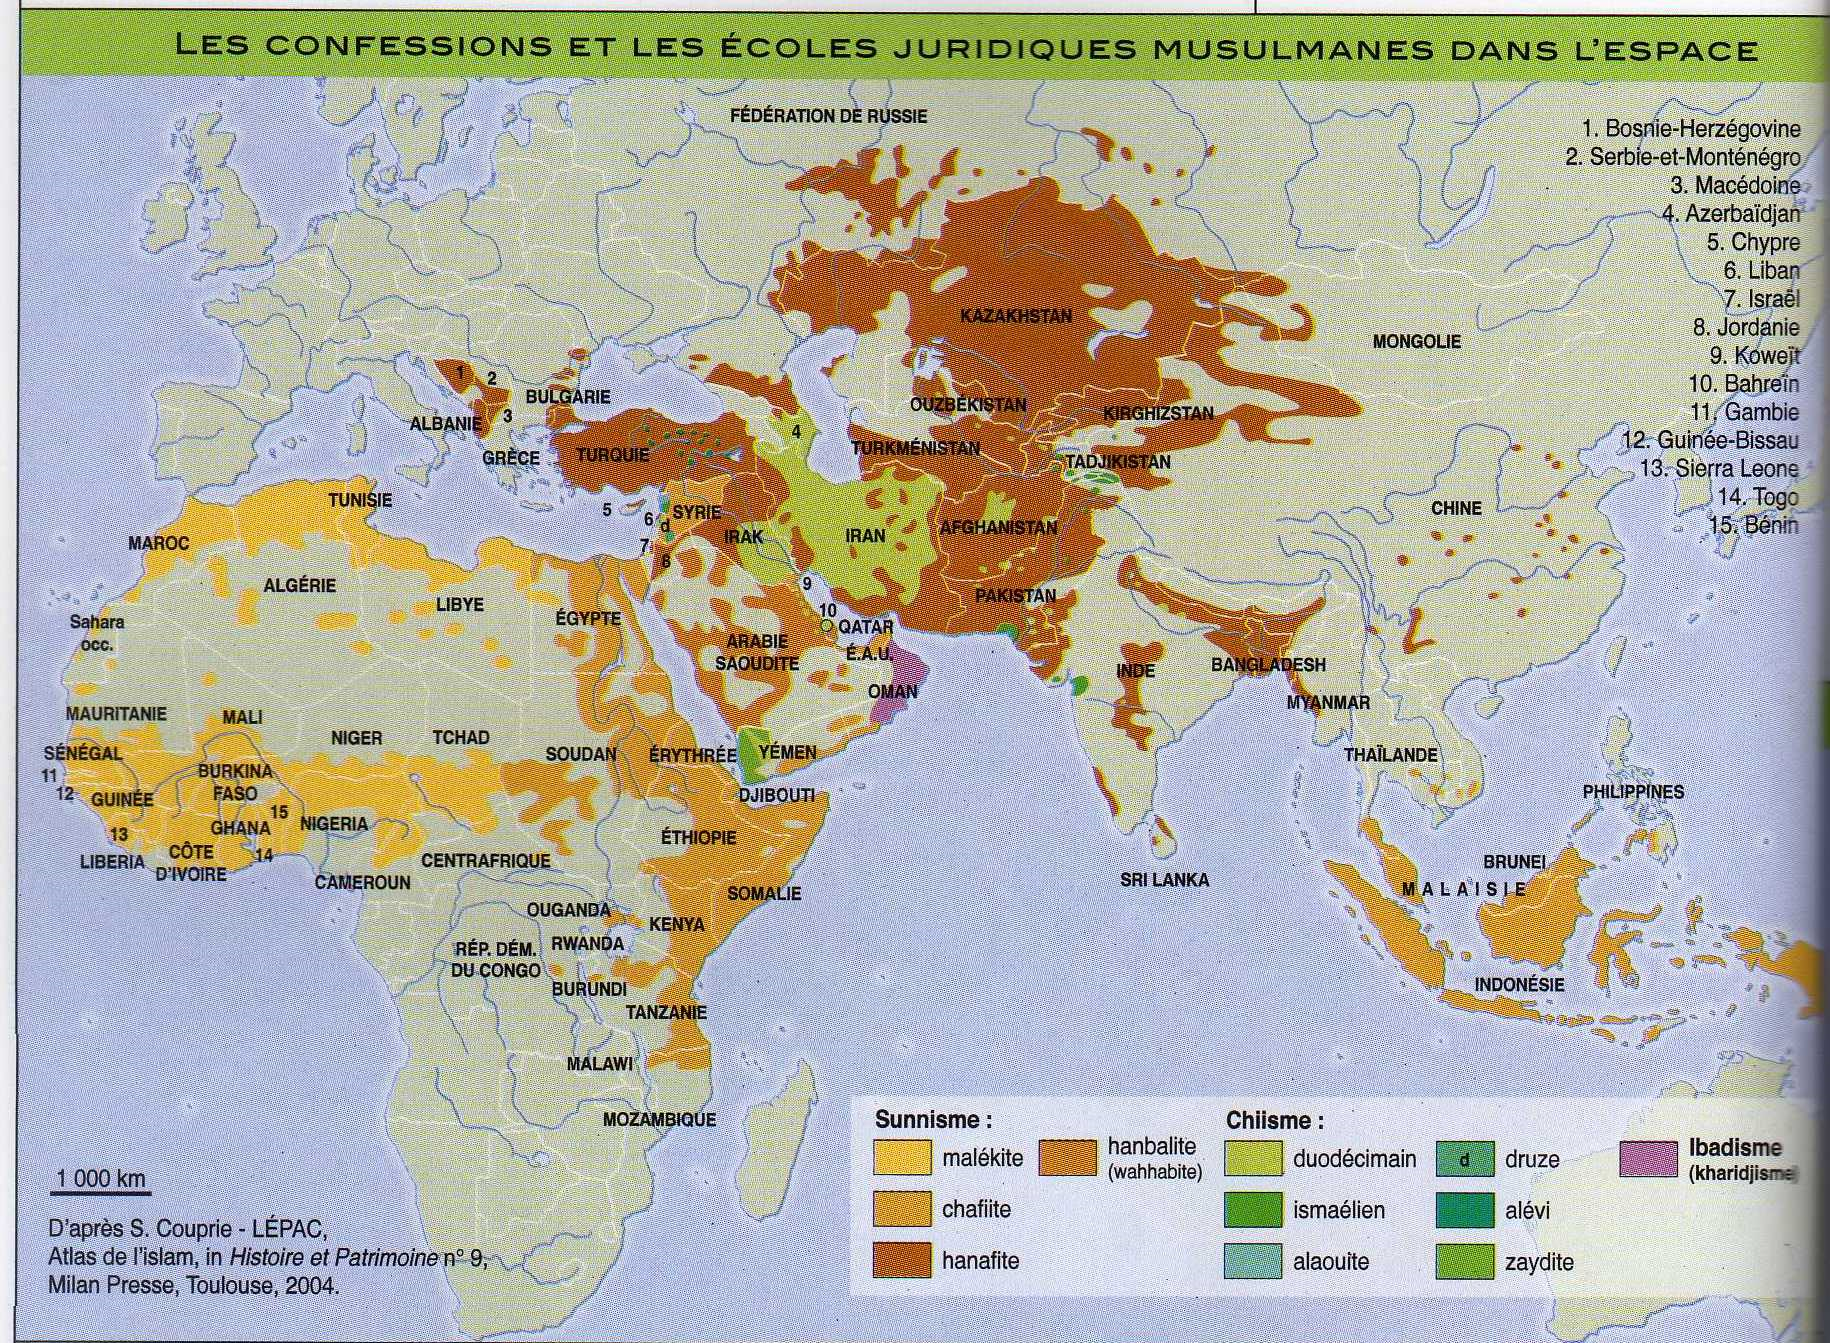
\includegraphics[width=\textwidth]{CourantsIslamContemporain/ImagesCourantsIslamContemporain/CarteSunnisme.png}
 
    \label{fig:my_label}
\end{figure}



\bi 
\item  malékisme : Afrique Nord et ouest.
\item Chafiite : Est de l'Afrique et surtout Egypte 
\item Hanafite : Turquie, asie Centrale, Inde. \textit{les empires turques}
\item Hanbalite : surtout Arabie Saoudite, transformé en \textit{Wahhabisme} au XX, avec une extension au dela de l'Arabie Saoudite en 1960.
\ei 


\subsection{Trois grands courants dans le sh'isme}


\begin{Synthesis}[divergence en Si'isme : les courants]
Des désaccords sur Qui est Imam et sur la \textit{nature de l'Imam}. Il peut être investi de pouvoirs divins.
\end{Synthesis}

\bi 
\item Les duodécimains (ils reconnaissent 12 imams) : les shi'ites Iraniens
\item les Ismaeliens ou septimains (7 imams, l'Aga Khan), Liban.
\item zaydites (5 imams) : Yemen. Au niveau de la doctrine, ils reconnaissent peu de pouvoirs divins aux Imams (proches des Sunnites de ce point de vue).
\ei 
Les Ibadites sont Khajidites. Les druzes et les Alaouites (Alevi en Turc) sont issus du shi'isme (en se proclamant le Maadi) mais ne sont pas considérés comme musulmans par les autres musulmans.  A ne pas confondre à la famille Alaouites au Maroc qui sont tout à fait sunnite (Alaouite veut dire descendant d'Ali). L'Iran reconnait les Alaouites comme shi'ites pour des raisons politiques. 

\subsection{diversité culturelle}
L'islam s'est acculturé aux cultures qu'il a rencontré.
\paragraph{Mosquée}
Le seul élément architectural à une mosquée est la qibla qui indique la Mecque : le Mihrab.

\bi
\item la mosquée bleue a été constituée sur le plan de Sainte Sophie
\item Mosquée de Djenné.
\item La mosquée de Lagos : représente un style baroque brésilien.
\item Xian
\item la grande mosquée de Paris : sur l'image d'une mosquée marocaine
\item Mosquée contemporaine de Créteil

\ei 

\paragraph{L'habit féminin} D'après le Hadith "on ne doit montrer que les mains et le visage". 

\bi
\item les danseuses de cours à Surakarta
\item la burqa, avec grillage sur les yeux, asie centrale et Afghanistan dans certains milieux
\item des vétements de couleur et le shadri, vêtement traditionnel en Asie centrale paysanne voile que l'on met différemment selon qu'on est seul, ...
\item en Afrique, habit d'abord ethnique et non religieux. 
\item En France, les jeunes : le bandeau pour tenir le foulard et le foulard coloré. et certaines ne portent pas le foulard
\ei 

\paragraph{Pourquoi une impression d'uniformisation} La mondialisation crée l'uniformisation et certains courants wahhabites incitent à l'uniformisation sur l'influence saoudite.

\subsection{Observer l'islam}

 
\newlength\q
\setlength\q{\dimexpr .5\textwidth -2\tabcolsep}

\begin{table}[h!]
\sidecaption{\textit{Observer l'Islam} Clifford Geerzt, il a été au Maroc et en Indonésie}
%\begin{tabular}{p[7cm]p[7cm]}
\noindent\begin{tabular}{p{\q}p{\q}}
\toprule
\textbf{Maroc}                                                     & \textbf{Indonésie}                                               \\ 
\midrule
Tribale                                                            & Paysanne                                                         \\
\textit{Audace}                                                    & \textit{Application}                                             \\
une culture préalable moins riche                                  & L'islam est arrivé sur une civilisation hindouiste et bouddhiste \\
Un islam de dévotion aux saints (en particulier le saint guerrier) , austérité morale, pouvoirs magiques, piété agressive & malléable, syncrétique  \\
Uniformisation, facteur de civilisation & diversification, multiforme\\

\bottomrule
\end{tabular}
\end{table}

\subsection{Bibliographie}

\begin{quote}
\textbf{Atlas}

*DUPONT, Anne-Laure \emph{Atlas de l'islam dans le monde}, nouv. éd.,
Autrement, Paris, 2014. GUIDERE, Mathieu \emph{Atlas des pays arabes. De
la révolution aux démocraties}, Autrement, Paris,

2012.
\end{quote}

\hypertarget{ouvrages}{%
\subsection{Ouvrages}\label{ouvrages}}

\begin{quote}
BURESI, Pascal \emph{Géo-histoire de l'islam}, Belin, Paris, 2005.

GEERTZ, Clifford \emph{Observer l'islam : changements religieux au Maroc
et en Indonésie}, La Découverte, Paris, 1992.

*MERVIN, Sabrina \emph{Histoire de l'Islam. Doctrines et Fondements},
nouv. éd., Flammarion, 2016.

DE PLANHOL, Xavier \emph{Les nations du prophète}, \emph{manuel
géographique de politique musulmane}, Fayard, Paris, 1993.
\end{quote}
\chapter{Les racines de la réforme : le
renouveau islamique des XVIIe-XVIIIe
siècles}
\mn{(24/01/2022)}

Un leçon sur les racines de cette diversité, et de tous ces courants au sein du monde Sunnisme. Tout cela part du désir de "\textit{Réforme}" qui part à un retour au source. Et cela peut donner des solutions très diverses, soit des lectures libérales ou des lectures fondamentalistes (un peu comme les évangéliques protestants).
Plutôt \textit{Renouveau} que \textit{Réforme}.

%------------------------------------------------
\section{La crise interne du monde musulman}
\subsection{Déclin des grands empires}

 
 \begin{Synthesis}[Date Symbolique]
 1798 : Napoléon en Egypte, date symbolique de la rencontre du monde musulman avec la modernité occidentale.
 \end{Synthesis}
 Cette lecture n'est pas fausse et va donner lieu au \textit{réformisme} mais c'est une lecture occidentalo-centrée.
 En réalité, cela a commencé plus tôt. Un désir né courant XVII et interne au monde musulman.
 
Les trois grands empires musulmans de l'époque rentrent en crise : 

\begin{table}[h!]
    \sidecaption{Les trois grands Empires musulmans}


%\newlength\q
\setlength\q{\dimexpr .25\textwidth -2\tabcolsep}
\footnotesize%
\noindent\begin{tabular}{p{\q}p{\q}p{\q}p{\q}}
\toprule
                & Fondation           & Apogée                            & Fin                                                                                \\
\midrule
Empire Safavide & 1501 (Ismaïl   1er) & Abbas Ier (1588-1629)             & 1736                                                                               \\
Empire Moghol   & 1526 (Babur)        & Akbar (1556-1605)                 &  1857 (existence symbolique après 1761)  \\
Empire Ottoman  & 1299 (Osman 1er)    & Soliman le Magnifique (1520-1566) & 1922                                        \\
\bottomrule
\end{tabular}


    \label{tab:my_label}
\end{table}
 
 
 
 \paragraph{Raisons économiques} Les portugais contournent l'Afrique et contournent les empires musulmans.  
 \paragraph{crises politiques} au sein de ces empires, trop grands. 
 \paragraph{Des voisins puissants} Ces Etats vont perdre des territoires face à des puissances qui ne sont pas musulmanes. L'empire Safavide est attaqué par les Ousbeks. L'Empire Moghol en XVIII siècle s'effondre devant l'empire Marathe (Hindou). L'empire Ottoman resiste mais décline depuis 1686 (siège de Vienne). 
 \begin{itemize}
     \item  {Affaiblissement des sultanats Indonésiens} face aux Hollandais. Java est annexé en 1800. 
  \item {En Chine} les musulmans Chinois (Hui) subissent des pressions des Manchous.
   \item  {Afrique} Les bambaras conquièrent Djenné, Tombouctou et Gao. Les portugais en Océanie. 
  \item {En Asie Centrale}, avancée des Russes (XIVII : Kazakstan et reste de l'Asie Centrale au XIX).
 \end{itemize}

 \paragraph{A la fin du XVI} 1591 : deuxième millénaire de l'Islam; sentiment millénariste. \mn{Calendrier lunaire, donc décalage}
 
 
 
\subsection{Problèmes doctrinaux et religieux}

\paragraph{Un raidissement des écoles juridiques au XVII}
Elles s'accusent les unes les autres de ne pas être juste, sentiment de division du monde sunnite.

\paragraph{Décadence du monde Soufi} On a tendance à considérer les soufis comme à la marge du monde musulman. Pourtant, elles ont joué un rôle social déterminant voire politique. Or, à l'époque, elles sont en crise.
\begin{itemize}
    \item {En faisant des Etats dans l'Etat} 
\item {Laxisme spirituel} Un soufi n'est plus tenu de suivre les prescriptions de l'Islam.
\item {Un rôle de plus en plus important du Sheykh}, le maitre spirituel de la Confrérie, qui transmet la \emph{Baraka}.
\item {Des pratiques spéctaculaire} Le fakirisme. le \emph{Dhikr}, rappel du nom de Dieu et l'on atteint l'Etat de transe, et vont marcher sur des braises. 

\end{itemize}



%------------------------------------------------
\section{L'aspiration au
  renouveau}
\subsection{Millénarisme}


 \begin{Def}[rapport au temps Involutif]
 L'Islam se tourne vers le passé, en Islam, les prophètes viennent toujours rappelés ce qui a été donné à l'origine. et le problème est que les hommes déforment le message transmis. Donc Dieu envoie de nouveaux prophètes pour restaurer le message originel. \textit{le temps corrompt.}
 
 \end{Def}
 vs Evolutif. 
 
 Ce qui fait que Mohammad est le dernier des prophètes, c'est que le message est transmis intact, pour la première fois, donc plus besoin de nouveaux prophètes. Autant, la \textit{pratique} peut se corrompre. 
 Un hadith dit : 
 \begin{quote}
     Slt un dixième de la pratique suffira pour sauver le monde.
 \end{quote}
 
 \begin{Def}[Moujaddid]
 de la racine JDD, nouveau, celui qui renouvelle l'Islam pour le mettre tel qu'il était à l'origine. 
 \end{Def}

 
 \begin{Def}[tajdid]
 Tajdid, le renouveau, qui doit venir régulièrement. Chaque siècle Dieu envoie un \textit{Moujaddid} selon un Hadith du Prophète.
 \end{Def}
 
 
 Il peut y en avoir plus mais à chaque siècle, il y a un grand moujaddid, savant, qui ne fait pas forcément au sein de la communauté. 
  \begin{Ex}
 Ghazali est considéré comme un Moujaddid
 \end{Ex}
 
 
 \subsection{Quelques grandes figures de la \textit{pre-Reforme}}
 

\paragraph{Ahamad Sirhindi} (Inde, 1564-1624) , essaye de rénover l'Islam et réforme une confrérie, la \emph{Naqshbandiyya} réformée (mujaddidi). 
\paragraph{Muhaddidi} Restaurer le monde musulman et restaurer l'Islam dans sa pureté originelle. Il va opposer 
\begin{itemize}
    \item le \emph{taqlid}, l'imitation (péjorative, servile, non réfléchie) et
    \item l'\emph{ijtihad}, l'effort d'interprétation du Coran et de la Sunna. Retourner aux sources scripturaires pour restrouver le sens authentique de l'Islam
    \item pour éliminer la \emph{bid'a}, très péjoratif, l'innovation
\end{itemize}  

On peut distinguer deux courants : un courant plus libéral et l'un plus fondamentaliste :
\begin{itemize}
    \item le rapport à la Tradition : fondamentaliste ne vont considérer que le Coran et la Sunna, en critiquant les élaborations savantes de l'Islam. 
    \item ce sur quoi va porter l'\emph{ijtihad}, soit limité sur les versets peu clairs du Coran, soit plus large pour le savant et les différentes sciences qui vont être convoquées pour l'ijtihad.
\end{itemize}


\paragraph{Muhammad 'Abd Al-Wahhab } 'Arabie, 1703-1792). Voir p. \pageref{Theol:AlWahhab}

\paragraph{Shah Wali Allah} (Inde, 1703-1762), \label{Theo:waliAllah} a eu les mêmes professeurs que Al-Wahhab ! et l'un des premiers à traduire le Coran dans une langue vernaculaire (en persan). Effort d'acculturation dans le contexte Moghol et Indou. 




 
%------------------------------------------------
\section{Les voies du renouveau} 
\subsection{Les confréries soufies}

La création de néo-confrérie
\begin{itemize}
    \item lutter contre un laxisme moral
    \item lutter contre le pouvoir du Sheykh.
    \item insister sur le côté social, en prenant en charge la société (vs gnosticime ?).
\end{itemize}
\mn{Soufi : \pageref{Def:SoufiNaqchabandiya}, \pageref{Def:Soufiqādirīya} }




\paragraph{Ahmad Al Tijani} (Algérie 1737, 1815). Et fonde la \emph{\textbf{tijaniyya}}, un groupe toujours très présent en Afrique du Nord. Normalement un Sheykh insiste sur la chaine d'initiation qui remonte au prophète. Lui, va être initié directement en rêve par le Prophète.

\paragraph{Abdurrauf al-Singkili} (Aceh, Indonésie, 1615-1693)

\paragraph{Abdelkarim al-Samman} (Soudan, 1718-1776) => sammaniyya

Au sénégal, aussi une confrérie de type réformée. 
\mn{A completer carte Carte moderne. Il y avait 24 confréries soufis en Arabie avant le Wahhabisme}




%---------------------------------------
\subsection{Les centres de pèlerinage : La Mecque et Médine}

La Mecque et Médine jouent un rôle essentiel, du fait du Hajj. Du fait de l'Empire Ottoman, il y a pacification des parcours du pélerinage, par ailleurs incités par l'Empire.
Et par ailleurs, des centres de formation s'implémentent à la Mecque.  On en profite pour étudier. Se croisent des savants de différentes origines.
Non seulement les centres d'étude mais aussi les confréries, avec leur Sheykh les plus importants s'installant à Médine ou la Mecque. Ils sont initiés à l'enseignement Moujaddidi et vont réformer la confrérie à laquelle ils appartiennent, selon un modèle qui se répète.




%------------------------------------------------
\section{Un aspect particulier : les jihads aux marges du monde   musulman} 


\begin{figure}[h!]
    \centering
        \sidecaption{Le « renouveau » des marges du monde musulman (XVIIIe-XIXe
siècle)  \emph{L'atlas de l'islam depuis 1500}, F. Robinson, Nathan, 1987  
Des petits Etats vont se créer sur des bases confrériques et dont la mission de faire le jihad.
}
 \includegraphics[width=\textwidth]{CourantsIslamContemporain/ImagesCourantsIslamContemporain/image1.jpeg}

    \label{fig:le-renouveau-des-marges-du-monde-musulman-xviiie-xixe-siuxe8cle}
\end{figure}


\subsection{Situation particulière des zones marginales}


Pourquoi on les retrouve aux marges du monde musulman ? Il y a un besoin de purification et l'islamisation par rapport à des populations hétérogènes. Mais aussi, parce que ces zones ne sont pas controlées par les grands empires musulmans qui ne tolèrent pas ces confréries.
Le jihad se porte d'abord sur les musulmans eux-mêmes, pour qu'ils deviennent musulmans puis contre les puissances extérieures ou non musulmanes qui controlent ces zones. 

\paragraph{Une structure Etatique} Le Sheykh est le chef, \emph{Commandeur des Croyants} - on fait référence aux premiers temps musulmans, on prête allégeance, et avec une approche puritaine, très forte pratique. \mn{Des analogiques avec DAESH, qui se réfèrent eux aussi aux temps de l'Islam}

\paragraph{Une accélération de l'Islamisation}


\subsection{Quelques exemples}

\paragraph{Spectre Temporel 1680-1920}{1680, Etat de Bondou} Afrique de l'Ouest jusqu'e l'Etat Mahdiste (Somalie) 1899-1920.

\paragraph{Chine - Ma Ming-hsin} Réveil religieux des communautés chinoises sous la pression des Manchous. Ma Ming-hsin (1719-1781) lorsqu'il est à la Mecque, il fonde une confrérie réformée, la \textit{Nouvelle Secte} et entre en opposition contre les autorités locales, qui appelle en soutien la dynastie Manchoue des Ming. Ming-Hsin est décapité. Il y aura d'autres révoltes plus tard, du Kan-Su et du Chen-Si (1862) et du Yunnan (1856)

\paragraph{Indonésie - Jajji Miskin} Le mouvement Padri à Sumatra (1803-1845). Après le Hajj, en 1803, il prend le contrôle de villages et va imposer sa vision de l'Islam, interdit les pratiques populaires et proclament le Jihad contre les autres villages et les pouvoirs. 1820 : les Hollandais reviennent dans la région et on a une transformation de ce mouvement contre un Jihad contre les Hollandais. Eliminé par les Hollandais.

\paragraph{Nigéria - Califat de Sokoto} Uthman da Fodio (1755-1817) issu d'une famille de savants musulmans, l'enseignement lui vient par la fraderyya\sn{revoir} et crée une communauté qui le reconnait comme \textit{commandeur des Croyants}, s'oppose aux pouvoirs locaux et va être défait par la Grande Bretagne.


\begin{Synthesis}
\begin{itemize}
Ce renouveau : 
    \item Avant la rencontre de l'Occident
    \item lié à des thèmes de crises internes
    \item des thématiques que l'on retrouvera : retourne aux sources scripturaires
    \item C'est assez fascinant de voir la circulation des idées, liée autour du \textit{Hajj}
\end{itemize}


\end{Synthesis}

%------------------------------------------------

 



 



\paragraph{Soufis du Badakhshân : un renouveau confrérique entre
l'Inde et l'Asie centrale}
\mn{Alexandre Papas, \emph{Cahiers d'Asie Centrale}, n° 11-12, 2004, p.
87-102 (extraits -- texte expurgé)}
 
 
\subparagraph{Éléments de biographie d'un soufi
badakhshânais} 
\mn{le Badakhshân est entre l'Afghanistan et le Tajikistan}
\begin{quote}
Mawlânâ Mîr Ghiyâs al-Dîn \label{Theo:MawlanaMirGhiyasAlDin} naît en 1117/1705-06 dans la petite localité
de Hisârak, située au cœur du district de la ville de Jirm. Le
grand-père de Mawlânâ a émigré du village de Dahbîd, non loin de
Samarcande, en direction du Badakhshân. La \emph{silsila}\sn{Génération} de la famille
remonte au Prophète et, sur dix générations, au frère d'un grand saint
Kubrawî et découvre une généalogie \textit{soufie}. C'est donc au sein d'une des
grandes familles \emph{muhâjir}\sn{Emigré, en référence aux premiers musulmans qui ont suivi le Prophète à Médine} de l'aristocratie religieuse du
Badakhshân que naît Ghiyâsî.

{[}\ldots{]}

C'est précisément pour l'Inde -- destination qui concurrence la
Transoxiane savante, en particulier Boukhara, surtout depuis le XVIe
siècle -- que part le jeune Ghiyâsî âgé de 14 ans en quête d'initiation \sn{soufi}.
Cet exil de l'adolescent fait l'objet de deux contes hagiographiques :
 

\begin{itemize}
\item
 
  Le futur shaykh de Ghiyâsî, Shâh Walî Allâh, qui a quitté Sirhind pour
  entreprendre un pèlerinage au mausolée de Bahâ' al-Dîn Naqshband\sn{le fondateur de la confrérie réformée Naqshandayyi} non
  loin de Boukhara, stationne au Badakhshân, à Jirm, chez le père même
  de Ghiyâsî. Le shaykh demande alors à ce dernier de lui amener ses
  enfants, mais perçoit par claire-vue qu'on lui dissimule le jeune
  Mawlânâ qui, en état de \emph{majzûb}\sn{Ils peuvent faire des choses indécentes} « ravi en Dieu », suscite la honte de
  sa famille. À sa vue le shaykh indien cite un vers de Ni'mat Allâh
  Walî Kirmânî. Et au jeune Ghiyâsî de prononcer miraculeusement le
  second vers du distique. Walî Allâh annonce alors qu'à son retour de
  Boukhara il prendra le jeune homme comme disciple et l'emmènera en
  Inde.
  
\item
 
  Dès l'âge de 9 ans Mawlânâ refuse les conseils de sa famille et se
  distingue des autres enfants. Plusieurs nuits, au cours de rêves, lui
  apparaît un homme illuminé qui lui enjoint de partir pour l'Inde où
  lui est promise la rencontre d'un grand saint soufi. Malgré le refus
  de ses parents qui souhaitent marier leur fils, Ghiyâsî parvient à
  quitter le Badakhshân quelques années plus tard. Parvenu à Lahore et
  après un nouveau rêve révélateur, il attend de nombreux jours au
  couvent de Khwâja Khwândamîr, un khalîfa de la Naqshbandiyya, jusqu'au
  jour où il rencontre Shâh Walî Allâh.
 
\end{itemize}

 
Restent les faits : après une formation classique en \emph{madrasa} à
Delhi où le novice rencontre ses premiers maîtres, il devient à Lahore
durant douze années le disciple d'un fameux maître Naqshbandî Mujaddidî.
Il interrompt une unique fois son initiation lorsque le shaykh lui
confie la mission de se rendre au Cachemire afin d'aller chercher un
homme qu'on prétend thaumaturge et que Walî Allâh souhaite convertir à
l'islam et initier à sa \emph{tarîqat}\sn{confrérie}. Au terme de ses douze années de
noviciat, le shaykh lui enjoint de retourner à sa terre natale pour
propager la confrérie. De retour au Badakhshân, Ghiyâsî âgé de trente
ans environ et qui a obtenu le rang de \emph{mawlawiyyat}\sn{maître}, fait office
d'enseignant à la \emph{madrasa} Jâmi'-i Islâmî du district de Jirm. Il
est ensuite convié à Fayz Âbâd à la cour de Sultân Shâh, laquelle abrite
des savants et des poètes venus d'Inde et d'Iran, dont certains
acquièrent grande réputation. C'est là que Ghiyâsî compose son œuvre
poétique et mystique. C'est également là, de son \emph{khânaqâh}\sn{couvent soufi, Ḵānqāh ou ḵānāqāh, fut d'abord un lieu destiné à abriter les spécialistes et savants religieux musulmans (‘ulamâ’), une sorte d'équivalent des couvents chrétiens. Ces établissements ont été ensuite réservés aux soufis.}, qu'il
dirige son enseignement, suivis par de nombreux disciples venus de
toutes les régions alentours. Le soufi badakhshânais devient aussi le
directeur spirituel de Sultân Shâh. Et lorsque ce dernier est capturé à
Qunduz par les ouzbeks du Qataghân en 1179/1765, le vieux maître
conseille durant trois ans le fils et suppléant du shah emprisonné, Mîr
Muhammad Shâh. D'un tel succès et d'une telle influence, Ghiyâsî
apparaît comme l'un des principaux promoteurs de la Mujaddidiyya dans le
Nord de l'Afghanistan.

{[}\ldots{]}
\end{quote}

\begin{Prop}
On retrouve des noms : Walî Allâh (cf p. \pageref{Theo:waliAllah}; l'importance du réseau confrérique; et rôle social (il devient le conseil du sultan).
\end{Prop}

\subparagraph{Savants et soufis au croisement du
Badakhshân}
Le Pamir est un sanctuaire pour les savants hétérodoxes ou bannis (cf Unwân banni d'Egypte du fait de sa lutte sociale).

\begin{quote}
Malgré les obstacles géographiques et en dépit des troubles politiques
qui affectent la fin du XVIII\textsuperscript{e} siècle, le Badakhshân
reçoit la visite de savants religieux qui, pour certains, décident de
s'y installer et interrompent définitivement leur voyage vers l'Inde ou
vers la Transoxiane. Il faut rappeler ici que le Pamir a, de façon
continue dans l'histoire, servi de sanctuaire à des individus frappés
d'ostracisme ou fuyant la répression dans leur région natale. Mais au cours du
XVIII\textsuperscript{e} siècle le sanctuaire se mue en lieu de
renaissance où fleurissent \emph{madrasa}\sn{lieu d'enseignement religieux} et couvent soufis. Le
\emph{Armaghân-i Badakhshân} mentionne le cas de deux étudiants de
Peshawar, Mîr Ahmad Mujaddidî dit `Izhâr' (m. 1259/1843) et son frère
Muhammad Anwar qui, à une date indéterminée durant le règne de Mîr
Muhammad Shâh, se rendent d'abord à Boukhara afin d'obtenir les
compétences du rang de \emph{`âlim}\sn{savant} et qui, lors de leur retour,
s'installent et officient au Badakhshân, pour le premier à Jirm, pour le
second à Bahârak.

Un autre cas de figure est celui, analogue à Ghiyâsî, de ces
badakhshânais qui partent se former aux sciences religieuses, et
éventuellement au soufisme, dans les grands centres de savoir du monde
musulman, proches ou lointains. De ce point de vue, le cas le plus
intéressant -- et malheureusement le plus douloureux faute
d'informations suffisantes et dans l'absence de vestiges de son œuvre --
est celui de Sayyid Abâ al-Hasan « `Unwân ». Né à Jirm en 1123/1711, il
quitte le Badakhshân pour Boukhara afin d'acquérir une formation
théologique. De là `Unwân se rend au pèlerinage de La Mecque et à
Médine, puis il s'installe durant 18 ans en Egypte, probablement au
Caire, où il poursuit son acquisition des sciences islamiques classiques
et commence à enseigner. Mais `Unwân ne se contente pas de dispenser un
enseignement religieux, il prend parti pour les classes populaires
égyptiennes et contre leur oppression par les propriétaires terriens.
C'est du moins la réputation qu'il gagne selon le \emph{Armaghân-i
Badakhshân}, et qui lui vaut d'être banni d'Egypte. `Unwân part alors
pour Istanbul, rejoint Boukhara et reprend son enseignement. `Unwân, qui
prône l'unité de la Communauté des Croyants (\emph{umma}), décide
d'aller prêcher la concorde (\emph{âshtî}) dans le Caucase, peut-être au
moment de l'activisme Naqshbandî de Shaykh Mansûr dans les années 1780.
Mais il renonce à son projet et entre dans une retraite spirituelle
jusqu'à sa mort en 1206/1791, sans être retourné au Badakhshân.
{[}\ldots{]}

\end{quote}

\begin{Prop}
 Dans le deuxième paragraphe, `Unwân se forme à la Mecque et Médine (rôle du pélerinage), rôle social en Egypte et pas seulement religieux. L'importance aussi de l'Unité, l'\textit{Umma}. 
\end{Prop}
 
\subsection{Liste des neo confréries}

\paragraph{Naqshbandiyya}: La Mecque, Damas, Yémen, Inde, Asie Centrale \label{Def:Naqshbandiyya}
                     => Caucase, Chine Occidentale + Orientale, Sumatra.

\paragraph{Qadiriyya}: Proche Orient, Irak, Inde, Asie centrale 
                    => Indonésie (Java, Aceh), Caucase, Afrique

\paragraph{Khalwatiyya}: Egypte => nombreuses branches en Afrique :

\begin{itemize}
    \item \textit{Tijaniya}: Algérie => Afrique de l’Ouest
    \item \textit{Sammaniyya}: Soudan
    \item \textit{Idrisiyya}: Maroc => Sanusiyya (Lybie), Sahiliyya (Somalie),
    \item \textit{Murghaniyya} (Erythrée)
\end{itemize}- 
 
%-----------------------------------------------
\subsection{bibliographie}

\begin{quote}


AZRA, Azyumardi \emph{The Origins of Islamic Reformism in Southeast
Asia}, Asian Studies Association of Australia/KITLV Press, Leiden, 2004.

PAPAS, Alexandre \emph{Soufisme et politique entre Chine, Tibet et
Turkestan}, J. Maisonneuve, Paris, 2005.

*ROBINSON, Francis \emph{Atlas de l'Islam depuis 1500}, Nathan, Paris,
1987 (dispo à la FELS)

*VOLL, John R. « Foundation for renewal and reform », in John L.
Esposito ed., \emph{Oxford History of Islam}, Oxford University Press,
1999, pp. 509-547.
\end{quote}
\chapter{Un fruit du « pré-réformisme » : le wahhabisme}
\mn{ \emph{(31/01/2022)}}



 
  \subsection{Muhammad Ibn al Wahhab
  (1702-1792)} 
  \label{Theol:AlWahhab}
    Formation et premières prédications
 
    L'alliance avec Ibn Se`ud
    
 
  \subsection{La doctrine wahhabite} 

 
  Nécessité du retour aux sources
 
  Une notion centrale : le \emph{tawhid} (unicité divine)
  
  La question du \emph{jihad}
 
 
  \subsection{Le devenir du wahhabisme} 
 
    Le wahhabisme et l'Etat saoudien
  
    Une étude de cas : le wahhabisme en Afrique de l'Ouest
    

 
\subsection{ {Glossaire}} 


\paragraph{Personnes} `Abd al --`Aziz Abu Bakr

al-Majmu`i al-Sindi

Ibn Taymiyya Muhammad Ibn Se`ud

\paragraph{Lieux}

al-Azhar al-Dir'iyah

al-Uyaynah (Najd). Basra

Hijaz Huraymila Jeddah Najd

\paragraph{Notions}

ashraf : \emph{descendants du Prophète}

da`wa \emph{: prédication}

fiqh : \emph{droit musulman}

hadith \emph{: fait ou dire du Prophète}

hijra : \emph{« exode »}

ijma\emph{` : consensus des ulamas}

ijtihad : \emph{effort d'interprétation}

kufr \emph{: incroyance /} 

kafir \emph{: infidèle, mécréant}

qiyas \emph{: raisonnement par analogie}

salat : \emph{prière rituelle} 

shirk : \emph{associationnisme} 

taqlid
\emph{: imitation (servile)} 

tawhid : \emph{unicité divine}

zakat :
\emph{aumône légale}


 
\subsection{Les trois Etats Saoudiens} 

 
  {\paragraph{1744 -1818}: une première expansion}
 
 
\emph{1744} alliance Ibn Se`ud /Ibn al-Wahhab
 
\emph{1786} conquête du Najd (`Abd-al-`Aziz)
 
\emph{1792} mort d'Ibn al-Wahhab
 
\emph{1806} conquête de La Mecque
 
\emph{1818} défaite devant les Ottomans
 

 
  {\paragraph{1821-1883}: petit Etat centré sur Riyad (Najd)}
 
  {\paragraph{1901- 2011} : le Royaume d'Arabie Saoudite}
 
 
\emph{1924} conquête de La Mecque. Abdelaziz Ibn Se`ud prend le titre de
roi.

\emph{1939} début de la production pétrolière \emph{1962} création de la
Ligue islamique \emph{1990} début de la guerre du Golfe.
 

 
\subsection{L'Arabie Saoudite et l'économie
pétrolière} 
 
\paragraph{ {Début de la
production}} 

\begin{quote}
1935: premier forage

1939: premier baril de pétrole

⇒ Cartel américain: l'ARAMCO
\end{quote}

 
\paragraph{{Nationalisation de la
production}}


1973: l'Etat s'approprie 25 \% des droits de l'ARAMCO (1974 : 60\%, 1980 : 100\%)


⇒ Saoudi ARAMCO: 95 \% de la production du pays.

 
\paragraph{Evolution du cours du
pétrole} 

\begin{quote}
1973: premier choc pétrolier (guerre de Kippour) =\textgreater{} de 4 à
15 \$/B

1981-1983: deuxième choc pétrolier (Révolution iranienne + guerre
Iran-Irak) =\textgreater{} 36 \$/B 2006-2008: troisième choc pétrolier
(guerre en Irak) =\textgreater142 \$/baril
\end{quote}

\paragraph{{Rente}}: 1973-2002 =\textgreater{} 200 000 milliards
de dollars au total

 %-----------------------------------------------------
\subsection{Extraits du \emph{Kitab at-tawid} (Livre de
l'unicité divine) de Muhammad Ibn Wahhab}
\mn{Traduction et édition établies en Arabie Saoudite}
\paragraph{{Chapitre 1} : \emph{Tawhid}}

\begin{quote}
\emph{Allah-ta`ala} a dit : « Je n'ai créé les djinns et les hommes que
pour qu'ils M'adorent (1 :56)\ldots Et très certainement nous avons
suscité dans chaque communauté un message pour leur dire d'adorer Dieu
et d'écarter le Rebelle (16 :36)\ldots Et voilà que ton Seigneur a
décrété que tu dois n'adorer que Lui et faire preuve de bonté envers tes
parents (17 :23)\ldots Adorez Dieu et ne lui donnez quelque associé que
ce soit (4 :36)\ldots Venez, je vais vous réciter ce que votre Seigneur
vous a interdit ; - ceci : Ne lui associez quoi que ce soit\ldots(6
:151-153) ». Ibn Mas`ud a dit : « Quiconque se propose de vérifier le
testament du Prophète Muhammad (SWA) -- un testament sur lequel le
Prophète a apposé son sceau, qu'il lise ces mots d'Allah : « Venez, je
vais vous réciter ce que votre Seigneur vous a interdit ; - ceci : Ne
lui associez quoi que ce soit\ldots Voilà ce qu'il enjoint » (6 :
151-153)

Mu`adh Ibn Jabal raconta : « Je montai derrière le Prophète (SAW) quand
il me dit : « Ô Mu`adh ! Sais-tu ce que les créatures d'Allah Lui
doivent et ce qui leur est dû ? » Je répondis : « Allah et son Prophète
savent mieux ». Il continua : « Ce que les créatures d'Allah Lui
doivent, c'est de ne jamais associer qui que ce soit avec Lui. Ce qui
leur est dû, c'est qu'il ne punira aucune personne qui ne Lui associe
pas un autre ». Je dis :

« Ô Prophète d'Allah, est-ce que je peux annoncer la bonne nouvelle aux
gens ? » Il répliqua : «Non ! Ne leur dis rien de peur qu'ils comptent
sur la promesse et manquent à leurs devoirs envers Lui». Ce hadith est
mentionné dans deux \emph{Sahihs}.
\end{quote}
D'autres points :


\begin{enumerate}

\item
  \begin{quote}
  La sagesse dans la création du djinn et de l'humanité.
  \end{quote}
\item
  \begin{quote}
  Le service à Allah consiste en le \emph{tawhid}. Car, à l'opposé du
  \emph{tawhid} se trouve l'aliénation d'Allah. (\ldots)
  \end{quote}
\item
  \begin{quote}
  La sagesse d'envoyer des prophètes. (\ldots)
  \end{quote}
\end{enumerate}
\paragraph{{Chapitre 2} : Les vertus du \emph{tawhid} et les
nombreux péchés qu'il expie}
\begin{quote}


\emph{Allah-ta`ala} dit : « Ceux qui ont cru et n'ont point revêtu de
prévarication leur foi\ldots{} » (6 : 82).

(\ldots) Abu Sa`id al Khudriyy rapporta que le Prophète d'Allah (SWA) a
dit : « Quand Musa {[}Moïse{]} demanda à Allah de lui enseigner une
prière qu'il puisse réciter à chaque fois qu'il pensait à Lui ou qu'il
L'évoquait, Allah répondit : « Dis, ô Musa, qu'il n'y a d'autre Dieu
qu'Allah. Musa dit : « Ô Seigneur, tous tes serviteurs prononcent ces
mots ». Allah dit : « Ô Musa, si les sept cieux et tout ce qu'ils
renferment, et les sept terres aussi, si tout cela était pesé contre
cette phrase : « Il n'y a d'autre Dieu qu'Allah », cette dernière
pèserait plus lourd ». Ibn Hibban rapporta cela également et al-Hakim
compléta sa version. Al-Tirmidhi enregistra, avec peu de rédaction, le
récit de Anas à l'effet qu'il entendit le Prophète d'Allah (SWA) dire :
« Allah dit : « Ô Homme ! Si tu venais à Moi avec tous les sacs du monde
remplis de tes péchés, mais avec le témoignage que tu n'associes rien à
Moi, Je viendrais à toi avec tous mes sacs remplis de miséricorde et de
pardon ! ».

    
\end{quote}
\paragraph{{Chapitre 4} : La crainte du \emph{shirk}}
\begin{quote}
Allah -- qu'Il soit loué et glorifié -- dit : « Non, Dieu ne pardonne
pas qu'on Lui donne quelque associé. En deçà, Il pardonne à qui il veut
» (4 : 48, 116)

(\ldots) Dans le hadith, nous lisons : « Ce que je crains le plus pour
vous, c'est le moindre \emph{shirk}. Quand on lui demanda ce que
c'était, le Prophète répondit : « l'hypocrisie ». Dans le Sahih
d'al-Bukhari, nous lisons que Ibn Mas`ud reporta : « Le Prophète d'Allah
(SWA) a dit : « Celui qui rencontre Allah le jour du Jugement sans Lui
avoir associé qui que ce soit ira au Paradis, et celui qui le rencontre
ayant fait le contraire sera consigné en Enfer ».
\end{quote}
\paragraph{{Chapitre 5} : L'appel à témoigner qu'il n'y a d'autre
Dieu qu'Allah}
\begin{quote}
\emph{Allah-ta`ala} a dit : « Dis (ô Muhammad) : `\,`Voici mon sentier,
j'appelle à Dieu'\,' » (12 :108)

Ibn `Abbas (RA) rapporta : « Quand le Prophète d'Allah (SAW) envoya
Mu'adh à al-Yaman, il lui recommanda : `\,`Quand tu rencontres des gens
du Livre, que ta première action soit de leur demander de témoigner
qu'il n'y a d'autre Dieu qu'Allah'\,' ». Selon un autre récit, «
\ldots{} de leur demander de réaliser l'unicité d'Allah. S'ils
t'obéissent, informe-les qu'Allah leur a imposé la \emph{salat} cinq
fois par jour. S'ils t'obéissent en cela, alors informe-les qu'Allah
leur a imposé le devoir de charité qui doit être perçue des riches pour
être distribué aux pauvres. S'ils t'obéissent en cela, ne touche pas à
leurs autres biens et occupe-toi de la plainte de

l'opprimé, car il n'y a aucun obstacle dans son accès à Allah ».
(Rapporté dans les \emph{Sahihs} d'al-Bukhari et de Muslim). (\ldots)
\end{quote}
\paragraph{{Chapitre 17} : L'intercession}
\begin{quote}
Allah -- qu'il soit loué et glorifié -- a dit : « Et par ceci (le
Qur'an), avertis ceux qui, n'ayant pour eux hors de Dieu, ni ami ni
intercesseur, craignent d'être rassemblés vers le Seigneur\ldots{} » (6
: 51). Dis : « A Dieu l'intercession tout entière\ldots{} » (39 : 44).
Qui peut intercéder auprès de Lui que par sa permission ?... (2 : 255).
Et combien d'anges dans les cieux ? Leur intercession ne met au large en
rien, sauf après que Dieu l'a permis, en faveur de qui il veut et qu'il
agrée » (53 : 26). (\ldots)

(\ldots) En tant que catégorie générale du Jour du Jugement en laquelle
les mécréants croient, l'intercession est rejetée par le Qur'an. Le
Prophète (SAW) nous informa qu'en ce jour « il sera amené devant Allah.
Il se prosternera lui-même et louera Allah, plutôt que de demander à
intercéder. Alors on lui dira : « Lève-toi ! Parle maintenant et tu
seras entendu ! Demande et il te sera donné ! Intercède et il te sera
accordé ! » (\ldots) L'intercession est donc là pour les croyants
sincères et candides. Elle n'est accordée que par la permission d'Allah
et n'appartient pas aux associationistes. (\ldots)
\end{quote}
\paragraph{{Chapitre 20} : Condamnation de celui qui invoque Dieu
auprès de la tombe du juste et, a fortiori, de celui qui invoque ce
dernier.}
\begin{quote}
Dans le \emph{Sahih}, A'ishah (RAA) rapporta : « Umm Salmah raconta au
Prophète d'Allah (SAW) qu'elle avait vue une église remplie d'images et
de statues en Abyssinie. Le Prophète dit : « Ceux-là sont les pires de
tous les hommes : lorsqu'un membre juste et vertueux de leur groupe
meurt, ils bâtissent une église sur sa tombe et y installent toutes
sortes d'images pour lui. Ils sont coupables de deux méfaits : celui
d'invoquer quelqu'un auprès d'une tombe et celui d'installer des images
». (\ldots)

Ainsi le Prophète interdit cette pratique et condamna celui qui la
suivait. Faire le \emph{salat} sur une tombe est également interdit,
même si aucune mosquée n'a été construite sur l'emplacement. Telle est
la signification de la déclaration suivante : « On craignait qu'elle ne
soit prise pour une mosquée ». Les Compagnons n'étaient pas supposés
construire une mosquée autour de la tombe du Prophète. Tout endroit
destiné au \emph{salat} ou tout endroit où le \emph{salat} est accompli,
est une mosquée. Tel l'a déclaré le Prophète (SAW) : « Toute la terre
est pour moi une mosquée, un endroit pur (pour accomplir le
\emph{salat}) ».
\end{quote}
\paragraph{{Chapitre 27} : Les motivations mondaines sont des
exemples de \emph{shirk}}
\begin{quote}
\emph{Allah ta'ala} a dit : « Qui aspire à la vie d'ici-bas et à ses
parures, nous leur solderons ce qu'ils y auront fait : ils ne subiront
pas de perte ! Voilà ceux qui, dans la vie dernière, n'ont pour partage
que le Feu : leurs réalisations d'ici-bas ont crevé ! Nulles sont leurs
œuvres ! (11 : 15-16).

Abu Hurayrah (RAA) rapporta ce hadith \emph{sahih} suivant : « Le
prophète d'Allah (SAW) a dit : `\,`Malheur à l'esclave du dinar !
Malheur à l'esclave du dirham ! Malheur à l'esclave du khamilah !
(\ldots)
\end{quote}
\paragraph{{Chapitre 38} : Obéir aux ulamas ou aux gouvernants
qui légitiment ce qui est interdit ou interdisent ce qui est légitime,
c'est les associer à Allah.}
\begin{quote}
Ibn `Abbas a dit : « Je vous dis que `\,`le Prophète d'Allah (SAW) a dit
ceci et vous dites que `Abu Bakr et `Umar ont dit quelque chose d'autre
?'\,' Le ciel va bientôt vous cracher des pierres sur la tête !! »

Ahmad ibn Hanbal a dit : « Très étranges, en effet, sont ceux qui,
sachant le véritable \emph{isnad} (d'un commandement du Prophète), se
tiennent quand même à l'opinion de Sufyan. Allah lui-même a dit : « Que
ceux donc qui s'opposent à son commandement prennent garde qu'une
tentation ne les atteigne, ou que ne les atteigne un châtiment
douloureux ». (24 : 63). Savez-vous ce que peut être une telle tentation
? C'est le \emph{shirk}. Car, désobéir au Prophète dans certains de ses
commandements, c'est pratiquement comme si on reniait son message et on
s'attirait le Feu.

\end{quote}


\section{bibliographie}

 

\begin{itemize}
\item
 
  IBN AL-WAHHAB, Muhammad \emph{L'unicité de Dieu}, al Qalam, Paris,
  2001.
 


 \item
MENORET, Pascal \emph{L'Énigme saoudienne. Les Saoudiens et le monde
1744-2003}, La Découverte, Paris, 2003.
\item
MIRAN, Marie ; RIALLAND, Maëlle « Dossier Wahhabisme », \emph{Islam et
sociétés au Sud du Sahara}, n°12, 1998, Paris.
\item
MOULINE, Nabil \emph{Les Clercs de l'islam. Autorité religieuse et
pouvoir politique en Arabie Saoudite
(XVIII\textsuperscript{e}-XXI\textsuperscript{e} siècles)}, Paris, PUF,
2011.
\item
  \emph{Histoire de l'Arabie
saoudite}, Paris, Flammarion, 2013.
\item
REDISSI Hamadi \emph{Une histoire du wahhabisme. Comment l'islam
sectaire est devenu l'islam}, Paris, Seuil, 2016.
 \end{itemize}
\chapter{Le mouvement réformiste (fin XIXe - début XXe)}
  \mn{(07/02/2022)}
 
 
  
  `ABDUH Muhammad, \emph{Rissalat ai Tawhid - Exposé de la religion
  musulmane}, Geuthner, Paris, 1925, trad. fr. et introduction B. Michel
  et Ch. Moustapha Abdel Razik.
  
 
  
  AL-AFGHANI Jamâl ad-Din, \emph{La réfutation des matérialistes},
  Geuthner, Paris, 1942, trad. fr. A.-M. Goichon. Textes divers in:
  \emph{Orient}, 1962, N° 21 p. 89-115, N°22 p. 125-160, N° 23 p. 169-
  198, N' 24 p. 125-152 et \emph{Orient}, 1963, N° 25 p. 141-152.
 


HADDAD, Mohammed \emph{Le réformisme musulman : une histoire critique},
Paris, Mimesis, 2013. HOURANI, Albert \emph{La pensée arabe et
l'Occident,} Groupe Naufal Europe, Paris, 1991.

JOMIER Jacques \emph{Le Commentaire coranique du Manâr}, Maisonneuve,
Paris, 1954.

MERAD Ali \emph{Le réformisme musulman en Algérie de 1925 à 1940. Essai
d'histoire religieuse et sociale}, Paris, Mouton et Cie, 1967.
 \emph{Ibn Bâdis,
commentateur du Coran}, Geuthner, Paris, 1971.

METCALF, Barbara \emph{Islamic Revival in British India 1860-1900},
Princeton University Press, 1982.

TROLL, Christian \emph{Sayyid Ahmad Khân. A Reinterpretation of Muslim
Theology}, Vikas Publ.

House, New Delhi, 1978.



 \section{Introduction : Arrière fond positiviste}
 
 \paragraph{Auguste Comte}
 
 \paragraph{idée de progrès} Évolutionnisme de société. Le progrès est porté par l'occident. Vision des sociétés évoluant vers un mieux, du coup, hiérarchisation des sociétés, entre les sociétés archaïques et celles qui s'appuient sur la Raison et ont dépassé le stade de la religion.
 
 \paragraph{Acceptation des valeurs occidentales} souveraineté du peuple; droits individuels; liberté d'expression. 
 
 \paragraph{Un discours critique de la Religion} 
 
  %-----------------------------------------------------------------------------------
  \section{Les « Occidentalisants »}
  
\paragraph{trois premiers quarts du XIX} jeunes de l'élite de l'empire Ottoman. L'empire cherche à se réformer en introduisant des éléments européeans. L'Empire Ottoman envoie des jeunes en France pour se former.

\paragraph{Tahtawi} Egyptien, a vécu 5 ans en France (1826-1831). A été ensuite dans l'administration ottomane. \textit{L'Or de Paris}\sn{très intéressant à lire}

\paragraph{Khayr ad-din} Caucasien, installé en Tunisie. A vécu à Paris (1852-1856).

\paragraph{Jeunes ottomans} dans le contexte turque. 

\paragraph{Ils notent le désir de progrès} A la différence de Al Wahhab qui est soupçonneux de l'\textit{innovation}, on valorise le changement social : 
\begin{quote}
    quiconque maitrise un art désire inventer quelque chose inconnu auparavant \sn{Or de Paris}
\end{quote}

 
 \paragraph{État}  Sur le plan politique, une compréhension différente de l'État. Dans le cadre classique, l'État doit assurer la justice. Or, ici l'État encadre le progrès de la société. Ils sont convaincus que ce sont les institutions politiques qui sont à l'origine de la force des États occidentaux. Par contre, ils vont être en retrait sur l'approche critique de la religion du positivisme.
 
 \paragraph{les lumières ont émancipé l'Europe de l'obscurantisme chrétien} avec une pointe polémique : les lumières viennent de la philosophie musulmane, et donc adopter les lumières pour les musulmans, ce n'est pas trahir le patrimoine musulman, c'est se le réapproprier. \sn{C'est la pointe de Tariq Ramadan dans les années 1990}.
 
 \paragraph{Principes politiques} Ils vont associer les principes démocratiques au principe de la \emph{Shura}, \textit{consultation}, principe coranique de consultation des notables, reinterprété dans un contexte moderne.
 \begin{Def}[shura]
    \emph{ intention} - consultation
\end{Def} 
 \paragraph{droit musulman} dans un cadre musulman, Il faut moderniser le droit musulman pour qu'il puisse accompagner le développement de la société. Ils pronent une unification du droit, une seule école, moderne et uniforme. Il faut viser à l'éducation des jurisconsultes, dans un cadre moderne. 
  
  %-----------------------------------------------------------------------------------
  \section{Trois grands réformistes}
   
   Après les occidentalisants, qui préfigurent les modernistes, il y a les réformistes que l'on verra à travers trois figures.
   
   \paragraph{Seyyed Ahmad Khan (1817-1898)} Il ne sort pas de nul part, son père est soufi et sa mère a été formé dans une école fondé par Walî Allâh (P \pageref{Theo:waliAllah}). Très grande figure en Inde
   
   \paragraph{Jamal ad-din Al Afghani (1839-1897)} formé en Inde mais action dans l'Empire Ottoman (séjour important en Egypte (1871-79)) et un autre à Paris où il est exilé (1881-1883). C'est un activiste  : revues, société secrète. Son but est de lutter contre la colonisation. Il finit sa vie sous surveillance ottomane.
   
    \paragraph{Muhammad Abduh} Egyptien, successeur d'Al Afghani. Il a ensuite développé sa propre pensée. Surtout en Egypte mais a partagé le séjour parisien de \textit{Aghani} puis au Liban. On lui a interdit d'enseigner mais il a été nommé grand mufti d'Egypte (1899). On avait moins peur de son activité du droit que de son activité sur les jeunes en tant qu'enseignant. Fonde aussi une école qui va évoluer différemment. 
    
    \paragraph{Avancée coloniale plus avancée} La colonisation s'est accentuée : les occidentaux apparaissent comme une menace politique. Peur du colonialisme. Le positivisme s'est aussi accentué. Ils doivent se situer dans le rapport entre Foi et Raison. 
   
   \paragraph{Héritiers du pre-réformisme} En inde en particulier, décadence du monde musulman. beaucoup plus faibles que l'occident, parce que \textit{nous avons perdu l'authenticité de la Foi musulmane}. Pour retrouver notre puissance, il faut retrouver l'authenticité de la pratique et la Foi musulmane.
   
   \paragraph{Mais des différences} Mais la différence avec la pré-reforme, cela passe par la pensée des lumières qu'ils accueillent de façon positive. Importance de la \textit{raison}. Par ailleurs, à la suite de \textit{Guizot}\sn{François Guizot, \textit{Histoire de la Civilisation en Europe}}, il pense l'Islam comme civilisation et pas uniquement comme Religion. Qui dit civilisation implique Progrès. 
   
  
  %----------------------------------------------------------------------------------- 
  \section{Foi et raison}
  
 \paragraph{Renan } Dans un discours retentissant à la Sorobonne, il affirme que les races sémites sont opposés à la Religion.
 
 \paragraph{Réponse d'Afghani} La critique de la religion par le positivisme est fondé, surtout pour le christianisme : Trinité, incarnation, \ldots Et ce qui explique son succès en Occident. En revanche, ce n'est pas vrai en Islam.
 
 \paragraph{Seyyed Ahmad Khan} parfaite adéquation entre la vérité naturelle et révélée. 
 \begin{quote}
    \textit{ Islam is nature and Nature is Islam}
 \end{quote}
 Il ne regarde que le Coran et lecture du Coran à l'aune des vérités naturelles. Lecture allégorique quand le Coran n'est pas cohérent avec la nature. La Loi doit découler de la Loi Naturelle, de la Raison. 
 
 \paragraph{Al Afghani} Un peu en retrait. Il y a adéquation entre la loi naturelle et révélee. Discours \textit{concordiste} \sn{Vision concordiste : très présent aujourd'hui : on trouve en germe toutes les réalités scientifiques (ex : on trouve la vitesse de la lumière, foetus, \ldots). Visée apologétique. Explication rationnelle scientifique des actes musulmans (le jeune du ramadan est bon pour la santé)} mais il dit : 
 \begin{quote}
     Malgré cela, on ne peut pas se passer de la révélation; la Raison de l'homme est entravée par ses Passions . 
 \end{quote}
  La révélation et en particulier le jugement, permet un jugement éthique et moral. 
  
  \paragraph{Muhammad Abduh } Distinguer Raison et révélation, qui se complètent. La Raison peut atteindre les dogmes fondamentaux :  permettre de savoir que Dieu existe, \ldots
  Mais elle ne nous permet pas de révéler le culte ni la raison pratique : ou est le bien, où est le mal ? La vie morale est basée sur la Révélation mais la Raison doit être utilisée pour interpréter la Révélation dans les cas concrèt.
  
  %-----------------------------------------------------------------------------------
  \section{Retour aux sources et \emph{ijtihad}}
  
\paragraph{Ijtihad} Surtout Ahmad Khan et Abduh vont travailler la Sunna avec un regard critique. 
 On retrouve aussi le taqlid (neg) vs ijtihad.
 
\begin{Def}[taqlid]
  \emph{ imitation (servile)}
\end{Def} 
Pour Abduh, le taqlid est lié aux turcs pour soumettre les populations (vision nationaliste arabe), et aussi le soufisme qui a encouragé le taqlid. Les écoles de Abduh sont assez négatives sur le soufisme. \mn{Sahah Hassein ? raconte dans ses mémoires comment dans une école de Abduh, le soufisme était vu de façon négative }. 

\paragraph{Revenir aux sources} Revenir aux temps du Prophète pour reprendre le \textit{principe dynamique} qui était à l'origine, avec une vision positive de la Raison. Il ne s'agit pas d'imiter le Prophète mais de retrouver la dynamique. 

\paragraph{Relecture} des textes du Coran pour repenser le droit (Abdh est jurisconsulte) et en reclassifiant les hadiths. Il revalorise l'opinion personnelle du jurisconsulte (\emph{ra'y}) contre le conservatisme de \emph{l'ijma}. 


\begin{Def}[ijma]

\emph{` consensus des ulamas}
\end{Def} 

\begin{Synthesis}
Il faut chercher l'intention du droit pour rentrer dans un dynamisme juridique
\end{Synthesis}



  %-----------------------------------------------------------------------------------
  \section{L'action: politique et éducation} 
 
Dans le pré-réformisme, on avait vu l'importance de l'action sociale. On a la même perspective ici : il faut agir et transformer la société.

\paragraph{Afghani} est d'abord un homme d'action et politique. Pour retrouver sa grandeur, il faut commencer par émanciper le monde musulman. \textit{Le politique prime}, vision panislamique unifiée (pas forcément un seul état, mais des états coordonnés), émancipée du monde occidental. Risque d'instrumentalisation de l'Islam pour une fin politique.

\paragraph{Renouveau d'abord} avec Kan et Abduh : le peuple n'est pas mur pour être indépendant. Et donc plus conciliants vis à vis des colonisateurs. Avec un discours nationaliste plus que pan-islamique. La priorité était donc \textit{l'éducation}. C'est la raison de la rupture entre Abduh et Afghani. 
\begin{itemize}
    \item Collège d'Aligarh\sn{\href{https://en.wikipedia.org/wiki/Aligarh_Muslim_University}{Université musulmane}} : éducation islamique et ensuite occidentale. En Inde. Une des grandes réalisations d'Ahmad Khan. Creuset de formation de tous les réformistes indiens.
    \item volonté de reforme d'Al Azhar. Il n'a pas réussi mais ses disciples ont réussi à modifier par touches la formation (en revenant aux théologiens à la source)
\end{itemize}

\paragraph{Souveraineté populaire} Il faut éduquer les gens à leurs droits et leurs devoirs pour pouvoir fonder une démocratie. Ils ont une volonté de développer des écoles gratuites mais impact limité. Leur désir de s'engager sur le terrain est un semi-échec.


  %-----------------------------------------------------------------------------------
\hypertarget{glossaire-2}{%
\subsection{\texorpdfstring{{Glossaire}}{Glossaire}}\label{glossaire-2}}


\paragraph{Personnes}

Ibn Taymiyya

Jamal ad-din Al-Afghani (1839-1897) Khayr-ad din Pacha (1820- 1889)

Muhammad `Abduh (1849-1905) Seyyed Ahmad Khan (1817-1898) Shah Walli
Allah

Tahtawi (1801-1873)

\paragraph{Lieux}

Al-Azhar Aligarh

\paragraph{Autres noms propres}

naqshbandi

al-`Urwa

al-Wuthqa

mu`tazilite

nayshariyya

\paragraph{Notions}

\begin{Def}[bid\emph{`}a ]
\emph{: innovation}
\end{Def} 

\begin{Def}[\emph{`}ibadat]

 \emph{ culte ( et partie du droit traitant du culte)}
\end{Def} 
 

\begin{Def}[maslaha]
 \emph{intérêt général, bien commun}
\end{Def} 

\begin{Def}[mu\emph{`}amalat]
  \emph{ relation (et partie du droit traitant des
relations humaines)} 
\end{Def} 



\begin{Def}[qasd]
 \emph{ principe de consultation}
\end{Def} 

\begin{Def}[talfiq]
  \emph{interprétation
éclectique}
\end{Def} 




\hypertarget{muhammad-abduh-1849-1905}{%
\subsection{\texorpdfstring{{Muhammad `Abduh}
(1849-1905)}{Muhammad `Abduh (1849-1905)}}\label{muhammad-abduh-1849-1905}}

Discours évolutioniste.

\begin{quote}
  Quand les religions firent leur apparition, les êtres humains ne
comprenaient leur intérêt, général ou particulier, que de la façon la
plus rudimentaire, plutôt comme des enfants nouveau-nés qui ne
connaissent que ce qui leur tombe sous les sens et ne distinguent
qu'avec difficulté entre le présent et le passé. Ils ne reconnaissent
vraiment que ce qu'ils touchent manuellement et leur état de conscience
ne leur permet pas de "sympathiser" avec leur famille ou leurs
compagnons, tant ils sont obnubilés par leur survie pour pouvoir
s'intéresser aux implications de leur relation aux autres, à moins qu'il
ne s'agisse d'une main qui les nourrit ou les remet sur leur pieds. Dans
ce contexte, les religions ne pouvaient s'adresser intelligemment aux
hommes en abordant les subtiles dimensions de la conscience ou en leur
faisant étalage de preuves rationnelles. Au contraire, la grande grâce
de Dieu se voit dans la manière dont ces religions s'adressèrent aux
peuples comme à des enfants, à la façon de parents qui éduquent leur
enfant avec la plus grande simplicité en se servant des sens de l'ouïe
et de la vue. Les religions prirent les hommes et leur donnèrent des
commandements directs ainsi que des prohibitions fermes exigeant la plus
complète obéissance. Bien que le sens et le but en pouvait être connu,
l'obéissance ne dépendait pas du degré de compréhension ni de
l'exactitude du savoir. Les religions fournirent aussi des miracles
étonnants et impressionnants et imposèrent des formes de culte adaptées
à la condition des hommes.
    
\end{quote}
Les religions (ici surtout le judaisme) sont visées.

\begin{quote}
Au cours des siècles suivants, les peuples connurent grandeur et déclin,
progrès et régression. Ils se querellèrent et se réconcilièrent. Les
siècles apportèrent leur cortège de souffrances et une alternance
ininterrompue de prospérité et d'adversité qui suscitèrent une
sensibilité plus affinée, une conscience plus aiguë que l'on peut
utilement comparer à ce qui se passe dans les cœurs féminins ou à l'âge
de l'adolescence. Une religion survint alors qui parlait à ces
sentiments et, s'adressant tendrement à ces compassions, fit appel aux
doux émois du cœur. Elle donna aux humains les lois sacrées de
l'ascétisme, les éloignant complètement du monde et les tournant vers
une vie plus haute. Elle enseigna aux hommes à ne pas défendre leurs
droits si évidents qu'ils soient et ferma la porte du ciel aux riches.
D'autres traits du même genre caractéristiques de cette religion nous
sont bien connus. Elle établit des formes de culte divin qui
s'harmonisaient avec sa compréhension de l'être humain et le sens de son
message. Elle fut remarquablement efficace pour corriger les défauts et
chasser le mal des âmes qui lui étaient soumises. Mais seulement
quelques générations plus tard, les hommes se lassèrent, s'affaiblirent
et se détournèrent. Ils abandonnèrent ses exigences et ses préceptes les
trouvant au-dessus de leurs forces. Ils se mirent à penser que ces
commandements étaient naturellement impraticables. Même les cadres de
cette religion se mirent à faire concurrence aux rois dans leur autorité
et aux riches oisifs dans leur richesse. La grande masse du peuple
perdit sa noblesse au moyen de "l'interprétation"\sn{sens négatif. Peut être référence à la falsification des écritures, critique des musulmans au christianisme} et, emporté par de
folles passions, introduisit toute sorte d'innovations.
\end{quote}

Dans une logique évolutionniste, le christianisme est un développement.


\begin{quote}
Ainsi se passèrent les choses, tant dans l'activité que dans les
attitudes profondes. La pureté était oubliée et l'intégrité mise aux
enchères. Quant aux dogmes, ils furent infectés par le schisme et
l'hérésie. Les gardiens de la foi en abandonnèrent tous les principes à
l'exception d'un seul qu'ils croyaient - à tort - être le pilier
principal de leur foi et son fondement principal, à savoir
l'interdiction de l'examen rationnel de la foi et même des complexités
de l'univers ou de l'exploration des replis secrets de l'intelligence.
Ils promulguèrent le principe que la Raison et la Religion n'avaient
rien de commun, mais plutôt que la religion était l'ennemi juré de la
Science. Ce principe n'était pas laissé simplement au choix de chacun:
au contraire, ils l'imposèrent énergiquement comme la chose à faire par
tous et chacun. Ils imposèrent la doctrine avec une telle énergie qu'ils
déclenchèrent le plus honteux de tous les conflits de l'Histoire de
l'humanité, à savoir la guerre civile dans la maison de la religion pour
imposer des consignes religieuses\sn{Guerre de Religions}. Ainsi furent détruits les fondements
eux-mêmes et brisées les liens internes à la communauté. La concorde, la
coopération et la paix disparurent: le schisme, la dispute et la
querelle régnèrent à leur place. Ainsi survécut l'humanité jusqu'à
l'avènement de l'islam.
\end{quote}
Dans le Coran, le fait que les chrétiens soient divisés est une preuve que le message est falsifié.

\begin{quote}
Enfin la société humaine atteignit le point où l'homme parvient à sa
pleine stature, à l'aide d'une réflexion morale sur les vicissitudes
passées. L'Islam survint pour présenter son message à la Raison, pour
appeler à l'action l'esprit et l'intelligence, pour prendre l'émotion et
les sentiments comme partenaires afin de guider l'homme vers le bonheur
terrestre aussi bien que céleste. Il mit en lumière les causes des
discordes humaines et démontra que, devant Dieu, la religion était
unique à travers toutes les générations, qu'il n'y avait qu'un seul
projet divin visant à les réformer et à les purifier intérieurement.
L'Islam enseigna que le seul but des formes extérieures de culte était
de renouveler le recueillement intérieur nous centrant sur Dieu et que
Dieu ne regarde pas les apparences mais le cœur. Il demanda au croyant
de s'occuper du corps aussi bien que de l'âme, exigeant l'intégrité
extérieure aussi bien que l'intérieure qu'il rendit également
obligatoires. La sincérité devint le centre du culte et les rites ne
furent imposés que dans la mesure où ils conduisaient à la
sanctification de la personnalité morale.
\begin{quote}
    "En vérité, la prière préserve
les hommes du mal et des souillures". (Cor. 29,45) "L'Homme a été créé
instable {[}très inquiet{]}; quand le malheur le touche, il est abattu;
et quand le bonheur le touche, il est refuseur. Sauf ceux qui pratiquent
la Salat". (Cor 70,19-22) 
\end{quote} 
L'homme riche qui se souvient d'être
reconnaissant est élevé par l'Islam au même niveau que le pauvre qui
souffre patiemment. Peut-être même l'Islam lui porte-t-il une plus haute
estime encore. L'Islam, dans ses exhortations, s'adresse à l'homme comme
un sage et sobre conseiller s'adresserait à une personne mûre pour
l'appeler à mettre en œuvre toutes ses facultés, externes ou internes.
Il proclame sans équivoque que c'est là le moyen de plaire à Dieu et de
Lui montrer notre reconnaissance pour sa Grâce. Ce monde reçoit la
semence du monde à venir. Les hommes ne parviendront à leur fin ultime
qu'en se mettant à bien agir dans le présent.
\end{quote}


\begin{quote}

L'Islam délivra la raison de toutes ses chaînes, il la libéra de
l'imitation aveugle qui l'avait asservie, il lui rendit son domaine dans
lequel elle tranche selon son jugement et sa sagesse ; toutefois elle
doit s'incliner devant Dieu seul et s'arrêter aux limites posées par la
religion; mais au-dedans de ces limites , il n'y a pas de barrière à son
activité et il n'y a pas de fin aux spéculations qui se déroulent sous
ses auspices.

Tiré de M. `Abduh, \emph{Risalat at-Tawhid} (\emph{Traité de l'Unité
divine}, Paris, 1925)
\end{quote}
\begin{Synthesis}
L'Islam est la religion de la maturité, marqué par la raison. Mais l'Islam tient l'équilibre. 
\end{Synthesis}

Equilibre entre : 
\begin{itemize}
    \item entre la Religion de la Raison mais on intègre les sentiments. Le culte extérieur sert le culte intérieur. 
    \item pour les riches et les pauvres
    \item avec la Loi et Raison
\end{itemize}

\begin{Synthesis}[Mouvement moderniste]
Au XIX, le mouvement réformiste intègre la Raison et le Progrès comme des acquis des Lumières. Ces lumières ne sont pas incompatibles avec l'Islam, religion de la raison et les lumières occidentales venant de la Renaissance et de la pensée grecque via la \textit{falsafa}.
Le réformisme est complexe mais ce n'est pas la seule religion pour laquelle c'est compliqué : tension entre le retour aux sources et l'acceptation de la modernité.
'Abdub a été en equilibre et ses disciples vont accentuer le retour aux sources ou au contraire l'accueil de la modernité. 
\end{Synthesis}


\chapter{{Tendances sécularistes et nationalistes}}
  \mn{(14/02/2022)}
 
 \subsection{Bibliographie}
 
  ABDERRAZIQ, Ali \emph{L'Islam et les fondements du pouvoir}, La
  Découverte/ Cedej, Paris, 1994.
 
*BOZARSLAN, Hamit \emph{Histoire de la Turquie contemporaine}, La
Découverte, Repères, 2004. DEVLIN, John F \emph{The Ba`th Party}, Hoover
Institution Press, Stanford, 1979.

FILALI-ANSARY, Abdou \emph{L'islam est-il hostile à la laïcité ?},
Arles, Actes Sud, 2002. HOURANI, Albert \emph{La pensée arabe et
l'Occident,} Groupe Naufal Europe, Paris, 1991.

PISAI « Courants actuels dans l'Islam: le Ba`t », \emph{Etudes Arabes},
n° 63 \& n° 64, 1982-3.
 




\chapter{{Raidissement : de l'islam politique au salafisme}}
  \mn{(07/03/2022)}
 
 
 \section{bibliographie}
 
\begin{itemize}
\item

  HASSAN AL-BANNA \emph{Five tracts of Hassan al-Banna}, (1906-1949),
  Berkeley, University of California Press, 1978, (180 p.).

\item
  
  MAWDUDI \emph{Comprendre l'islam}, Paris, Association des étudiants
  islamiques en France, 1973.




ADRAOUI, Mohammed-Ali, \emph{Du Golfe aux banlieues : le salafisme
mondialisé}, Paris, PUF, 2013.

BENNOUNE Karima \emph{Votre fatwa ne s'applique pas ici}.
\emph{Histoires inédites de la lutte contre le fondamentalisme
musulman,} Paris, Temps présent, 2018.

NASR, SVR \emph{Mawdudi and the making of Islamic revivalism}, Oxford
university press, 1996.

FEILLARD, Andrée ; MADINIER, Rémy \emph{La fin de l'innocence. L'islam
indonésien face à la tentation radicale de 1967 à nos jours}, IRASEC-Les
Indes savantes, 2006.

GUIDERE, Matthieu \emph{Le printemps islamiste : démocratie et charia},
Paris, Ellipse, 2012. ROUGIER, Bernard (dir.) \emph{Qu'est-ce que le
salafisme ?}, Paris, PUF, 2008.

ROY, Olivier *\emph{Généalogie de l'islamisme}, Hachette, Paris, 1995.

SFEIR Antoine (dir.) \emph{Dictionnaire géopolitique de l'islamisme},
Paris, Bayard, 2009. TERNISIEN, Xavier \emph{Les Frères musulmans},
Fayard, Paris, 2005.
\end{itemize}



 
  \section{{Au Proche-Orient arabe} :
  {émergence des Frères
  Musulmans}}

\paragraph{De Rashid Rida (1865-1935) à Hasan al-Banna (1906-1949)}
\paragraph{ Un islam « radical »}
\paragraph{Un islam actif et mobilisateur}
\paragraph{La question du califat et de l'Etat islamique}

    


   



    



    



  \section{{Le théoricien de l'islam
  politique} : {Abu l-a`la al-Mawdudi
  (1903-1979)}}

\paragraph{ Mawdudi : une vie en rupture}
\paragraph{L'islam comme idéologie}
\paragraph{L'islam comme utopie politique}
\paragraph{L'action politique de Mawdudi}

   



    



    



    


\section{Textes}




  
 

\hypertarget{hasan-al-banna-1906-1949}{%
\subsection{\texorpdfstring{{Hasan al-Banna
(1906-1949)}}{Hasan al-Banna (1906-1949)}}\label{hasan-al-banna-1906-1949}}

\paragraph{Extraits du \emph{Message du 5ème congrès} \sn{ (Le Caire, 1951) Cf.
\emph{Etudes Arabes}, n° 61, p. 35-37}
}
\begin{quote}
    Je voudrais vous parler brièvement de la conception de l'Islam et de
l'image qu'en représentent les Frères Musulmans, pour que soit clair et
manifeste le fondement auquel nous invitons et dans lequel nous sommes
fiers de trouver notre point d'attache et notre origine.


1.
  Nous, Frères Musulmans, considérons que les préceptes de l'Islam et
  ses enseignements universels intègrent tout ce qui touche l'homme en
  ce monde et dans l'autre, et que ceux qui pensent que ces
  enseignements ne touchent que l'aspect cultuel ou spirituel, à
  l'exclusion des autres, sont dans l'erreur. L'Islam est en effet foi
  et culte, patrie et citoyenneté, religion et état, spiritualité et
  action, Livre et sabre. Le noble Coran parle de tout cela, le
  considère comme substance et partie intégrante de l'Islam, il
  recommande de s'y appliquer globalement: c'est ce qu'indique ce noble
  verset: "Parmi ce que Dieu t'a donné, recherche la vie future.
  N'oublie pas ta part de ce bas-monde et sois bon comme Dieu le fut
  envers toi " (Cor. 26, 77).
  
 

...

C'est ainsi que les Frères Musulmans ont fréquenté le Livre de Dieu,
s'en sont inspirés et guidés et sont arrivés à la conclusion que
l'Islam, c'était cette conception totale, à portée universelle et qui
devrait régir tous les aspects de la vie; ceux-ci doivent s'en
imprégner, se soumettre à son pouvoir, suivre ses préceptes et ses
enseignements, les prenant comme référence, dans la mesure où la nation
veut être authentiquement musulmane. Mais si la nation n'est musulmane
que dans son culte, suivant pour le reste d'autres modèles, cette nation
passe à côté de l'Islam. Elle ressemble à ceux que Dieu fustige:
"Croyez-vous donc à une partie du Livre et restez-vous incrédules à
l'égard d'une autre?

Quelle sera la rétribution de celui d'entre vous qui agit ainsi, sinon
d'être humilié durant la vie de ce monde et d'être refoulé vers le
châtiment le plus dur, le Jour de la Résurrection? Dieu n'est pas
inattentif à ce que vous faites" (Cor. 2, 85 b).


2.
  De plus, les Frères Musulmans croient que la base et le soutien des
  enseignements islamiques, c'est le Livre de Dieu - qu'Il soit béni et
  exalté! - et la Tradition du Prophète - que Dieu le bénisse et lui
  donne la paix! - si une nation les prend comme règle de vie, elle ne
  saurait s'égarer. Beaucoup de théories et de sciences en contact avec
  l'Islam et qui s'en sont imprégnées portent la marque des époques qui
  les ont vues naître et des peuples qui leur furent contemporains.
  C'est pourquoi il faut puiser les lois islamiques que la nation prend
  pour référence à cette source pure, la source du premier
  jaillissement. Il importe de comprendre l'Islam comme l'ont compris
  les Compagnons et leurs successeurs de bonne souche - que la faveur de
  Dieu soit sur eux! - Il faut nous attacher à ces préceptes divins et
  prophétiques pour ne pas choisir une ligne de conduite hors de celle
  donnée par Dieu, et ne pas imposer à notre époque la marque d'une
  époque non conforme à cette ligne, l'Islam étant la religion de toute
  l'espèce humaine.
\end{quote}

  \begin{Synthesis}
   Une conception holistique et politique.  "L'Islam est en effet foi et culte, patrie et citoyenneté, religion et état, spiritualité et action, Livre et sabre.
   L'acceptation d'une acculturation "marque d'une époque"
  \end{Synthesis}
 

\paragraph{La profession de foi des Frères musulmans (début des années 1930)}




\begin{enumerate}
\def\labelenumi{\arabic{enumi}.}
\item
  
  Je crois que tout est sous l'ordre de Dieu ; que Muhammad est le sceau
  de toute la prophétie adressée à tous les hommes, que la Rétribution
  {[}éternelle{]} est une réalité, que le Coran est le Livre de Dieu,
  que l'Islam est une Loi complète pour diriger cette vie et l'autre. Et
  je promets de réciter {[}chaque jour{]} pour moi-même une section du
  Coran, de m'en tenir à la Tradition authentique, d'étudier la vie du
  Prophète et l'histoire des compagnons.
  
\item
  
  Je crois que l'action droite, la vertu, la connaissance, sont parmi
  les piliers de l'Islam. Et je promets d'agir droitement en
  accomplissant les pratiques du culte et en évitant les choses
  mauvaises : je me plairai aux bonnes mœurs, j'aurai en horreur les
  mauvaises, je répandrai autant que je peux les usages musulmans, je
  préférerai l'amour et l'attachement plutôt que la rivalité et la
  condamnation, je ne recourrai aux tribunaux que contraint et forcé, je
  renforcerai les rites et la langue de l'Islam et je travaillerai à
  répandre les sciences et les connaissances utiles dans toutes les
  classes de la nation.
  
\item
  
  Je crois que le musulman doit travailler, gagner sa vie, s'enrichir,
  et qu'une part de ses gains revient de droit au mendiant et au
  misérable, et je promets que je travaillerai pour gagner ma vie et
  assurer mon avenir, que j'acquitterai la \emph{zakât} {[}aumône{]} sur
  mes biens en en gardant aussi une part volontaire pour faire la
  charité, que j'encouragerai tout projet économique utile et ferai
  progresser les produits de ma région, de mes coreligionnaires, de ma
  patrie, sans jamais pratiquer l'usure ni l'intérêt ni chercher le
  superflu au-delà de mes capacités.
  
\item
  
  Je crois que le musulman est responsable de sa famille, qu'il a le
  devoir de la conserver en bonne santé, dans la foi, dans les bonnes
  mœurs. Et je promets de faire mon possible en ce sens et d'insuffler
  les enseignements de l'Islam aux membres de ma famille. Je ne ferai
  pas entrer mes fils dans une école qui ne préserverait pas leurs
  croyances, leurs bonnes mœurs. Je lui supprimerai tous les journaux,
  livres, publications qui nient les enseignements de l'Islam, et
  pareillement les organisa- tions, les groupes, les clubs de cette
  sorte.
  
\item
  
  Je crois que le musulman a le devoir de faire revivre l'Islam par la
  renaissance de ses différents peuples, par le retour de sa législation
  propre, et que la bannière de l'Islam doit couvrir le genre humain et
  que chaque musulman a pour mission d'éduquer le monde selon les
  principes de l'Islam. Et je promets de combattre pour accomplir cette
  mission tant que je vivrai et de sacrifier pour cela tout ce que je
  possède.
  
\item
  
  Je crois que tous les musulmans ne forment qu'une seule nation unie
  parla foi islamique et que l'Islam ordonne à ses fils de faire le bien
  à tous ; je m'engage à déployer mon effort pour renforcer le lien de
  fraternité entre tous les musulmans, et pour abolir l'indifférence et
  les divergences qui existent entre leurs communautés et leurs
  confréries.
  
\item
  
  Je crois que le secret du retard des musulmans réside dans leur
  éloignement de la religion, que la base de la réforme consistera à
  faire retour aux enseignements de l'Islam et à ses jugements, que ceci
  est possible, si les musulmans œuvrent dans ce sens, et que la
  doctrine des Frères musulmans réalise cet objectif Je m'engage à m'en
  tenir fermement à ces principes, à rester loyal envers quiconque
  travaille pour eux, et à demeurer un soldat à leur service, voire à
  mourir pour eux.
  
\end{enumerate}


Traduit et cité dans Olivier Carré et Gérard Michaud {[}Michel
Seurat{]}, \emph{Les Frères musulmans} (1928-1982), Paris, Archives
Gallimard/Julliard, 1983, p. 25-26.

\begin{Synthesis}
L'Opus Dei de l'Islam ?

\begin{itemize}
    \item  importance de la Sunna en plus du Coran.  

    \item  Action droit, vertu, connaissance.  \textit{vie digne}

    \item  Importance de la richesse mais zakat, projet économique. POinte anti-chrétienne ?

    \item éducation : point important
    
    \item législation propre de l'Islam. bannière de l'Islam couvrir le genre humain. Combattre pour cela
    
    \item fraternité musulmane, abolir les divergences entre communautés.
    
    \item Retard des musulmans : éloignement de la religion
    
\end{itemize}
\end{Synthesis}

\hypertarget{abu-l-ala-al-mawdudi-1903-1979}{%
\subsection{\texorpdfstring{{Abu l-a'la al-Mawdudi
(1903-1979)}}{Abu l-a'la al-Mawdudi (1903-1979)}}\label{abu-l-ala-al-mawdudi-1903-1979}}


La situation actuelle devant laquelle nous nous trouvons est, en résumé,
la suivante: les gouvernements refusent de suivre la route que la
Communauté musulmane veut suivre, et la Communauté musulmane refuse de
suivre la politique que poursuivent les gouvernements. D'où une lutte
continuelle et acharnée entre les peuples et les gouvernements, dans
tous les pays musulmans. L'Islam contemporain, c'est cela. Des efforts
colossaux sont déployés pour transformer les musulmans en non-musulmans,
et pour cela, tous les moyens possibles sont employés.

D'une façon particulière, le domaine de l'instruction et de l'éducation.
On se sert de méthodes qui sont de nature à condamner toutes les valeurs
islamiques des musulmans, à corrompre leurs mœurs et leurs goûts, à les
détourner de leur héritage culturel et de leurs traditions; elles les
encouragent à suivre une culture qui détruit ce qui reste de leur
morale, et elles répandent chez eux les disciplines occidentales,
destinées à créer en eux des doutes sur l'Islam. Le fin mot de
l'affaire, c'est que les musulmans se trouvent soudain atteints de
faiblesse, de défaillance et d'impuissance, et qu'ils deviendront un
peuple qui a perdu sa personnalité. Et cela n'est pas impossible. Mais
ce qui est impossible, c'est qu'ils renoncent délibérément à l'Islam et
qu'ils créent volontairement un Etat irréligieux.

Quant aux conséquences désastreuses de cette lutte pour les pays
musulmans, il suffit, pour en mesurer l'étendue, d'examiner la part
qu'ont prise ces pays au mouvement de la Renaissance. Voyons- nous un
seul domaine de la vie touché par le progrès? La Turquie, par exemple,
Etat indépendant doté de la souveraineté depuis 1924, jusqu'à quel point
a-t-elle réussi à développer son industrie? A quel stade est-elle
arrivée dans le domaine du commerce? alors que le Japon, qui a atteint
l'indépendance en même temps que la Turquie, est parvenu à un niveau
incroyable de développement matériel. La cause de cette situation ne
saurait échapper aux gens intelligents. La Turquie a dévié de la bonne
route et s'est tournée vers le champ clos de la lutte interne. Ses
gouvernements successifs ont essayé de faire apparaître le peuple turc
comme un peuple non-musulman; mais le peuple turc a refusé de se
transformer en un peuple non-musulman. Au contraire, il a voulu tourner
sa face vers l'Islam, ce qui a déclenché une lutte continuelle et
furieuse entre le gouvernement et le peuple. Comment la Turquie, après
cela, poursuivrait-elle sa marche en avant et s'assurerait-elle le
progrès matériel? La situation a atteint son paroxysme ces derniers
temps, quand la rupture s'est étendue à l'armée elle-même: à ce jour,
six mille officiers ont été relevés de leurs fonctions. Et ce qui est
dit de la Turquie peut être dit également des autres pays musulmans.

Soyez-en sûrs, mes frères! Partout où il y a conflit, lutte entre la
conscience du peuple et la politique du gouvernement, la stagnation y
plante ses griffes, elle empêche le peuple d'avancer, ne serait-ce que
d'un pouce, et les pas du progrès ne se dirigeront pas vers lui. Aucun
gouvernement ne peut promouvoir la force et le bien-être, sans qu'il y
ait harmonie et union entre la conscience du peuple et la politique de
ce gouvernement, de telle sorte que, quelle que soit la politique du
gouvernement, elle soit sanctionnée par les sentiments et les
aspirations du peuple. Et quand cette politique est mise on œuvre, le
peuple déploie tous ses efforts pour la faire réussir.

C'est là le seul moyen de faire du peuple un peuple actif et vigilant.
Mais dans le cas contraire, lorsque le peuple est coupé du gouvernement,
il ne bénéficie pas du moindre progrès. Il est à présumer que le peuple,
même si le gouvernement ne lutte pas pour réaliser ses aspirations, ne
se soulèvera pas contre lui; mais que le peuple s'abstienne d'assister
et de soutenir le gouvernement, cela suffit à conduire le pays vers une
catastrophe certaine. L'insatisfaction du peuple à l'égard de son
gouvernement est donc une chose grave en soi et une situation
inquiétante.

Si ces gens (du gouvernement) persistent à aller à contre-courant, c'est
uniquement par égoïsme, égocentrisme et soumission au pouvoir des
passions. Ils n'ignorent pourtant pas ce que veut le peuple. De plus,
leur expérience passée est la meilleure preuve que ce peuple ne s'est
secoué et n'a joué son rôle héroïque dans les batailles pour la
libération qu'au nom de l'Islam. Ce sursaut du peuple, qui découle de
l'Islam, a conduit les musulmans aux rivages de la liberté et à tenir
une position de force. C'est pourquoi, ces gens-là n'ignorent pas
l'attachement sûr et solide de leur peuple à l'Islam. Mais ayant lié
leur destinée et celle de leurs enfants à l'Occident, à sa civilisation
et à ses mirages, s'étant plongés dans la civilisation occidentale et
ayant mis son empreinte sur leurs coutumes et leurs goûts, ils ne
veulent pas suivre le chemin de l'Islam, et leur égoïsme les empêche
d'agir en musulmans. La logique sur laquelle ils s'appuient est la
suivante: ils ont reçu mission de gouverner leurs peuples déshérités et
malheureux, en toutes circonstances; or l'Islam, religion de ces
peuples, ne leur plaît pas; donc les peuples doivent abandonner l'Islam.
Voilà la règle universelle qu'ils ont adoptée comme fondement de leurs
activités et de leurs orientations.

Tel est l'Islam aujourd'hui. J'essaierai maintenant de définir
brièvement ce que devrait être l'Islam demain.


\hypertarget{lavenir-du-monde-musulman}{%
\subsection{L'avenir du monde
musulman}\label{lavenir-du-monde-musulman}}


L'avenir du monde musulman dépendra de l'attitude que les musulmans
adopteront envers l'Islam. Si le monde de l'Islam s'en tient à son
attitude actuelle, faite d'hypocrisie, de déguisement et de duplicité,
s'il persiste dans son attitude hostile à l'Islam, je crains que les
peuples musulmans ne soient pas capables de maintenir leur indépendance
ni de la préserver de la ruine; au contraire, ils tomberont une deuxième
fois - ce qu'à Dieu ne plaise!- dans les fers de l'esclavage, et ils
iront à la rencontre d'une condition pire que celle dans laquelle ils
ont vécu précédemment, pendant la période de l'esclavage.

Oui, si ceux qui tiennent les rênes du pouvoir dans le monde musulman
retrouvent le droit chemin avant qu'il ne soit trop tard, et s'ils
travaillent à ramener la véritable vie démocratique, si le pouvoir
d'élire les dirigeants fait retour aux masses, de telle sorte qu'elles
puissent choisir qui elles veulent et confier librement les rênes du
pouvoir à ceux qu'elles aiment, et si l'ordre politique, l'économie,
l'enseignement sont en harmonie avec les principes de l'Islam, avec ses
objectifs et sa civilisation, alors je suis convaincu que les peuples
musulmans deviendront très vite une grande puissance dans le monde,
qu'ils seront capables de contrôler le pouvoir dans les instances
internationales et d'avoir le dernier mot.

L'existence du bloc des peuples musulmans ne doit pas être sous-estimée.
Ce bloc, qui s'étend de l'Indonésie à l'est jusqu'au Maroc à l'ouest,
qui est doté de moyens et de possibilités incommensurables, qui jouit
d'un capital énorme de main d'œuvre, s'il se met à suivre les principes
de l'Islam et à agir en commun en s'appuyant sur ce dernier, y aura-t-il
une force, que ce soit dans le monde occidental ou dans le monde
oriental, capable de lui résister ?

Extrait de son livre \emph{al-Islam al-yawm} (l'Islam aujourd'hui)

Trad. Roberto Bellani, parue dans \emph{Etudes Arabes}, n° 52, p. 81-83.


\chapter{Annexe}
\include{CourantsIslamContemporain/3.2 les oulemas du palais}



\backmatter
\chapter{Liste des théologiens}

\section{Grands théologiens Musulmans}


\subsection{al-Ġazālī}

le joyau d'al-Ġazālī~: \emph{Le Tabernacle des Lumières}, traduit
par Deladrière, Paris, Seuil, texte très dense et très profond aux
implications nombreuses.
\cpageref{theol:AlGazali1,theol:AlGazali4,theol:AlGazali5,theol:AlGazali6,theol:AlGazali7,theol:AlGazali9,theol:AlGazali10,theol:AlGazali11,theol:AlGazali13,theol:AlGazali14,theol:AlGazali16,theol:AlGazali17,theol:AlGazali18,theol:AlGazali19,theol:AlGazali20,theol:AlGazali21,theol:AlGazali22,theol:AlGazali23,theol:AlGazali24}
\pageref{theol:AlGazali29}
\pageref{theol:AlGazali2}
\pageref{theol:AlGazali3}
\pageref{theol:AlGazali8}
%\pageref{theol:AlGazali31}
\pageref{theol:AlGazali25}
%theol:AlGazali31,theol:AlGazali32,theol:AlGazali33,theol:AlGazali34,theol:AlGazali35,theol:AlGazali36,theol:AlGazali37,theol:AlGazali38} 
%\label{theol:AlGazali1}
\section{Ibn Taymiyya}


 

C'est le très grand penseur (controversé) du 13\textsuperscript{ème}
siècle. Un certain nombre de ses ouvrages ont été traduits (souvent mal,
je sélectionne les meilleures traductions).


\emph{La lettre de Palmyre} traite de deux questions théologiques~: les
attributs divins et la prédestination~!

\includegraphics[width=1.27534in,height=1.63243in]{Images/image26.png}

-~Ibn Taymiyya, \emph{Réponse Raisonnable aux Chretiens ?} édité,
traduit et commenté par Laurent Basanese, sj., Ifpo, 2011.

-~Ibn Taymiyya, \emph{Musique et danse selon Ibn Taymiyya}: Le livre du
\emph{Samâ°} et de la danse (\emph{Kitâb al-Samâ° wa l-Raq.s}), Paris,
Vrin, 2000.

-~Ibn Taymiyya, \emph{Pourquoi les savants divergent,} Al-Hadith
éditions, 2012


Voir p. \pageref{ibn-taymiyya}.

\section{Autres théologiens classiques}
\paragraph{Ibn Hanbal}

\pageref{Theol:IbnHanbal1}

\paragraph{Ibn Salah}
Ibn Salah
\pageref{Ibnsalah1}

\paragraph{Ibn Khaldūn}
Le penseur andalou Ibn Khaldūn \pageref{theol:IbnKhaldun} 

\paragraph{Ibn Qutayba}
Ibn Qutayba -- si ce nom ne vous est pas encore familier, cela devrait
faire `tilt' car nous l'avons rencontré au début de cette leçon. Il a
écrit un Traité sur comment rendre compte et comprendre les divergences
dans le \emph{ḥadīṯ.} A-t-il été traduit en français~? La réponse est en
note 3 --
\pageref{Theol:IbnQutayba1}

\paragraph{Kalābāḏī}
  est un auteur persan, mort aux environs de 990. Cet ouvrage
cherche à réconcilier le soufisme et l'orthodoxie. 
\pageref{theol:Kalabadi}


\paragraph{ʿAlī Ṭanṭāwī} \label{theo:AliAlTawani}
{Ali Al tantawi est originaire d'une
famille de lettrés égyptiens qui a émigré à Damas à la fin du XIXème
siècle.


Il s'est opposé à l'impérialisme occidental dans les pays
arabes et, en particulier, à la présence de la France comme mandataire
en Syrie et celle de l'Angleterre en Irak. Après l'indépendance de la
Syrie, en 1947, ses positions contre le communisme, qu'il considère
incompatible avec l'Islam lui valent d'être menacé dans son propre pays.
En 1963, il quitte la Syrie pour l'Arabie Saoudite et devient
enseignant.
Extrêmement populaire dans son pays d'adoption, il a
présenté des programmes à la radio et à la télévision pendant un quart
de
siècle.}


\subsection{Ibn Toumart}
\label{IbnToumart}
\mn{E.B., « Ibn Toumart », in 23 | Hiempsal – Icosium, Aix-en-Provence, Edisud (« Volumes »,
no 23) , 2000 \href{http://
encyclopedieberbere.revues.org/1629}{revue}}


Ibn Toumart est la personnalité religieuse et politique la plus marquante du Maghreb au
XIIe siècle. Fondateur du mouvement almohade*, il devait préparer la revanche des Sanhadja
montagnards contre l’empire déjà vacillant des Almoravides. Bien que ses disciples aient
manipulé sans vergogne sa généalogie pour le rattacher à la descendance du Prophète et en
faire, donc, un chérif, il est sûr qu’Ibn Toumart était issu d’une tribu du Sous, celle des Hergha,
appartenant au groupe montagnard des Maçmouda.
 L’un de ses premiers disciples, le pieux el Baïdaq, se fit son chroniqueur et grâce à son
récit, souvent dithyrambique, il est possible de saisir l’évolution spirituelle de celui qui
devait mériter le titre de Mahdi Almohade et le qualificatif d’Impeccable. Célèbre dès son
adolescence, pour son zèle religieux et son érudition qui lui avait fait donner le surnom d’asufu
(le tison, le flambeau, en berbère), Ibn Toumart quitta un beau jour son village d’Igliz et
ses montagnes pour compléter, en Orient, sa connaissance de l’islam et jeter les bases d’une
réforme radicale.
 Son séjour en Espagne n’est pas assuré, mais demeurent des concordances étroites entre
les textes d’Ibn Hazm et ses propres propositions. En revanche, sa présence à Bagdad est
pleinement confirmée, alors que son passage à Damas est peut-être légendaire et les entretiens
qu’on lui prête avec Ghazali certainement inventés.
 Dix ans après son départ d’Igliz, Ibn Toumart entreprend un long voyage de retour au Maghreb,
au cours duquel il multiplie les étapes, passant par Alexandrie, Tripoli, Mahdia, Tunis,
Constantine et Béjaia. Sa condamnation des moeurs citadines relâchées provoque souvent des
échauffourées. A Béjaia, ses violences verbales déclenchent la fureur populaire contre lui. Le
sultan hammadite, qui l’avait d’abord bien accueilli, lança ses sicaires à sa poursuite, mais Ibn
Toumart trouva refuge dans la tribu voisine, celle des Beni Urigol, dans le village de Melala.
\paragraph{
La doctrine almohade}
 Ibn Toumart y élabore sa doctrine et réunit ses premiers disciples. Le plus cher à son coeur,
celui qu’il considère comme l’homme providentiel qui doit lui succéder, est Abd el Moumen,
le fils d’un potier de Nédroma (Algérie occidentale). El Baïdaq nous a laissé le récit émouvant
de la désignation du futur calife. Le réformateur proclama un soir en prenant sa main : “La
mission sur laquelle repose la vie de la religion ne triomphera que par Abd el Moumen ben Ali,
le flambeau des Almohades.” Celui-ci, en pleurant, dit avec humilité : “Ô Maître, je n’étais
nullement qualifié pour ce rôle, je ne suis qu’un homme qui cherche ce qui pourra effacer ses
péchés.” – “Ce qui te purifiera de tes péchés, répondit Ibn Toumart, ce sera précisément le rôle
que tu joueras dans la réforme de ce monde.”
 Une conversation avec deux pèlerins de l’Atlas qui passaient par Bougie est l’occasion du
départ des premiers Almohades vers le Maghreb el Aqsa. La petite troupe, d’une dizaine de
personnes, gagne Marrakech non sans avoir semé la bonne parole et causé quelques troubles
dans les villes traversées : Tlemcen, Oujda, Taza, Fès, où Ibn Toumart se fait remarquer par
le saccage des magasins des marchands de musique, contre lesquels il semble avoir eu une
aversion certaine. Il réitère à Marrakech, brisant à coups de bâton instruments de musique
et jarres de vin, pourchassant sous les huées la soeur de l’émir almoravide, qui chevauchait
dévoilée dans les rues de la capitale.
 Après la prise de Tin Mel (1123), il se proclame Mahdi et, de retour dans les tribus Masmouda,
ses frères de race, il organise solidement la communauté almohade avec un soin et une
connaissance des hommes qui font de ce clerc un grand homme d’État. Il crée un véritable
État montagnard, solidement organisé, disposant d’une armée fanatisée chargée de répandre
la doctrine almohade jusqu’en Ifriqiya et en Espagne.

Nous retrouvons dans cette réforme la même tendance innée vers le rigorisme moral et la
simplicité doctrinale que nous ont révélés tous les schismes et hérésies nés en Berbérie à travers
les siècles.
Dans la condamnation absolue des richesses de ce monde et de ses frivolités, c’est la voix
d’Ibn Toumart qui tonne, mais elle fait écho à celle, non moins véhémente, de Tertullien. La
lente marche des Berbères vers le Dieu unique semble ici se parachever dans la proclamation
de l’Unicité absolue de Dieu, dont Ibn Toumart rejette jusqu’aux adjectifs (le Puissant,
le Miséricordieux, le Victorieux) que lui dorment les musulmans, parce qu’ils risquent de
faire apparaître comme divisible la puissance divine. La conséquence inévitable de la toutepuissance
de Dieu ainsi comprise est la prédestination de tous les êtres créés : chacun doit
attendre dans la soumission totale ce qui lui a été assigné de toute éternité.
Cette forme de l’islam ne peut qu’être fanatique, elle ne supporte ni relâchement des moeurs,
ni relativisme dans le dogme, ni présence d’Infidèles.
11 Ces données concordaient trop bien avec l’intransigeance fondamentale des Berbères pour ne
pas aboutir : aussi, sous Abd el Moumen, le raz de marée almohade balaya le Maghreb de
toute impureté. C’est alors, semble-t-il, que disparurent les dernières communautés chrétiennes
autochtones.
\paragraph{L’État almohade}
Respectueux des traditions tribales des Berbères du Haut Atlas, Ibn Toumart organisa son
gouvernement en établissant une hiérarchie entre différents conseils imités des assemblées
tribales. Au sommet siège le Conseil des Dix, qui sont les premiers et les plus fidèles
compagnons (Abd el-Moumen*, Abou Hafs Omar*, El Bachir...). Au-dessous du Conseil
des Dix, le Conseil des Cinquante est composé de contribules d’Ibn Toumart, des Hergha et
d’autres Maçmouda de Tin Mel ou des Hintata. Les différentes tribus de la montagne étaient
ainsi représentées dans ce Conseil dont les pouvoirs étaient restreints.
Toute la société almohade était strictement hiérarchisée. A l’intérieur des groupements
ethniques apparaissait une autre hiérarchie, fondée sur les fonctions exercées, depuis celles
des compagnons les plus proches jusqu’à celles confiées aux abid (serviteurs noirs). Au
sommet de la pyramide, le Mahdi tenait solidement les rênes d’un pouvoir absolu. Cette
domination reposait sur une logique implacable : tout Almohade suspecté de tiédeur risquait
l’élimination : ainsi lors de la “journée du tri” plusieurs milliers d’almohades “infidèles” furent
massacrés. C’est par de telles actions qu’Ibn Toumart réussit à construire l’État almohade et à
assurer la naissance de la nouvelle dynastie moumenide. Seuls le prestige et la volonté d’Ibn
Toumart réussirent à faire admettre Abd el-Moumen comme le successeur désigné du Mahdi.
Encore fut-il nécessaire de cacher la mort de celui-ci pendant plus de deux ans avant de faire
reconnaître le nouveau souverain par les Cheikhs almohades.
\paragraph{références}
voir p. \cpageref{theol:IbnTumart1}

\section{Théologiens modernes}
\subsection{Tarik Ramadan}
 \begin{itemize}
  \item Paradoxe de Tarik Ramadan~: dire que le radicalisme vient de
    l'occident. Et ensuite, valoriser le communitarisme pour refuser les
    coutumes locales et en particulier celles de la laicité.
  \end{itemize}
  
Voir réflexion sur le moratoire.

%-------------------------------------------------
\section{Théologiens pronant un retour à l'Islam pur}
\label{theol:SayyidQutb}
\paragraph{Sayyid Qutb}
Sayyid Qutb (arabe :\TArabe{ سيد قطب,} Sayyid Quṭb), né le 9 octobre 1906, dans le sud de l'Égypte, et exécuté par pendaison le 29 août 1966 au Caire, est un poète, essayiste et critique littéraire égyptien, puis un militant musulman membre des Frères musulmans. Il entrera en rupture avec ces derniers à la suite du développement d'une idéologie islamiste radicale, le \textbf{qutbisme}.


Les idées de Sayyid Qutb se résument schématiquement ainsi :
\begin{itemize}
    \item 
L'islam est en crise. Les millions de gens qui se réclament de l'islam n'en comprennent en réalité pas grand-chose, ils ne sont pas de vrais musulmans. Qutb prononce donc une condamnation très forte de la société égyptienne contemporaine.
  \item 
Un retour aux vraies valeurs de l'islam est nécessaire. Malheureusement les masses populaires manipulées par le nassérisme sont incapables de s’en sortir. Il appartient donc à une élite de guider les masses en jouant le même rôle que celui des compagnons du prophète de l'islam; cette élite qu'il appellera dans plus d'un ouvrage "\textit{annawâte assoulba}" (littéralement "le noyau dur"). Le but est de réislamiser la société.
  \item 
L'islam apporte une solution complète à tous les problèmes, politiques, économiques, sociaux. En revanche, les influences occidentales sont dangereuses et nuisibles. Il dénie le qualificatif de « civilisation » (notamment dans son livre Mushkilât al-hadâra : Problèmes de la civilisation) aux blocs de l'est (socialiste) et de l'ouest (capitaliste), qu'il renvoie dos à dos comme représentant deux faces d'une même entité qu'il qualifie de \textit{Jahiliya} (ignorance). Ce terme, qui renvoie à la période précédant l'islam durant laquelle l'Arabie était polythéiste et ignorante donc du vrai Dieu, a une forte connotation négative dans l'imaginaire musulman.
  \item 
L'idée d'une « lutte contre les Juifs » fut aussi présente dans la pensée de Sayyid Qutb, qui écrivit au début des années 1950 l'opuscule \textit{Notre combat contre les Juifs}. Dans son commentaire de la sourate 5, Sayyid Qutb réaffirmera l’accusation : « Depuis les premiers jours de l’islam, le monde musulman a toujours dû affronter des problèmes issus de complots juifs. (…) Leurs intrigues ont continué jusqu’à aujourd’hui et ils continuent à en ourdir de nouvelles. » 
\end{itemize}

%--------------------------------------------------
\section{Théologiens libéraux}

\paragraph{Mohammed Arkoun}
Savant à la pensée profonde, Mohammed Arkoun (1928-2010) était également un intellectuel engagé. Son analyse serrée des processus à l’œuvre dans l’islam d’hier était indissociable de ses appels répétés à une réforme des sociétés islamiques contemporaines. Il n’a cessé de porter ce message dans les divers colloques où il était convié, y compris là où l’on ne s’attendrait guère à croiser un islamologue : à un congrès de psychanalystes lacaniens, dans des conférences sur la condition féminine…
Il a choisi de consacrer les dernières années de sa vie à retravailler les textes issus de ces rencontres. Traitant de la nécessité de la réforme, voire de la « subversion » de l’islam, de l’ouverture lacanienne à la parole et à la « raison émergente », de la condition féminine en islam ou encore du rapprochement entre sunnites et shî‘ites, ils montrent combien la pensée de Mohammed Arkoun est plus que jamais féconde pour penser notre époque.
Voir  \cpageref{theol:Arkoun1,theol:Arkoun2} 
\label{theol:Arkoun3}

\paragraph{Rachid Benzine}.
Islamologue et historien, Rachid Benzine s’est intéressé à ces questions après sa rencontre avec le prêtre catholique Christian Delorme à Lyon et a beaucoup travaillé avec des théologiens protestants.



\section{Islamologues}

\subsection{Louis Massignon}


L’islamologue Massignon s’est avant tout situé dans la grande lignée des études sur l’Islam orthodoxe, son premier souci étant de démontrer que l’Islam a une dimension mystique et que c’est l’Islam sunnite essentiellement qui se prête à cette dimension. Mais que ce soit à travers son thème de recherche principal, Ḥallāğ, ou dans le reste de son œuvre, dans ses cours au Collège de France et à l’École des Hautes Études, dans ses incessants déplacements en Iran, en Syrie, au Liban, il s’est heurté au šī‘isme à tous les carrefours.

  \paragraph{Mansur al-Ḥallāğ pour Massignon} figure du Christ de l'Islam.

  Dieu demande à toutes les créatures devant l'homme. Une créature
  refuse. Traditionnellement, c'est considéré comme un refus
  d'obeissance de l'ange (c'est de la boue puante~»). Pour al Hallaj
  c'est uniquement devant Dieu et c'est une épreuve de Dieu, c'était
  révélé à l'ange ce qu'est Dieu. Dieu est dans l'homme.
  \url{https://www.youtube.com/watch?v=Let1X-8zsXU\&t=1428s}
  C'est à cause de cette divinisation qu'il sera condamné, hétérodoxe.

\paragraph{Pierre Lory}
\label{Theol:PierreLory}
Un des grands connaisseurs de Qušayrī est
Pierre Lory.

Même en dehors des cercles salafistes, nombreux sont aujourd'hui les
musulmans~

\begin{cite}
« qui voudraient que le Coran soit un discours unique,
et qui se méfient des interprétations différentes les unes des autres
»,~
\end{cite}
\emph{}déplore~{{Pierre
Lory}}. Cet islamologue a contribué au récent site {{Coran 12-21}}
Internet~\url{https://coran12-21.org/fr/} , qui
présente différentes versions du Coran, dans trois langues différentes.

Pour lui, comme pour d'autres spécialistes, considérer le Coran comme un
tout dogmatique et intouchable est non seulement dangereux, mais aussi
erroné.

\paragraph{Abdessamad
Belhaj}
\begin{cite}
« La lecture littérale est en elle-même une
interprétation, puisqu'elle est fondée sur la prémisse que les propos du
Coran sont généralisables et peuvent faire fi des circonstances
particulières »,~
\end{cite}
remarque
l'islamologue~{\underline{Abdessamad
Belhaj}}, chercheur au Centre interdisciplinaire d'études de l'islam
dans le monde contemporain de l'Université catholique de Louvain.

\subsection{Autres Islamologues - IDEO}
\paragraph{Emmanuel Pisani}
Frère dominicain et islamologue, Emmanuel Pisani est directeur de l’Institut de Science et Théologie des religions (ISTR) à l’Institut catholique de Paris.

\paragraph{Adrien Candiard}



\section{Matériel d'Etude}\label{matuxe9riel}

\url{https://www.onelittleangel.com/livres/sacres/le-saint-coran.asp}

\url{https://coran.oumma.com/sourate/20} . Conseillé par Emmanuel
Pisani.

\url{https://www.lexilogos.com/clavier/arabe_latin.htm}

\url{https://referenceworks.brillonline.com/browse/encyclopedie-de-l-islam}

\url{https://www.lexilogos.com/coran.htm} : lexilogos y compris mot à
mot




\section{Notes diverses à repositionner}







Important de connaître un auteur pour avoir un avis objectif.





\begin{itemize}
\
  
\item
  Est-ce que j'utilise la raison, l'analogie, la coutume locale~? c'est
  cela les différences.
\item
  Si la coutume est la laicité, je dois en tenir compte pour mon avis.

  \begin{itemize}
  \item
    Le shavinisme qui intègre le ur, la coutume,
  \item
    le hanafisme, aussi~
  \item
    la où on le ferait moins, c'est le hanbalisme.
  \end{itemize}
\end{itemize}



  Pour quitter l'Islam, la peine est celle de la Loi locale. En France,
  si on définit l'islam comme une loi, on dit son aversion. Tout le
  chapitre sur la loi, «~islam = loi~», est un schématisme redoutable.
  Ce n'est pas qu'un texte législatif. Malheureusement, il y a tout un
  courant dans l'Islam qui encourage cette lecture caricaturale. Dans
  les pays occidentaux, on peut combattre avec les idées l'islam
  radical.
  
  
  \subsection{Islam compliqué}


Rachid Benzime

Islam, compliqué à lire le coran sans clé herméneutique

Passé colonial~en France~:

champ sémantique~: passer d'un champ indigène, à immigré, à ~musulman.
La religion devient le marqueur identitaire.

Pisani~:

Compliqué l'islam~; islam~: complexe

Edgar Morin~: c'est quoi la complexité d'un fait social. Si complexe,
reponse complexe

Ici, les arrières pensées~: on croit connaitre de l'islam alors que ce
n'est qu'une réalité.

Les musulmans comme «~citadelles assiégées~»

Difficile pour les musulmans de voir une certaine réalité car l'islam
quelque chose de beau.

«~un terroriste qui se dit musulman, on n'a pas le droit de lui dire
qu'il n'est pas musulman~»

Derrida~: «~il faut bien séparer l'Islam de l'Islam~».

Accepter que l'islam est pluriel, alors que l'islam est vécu par les
personnes comme unique.

Pisani~:

Macron~: l'islam est en crise.

Ce n'est pas possible pour les musulmans~: «~l'islam ne peut pas être en
crise~» - méta religieux.

Mohammed Arkoun~: le fait islamique. Dieu est absent.

Trop de représentations dans le champ «~Islam~». Mot trop chargé.

What is Islma.

\section{Le Coran peut-il être interprété ?}

 

Considéré par la plupart des musulmans comme un livre « incréé », et
donc parfois intouchable, le Coran a fait l'objet, au Moyen Âge, d'une
tradition de commentaires d'une grande profusion. 

\begin{itemize}
\item
  Mélinée Le Priol,~
\end{itemize}


Plusieurs anecdotes transmises par la tradition islamique montrent un
croyant venant consulter le prophète Mohammed sur le sens de tel ou tel
verset.

\subsection{Pourquoi l'interprétation du Coran est-elle un sujet sensible
?}

Synonyme de « récitation »,~\emph{Al Qur'an}~(en français le Coran)
contient, selon la tradition islamique, la révélation reçue par le
prophète de l'islam Mohammed, entre 610 et 632. L'ange Gabriel lui
aurait dicté les versets tels quels, et ceux-ci auraient été mis par
écrit une vingtaine d'années après la mort du Prophète, qui n'aurait
fait que les réciter à ses compagnons. Malgré son statut bien connu
de~\href{https://www.la-croix.com/Religion/Islam/Comprendre-Coran-2016-06-10-1200767802}{\underline{livre
« incréé »}}, le Coran a été abondamment étudié et commenté.

\emph{« Le courant littéraliste, qui considère que le Coran se suffit à
lui-même, que ses ambiguïtés sont voulues par Dieu et que l'interpréter
est source d'égarements, a toujours existé, mais il a longtemps été très
marginal en islam »,}~rappelle l'historien Mohammad
Ali Amir-Moezzi 
 . C'est depuis une cinquantaine d'années, avec
l'essor du salafisme, que cette conception a gagné du terrain,
valorisant essentiellement l'apprentissage par cœur.
 
 

\subsection{ Quelle est l'histoire du commentaire coranique ?}

Plusieurs anecdotes transmises par la tradition islamique montrent un
croyant venant consulter le prophète Mohammed sur le sens de tel ou tel
verset. Il faut dire que le texte coranique est un corpus
particulièrement ardu, au contenu souvent allusif, parfois
contradictoire. Non content d'entremêler des thèmes et registres
différents, il n'a pas été agencé selon l'ordre chronologique de la
révélation.

 
D'où la nécessité de l'interpréter. Riche de plusieurs milliers de
volumes, le commentaire du Coran a connu son âge d'or du
VIII\textsuperscript{e}~au XII\textsuperscript{e}~siècle.\emph{~« Les
grands courants de pensée islamiques se sont tous développés à partir de
la même interrogation : comment comprendre l'écriture sainte
?,~}explique Mohammad Ali Amir-Moezzi.\emph{~­L'islam a hérité de cette
culture exégétique des milieux bibliques au sein desquels il s'est
développé. »}

Les commentateurs ne pouvaient toutefois pas interpréter le Coran à leur
guise. On dénombre trois méthodes principales : la traditionnelle avait
essentiellement recours aux sources scripturaires (le Coran et les
hadiths) et à des analyses sur la langue arabe et la culture tribale ;
la rationnelle faisait appel à la logique et à la pensée spéculative, la
logique aristotélicienne ; et la mystique reposait sur une~\emph{«
illumination »}.

 

\emph{« Une posture postmoderne veut que le Coran soit dorénavant ouvert
à toute interprétation,~}s'inquiète Abdessamad Belhaj.\emph{~Mais cela
ne doit pas être une excuse pour ne pas explorer l'intelligence interne
du texte lui-même. »}~Le lecteur contemporain du Coran doit tout de même
recouvrer son~\emph{« autonomie »,}~reconnaît-il toutefois, regrettant
que l'abondante littérature produite dans les siècles passés ait pu
être~\emph{« sacralisée »}.

\subsection{► Comment renouveler l'interprétation du Coran au
XXI\textsuperscript{e}~siècle ?}

Si la~\emph{« quasi-totalité »}~des commentaires du Coran se font,
encore aujourd'hui, dans le registre traditionnel,~\emph{« on sent
depuis trois décennies les frémissements d'une nouvelle exégèse, qui
recourt davantage aux méthodes académiques occidentales »,~}observe
Mohammad Ali Amir-Moezzi. Non confessante, cette islamologie née dans le
monde occidental commence à trouver un écho dans des pays musulmans
comme l'Iran, la Tunisie ou la Turquie.

 

Pour ces chercheurs, l'enjeu est de ne plus seulement étudier le Coran à
partir des sources musulmanes datant d'au moins un siècle et demi après
la mort de Mohammed, mais de recourir aussi aux sources non musulmanes
(notamment juives et chrétiennes) du contexte religieux de l'Antiquité
tardive au sein duquel le Coran a émergé. Longtemps restées cloisonnées,
ces deux approches -- confessante et scientifique -- pourraient bientôt
se réconcilier.

Islam, pourquoi cette sévérité avec les autres croyants et les
incroyants ?

\emph{Explication~}

« Mécréants », « infidèles » : les terroristes islamistes s'en sont pris
violemment, ces dernières années, à tous ceux qu'ils jugent hors de
l'islam « authentique ». Une intolérance fondée sur une lecture
littérale du Coran. 

\begin{itemize}
\item
  Mélinée Le Priol,~
\item
  le~28/01/2021 à 13:04~
\item
  Modifié le~28/01/2021 à 13:12
\end{itemize}

Lecture en 3 min.

\includegraphics[width=6.3in,height=4.20208in]{media/image4.jpeg}

Selon la théologie musulmane, l'islam est la religion originelle de
l'humanité.VICTOR MOUSSA - STOCK.ADOBE.COM

\subsection{► Que dit la tradition ?}

Selon la théologie musulmane, l'islam est la religion originelle de
l'humanité.~\emph{« Tout homme est né musulman »,}~dit un hadith
attribué
au~\href{https://www.la-croix.com/sacralite-prophete-lislam-2020-11-06-1101123195}{\underline{prophète
Mohammed}}. L'homme est né pour adorer Dieu : certes, il a reçu une
dignité plus haute que les autres créatures, mais celle-ci est
conditionnée à sa soumission au Dieu unique. Plus un homme applique la
loi divine (\emph{charia}), plus il devient humain. Quant au « mécréant
» (\emph{kâfir}), qui refuse de suivre la charia, il se situe en quelque
sorte à un degré inférieur d'humanité.

Cette sévérité envers les non-musulmans s'appuie sur la lecture du texte
coranique qui s'est imposée à partir du IX\textsuperscript{e}~siècle,
lors de la transformation de l'islam en un empire soucieux de se
légitimer. Confortée par des hadiths rédigés à cette époque, elle
dépeint une vérité unique et non négociable. Elle insiste sur les
versets du Coran particulièrement virulents envers les polythéistes,
païens ou idolâtres, qualifiés d'\emph{« associateurs
»}~(\emph{mouchrikoun}) car ils « associent » à Dieu d'autres divinités.

Quant aux athées,~\emph{« ils appartiennent, selon la théologie
musulmane, à une catégorie de mécréance encore inférieure aux
polythéistes, aux juifs et aux chrétiens »,~}explique l'islamologue
Abdessamad Belhaj, chercheur au Centre interdisciplinaire d'études de
l'islam dans le monde contemporain de l'Université catholique de
Louvain. Même si des institutions comme le Haut Conseil des oulémas du
Maroc ou la Maison de la fatwa en Égypte considèrent que les apostats ne
peuvent plus être condamnés à mort, cette peine reste appliquée dans une
dizaine de pays, comme l'Afghanistan ou
la~\href{https://www.la-croix.com/Monde/Afrique/prisons-Mauritanie-calvaire-dun-apostat-2019-09-30-1201051050}{\underline{Mauritanie}}.

\subsection{ Pourquoi juifs et chrétiens bénéficient-ils d'un statut
spécifique ?}

Selon la tradition musulmane, chrétiens et juifs font l'objet d'un
traitement différent des autres non-musulmans : ils bénéficient dans le
droit islamique d'une protection juridique particulière (\emph{dhimma})
toutefois accompagnée d'injonctions humiliantes, comme l'interdiction de
monter à cheval ou de construire des lieux de culte dépassant ceux des
musulmans.
 

\emph{« Le Coran est très ambivalent au sujet des ``gens du Livre''
»,~}rappelle
l'historien~\href{https://www.la-croix.com/Culture/Livres-et-idees/historiens-decryptent-Coran-avant-lislam-2019-11-27-1201063090}{\underline{Guillaume
Dye}}, professeur à l'Université libre de Bruxelles (1). Selon la
sourate 5, juifs et chrétiens ne doivent pas être pris pour~\emph{«
alliés »~}(5, 51) mais, quelques versets plus loin, on lit qu'ils ne
seront~\emph{« point affligés »~}(5, 69). Les chrétiens se voient
reprocher de nier l'unicité de Dieu mais du respect est exprimé pour les
prêtres et les moines, qui~\emph{« ne s'enflent pas d'orgueil ».}

Selon une théologie dite de la falsification (\emph{tahrif}), les juifs
et les chrétiens ont altéré le message transmis par leurs prophètes
respectifs (Moïse, Jésus), message qui n'était autre que l'islam. Le
Coran, lui, corrige cette déviation en transmettant fidèlement le
message révélé à un ultime prophète, Mohammed. À Médine, celui-ci aurait
signé une~\emph{« Constitution »~}disposant que les juifs, notamment,
pouvaient pratiquer leur religion en sécurité, mais ces relations se
sont rapidement détériorées.

\subsection{► Quelles pistes pour une « théologie du pluralisme » ?}

Les attentats visant des « mécréants » en terrasse à Paris, les
persécutions contre les Yézidis ou les chrétiens en Irak, sont autant de
conséquences d'une lecture littéraliste du Coran encouragée par l'essor
du salafisme saoudien à partir des années 1970. D'autres lectures ont
pourtant existé dès les premiers siècles de l'islam. Contrairement à la
doctrine sunnite traditionnelle, l'exégèse rationaliste a par exemple
conclu très tôt à une~\emph{« égalité entre tous les êtres humains, tous
étant dotés de la même raison les rendant aptes à comprendre la parole
de Dieu »,~}rappelle l'islamologue Pierre Lory, directeur d'études à
l'École pratique des hautes études (EPHE).

Pour Abdessamad Belhaj, tout l'enjeu est aujourd'hui de refonder le
rapport à l'altérité sur la base de l'éthique, et de\emph{~« mettre
l'homme au cœur de la théologie »}. Pour cela, certaines valeurs
présentes dans l'islam gagneraient à être redécouvertes, comme celles du
soin, du don et du service à l'humanité, longtemps éclipsées selon lui
par l'autorité et la loyauté à la communauté musulmane ou à la tribu.

(1) Il a codirigé avec Mohammad Ali Amir-Moezzi, Le Coran des
historiens, 2019, Éd. du Cerf, 3~408~p., 89~€.

Faudra-t-il sauver les salafistes ?

Le gouvernement français a voulu lancer en octobre 2019 une offensive
contre l'islamisme et les courants radicaux, rapidement relayée par un
emballement médiatique qui a échappé à tout contrôle. Or, l'ennemi
désigné n'a nullement été identifié selon des termes juridiques, pas
plus que ses torts. On lui reproche sa piété rigoureuse, son voile, sa
pratique du jeûne de Ramadan, sa barbe fournie, son refus de toucher les
femmes, ce qui le rapproche dangereusement de n'importe quel fidèle
conservateur.

L'offensive vise donc une manière de concevoir la piété musulmane, et
nullement une qualification criminelle ou une atteinte à l'ordre public.
C'est dire que nous sommes confrontés à un « délit de sale gueule »,
lequel échappe à la tradition juridique républicaine, délit qui est
indiscernable, sans limite, extensible, mais politiquement pratique
auprès d'une opinion chauffée à blanc par les attentats et
l'immigration.

\subsection{Un engagement d'abord religieux}

Si l'islamiste ainsi décrit ressemble évidemment
au~\href{https://www.la-croix.com/Religion/Islam/Quest-salafisme-2018-10-14-1200975866}{\underline{salafiste}},
c'est oublier un peu vite que l'écrasante majorité des~\emph{salafi~}--
ceux qui sont attachés au modèle des « anciens » (les~\emph{salaf}),
c'est-à-dire les compagnons du Prophète -- se veulent quiétistes : leur
mode d'action est la prédication et l'action missionnaire
(la~\emph{da`wa}). Le salafiste souhaite d'abord vivre un islam épuré et
intégriste -- au sens d'intégral -- dans le cadre de sa famille et de sa
communauté.

Ce mouvement est distinct d'un engagement politique, de sorte que les
salafistes sont rarement liés aux Frères musulmans, qui eux forment un
mouvement politique. Si la matrice religieuse et idéologique du
salafisme imprègne les mentalités djihadistes, elle ne se confond pas
avec celles-ci, ni dans la pensée, ni dans les faits. La radicalisation
concerne donc à des degrés différents et sous des formes incomparables
les sympathisants du salafisme et les partisans du djihadisme de Daech.
Les premiers ont un engagement d'abord religieux, tandis que les autres
sont mus à la fois par la volonté de puissance, des facteurs politiques,
sociaux et religieux.

\subsection{L'autodidacte de l'islam présente plus de risques que le
salafiste}

L'hostilité des salafistes envers les courants djihadistes a été prouvée
à de nombreuses reprises par des déclarations publiques et surtout en
fournissant du renseignement de qualité auprès des services de police.
Le meilleur ennemi du terroriste est souvent le~\emph{salafi}, et
l'autodidacte de l'islam présente plus de risques que le salafiste.

En outre, le salafisme n'a pas été désavoué par les représentants du
culte musulman pour la simple raison que ce courant n'est pas une
idéologie : il faudrait donc lui enlever son~\emph{isme}~final et
l'appeler, selon la tradition religieuse, la~\emph{salafiya~}; il s'agit
d'un vieux courant légitime de l'islam, qui a fourni des générations
d'imams et de lettrés attachés au sens littéral du Coran et de la Sunna.

\subsection{Un « écosystème » étroit mais rassurant}

Il est évident que le salafisme représente une alternative culturelle et
sociale au modèle français, modèle égalitaire, inclusif, ouvert (au
moins en théorie). Les quelques salafi que j'ai connus -- des convertis
à 25 ou 30 \% d'entre eux -- vivaient dans un étroit triangle
géographique. Parce qu'ils souhaitent faire les cinq prières à leur
heure, sans les décaler, et ce dans une salle de prière, ils sont
contraints de vivre et de travailler non loin d'une mosquée. Ils passent
ainsi de leur habitation au lieu de travail et à la salle de prière,
lesquels se situent nécessairement dans un « écosystème » étroit mais
rassurant. Ils ne peuvent guère être exigeants sur le plan
professionnel.

\includegraphics[width=1.97917in,height=1.40972in]{media/image6.jpeg}

\href{https://www.la-croix.com/Religion/Le-Coran-peut-etre-interprete-2021-01-25-1201136852}{Le
Coran peut-il être interprété ?}

Le salafisme, qui représente au moins 40 000 individus, est socialement
dangereux car il impose l'auto-ségrégation, le refus des contacts avec «
ceux qui n'en sont pas ». C'est la raison pour laquelle les spécialistes
des questions de sécurité se refusent à les impliquer dans la lutte
contre le djihadisme. Salafistes et terroristes participeraient à une
même matrice intellectuelle, celle du bien contre le mal, une sorte de
vision sectaire du monde. La différence vient du rapport à la violence :
assumé chez les djihadistes, rejeté chez les salafistes. Leur
fondamentalisme présente l'avantage d'une certaine forme de morale : à
Sartrouville les quartiers salafisés ont vu s'effondrer la toxicomanie
et la délinquance, avec le soutien de la mairie.

\subsection{Confondre l'approche culturelle avec la lutte contre le
terrorisme}

Ces courants ne peuvent être incriminés sur le plan sécuritaire. On
confond donc l'approche culturelle avec la lutte contre le terrorisme. À
moins de changer tout le droit européen, la première doit être menée par
l'éducation, la philosophie, la raison, le débat ; quant à la seconde
elle doit s'appuyer sur le droit et sur des qualifications pénales, et
non sur de vagues impressions de « radicalisation », notion qui n'a
toujours pas été appréhendée de façon rigoureuse en termes sociologiques
et psychologiques.

Comme la guerre d'Algérie nous l'enseigne, une telle manière de
concevoir l'action politique va aboutir à l'effet inverse de celui
recherché : le renforcement de la méfiance collective, le repli
communautaire du côté musulman, l'action violente du côté des « anti »,
et, finalement, la fragmentation sociale et l'insécurité.

\subsection{Islam : les fumées de la radicalisation}

Olivier Hanne, médiéviste (université de Poitiers), chercheur en
islamologie, estime qu'il est très difficile de définir le parcours type
d'une personne radicalisée. Le dernier de trois articles consacrés à
l'islam en France. 
 

Qui parle d'islam aujourd'hui pense aussitôt à la radicalisation. En
2015, on estimait entre 8 000 et 10 000 le nombre de Français
radicalisés. Leurs profils sont si variés qu'il est difficile de donner
des catégories fixes : les mineurs représentent 25 \% des cas, les
femmes 27 \%, les personnes signalées sont plutôt jeunes (entre 16 et 30
ans), leur niveau scolaire est généralement faible, même si l'on
rencontre des diplômés.

La plupart travaillent. Internet représente pour tous ces individus un
passage obligé, même s'il se concrétise différemment : terrain initial
de la radicalisation, facteur de renforcement ou vecteur unique de
l'expression radicale, le partage des contenus djihadistes sur Internet
n'a pas du tout la même fonction chez une adolescente connectée, un
salafiste convaincu et un combattant expérimenté déjà parti en Syrie.

\subsection{Les autorités font feu de tout bois}

De toute évidence, l'attraction pour la radicalité religieuse n'est pas
nécessairement liée à un phénomène de rupture sociale. Les failles de la
société contemporaine (éclatement des familles, déclin des autorités et
des idéologies, chômage, ghettoïsation) créent un terreau facilitateur,
mais nullement déterminant. La frustration individuelle alimente le
recours à des convictions extrêmes, voire le passage à l'acte
terroriste, mais n'est qu'un facteur parmi tant d'autres.

Les autorités font feu de tout bois pour tenter de faire face à une
radicalisation multiforme. En avril 2015, le premier ministre français,
Manuel Valls, annonçait l'ouverture d'une dizaine de centres de
prévention de la radicalisation, dont la plupart furent un échec. Des
sites Internet officiels sont créés et proposent des fiches techniques
contre la radicalisation et le terrorisme, dont le contenu est souvent
simple, voire binaire. Ainsi sur le site
français~\emph{stop-djihadisme.gouv.fr}, un bandeau intitulé «
Radicalisation djihadiste, les premiers signes qui peuvent alerter »
énonce pêle-mêle : « ils se méfient des anciens amis qu'ils considèrent
maintenant comme des impurs » ; « ils changent brutalement leurs
habitudes alimentaires » ; « ils arrêtent d'écouter de la musique car
elle les détourne de leur mission » ; « ils ne regardent plus la
télévision et ne vont plus au cinéma ». Autant de signes extérieurs qui
se rapprochent de l'adolescente anorexique\ldots{} L'efficacité de ces
dispositifs a d'ailleurs été très contestée dès 2015.

\subsection{L'État, tenté d'être omniprésent}

Toute l'entreprise de déradicalisation définit en creux le modèle
positif occidental : monde de loisirs, de consommation, d'épanouissement
personnel et professionnel. Le vocabulaire de la radicalisation masque
le rejet de ce modèle culturel. Et les pouvoirs publics d'hésiter à
appeler leur objectif par son vrai nom : le reconditionnement mental.

Le danger de la déradicalisation se situe dans l'élargissement des
intrusions de l'État : en voulant réinsérer, l'État pénètre dans
l'intimité des individus afin de redéfinir le religieux et lui redonner
une place acceptable. Or, l'État a-t-il compétence pour définir ce
qu'est l'islam, le « bon » islam ? Ne sachant cerner la menace, l'État
est tenté d'être omniprésent, sans en avoir la capacité légale. La
déradicalisation pourrait relever de la posture intellectuelle.

Le problème vient sans doute des hésitations du vocabulaire. Car,
après-tout, qu'est-ce que la radicalisation ? Au
XIX\textsuperscript{e}~le mot anglais~\emph{radical}~était employé pour
désigner les partis politiques britanniques exigeant une réforme
démocratique libérale. Transféré tel quel en France, on l'appliqua aux
partis de gauche, laïques et libéraux qui voulaient réformer la société.

\subsection{Réactions épidermiques}

Le verbe « radicaliser » fut employé régulièrement dans les années
1960-1970 dans une acception politique avec l'idée de « devenir plus
intransigeant, se durcir » ou « plus extrême ». Le premier sens était
donc politique et pas nécessairement négatif. Se déradicaliser était un
synonyme pour « se compromettre ». Appliqué à l'islamisme, le verbe
impose une redéfinition complète des termes : à partir de quand
juge-t-on l'islam intransigeant ou extrême ? par rapport à quelle norme
? à quelle moyenne ?

Les réactions épidermiques qui ont suivi le meurtre de l'enseignant de
Conflans-Sainte-Honorine en octobre 2020 sont tristement révélatrices :
les imams doivent s'exprimer ! les musulmans doivent désavouer le
terrorisme et faire allégeance à la France ! Mais quand ils le font,
c'est encore insuffisant, déloyal et mensonger. Le gouvernement proposa
même qu'ils prient pour la République au cours de la prière collective
du vendredi. Nos références sur la question religieuse restent
tragiquement celles de la Révolution française : comme il y eut les «
prêtres jureurs », adhérant à la loi, contre les « prêtres réfractaires
», obstinés dans leur obéissance à Rome, de la même façon il nous faut
des « imams jureurs », intimement républicains. L'État se retrouve donc
juge des reins et des cœurs.

%\bibliography{Theo}
%\bibliographystyle{siam}
\printbibliography

\listoftheorems[ignoreall,show={Def}]
Les courants contemporains de l’islam Glossaire général

\mn{Vérifier les termes}

bid‘a : innovation ; pratique « déviante ».

da‘wa : invitation ; prédication – appel à la conversion (dans les deux sens).

fasiq : pécheur ; mauvais musulman.

fiqh : compréhension ; corpus du droit musulman.

fitna: discorde, querelle ; conflit interne au monde musulman.

hadith : récit d’un dire ou faire du Prophète, rapporté par ses compagnons.

hajj : pèlerinage annuel à La Mecque.

hijra (héjire) : « exode » - départ de Mahomet pour Médine (622).

‘ibadat : culte ; partie du droit traitant du culte.

ijma‘ : consensus ; consensus des ulama sur un point de droit.

ijtihad : effort ; effort d’interprétation du Coran.

imam : chef suprême de la communauté musulmane ; successeur du Prophète, utilisé communément par les chiites pour Ali et ses descendants.

islah : réforme.

isnad : chaîne ; chaîne de transmission des hadiths.

jihad : lutte ; soit intérieure, contre ses propres faiblesses ; soit extérieure, contre les ennemis de la communauté musulmane.

ka‘aba : monument cubique noir situé au centre de la grande mosquée de La Mecque ; selon les musulmans, désigne l’emplacement du premier autel élevé par Abraham pour le Dieu unique. Point vers lequel se dirigent les musulmans pour prier.

kafir : infidèle, mécréant

khalifa (calife) : successeur, représentant ; successeur du Prophète et chef de la communauté musulmane (sunnisme).

madrasa : école ; lieu où est assuré la transmission du savoir religieux.

mihrab : niche indiquant la direction de La Mecque dans une mosquée.
 
mu‘amalat : relations ; partie du droit traitant des relations humaines.

qibla : orientation de la prière rituelle (salat), correspondant à la direction de La Mecque.

qiyas : raisonnement par analogie (domaine du droit)

salat : prière rituelle.

seyyed : prince, chef ; descendant du Prophète par Hossein ou Hassan, fils d’Ali.

shari‘a : sentier, voie ; loi divine.

sheykh (cheykh) : vieil homme ; chef d’une tribu ; chef religieux ; personne à la tête d’une congrégation soufie, ayant la capacité de guider ses disciples.

shirk : associationnisme : fait d’adorer d’autres êtres en dehors de Dieu.

shura : principe de consultation soufi : mystique musulman sourate : chapitre du Coran
sunna : coutume ; pratiques du Prophète et de la première communauté musulmane, faisant autorité pour guider le mode de vie des croyants et déterminer la loi religieuse.

tafsir : commentaire du Coran.

tajdid : renouveau (=>mujaddidi : qui renouvelle)

taqlid : imitation ; imitation stérile des anciens (par opposition à l’ijtihad).

tariqa : voie : confrérie soufie.

tawhid : unicité (divine). Dogme fondamental de l’islam.

ulama (oulémas) : terme collectif pour désigner les lettrés musulmans.

umma : peuple ou communauté ; communauté islamique dans son ensemble.

waqf : bien immobilier ou foncier dit « de-main-morte », dépendant des institutions religieuses.

zakat : aumône rituelle, obligatoire pour les croyants.

%\listoftheorems


\end{document}